\chapter{Basic Concepts}

This section explains an array of concepts that can be used to segment an image into multiple areas. In the ``Results'' chapter (\ref{ch:results}), the performance of all the mentioned algorithms is compared, using the same data set each time.
	
	\section{Thresholding}
\textbf{TODO: Mehr über Otsu, FIGURE}\\
\label{sec:thresholding}

Thresholding is the simplest segmentation algorithm there is: Given an input image with dimensions $x \times y$ and intensity values $z$ (for instance, $[0, 255]$ at 8-bit color depth), defined as a function 

\[I(x, y) \to z, \text{ for } x, y, z \in \mathbb{N}_0,\]

\noindent the thresholding function is defined as follows:

\[ T(I(x, y), \theta) =  \begin{cases}
				1 \text{ if } I(x, y) \, \geq \, \theta \\
			           0 \text{ otherwise}
			     \end{cases}
\]


\noindent This yields a binary segmentation of the image into two classes, given that $\theta$ is chosen properly. The choice of $\theta$ is therefore crucial for the success of the segmentation. One way to find a suitable threshold parameter is (automated) image histogram analysis, such as in Otsu's method.\cite{Otsu}

Otsu's method iterates through all possible values for $\theta$ and calculates the ``between-class variance'' ${\sigma^{2}}_B$ for each $\theta$, defined as

\[ {\sigma^2}_{B} = W_b W_f (\mu_b - \mu_f)^2,\]

\noindent where $W_b$ and $W_f$ are the weights - the sum of pixels in all bins belonging to either the background or foreground class, as determined by $\theta$, divided by the total number of pixels - and $\mu_b$ and $\mu_f$ are the statistical mean values for the background and foreground classes. The threshold with the maximum \textbf{between}-class variance corresponds to a segmentation in which the pixels of each class have minimum \textbf{within}-class variance: Intuitively, this means that the pixels of each class are very much alike.

However, this approach doesn't work as well for images whose histograms are not bimodal at all - for example, due to excessive noise - and also, while possible, doesn't perform well for cases in which a large number of classes is to be segmented.\\

\noindent This thresholding mechanism is called ``global thresholding'' because the same threshold is applied to the entire image. However, there are also local thresholding algorithms which segment different parts of the image with different thresholds. The need for such algorithms often arises when the illumination of the input image is irregular, for example when cast shadows overlay part of the image (see \ref{fig:illumination}). One approach is to calculate a threshold for each pixel of the image while examining a neighborhood of size $L \times L$ around the pixel in question, using the mean, the mean of the maximum and minimum values or the median of the resulting local pixel intensity distribution to determine a local threshold.

Local thresholding, however, also depends on choosing $L$ so that the local neighborhoods contain enough pixels of either class, or otherwise the local thresholds won't be chosen well\cite[pp.~84--93]{machine_vision}.


	\section{K-Means}
K-Means \cite{kmeans} is a general-purpose data clustering algorithm whose aim is to create $k$ data clusters from all $n$-dimensional data points $d = (f_1, f_2, \dots, f_n)$ so that the squared distance from each data point in the cluster to the cluster mean is minimized overall. Mathematically, this means calculating

\[ \argmin \limits_{C} \sum \limits_{i=1}^{k} \sum \limits_{d \in C_i} || d - \mu_i||^2 ,\]

\noindent where $C_{i \dots k}$ are the $k$ clusters and $\mu_{i \dots k}$ is the mean of the respective cluster. Viewed graphically, this is equal to computing a higher-order Voronoi diagram for the data, using the $k$ cluster centroids as the Voronoi cell centers (see Figure \ref{fig:kmeans}).

The algorithm is initialized with $k$ either random or differently selected cluster centers. Then, the algorithm executes the two steps described in \ref{alg:kmeans_pseudo} alternatingly until either a set number of iterations is reached or the overall difference between the current and the last centroid positions falls below a threshold $\epsilon$.

\begin {algorithm}
	\caption{K-Means ($\epsilon$, iter\_max)}\label{alg:kmeans_pseudo}
	\begin {algorithmic}[1]
		\State iter = 0
		\State Assign each data point to exactly one of the $k$ clusters by selecting the cluster that has the closest mean distance as defined above.
		\State Calculate new cluster centers by recalculating the mean of all elements assigned to each cluster and calculate difference $\Delta$ compared to previous iteration.
		\If {$\Delta < \epsilon$ \textbf{or} iter == iter\_max}
			\State \textbf{end}
		\Else
			\State iter += 1
			\State \textbf{goto} step 2
		\EndIf
	\end{algorithmic}
\end{algorithm}

\begin {figure}[!ht]
	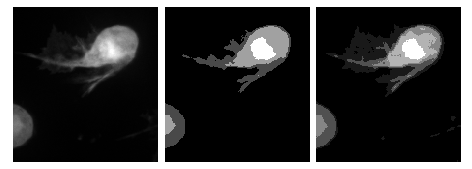
\includegraphics{img/fig_kmeans}
	\caption{Application of the K-Means algorithm to a test image. \textbf{Top left}: Input image. \textbf{Top right}: Ground truth labels of the input image. \textbf{Bottom left}: K-means results with $k=4$,  using arbitrary colors for the labels. \textbf{Bottom right}: Results with $k=6$. It is noteworthy that while the results for $k=4$ are reasonable, the nearly transparent lamellopodium pixels are labelled as background values, while the cell proper is segmented into two parts.}
	\label{fig:kmeans}
\end {figure}

\noindent Obviously, this algorithm can also be used to segment images into $k$ different classes, but since K-Means assigns classes to data by using the distance from the mean, the algorithm output favors segmentations in which the classes have roughly the same size, which isn't necessarily the correct way to classify pixels in arbitrary image data.

	\section{Canny Edge Detection}
The \textit{Canny Edge Detector} \cite{canny} is one of the most famous edge-detection algorithms and actually is a composite algorithm that returns a binary segmentation of an image into edges and non-edges.\\

\noindent First, a Gaussian convolution filter is applied to try and subdue noise in the image. A \textit{convolution} is a matrix operation often used in image processing: A matrix $A$, describing the pixel values of an image, is convolved pixel-wise with a convolution matrix $B$ with dimensions $n \times n$ - that is, for each pixel $p$ of $A$, the pixel's $n \times n$-neighborhood pixel values are summed up while being weighted according to corresponding value in $B$. The resulting sum is then assigned to the output matrix in place of the previous value of the center pixel, which intuitively assumes the distance-weighted average value of its neighborhood. In the case of pixels that lie on the edge of the matrix to be convoluted, out-of-bounds considerations have to be made: A constant value such as zero can be assumed for the pixels in the neighborhood that would lie ``outside'' of the image, the existing image values can be mirrored or clamped to provide a torus-like out-of-bounds handling, or the convolution can be done only on those pixels whose neighborhood fully lies inside of the image, resulting in smaller output images.

The aforementioned ``Gaussian filter'' or ``kernel'' is a matrix whose values are defined so that performing a convolution using that matrix approximates the behavior of the two-dimensional Gaussian function with uniform variances for its $x$- and $y$-dimensions:

\[ f(x, y) = \exp \left(- \left( \frac{\left(x - p_x \right)^2}{2\sigma^2} + \frac{ \left(y - p_y \right)^2}{2\sigma^2} \right) \right), \]

\noindent where $p$ is the center pixel of the current neighborhood. Subsequently, $p_x$ and $p_y$ are the coordinates of this pixel within the matrix and $\sigma$, the standard variance, acts as the smoothing constant. The higher this constant is, the stronger the blur effect becomes.

In Gaussian filters, the $\sigma$ constant is expressed through the dimensions of the matrix - the larger the filter matrix, the stronger the blur effect. An example for a $3 \times 3$ Gaussian filter is the following matrix:

\[ \frac{1}{16} \left [ \begin{tabular}{ccc}
				1& 2& 1\\
				2& 4& 2\\
				1& 2& 1 
			   \end{tabular} \right ]\]

\noindent The coefficient $\frac{1}{16}$ is equal to the sum of the matrix values and ensures that the convolution does not change the average image value. \cite[p. 41]{machine_vision}\\

\noindent As the second step, an gradient-based edge detector filter is applied to the smoothed image. The most famous of these is the \textit{Sobel filter} \cite{sobel}, which approximates the local partial derivatives $\frac{\partial I}{\partial x}$ and $\frac{\partial I}{\partial y}$ of each pixel of the image function $I(x, y)$, using the $3 \times 3$ neighborhood of that pixel. It is given by the following matrices\cite[pp. 113 -- 114]{machine_vision}:

\[ \text{Sobel}_x = \left [ \begin{tabular}{ccc}
				-1& 0& 1\\
				-2& 0& 2\\
				-1& 0& 1 
			   \end{tabular} \right ] \text{ and } 
\text{Sobel}_y = \left [ \begin{tabular}{ccc}
				1& 2& 1\\
				0& 0& 0\\
				-1& -2& 1 
			   \end{tabular} \right ] 
\]

\noindent The result of these convolutions are two images, $G_x$ and $G_y$, which represent the partial local derivatives of each pixel. The gradient image of the original input image $I$ is then defined as

\[G = |\nabla I| = \sqrt{{G_x}^2 + {G_y}^2}.\]

\noindent Additionally, the gradient direction of each pixel can be calculated from the derivative images by measuring the angle between the x-axis and the gradient pixel coordinates by employing the atan2 function:

\[G_\phi = \text{atan2}(G_y, G_x) \]

\noindent Using $G_\phi$, edge thinning via non-maximum suppression is applied to the gradient image as the third step in the algorithm: For each pixel, the gradient direction acts as a criterion to decide which two neighboring pixels, that are each on opposite sides (positive and negative direction of the gradient), should be compared to the current pixel. If the value of the current pixel is not larger than the two neighbors' values, the pixel's value is not a local maximum and is set to zero. The gradient direction angles can either be rounded so that each angle represents one of the north-south, west-east directions and so forth, or linear interpolation can be used.

In the final step, a hysteresis threshold is applied. This process consists of defining two thresholds, $\theta_{high}$ and $\theta_{low}$. The definition for the thresholding function as given in \ref{sec:thresholding} is slightly altered:

\[ T(I(x, y), \theta_{high}, \theta_{low}) =  \begin{cases}
							2 \text{ if } I(x, y) \, \geq \, \theta_{high} \\
							1 \text{ if } I(x, y) \, \geq \, \theta_{low} \text{ and } < \theta_{high} \\
			          				0 \text{ otherwise}
			   			        \end{cases}
\]

\noindent Pixels that have a value of $2$ are called strong pixels because they had values larger than the high threshold, whereas pixels with a value of $1$ are called weak pixels. Finally, the algorithm checks for each pixel if an 8-connected path between that pixel and a strong pixel exists - if not, then the pixel is dropped. This can be done with the help of connected component-finding algorithms by dropping each ``$1$''-component which is not connected to at least one ``2''-value.\\

\noindent The thresholds $\theta_{high}$ and $\theta_{low}$ have to be set by the user, although there exists the possibility to set these by using the Otsu threshold described in \ref{sec:thresholding} . Using this combination approach, $\theta_{high}$ is set to the Otsu threshold value for $I(x, y)$, and $\theta_{low}$ is set to $0.5 * \theta_{high}$.\cite{otsu_combine}


	\section{Gaussian Mixture Models}
Gaussian Mixtures Models (GMMs) are a subclass of mixture models, that is, probabilistic models which are combined with other models of the same distribution type to form a more complex model that is able to model the distribution of a data set more accurately than a simple model could. In the case of GMMs, the base distributions are often $n$-multivariate Gaussian distributions:

\[ pdf(x) = \mathcal{N}_n (x\,|\,\mu,\, \Sigma) \]

\noindent Here, $pdf(x)$ denotes the probability, or density, of an $n$-dimensional piece of data $x$, while $\mu$ and $\Sigma$ are the $n$-dimensional mean vector and the $n \times n$ covariance matrix of the distribution. Since the shape such a distribution can take is limited, a single Gaussian cannot accurately model a multimodal distribution (see Figure \ref{fig:normal_vs_gmm}). Instead, a weighted combination of multiple Gaussians can be used instead: \cite[pp. 430]{bishop_pattern}

\[ pdf_m (x) = \sum \limits_{k=1}^{K} \pi_k \, \mathcal{N}_n (x\,|\, \mu_k, \Sigma_k) \]

\noindent A mixture model consists of $K$ models that each have different parameters $\mu$ and $\Sigma$ and are weighted by weights $\pi_k \in \mathbb{R}$, $1 > \pi_k > 0$, with $\sum_{i=1}^{k} \pi_i = 1$.

\begin {figure}[!ht]
	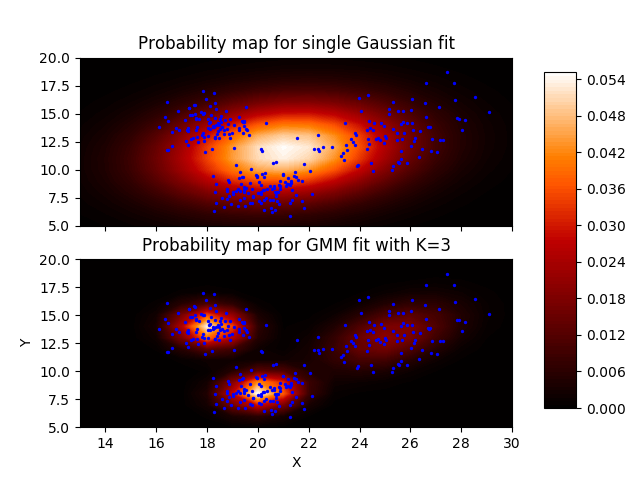
\includegraphics{img/fig_normal_vs_gmm}
	\caption{Comparison of a single Gaussian fit (upper) with a GMM fit, using $K=3$, on a two-dimensional dataset randomly sampled from three Gaussian distributions. The single Gaussian fails to capture the structure of the data, while the GMM succeeds.}
	\label{fig:normal_vs_gmm}
\end {figure}

\noindent The parameters of such a mixture model can be calculated by applying the Expectation-Maximization (EM) algorithm, which can additionally be combined with a K-Means initialization to avoid shallow local minima.\cite{em_algorithm} GMMs can also be used for segmenting images: Grayscale images are simply three-dimensional data in which each pixel coordinate corresponds to an intensity value. If the number of components to be found in the image is known beforehand, as it is in the case of cell segmentation, the intensity values can be segmented according to the fitted GMM (see Figure \ref{fig:gmm_vs_gt}). To do this, for each pixel in the image the posterior probabilities for that pixel in respect to each of the Gaussians is calculated and the Gaussian with the highest probability is chosen as the ``source'' of the pixel:

\[ label_x = \argmax \limits_{k} \, p(\mu_k, \Sigma_k\, | \, x) \]

\begin {figure}[!ht]
	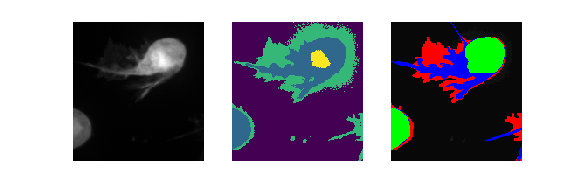
\includegraphics{img/fig_gmm_vs_gt}
	\caption{From left to right: Input image, pseudo-color labels assigned by a $K=4$ GMM fit to the input image and the ground truth labels for the input image.}
	\label{fig:gmm_vs_gt}
\end {figure}


	\section{Graph Cuts}



	\section{Multi-layer Perceptrons}
\textit{Multi-layer Perceptrons} (MLPs) or \textit{Feedforward Artificial Neuronal Networks} (ANNs) are mathematical functions that try to emulate the way neurons in the brain process information, typically to classify data or perform regression on it. ANNs have recently achieved impressing results on various tasks, such as image classification, sound analysis and regression, typically achieved by very deep networks that used lots of artificial neurons and were fed large datasets exceeding one million samples. In this section, the concepts behind optimization of functions via Gradient Descent, neuronal networks and training of those networks using the Backpropagation algorithm are explained. 



\subsection {Gradient Descent}
\label{subsec:grad_desc}

\textit{Gradient Descent} or the ``method of steepest descent'' is a standard, analytic first-order technique first introduced by that can be used to minimize or maximize at least once-differentiable functions, that is, to calculate a vector of parameters $\Theta$ for a function $f$ so that

\[ \Theta = \argmax \limits_{i} f(i) \]

\noindent To find values for $\Theta$, the approach takes advantage of the fact that the negative gradient vector $\nabla_f = [ \frac{\partial f}{\partial \Theta_0}, \dots, \frac{\partial f}{\partial \Theta_n} ]$, the vector of all first partial derivatives of $f$, points into the direction of the fastest change, or put graphically, the ``steepest slope''. By taking steps into the direction of this gradient, the function value is minimized step by step, while maximization works the same, only that the function is negated and then minimized, which results in parameters that maximize the original function. The parameter $\eta$ depicts the step size and is typically a value in the range $(0.0, 1.0]$. \cite[pp. 40--42]{optimization_book}

The algorithm starts with a guess for the parameters in $\Theta$ and then iteratively evaluates the gradient and updates the parameters accordingly until convergence within arbitrary precision is reached (see algorithm \ref{alg:grad_desc}).

\begin {algorithm}
	\begin {algorithmic}[1]
		\State $\Theta_0$ = random
		\While {$|f(\Theta_i) - f(\Theta_{i - 1})| > \epsilon$}
			\State $\Theta_i = \Theta_{i-1} - \eta \nabla_f$ 
		\EndWhile
	\end{algorithmic}
	\caption{Gradient Descent scheme for optimizing differentiable functions.}
	\label{alg:grad_desc}
\end{algorithm}

\noindent For convex functions, Gradient Descent always finds the global minimum. For non-convex functions however, the algorithm may get stuck in a local minimum or at saddle points, called ``false minima' (see figure \ref{fig:grad_desc}). Therefore, running the algorithm multiple times with random values or even informed guesses given knowledge about the form of the function to be optimized is advised. The step size $\eta$ has to be chosen depending on the shape of the function to minimize; if $\eta$ is too large, the algorithm will overshoot the minimum and never converges, even if the minimum exists, and if $\eta$ is too small, convergence will take a long time. Also, for some functions, the algorithm starts moving in a zig-zag pattern near the optimum, further increasing the number of steps the algorithm takes until covergence. To address these problems, a number of optimizations were proposed, some of which are discussed in section \ref{chapter_optimization}.


\begin {figure}[!ht]
	\begin{center}
		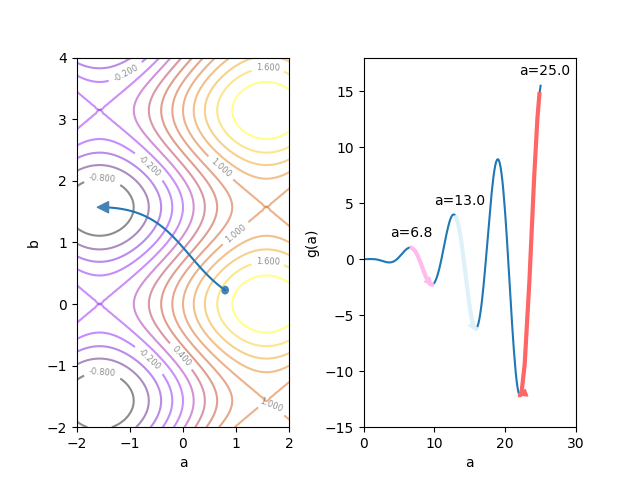
\includegraphics[scale=0.9]{img/fig_grad_desc}
	\end{center}
	\caption{\textbf{Left:} A contour plot of Gradient Descent minimization of $f(a, b) = \sin(a) + \cos^2(b)$. The blue line shows the search path of the algorithm along the negative gradient while estimating the optimal $\Theta$. \textbf{Right}: Effect of the initial guess for $\Theta$ on the optimization. The function $f(a) = \frac{1}{40}a^2 * \frac{1}{2} \cos(a)$ has multiple local minima in the interval [0, 25]. Only the third guess $a=25$ leads to finding the global minimum, while the other two optimization runs get trapped in local minima.}
	\label{fig:grad_desc}
\end {figure}


	\subsection{The Perceptron Algorithm}
\label{subsec:perceptron_algo}

A single-layer ANN is a network consisting of just one neuron, and is also called ``perceptron''. The idea for the perceptron was first proposed by Rosenblatt \cite{rosenblatt_report, rosenblatt_book}, who used it to perform binary classifications, using what is now called the ``perceptron algorithm''. Given a linearly separable set of $m$ data points of dimension $n$, one can construct a $(n+1) \times m$ input matrix $x$. The last entry in every column is set to $1$ to simplify the notation later on.

The \textit{perceptron classifier}, the function that decides which class a given sample belongs to, then takes the form of a linear function

\[ d(x) = h(w^{T}x), \label{eq:perc_class} \]

\noindent where $w$ is a vector of dimension $n+1$ and contains the $n$ \textit{weights} and the \textit{bias} value. The function $h$ is the \textit{activation function}, which is defined as 

\[ h(a) =  \begin{cases}
		+1 \text{ if } a \geq 0 \\
	   	 -1 \text{ otherwise}
	    \end{cases}\]

\noindent and maps its input to one of two possible classes.\\

\noindent The task of \textit{training} is defined as finding values for $w_0, \dots, w_{n+1}$ so that each data point is classified correctly by the resulting line, plane or (hyper-)plane. To this account, there needs to be a $m$-dimensional vector $t$ containing the \textit{labels} of each data point to verify the correctness of $w$. These labels are integers that indicate which class each data point belongs to. In the case of the perceptron algorithm, the labels are either $1$ for the first class $C_1$ or $-1$ for the second class, $C_2$. If all data points are classified correctly by some $w$, then it holds that

\[ w^T x_n \, t_n > 0 \,\,\forall\, x_n \in x \label{eq:perceptron_label} \]

\noindent Using this definition of correctness, a correctness measure can be formulated, which is known as the ``perceptron criterion''. Functions of this kind are also called \textit{error functions} or \textit{loss functions}. This particular loss function is given by

\[ E_p(w) = - \sum \limits_{n \in \mathcal{M}} w^T x_n\, t_n, \label{eq:perc_error}\]

\noindent where $\mathcal{M}$ is the set of all data points that were misclassfied, meaning that evaluating equation \ref{eq:perceptron_label} for that data yields a value $< 0$. \cite[pp. 192--194]{bishop_pattern}\\

\noindent The correct perceptron weights can then be determined by some arbitrary learning algorithm, although here, the Gradient Descent scheme (see algorithm \ref{alg:grad_desc}) is applied to the error function \ref{eq:perc_error}. When optimizing functions that not only depend on the parameters $\Theta$ but also on some dataset, one can consider one of the subtypes of Gradient Descent; either, evaluating the average gradient using all available data samples (\textit{Batch Gradient Descent}) or using single data points only - as an approximation of the entire dataset - to perform the updates. This is called \textit{Stochastic Gradient Descent} (SGD) and is preferable if working with datasets that are too large to fit into memory. Alternatively, one can use the average gradient of a subset of data points - this method is often referred to as \textit{Mini-Batch} Gradient Descent.

Either way, the gradient of $E_p$ has to be calculated. The perceptron criterion only depends on the weights $w$, so the gradient vector has the shape

\[ \nabla_E = \left[ \frac{\partial E_p}{\partial w_0}, \frac{\partial E_p}{\partial w_1}, \dots, \frac{\partial E_p}{\partial w_{n+1}} \right ] \,. \]

\noindent Taking the partial derivatives in respect to $w$ leads to

\begin{align}
 	\nabla_E &= \frac{\partial E_p}{\partial w} = \frac{\partial}{\partial w} \left (- \sum \limits_{n \in \mathcal{M}} w^T x_n t_n \right ) \\
 	&= -\sum \limits_{n \in \mathcal{M}} x_n t_n
\end{align}

\noindent If SGD is used, this is reduced to simply

\[ \nabla_E = -x_n t_n\]

\noindent for some previously misclassified point $x_n \in \mathcal{M}$ in the dataset. Hence, the update rule for the perceptron becomes

\[w_i = w_{i - 1} + x_n t_n * \eta\]

\noindent Using this update rule leads to the training algorithm shown in \ref{alg:perceptron_algorithm}, which is applied to an example dataset in figure \ref{fig:perceptron}.

\begin {figure}[!ht]
	\begin{center}
		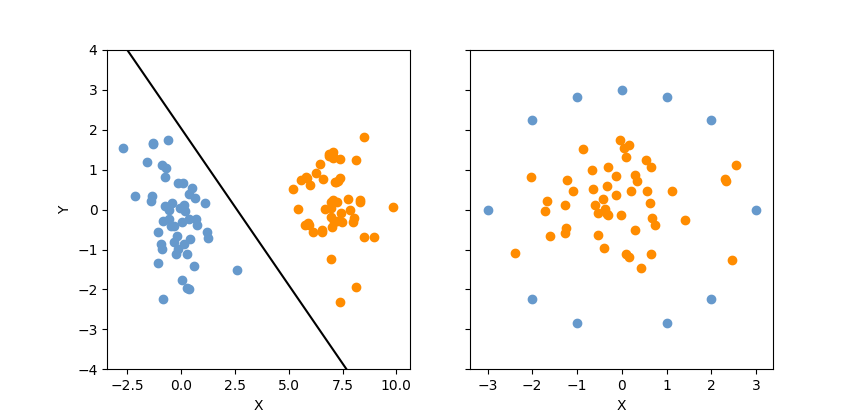
\includegraphics[scale=0.6]{img/fig_perceptron}
	\end{center}
	\caption{\textbf{Left}: Separating two datasets with the perceptron algorithm in $\mathbb{R}^2$. The correct classification boundary takes the form of a line, i.e. $0 = w^{T}x = w_0 x + w_1 y + w_2$. The line pictured is given by $w = (-2.285, -2.908, 5.938)$, the weights after 19 iterations. \textbf{Right}: A not-linearly separable data set, on which the algorithm would never converge, because it is based on finding linear classifiers and thus cannot separate the data correctly.}
	\label{fig:perceptron}
\end {figure}

\begin {algorithm}
	\begin {algorithmic}[1]
		\State $w$ = random
		\While {true}
			\For{$x_i$ in $x$}
				\If{$w^T x_i t_i \leq 0$}
					\State $w$ += $x_i t_i * \eta$
				\EndIf

				\If{$w^T x_i t_i > 0$ for all $x_i$ in $x$}
					\State stop
				\EndIf
			\EndFor
		\EndWhile
	\end{algorithmic}
	\caption{Stochastic Gradient Descent applied to the task of finding the perceptron weights $w$. $x$ is assumed to be linearly separable.}
	\label{alg:perceptron_algorithm}
\end{algorithm}



		\subsection{Multiple Neurons and Backpropagation}
While the perceptron algorithm works fine for linear problems, those are only a small subset of real-world problems (see figure \ref{fig:perceptron}). The solution to this problem is to add more neurons to the model, which form a network that consists of layers that pass the outputs of neurons in the previous layers through non-linear activation functions and then use the results as inputs. These layers are referred to as the ``input layer'', the initial layer, the ``output layer'', the last layer, and ``hidden layers'', which are all the layers inbetween.

The resulting networks are called \textit{Multi-Layer Perceptrons} (MLPs), \textit{Feedforward Artificial Neural Networks}(ANNs), or, in the case of a multitude of layers, \textit{Deep Neural Networks}, and are much more powerful than simple perceptrons, as they can approximate haphazard continuous functions that operate on closed and bounded subsets of $\mathbb{R}^n$ given that the network possesses at least one hidden layer of neurons. This capability makes using MLPs for learning real-life problems feasible.\cite{universal_approx}\cite{universal_approx2}\\

\noindent Again, each neuron in the network computes a weighted sum of its $i$ inputs, just like in equation \ref{eq:perc_class}, although indexing has been added to identify neurons and weights in the entire network:

\[ a_j^{(l)} = \sum \limits_{i} w^{(l)}_{ji}\,\, y_i + b^{(l)}_{j} \]

\noindent $y_i$ are the input values to the current neuron. Note that these either are the direct inputs $x_i$ to the network, or outputs of other neurons, depending on where in the network the term is evaluated. $w$ is the matrix of weights, and $w^{(l)}_{ji}$ denotes the weight of the connection from the $i$th neuron in the previous layer $l - 1$ to the $j$th neuron in the  layer $l$. The term $b$ is the bias weight associated with the neuron $j$. The bias can be made part of the weight matrix by introducing an additional input dimension with a value of $1$, like it was done for the perceptron algorithm in section \ref{subsec:perceptron_algo}.

Afterwards, the sum $a^{(l)}_j$ is passed into an activation function $h(\cdot)$ to produce the activation of the $j$th neuron in the $l$th layer, $z_j^{(l)}$:

\[ z_j^{(l)} = h(a^{(l)}_j) \]

\noindent In vectorized notation, the activations of an entire layer could therefore be written as the recursive formula

\[ z^{(l)} = h(w^{(l)} z^{(l-1)}) \cite{nielsen_book} \]

\noindent where the activations of the input layer are simply the inputs themselves, thus ending the recursion. Expanding the term for the 2-layer network shown in figure \ref{fig:mlp} gives the following formula for a network output $out_k$:

\[ out_k = \sigma \left ( \sum \limits_{j=0}^{4} w^{(2)}_{kj}\,\, h \left ( \sum \limits_{i=0}^{3} w^{(1)}_{ji} x_i \right ) \right ) \label{eq:mlp_out} \]

\noindent Here, \textbf{$\sigma$} is an output function that is applied in the last layer of the network, and is dependent on the task the network is supposed to fulfill: For regression problems, fitting a function to a set of data and then predicting new values using that function, the identity function can be used, but for binary classification problems, instead of using a step function like in the original perceptron, one instead uses the continuous \textit{Sigmoid} function and interprets the output as

\[ \sigma_{sig}(x_i) = \begin{cases}
				x_i \in C_1 \text{ if } \frac{1}{1 + e^{-x_i}} \geq 0.5 \\
				x_i \in C_2 \text{ else }\\
			 \end{cases}
\]

\noindent Also, the choice of the activation function $h(w, x)$ is different from the perceptron: It is not chosen to be the Heaviside function, but instead, to be a non-linear, continuous and differentiable function. Computing an output is done by passing the input vector to the first layer, which computes its activations for all its neurons, which then pass on their activations to the neurons of the next layer as inputs until the output layer is reached.

If the classification is non-binary, using the \textit{Softmax} function (see section \ref{subsec:softmax}) to obtain probabilities for the likeliness of $x_i$ being part of any of the classes is a solution.\\

\afterpage{
	\begin {figure}[!ht]
		\begin{center}
			\def\svgwidth{0.8\columnwidth}
			\input{img/mlp.pdf_tex}
		\end{center}
		\caption[]{An MLP with one hidden layer, forming an acyclic directed graph, where connections are color-coded per layer by the receiving neuron. The layer count $L$ starts at the layer after the input layer\protect\footnotemark. Therefore $L = 2$, with three inputs $x_i$ and neuron counts $D^{(1)} = 4$ and $D^{(2)} = 2$. The variables $b^{(1)}$ and $b^{(2)}$ refer to the biases for the neurons in the layers $(1)$ or $(2)$, respectively. Each neuron has its own, changeable bias value, but for the sake of cleanness, the connections from the biases to each neuron of their corresponding layer are not shown.}
		\label{fig:mlp}
	\end {figure}

	\footnotetext{There is no consensus on which method of counting is the most appropriate. Sometimes, only the number of hidden layers or even all layers are counted \cite[pp. 229]{bishop_pattern}}
}

\noindent The goal of training an MLP is - as previously for the perceptron - finding specific weights so that all inputs are classified correctly, or at least, so that the network makes only few mistakes. Therefore, a loss layer is added to the end of the network, measuring the correctness of the output. Instead of the perceptron criterion \ref{eq:perc_error}, a more general loss function is employed which compares the difference between the output $\sigma(x)$ of the network for a sample $x$ and the preferred output for $x$, the \textit{label} or \textit{ground truth} of $x$. Typically, the loss function for regression problems is based on the \textit{Least Squares Error} (LSE), which is defined as

\[ LSE(w) = \frac{1}{2} \left ( out - t \right )^2, \]

\noindent where the single, linear output of the network for some input $x$ and a set of weights $w$ is compared to the ground truth $t$.\footnote{The error is only given as a function of $w$ because both the input $x$ and its correct label $t$ are fixed in the particular case presented here.} Binary classification problems instead use Sigmoid outputs together with the \textit{Cross-Entropy} loss function, which is defined as 

\[ CE(w) =  -t \, \ln out + (1 - t) \ln (1 - out). \]

\noindent For multi-class classifications, an adaption of the Cross-Entropy loss can be used, which is further described in section \ref{subsec:cross_ent}. \cite[pp. 232-236]{bishop_pattern}\\

\noindent Training a network with multiple layers is harder than training a single perceptron because the influence of each of the weights in any layer of the network on the error function has to be computed when using gradient-based optimization methods while the output of the network no longer is the result of a single function, but instead, a composition of a usually large number of functions (see equation \ref{eq:mlp_out}). Although it is possible to manually calculate the partial derivatives for the entire network, this becomes more and more cumbersome as the network grows in size.

Luckily, there exists an iterative algorithm called \textit{Backpropagation} \cite{backprop} that finds the gradient of the loss with respect to each weight so that an optimization method can be applied to change every weight. The algorithm makes use of the fact that each neuron can be viewed (almost) independently from the rest of the network. Remembering that the analytic way of obtaining the derivative of a composition of functions 

\[ f \circ g = f(g(x)) \]

\noindent with respect to some $x$ is to apply the chain rule

\[ \frac{\partial f}{\partial x} =\frac{\partial f}{\partial g} \frac{\partial g}{\partial x} \, , \]

\noindent one can see that this concept can also be applied to neurons in a network, because using the output value of a neuron in a previous layer as the input for a node is nothing else than function composition.\\

\noindent Backpropagation thus starts with a \textit{forward pass}, which means that an input vector $x$ is passed through the network and the corresponding sums $a_j$ and activations $z_j$ are calculated and stored. Comparing the final outputs to the ground truth in the loss layer, the network is then traversed in the opposite direction in what is called a \textit{backward pass}, aiming to obtain the influence of each weight in each layer on the final loss, that is, the gradient of the loss function with respect to the weights. After this first phase, the partial derivatives for each weight are known, and the weights are updated in a second phase, in which an optimization algorithm like Gradient Descent is used as described in section \ref{subsec:grad_desc}.\\

\noindent The central idea of the backward pass is that when traversing the network from the output layer to the input layer, the derivatives of the loss function with respect to weights of a layer depend on weights of the layers that precede them. This relationship is described by the formula

\begin {align}
	\frac{\partial E}{\partial w_{ji}} &= \frac{\partial E}{\partial a_j} \frac{\partial a_j}{\partial w_{ji}}
\end {align}

\noindent where $E$ is the loss function of the network. According to the chain rule, the influence of the weight $w_{ji}$ on the loss is equal to the influence of the weight on the sum of inputs $a_j$ times the influence of $a_j$ on the loss function. In literature, the term $\frac{\partial E}{\partial a_j}$ is often denoted as $\delta_j^{(l)}$, the ``error'' of the neuron $j$ in layer $l$. Using this notation and taking the partial derivative of the weighted sum $a_j$, the formula becomes

\[ \frac{\partial E}{\partial w_{ji}} = \delta_j^{(l)} z_i .\]

\noindent Since $z_i$, the activation from the input end of the connection that is modified by $w_{ji}$, is already known for all neurons due to the forward pass, the only thing that needs to be computed to figure out the loss gradient are the $\delta$-values. The computation of $\delta_j^{(l)}$ depends on the position of the neuron in the network:

\[ \delta_j^{(l)} =  \begin{cases}
				\frac{\partial E}{\partial a_j} \text{ if neuron } j^{(l)} \text{ is an output neuron} \\
			           h'(a_j) \sum \limits_{k} w_{kj} \, \delta_k^{(l+1)} \text{ otherwise}
			     \end{cases}
\]

\noindent In the case $j$ is an output neuron, the partial is calculated directly. Otherwise, $\delta_j$ depends on the $\delta$-values in the previous layers, necessitating the backward traversion (see figure \ref{fig:backprop}). The definition of $\delta$ for hidden neurons is also the reason why a differentiable function must be chosen as the activation $h(\cdot)$, as stated earlier.\\

\noindent The main advantage of the algorithm is that it scales linearly with the number of weights, i.e. the algorithm is $\in \mathcal{O}(w)$. Furthermore, the fact that all $\delta$-values of a layer have to be calculated to calculate all $\delta$ values and weight derivatives in the layer that precedes it naturally leads to vectorizing the algorithm layerwise in efficient implementations. \cite{nielsen_book}\cite{ng_lecture}\cite[pp. 241-245]{bishop_pattern}


\afterpage{
	\begin {figure}[!ht]
		\begin{center}
			\def\svgwidth{0.8\columnwidth}
			\input{img/backprop.pdf_tex}
		\end{center}
		\caption[]{Backpropagation algorithm, applied to a hidden layer $l$\protect\footnotemark. Steps during the forward pass are shown in blue, while steps during the backward pass are orange. The central neuron is the only neuron in the layer $l$, while there are two neurons each in the layers $l-1$ and $l+1$. These other layers could be other hidden layers, input layers, or output layers, as the computation is generalized by the definition of $\delta$. The forward pass calculates the weighted sum $a_1^{(l)}$ and the activation $h(a_1^{(l)})$. Once the backward pass reaches the neuron, it calculates $\delta_1^{(l)}$ and the partial derivatives of the weights of layer $l$, that is, the weights of the connections that flow into the central neuron in the forward pass, using the backpropagated value $\delta_k^{(l+1)}$. This is repeated throughout the entire network until the entire weight gradient is known and a single Gradient Descent step can be taken toward the loss function minimum.}
		\label{fig:backprop}
	\end {figure}

	\footnotetext{This example is based on a visualization in \cite{karparthy_lecture}.}
}

\noindent Depending on how deep the networks are, i.e. how many hidden layers there are and how many neurons there are in these hidden layers, neural networks can learn very complex classification boundaries. The role of the activation function is akin to the kernel principle of State Vector Machines (SVMs), since it maps inputs to higher-dimensional spaces in which they are linearly separable by a hyperplane (see figure \ref{fig:mlp_trick}).

\begin {figure}[!ht]
		\begin{center}
			%% Creator: Matplotlib, PGF backend
%%
%% To include the figure in your LaTeX document, write
%%   \input{<filename>.pgf}
%%
%% Make sure the required packages are loaded in your preamble
%%   \usepackage{pgf}
%%
%% Figures using additional raster images can only be included by \input if
%% they are in the same directory as the main LaTeX file. For loading figures
%% from other directories you can use the `import` package
%%   \usepackage{import}
%% and then include the figures with
%%   \import{<path to file>}{<filename>.pgf}
%%
%% Matplotlib used the following preamble
%%   \usepackage{fontspec}
%%   \setmainfont{DejaVu Serif}
%%   \setsansfont{DejaVu Sans}
%%   \setmonofont{DejaVu Sans Mono}
%%
\begingroup%
\makeatletter%
\begin{pgfpicture}%
\pgfpathrectangle{\pgfpointorigin}{\pgfqpoint{6.510000in}{1.550000in}}%
\pgfusepath{use as bounding box, clip}%
\begin{pgfscope}%
\pgfsetbuttcap%
\pgfsetmiterjoin%
\definecolor{currentfill}{rgb}{1.000000,1.000000,1.000000}%
\pgfsetfillcolor{currentfill}%
\pgfsetlinewidth{0.000000pt}%
\definecolor{currentstroke}{rgb}{1.000000,1.000000,1.000000}%
\pgfsetstrokecolor{currentstroke}%
\pgfsetdash{}{0pt}%
\pgfpathmoveto{\pgfqpoint{0.000000in}{0.000000in}}%
\pgfpathlineto{\pgfqpoint{6.510000in}{0.000000in}}%
\pgfpathlineto{\pgfqpoint{6.510000in}{1.550000in}}%
\pgfpathlineto{\pgfqpoint{0.000000in}{1.550000in}}%
\pgfpathclose%
\pgfusepath{fill}%
\end{pgfscope}%
\begin{pgfscope}%
\pgfsetbuttcap%
\pgfsetmiterjoin%
\definecolor{currentfill}{rgb}{1.000000,1.000000,1.000000}%
\pgfsetfillcolor{currentfill}%
\pgfsetlinewidth{0.000000pt}%
\definecolor{currentstroke}{rgb}{0.000000,0.000000,0.000000}%
\pgfsetstrokecolor{currentstroke}%
\pgfsetstrokeopacity{0.000000}%
\pgfsetdash{}{0pt}%
\pgfpathmoveto{\pgfqpoint{0.584722in}{0.387222in}}%
\pgfpathlineto{\pgfqpoint{1.556778in}{0.387222in}}%
\pgfpathlineto{\pgfqpoint{1.556778in}{1.365000in}}%
\pgfpathlineto{\pgfqpoint{0.584722in}{1.365000in}}%
\pgfpathclose%
\pgfusepath{fill}%
\end{pgfscope}%
\begin{pgfscope}%
\pgfpathrectangle{\pgfqpoint{0.584722in}{0.387222in}}{\pgfqpoint{0.972056in}{0.977778in}} %
\pgfusepath{clip}%
\pgfsetbuttcap%
\pgfsetroundjoin%
\definecolor{currentfill}{rgb}{0.960000,0.895056,0.816000}%
\pgfsetfillcolor{currentfill}%
\pgfsetlinewidth{1.003750pt}%
\definecolor{currentstroke}{rgb}{0.960000,0.895056,0.816000}%
\pgfsetstrokecolor{currentstroke}%
\pgfsetdash{}{0pt}%
\pgfpathmoveto{\pgfqpoint{1.165798in}{0.632376in}}%
\pgfpathcurveto{\pgfqpoint{1.171621in}{0.632376in}}{\pgfqpoint{1.177208in}{0.634690in}}{\pgfqpoint{1.181326in}{0.638808in}}%
\pgfpathcurveto{\pgfqpoint{1.185444in}{0.642926in}}{\pgfqpoint{1.187758in}{0.648512in}}{\pgfqpoint{1.187758in}{0.654336in}}%
\pgfpathcurveto{\pgfqpoint{1.187758in}{0.660160in}}{\pgfqpoint{1.185444in}{0.665746in}}{\pgfqpoint{1.181326in}{0.669864in}}%
\pgfpathcurveto{\pgfqpoint{1.177208in}{0.673982in}}{\pgfqpoint{1.171621in}{0.676296in}}{\pgfqpoint{1.165798in}{0.676296in}}%
\pgfpathcurveto{\pgfqpoint{1.159974in}{0.676296in}}{\pgfqpoint{1.154387in}{0.673982in}}{\pgfqpoint{1.150269in}{0.669864in}}%
\pgfpathcurveto{\pgfqpoint{1.146151in}{0.665746in}}{\pgfqpoint{1.143837in}{0.660160in}}{\pgfqpoint{1.143837in}{0.654336in}}%
\pgfpathcurveto{\pgfqpoint{1.143837in}{0.648512in}}{\pgfqpoint{1.146151in}{0.642926in}}{\pgfqpoint{1.150269in}{0.638808in}}%
\pgfpathcurveto{\pgfqpoint{1.154387in}{0.634690in}}{\pgfqpoint{1.159974in}{0.632376in}}{\pgfqpoint{1.165798in}{0.632376in}}%
\pgfpathclose%
\pgfusepath{stroke,fill}%
\end{pgfscope}%
\begin{pgfscope}%
\pgfpathrectangle{\pgfqpoint{0.584722in}{0.387222in}}{\pgfqpoint{0.972056in}{0.977778in}} %
\pgfusepath{clip}%
\pgfsetbuttcap%
\pgfsetroundjoin%
\definecolor{currentfill}{rgb}{0.960000,0.859517,0.737199}%
\pgfsetfillcolor{currentfill}%
\pgfsetlinewidth{1.003750pt}%
\definecolor{currentstroke}{rgb}{0.960000,0.859517,0.737199}%
\pgfsetstrokecolor{currentstroke}%
\pgfsetdash{}{0pt}%
\pgfpathmoveto{\pgfqpoint{1.058174in}{0.823801in}}%
\pgfpathcurveto{\pgfqpoint{1.064829in}{0.823801in}}{\pgfqpoint{1.071212in}{0.826446in}}{\pgfqpoint{1.075918in}{0.831151in}}%
\pgfpathcurveto{\pgfqpoint{1.080624in}{0.835857in}}{\pgfqpoint{1.083268in}{0.842241in}}{\pgfqpoint{1.083268in}{0.848896in}}%
\pgfpathcurveto{\pgfqpoint{1.083268in}{0.855551in}}{\pgfqpoint{1.080624in}{0.861935in}}{\pgfqpoint{1.075918in}{0.866641in}}%
\pgfpathcurveto{\pgfqpoint{1.071212in}{0.871346in}}{\pgfqpoint{1.064829in}{0.873991in}}{\pgfqpoint{1.058174in}{0.873991in}}%
\pgfpathcurveto{\pgfqpoint{1.051519in}{0.873991in}}{\pgfqpoint{1.045135in}{0.871346in}}{\pgfqpoint{1.040429in}{0.866641in}}%
\pgfpathcurveto{\pgfqpoint{1.035723in}{0.861935in}}{\pgfqpoint{1.033079in}{0.855551in}}{\pgfqpoint{1.033079in}{0.848896in}}%
\pgfpathcurveto{\pgfqpoint{1.033079in}{0.842241in}}{\pgfqpoint{1.035723in}{0.835857in}}{\pgfqpoint{1.040429in}{0.831151in}}%
\pgfpathcurveto{\pgfqpoint{1.045135in}{0.826446in}}{\pgfqpoint{1.051519in}{0.823801in}}{\pgfqpoint{1.058174in}{0.823801in}}%
\pgfpathclose%
\pgfusepath{stroke,fill}%
\end{pgfscope}%
\begin{pgfscope}%
\pgfpathrectangle{\pgfqpoint{0.584722in}{0.387222in}}{\pgfqpoint{0.972056in}{0.977778in}} %
\pgfusepath{clip}%
\pgfsetbuttcap%
\pgfsetroundjoin%
\definecolor{currentfill}{rgb}{0.960000,0.831877,0.675914}%
\pgfsetfillcolor{currentfill}%
\pgfsetlinewidth{1.003750pt}%
\definecolor{currentstroke}{rgb}{0.960000,0.831877,0.675914}%
\pgfsetstrokecolor{currentstroke}%
\pgfsetdash{}{0pt}%
\pgfpathmoveto{\pgfqpoint{1.032954in}{0.803443in}}%
\pgfpathcurveto{\pgfqpoint{1.040189in}{0.803443in}}{\pgfqpoint{1.047130in}{0.806317in}}{\pgfqpoint{1.052246in}{0.811434in}}%
\pgfpathcurveto{\pgfqpoint{1.057363in}{0.816551in}}{\pgfqpoint{1.060238in}{0.823491in}}{\pgfqpoint{1.060238in}{0.830727in}}%
\pgfpathcurveto{\pgfqpoint{1.060238in}{0.837963in}}{\pgfqpoint{1.057363in}{0.844903in}}{\pgfqpoint{1.052246in}{0.850020in}}%
\pgfpathcurveto{\pgfqpoint{1.047130in}{0.855137in}}{\pgfqpoint{1.040189in}{0.858011in}}{\pgfqpoint{1.032954in}{0.858011in}}%
\pgfpathcurveto{\pgfqpoint{1.025718in}{0.858011in}}{\pgfqpoint{1.018777in}{0.855137in}}{\pgfqpoint{1.013661in}{0.850020in}}%
\pgfpathcurveto{\pgfqpoint{1.008544in}{0.844903in}}{\pgfqpoint{1.005669in}{0.837963in}}{\pgfqpoint{1.005669in}{0.830727in}}%
\pgfpathcurveto{\pgfqpoint{1.005669in}{0.823491in}}{\pgfqpoint{1.008544in}{0.816551in}}{\pgfqpoint{1.013661in}{0.811434in}}%
\pgfpathcurveto{\pgfqpoint{1.018777in}{0.806317in}}{\pgfqpoint{1.025718in}{0.803443in}}{\pgfqpoint{1.032954in}{0.803443in}}%
\pgfpathclose%
\pgfusepath{stroke,fill}%
\end{pgfscope}%
\begin{pgfscope}%
\pgfpathrectangle{\pgfqpoint{0.584722in}{0.387222in}}{\pgfqpoint{0.972056in}{0.977778in}} %
\pgfusepath{clip}%
\pgfsetbuttcap%
\pgfsetroundjoin%
\definecolor{currentfill}{rgb}{0.960000,0.895056,0.816000}%
\pgfsetfillcolor{currentfill}%
\pgfsetlinewidth{1.003750pt}%
\definecolor{currentstroke}{rgb}{0.960000,0.895056,0.816000}%
\pgfsetstrokecolor{currentstroke}%
\pgfsetdash{}{0pt}%
\pgfpathmoveto{\pgfqpoint{1.172847in}{0.553974in}}%
\pgfpathcurveto{\pgfqpoint{1.178671in}{0.553974in}}{\pgfqpoint{1.184257in}{0.556288in}}{\pgfqpoint{1.188375in}{0.560406in}}%
\pgfpathcurveto{\pgfqpoint{1.192493in}{0.564524in}}{\pgfqpoint{1.194807in}{0.570111in}}{\pgfqpoint{1.194807in}{0.575934in}}%
\pgfpathcurveto{\pgfqpoint{1.194807in}{0.581758in}}{\pgfqpoint{1.192493in}{0.587345in}}{\pgfqpoint{1.188375in}{0.591463in}}%
\pgfpathcurveto{\pgfqpoint{1.184257in}{0.595581in}}{\pgfqpoint{1.178671in}{0.597895in}}{\pgfqpoint{1.172847in}{0.597895in}}%
\pgfpathcurveto{\pgfqpoint{1.167023in}{0.597895in}}{\pgfqpoint{1.161437in}{0.595581in}}{\pgfqpoint{1.157319in}{0.591463in}}%
\pgfpathcurveto{\pgfqpoint{1.153201in}{0.587345in}}{\pgfqpoint{1.150887in}{0.581758in}}{\pgfqpoint{1.150887in}{0.575934in}}%
\pgfpathcurveto{\pgfqpoint{1.150887in}{0.570111in}}{\pgfqpoint{1.153201in}{0.564524in}}{\pgfqpoint{1.157319in}{0.560406in}}%
\pgfpathcurveto{\pgfqpoint{1.161437in}{0.556288in}}{\pgfqpoint{1.167023in}{0.553974in}}{\pgfqpoint{1.172847in}{0.553974in}}%
\pgfpathclose%
\pgfusepath{stroke,fill}%
\end{pgfscope}%
\begin{pgfscope}%
\pgfpathrectangle{\pgfqpoint{0.584722in}{0.387222in}}{\pgfqpoint{0.972056in}{0.977778in}} %
\pgfusepath{clip}%
\pgfsetbuttcap%
\pgfsetroundjoin%
\definecolor{currentfill}{rgb}{0.960000,0.895056,0.816000}%
\pgfsetfillcolor{currentfill}%
\pgfsetlinewidth{1.003750pt}%
\definecolor{currentstroke}{rgb}{0.960000,0.895056,0.816000}%
\pgfsetstrokecolor{currentstroke}%
\pgfsetdash{}{0pt}%
\pgfpathmoveto{\pgfqpoint{1.169637in}{0.664488in}}%
\pgfpathcurveto{\pgfqpoint{1.175461in}{0.664488in}}{\pgfqpoint{1.181047in}{0.666802in}}{\pgfqpoint{1.185165in}{0.670920in}}%
\pgfpathcurveto{\pgfqpoint{1.189284in}{0.675038in}}{\pgfqpoint{1.191598in}{0.680625in}}{\pgfqpoint{1.191598in}{0.686448in}}%
\pgfpathcurveto{\pgfqpoint{1.191598in}{0.692272in}}{\pgfqpoint{1.189284in}{0.697859in}}{\pgfqpoint{1.185165in}{0.701977in}}%
\pgfpathcurveto{\pgfqpoint{1.181047in}{0.706095in}}{\pgfqpoint{1.175461in}{0.708409in}}{\pgfqpoint{1.169637in}{0.708409in}}%
\pgfpathcurveto{\pgfqpoint{1.163813in}{0.708409in}}{\pgfqpoint{1.158227in}{0.706095in}}{\pgfqpoint{1.154109in}{0.701977in}}%
\pgfpathcurveto{\pgfqpoint{1.149991in}{0.697859in}}{\pgfqpoint{1.147677in}{0.692272in}}{\pgfqpoint{1.147677in}{0.686448in}}%
\pgfpathcurveto{\pgfqpoint{1.147677in}{0.680625in}}{\pgfqpoint{1.149991in}{0.675038in}}{\pgfqpoint{1.154109in}{0.670920in}}%
\pgfpathcurveto{\pgfqpoint{1.158227in}{0.666802in}}{\pgfqpoint{1.163813in}{0.664488in}}{\pgfqpoint{1.169637in}{0.664488in}}%
\pgfpathclose%
\pgfusepath{stroke,fill}%
\end{pgfscope}%
\begin{pgfscope}%
\pgfpathrectangle{\pgfqpoint{0.584722in}{0.387222in}}{\pgfqpoint{0.972056in}{0.977778in}} %
\pgfusepath{clip}%
\pgfsetbuttcap%
\pgfsetroundjoin%
\definecolor{currentfill}{rgb}{0.960000,0.818746,0.646798}%
\pgfsetfillcolor{currentfill}%
\pgfsetlinewidth{1.003750pt}%
\definecolor{currentstroke}{rgb}{0.960000,0.818746,0.646798}%
\pgfsetstrokecolor{currentstroke}%
\pgfsetdash{}{0pt}%
\pgfpathmoveto{\pgfqpoint{0.995274in}{0.965390in}}%
\pgfpathcurveto{\pgfqpoint{1.002770in}{0.965390in}}{\pgfqpoint{1.009960in}{0.968368in}}{\pgfqpoint{1.015261in}{0.973669in}}%
\pgfpathcurveto{\pgfqpoint{1.020561in}{0.978969in}}{\pgfqpoint{1.023539in}{0.986159in}}{\pgfqpoint{1.023539in}{0.993655in}}%
\pgfpathcurveto{\pgfqpoint{1.023539in}{1.001151in}}{\pgfqpoint{1.020561in}{1.008341in}}{\pgfqpoint{1.015261in}{1.013642in}}%
\pgfpathcurveto{\pgfqpoint{1.009960in}{1.018942in}}{\pgfqpoint{1.002770in}{1.021921in}}{\pgfqpoint{0.995274in}{1.021921in}}%
\pgfpathcurveto{\pgfqpoint{0.987778in}{1.021921in}}{\pgfqpoint{0.980588in}{1.018942in}}{\pgfqpoint{0.975287in}{1.013642in}}%
\pgfpathcurveto{\pgfqpoint{0.969987in}{1.008341in}}{\pgfqpoint{0.967009in}{1.001151in}}{\pgfqpoint{0.967009in}{0.993655in}}%
\pgfpathcurveto{\pgfqpoint{0.967009in}{0.986159in}}{\pgfqpoint{0.969987in}{0.978969in}}{\pgfqpoint{0.975287in}{0.973669in}}%
\pgfpathcurveto{\pgfqpoint{0.980588in}{0.968368in}}{\pgfqpoint{0.987778in}{0.965390in}}{\pgfqpoint{0.995274in}{0.965390in}}%
\pgfpathclose%
\pgfusepath{stroke,fill}%
\end{pgfscope}%
\begin{pgfscope}%
\pgfpathrectangle{\pgfqpoint{0.584722in}{0.387222in}}{\pgfqpoint{0.972056in}{0.977778in}} %
\pgfusepath{clip}%
\pgfsetbuttcap%
\pgfsetroundjoin%
\definecolor{currentfill}{rgb}{0.960000,0.682856,0.345490}%
\pgfsetfillcolor{currentfill}%
\pgfsetlinewidth{1.003750pt}%
\definecolor{currentstroke}{rgb}{0.960000,0.682856,0.345490}%
\pgfsetstrokecolor{currentstroke}%
\pgfsetdash{}{0pt}%
\pgfpathmoveto{\pgfqpoint{0.916056in}{0.568475in}}%
\pgfpathcurveto{\pgfqpoint{0.925847in}{0.568475in}}{\pgfqpoint{0.935238in}{0.572364in}}{\pgfqpoint{0.942160in}{0.579287in}}%
\pgfpathcurveto{\pgfqpoint{0.949083in}{0.586210in}}{\pgfqpoint{0.952973in}{0.595601in}}{\pgfqpoint{0.952973in}{0.605391in}}%
\pgfpathcurveto{\pgfqpoint{0.952973in}{0.615182in}}{\pgfqpoint{0.949083in}{0.624573in}}{\pgfqpoint{0.942160in}{0.631496in}}%
\pgfpathcurveto{\pgfqpoint{0.935238in}{0.638418in}}{\pgfqpoint{0.925847in}{0.642308in}}{\pgfqpoint{0.916056in}{0.642308in}}%
\pgfpathcurveto{\pgfqpoint{0.906266in}{0.642308in}}{\pgfqpoint{0.896875in}{0.638418in}}{\pgfqpoint{0.889952in}{0.631496in}}%
\pgfpathcurveto{\pgfqpoint{0.883029in}{0.624573in}}{\pgfqpoint{0.879140in}{0.615182in}}{\pgfqpoint{0.879140in}{0.605391in}}%
\pgfpathcurveto{\pgfqpoint{0.879140in}{0.595601in}}{\pgfqpoint{0.883029in}{0.586210in}}{\pgfqpoint{0.889952in}{0.579287in}}%
\pgfpathcurveto{\pgfqpoint{0.896875in}{0.572364in}}{\pgfqpoint{0.906266in}{0.568475in}}{\pgfqpoint{0.916056in}{0.568475in}}%
\pgfpathclose%
\pgfusepath{stroke,fill}%
\end{pgfscope}%
\begin{pgfscope}%
\pgfpathrectangle{\pgfqpoint{0.584722in}{0.387222in}}{\pgfqpoint{0.972056in}{0.977778in}} %
\pgfusepath{clip}%
\pgfsetbuttcap%
\pgfsetroundjoin%
\definecolor{currentfill}{rgb}{0.960000,0.895056,0.816000}%
\pgfsetfillcolor{currentfill}%
\pgfsetlinewidth{1.003750pt}%
\definecolor{currentstroke}{rgb}{0.960000,0.895056,0.816000}%
\pgfsetstrokecolor{currentstroke}%
\pgfsetdash{}{0pt}%
\pgfpathmoveto{\pgfqpoint{1.224205in}{0.698841in}}%
\pgfpathcurveto{\pgfqpoint{1.230029in}{0.698841in}}{\pgfqpoint{1.235615in}{0.701155in}}{\pgfqpoint{1.239733in}{0.705273in}}%
\pgfpathcurveto{\pgfqpoint{1.243851in}{0.709391in}}{\pgfqpoint{1.246165in}{0.714977in}}{\pgfqpoint{1.246165in}{0.720801in}}%
\pgfpathcurveto{\pgfqpoint{1.246165in}{0.726625in}}{\pgfqpoint{1.243851in}{0.732211in}}{\pgfqpoint{1.239733in}{0.736329in}}%
\pgfpathcurveto{\pgfqpoint{1.235615in}{0.740448in}}{\pgfqpoint{1.230029in}{0.742761in}}{\pgfqpoint{1.224205in}{0.742761in}}%
\pgfpathcurveto{\pgfqpoint{1.218381in}{0.742761in}}{\pgfqpoint{1.212795in}{0.740448in}}{\pgfqpoint{1.208677in}{0.736329in}}%
\pgfpathcurveto{\pgfqpoint{1.204559in}{0.732211in}}{\pgfqpoint{1.202245in}{0.726625in}}{\pgfqpoint{1.202245in}{0.720801in}}%
\pgfpathcurveto{\pgfqpoint{1.202245in}{0.714977in}}{\pgfqpoint{1.204559in}{0.709391in}}{\pgfqpoint{1.208677in}{0.705273in}}%
\pgfpathcurveto{\pgfqpoint{1.212795in}{0.701155in}}{\pgfqpoint{1.218381in}{0.698841in}}{\pgfqpoint{1.224205in}{0.698841in}}%
\pgfpathclose%
\pgfusepath{stroke,fill}%
\end{pgfscope}%
\begin{pgfscope}%
\pgfpathrectangle{\pgfqpoint{0.584722in}{0.387222in}}{\pgfqpoint{0.972056in}{0.977778in}} %
\pgfusepath{clip}%
\pgfsetbuttcap%
\pgfsetroundjoin%
\definecolor{currentfill}{rgb}{0.960000,0.791728,0.586890}%
\pgfsetfillcolor{currentfill}%
\pgfsetlinewidth{1.003750pt}%
\definecolor{currentstroke}{rgb}{0.960000,0.791728,0.586890}%
\pgfsetstrokecolor{currentstroke}%
\pgfsetdash{}{0pt}%
\pgfpathmoveto{\pgfqpoint{0.985444in}{0.846747in}}%
\pgfpathcurveto{\pgfqpoint{0.993449in}{0.846747in}}{\pgfqpoint{1.001127in}{0.849928in}}{\pgfqpoint{1.006787in}{0.855588in}}%
\pgfpathcurveto{\pgfqpoint{1.012448in}{0.861248in}}{\pgfqpoint{1.015628in}{0.868926in}}{\pgfqpoint{1.015628in}{0.876931in}}%
\pgfpathcurveto{\pgfqpoint{1.015628in}{0.884936in}}{\pgfqpoint{1.012448in}{0.892614in}}{\pgfqpoint{1.006787in}{0.898274in}}%
\pgfpathcurveto{\pgfqpoint{1.001127in}{0.903934in}}{\pgfqpoint{0.993449in}{0.907115in}}{\pgfqpoint{0.985444in}{0.907115in}}%
\pgfpathcurveto{\pgfqpoint{0.977439in}{0.907115in}}{\pgfqpoint{0.969761in}{0.903934in}}{\pgfqpoint{0.964101in}{0.898274in}}%
\pgfpathcurveto{\pgfqpoint{0.958441in}{0.892614in}}{\pgfqpoint{0.955261in}{0.884936in}}{\pgfqpoint{0.955261in}{0.876931in}}%
\pgfpathcurveto{\pgfqpoint{0.955261in}{0.868926in}}{\pgfqpoint{0.958441in}{0.861248in}}{\pgfqpoint{0.964101in}{0.855588in}}%
\pgfpathcurveto{\pgfqpoint{0.969761in}{0.849928in}}{\pgfqpoint{0.977439in}{0.846747in}}{\pgfqpoint{0.985444in}{0.846747in}}%
\pgfpathclose%
\pgfusepath{stroke,fill}%
\end{pgfscope}%
\begin{pgfscope}%
\pgfpathrectangle{\pgfqpoint{0.584722in}{0.387222in}}{\pgfqpoint{0.972056in}{0.977778in}} %
\pgfusepath{clip}%
\pgfsetbuttcap%
\pgfsetroundjoin%
\definecolor{currentfill}{rgb}{0.960000,0.895056,0.816000}%
\pgfsetfillcolor{currentfill}%
\pgfsetlinewidth{1.003750pt}%
\definecolor{currentstroke}{rgb}{0.960000,0.895056,0.816000}%
\pgfsetstrokecolor{currentstroke}%
\pgfsetdash{}{0pt}%
\pgfpathmoveto{\pgfqpoint{1.109649in}{0.955064in}}%
\pgfpathcurveto{\pgfqpoint{1.115473in}{0.955064in}}{\pgfqpoint{1.121059in}{0.957378in}}{\pgfqpoint{1.125177in}{0.961496in}}%
\pgfpathcurveto{\pgfqpoint{1.129295in}{0.965614in}}{\pgfqpoint{1.131609in}{0.971200in}}{\pgfqpoint{1.131609in}{0.977024in}}%
\pgfpathcurveto{\pgfqpoint{1.131609in}{0.982848in}}{\pgfqpoint{1.129295in}{0.988434in}}{\pgfqpoint{1.125177in}{0.992552in}}%
\pgfpathcurveto{\pgfqpoint{1.121059in}{0.996671in}}{\pgfqpoint{1.115473in}{0.998984in}}{\pgfqpoint{1.109649in}{0.998984in}}%
\pgfpathcurveto{\pgfqpoint{1.103825in}{0.998984in}}{\pgfqpoint{1.098239in}{0.996671in}}{\pgfqpoint{1.094121in}{0.992552in}}%
\pgfpathcurveto{\pgfqpoint{1.090003in}{0.988434in}}{\pgfqpoint{1.087689in}{0.982848in}}{\pgfqpoint{1.087689in}{0.977024in}}%
\pgfpathcurveto{\pgfqpoint{1.087689in}{0.971200in}}{\pgfqpoint{1.090003in}{0.965614in}}{\pgfqpoint{1.094121in}{0.961496in}}%
\pgfpathcurveto{\pgfqpoint{1.098239in}{0.957378in}}{\pgfqpoint{1.103825in}{0.955064in}}{\pgfqpoint{1.109649in}{0.955064in}}%
\pgfpathclose%
\pgfusepath{stroke,fill}%
\end{pgfscope}%
\begin{pgfscope}%
\pgfpathrectangle{\pgfqpoint{0.584722in}{0.387222in}}{\pgfqpoint{0.972056in}{0.977778in}} %
\pgfusepath{clip}%
\pgfsetbuttcap%
\pgfsetroundjoin%
\definecolor{currentfill}{rgb}{0.960000,0.748309,0.490619}%
\pgfsetfillcolor{currentfill}%
\pgfsetlinewidth{1.003750pt}%
\definecolor{currentstroke}{rgb}{0.960000,0.748309,0.490619}%
\pgfsetstrokecolor{currentstroke}%
\pgfsetdash{}{0pt}%
\pgfpathmoveto{\pgfqpoint{0.970781in}{0.648758in}}%
\pgfpathcurveto{\pgfqpoint{0.979542in}{0.648758in}}{\pgfqpoint{0.987945in}{0.652239in}}{\pgfqpoint{0.994139in}{0.658434in}}%
\pgfpathcurveto{\pgfqpoint{1.000334in}{0.664628in}}{\pgfqpoint{1.003815in}{0.673031in}}{\pgfqpoint{1.003815in}{0.681792in}}%
\pgfpathcurveto{\pgfqpoint{1.003815in}{0.690553in}}{\pgfqpoint{1.000334in}{0.698956in}}{\pgfqpoint{0.994139in}{0.705151in}}%
\pgfpathcurveto{\pgfqpoint{0.987945in}{0.711345in}}{\pgfqpoint{0.979542in}{0.714826in}}{\pgfqpoint{0.970781in}{0.714826in}}%
\pgfpathcurveto{\pgfqpoint{0.962020in}{0.714826in}}{\pgfqpoint{0.953617in}{0.711345in}}{\pgfqpoint{0.947423in}{0.705151in}}%
\pgfpathcurveto{\pgfqpoint{0.941228in}{0.698956in}}{\pgfqpoint{0.937747in}{0.690553in}}{\pgfqpoint{0.937747in}{0.681792in}}%
\pgfpathcurveto{\pgfqpoint{0.937747in}{0.673031in}}{\pgfqpoint{0.941228in}{0.664628in}}{\pgfqpoint{0.947423in}{0.658434in}}%
\pgfpathcurveto{\pgfqpoint{0.953617in}{0.652239in}}{\pgfqpoint{0.962020in}{0.648758in}}{\pgfqpoint{0.970781in}{0.648758in}}%
\pgfpathclose%
\pgfusepath{stroke,fill}%
\end{pgfscope}%
\begin{pgfscope}%
\pgfpathrectangle{\pgfqpoint{0.584722in}{0.387222in}}{\pgfqpoint{0.972056in}{0.977778in}} %
\pgfusepath{clip}%
\pgfsetbuttcap%
\pgfsetroundjoin%
\definecolor{currentfill}{rgb}{0.960000,0.741239,0.474941}%
\pgfsetfillcolor{currentfill}%
\pgfsetlinewidth{1.003750pt}%
\definecolor{currentstroke}{rgb}{0.960000,0.741239,0.474941}%
\pgfsetstrokecolor{currentstroke}%
\pgfsetdash{}{0pt}%
\pgfpathmoveto{\pgfqpoint{0.930206in}{0.871475in}}%
\pgfpathcurveto{\pgfqpoint{0.939084in}{0.871475in}}{\pgfqpoint{0.947599in}{0.875002in}}{\pgfqpoint{0.953877in}{0.881279in}}%
\pgfpathcurveto{\pgfqpoint{0.960154in}{0.887557in}}{\pgfqpoint{0.963681in}{0.896072in}}{\pgfqpoint{0.963681in}{0.904950in}}%
\pgfpathcurveto{\pgfqpoint{0.963681in}{0.913827in}}{\pgfqpoint{0.960154in}{0.922342in}}{\pgfqpoint{0.953877in}{0.928620in}}%
\pgfpathcurveto{\pgfqpoint{0.947599in}{0.934897in}}{\pgfqpoint{0.939084in}{0.938425in}}{\pgfqpoint{0.930206in}{0.938425in}}%
\pgfpathcurveto{\pgfqpoint{0.921329in}{0.938425in}}{\pgfqpoint{0.912813in}{0.934897in}}{\pgfqpoint{0.906536in}{0.928620in}}%
\pgfpathcurveto{\pgfqpoint{0.900259in}{0.922342in}}{\pgfqpoint{0.896731in}{0.913827in}}{\pgfqpoint{0.896731in}{0.904950in}}%
\pgfpathcurveto{\pgfqpoint{0.896731in}{0.896072in}}{\pgfqpoint{0.900259in}{0.887557in}}{\pgfqpoint{0.906536in}{0.881279in}}%
\pgfpathcurveto{\pgfqpoint{0.912813in}{0.875002in}}{\pgfqpoint{0.921329in}{0.871475in}}{\pgfqpoint{0.930206in}{0.871475in}}%
\pgfpathclose%
\pgfusepath{stroke,fill}%
\end{pgfscope}%
\begin{pgfscope}%
\pgfpathrectangle{\pgfqpoint{0.584722in}{0.387222in}}{\pgfqpoint{0.972056in}{0.977778in}} %
\pgfusepath{clip}%
\pgfsetbuttcap%
\pgfsetroundjoin%
\definecolor{currentfill}{rgb}{0.960000,0.895056,0.816000}%
\pgfsetfillcolor{currentfill}%
\pgfsetlinewidth{1.003750pt}%
\definecolor{currentstroke}{rgb}{0.960000,0.895056,0.816000}%
\pgfsetstrokecolor{currentstroke}%
\pgfsetdash{}{0pt}%
\pgfpathmoveto{\pgfqpoint{1.123845in}{0.747002in}}%
\pgfpathcurveto{\pgfqpoint{1.129668in}{0.747002in}}{\pgfqpoint{1.135255in}{0.749316in}}{\pgfqpoint{1.139373in}{0.753434in}}%
\pgfpathcurveto{\pgfqpoint{1.143491in}{0.757553in}}{\pgfqpoint{1.145805in}{0.763139in}}{\pgfqpoint{1.145805in}{0.768963in}}%
\pgfpathcurveto{\pgfqpoint{1.145805in}{0.774787in}}{\pgfqpoint{1.143491in}{0.780373in}}{\pgfqpoint{1.139373in}{0.784491in}}%
\pgfpathcurveto{\pgfqpoint{1.135255in}{0.788609in}}{\pgfqpoint{1.129668in}{0.790923in}}{\pgfqpoint{1.123845in}{0.790923in}}%
\pgfpathcurveto{\pgfqpoint{1.118021in}{0.790923in}}{\pgfqpoint{1.112434in}{0.788609in}}{\pgfqpoint{1.108316in}{0.784491in}}%
\pgfpathcurveto{\pgfqpoint{1.104198in}{0.780373in}}{\pgfqpoint{1.101884in}{0.774787in}}{\pgfqpoint{1.101884in}{0.768963in}}%
\pgfpathcurveto{\pgfqpoint{1.101884in}{0.763139in}}{\pgfqpoint{1.104198in}{0.757553in}}{\pgfqpoint{1.108316in}{0.753434in}}%
\pgfpathcurveto{\pgfqpoint{1.112434in}{0.749316in}}{\pgfqpoint{1.118021in}{0.747002in}}{\pgfqpoint{1.123845in}{0.747002in}}%
\pgfpathclose%
\pgfusepath{stroke,fill}%
\end{pgfscope}%
\begin{pgfscope}%
\pgfpathrectangle{\pgfqpoint{0.584722in}{0.387222in}}{\pgfqpoint{0.972056in}{0.977778in}} %
\pgfusepath{clip}%
\pgfsetbuttcap%
\pgfsetroundjoin%
\definecolor{currentfill}{rgb}{0.960000,0.866585,0.752872}%
\pgfsetfillcolor{currentfill}%
\pgfsetlinewidth{1.003750pt}%
\definecolor{currentstroke}{rgb}{0.960000,0.866585,0.752872}%
\pgfsetstrokecolor{currentstroke}%
\pgfsetdash{}{0pt}%
\pgfpathmoveto{\pgfqpoint{1.051096in}{0.919352in}}%
\pgfpathcurveto{\pgfqpoint{1.057594in}{0.919352in}}{\pgfqpoint{1.063827in}{0.921934in}}{\pgfqpoint{1.068422in}{0.926529in}}%
\pgfpathcurveto{\pgfqpoint{1.073017in}{0.931124in}}{\pgfqpoint{1.075599in}{0.937357in}}{\pgfqpoint{1.075599in}{0.943856in}}%
\pgfpathcurveto{\pgfqpoint{1.075599in}{0.950354in}}{\pgfqpoint{1.073017in}{0.956587in}}{\pgfqpoint{1.068422in}{0.961182in}}%
\pgfpathcurveto{\pgfqpoint{1.063827in}{0.965777in}}{\pgfqpoint{1.057594in}{0.968359in}}{\pgfqpoint{1.051096in}{0.968359in}}%
\pgfpathcurveto{\pgfqpoint{1.044597in}{0.968359in}}{\pgfqpoint{1.038364in}{0.965777in}}{\pgfqpoint{1.033769in}{0.961182in}}%
\pgfpathcurveto{\pgfqpoint{1.029174in}{0.956587in}}{\pgfqpoint{1.026593in}{0.950354in}}{\pgfqpoint{1.026593in}{0.943856in}}%
\pgfpathcurveto{\pgfqpoint{1.026593in}{0.937357in}}{\pgfqpoint{1.029174in}{0.931124in}}{\pgfqpoint{1.033769in}{0.926529in}}%
\pgfpathcurveto{\pgfqpoint{1.038364in}{0.921934in}}{\pgfqpoint{1.044597in}{0.919352in}}{\pgfqpoint{1.051096in}{0.919352in}}%
\pgfpathclose%
\pgfusepath{stroke,fill}%
\end{pgfscope}%
\begin{pgfscope}%
\pgfpathrectangle{\pgfqpoint{0.584722in}{0.387222in}}{\pgfqpoint{0.972056in}{0.977778in}} %
\pgfusepath{clip}%
\pgfsetbuttcap%
\pgfsetroundjoin%
\definecolor{currentfill}{rgb}{0.960000,0.645966,0.263694}%
\pgfsetfillcolor{currentfill}%
\pgfsetlinewidth{1.003750pt}%
\definecolor{currentstroke}{rgb}{0.960000,0.645966,0.263694}%
\pgfsetstrokecolor{currentstroke}%
\pgfsetdash{}{0pt}%
\pgfpathmoveto{\pgfqpoint{0.860115in}{0.690953in}}%
\pgfpathcurveto{\pgfqpoint{0.870440in}{0.690953in}}{\pgfqpoint{0.880345in}{0.695056in}}{\pgfqpoint{0.887646in}{0.702357in}}%
\pgfpathcurveto{\pgfqpoint{0.894947in}{0.709659in}}{\pgfqpoint{0.899050in}{0.719563in}}{\pgfqpoint{0.899050in}{0.729888in}}%
\pgfpathcurveto{\pgfqpoint{0.899050in}{0.740214in}}{\pgfqpoint{0.894947in}{0.750118in}}{\pgfqpoint{0.887646in}{0.757420in}}%
\pgfpathcurveto{\pgfqpoint{0.880345in}{0.764721in}}{\pgfqpoint{0.870440in}{0.768824in}}{\pgfqpoint{0.860115in}{0.768824in}}%
\pgfpathcurveto{\pgfqpoint{0.849789in}{0.768824in}}{\pgfqpoint{0.839885in}{0.764721in}}{\pgfqpoint{0.832583in}{0.757420in}}%
\pgfpathcurveto{\pgfqpoint{0.825282in}{0.750118in}}{\pgfqpoint{0.821180in}{0.740214in}}{\pgfqpoint{0.821180in}{0.729888in}}%
\pgfpathcurveto{\pgfqpoint{0.821180in}{0.719563in}}{\pgfqpoint{0.825282in}{0.709659in}}{\pgfqpoint{0.832583in}{0.702357in}}%
\pgfpathcurveto{\pgfqpoint{0.839885in}{0.695056in}}{\pgfqpoint{0.849789in}{0.690953in}}{\pgfqpoint{0.860115in}{0.690953in}}%
\pgfpathclose%
\pgfusepath{stroke,fill}%
\end{pgfscope}%
\begin{pgfscope}%
\pgfpathrectangle{\pgfqpoint{0.584722in}{0.387222in}}{\pgfqpoint{0.972056in}{0.977778in}} %
\pgfusepath{clip}%
\pgfsetbuttcap%
\pgfsetroundjoin%
\definecolor{currentfill}{rgb}{0.960000,0.699421,0.382218}%
\pgfsetfillcolor{currentfill}%
\pgfsetlinewidth{1.003750pt}%
\definecolor{currentstroke}{rgb}{0.960000,0.699421,0.382218}%
\pgfsetstrokecolor{currentstroke}%
\pgfsetdash{}{0pt}%
\pgfpathmoveto{\pgfqpoint{0.907573in}{0.737848in}}%
\pgfpathcurveto{\pgfqpoint{0.917113in}{0.737848in}}{\pgfqpoint{0.926264in}{0.741638in}}{\pgfqpoint{0.933010in}{0.748384in}}%
\pgfpathcurveto{\pgfqpoint{0.939756in}{0.755130in}}{\pgfqpoint{0.943547in}{0.764281in}}{\pgfqpoint{0.943547in}{0.773822in}}%
\pgfpathcurveto{\pgfqpoint{0.943547in}{0.783362in}}{\pgfqpoint{0.939756in}{0.792513in}}{\pgfqpoint{0.933010in}{0.799259in}}%
\pgfpathcurveto{\pgfqpoint{0.926264in}{0.806005in}}{\pgfqpoint{0.917113in}{0.809795in}}{\pgfqpoint{0.907573in}{0.809795in}}%
\pgfpathcurveto{\pgfqpoint{0.898032in}{0.809795in}}{\pgfqpoint{0.888882in}{0.806005in}}{\pgfqpoint{0.882136in}{0.799259in}}%
\pgfpathcurveto{\pgfqpoint{0.875389in}{0.792513in}}{\pgfqpoint{0.871599in}{0.783362in}}{\pgfqpoint{0.871599in}{0.773822in}}%
\pgfpathcurveto{\pgfqpoint{0.871599in}{0.764281in}}{\pgfqpoint{0.875389in}{0.755130in}}{\pgfqpoint{0.882136in}{0.748384in}}%
\pgfpathcurveto{\pgfqpoint{0.888882in}{0.741638in}}{\pgfqpoint{0.898032in}{0.737848in}}{\pgfqpoint{0.907573in}{0.737848in}}%
\pgfpathclose%
\pgfusepath{stroke,fill}%
\end{pgfscope}%
\begin{pgfscope}%
\pgfpathrectangle{\pgfqpoint{0.584722in}{0.387222in}}{\pgfqpoint{0.972056in}{0.977778in}} %
\pgfusepath{clip}%
\pgfsetbuttcap%
\pgfsetroundjoin%
\definecolor{currentfill}{rgb}{0.960000,0.895056,0.816000}%
\pgfsetfillcolor{currentfill}%
\pgfsetlinewidth{1.003750pt}%
\definecolor{currentstroke}{rgb}{0.960000,0.895056,0.816000}%
\pgfsetstrokecolor{currentstroke}%
\pgfsetdash{}{0pt}%
\pgfpathmoveto{\pgfqpoint{1.323482in}{0.832857in}}%
\pgfpathcurveto{\pgfqpoint{1.329306in}{0.832857in}}{\pgfqpoint{1.334892in}{0.835171in}}{\pgfqpoint{1.339010in}{0.839289in}}%
\pgfpathcurveto{\pgfqpoint{1.343129in}{0.843407in}}{\pgfqpoint{1.345442in}{0.848993in}}{\pgfqpoint{1.345442in}{0.854817in}}%
\pgfpathcurveto{\pgfqpoint{1.345442in}{0.860641in}}{\pgfqpoint{1.343129in}{0.866227in}}{\pgfqpoint{1.339010in}{0.870345in}}%
\pgfpathcurveto{\pgfqpoint{1.334892in}{0.874464in}}{\pgfqpoint{1.329306in}{0.876777in}}{\pgfqpoint{1.323482in}{0.876777in}}%
\pgfpathcurveto{\pgfqpoint{1.317658in}{0.876777in}}{\pgfqpoint{1.312072in}{0.874464in}}{\pgfqpoint{1.307954in}{0.870345in}}%
\pgfpathcurveto{\pgfqpoint{1.303836in}{0.866227in}}{\pgfqpoint{1.301522in}{0.860641in}}{\pgfqpoint{1.301522in}{0.854817in}}%
\pgfpathcurveto{\pgfqpoint{1.301522in}{0.848993in}}{\pgfqpoint{1.303836in}{0.843407in}}{\pgfqpoint{1.307954in}{0.839289in}}%
\pgfpathcurveto{\pgfqpoint{1.312072in}{0.835171in}}{\pgfqpoint{1.317658in}{0.832857in}}{\pgfqpoint{1.323482in}{0.832857in}}%
\pgfpathclose%
\pgfusepath{stroke,fill}%
\end{pgfscope}%
\begin{pgfscope}%
\pgfpathrectangle{\pgfqpoint{0.584722in}{0.387222in}}{\pgfqpoint{0.972056in}{0.977778in}} %
\pgfusepath{clip}%
\pgfsetbuttcap%
\pgfsetroundjoin%
\definecolor{currentfill}{rgb}{0.960000,0.761720,0.520354}%
\pgfsetfillcolor{currentfill}%
\pgfsetlinewidth{1.003750pt}%
\definecolor{currentstroke}{rgb}{0.960000,0.761720,0.520354}%
\pgfsetstrokecolor{currentstroke}%
\pgfsetdash{}{0pt}%
\pgfpathmoveto{\pgfqpoint{0.960818in}{0.806634in}}%
\pgfpathcurveto{\pgfqpoint{0.969352in}{0.806634in}}{\pgfqpoint{0.977538in}{0.810025in}}{\pgfqpoint{0.983573in}{0.816059in}}%
\pgfpathcurveto{\pgfqpoint{0.989608in}{0.822094in}}{\pgfqpoint{0.992998in}{0.830280in}}{\pgfqpoint{0.992998in}{0.838814in}}%
\pgfpathcurveto{\pgfqpoint{0.992998in}{0.847349in}}{\pgfqpoint{0.989608in}{0.855535in}}{\pgfqpoint{0.983573in}{0.861569in}}%
\pgfpathcurveto{\pgfqpoint{0.977538in}{0.867604in}}{\pgfqpoint{0.969352in}{0.870995in}}{\pgfqpoint{0.960818in}{0.870995in}}%
\pgfpathcurveto{\pgfqpoint{0.952284in}{0.870995in}}{\pgfqpoint{0.944098in}{0.867604in}}{\pgfqpoint{0.938063in}{0.861569in}}%
\pgfpathcurveto{\pgfqpoint{0.932028in}{0.855535in}}{\pgfqpoint{0.928637in}{0.847349in}}{\pgfqpoint{0.928637in}{0.838814in}}%
\pgfpathcurveto{\pgfqpoint{0.928637in}{0.830280in}}{\pgfqpoint{0.932028in}{0.822094in}}{\pgfqpoint{0.938063in}{0.816059in}}%
\pgfpathcurveto{\pgfqpoint{0.944098in}{0.810025in}}{\pgfqpoint{0.952284in}{0.806634in}}{\pgfqpoint{0.960818in}{0.806634in}}%
\pgfpathclose%
\pgfusepath{stroke,fill}%
\end{pgfscope}%
\begin{pgfscope}%
\pgfpathrectangle{\pgfqpoint{0.584722in}{0.387222in}}{\pgfqpoint{0.972056in}{0.977778in}} %
\pgfusepath{clip}%
\pgfsetbuttcap%
\pgfsetroundjoin%
\definecolor{currentfill}{rgb}{0.960000,0.812356,0.632629}%
\pgfsetfillcolor{currentfill}%
\pgfsetlinewidth{1.003750pt}%
\definecolor{currentstroke}{rgb}{0.960000,0.812356,0.632629}%
\pgfsetstrokecolor{currentstroke}%
\pgfsetdash{}{0pt}%
\pgfpathmoveto{\pgfqpoint{1.031219in}{0.681827in}}%
\pgfpathcurveto{\pgfqpoint{1.038838in}{0.681827in}}{\pgfqpoint{1.046147in}{0.684855in}}{\pgfqpoint{1.051534in}{0.690242in}}%
\pgfpathcurveto{\pgfqpoint{1.056922in}{0.695630in}}{\pgfqpoint{1.059949in}{0.702939in}}{\pgfqpoint{1.059949in}{0.710558in}}%
\pgfpathcurveto{\pgfqpoint{1.059949in}{0.718177in}}{\pgfqpoint{1.056922in}{0.725486in}}{\pgfqpoint{1.051534in}{0.730874in}}%
\pgfpathcurveto{\pgfqpoint{1.046147in}{0.736261in}}{\pgfqpoint{1.038838in}{0.739289in}}{\pgfqpoint{1.031219in}{0.739289in}}%
\pgfpathcurveto{\pgfqpoint{1.023599in}{0.739289in}}{\pgfqpoint{1.016291in}{0.736261in}}{\pgfqpoint{1.010903in}{0.730874in}}%
\pgfpathcurveto{\pgfqpoint{1.005515in}{0.725486in}}{\pgfqpoint{1.002488in}{0.718177in}}{\pgfqpoint{1.002488in}{0.710558in}}%
\pgfpathcurveto{\pgfqpoint{1.002488in}{0.702939in}}{\pgfqpoint{1.005515in}{0.695630in}}{\pgfqpoint{1.010903in}{0.690242in}}%
\pgfpathcurveto{\pgfqpoint{1.016291in}{0.684855in}}{\pgfqpoint{1.023599in}{0.681827in}}{\pgfqpoint{1.031219in}{0.681827in}}%
\pgfpathclose%
\pgfusepath{stroke,fill}%
\end{pgfscope}%
\begin{pgfscope}%
\pgfpathrectangle{\pgfqpoint{0.584722in}{0.387222in}}{\pgfqpoint{0.972056in}{0.977778in}} %
\pgfusepath{clip}%
\pgfsetbuttcap%
\pgfsetroundjoin%
\definecolor{currentfill}{rgb}{0.960000,0.874428,0.770262}%
\pgfsetfillcolor{currentfill}%
\pgfsetlinewidth{1.003750pt}%
\definecolor{currentstroke}{rgb}{0.960000,0.874428,0.770262}%
\pgfsetstrokecolor{currentstroke}%
\pgfsetdash{}{0pt}%
\pgfpathmoveto{\pgfqpoint{1.083042in}{0.759686in}}%
\pgfpathcurveto{\pgfqpoint{1.089361in}{0.759686in}}{\pgfqpoint{1.095423in}{0.762197in}}{\pgfqpoint{1.099892in}{0.766665in}}%
\pgfpathcurveto{\pgfqpoint{1.104361in}{0.771134in}}{\pgfqpoint{1.106871in}{0.777196in}}{\pgfqpoint{1.106871in}{0.783516in}}%
\pgfpathcurveto{\pgfqpoint{1.106871in}{0.789835in}}{\pgfqpoint{1.104361in}{0.795897in}}{\pgfqpoint{1.099892in}{0.800366in}}%
\pgfpathcurveto{\pgfqpoint{1.095423in}{0.804834in}}{\pgfqpoint{1.089361in}{0.807345in}}{\pgfqpoint{1.083042in}{0.807345in}}%
\pgfpathcurveto{\pgfqpoint{1.076722in}{0.807345in}}{\pgfqpoint{1.070660in}{0.804834in}}{\pgfqpoint{1.066192in}{0.800366in}}%
\pgfpathcurveto{\pgfqpoint{1.061723in}{0.795897in}}{\pgfqpoint{1.059212in}{0.789835in}}{\pgfqpoint{1.059212in}{0.783516in}}%
\pgfpathcurveto{\pgfqpoint{1.059212in}{0.777196in}}{\pgfqpoint{1.061723in}{0.771134in}}{\pgfqpoint{1.066192in}{0.766665in}}%
\pgfpathcurveto{\pgfqpoint{1.070660in}{0.762197in}}{\pgfqpoint{1.076722in}{0.759686in}}{\pgfqpoint{1.083042in}{0.759686in}}%
\pgfpathclose%
\pgfusepath{stroke,fill}%
\end{pgfscope}%
\begin{pgfscope}%
\pgfpathrectangle{\pgfqpoint{0.584722in}{0.387222in}}{\pgfqpoint{0.972056in}{0.977778in}} %
\pgfusepath{clip}%
\pgfsetbuttcap%
\pgfsetroundjoin%
\definecolor{currentfill}{rgb}{0.960000,0.895056,0.816000}%
\pgfsetfillcolor{currentfill}%
\pgfsetlinewidth{1.003750pt}%
\definecolor{currentstroke}{rgb}{0.960000,0.895056,0.816000}%
\pgfsetstrokecolor{currentstroke}%
\pgfsetdash{}{0pt}%
\pgfpathmoveto{\pgfqpoint{1.109342in}{0.727214in}}%
\pgfpathcurveto{\pgfqpoint{1.115166in}{0.727214in}}{\pgfqpoint{1.120752in}{0.729528in}}{\pgfqpoint{1.124871in}{0.733646in}}%
\pgfpathcurveto{\pgfqpoint{1.128989in}{0.737764in}}{\pgfqpoint{1.131303in}{0.743350in}}{\pgfqpoint{1.131303in}{0.749174in}}%
\pgfpathcurveto{\pgfqpoint{1.131303in}{0.754998in}}{\pgfqpoint{1.128989in}{0.760584in}}{\pgfqpoint{1.124871in}{0.764702in}}%
\pgfpathcurveto{\pgfqpoint{1.120752in}{0.768820in}}{\pgfqpoint{1.115166in}{0.771134in}}{\pgfqpoint{1.109342in}{0.771134in}}%
\pgfpathcurveto{\pgfqpoint{1.103518in}{0.771134in}}{\pgfqpoint{1.097932in}{0.768820in}}{\pgfqpoint{1.093814in}{0.764702in}}%
\pgfpathcurveto{\pgfqpoint{1.089696in}{0.760584in}}{\pgfqpoint{1.087382in}{0.754998in}}{\pgfqpoint{1.087382in}{0.749174in}}%
\pgfpathcurveto{\pgfqpoint{1.087382in}{0.743350in}}{\pgfqpoint{1.089696in}{0.737764in}}{\pgfqpoint{1.093814in}{0.733646in}}%
\pgfpathcurveto{\pgfqpoint{1.097932in}{0.729528in}}{\pgfqpoint{1.103518in}{0.727214in}}{\pgfqpoint{1.109342in}{0.727214in}}%
\pgfpathclose%
\pgfusepath{stroke,fill}%
\end{pgfscope}%
\begin{pgfscope}%
\pgfpathrectangle{\pgfqpoint{0.584722in}{0.387222in}}{\pgfqpoint{0.972056in}{0.977778in}} %
\pgfusepath{clip}%
\pgfsetbuttcap%
\pgfsetroundjoin%
\definecolor{currentfill}{rgb}{0.960000,0.895056,0.816000}%
\pgfsetfillcolor{currentfill}%
\pgfsetlinewidth{1.003750pt}%
\definecolor{currentstroke}{rgb}{0.960000,0.895056,0.816000}%
\pgfsetstrokecolor{currentstroke}%
\pgfsetdash{}{0pt}%
\pgfpathmoveto{\pgfqpoint{1.134431in}{0.729371in}}%
\pgfpathcurveto{\pgfqpoint{1.140255in}{0.729371in}}{\pgfqpoint{1.145841in}{0.731685in}}{\pgfqpoint{1.149959in}{0.735803in}}%
\pgfpathcurveto{\pgfqpoint{1.154077in}{0.739921in}}{\pgfqpoint{1.156391in}{0.745507in}}{\pgfqpoint{1.156391in}{0.751331in}}%
\pgfpathcurveto{\pgfqpoint{1.156391in}{0.757155in}}{\pgfqpoint{1.154077in}{0.762742in}}{\pgfqpoint{1.149959in}{0.766860in}}%
\pgfpathcurveto{\pgfqpoint{1.145841in}{0.770978in}}{\pgfqpoint{1.140255in}{0.773292in}}{\pgfqpoint{1.134431in}{0.773292in}}%
\pgfpathcurveto{\pgfqpoint{1.128607in}{0.773292in}}{\pgfqpoint{1.123021in}{0.770978in}}{\pgfqpoint{1.118903in}{0.766860in}}%
\pgfpathcurveto{\pgfqpoint{1.114784in}{0.762742in}}{\pgfqpoint{1.112471in}{0.757155in}}{\pgfqpoint{1.112471in}{0.751331in}}%
\pgfpathcurveto{\pgfqpoint{1.112471in}{0.745507in}}{\pgfqpoint{1.114784in}{0.739921in}}{\pgfqpoint{1.118903in}{0.735803in}}%
\pgfpathcurveto{\pgfqpoint{1.123021in}{0.731685in}}{\pgfqpoint{1.128607in}{0.729371in}}{\pgfqpoint{1.134431in}{0.729371in}}%
\pgfpathclose%
\pgfusepath{stroke,fill}%
\end{pgfscope}%
\begin{pgfscope}%
\pgfpathrectangle{\pgfqpoint{0.584722in}{0.387222in}}{\pgfqpoint{0.972056in}{0.977778in}} %
\pgfusepath{clip}%
\pgfsetbuttcap%
\pgfsetroundjoin%
\definecolor{currentfill}{rgb}{0.960000,0.742331,0.477365}%
\pgfsetfillcolor{currentfill}%
\pgfsetlinewidth{1.003750pt}%
\definecolor{currentstroke}{rgb}{0.960000,0.742331,0.477365}%
\pgfsetstrokecolor{currentstroke}%
\pgfsetdash{}{0pt}%
\pgfpathmoveto{\pgfqpoint{0.964249in}{0.651646in}}%
\pgfpathcurveto{\pgfqpoint{0.973109in}{0.651646in}}{\pgfqpoint{0.981607in}{0.655166in}}{\pgfqpoint{0.987872in}{0.661431in}}%
\pgfpathcurveto{\pgfqpoint{0.994137in}{0.667696in}}{\pgfqpoint{0.997657in}{0.676194in}}{\pgfqpoint{0.997657in}{0.685053in}}%
\pgfpathcurveto{\pgfqpoint{0.997657in}{0.693913in}}{\pgfqpoint{0.994137in}{0.702411in}}{\pgfqpoint{0.987872in}{0.708676in}}%
\pgfpathcurveto{\pgfqpoint{0.981607in}{0.714941in}}{\pgfqpoint{0.973109in}{0.718461in}}{\pgfqpoint{0.964249in}{0.718461in}}%
\pgfpathcurveto{\pgfqpoint{0.955390in}{0.718461in}}{\pgfqpoint{0.946892in}{0.714941in}}{\pgfqpoint{0.940627in}{0.708676in}}%
\pgfpathcurveto{\pgfqpoint{0.934362in}{0.702411in}}{\pgfqpoint{0.930842in}{0.693913in}}{\pgfqpoint{0.930842in}{0.685053in}}%
\pgfpathcurveto{\pgfqpoint{0.930842in}{0.676194in}}{\pgfqpoint{0.934362in}{0.667696in}}{\pgfqpoint{0.940627in}{0.661431in}}%
\pgfpathcurveto{\pgfqpoint{0.946892in}{0.655166in}}{\pgfqpoint{0.955390in}{0.651646in}}{\pgfqpoint{0.964249in}{0.651646in}}%
\pgfpathclose%
\pgfusepath{stroke,fill}%
\end{pgfscope}%
\begin{pgfscope}%
\pgfpathrectangle{\pgfqpoint{0.584722in}{0.387222in}}{\pgfqpoint{0.972056in}{0.977778in}} %
\pgfusepath{clip}%
\pgfsetbuttcap%
\pgfsetroundjoin%
\definecolor{currentfill}{rgb}{0.960000,0.895056,0.816000}%
\pgfsetfillcolor{currentfill}%
\pgfsetlinewidth{1.003750pt}%
\definecolor{currentstroke}{rgb}{0.960000,0.895056,0.816000}%
\pgfsetstrokecolor{currentstroke}%
\pgfsetdash{}{0pt}%
\pgfpathmoveto{\pgfqpoint{1.115317in}{0.848486in}}%
\pgfpathcurveto{\pgfqpoint{1.121141in}{0.848486in}}{\pgfqpoint{1.126727in}{0.850800in}}{\pgfqpoint{1.130846in}{0.854918in}}%
\pgfpathcurveto{\pgfqpoint{1.134964in}{0.859036in}}{\pgfqpoint{1.137278in}{0.864622in}}{\pgfqpoint{1.137278in}{0.870446in}}%
\pgfpathcurveto{\pgfqpoint{1.137278in}{0.876270in}}{\pgfqpoint{1.134964in}{0.881856in}}{\pgfqpoint{1.130846in}{0.885974in}}%
\pgfpathcurveto{\pgfqpoint{1.126727in}{0.890093in}}{\pgfqpoint{1.121141in}{0.892406in}}{\pgfqpoint{1.115317in}{0.892406in}}%
\pgfpathcurveto{\pgfqpoint{1.109493in}{0.892406in}}{\pgfqpoint{1.103907in}{0.890093in}}{\pgfqpoint{1.099789in}{0.885974in}}%
\pgfpathcurveto{\pgfqpoint{1.095671in}{0.881856in}}{\pgfqpoint{1.093357in}{0.876270in}}{\pgfqpoint{1.093357in}{0.870446in}}%
\pgfpathcurveto{\pgfqpoint{1.093357in}{0.864622in}}{\pgfqpoint{1.095671in}{0.859036in}}{\pgfqpoint{1.099789in}{0.854918in}}%
\pgfpathcurveto{\pgfqpoint{1.103907in}{0.850800in}}{\pgfqpoint{1.109493in}{0.848486in}}{\pgfqpoint{1.115317in}{0.848486in}}%
\pgfpathclose%
\pgfusepath{stroke,fill}%
\end{pgfscope}%
\begin{pgfscope}%
\pgfpathrectangle{\pgfqpoint{0.584722in}{0.387222in}}{\pgfqpoint{0.972056in}{0.977778in}} %
\pgfusepath{clip}%
\pgfsetbuttcap%
\pgfsetroundjoin%
\definecolor{currentfill}{rgb}{0.960000,0.895056,0.816000}%
\pgfsetfillcolor{currentfill}%
\pgfsetlinewidth{1.003750pt}%
\definecolor{currentstroke}{rgb}{0.960000,0.895056,0.816000}%
\pgfsetstrokecolor{currentstroke}%
\pgfsetdash{}{0pt}%
\pgfpathmoveto{\pgfqpoint{1.249709in}{0.829988in}}%
\pgfpathcurveto{\pgfqpoint{1.255533in}{0.829988in}}{\pgfqpoint{1.261119in}{0.832302in}}{\pgfqpoint{1.265238in}{0.836420in}}%
\pgfpathcurveto{\pgfqpoint{1.269356in}{0.840538in}}{\pgfqpoint{1.271670in}{0.846124in}}{\pgfqpoint{1.271670in}{0.851948in}}%
\pgfpathcurveto{\pgfqpoint{1.271670in}{0.857772in}}{\pgfqpoint{1.269356in}{0.863359in}}{\pgfqpoint{1.265238in}{0.867477in}}%
\pgfpathcurveto{\pgfqpoint{1.261119in}{0.871595in}}{\pgfqpoint{1.255533in}{0.873909in}}{\pgfqpoint{1.249709in}{0.873909in}}%
\pgfpathcurveto{\pgfqpoint{1.243885in}{0.873909in}}{\pgfqpoint{1.238299in}{0.871595in}}{\pgfqpoint{1.234181in}{0.867477in}}%
\pgfpathcurveto{\pgfqpoint{1.230063in}{0.863359in}}{\pgfqpoint{1.227749in}{0.857772in}}{\pgfqpoint{1.227749in}{0.851948in}}%
\pgfpathcurveto{\pgfqpoint{1.227749in}{0.846124in}}{\pgfqpoint{1.230063in}{0.840538in}}{\pgfqpoint{1.234181in}{0.836420in}}%
\pgfpathcurveto{\pgfqpoint{1.238299in}{0.832302in}}{\pgfqpoint{1.243885in}{0.829988in}}{\pgfqpoint{1.249709in}{0.829988in}}%
\pgfpathclose%
\pgfusepath{stroke,fill}%
\end{pgfscope}%
\begin{pgfscope}%
\pgfpathrectangle{\pgfqpoint{0.584722in}{0.387222in}}{\pgfqpoint{0.972056in}{0.977778in}} %
\pgfusepath{clip}%
\pgfsetbuttcap%
\pgfsetroundjoin%
\definecolor{currentfill}{rgb}{0.960000,0.895056,0.816000}%
\pgfsetfillcolor{currentfill}%
\pgfsetlinewidth{1.003750pt}%
\definecolor{currentstroke}{rgb}{0.960000,0.895056,0.816000}%
\pgfsetstrokecolor{currentstroke}%
\pgfsetdash{}{0pt}%
\pgfpathmoveto{\pgfqpoint{1.268133in}{0.981896in}}%
\pgfpathcurveto{\pgfqpoint{1.273957in}{0.981896in}}{\pgfqpoint{1.279543in}{0.984210in}}{\pgfqpoint{1.283661in}{0.988328in}}%
\pgfpathcurveto{\pgfqpoint{1.287779in}{0.992447in}}{\pgfqpoint{1.290093in}{0.998033in}}{\pgfqpoint{1.290093in}{1.003857in}}%
\pgfpathcurveto{\pgfqpoint{1.290093in}{1.009681in}}{\pgfqpoint{1.287779in}{1.015267in}}{\pgfqpoint{1.283661in}{1.019385in}}%
\pgfpathcurveto{\pgfqpoint{1.279543in}{1.023503in}}{\pgfqpoint{1.273957in}{1.025817in}}{\pgfqpoint{1.268133in}{1.025817in}}%
\pgfpathcurveto{\pgfqpoint{1.262309in}{1.025817in}}{\pgfqpoint{1.256723in}{1.023503in}}{\pgfqpoint{1.252605in}{1.019385in}}%
\pgfpathcurveto{\pgfqpoint{1.248486in}{1.015267in}}{\pgfqpoint{1.246173in}{1.009681in}}{\pgfqpoint{1.246173in}{1.003857in}}%
\pgfpathcurveto{\pgfqpoint{1.246173in}{0.998033in}}{\pgfqpoint{1.248486in}{0.992447in}}{\pgfqpoint{1.252605in}{0.988328in}}%
\pgfpathcurveto{\pgfqpoint{1.256723in}{0.984210in}}{\pgfqpoint{1.262309in}{0.981896in}}{\pgfqpoint{1.268133in}{0.981896in}}%
\pgfpathclose%
\pgfusepath{stroke,fill}%
\end{pgfscope}%
\begin{pgfscope}%
\pgfpathrectangle{\pgfqpoint{0.584722in}{0.387222in}}{\pgfqpoint{0.972056in}{0.977778in}} %
\pgfusepath{clip}%
\pgfsetbuttcap%
\pgfsetroundjoin%
\definecolor{currentfill}{rgb}{0.960000,0.614936,0.194892}%
\pgfsetfillcolor{currentfill}%
\pgfsetlinewidth{1.003750pt}%
\definecolor{currentstroke}{rgb}{0.960000,0.614936,0.194892}%
\pgfsetstrokecolor{currentstroke}%
\pgfsetdash{}{0pt}%
\pgfpathmoveto{\pgfqpoint{0.798633in}{0.890365in}}%
\pgfpathcurveto{\pgfqpoint{0.809389in}{0.890365in}}{\pgfqpoint{0.819705in}{0.894638in}}{\pgfqpoint{0.827310in}{0.902243in}}%
\pgfpathcurveto{\pgfqpoint{0.834915in}{0.909849in}}{\pgfqpoint{0.839188in}{0.920165in}}{\pgfqpoint{0.839188in}{0.930920in}}%
\pgfpathcurveto{\pgfqpoint{0.839188in}{0.941675in}}{\pgfqpoint{0.834915in}{0.951992in}}{\pgfqpoint{0.827310in}{0.959597in}}%
\pgfpathcurveto{\pgfqpoint{0.819705in}{0.967202in}}{\pgfqpoint{0.809389in}{0.971475in}}{\pgfqpoint{0.798633in}{0.971475in}}%
\pgfpathcurveto{\pgfqpoint{0.787878in}{0.971475in}}{\pgfqpoint{0.777562in}{0.967202in}}{\pgfqpoint{0.769957in}{0.959597in}}%
\pgfpathcurveto{\pgfqpoint{0.762351in}{0.951992in}}{\pgfqpoint{0.758078in}{0.941675in}}{\pgfqpoint{0.758078in}{0.930920in}}%
\pgfpathcurveto{\pgfqpoint{0.758078in}{0.920165in}}{\pgfqpoint{0.762351in}{0.909849in}}{\pgfqpoint{0.769957in}{0.902243in}}%
\pgfpathcurveto{\pgfqpoint{0.777562in}{0.894638in}}{\pgfqpoint{0.787878in}{0.890365in}}{\pgfqpoint{0.798633in}{0.890365in}}%
\pgfpathclose%
\pgfusepath{stroke,fill}%
\end{pgfscope}%
\begin{pgfscope}%
\pgfpathrectangle{\pgfqpoint{0.584722in}{0.387222in}}{\pgfqpoint{0.972056in}{0.977778in}} %
\pgfusepath{clip}%
\pgfsetbuttcap%
\pgfsetroundjoin%
\definecolor{currentfill}{rgb}{0.960000,0.889596,0.803894}%
\pgfsetfillcolor{currentfill}%
\pgfsetlinewidth{1.003750pt}%
\definecolor{currentstroke}{rgb}{0.960000,0.889596,0.803894}%
\pgfsetstrokecolor{currentstroke}%
\pgfsetdash{}{0pt}%
\pgfpathmoveto{\pgfqpoint{1.099446in}{0.753894in}}%
\pgfpathcurveto{\pgfqpoint{1.105406in}{0.753894in}}{\pgfqpoint{1.111121in}{0.756262in}}{\pgfqpoint{1.115335in}{0.760476in}}%
\pgfpathcurveto{\pgfqpoint{1.119549in}{0.764689in}}{\pgfqpoint{1.121917in}{0.770405in}}{\pgfqpoint{1.121917in}{0.776365in}}%
\pgfpathcurveto{\pgfqpoint{1.121917in}{0.782324in}}{\pgfqpoint{1.119549in}{0.788040in}}{\pgfqpoint{1.115335in}{0.792253in}}%
\pgfpathcurveto{\pgfqpoint{1.111121in}{0.796467in}}{\pgfqpoint{1.105406in}{0.798835in}}{\pgfqpoint{1.099446in}{0.798835in}}%
\pgfpathcurveto{\pgfqpoint{1.093487in}{0.798835in}}{\pgfqpoint{1.087771in}{0.796467in}}{\pgfqpoint{1.083558in}{0.792253in}}%
\pgfpathcurveto{\pgfqpoint{1.079344in}{0.788040in}}{\pgfqpoint{1.076976in}{0.782324in}}{\pgfqpoint{1.076976in}{0.776365in}}%
\pgfpathcurveto{\pgfqpoint{1.076976in}{0.770405in}}{\pgfqpoint{1.079344in}{0.764689in}}{\pgfqpoint{1.083558in}{0.760476in}}%
\pgfpathcurveto{\pgfqpoint{1.087771in}{0.756262in}}{\pgfqpoint{1.093487in}{0.753894in}}{\pgfqpoint{1.099446in}{0.753894in}}%
\pgfpathclose%
\pgfusepath{stroke,fill}%
\end{pgfscope}%
\begin{pgfscope}%
\pgfpathrectangle{\pgfqpoint{0.584722in}{0.387222in}}{\pgfqpoint{0.972056in}{0.977778in}} %
\pgfusepath{clip}%
\pgfsetbuttcap%
\pgfsetroundjoin%
\definecolor{currentfill}{rgb}{0.960000,0.895056,0.816000}%
\pgfsetfillcolor{currentfill}%
\pgfsetlinewidth{1.003750pt}%
\definecolor{currentstroke}{rgb}{0.960000,0.895056,0.816000}%
\pgfsetstrokecolor{currentstroke}%
\pgfsetdash{}{0pt}%
\pgfpathmoveto{\pgfqpoint{1.115570in}{1.202402in}}%
\pgfpathcurveto{\pgfqpoint{1.121394in}{1.202402in}}{\pgfqpoint{1.126980in}{1.204716in}}{\pgfqpoint{1.131098in}{1.208834in}}%
\pgfpathcurveto{\pgfqpoint{1.135217in}{1.212952in}}{\pgfqpoint{1.137530in}{1.218538in}}{\pgfqpoint{1.137530in}{1.224362in}}%
\pgfpathcurveto{\pgfqpoint{1.137530in}{1.230186in}}{\pgfqpoint{1.135217in}{1.235772in}}{\pgfqpoint{1.131098in}{1.239890in}}%
\pgfpathcurveto{\pgfqpoint{1.126980in}{1.244008in}}{\pgfqpoint{1.121394in}{1.246322in}}{\pgfqpoint{1.115570in}{1.246322in}}%
\pgfpathcurveto{\pgfqpoint{1.109746in}{1.246322in}}{\pgfqpoint{1.104160in}{1.244008in}}{\pgfqpoint{1.100042in}{1.239890in}}%
\pgfpathcurveto{\pgfqpoint{1.095924in}{1.235772in}}{\pgfqpoint{1.093610in}{1.230186in}}{\pgfqpoint{1.093610in}{1.224362in}}%
\pgfpathcurveto{\pgfqpoint{1.093610in}{1.218538in}}{\pgfqpoint{1.095924in}{1.212952in}}{\pgfqpoint{1.100042in}{1.208834in}}%
\pgfpathcurveto{\pgfqpoint{1.104160in}{1.204716in}}{\pgfqpoint{1.109746in}{1.202402in}}{\pgfqpoint{1.115570in}{1.202402in}}%
\pgfpathclose%
\pgfusepath{stroke,fill}%
\end{pgfscope}%
\begin{pgfscope}%
\pgfpathrectangle{\pgfqpoint{0.584722in}{0.387222in}}{\pgfqpoint{0.972056in}{0.977778in}} %
\pgfusepath{clip}%
\pgfsetbuttcap%
\pgfsetroundjoin%
\definecolor{currentfill}{rgb}{0.960000,0.895056,0.816000}%
\pgfsetfillcolor{currentfill}%
\pgfsetlinewidth{1.003750pt}%
\definecolor{currentstroke}{rgb}{0.960000,0.895056,0.816000}%
\pgfsetstrokecolor{currentstroke}%
\pgfsetdash{}{0pt}%
\pgfpathmoveto{\pgfqpoint{1.287568in}{0.823229in}}%
\pgfpathcurveto{\pgfqpoint{1.293392in}{0.823229in}}{\pgfqpoint{1.298978in}{0.825543in}}{\pgfqpoint{1.303096in}{0.829661in}}%
\pgfpathcurveto{\pgfqpoint{1.307214in}{0.833779in}}{\pgfqpoint{1.309528in}{0.839365in}}{\pgfqpoint{1.309528in}{0.845189in}}%
\pgfpathcurveto{\pgfqpoint{1.309528in}{0.851013in}}{\pgfqpoint{1.307214in}{0.856599in}}{\pgfqpoint{1.303096in}{0.860717in}}%
\pgfpathcurveto{\pgfqpoint{1.298978in}{0.864835in}}{\pgfqpoint{1.293392in}{0.867149in}}{\pgfqpoint{1.287568in}{0.867149in}}%
\pgfpathcurveto{\pgfqpoint{1.281744in}{0.867149in}}{\pgfqpoint{1.276158in}{0.864835in}}{\pgfqpoint{1.272040in}{0.860717in}}%
\pgfpathcurveto{\pgfqpoint{1.267922in}{0.856599in}}{\pgfqpoint{1.265608in}{0.851013in}}{\pgfqpoint{1.265608in}{0.845189in}}%
\pgfpathcurveto{\pgfqpoint{1.265608in}{0.839365in}}{\pgfqpoint{1.267922in}{0.833779in}}{\pgfqpoint{1.272040in}{0.829661in}}%
\pgfpathcurveto{\pgfqpoint{1.276158in}{0.825543in}}{\pgfqpoint{1.281744in}{0.823229in}}{\pgfqpoint{1.287568in}{0.823229in}}%
\pgfpathclose%
\pgfusepath{stroke,fill}%
\end{pgfscope}%
\begin{pgfscope}%
\pgfpathrectangle{\pgfqpoint{0.584722in}{0.387222in}}{\pgfqpoint{0.972056in}{0.977778in}} %
\pgfusepath{clip}%
\pgfsetbuttcap%
\pgfsetroundjoin%
\definecolor{currentfill}{rgb}{0.960000,0.895056,0.816000}%
\pgfsetfillcolor{currentfill}%
\pgfsetlinewidth{1.003750pt}%
\definecolor{currentstroke}{rgb}{0.960000,0.895056,0.816000}%
\pgfsetstrokecolor{currentstroke}%
\pgfsetdash{}{0pt}%
\pgfpathmoveto{\pgfqpoint{1.191142in}{0.813672in}}%
\pgfpathcurveto{\pgfqpoint{1.196966in}{0.813672in}}{\pgfqpoint{1.202552in}{0.815986in}}{\pgfqpoint{1.206670in}{0.820104in}}%
\pgfpathcurveto{\pgfqpoint{1.210788in}{0.824223in}}{\pgfqpoint{1.213102in}{0.829809in}}{\pgfqpoint{1.213102in}{0.835633in}}%
\pgfpathcurveto{\pgfqpoint{1.213102in}{0.841457in}}{\pgfqpoint{1.210788in}{0.847043in}}{\pgfqpoint{1.206670in}{0.851161in}}%
\pgfpathcurveto{\pgfqpoint{1.202552in}{0.855279in}}{\pgfqpoint{1.196966in}{0.857593in}}{\pgfqpoint{1.191142in}{0.857593in}}%
\pgfpathcurveto{\pgfqpoint{1.185318in}{0.857593in}}{\pgfqpoint{1.179732in}{0.855279in}}{\pgfqpoint{1.175614in}{0.851161in}}%
\pgfpathcurveto{\pgfqpoint{1.171496in}{0.847043in}}{\pgfqpoint{1.169182in}{0.841457in}}{\pgfqpoint{1.169182in}{0.835633in}}%
\pgfpathcurveto{\pgfqpoint{1.169182in}{0.829809in}}{\pgfqpoint{1.171496in}{0.824223in}}{\pgfqpoint{1.175614in}{0.820104in}}%
\pgfpathcurveto{\pgfqpoint{1.179732in}{0.815986in}}{\pgfqpoint{1.185318in}{0.813672in}}{\pgfqpoint{1.191142in}{0.813672in}}%
\pgfpathclose%
\pgfusepath{stroke,fill}%
\end{pgfscope}%
\begin{pgfscope}%
\pgfpathrectangle{\pgfqpoint{0.584722in}{0.387222in}}{\pgfqpoint{0.972056in}{0.977778in}} %
\pgfusepath{clip}%
\pgfsetbuttcap%
\pgfsetroundjoin%
\definecolor{currentfill}{rgb}{0.960000,0.895056,0.816000}%
\pgfsetfillcolor{currentfill}%
\pgfsetlinewidth{1.003750pt}%
\definecolor{currentstroke}{rgb}{0.960000,0.895056,0.816000}%
\pgfsetstrokecolor{currentstroke}%
\pgfsetdash{}{0pt}%
\pgfpathmoveto{\pgfqpoint{1.153918in}{0.610061in}}%
\pgfpathcurveto{\pgfqpoint{1.159742in}{0.610061in}}{\pgfqpoint{1.165328in}{0.612375in}}{\pgfqpoint{1.169447in}{0.616493in}}%
\pgfpathcurveto{\pgfqpoint{1.173565in}{0.620611in}}{\pgfqpoint{1.175879in}{0.626198in}}{\pgfqpoint{1.175879in}{0.632022in}}%
\pgfpathcurveto{\pgfqpoint{1.175879in}{0.637845in}}{\pgfqpoint{1.173565in}{0.643432in}}{\pgfqpoint{1.169447in}{0.647550in}}%
\pgfpathcurveto{\pgfqpoint{1.165328in}{0.651668in}}{\pgfqpoint{1.159742in}{0.653982in}}{\pgfqpoint{1.153918in}{0.653982in}}%
\pgfpathcurveto{\pgfqpoint{1.148094in}{0.653982in}}{\pgfqpoint{1.142508in}{0.651668in}}{\pgfqpoint{1.138390in}{0.647550in}}%
\pgfpathcurveto{\pgfqpoint{1.134272in}{0.643432in}}{\pgfqpoint{1.131958in}{0.637845in}}{\pgfqpoint{1.131958in}{0.632022in}}%
\pgfpathcurveto{\pgfqpoint{1.131958in}{0.626198in}}{\pgfqpoint{1.134272in}{0.620611in}}{\pgfqpoint{1.138390in}{0.616493in}}%
\pgfpathcurveto{\pgfqpoint{1.142508in}{0.612375in}}{\pgfqpoint{1.148094in}{0.610061in}}{\pgfqpoint{1.153918in}{0.610061in}}%
\pgfpathclose%
\pgfusepath{stroke,fill}%
\end{pgfscope}%
\begin{pgfscope}%
\pgfpathrectangle{\pgfqpoint{0.584722in}{0.387222in}}{\pgfqpoint{0.972056in}{0.977778in}} %
\pgfusepath{clip}%
\pgfsetbuttcap%
\pgfsetroundjoin%
\definecolor{currentfill}{rgb}{0.960000,0.763665,0.524668}%
\pgfsetfillcolor{currentfill}%
\pgfsetlinewidth{1.003750pt}%
\definecolor{currentstroke}{rgb}{0.960000,0.763665,0.524668}%
\pgfsetstrokecolor{currentstroke}%
\pgfsetdash{}{0pt}%
\pgfpathmoveto{\pgfqpoint{0.957433in}{0.842490in}}%
\pgfpathcurveto{\pgfqpoint{0.965934in}{0.842490in}}{\pgfqpoint{0.974088in}{0.845867in}}{\pgfqpoint{0.980099in}{0.851878in}}%
\pgfpathcurveto{\pgfqpoint{0.986110in}{0.857889in}}{\pgfqpoint{0.989487in}{0.866043in}}{\pgfqpoint{0.989487in}{0.874544in}}%
\pgfpathcurveto{\pgfqpoint{0.989487in}{0.883045in}}{\pgfqpoint{0.986110in}{0.891199in}}{\pgfqpoint{0.980099in}{0.897211in}}%
\pgfpathcurveto{\pgfqpoint{0.974088in}{0.903222in}}{\pgfqpoint{0.965934in}{0.906599in}}{\pgfqpoint{0.957433in}{0.906599in}}%
\pgfpathcurveto{\pgfqpoint{0.948932in}{0.906599in}}{\pgfqpoint{0.940778in}{0.903222in}}{\pgfqpoint{0.934766in}{0.897211in}}%
\pgfpathcurveto{\pgfqpoint{0.928755in}{0.891199in}}{\pgfqpoint{0.925378in}{0.883045in}}{\pgfqpoint{0.925378in}{0.874544in}}%
\pgfpathcurveto{\pgfqpoint{0.925378in}{0.866043in}}{\pgfqpoint{0.928755in}{0.857889in}}{\pgfqpoint{0.934766in}{0.851878in}}%
\pgfpathcurveto{\pgfqpoint{0.940778in}{0.845867in}}{\pgfqpoint{0.948932in}{0.842490in}}{\pgfqpoint{0.957433in}{0.842490in}}%
\pgfpathclose%
\pgfusepath{stroke,fill}%
\end{pgfscope}%
\begin{pgfscope}%
\pgfpathrectangle{\pgfqpoint{0.584722in}{0.387222in}}{\pgfqpoint{0.972056in}{0.977778in}} %
\pgfusepath{clip}%
\pgfsetbuttcap%
\pgfsetroundjoin%
\definecolor{currentfill}{rgb}{0.960000,0.679964,0.339077}%
\pgfsetfillcolor{currentfill}%
\pgfsetlinewidth{1.003750pt}%
\definecolor{currentstroke}{rgb}{0.960000,0.679964,0.339077}%
\pgfsetstrokecolor{currentstroke}%
\pgfsetdash{}{0pt}%
\pgfpathmoveto{\pgfqpoint{0.889486in}{0.726179in}}%
\pgfpathcurveto{\pgfqpoint{0.899319in}{0.726179in}}{\pgfqpoint{0.908751in}{0.730085in}}{\pgfqpoint{0.915705in}{0.737039in}}%
\pgfpathcurveto{\pgfqpoint{0.922658in}{0.743992in}}{\pgfqpoint{0.926565in}{0.753424in}}{\pgfqpoint{0.926565in}{0.763258in}}%
\pgfpathcurveto{\pgfqpoint{0.926565in}{0.773091in}}{\pgfqpoint{0.922658in}{0.782523in}}{\pgfqpoint{0.915705in}{0.789476in}}%
\pgfpathcurveto{\pgfqpoint{0.908751in}{0.796430in}}{\pgfqpoint{0.899319in}{0.800337in}}{\pgfqpoint{0.889486in}{0.800337in}}%
\pgfpathcurveto{\pgfqpoint{0.879652in}{0.800337in}}{\pgfqpoint{0.870220in}{0.796430in}}{\pgfqpoint{0.863267in}{0.789476in}}%
\pgfpathcurveto{\pgfqpoint{0.856314in}{0.782523in}}{\pgfqpoint{0.852407in}{0.773091in}}{\pgfqpoint{0.852407in}{0.763258in}}%
\pgfpathcurveto{\pgfqpoint{0.852407in}{0.753424in}}{\pgfqpoint{0.856314in}{0.743992in}}{\pgfqpoint{0.863267in}{0.737039in}}%
\pgfpathcurveto{\pgfqpoint{0.870220in}{0.730085in}}{\pgfqpoint{0.879652in}{0.726179in}}{\pgfqpoint{0.889486in}{0.726179in}}%
\pgfpathclose%
\pgfusepath{stroke,fill}%
\end{pgfscope}%
\begin{pgfscope}%
\pgfpathrectangle{\pgfqpoint{0.584722in}{0.387222in}}{\pgfqpoint{0.972056in}{0.977778in}} %
\pgfusepath{clip}%
\pgfsetbuttcap%
\pgfsetroundjoin%
\definecolor{currentfill}{rgb}{0.960000,0.806603,0.619873}%
\pgfsetfillcolor{currentfill}%
\pgfsetlinewidth{1.003750pt}%
\definecolor{currentstroke}{rgb}{0.960000,0.806603,0.619873}%
\pgfsetstrokecolor{currentstroke}%
\pgfsetdash{}{0pt}%
\pgfpathmoveto{\pgfqpoint{0.967985in}{1.064737in}}%
\pgfpathcurveto{\pgfqpoint{0.975714in}{1.064737in}}{\pgfqpoint{0.983128in}{1.067808in}}{\pgfqpoint{0.988593in}{1.073273in}}%
\pgfpathcurveto{\pgfqpoint{0.994058in}{1.078738in}}{\pgfqpoint{0.997129in}{1.086151in}}{\pgfqpoint{0.997129in}{1.093880in}}%
\pgfpathcurveto{\pgfqpoint{0.997129in}{1.101609in}}{\pgfqpoint{0.994058in}{1.109022in}}{\pgfqpoint{0.988593in}{1.114488in}}%
\pgfpathcurveto{\pgfqpoint{0.983128in}{1.119953in}}{\pgfqpoint{0.975714in}{1.123023in}}{\pgfqpoint{0.967985in}{1.123023in}}%
\pgfpathcurveto{\pgfqpoint{0.960257in}{1.123023in}}{\pgfqpoint{0.952843in}{1.119953in}}{\pgfqpoint{0.947378in}{1.114488in}}%
\pgfpathcurveto{\pgfqpoint{0.941913in}{1.109022in}}{\pgfqpoint{0.938842in}{1.101609in}}{\pgfqpoint{0.938842in}{1.093880in}}%
\pgfpathcurveto{\pgfqpoint{0.938842in}{1.086151in}}{\pgfqpoint{0.941913in}{1.078738in}}{\pgfqpoint{0.947378in}{1.073273in}}%
\pgfpathcurveto{\pgfqpoint{0.952843in}{1.067808in}}{\pgfqpoint{0.960257in}{1.064737in}}{\pgfqpoint{0.967985in}{1.064737in}}%
\pgfpathclose%
\pgfusepath{stroke,fill}%
\end{pgfscope}%
\begin{pgfscope}%
\pgfpathrectangle{\pgfqpoint{0.584722in}{0.387222in}}{\pgfqpoint{0.972056in}{0.977778in}} %
\pgfusepath{clip}%
\pgfsetbuttcap%
\pgfsetroundjoin%
\definecolor{currentfill}{rgb}{0.960000,0.806278,0.619154}%
\pgfsetfillcolor{currentfill}%
\pgfsetlinewidth{1.003750pt}%
\definecolor{currentstroke}{rgb}{0.960000,0.806278,0.619154}%
\pgfsetstrokecolor{currentstroke}%
\pgfsetdash{}{0pt}%
\pgfpathmoveto{\pgfqpoint{1.022534in}{0.698356in}}%
\pgfpathcurveto{\pgfqpoint{1.030269in}{0.698356in}}{\pgfqpoint{1.037688in}{0.701429in}}{\pgfqpoint{1.043157in}{0.706899in}}%
\pgfpathcurveto{\pgfqpoint{1.048627in}{0.712368in}}{\pgfqpoint{1.051700in}{0.719788in}}{\pgfqpoint{1.051700in}{0.727522in}}%
\pgfpathcurveto{\pgfqpoint{1.051700in}{0.735257in}}{\pgfqpoint{1.048627in}{0.742677in}}{\pgfqpoint{1.043157in}{0.748146in}}%
\pgfpathcurveto{\pgfqpoint{1.037688in}{0.753616in}}{\pgfqpoint{1.030269in}{0.756689in}}{\pgfqpoint{1.022534in}{0.756689in}}%
\pgfpathcurveto{\pgfqpoint{1.014799in}{0.756689in}}{\pgfqpoint{1.007380in}{0.753616in}}{\pgfqpoint{1.001910in}{0.748146in}}%
\pgfpathcurveto{\pgfqpoint{0.996441in}{0.742677in}}{\pgfqpoint{0.993368in}{0.735257in}}{\pgfqpoint{0.993368in}{0.727522in}}%
\pgfpathcurveto{\pgfqpoint{0.993368in}{0.719788in}}{\pgfqpoint{0.996441in}{0.712368in}}{\pgfqpoint{1.001910in}{0.706899in}}%
\pgfpathcurveto{\pgfqpoint{1.007380in}{0.701429in}}{\pgfqpoint{1.014799in}{0.698356in}}{\pgfqpoint{1.022534in}{0.698356in}}%
\pgfpathclose%
\pgfusepath{stroke,fill}%
\end{pgfscope}%
\begin{pgfscope}%
\pgfpathrectangle{\pgfqpoint{0.584722in}{0.387222in}}{\pgfqpoint{0.972056in}{0.977778in}} %
\pgfusepath{clip}%
\pgfsetbuttcap%
\pgfsetroundjoin%
\definecolor{currentfill}{rgb}{0.960000,0.895056,0.816000}%
\pgfsetfillcolor{currentfill}%
\pgfsetlinewidth{1.003750pt}%
\definecolor{currentstroke}{rgb}{0.960000,0.895056,0.816000}%
\pgfsetstrokecolor{currentstroke}%
\pgfsetdash{}{0pt}%
\pgfpathmoveto{\pgfqpoint{1.186196in}{0.669802in}}%
\pgfpathcurveto{\pgfqpoint{1.192020in}{0.669802in}}{\pgfqpoint{1.197606in}{0.672116in}}{\pgfqpoint{1.201724in}{0.676234in}}%
\pgfpathcurveto{\pgfqpoint{1.205842in}{0.680352in}}{\pgfqpoint{1.208156in}{0.685938in}}{\pgfqpoint{1.208156in}{0.691762in}}%
\pgfpathcurveto{\pgfqpoint{1.208156in}{0.697586in}}{\pgfqpoint{1.205842in}{0.703172in}}{\pgfqpoint{1.201724in}{0.707290in}}%
\pgfpathcurveto{\pgfqpoint{1.197606in}{0.711408in}}{\pgfqpoint{1.192020in}{0.713722in}}{\pgfqpoint{1.186196in}{0.713722in}}%
\pgfpathcurveto{\pgfqpoint{1.180372in}{0.713722in}}{\pgfqpoint{1.174786in}{0.711408in}}{\pgfqpoint{1.170668in}{0.707290in}}%
\pgfpathcurveto{\pgfqpoint{1.166549in}{0.703172in}}{\pgfqpoint{1.164236in}{0.697586in}}{\pgfqpoint{1.164236in}{0.691762in}}%
\pgfpathcurveto{\pgfqpoint{1.164236in}{0.685938in}}{\pgfqpoint{1.166549in}{0.680352in}}{\pgfqpoint{1.170668in}{0.676234in}}%
\pgfpathcurveto{\pgfqpoint{1.174786in}{0.672116in}}{\pgfqpoint{1.180372in}{0.669802in}}{\pgfqpoint{1.186196in}{0.669802in}}%
\pgfpathclose%
\pgfusepath{stroke,fill}%
\end{pgfscope}%
\begin{pgfscope}%
\pgfpathrectangle{\pgfqpoint{0.584722in}{0.387222in}}{\pgfqpoint{0.972056in}{0.977778in}} %
\pgfusepath{clip}%
\pgfsetbuttcap%
\pgfsetroundjoin%
\definecolor{currentfill}{rgb}{0.960000,0.892100,0.809445}%
\pgfsetfillcolor{currentfill}%
\pgfsetlinewidth{1.003750pt}%
\definecolor{currentstroke}{rgb}{0.960000,0.892100,0.809445}%
\pgfsetstrokecolor{currentstroke}%
\pgfsetdash{}{0pt}%
\pgfpathmoveto{\pgfqpoint{1.063783in}{1.009117in}}%
\pgfpathcurveto{\pgfqpoint{1.069680in}{1.009117in}}{\pgfqpoint{1.075337in}{1.011461in}}{\pgfqpoint{1.079507in}{1.015631in}}%
\pgfpathcurveto{\pgfqpoint{1.083677in}{1.019801in}}{\pgfqpoint{1.086020in}{1.025458in}}{\pgfqpoint{1.086020in}{1.031355in}}%
\pgfpathcurveto{\pgfqpoint{1.086020in}{1.037253in}}{\pgfqpoint{1.083677in}{1.042910in}}{\pgfqpoint{1.079507in}{1.047080in}}%
\pgfpathcurveto{\pgfqpoint{1.075337in}{1.051250in}}{\pgfqpoint{1.069680in}{1.053593in}}{\pgfqpoint{1.063783in}{1.053593in}}%
\pgfpathcurveto{\pgfqpoint{1.057885in}{1.053593in}}{\pgfqpoint{1.052228in}{1.051250in}}{\pgfqpoint{1.048058in}{1.047080in}}%
\pgfpathcurveto{\pgfqpoint{1.043888in}{1.042910in}}{\pgfqpoint{1.041545in}{1.037253in}}{\pgfqpoint{1.041545in}{1.031355in}}%
\pgfpathcurveto{\pgfqpoint{1.041545in}{1.025458in}}{\pgfqpoint{1.043888in}{1.019801in}}{\pgfqpoint{1.048058in}{1.015631in}}%
\pgfpathcurveto{\pgfqpoint{1.052228in}{1.011461in}}{\pgfqpoint{1.057885in}{1.009117in}}{\pgfqpoint{1.063783in}{1.009117in}}%
\pgfpathclose%
\pgfusepath{stroke,fill}%
\end{pgfscope}%
\begin{pgfscope}%
\pgfpathrectangle{\pgfqpoint{0.584722in}{0.387222in}}{\pgfqpoint{0.972056in}{0.977778in}} %
\pgfusepath{clip}%
\pgfsetbuttcap%
\pgfsetroundjoin%
\definecolor{currentfill}{rgb}{0.960000,0.895056,0.816000}%
\pgfsetfillcolor{currentfill}%
\pgfsetlinewidth{1.003750pt}%
\definecolor{currentstroke}{rgb}{0.960000,0.895056,0.816000}%
\pgfsetstrokecolor{currentstroke}%
\pgfsetdash{}{0pt}%
\pgfpathmoveto{\pgfqpoint{1.188800in}{0.966442in}}%
\pgfpathcurveto{\pgfqpoint{1.194624in}{0.966442in}}{\pgfqpoint{1.200210in}{0.968756in}}{\pgfqpoint{1.204329in}{0.972874in}}%
\pgfpathcurveto{\pgfqpoint{1.208447in}{0.976992in}}{\pgfqpoint{1.210761in}{0.982578in}}{\pgfqpoint{1.210761in}{0.988402in}}%
\pgfpathcurveto{\pgfqpoint{1.210761in}{0.994226in}}{\pgfqpoint{1.208447in}{0.999812in}}{\pgfqpoint{1.204329in}{1.003930in}}%
\pgfpathcurveto{\pgfqpoint{1.200210in}{1.008049in}}{\pgfqpoint{1.194624in}{1.010362in}}{\pgfqpoint{1.188800in}{1.010362in}}%
\pgfpathcurveto{\pgfqpoint{1.182976in}{1.010362in}}{\pgfqpoint{1.177390in}{1.008049in}}{\pgfqpoint{1.173272in}{1.003930in}}%
\pgfpathcurveto{\pgfqpoint{1.169154in}{0.999812in}}{\pgfqpoint{1.166840in}{0.994226in}}{\pgfqpoint{1.166840in}{0.988402in}}%
\pgfpathcurveto{\pgfqpoint{1.166840in}{0.982578in}}{\pgfqpoint{1.169154in}{0.976992in}}{\pgfqpoint{1.173272in}{0.972874in}}%
\pgfpathcurveto{\pgfqpoint{1.177390in}{0.968756in}}{\pgfqpoint{1.182976in}{0.966442in}}{\pgfqpoint{1.188800in}{0.966442in}}%
\pgfpathclose%
\pgfusepath{stroke,fill}%
\end{pgfscope}%
\begin{pgfscope}%
\pgfpathrectangle{\pgfqpoint{0.584722in}{0.387222in}}{\pgfqpoint{0.972056in}{0.977778in}} %
\pgfusepath{clip}%
\pgfsetbuttcap%
\pgfsetroundjoin%
\definecolor{currentfill}{rgb}{0.960000,0.895056,0.816000}%
\pgfsetfillcolor{currentfill}%
\pgfsetlinewidth{1.003750pt}%
\definecolor{currentstroke}{rgb}{0.960000,0.895056,0.816000}%
\pgfsetstrokecolor{currentstroke}%
\pgfsetdash{}{0pt}%
\pgfpathmoveto{\pgfqpoint{1.150340in}{0.495291in}}%
\pgfpathcurveto{\pgfqpoint{1.156164in}{0.495291in}}{\pgfqpoint{1.161750in}{0.497605in}}{\pgfqpoint{1.165868in}{0.501723in}}%
\pgfpathcurveto{\pgfqpoint{1.169986in}{0.505842in}}{\pgfqpoint{1.172300in}{0.511428in}}{\pgfqpoint{1.172300in}{0.517252in}}%
\pgfpathcurveto{\pgfqpoint{1.172300in}{0.523076in}}{\pgfqpoint{1.169986in}{0.528662in}}{\pgfqpoint{1.165868in}{0.532780in}}%
\pgfpathcurveto{\pgfqpoint{1.161750in}{0.536898in}}{\pgfqpoint{1.156164in}{0.539212in}}{\pgfqpoint{1.150340in}{0.539212in}}%
\pgfpathcurveto{\pgfqpoint{1.144516in}{0.539212in}}{\pgfqpoint{1.138930in}{0.536898in}}{\pgfqpoint{1.134812in}{0.532780in}}%
\pgfpathcurveto{\pgfqpoint{1.130694in}{0.528662in}}{\pgfqpoint{1.128380in}{0.523076in}}{\pgfqpoint{1.128380in}{0.517252in}}%
\pgfpathcurveto{\pgfqpoint{1.128380in}{0.511428in}}{\pgfqpoint{1.130694in}{0.505842in}}{\pgfqpoint{1.134812in}{0.501723in}}%
\pgfpathcurveto{\pgfqpoint{1.138930in}{0.497605in}}{\pgfqpoint{1.144516in}{0.495291in}}{\pgfqpoint{1.150340in}{0.495291in}}%
\pgfpathclose%
\pgfusepath{stroke,fill}%
\end{pgfscope}%
\begin{pgfscope}%
\pgfpathrectangle{\pgfqpoint{0.584722in}{0.387222in}}{\pgfqpoint{0.972056in}{0.977778in}} %
\pgfusepath{clip}%
\pgfsetbuttcap%
\pgfsetroundjoin%
\definecolor{currentfill}{rgb}{0.960000,0.895056,0.816000}%
\pgfsetfillcolor{currentfill}%
\pgfsetlinewidth{1.003750pt}%
\definecolor{currentstroke}{rgb}{0.960000,0.895056,0.816000}%
\pgfsetstrokecolor{currentstroke}%
\pgfsetdash{}{0pt}%
\pgfpathmoveto{\pgfqpoint{1.397266in}{0.857373in}}%
\pgfpathcurveto{\pgfqpoint{1.403090in}{0.857373in}}{\pgfqpoint{1.408676in}{0.859687in}}{\pgfqpoint{1.412794in}{0.863805in}}%
\pgfpathcurveto{\pgfqpoint{1.416912in}{0.867923in}}{\pgfqpoint{1.419226in}{0.873509in}}{\pgfqpoint{1.419226in}{0.879333in}}%
\pgfpathcurveto{\pgfqpoint{1.419226in}{0.885157in}}{\pgfqpoint{1.416912in}{0.890743in}}{\pgfqpoint{1.412794in}{0.894861in}}%
\pgfpathcurveto{\pgfqpoint{1.408676in}{0.898980in}}{\pgfqpoint{1.403090in}{0.901293in}}{\pgfqpoint{1.397266in}{0.901293in}}%
\pgfpathcurveto{\pgfqpoint{1.391442in}{0.901293in}}{\pgfqpoint{1.385856in}{0.898980in}}{\pgfqpoint{1.381738in}{0.894861in}}%
\pgfpathcurveto{\pgfqpoint{1.377620in}{0.890743in}}{\pgfqpoint{1.375306in}{0.885157in}}{\pgfqpoint{1.375306in}{0.879333in}}%
\pgfpathcurveto{\pgfqpoint{1.375306in}{0.873509in}}{\pgfqpoint{1.377620in}{0.867923in}}{\pgfqpoint{1.381738in}{0.863805in}}%
\pgfpathcurveto{\pgfqpoint{1.385856in}{0.859687in}}{\pgfqpoint{1.391442in}{0.857373in}}{\pgfqpoint{1.397266in}{0.857373in}}%
\pgfpathclose%
\pgfusepath{stroke,fill}%
\end{pgfscope}%
\begin{pgfscope}%
\pgfpathrectangle{\pgfqpoint{0.584722in}{0.387222in}}{\pgfqpoint{0.972056in}{0.977778in}} %
\pgfusepath{clip}%
\pgfsetbuttcap%
\pgfsetroundjoin%
\definecolor{currentfill}{rgb}{0.960000,0.809126,0.625467}%
\pgfsetfillcolor{currentfill}%
\pgfsetlinewidth{1.003750pt}%
\definecolor{currentstroke}{rgb}{0.960000,0.809126,0.625467}%
\pgfsetstrokecolor{currentstroke}%
\pgfsetdash{}{0pt}%
\pgfpathmoveto{\pgfqpoint{0.986596in}{0.957699in}}%
\pgfpathcurveto{\pgfqpoint{0.994277in}{0.957699in}}{\pgfqpoint{1.001645in}{0.960750in}}{\pgfqpoint{1.007076in}{0.966182in}}%
\pgfpathcurveto{\pgfqpoint{1.012507in}{0.971613in}}{\pgfqpoint{1.015559in}{0.978981in}}{\pgfqpoint{1.015559in}{0.986662in}}%
\pgfpathcurveto{\pgfqpoint{1.015559in}{0.994343in}}{\pgfqpoint{1.012507in}{1.001710in}}{\pgfqpoint{1.007076in}{1.007142in}}%
\pgfpathcurveto{\pgfqpoint{1.001645in}{1.012573in}}{\pgfqpoint{0.994277in}{1.015625in}}{\pgfqpoint{0.986596in}{1.015625in}}%
\pgfpathcurveto{\pgfqpoint{0.978915in}{1.015625in}}{\pgfqpoint{0.971548in}{1.012573in}}{\pgfqpoint{0.966116in}{1.007142in}}%
\pgfpathcurveto{\pgfqpoint{0.960685in}{1.001710in}}{\pgfqpoint{0.957633in}{0.994343in}}{\pgfqpoint{0.957633in}{0.986662in}}%
\pgfpathcurveto{\pgfqpoint{0.957633in}{0.978981in}}{\pgfqpoint{0.960685in}{0.971613in}}{\pgfqpoint{0.966116in}{0.966182in}}%
\pgfpathcurveto{\pgfqpoint{0.971548in}{0.960750in}}{\pgfqpoint{0.978915in}{0.957699in}}{\pgfqpoint{0.986596in}{0.957699in}}%
\pgfpathclose%
\pgfusepath{stroke,fill}%
\end{pgfscope}%
\begin{pgfscope}%
\pgfpathrectangle{\pgfqpoint{0.584722in}{0.387222in}}{\pgfqpoint{0.972056in}{0.977778in}} %
\pgfusepath{clip}%
\pgfsetbuttcap%
\pgfsetroundjoin%
\definecolor{currentfill}{rgb}{0.960000,0.853600,0.724079}%
\pgfsetfillcolor{currentfill}%
\pgfsetlinewidth{1.003750pt}%
\definecolor{currentstroke}{rgb}{0.960000,0.853600,0.724079}%
\pgfsetstrokecolor{currentstroke}%
\pgfsetdash{}{0pt}%
\pgfpathmoveto{\pgfqpoint{1.031100in}{0.964130in}}%
\pgfpathcurveto{\pgfqpoint{1.037883in}{0.964130in}}{\pgfqpoint{1.044390in}{0.966826in}}{\pgfqpoint{1.049187in}{0.971622in}}%
\pgfpathcurveto{\pgfqpoint{1.053984in}{0.976419in}}{\pgfqpoint{1.056679in}{0.982926in}}{\pgfqpoint{1.056679in}{0.989709in}}%
\pgfpathcurveto{\pgfqpoint{1.056679in}{0.996493in}}{\pgfqpoint{1.053984in}{1.003000in}}{\pgfqpoint{1.049187in}{1.007797in}}%
\pgfpathcurveto{\pgfqpoint{1.044390in}{1.012593in}}{\pgfqpoint{1.037883in}{1.015289in}}{\pgfqpoint{1.031100in}{1.015289in}}%
\pgfpathcurveto{\pgfqpoint{1.024316in}{1.015289in}}{\pgfqpoint{1.017809in}{1.012593in}}{\pgfqpoint{1.013013in}{1.007797in}}%
\pgfpathcurveto{\pgfqpoint{1.008216in}{1.003000in}}{\pgfqpoint{1.005521in}{0.996493in}}{\pgfqpoint{1.005521in}{0.989709in}}%
\pgfpathcurveto{\pgfqpoint{1.005521in}{0.982926in}}{\pgfqpoint{1.008216in}{0.976419in}}{\pgfqpoint{1.013013in}{0.971622in}}%
\pgfpathcurveto{\pgfqpoint{1.017809in}{0.966826in}}{\pgfqpoint{1.024316in}{0.964130in}}{\pgfqpoint{1.031100in}{0.964130in}}%
\pgfpathclose%
\pgfusepath{stroke,fill}%
\end{pgfscope}%
\begin{pgfscope}%
\pgfpathrectangle{\pgfqpoint{0.584722in}{0.387222in}}{\pgfqpoint{0.972056in}{0.977778in}} %
\pgfusepath{clip}%
\pgfsetbuttcap%
\pgfsetroundjoin%
\definecolor{currentfill}{rgb}{0.960000,0.714925,0.416596}%
\pgfsetfillcolor{currentfill}%
\pgfsetlinewidth{1.003750pt}%
\definecolor{currentstroke}{rgb}{0.960000,0.714925,0.416596}%
\pgfsetstrokecolor{currentstroke}%
\pgfsetdash{}{0pt}%
\pgfpathmoveto{\pgfqpoint{0.896549in}{0.916986in}}%
\pgfpathcurveto{\pgfqpoint{0.905849in}{0.916986in}}{\pgfqpoint{0.914770in}{0.920681in}}{\pgfqpoint{0.921346in}{0.927257in}}%
\pgfpathcurveto{\pgfqpoint{0.927922in}{0.933834in}}{\pgfqpoint{0.931617in}{0.942754in}}{\pgfqpoint{0.931617in}{0.952054in}}%
\pgfpathcurveto{\pgfqpoint{0.931617in}{0.961354in}}{\pgfqpoint{0.927922in}{0.970275in}}{\pgfqpoint{0.921346in}{0.976851in}}%
\pgfpathcurveto{\pgfqpoint{0.914770in}{0.983427in}}{\pgfqpoint{0.905849in}{0.987122in}}{\pgfqpoint{0.896549in}{0.987122in}}%
\pgfpathcurveto{\pgfqpoint{0.887249in}{0.987122in}}{\pgfqpoint{0.878328in}{0.983427in}}{\pgfqpoint{0.871752in}{0.976851in}}%
\pgfpathcurveto{\pgfqpoint{0.865176in}{0.970275in}}{\pgfqpoint{0.861481in}{0.961354in}}{\pgfqpoint{0.861481in}{0.952054in}}%
\pgfpathcurveto{\pgfqpoint{0.861481in}{0.942754in}}{\pgfqpoint{0.865176in}{0.933834in}}{\pgfqpoint{0.871752in}{0.927257in}}%
\pgfpathcurveto{\pgfqpoint{0.878328in}{0.920681in}}{\pgfqpoint{0.887249in}{0.916986in}}{\pgfqpoint{0.896549in}{0.916986in}}%
\pgfpathclose%
\pgfusepath{stroke,fill}%
\end{pgfscope}%
\begin{pgfscope}%
\pgfpathrectangle{\pgfqpoint{0.584722in}{0.387222in}}{\pgfqpoint{0.972056in}{0.977778in}} %
\pgfusepath{clip}%
\pgfsetbuttcap%
\pgfsetroundjoin%
\definecolor{currentfill}{rgb}{0.960000,0.895056,0.816000}%
\pgfsetfillcolor{currentfill}%
\pgfsetlinewidth{1.003750pt}%
\definecolor{currentstroke}{rgb}{0.960000,0.895056,0.816000}%
\pgfsetstrokecolor{currentstroke}%
\pgfsetdash{}{0pt}%
\pgfpathmoveto{\pgfqpoint{1.278352in}{0.963400in}}%
\pgfpathcurveto{\pgfqpoint{1.284175in}{0.963400in}}{\pgfqpoint{1.289762in}{0.965714in}}{\pgfqpoint{1.293880in}{0.969832in}}%
\pgfpathcurveto{\pgfqpoint{1.297998in}{0.973951in}}{\pgfqpoint{1.300312in}{0.979537in}}{\pgfqpoint{1.300312in}{0.985361in}}%
\pgfpathcurveto{\pgfqpoint{1.300312in}{0.991185in}}{\pgfqpoint{1.297998in}{0.996771in}}{\pgfqpoint{1.293880in}{1.000889in}}%
\pgfpathcurveto{\pgfqpoint{1.289762in}{1.005007in}}{\pgfqpoint{1.284175in}{1.007321in}}{\pgfqpoint{1.278352in}{1.007321in}}%
\pgfpathcurveto{\pgfqpoint{1.272528in}{1.007321in}}{\pgfqpoint{1.266941in}{1.005007in}}{\pgfqpoint{1.262823in}{1.000889in}}%
\pgfpathcurveto{\pgfqpoint{1.258705in}{0.996771in}}{\pgfqpoint{1.256391in}{0.991185in}}{\pgfqpoint{1.256391in}{0.985361in}}%
\pgfpathcurveto{\pgfqpoint{1.256391in}{0.979537in}}{\pgfqpoint{1.258705in}{0.973951in}}{\pgfqpoint{1.262823in}{0.969832in}}%
\pgfpathcurveto{\pgfqpoint{1.266941in}{0.965714in}}{\pgfqpoint{1.272528in}{0.963400in}}{\pgfqpoint{1.278352in}{0.963400in}}%
\pgfpathclose%
\pgfusepath{stroke,fill}%
\end{pgfscope}%
\begin{pgfscope}%
\pgfpathrectangle{\pgfqpoint{0.584722in}{0.387222in}}{\pgfqpoint{0.972056in}{0.977778in}} %
\pgfusepath{clip}%
\pgfsetbuttcap%
\pgfsetroundjoin%
\definecolor{currentfill}{rgb}{0.960000,0.895056,0.816000}%
\pgfsetfillcolor{currentfill}%
\pgfsetlinewidth{1.003750pt}%
\definecolor{currentstroke}{rgb}{0.960000,0.895056,0.816000}%
\pgfsetstrokecolor{currentstroke}%
\pgfsetdash{}{0pt}%
\pgfpathmoveto{\pgfqpoint{1.101666in}{0.897128in}}%
\pgfpathcurveto{\pgfqpoint{1.107490in}{0.897128in}}{\pgfqpoint{1.113076in}{0.899442in}}{\pgfqpoint{1.117194in}{0.903560in}}%
\pgfpathcurveto{\pgfqpoint{1.121312in}{0.907678in}}{\pgfqpoint{1.123626in}{0.913264in}}{\pgfqpoint{1.123626in}{0.919088in}}%
\pgfpathcurveto{\pgfqpoint{1.123626in}{0.924912in}}{\pgfqpoint{1.121312in}{0.930498in}}{\pgfqpoint{1.117194in}{0.934616in}}%
\pgfpathcurveto{\pgfqpoint{1.113076in}{0.938734in}}{\pgfqpoint{1.107490in}{0.941048in}}{\pgfqpoint{1.101666in}{0.941048in}}%
\pgfpathcurveto{\pgfqpoint{1.095842in}{0.941048in}}{\pgfqpoint{1.090255in}{0.938734in}}{\pgfqpoint{1.086137in}{0.934616in}}%
\pgfpathcurveto{\pgfqpoint{1.082019in}{0.930498in}}{\pgfqpoint{1.079705in}{0.924912in}}{\pgfqpoint{1.079705in}{0.919088in}}%
\pgfpathcurveto{\pgfqpoint{1.079705in}{0.913264in}}{\pgfqpoint{1.082019in}{0.907678in}}{\pgfqpoint{1.086137in}{0.903560in}}%
\pgfpathcurveto{\pgfqpoint{1.090255in}{0.899442in}}{\pgfqpoint{1.095842in}{0.897128in}}{\pgfqpoint{1.101666in}{0.897128in}}%
\pgfpathclose%
\pgfusepath{stroke,fill}%
\end{pgfscope}%
\begin{pgfscope}%
\pgfpathrectangle{\pgfqpoint{0.584722in}{0.387222in}}{\pgfqpoint{0.972056in}{0.977778in}} %
\pgfusepath{clip}%
\pgfsetbuttcap%
\pgfsetroundjoin%
\definecolor{currentfill}{rgb}{0.960000,0.756369,0.508489}%
\pgfsetfillcolor{currentfill}%
\pgfsetlinewidth{1.003750pt}%
\definecolor{currentstroke}{rgb}{0.960000,0.756369,0.508489}%
\pgfsetstrokecolor{currentstroke}%
\pgfsetdash{}{0pt}%
\pgfpathmoveto{\pgfqpoint{0.973388in}{0.686258in}}%
\pgfpathcurveto{\pgfqpoint{0.982013in}{0.686258in}}{\pgfqpoint{0.990286in}{0.689685in}}{\pgfqpoint{0.996385in}{0.695784in}}%
\pgfpathcurveto{\pgfqpoint{1.002485in}{0.701883in}}{\pgfqpoint{1.005911in}{0.710156in}}{\pgfqpoint{1.005911in}{0.718781in}}%
\pgfpathcurveto{\pgfqpoint{1.005911in}{0.727407in}}{\pgfqpoint{1.002485in}{0.735680in}}{\pgfqpoint{0.996385in}{0.741779in}}%
\pgfpathcurveto{\pgfqpoint{0.990286in}{0.747878in}}{\pgfqpoint{0.982013in}{0.751305in}}{\pgfqpoint{0.973388in}{0.751305in}}%
\pgfpathcurveto{\pgfqpoint{0.964762in}{0.751305in}}{\pgfqpoint{0.956489in}{0.747878in}}{\pgfqpoint{0.950390in}{0.741779in}}%
\pgfpathcurveto{\pgfqpoint{0.944291in}{0.735680in}}{\pgfqpoint{0.940864in}{0.727407in}}{\pgfqpoint{0.940864in}{0.718781in}}%
\pgfpathcurveto{\pgfqpoint{0.940864in}{0.710156in}}{\pgfqpoint{0.944291in}{0.701883in}}{\pgfqpoint{0.950390in}{0.695784in}}%
\pgfpathcurveto{\pgfqpoint{0.956489in}{0.689685in}}{\pgfqpoint{0.964762in}{0.686258in}}{\pgfqpoint{0.973388in}{0.686258in}}%
\pgfpathclose%
\pgfusepath{stroke,fill}%
\end{pgfscope}%
\begin{pgfscope}%
\pgfpathrectangle{\pgfqpoint{0.584722in}{0.387222in}}{\pgfqpoint{0.972056in}{0.977778in}} %
\pgfusepath{clip}%
\pgfsetbuttcap%
\pgfsetroundjoin%
\definecolor{currentfill}{rgb}{0.960000,0.844235,0.703316}%
\pgfsetfillcolor{currentfill}%
\pgfsetlinewidth{1.003750pt}%
\definecolor{currentstroke}{rgb}{0.960000,0.844235,0.703316}%
\pgfsetstrokecolor{currentstroke}%
\pgfsetdash{}{0pt}%
\pgfpathmoveto{\pgfqpoint{1.065962in}{0.667437in}}%
\pgfpathcurveto{\pgfqpoint{1.072945in}{0.667437in}}{\pgfqpoint{1.079642in}{0.670211in}}{\pgfqpoint{1.084579in}{0.675149in}}%
\pgfpathcurveto{\pgfqpoint{1.089516in}{0.680086in}}{\pgfqpoint{1.092290in}{0.686783in}}{\pgfqpoint{1.092290in}{0.693765in}}%
\pgfpathcurveto{\pgfqpoint{1.092290in}{0.700747in}}{\pgfqpoint{1.089516in}{0.707444in}}{\pgfqpoint{1.084579in}{0.712382in}}%
\pgfpathcurveto{\pgfqpoint{1.079642in}{0.717319in}}{\pgfqpoint{1.072945in}{0.720093in}}{\pgfqpoint{1.065962in}{0.720093in}}%
\pgfpathcurveto{\pgfqpoint{1.058980in}{0.720093in}}{\pgfqpoint{1.052283in}{0.717319in}}{\pgfqpoint{1.047346in}{0.712382in}}%
\pgfpathcurveto{\pgfqpoint{1.042409in}{0.707444in}}{\pgfqpoint{1.039635in}{0.700747in}}{\pgfqpoint{1.039635in}{0.693765in}}%
\pgfpathcurveto{\pgfqpoint{1.039635in}{0.686783in}}{\pgfqpoint{1.042409in}{0.680086in}}{\pgfqpoint{1.047346in}{0.675149in}}%
\pgfpathcurveto{\pgfqpoint{1.052283in}{0.670211in}}{\pgfqpoint{1.058980in}{0.667437in}}{\pgfqpoint{1.065962in}{0.667437in}}%
\pgfpathclose%
\pgfusepath{stroke,fill}%
\end{pgfscope}%
\begin{pgfscope}%
\pgfpathrectangle{\pgfqpoint{0.584722in}{0.387222in}}{\pgfqpoint{0.972056in}{0.977778in}} %
\pgfusepath{clip}%
\pgfsetbuttcap%
\pgfsetroundjoin%
\definecolor{currentfill}{rgb}{0.960000,0.750984,0.496550}%
\pgfsetfillcolor{currentfill}%
\pgfsetlinewidth{1.003750pt}%
\definecolor{currentstroke}{rgb}{0.960000,0.750984,0.496550}%
\pgfsetstrokecolor{currentstroke}%
\pgfsetdash{}{0pt}%
\pgfpathmoveto{\pgfqpoint{0.947588in}{0.821821in}}%
\pgfpathcurveto{\pgfqpoint{0.956304in}{0.821821in}}{\pgfqpoint{0.964664in}{0.825284in}}{\pgfqpoint{0.970827in}{0.831447in}}%
\pgfpathcurveto{\pgfqpoint{0.976990in}{0.837610in}}{\pgfqpoint{0.980453in}{0.845970in}}{\pgfqpoint{0.980453in}{0.854686in}}%
\pgfpathcurveto{\pgfqpoint{0.980453in}{0.863402in}}{\pgfqpoint{0.976990in}{0.871762in}}{\pgfqpoint{0.970827in}{0.877926in}}%
\pgfpathcurveto{\pgfqpoint{0.964664in}{0.884089in}}{\pgfqpoint{0.956304in}{0.887552in}}{\pgfqpoint{0.947588in}{0.887552in}}%
\pgfpathcurveto{\pgfqpoint{0.938872in}{0.887552in}}{\pgfqpoint{0.930511in}{0.884089in}}{\pgfqpoint{0.924348in}{0.877926in}}%
\pgfpathcurveto{\pgfqpoint{0.918185in}{0.871762in}}{\pgfqpoint{0.914722in}{0.863402in}}{\pgfqpoint{0.914722in}{0.854686in}}%
\pgfpathcurveto{\pgfqpoint{0.914722in}{0.845970in}}{\pgfqpoint{0.918185in}{0.837610in}}{\pgfqpoint{0.924348in}{0.831447in}}%
\pgfpathcurveto{\pgfqpoint{0.930511in}{0.825284in}}{\pgfqpoint{0.938872in}{0.821821in}}{\pgfqpoint{0.947588in}{0.821821in}}%
\pgfpathclose%
\pgfusepath{stroke,fill}%
\end{pgfscope}%
\begin{pgfscope}%
\pgfpathrectangle{\pgfqpoint{0.584722in}{0.387222in}}{\pgfqpoint{0.972056in}{0.977778in}} %
\pgfusepath{clip}%
\pgfsetbuttcap%
\pgfsetroundjoin%
\definecolor{currentfill}{rgb}{0.960000,0.895056,0.816000}%
\pgfsetfillcolor{currentfill}%
\pgfsetlinewidth{1.003750pt}%
\definecolor{currentstroke}{rgb}{0.960000,0.895056,0.816000}%
\pgfsetstrokecolor{currentstroke}%
\pgfsetdash{}{0pt}%
\pgfpathmoveto{\pgfqpoint{1.276547in}{0.858075in}}%
\pgfpathcurveto{\pgfqpoint{1.282370in}{0.858075in}}{\pgfqpoint{1.287957in}{0.860389in}}{\pgfqpoint{1.292075in}{0.864507in}}%
\pgfpathcurveto{\pgfqpoint{1.296193in}{0.868625in}}{\pgfqpoint{1.298507in}{0.874212in}}{\pgfqpoint{1.298507in}{0.880036in}}%
\pgfpathcurveto{\pgfqpoint{1.298507in}{0.885859in}}{\pgfqpoint{1.296193in}{0.891446in}}{\pgfqpoint{1.292075in}{0.895564in}}%
\pgfpathcurveto{\pgfqpoint{1.287957in}{0.899682in}}{\pgfqpoint{1.282370in}{0.901996in}}{\pgfqpoint{1.276547in}{0.901996in}}%
\pgfpathcurveto{\pgfqpoint{1.270723in}{0.901996in}}{\pgfqpoint{1.265136in}{0.899682in}}{\pgfqpoint{1.261018in}{0.895564in}}%
\pgfpathcurveto{\pgfqpoint{1.256900in}{0.891446in}}{\pgfqpoint{1.254586in}{0.885859in}}{\pgfqpoint{1.254586in}{0.880036in}}%
\pgfpathcurveto{\pgfqpoint{1.254586in}{0.874212in}}{\pgfqpoint{1.256900in}{0.868625in}}{\pgfqpoint{1.261018in}{0.864507in}}%
\pgfpathcurveto{\pgfqpoint{1.265136in}{0.860389in}}{\pgfqpoint{1.270723in}{0.858075in}}{\pgfqpoint{1.276547in}{0.858075in}}%
\pgfpathclose%
\pgfusepath{stroke,fill}%
\end{pgfscope}%
\begin{pgfscope}%
\pgfpathrectangle{\pgfqpoint{0.584722in}{0.387222in}}{\pgfqpoint{0.972056in}{0.977778in}} %
\pgfusepath{clip}%
\pgfsetbuttcap%
\pgfsetroundjoin%
\definecolor{currentfill}{rgb}{0.816000,0.888000,0.960000}%
\pgfsetfillcolor{currentfill}%
\pgfsetlinewidth{1.003750pt}%
\definecolor{currentstroke}{rgb}{0.816000,0.888000,0.960000}%
\pgfsetstrokecolor{currentstroke}%
\pgfsetdash{}{0pt}%
\pgfpathmoveto{\pgfqpoint{1.348480in}{1.162659in}}%
\pgfpathcurveto{\pgfqpoint{1.354304in}{1.162659in}}{\pgfqpoint{1.359890in}{1.164973in}}{\pgfqpoint{1.364008in}{1.169091in}}%
\pgfpathcurveto{\pgfqpoint{1.368127in}{1.173209in}}{\pgfqpoint{1.370440in}{1.178795in}}{\pgfqpoint{1.370440in}{1.184619in}}%
\pgfpathcurveto{\pgfqpoint{1.370440in}{1.190443in}}{\pgfqpoint{1.368127in}{1.196029in}}{\pgfqpoint{1.364008in}{1.200148in}}%
\pgfpathcurveto{\pgfqpoint{1.359890in}{1.204266in}}{\pgfqpoint{1.354304in}{1.206580in}}{\pgfqpoint{1.348480in}{1.206580in}}%
\pgfpathcurveto{\pgfqpoint{1.342656in}{1.206580in}}{\pgfqpoint{1.337070in}{1.204266in}}{\pgfqpoint{1.332952in}{1.200148in}}%
\pgfpathcurveto{\pgfqpoint{1.328834in}{1.196029in}}{\pgfqpoint{1.326520in}{1.190443in}}{\pgfqpoint{1.326520in}{1.184619in}}%
\pgfpathcurveto{\pgfqpoint{1.326520in}{1.178795in}}{\pgfqpoint{1.328834in}{1.173209in}}{\pgfqpoint{1.332952in}{1.169091in}}%
\pgfpathcurveto{\pgfqpoint{1.337070in}{1.164973in}}{\pgfqpoint{1.342656in}{1.162659in}}{\pgfqpoint{1.348480in}{1.162659in}}%
\pgfpathclose%
\pgfusepath{stroke,fill}%
\end{pgfscope}%
\begin{pgfscope}%
\pgfpathrectangle{\pgfqpoint{0.584722in}{0.387222in}}{\pgfqpoint{0.972056in}{0.977778in}} %
\pgfusepath{clip}%
\pgfsetbuttcap%
\pgfsetroundjoin%
\definecolor{currentfill}{rgb}{0.816000,0.888000,0.960000}%
\pgfsetfillcolor{currentfill}%
\pgfsetlinewidth{1.003750pt}%
\definecolor{currentstroke}{rgb}{0.816000,0.888000,0.960000}%
\pgfsetstrokecolor{currentstroke}%
\pgfsetdash{}{0pt}%
\pgfpathmoveto{\pgfqpoint{1.209615in}{1.247123in}}%
\pgfpathcurveto{\pgfqpoint{1.215439in}{1.247123in}}{\pgfqpoint{1.221025in}{1.249437in}}{\pgfqpoint{1.225143in}{1.253555in}}%
\pgfpathcurveto{\pgfqpoint{1.229261in}{1.257673in}}{\pgfqpoint{1.231575in}{1.263259in}}{\pgfqpoint{1.231575in}{1.269083in}}%
\pgfpathcurveto{\pgfqpoint{1.231575in}{1.274907in}}{\pgfqpoint{1.229261in}{1.280493in}}{\pgfqpoint{1.225143in}{1.284612in}}%
\pgfpathcurveto{\pgfqpoint{1.221025in}{1.288730in}}{\pgfqpoint{1.215439in}{1.291044in}}{\pgfqpoint{1.209615in}{1.291044in}}%
\pgfpathcurveto{\pgfqpoint{1.203791in}{1.291044in}}{\pgfqpoint{1.198205in}{1.288730in}}{\pgfqpoint{1.194087in}{1.284612in}}%
\pgfpathcurveto{\pgfqpoint{1.189969in}{1.280493in}}{\pgfqpoint{1.187655in}{1.274907in}}{\pgfqpoint{1.187655in}{1.269083in}}%
\pgfpathcurveto{\pgfqpoint{1.187655in}{1.263259in}}{\pgfqpoint{1.189969in}{1.257673in}}{\pgfqpoint{1.194087in}{1.253555in}}%
\pgfpathcurveto{\pgfqpoint{1.198205in}{1.249437in}}{\pgfqpoint{1.203791in}{1.247123in}}{\pgfqpoint{1.209615in}{1.247123in}}%
\pgfpathclose%
\pgfusepath{stroke,fill}%
\end{pgfscope}%
\begin{pgfscope}%
\pgfpathrectangle{\pgfqpoint{0.584722in}{0.387222in}}{\pgfqpoint{0.972056in}{0.977778in}} %
\pgfusepath{clip}%
\pgfsetbuttcap%
\pgfsetroundjoin%
\definecolor{currentfill}{rgb}{0.816000,0.888000,0.960000}%
\pgfsetfillcolor{currentfill}%
\pgfsetlinewidth{1.003750pt}%
\definecolor{currentstroke}{rgb}{0.816000,0.888000,0.960000}%
\pgfsetstrokecolor{currentstroke}%
\pgfsetdash{}{0pt}%
\pgfpathmoveto{\pgfqpoint{1.070750in}{1.271460in}}%
\pgfpathcurveto{\pgfqpoint{1.076574in}{1.271460in}}{\pgfqpoint{1.082160in}{1.273774in}}{\pgfqpoint{1.086278in}{1.277892in}}%
\pgfpathcurveto{\pgfqpoint{1.090396in}{1.282010in}}{\pgfqpoint{1.092710in}{1.287596in}}{\pgfqpoint{1.092710in}{1.293420in}}%
\pgfpathcurveto{\pgfqpoint{1.092710in}{1.299244in}}{\pgfqpoint{1.090396in}{1.304830in}}{\pgfqpoint{1.086278in}{1.308949in}}%
\pgfpathcurveto{\pgfqpoint{1.082160in}{1.313067in}}{\pgfqpoint{1.076574in}{1.315381in}}{\pgfqpoint{1.070750in}{1.315381in}}%
\pgfpathcurveto{\pgfqpoint{1.064926in}{1.315381in}}{\pgfqpoint{1.059340in}{1.313067in}}{\pgfqpoint{1.055222in}{1.308949in}}%
\pgfpathcurveto{\pgfqpoint{1.051104in}{1.304830in}}{\pgfqpoint{1.048790in}{1.299244in}}{\pgfqpoint{1.048790in}{1.293420in}}%
\pgfpathcurveto{\pgfqpoint{1.048790in}{1.287596in}}{\pgfqpoint{1.051104in}{1.282010in}}{\pgfqpoint{1.055222in}{1.277892in}}%
\pgfpathcurveto{\pgfqpoint{1.059340in}{1.273774in}}{\pgfqpoint{1.064926in}{1.271460in}}{\pgfqpoint{1.070750in}{1.271460in}}%
\pgfpathclose%
\pgfusepath{stroke,fill}%
\end{pgfscope}%
\begin{pgfscope}%
\pgfpathrectangle{\pgfqpoint{0.584722in}{0.387222in}}{\pgfqpoint{0.972056in}{0.977778in}} %
\pgfusepath{clip}%
\pgfsetbuttcap%
\pgfsetroundjoin%
\definecolor{currentfill}{rgb}{0.816000,0.888000,0.960000}%
\pgfsetfillcolor{currentfill}%
\pgfsetlinewidth{1.003750pt}%
\definecolor{currentstroke}{rgb}{0.816000,0.888000,0.960000}%
\pgfsetstrokecolor{currentstroke}%
\pgfsetdash{}{0pt}%
\pgfpathmoveto{\pgfqpoint{0.931885in}{1.247123in}}%
\pgfpathcurveto{\pgfqpoint{0.937709in}{1.247123in}}{\pgfqpoint{0.943295in}{1.249437in}}{\pgfqpoint{0.947413in}{1.253555in}}%
\pgfpathcurveto{\pgfqpoint{0.951531in}{1.257673in}}{\pgfqpoint{0.953845in}{1.263259in}}{\pgfqpoint{0.953845in}{1.269083in}}%
\pgfpathcurveto{\pgfqpoint{0.953845in}{1.274907in}}{\pgfqpoint{0.951531in}{1.280493in}}{\pgfqpoint{0.947413in}{1.284612in}}%
\pgfpathcurveto{\pgfqpoint{0.943295in}{1.288730in}}{\pgfqpoint{0.937709in}{1.291044in}}{\pgfqpoint{0.931885in}{1.291044in}}%
\pgfpathcurveto{\pgfqpoint{0.926061in}{1.291044in}}{\pgfqpoint{0.920475in}{1.288730in}}{\pgfqpoint{0.916357in}{1.284612in}}%
\pgfpathcurveto{\pgfqpoint{0.912239in}{1.280493in}}{\pgfqpoint{0.909925in}{1.274907in}}{\pgfqpoint{0.909925in}{1.269083in}}%
\pgfpathcurveto{\pgfqpoint{0.909925in}{1.263259in}}{\pgfqpoint{0.912239in}{1.257673in}}{\pgfqpoint{0.916357in}{1.253555in}}%
\pgfpathcurveto{\pgfqpoint{0.920475in}{1.249437in}}{\pgfqpoint{0.926061in}{1.247123in}}{\pgfqpoint{0.931885in}{1.247123in}}%
\pgfpathclose%
\pgfusepath{stroke,fill}%
\end{pgfscope}%
\begin{pgfscope}%
\pgfpathrectangle{\pgfqpoint{0.584722in}{0.387222in}}{\pgfqpoint{0.972056in}{0.977778in}} %
\pgfusepath{clip}%
\pgfsetbuttcap%
\pgfsetroundjoin%
\definecolor{currentfill}{rgb}{0.598253,0.779127,0.960000}%
\pgfsetfillcolor{currentfill}%
\pgfsetlinewidth{1.003750pt}%
\definecolor{currentstroke}{rgb}{0.598253,0.779127,0.960000}%
\pgfsetstrokecolor{currentstroke}%
\pgfsetdash{}{0pt}%
\pgfpathmoveto{\pgfqpoint{0.793020in}{1.154790in}}%
\pgfpathcurveto{\pgfqpoint{0.800931in}{1.154790in}}{\pgfqpoint{0.808519in}{1.157933in}}{\pgfqpoint{0.814112in}{1.163527in}}%
\pgfpathcurveto{\pgfqpoint{0.819706in}{1.169121in}}{\pgfqpoint{0.822849in}{1.176709in}}{\pgfqpoint{0.822849in}{1.184619in}}%
\pgfpathcurveto{\pgfqpoint{0.822849in}{1.192530in}}{\pgfqpoint{0.819706in}{1.200118in}}{\pgfqpoint{0.814112in}{1.205712in}}%
\pgfpathcurveto{\pgfqpoint{0.808519in}{1.211306in}}{\pgfqpoint{0.800931in}{1.214449in}}{\pgfqpoint{0.793020in}{1.214449in}}%
\pgfpathcurveto{\pgfqpoint{0.785109in}{1.214449in}}{\pgfqpoint{0.777521in}{1.211306in}}{\pgfqpoint{0.771927in}{1.205712in}}%
\pgfpathcurveto{\pgfqpoint{0.766334in}{1.200118in}}{\pgfqpoint{0.763191in}{1.192530in}}{\pgfqpoint{0.763191in}{1.184619in}}%
\pgfpathcurveto{\pgfqpoint{0.763191in}{1.176709in}}{\pgfqpoint{0.766334in}{1.169121in}}{\pgfqpoint{0.771927in}{1.163527in}}%
\pgfpathcurveto{\pgfqpoint{0.777521in}{1.157933in}}{\pgfqpoint{0.785109in}{1.154790in}}{\pgfqpoint{0.793020in}{1.154790in}}%
\pgfpathclose%
\pgfusepath{stroke,fill}%
\end{pgfscope}%
\begin{pgfscope}%
\pgfpathrectangle{\pgfqpoint{0.584722in}{0.387222in}}{\pgfqpoint{0.972056in}{0.977778in}} %
\pgfusepath{clip}%
\pgfsetbuttcap%
\pgfsetroundjoin%
\definecolor{currentfill}{rgb}{0.265929,0.612964,0.960000}%
\pgfsetfillcolor{currentfill}%
\pgfsetlinewidth{1.003750pt}%
\definecolor{currentstroke}{rgb}{0.265929,0.612964,0.960000}%
\pgfsetstrokecolor{currentstroke}%
\pgfsetdash{}{0pt}%
\pgfpathmoveto{\pgfqpoint{0.654155in}{0.825061in}}%
\pgfpathcurveto{\pgfqpoint{0.664466in}{0.825061in}}{\pgfqpoint{0.674357in}{0.829158in}}{\pgfqpoint{0.681648in}{0.836449in}}%
\pgfpathcurveto{\pgfqpoint{0.688939in}{0.843741in}}{\pgfqpoint{0.693036in}{0.853631in}}{\pgfqpoint{0.693036in}{0.863943in}}%
\pgfpathcurveto{\pgfqpoint{0.693036in}{0.874254in}}{\pgfqpoint{0.688939in}{0.884145in}}{\pgfqpoint{0.681648in}{0.891436in}}%
\pgfpathcurveto{\pgfqpoint{0.674357in}{0.898727in}}{\pgfqpoint{0.664466in}{0.902824in}}{\pgfqpoint{0.654155in}{0.902824in}}%
\pgfpathcurveto{\pgfqpoint{0.643843in}{0.902824in}}{\pgfqpoint{0.633953in}{0.898727in}}{\pgfqpoint{0.626661in}{0.891436in}}%
\pgfpathcurveto{\pgfqpoint{0.619370in}{0.884145in}}{\pgfqpoint{0.615273in}{0.874254in}}{\pgfqpoint{0.615273in}{0.863943in}}%
\pgfpathcurveto{\pgfqpoint{0.615273in}{0.853631in}}{\pgfqpoint{0.619370in}{0.843741in}}{\pgfqpoint{0.626661in}{0.836449in}}%
\pgfpathcurveto{\pgfqpoint{0.633953in}{0.829158in}}{\pgfqpoint{0.643843in}{0.825061in}}{\pgfqpoint{0.654155in}{0.825061in}}%
\pgfpathclose%
\pgfusepath{stroke,fill}%
\end{pgfscope}%
\begin{pgfscope}%
\pgfpathrectangle{\pgfqpoint{0.584722in}{0.387222in}}{\pgfqpoint{0.972056in}{0.977778in}} %
\pgfusepath{clip}%
\pgfsetbuttcap%
\pgfsetroundjoin%
\definecolor{currentfill}{rgb}{0.000000,0.480000,0.960000}%
\pgfsetfillcolor{currentfill}%
\pgfsetlinewidth{1.003750pt}%
\definecolor{currentstroke}{rgb}{0.000000,0.480000,0.960000}%
\pgfsetstrokecolor{currentstroke}%
\pgfsetdash{}{0pt}%
\pgfpathmoveto{\pgfqpoint{0.931885in}{0.411063in}}%
\pgfpathcurveto{\pgfqpoint{0.944545in}{0.411063in}}{\pgfqpoint{0.956689in}{0.416093in}}{\pgfqpoint{0.965641in}{0.425046in}}%
\pgfpathcurveto{\pgfqpoint{0.974594in}{0.433998in}}{\pgfqpoint{0.979624in}{0.446141in}}{\pgfqpoint{0.979624in}{0.458802in}}%
\pgfpathcurveto{\pgfqpoint{0.979624in}{0.471462in}}{\pgfqpoint{0.974594in}{0.483606in}}{\pgfqpoint{0.965641in}{0.492558in}}%
\pgfpathcurveto{\pgfqpoint{0.956689in}{0.501510in}}{\pgfqpoint{0.944545in}{0.506540in}}{\pgfqpoint{0.931885in}{0.506540in}}%
\pgfpathcurveto{\pgfqpoint{0.919224in}{0.506540in}}{\pgfqpoint{0.907081in}{0.501510in}}{\pgfqpoint{0.898129in}{0.492558in}}%
\pgfpathcurveto{\pgfqpoint{0.889176in}{0.483606in}}{\pgfqpoint{0.884146in}{0.471462in}}{\pgfqpoint{0.884146in}{0.458802in}}%
\pgfpathcurveto{\pgfqpoint{0.884146in}{0.446141in}}{\pgfqpoint{0.889176in}{0.433998in}}{\pgfqpoint{0.898129in}{0.425046in}}%
\pgfpathcurveto{\pgfqpoint{0.907081in}{0.416093in}}{\pgfqpoint{0.919224in}{0.411063in}}{\pgfqpoint{0.931885in}{0.411063in}}%
\pgfpathclose%
\pgfusepath{stroke,fill}%
\end{pgfscope}%
\begin{pgfscope}%
\pgfpathrectangle{\pgfqpoint{0.584722in}{0.387222in}}{\pgfqpoint{0.972056in}{0.977778in}} %
\pgfusepath{clip}%
\pgfsetbuttcap%
\pgfsetroundjoin%
\definecolor{currentfill}{rgb}{0.332048,0.646024,0.960000}%
\pgfsetfillcolor{currentfill}%
\pgfsetlinewidth{1.003750pt}%
\definecolor{currentstroke}{rgb}{0.332048,0.646024,0.960000}%
\pgfsetstrokecolor{currentstroke}%
\pgfsetdash{}{0pt}%
\pgfpathmoveto{\pgfqpoint{0.793020in}{0.506010in}}%
\pgfpathcurveto{\pgfqpoint{0.802900in}{0.506010in}}{\pgfqpoint{0.812377in}{0.509935in}}{\pgfqpoint{0.819364in}{0.516922in}}%
\pgfpathcurveto{\pgfqpoint{0.826350in}{0.523908in}}{\pgfqpoint{0.830276in}{0.533385in}}{\pgfqpoint{0.830276in}{0.543266in}}%
\pgfpathcurveto{\pgfqpoint{0.830276in}{0.553146in}}{\pgfqpoint{0.826350in}{0.562623in}}{\pgfqpoint{0.819364in}{0.569610in}}%
\pgfpathcurveto{\pgfqpoint{0.812377in}{0.576596in}}{\pgfqpoint{0.802900in}{0.580522in}}{\pgfqpoint{0.793020in}{0.580522in}}%
\pgfpathcurveto{\pgfqpoint{0.783139in}{0.580522in}}{\pgfqpoint{0.773662in}{0.576596in}}{\pgfqpoint{0.766676in}{0.569610in}}%
\pgfpathcurveto{\pgfqpoint{0.759689in}{0.562623in}}{\pgfqpoint{0.755764in}{0.553146in}}{\pgfqpoint{0.755764in}{0.543266in}}%
\pgfpathcurveto{\pgfqpoint{0.755764in}{0.533385in}}{\pgfqpoint{0.759689in}{0.523908in}}{\pgfqpoint{0.766676in}{0.516922in}}%
\pgfpathcurveto{\pgfqpoint{0.773662in}{0.509935in}}{\pgfqpoint{0.783139in}{0.506010in}}{\pgfqpoint{0.793020in}{0.506010in}}%
\pgfpathclose%
\pgfusepath{stroke,fill}%
\end{pgfscope}%
\begin{pgfscope}%
\pgfpathrectangle{\pgfqpoint{0.584722in}{0.387222in}}{\pgfqpoint{0.972056in}{0.977778in}} %
\pgfusepath{clip}%
\pgfsetbuttcap%
\pgfsetroundjoin%
\definecolor{currentfill}{rgb}{0.055222,0.507611,0.960000}%
\pgfsetfillcolor{currentfill}%
\pgfsetlinewidth{1.003750pt}%
\definecolor{currentstroke}{rgb}{0.055222,0.507611,0.960000}%
\pgfsetstrokecolor{currentstroke}%
\pgfsetdash{}{0pt}%
\pgfpathmoveto{\pgfqpoint{1.209615in}{0.415143in}}%
\pgfpathcurveto{\pgfqpoint{1.221194in}{0.415143in}}{\pgfqpoint{1.232299in}{0.419743in}}{\pgfqpoint{1.240487in}{0.427930in}}%
\pgfpathcurveto{\pgfqpoint{1.248674in}{0.436117in}}{\pgfqpoint{1.253274in}{0.447223in}}{\pgfqpoint{1.253274in}{0.458802in}}%
\pgfpathcurveto{\pgfqpoint{1.253274in}{0.470380in}}{\pgfqpoint{1.248674in}{0.481486in}}{\pgfqpoint{1.240487in}{0.489673in}}%
\pgfpathcurveto{\pgfqpoint{1.232299in}{0.497861in}}{\pgfqpoint{1.221194in}{0.502461in}}{\pgfqpoint{1.209615in}{0.502461in}}%
\pgfpathcurveto{\pgfqpoint{1.198037in}{0.502461in}}{\pgfqpoint{1.186931in}{0.497861in}}{\pgfqpoint{1.178743in}{0.489673in}}%
\pgfpathcurveto{\pgfqpoint{1.170556in}{0.481486in}}{\pgfqpoint{1.165956in}{0.470380in}}{\pgfqpoint{1.165956in}{0.458802in}}%
\pgfpathcurveto{\pgfqpoint{1.165956in}{0.447223in}}{\pgfqpoint{1.170556in}{0.436117in}}{\pgfqpoint{1.178743in}{0.427930in}}%
\pgfpathcurveto{\pgfqpoint{1.186931in}{0.419743in}}{\pgfqpoint{1.198037in}{0.415143in}}{\pgfqpoint{1.209615in}{0.415143in}}%
\pgfpathclose%
\pgfusepath{stroke,fill}%
\end{pgfscope}%
\begin{pgfscope}%
\pgfpathrectangle{\pgfqpoint{0.584722in}{0.387222in}}{\pgfqpoint{0.972056in}{0.977778in}} %
\pgfusepath{clip}%
\pgfsetbuttcap%
\pgfsetroundjoin%
\definecolor{currentfill}{rgb}{0.816000,0.888000,0.960000}%
\pgfsetfillcolor{currentfill}%
\pgfsetlinewidth{1.003750pt}%
\definecolor{currentstroke}{rgb}{0.816000,0.888000,0.960000}%
\pgfsetstrokecolor{currentstroke}%
\pgfsetdash{}{0pt}%
\pgfpathmoveto{\pgfqpoint{1.348480in}{0.521306in}}%
\pgfpathcurveto{\pgfqpoint{1.354304in}{0.521306in}}{\pgfqpoint{1.359890in}{0.523619in}}{\pgfqpoint{1.364008in}{0.527738in}}%
\pgfpathcurveto{\pgfqpoint{1.368127in}{0.531856in}}{\pgfqpoint{1.370440in}{0.537442in}}{\pgfqpoint{1.370440in}{0.543266in}}%
\pgfpathcurveto{\pgfqpoint{1.370440in}{0.549090in}}{\pgfqpoint{1.368127in}{0.554676in}}{\pgfqpoint{1.364008in}{0.558794in}}%
\pgfpathcurveto{\pgfqpoint{1.359890in}{0.562912in}}{\pgfqpoint{1.354304in}{0.565226in}}{\pgfqpoint{1.348480in}{0.565226in}}%
\pgfpathcurveto{\pgfqpoint{1.342656in}{0.565226in}}{\pgfqpoint{1.337070in}{0.562912in}}{\pgfqpoint{1.332952in}{0.558794in}}%
\pgfpathcurveto{\pgfqpoint{1.328834in}{0.554676in}}{\pgfqpoint{1.326520in}{0.549090in}}{\pgfqpoint{1.326520in}{0.543266in}}%
\pgfpathcurveto{\pgfqpoint{1.326520in}{0.537442in}}{\pgfqpoint{1.328834in}{0.531856in}}{\pgfqpoint{1.332952in}{0.527738in}}%
\pgfpathcurveto{\pgfqpoint{1.337070in}{0.523619in}}{\pgfqpoint{1.342656in}{0.521306in}}{\pgfqpoint{1.348480in}{0.521306in}}%
\pgfpathclose%
\pgfusepath{stroke,fill}%
\end{pgfscope}%
\begin{pgfscope}%
\pgfsetbuttcap%
\pgfsetroundjoin%
\definecolor{currentfill}{rgb}{0.000000,0.000000,0.000000}%
\pgfsetfillcolor{currentfill}%
\pgfsetlinewidth{0.803000pt}%
\definecolor{currentstroke}{rgb}{0.000000,0.000000,0.000000}%
\pgfsetstrokecolor{currentstroke}%
\pgfsetdash{}{0pt}%
\pgfsys@defobject{currentmarker}{\pgfqpoint{0.000000in}{-0.048611in}}{\pgfqpoint{0.000000in}{0.000000in}}{%
\pgfpathmoveto{\pgfqpoint{0.000000in}{0.000000in}}%
\pgfpathlineto{\pgfqpoint{0.000000in}{-0.048611in}}%
\pgfusepath{stroke,fill}%
}%
\begin{pgfscope}%
\pgfsys@transformshift{0.723587in}{0.387222in}%
\pgfsys@useobject{currentmarker}{}%
\end{pgfscope}%
\end{pgfscope}%
\begin{pgfscope}%
\pgftext[x=0.723587in,y=0.290000in,,top]{\sffamily\fontsize{10.000000}{12.000000}\selectfont −2.5}%
\end{pgfscope}%
\begin{pgfscope}%
\pgfsetbuttcap%
\pgfsetroundjoin%
\definecolor{currentfill}{rgb}{0.000000,0.000000,0.000000}%
\pgfsetfillcolor{currentfill}%
\pgfsetlinewidth{0.803000pt}%
\definecolor{currentstroke}{rgb}{0.000000,0.000000,0.000000}%
\pgfsetstrokecolor{currentstroke}%
\pgfsetdash{}{0pt}%
\pgfsys@defobject{currentmarker}{\pgfqpoint{0.000000in}{-0.048611in}}{\pgfqpoint{0.000000in}{0.000000in}}{%
\pgfpathmoveto{\pgfqpoint{0.000000in}{0.000000in}}%
\pgfpathlineto{\pgfqpoint{0.000000in}{-0.048611in}}%
\pgfusepath{stroke,fill}%
}%
\begin{pgfscope}%
\pgfsys@transformshift{1.070750in}{0.387222in}%
\pgfsys@useobject{currentmarker}{}%
\end{pgfscope}%
\end{pgfscope}%
\begin{pgfscope}%
\pgftext[x=1.070750in,y=0.290000in,,top]{\sffamily\fontsize{10.000000}{12.000000}\selectfont 0.0}%
\end{pgfscope}%
\begin{pgfscope}%
\pgfsetbuttcap%
\pgfsetroundjoin%
\definecolor{currentfill}{rgb}{0.000000,0.000000,0.000000}%
\pgfsetfillcolor{currentfill}%
\pgfsetlinewidth{0.803000pt}%
\definecolor{currentstroke}{rgb}{0.000000,0.000000,0.000000}%
\pgfsetstrokecolor{currentstroke}%
\pgfsetdash{}{0pt}%
\pgfsys@defobject{currentmarker}{\pgfqpoint{0.000000in}{-0.048611in}}{\pgfqpoint{0.000000in}{0.000000in}}{%
\pgfpathmoveto{\pgfqpoint{0.000000in}{0.000000in}}%
\pgfpathlineto{\pgfqpoint{0.000000in}{-0.048611in}}%
\pgfusepath{stroke,fill}%
}%
\begin{pgfscope}%
\pgfsys@transformshift{1.417913in}{0.387222in}%
\pgfsys@useobject{currentmarker}{}%
\end{pgfscope}%
\end{pgfscope}%
\begin{pgfscope}%
\pgftext[x=1.417913in,y=0.290000in,,top]{\sffamily\fontsize{10.000000}{12.000000}\selectfont 2.5}%
\end{pgfscope}%
\begin{pgfscope}%
\pgfsetbuttcap%
\pgfsetroundjoin%
\definecolor{currentfill}{rgb}{0.000000,0.000000,0.000000}%
\pgfsetfillcolor{currentfill}%
\pgfsetlinewidth{0.803000pt}%
\definecolor{currentstroke}{rgb}{0.000000,0.000000,0.000000}%
\pgfsetstrokecolor{currentstroke}%
\pgfsetdash{}{0pt}%
\pgfsys@defobject{currentmarker}{\pgfqpoint{-0.048611in}{0.000000in}}{\pgfqpoint{0.000000in}{0.000000in}}{%
\pgfpathmoveto{\pgfqpoint{0.000000in}{0.000000in}}%
\pgfpathlineto{\pgfqpoint{-0.048611in}{0.000000in}}%
\pgfusepath{stroke,fill}%
}%
\begin{pgfscope}%
\pgfsys@transformshift{0.584722in}{0.506044in}%
\pgfsys@useobject{currentmarker}{}%
\end{pgfscope}%
\end{pgfscope}%
\begin{pgfscope}%
\pgftext[x=0.150247in,y=0.453283in,left,base]{\sffamily\fontsize{10.000000}{12.000000}\selectfont −2.5}%
\end{pgfscope}%
\begin{pgfscope}%
\pgfsetbuttcap%
\pgfsetroundjoin%
\definecolor{currentfill}{rgb}{0.000000,0.000000,0.000000}%
\pgfsetfillcolor{currentfill}%
\pgfsetlinewidth{0.803000pt}%
\definecolor{currentstroke}{rgb}{0.000000,0.000000,0.000000}%
\pgfsetstrokecolor{currentstroke}%
\pgfsetdash{}{0pt}%
\pgfsys@defobject{currentmarker}{\pgfqpoint{-0.048611in}{0.000000in}}{\pgfqpoint{0.000000in}{0.000000in}}{%
\pgfpathmoveto{\pgfqpoint{0.000000in}{0.000000in}}%
\pgfpathlineto{\pgfqpoint{-0.048611in}{0.000000in}}%
\pgfusepath{stroke,fill}%
}%
\begin{pgfscope}%
\pgfsys@transformshift{0.584722in}{0.863943in}%
\pgfsys@useobject{currentmarker}{}%
\end{pgfscope}%
\end{pgfscope}%
\begin{pgfscope}%
\pgftext[x=0.266621in,y=0.811181in,left,base]{\sffamily\fontsize{10.000000}{12.000000}\selectfont 0.0}%
\end{pgfscope}%
\begin{pgfscope}%
\pgfsetbuttcap%
\pgfsetroundjoin%
\definecolor{currentfill}{rgb}{0.000000,0.000000,0.000000}%
\pgfsetfillcolor{currentfill}%
\pgfsetlinewidth{0.803000pt}%
\definecolor{currentstroke}{rgb}{0.000000,0.000000,0.000000}%
\pgfsetstrokecolor{currentstroke}%
\pgfsetdash{}{0pt}%
\pgfsys@defobject{currentmarker}{\pgfqpoint{-0.048611in}{0.000000in}}{\pgfqpoint{0.000000in}{0.000000in}}{%
\pgfpathmoveto{\pgfqpoint{0.000000in}{0.000000in}}%
\pgfpathlineto{\pgfqpoint{-0.048611in}{0.000000in}}%
\pgfusepath{stroke,fill}%
}%
\begin{pgfscope}%
\pgfsys@transformshift{0.584722in}{1.221841in}%
\pgfsys@useobject{currentmarker}{}%
\end{pgfscope}%
\end{pgfscope}%
\begin{pgfscope}%
\pgftext[x=0.266621in,y=1.169079in,left,base]{\sffamily\fontsize{10.000000}{12.000000}\selectfont 2.5}%
\end{pgfscope}%
\begin{pgfscope}%
\pgfsetrectcap%
\pgfsetmiterjoin%
\pgfsetlinewidth{0.803000pt}%
\definecolor{currentstroke}{rgb}{0.000000,0.000000,0.000000}%
\pgfsetstrokecolor{currentstroke}%
\pgfsetdash{}{0pt}%
\pgfpathmoveto{\pgfqpoint{0.584722in}{0.387222in}}%
\pgfpathlineto{\pgfqpoint{0.584722in}{1.365000in}}%
\pgfusepath{stroke}%
\end{pgfscope}%
\begin{pgfscope}%
\pgfsetrectcap%
\pgfsetmiterjoin%
\pgfsetlinewidth{0.803000pt}%
\definecolor{currentstroke}{rgb}{0.000000,0.000000,0.000000}%
\pgfsetstrokecolor{currentstroke}%
\pgfsetdash{}{0pt}%
\pgfpathmoveto{\pgfqpoint{1.556778in}{0.387222in}}%
\pgfpathlineto{\pgfqpoint{1.556778in}{1.365000in}}%
\pgfusepath{stroke}%
\end{pgfscope}%
\begin{pgfscope}%
\pgfsetrectcap%
\pgfsetmiterjoin%
\pgfsetlinewidth{0.803000pt}%
\definecolor{currentstroke}{rgb}{0.000000,0.000000,0.000000}%
\pgfsetstrokecolor{currentstroke}%
\pgfsetdash{}{0pt}%
\pgfpathmoveto{\pgfqpoint{0.584722in}{0.387222in}}%
\pgfpathlineto{\pgfqpoint{1.556778in}{0.387222in}}%
\pgfusepath{stroke}%
\end{pgfscope}%
\begin{pgfscope}%
\pgfsetrectcap%
\pgfsetmiterjoin%
\pgfsetlinewidth{0.803000pt}%
\definecolor{currentstroke}{rgb}{0.000000,0.000000,0.000000}%
\pgfsetstrokecolor{currentstroke}%
\pgfsetdash{}{0pt}%
\pgfpathmoveto{\pgfqpoint{0.584722in}{1.365000in}}%
\pgfpathlineto{\pgfqpoint{1.556778in}{1.365000in}}%
\pgfusepath{stroke}%
\end{pgfscope}%
\begin{pgfscope}%
\pgfsetbuttcap%
\pgfsetmiterjoin%
\definecolor{currentfill}{rgb}{1.000000,1.000000,1.000000}%
\pgfsetfillcolor{currentfill}%
\pgfsetlinewidth{0.000000pt}%
\definecolor{currentstroke}{rgb}{0.000000,0.000000,0.000000}%
\pgfsetstrokecolor{currentstroke}%
\pgfsetstrokeopacity{0.000000}%
\pgfsetdash{}{0pt}%
\pgfpathmoveto{\pgfqpoint{1.776778in}{0.387222in}}%
\pgfpathlineto{\pgfqpoint{2.748833in}{0.387222in}}%
\pgfpathlineto{\pgfqpoint{2.748833in}{1.365000in}}%
\pgfpathlineto{\pgfqpoint{1.776778in}{1.365000in}}%
\pgfpathclose%
\pgfusepath{fill}%
\end{pgfscope}%
\begin{pgfscope}%
\pgfpathrectangle{\pgfqpoint{1.776778in}{0.387222in}}{\pgfqpoint{0.972056in}{0.977778in}} %
\pgfusepath{clip}%
\pgfsetbuttcap%
\pgfsetroundjoin%
\definecolor{currentfill}{rgb}{0.960000,0.702864,0.389853}%
\pgfsetfillcolor{currentfill}%
\pgfsetlinewidth{1.003750pt}%
\definecolor{currentstroke}{rgb}{0.960000,0.702864,0.389853}%
\pgfsetstrokecolor{currentstroke}%
\pgfsetdash{}{0pt}%
\pgfpathmoveto{\pgfqpoint{2.357853in}{0.626218in}}%
\pgfpathcurveto{\pgfqpoint{2.365310in}{0.626218in}}{\pgfqpoint{2.372463in}{0.629181in}}{\pgfqpoint{2.377735in}{0.634454in}}%
\pgfpathcurveto{\pgfqpoint{2.383008in}{0.639727in}}{\pgfqpoint{2.385971in}{0.646879in}}{\pgfqpoint{2.385971in}{0.654336in}}%
\pgfpathcurveto{\pgfqpoint{2.385971in}{0.661793in}}{\pgfqpoint{2.383008in}{0.668945in}}{\pgfqpoint{2.377735in}{0.674218in}}%
\pgfpathcurveto{\pgfqpoint{2.372463in}{0.679491in}}{\pgfqpoint{2.365310in}{0.682454in}}{\pgfqpoint{2.357853in}{0.682454in}}%
\pgfpathcurveto{\pgfqpoint{2.350396in}{0.682454in}}{\pgfqpoint{2.343244in}{0.679491in}}{\pgfqpoint{2.337971in}{0.674218in}}%
\pgfpathcurveto{\pgfqpoint{2.332698in}{0.668945in}}{\pgfqpoint{2.329735in}{0.661793in}}{\pgfqpoint{2.329735in}{0.654336in}}%
\pgfpathcurveto{\pgfqpoint{2.329735in}{0.646879in}}{\pgfqpoint{2.332698in}{0.639727in}}{\pgfqpoint{2.337971in}{0.634454in}}%
\pgfpathcurveto{\pgfqpoint{2.343244in}{0.629181in}}{\pgfqpoint{2.350396in}{0.626218in}}{\pgfqpoint{2.357853in}{0.626218in}}%
\pgfpathclose%
\pgfusepath{stroke,fill}%
\end{pgfscope}%
\begin{pgfscope}%
\pgfpathrectangle{\pgfqpoint{1.776778in}{0.387222in}}{\pgfqpoint{0.972056in}{0.977778in}} %
\pgfusepath{clip}%
\pgfsetbuttcap%
\pgfsetroundjoin%
\definecolor{currentfill}{rgb}{0.960000,0.670239,0.317514}%
\pgfsetfillcolor{currentfill}%
\pgfsetlinewidth{1.003750pt}%
\definecolor{currentstroke}{rgb}{0.960000,0.670239,0.317514}%
\pgfsetstrokecolor{currentstroke}%
\pgfsetdash{}{0pt}%
\pgfpathmoveto{\pgfqpoint{2.250229in}{0.820494in}}%
\pgfpathcurveto{\pgfqpoint{2.257762in}{0.820494in}}{\pgfqpoint{2.264987in}{0.823486in}}{\pgfqpoint{2.270313in}{0.828813in}}%
\pgfpathcurveto{\pgfqpoint{2.275639in}{0.834139in}}{\pgfqpoint{2.278632in}{0.841364in}}{\pgfqpoint{2.278632in}{0.848896in}}%
\pgfpathcurveto{\pgfqpoint{2.278632in}{0.856428in}}{\pgfqpoint{2.275639in}{0.863653in}}{\pgfqpoint{2.270313in}{0.868979in}}%
\pgfpathcurveto{\pgfqpoint{2.264987in}{0.874306in}}{\pgfqpoint{2.257762in}{0.877298in}}{\pgfqpoint{2.250229in}{0.877298in}}%
\pgfpathcurveto{\pgfqpoint{2.242697in}{0.877298in}}{\pgfqpoint{2.235472in}{0.874306in}}{\pgfqpoint{2.230146in}{0.868979in}}%
\pgfpathcurveto{\pgfqpoint{2.224820in}{0.863653in}}{\pgfqpoint{2.221827in}{0.856428in}}{\pgfqpoint{2.221827in}{0.848896in}}%
\pgfpathcurveto{\pgfqpoint{2.221827in}{0.841364in}}{\pgfqpoint{2.224820in}{0.834139in}}{\pgfqpoint{2.230146in}{0.828813in}}%
\pgfpathcurveto{\pgfqpoint{2.235472in}{0.823486in}}{\pgfqpoint{2.242697in}{0.820494in}}{\pgfqpoint{2.250229in}{0.820494in}}%
\pgfpathclose%
\pgfusepath{stroke,fill}%
\end{pgfscope}%
\begin{pgfscope}%
\pgfpathrectangle{\pgfqpoint{1.776778in}{0.387222in}}{\pgfqpoint{0.972056in}{0.977778in}} %
\pgfusepath{clip}%
\pgfsetbuttcap%
\pgfsetroundjoin%
\definecolor{currentfill}{rgb}{0.960000,0.654957,0.283631}%
\pgfsetfillcolor{currentfill}%
\pgfsetlinewidth{1.003750pt}%
\definecolor{currentstroke}{rgb}{0.960000,0.654957,0.283631}%
\pgfsetstrokecolor{currentstroke}%
\pgfsetdash{}{0pt}%
\pgfpathmoveto{\pgfqpoint{2.225009in}{0.802192in}}%
\pgfpathcurveto{\pgfqpoint{2.232577in}{0.802192in}}{\pgfqpoint{2.239835in}{0.805199in}}{\pgfqpoint{2.245186in}{0.810550in}}%
\pgfpathcurveto{\pgfqpoint{2.250537in}{0.815901in}}{\pgfqpoint{2.253544in}{0.823160in}}{\pgfqpoint{2.253544in}{0.830727in}}%
\pgfpathcurveto{\pgfqpoint{2.253544in}{0.838294in}}{\pgfqpoint{2.250537in}{0.845553in}}{\pgfqpoint{2.245186in}{0.850904in}}%
\pgfpathcurveto{\pgfqpoint{2.239835in}{0.856255in}}{\pgfqpoint{2.232577in}{0.859262in}}{\pgfqpoint{2.225009in}{0.859262in}}%
\pgfpathcurveto{\pgfqpoint{2.217442in}{0.859262in}}{\pgfqpoint{2.210183in}{0.856255in}}{\pgfqpoint{2.204832in}{0.850904in}}%
\pgfpathcurveto{\pgfqpoint{2.199481in}{0.845553in}}{\pgfqpoint{2.196475in}{0.838294in}}{\pgfqpoint{2.196475in}{0.830727in}}%
\pgfpathcurveto{\pgfqpoint{2.196475in}{0.823160in}}{\pgfqpoint{2.199481in}{0.815901in}}{\pgfqpoint{2.204832in}{0.810550in}}%
\pgfpathcurveto{\pgfqpoint{2.210183in}{0.805199in}}{\pgfqpoint{2.217442in}{0.802192in}}{\pgfqpoint{2.225009in}{0.802192in}}%
\pgfpathclose%
\pgfusepath{stroke,fill}%
\end{pgfscope}%
\begin{pgfscope}%
\pgfpathrectangle{\pgfqpoint{1.776778in}{0.387222in}}{\pgfqpoint{0.972056in}{0.977778in}} %
\pgfusepath{clip}%
\pgfsetbuttcap%
\pgfsetroundjoin%
\definecolor{currentfill}{rgb}{0.960000,0.697138,0.377157}%
\pgfsetfillcolor{currentfill}%
\pgfsetlinewidth{1.003750pt}%
\definecolor{currentstroke}{rgb}{0.960000,0.697138,0.377157}%
\pgfsetstrokecolor{currentstroke}%
\pgfsetdash{}{0pt}%
\pgfpathmoveto{\pgfqpoint{2.364903in}{0.547767in}}%
\pgfpathcurveto{\pgfqpoint{2.372373in}{0.547767in}}{\pgfqpoint{2.379538in}{0.550735in}}{\pgfqpoint{2.384820in}{0.556017in}}%
\pgfpathcurveto{\pgfqpoint{2.390103in}{0.561299in}}{\pgfqpoint{2.393071in}{0.568464in}}{\pgfqpoint{2.393071in}{0.575934in}}%
\pgfpathcurveto{\pgfqpoint{2.393071in}{0.583405in}}{\pgfqpoint{2.390103in}{0.590570in}}{\pgfqpoint{2.384820in}{0.595852in}}%
\pgfpathcurveto{\pgfqpoint{2.379538in}{0.601134in}}{\pgfqpoint{2.372373in}{0.604102in}}{\pgfqpoint{2.364903in}{0.604102in}}%
\pgfpathcurveto{\pgfqpoint{2.357432in}{0.604102in}}{\pgfqpoint{2.350267in}{0.601134in}}{\pgfqpoint{2.344985in}{0.595852in}}%
\pgfpathcurveto{\pgfqpoint{2.339703in}{0.590570in}}{\pgfqpoint{2.336735in}{0.583405in}}{\pgfqpoint{2.336735in}{0.575934in}}%
\pgfpathcurveto{\pgfqpoint{2.336735in}{0.568464in}}{\pgfqpoint{2.339703in}{0.561299in}}{\pgfqpoint{2.344985in}{0.556017in}}%
\pgfpathcurveto{\pgfqpoint{2.350267in}{0.550735in}}{\pgfqpoint{2.357432in}{0.547767in}}{\pgfqpoint{2.364903in}{0.547767in}}%
\pgfpathclose%
\pgfusepath{stroke,fill}%
\end{pgfscope}%
\begin{pgfscope}%
\pgfpathrectangle{\pgfqpoint{1.776778in}{0.387222in}}{\pgfqpoint{0.972056in}{0.977778in}} %
\pgfusepath{clip}%
\pgfsetbuttcap%
\pgfsetroundjoin%
\definecolor{currentfill}{rgb}{0.960000,0.708705,0.402805}%
\pgfsetfillcolor{currentfill}%
\pgfsetlinewidth{1.003750pt}%
\definecolor{currentstroke}{rgb}{0.960000,0.708705,0.402805}%
\pgfsetstrokecolor{currentstroke}%
\pgfsetdash{}{0pt}%
\pgfpathmoveto{\pgfqpoint{2.361693in}{0.658382in}}%
\pgfpathcurveto{\pgfqpoint{2.369136in}{0.658382in}}{\pgfqpoint{2.376276in}{0.661339in}}{\pgfqpoint{2.381539in}{0.666602in}}%
\pgfpathcurveto{\pgfqpoint{2.386802in}{0.671866in}}{\pgfqpoint{2.389759in}{0.679005in}}{\pgfqpoint{2.389759in}{0.686448in}}%
\pgfpathcurveto{\pgfqpoint{2.389759in}{0.693892in}}{\pgfqpoint{2.386802in}{0.701031in}}{\pgfqpoint{2.381539in}{0.706294in}}%
\pgfpathcurveto{\pgfqpoint{2.376276in}{0.711558in}}{\pgfqpoint{2.369136in}{0.714515in}}{\pgfqpoint{2.361693in}{0.714515in}}%
\pgfpathcurveto{\pgfqpoint{2.354249in}{0.714515in}}{\pgfqpoint{2.347110in}{0.711558in}}{\pgfqpoint{2.341847in}{0.706294in}}%
\pgfpathcurveto{\pgfqpoint{2.336584in}{0.701031in}}{\pgfqpoint{2.333626in}{0.693892in}}{\pgfqpoint{2.333626in}{0.686448in}}%
\pgfpathcurveto{\pgfqpoint{2.333626in}{0.679005in}}{\pgfqpoint{2.336584in}{0.671866in}}{\pgfqpoint{2.341847in}{0.666602in}}%
\pgfpathcurveto{\pgfqpoint{2.347110in}{0.661339in}}{\pgfqpoint{2.354249in}{0.658382in}}{\pgfqpoint{2.361693in}{0.658382in}}%
\pgfpathclose%
\pgfusepath{stroke,fill}%
\end{pgfscope}%
\begin{pgfscope}%
\pgfpathrectangle{\pgfqpoint{1.776778in}{0.387222in}}{\pgfqpoint{0.972056in}{0.977778in}} %
\pgfusepath{clip}%
\pgfsetbuttcap%
\pgfsetroundjoin%
\definecolor{currentfill}{rgb}{0.960000,0.654890,0.283481}%
\pgfsetfillcolor{currentfill}%
\pgfsetlinewidth{1.003750pt}%
\definecolor{currentstroke}{rgb}{0.960000,0.654890,0.283481}%
\pgfsetstrokecolor{currentstroke}%
\pgfsetdash{}{0pt}%
\pgfpathmoveto{\pgfqpoint{2.187329in}{0.965120in}}%
\pgfpathcurveto{\pgfqpoint{2.194897in}{0.965120in}}{\pgfqpoint{2.202156in}{0.968127in}}{\pgfqpoint{2.207507in}{0.973478in}}%
\pgfpathcurveto{\pgfqpoint{2.212858in}{0.978829in}}{\pgfqpoint{2.215865in}{0.986088in}}{\pgfqpoint{2.215865in}{0.993655in}}%
\pgfpathcurveto{\pgfqpoint{2.215865in}{1.001223in}}{\pgfqpoint{2.212858in}{1.008482in}}{\pgfqpoint{2.207507in}{1.013833in}}%
\pgfpathcurveto{\pgfqpoint{2.202156in}{1.019184in}}{\pgfqpoint{2.194897in}{1.022191in}}{\pgfqpoint{2.187329in}{1.022191in}}%
\pgfpathcurveto{\pgfqpoint{2.179762in}{1.022191in}}{\pgfqpoint{2.172503in}{1.019184in}}{\pgfqpoint{2.167152in}{1.013833in}}%
\pgfpathcurveto{\pgfqpoint{2.161801in}{1.008482in}}{\pgfqpoint{2.158794in}{1.001223in}}{\pgfqpoint{2.158794in}{0.993655in}}%
\pgfpathcurveto{\pgfqpoint{2.158794in}{0.986088in}}{\pgfqpoint{2.161801in}{0.978829in}}{\pgfqpoint{2.167152in}{0.973478in}}%
\pgfpathcurveto{\pgfqpoint{2.172503in}{0.968127in}}{\pgfqpoint{2.179762in}{0.965120in}}{\pgfqpoint{2.187329in}{0.965120in}}%
\pgfpathclose%
\pgfusepath{stroke,fill}%
\end{pgfscope}%
\begin{pgfscope}%
\pgfpathrectangle{\pgfqpoint{1.776778in}{0.387222in}}{\pgfqpoint{0.972056in}{0.977778in}} %
\pgfusepath{clip}%
\pgfsetbuttcap%
\pgfsetroundjoin%
\definecolor{currentfill}{rgb}{0.960000,0.567226,0.089105}%
\pgfsetfillcolor{currentfill}%
\pgfsetlinewidth{1.003750pt}%
\definecolor{currentstroke}{rgb}{0.960000,0.567226,0.089105}%
\pgfsetstrokecolor{currentstroke}%
\pgfsetdash{}{0pt}%
\pgfpathmoveto{\pgfqpoint{2.108112in}{0.576109in}}%
\pgfpathcurveto{\pgfqpoint{2.115878in}{0.576109in}}{\pgfqpoint{2.123326in}{0.579194in}}{\pgfqpoint{2.128818in}{0.584686in}}%
\pgfpathcurveto{\pgfqpoint{2.134309in}{0.590177in}}{\pgfqpoint{2.137394in}{0.597626in}}{\pgfqpoint{2.137394in}{0.605391in}}%
\pgfpathcurveto{\pgfqpoint{2.137394in}{0.613157in}}{\pgfqpoint{2.134309in}{0.620606in}}{\pgfqpoint{2.128818in}{0.626097in}}%
\pgfpathcurveto{\pgfqpoint{2.123326in}{0.631588in}}{\pgfqpoint{2.115878in}{0.634674in}}{\pgfqpoint{2.108112in}{0.634674in}}%
\pgfpathcurveto{\pgfqpoint{2.100346in}{0.634674in}}{\pgfqpoint{2.092897in}{0.631588in}}{\pgfqpoint{2.087406in}{0.626097in}}%
\pgfpathcurveto{\pgfqpoint{2.081915in}{0.620606in}}{\pgfqpoint{2.078829in}{0.613157in}}{\pgfqpoint{2.078829in}{0.605391in}}%
\pgfpathcurveto{\pgfqpoint{2.078829in}{0.597626in}}{\pgfqpoint{2.081915in}{0.590177in}}{\pgfqpoint{2.087406in}{0.584686in}}%
\pgfpathcurveto{\pgfqpoint{2.092897in}{0.579194in}}{\pgfqpoint{2.100346in}{0.576109in}}{\pgfqpoint{2.108112in}{0.576109in}}%
\pgfpathclose%
\pgfusepath{stroke,fill}%
\end{pgfscope}%
\begin{pgfscope}%
\pgfpathrectangle{\pgfqpoint{1.776778in}{0.387222in}}{\pgfqpoint{0.972056in}{0.977778in}} %
\pgfusepath{clip}%
\pgfsetbuttcap%
\pgfsetroundjoin%
\definecolor{currentfill}{rgb}{0.960000,0.741175,0.474800}%
\pgfsetfillcolor{currentfill}%
\pgfsetlinewidth{1.003750pt}%
\definecolor{currentstroke}{rgb}{0.960000,0.741175,0.474800}%
\pgfsetstrokecolor{currentstroke}%
\pgfsetdash{}{0pt}%
\pgfpathmoveto{\pgfqpoint{2.416261in}{0.693021in}}%
\pgfpathcurveto{\pgfqpoint{2.423628in}{0.693021in}}{\pgfqpoint{2.430695in}{0.695948in}}{\pgfqpoint{2.435904in}{0.701158in}}%
\pgfpathcurveto{\pgfqpoint{2.441114in}{0.706367in}}{\pgfqpoint{2.444041in}{0.713434in}}{\pgfqpoint{2.444041in}{0.720801in}}%
\pgfpathcurveto{\pgfqpoint{2.444041in}{0.728169in}}{\pgfqpoint{2.441114in}{0.735235in}}{\pgfqpoint{2.435904in}{0.740445in}}%
\pgfpathcurveto{\pgfqpoint{2.430695in}{0.745654in}}{\pgfqpoint{2.423628in}{0.748581in}}{\pgfqpoint{2.416261in}{0.748581in}}%
\pgfpathcurveto{\pgfqpoint{2.408893in}{0.748581in}}{\pgfqpoint{2.401827in}{0.745654in}}{\pgfqpoint{2.396617in}{0.740445in}}%
\pgfpathcurveto{\pgfqpoint{2.391408in}{0.735235in}}{\pgfqpoint{2.388481in}{0.728169in}}{\pgfqpoint{2.388481in}{0.720801in}}%
\pgfpathcurveto{\pgfqpoint{2.388481in}{0.713434in}}{\pgfqpoint{2.391408in}{0.706367in}}{\pgfqpoint{2.396617in}{0.701158in}}%
\pgfpathcurveto{\pgfqpoint{2.401827in}{0.695948in}}{\pgfqpoint{2.408893in}{0.693021in}}{\pgfqpoint{2.416261in}{0.693021in}}%
\pgfpathclose%
\pgfusepath{stroke,fill}%
\end{pgfscope}%
\begin{pgfscope}%
\pgfpathrectangle{\pgfqpoint{1.776778in}{0.387222in}}{\pgfqpoint{0.972056in}{0.977778in}} %
\pgfusepath{clip}%
\pgfsetbuttcap%
\pgfsetroundjoin%
\definecolor{currentfill}{rgb}{0.960000,0.635803,0.241160}%
\pgfsetfillcolor{currentfill}%
\pgfsetlinewidth{1.003750pt}%
\definecolor{currentstroke}{rgb}{0.960000,0.635803,0.241160}%
\pgfsetstrokecolor{currentstroke}%
\pgfsetdash{}{0pt}%
\pgfpathmoveto{\pgfqpoint{2.177500in}{0.848232in}}%
\pgfpathcurveto{\pgfqpoint{2.185111in}{0.848232in}}{\pgfqpoint{2.192412in}{0.851256in}}{\pgfqpoint{2.197793in}{0.856637in}}%
\pgfpathcurveto{\pgfqpoint{2.203175in}{0.862019in}}{\pgfqpoint{2.206199in}{0.869320in}}{\pgfqpoint{2.206199in}{0.876931in}}%
\pgfpathcurveto{\pgfqpoint{2.206199in}{0.884542in}}{\pgfqpoint{2.203175in}{0.891843in}}{\pgfqpoint{2.197793in}{0.897225in}}%
\pgfpathcurveto{\pgfqpoint{2.192412in}{0.902607in}}{\pgfqpoint{2.185111in}{0.905631in}}{\pgfqpoint{2.177500in}{0.905631in}}%
\pgfpathcurveto{\pgfqpoint{2.169889in}{0.905631in}}{\pgfqpoint{2.162588in}{0.902607in}}{\pgfqpoint{2.157206in}{0.897225in}}%
\pgfpathcurveto{\pgfqpoint{2.151824in}{0.891843in}}{\pgfqpoint{2.148800in}{0.884542in}}{\pgfqpoint{2.148800in}{0.876931in}}%
\pgfpathcurveto{\pgfqpoint{2.148800in}{0.869320in}}{\pgfqpoint{2.151824in}{0.862019in}}{\pgfqpoint{2.157206in}{0.856637in}}%
\pgfpathcurveto{\pgfqpoint{2.162588in}{0.851256in}}{\pgfqpoint{2.169889in}{0.848232in}}{\pgfqpoint{2.177500in}{0.848232in}}%
\pgfpathclose%
\pgfusepath{stroke,fill}%
\end{pgfscope}%
\begin{pgfscope}%
\pgfpathrectangle{\pgfqpoint{1.776778in}{0.387222in}}{\pgfqpoint{0.972056in}{0.977778in}} %
\pgfusepath{clip}%
\pgfsetbuttcap%
\pgfsetroundjoin%
\definecolor{currentfill}{rgb}{0.960000,0.712332,0.410848}%
\pgfsetfillcolor{currentfill}%
\pgfsetlinewidth{1.003750pt}%
\definecolor{currentstroke}{rgb}{0.960000,0.712332,0.410848}%
\pgfsetstrokecolor{currentstroke}%
\pgfsetdash{}{0pt}%
\pgfpathmoveto{\pgfqpoint{2.301705in}{0.948990in}}%
\pgfpathcurveto{\pgfqpoint{2.309139in}{0.948990in}}{\pgfqpoint{2.316271in}{0.951943in}}{\pgfqpoint{2.321528in}{0.957201in}}%
\pgfpathcurveto{\pgfqpoint{2.326785in}{0.962458in}}{\pgfqpoint{2.329739in}{0.969589in}}{\pgfqpoint{2.329739in}{0.977024in}}%
\pgfpathcurveto{\pgfqpoint{2.329739in}{0.984459in}}{\pgfqpoint{2.326785in}{0.991590in}}{\pgfqpoint{2.321528in}{0.996848in}}%
\pgfpathcurveto{\pgfqpoint{2.316271in}{1.002105in}}{\pgfqpoint{2.309139in}{1.005059in}}{\pgfqpoint{2.301705in}{1.005059in}}%
\pgfpathcurveto{\pgfqpoint{2.294270in}{1.005059in}}{\pgfqpoint{2.287138in}{1.002105in}}{\pgfqpoint{2.281881in}{0.996848in}}%
\pgfpathcurveto{\pgfqpoint{2.276624in}{0.991590in}}{\pgfqpoint{2.273670in}{0.984459in}}{\pgfqpoint{2.273670in}{0.977024in}}%
\pgfpathcurveto{\pgfqpoint{2.273670in}{0.969589in}}{\pgfqpoint{2.276624in}{0.962458in}}{\pgfqpoint{2.281881in}{0.957201in}}%
\pgfpathcurveto{\pgfqpoint{2.287138in}{0.951943in}}{\pgfqpoint{2.294270in}{0.948990in}}{\pgfqpoint{2.301705in}{0.948990in}}%
\pgfpathclose%
\pgfusepath{stroke,fill}%
\end{pgfscope}%
\begin{pgfscope}%
\pgfpathrectangle{\pgfqpoint{1.776778in}{0.387222in}}{\pgfqpoint{0.972056in}{0.977778in}} %
\pgfusepath{clip}%
\pgfsetbuttcap%
\pgfsetroundjoin%
\definecolor{currentfill}{rgb}{0.960000,0.604814,0.172447}%
\pgfsetfillcolor{currentfill}%
\pgfsetlinewidth{1.003750pt}%
\definecolor{currentstroke}{rgb}{0.960000,0.604814,0.172447}%
\pgfsetstrokecolor{currentstroke}%
\pgfsetdash{}{0pt}%
\pgfpathmoveto{\pgfqpoint{2.162837in}{0.652828in}}%
\pgfpathcurveto{\pgfqpoint{2.170518in}{0.652828in}}{\pgfqpoint{2.177886in}{0.655880in}}{\pgfqpoint{2.183318in}{0.661311in}}%
\pgfpathcurveto{\pgfqpoint{2.188749in}{0.666743in}}{\pgfqpoint{2.191801in}{0.674111in}}{\pgfqpoint{2.191801in}{0.681792in}}%
\pgfpathcurveto{\pgfqpoint{2.191801in}{0.689474in}}{\pgfqpoint{2.188749in}{0.696841in}}{\pgfqpoint{2.183318in}{0.702273in}}%
\pgfpathcurveto{\pgfqpoint{2.177886in}{0.707705in}}{\pgfqpoint{2.170518in}{0.710757in}}{\pgfqpoint{2.162837in}{0.710757in}}%
\pgfpathcurveto{\pgfqpoint{2.155155in}{0.710757in}}{\pgfqpoint{2.147787in}{0.707705in}}{\pgfqpoint{2.142356in}{0.702273in}}%
\pgfpathcurveto{\pgfqpoint{2.136924in}{0.696841in}}{\pgfqpoint{2.133872in}{0.689474in}}{\pgfqpoint{2.133872in}{0.681792in}}%
\pgfpathcurveto{\pgfqpoint{2.133872in}{0.674111in}}{\pgfqpoint{2.136924in}{0.666743in}}{\pgfqpoint{2.142356in}{0.661311in}}%
\pgfpathcurveto{\pgfqpoint{2.147787in}{0.655880in}}{\pgfqpoint{2.155155in}{0.652828in}}{\pgfqpoint{2.162837in}{0.652828in}}%
\pgfpathclose%
\pgfusepath{stroke,fill}%
\end{pgfscope}%
\begin{pgfscope}%
\pgfpathrectangle{\pgfqpoint{1.776778in}{0.387222in}}{\pgfqpoint{0.972056in}{0.977778in}} %
\pgfusepath{clip}%
\pgfsetbuttcap%
\pgfsetroundjoin%
\definecolor{currentfill}{rgb}{0.960000,0.610455,0.184955}%
\pgfsetfillcolor{currentfill}%
\pgfsetlinewidth{1.003750pt}%
\definecolor{currentstroke}{rgb}{0.960000,0.610455,0.184955}%
\pgfsetstrokecolor{currentstroke}%
\pgfsetdash{}{0pt}%
\pgfpathmoveto{\pgfqpoint{2.122262in}{0.876033in}}%
\pgfpathcurveto{\pgfqpoint{2.129931in}{0.876033in}}{\pgfqpoint{2.137286in}{0.879080in}}{\pgfqpoint{2.142709in}{0.884503in}}%
\pgfpathcurveto{\pgfqpoint{2.148132in}{0.889925in}}{\pgfqpoint{2.151178in}{0.897281in}}{\pgfqpoint{2.151178in}{0.904950in}}%
\pgfpathcurveto{\pgfqpoint{2.151178in}{0.912618in}}{\pgfqpoint{2.148132in}{0.919974in}}{\pgfqpoint{2.142709in}{0.925397in}}%
\pgfpathcurveto{\pgfqpoint{2.137286in}{0.930819in}}{\pgfqpoint{2.129931in}{0.933866in}}{\pgfqpoint{2.122262in}{0.933866in}}%
\pgfpathcurveto{\pgfqpoint{2.114593in}{0.933866in}}{\pgfqpoint{2.107238in}{0.930819in}}{\pgfqpoint{2.101815in}{0.925397in}}%
\pgfpathcurveto{\pgfqpoint{2.096392in}{0.919974in}}{\pgfqpoint{2.093346in}{0.912618in}}{\pgfqpoint{2.093346in}{0.904950in}}%
\pgfpathcurveto{\pgfqpoint{2.093346in}{0.897281in}}{\pgfqpoint{2.096392in}{0.889925in}}{\pgfqpoint{2.101815in}{0.884503in}}%
\pgfpathcurveto{\pgfqpoint{2.107238in}{0.879080in}}{\pgfqpoint{2.114593in}{0.876033in}}{\pgfqpoint{2.122262in}{0.876033in}}%
\pgfpathclose%
\pgfusepath{stroke,fill}%
\end{pgfscope}%
\begin{pgfscope}%
\pgfpathrectangle{\pgfqpoint{1.776778in}{0.387222in}}{\pgfqpoint{0.972056in}{0.977778in}} %
\pgfusepath{clip}%
\pgfsetbuttcap%
\pgfsetroundjoin%
\definecolor{currentfill}{rgb}{0.960000,0.694791,0.371954}%
\pgfsetfillcolor{currentfill}%
\pgfsetlinewidth{1.003750pt}%
\definecolor{currentstroke}{rgb}{0.960000,0.694791,0.371954}%
\pgfsetstrokecolor{currentstroke}%
\pgfsetdash{}{0pt}%
\pgfpathmoveto{\pgfqpoint{2.315900in}{0.740774in}}%
\pgfpathcurveto{\pgfqpoint{2.323376in}{0.740774in}}{\pgfqpoint{2.330546in}{0.743744in}}{\pgfqpoint{2.335832in}{0.749031in}}%
\pgfpathcurveto{\pgfqpoint{2.341118in}{0.754317in}}{\pgfqpoint{2.344089in}{0.761487in}}{\pgfqpoint{2.344089in}{0.768963in}}%
\pgfpathcurveto{\pgfqpoint{2.344089in}{0.776438in}}{\pgfqpoint{2.341118in}{0.783609in}}{\pgfqpoint{2.335832in}{0.788895in}}%
\pgfpathcurveto{\pgfqpoint{2.330546in}{0.794181in}}{\pgfqpoint{2.323376in}{0.797151in}}{\pgfqpoint{2.315900in}{0.797151in}}%
\pgfpathcurveto{\pgfqpoint{2.308424in}{0.797151in}}{\pgfqpoint{2.301254in}{0.794181in}}{\pgfqpoint{2.295968in}{0.788895in}}%
\pgfpathcurveto{\pgfqpoint{2.290682in}{0.783609in}}{\pgfqpoint{2.287712in}{0.776438in}}{\pgfqpoint{2.287712in}{0.768963in}}%
\pgfpathcurveto{\pgfqpoint{2.287712in}{0.761487in}}{\pgfqpoint{2.290682in}{0.754317in}}{\pgfqpoint{2.295968in}{0.749031in}}%
\pgfpathcurveto{\pgfqpoint{2.301254in}{0.743744in}}{\pgfqpoint{2.308424in}{0.740774in}}{\pgfqpoint{2.315900in}{0.740774in}}%
\pgfpathclose%
\pgfusepath{stroke,fill}%
\end{pgfscope}%
\begin{pgfscope}%
\pgfpathrectangle{\pgfqpoint{1.776778in}{0.387222in}}{\pgfqpoint{0.972056in}{0.977778in}} %
\pgfusepath{clip}%
\pgfsetbuttcap%
\pgfsetroundjoin%
\definecolor{currentfill}{rgb}{0.960000,0.677933,0.334575}%
\pgfsetfillcolor{currentfill}%
\pgfsetlinewidth{1.003750pt}%
\definecolor{currentstroke}{rgb}{0.960000,0.677933,0.334575}%
\pgfsetstrokecolor{currentstroke}%
\pgfsetdash{}{0pt}%
\pgfpathmoveto{\pgfqpoint{2.243151in}{0.915520in}}%
\pgfpathcurveto{\pgfqpoint{2.250666in}{0.915520in}}{\pgfqpoint{2.257874in}{0.918506in}}{\pgfqpoint{2.263187in}{0.923819in}}%
\pgfpathcurveto{\pgfqpoint{2.268501in}{0.929133in}}{\pgfqpoint{2.271487in}{0.936341in}}{\pgfqpoint{2.271487in}{0.943856in}}%
\pgfpathcurveto{\pgfqpoint{2.271487in}{0.951370in}}{\pgfqpoint{2.268501in}{0.958578in}}{\pgfqpoint{2.263187in}{0.963892in}}%
\pgfpathcurveto{\pgfqpoint{2.257874in}{0.969205in}}{\pgfqpoint{2.250666in}{0.972191in}}{\pgfqpoint{2.243151in}{0.972191in}}%
\pgfpathcurveto{\pgfqpoint{2.235637in}{0.972191in}}{\pgfqpoint{2.228429in}{0.969205in}}{\pgfqpoint{2.223115in}{0.963892in}}%
\pgfpathcurveto{\pgfqpoint{2.217801in}{0.958578in}}{\pgfqpoint{2.214816in}{0.951370in}}{\pgfqpoint{2.214816in}{0.943856in}}%
\pgfpathcurveto{\pgfqpoint{2.214816in}{0.936341in}}{\pgfqpoint{2.217801in}{0.929133in}}{\pgfqpoint{2.223115in}{0.923819in}}%
\pgfpathcurveto{\pgfqpoint{2.228429in}{0.918506in}}{\pgfqpoint{2.235637in}{0.915520in}}{\pgfqpoint{2.243151in}{0.915520in}}%
\pgfpathclose%
\pgfusepath{stroke,fill}%
\end{pgfscope}%
\begin{pgfscope}%
\pgfpathrectangle{\pgfqpoint{1.776778in}{0.387222in}}{\pgfqpoint{0.972056in}{0.977778in}} %
\pgfusepath{clip}%
\pgfsetbuttcap%
\pgfsetroundjoin%
\definecolor{currentfill}{rgb}{0.960000,0.553067,0.057709}%
\pgfsetfillcolor{currentfill}%
\pgfsetlinewidth{1.003750pt}%
\definecolor{currentstroke}{rgb}{0.960000,0.553067,0.057709}%
\pgfsetstrokecolor{currentstroke}%
\pgfsetdash{}{0pt}%
\pgfpathmoveto{\pgfqpoint{2.052170in}{0.700487in}}%
\pgfpathcurveto{\pgfqpoint{2.059968in}{0.700487in}}{\pgfqpoint{2.067447in}{0.703585in}}{\pgfqpoint{2.072960in}{0.709099in}}%
\pgfpathcurveto{\pgfqpoint{2.078474in}{0.714612in}}{\pgfqpoint{2.081572in}{0.722091in}}{\pgfqpoint{2.081572in}{0.729888in}}%
\pgfpathcurveto{\pgfqpoint{2.081572in}{0.737686in}}{\pgfqpoint{2.078474in}{0.745165in}}{\pgfqpoint{2.072960in}{0.750678in}}%
\pgfpathcurveto{\pgfqpoint{2.067447in}{0.756192in}}{\pgfqpoint{2.059968in}{0.759290in}}{\pgfqpoint{2.052170in}{0.759290in}}%
\pgfpathcurveto{\pgfqpoint{2.044373in}{0.759290in}}{\pgfqpoint{2.036894in}{0.756192in}}{\pgfqpoint{2.031380in}{0.750678in}}%
\pgfpathcurveto{\pgfqpoint{2.025867in}{0.745165in}}{\pgfqpoint{2.022769in}{0.737686in}}{\pgfqpoint{2.022769in}{0.729888in}}%
\pgfpathcurveto{\pgfqpoint{2.022769in}{0.722091in}}{\pgfqpoint{2.025867in}{0.714612in}}{\pgfqpoint{2.031380in}{0.709099in}}%
\pgfpathcurveto{\pgfqpoint{2.036894in}{0.703585in}}{\pgfqpoint{2.044373in}{0.700487in}}{\pgfqpoint{2.052170in}{0.700487in}}%
\pgfpathclose%
\pgfusepath{stroke,fill}%
\end{pgfscope}%
\begin{pgfscope}%
\pgfpathrectangle{\pgfqpoint{1.776778in}{0.387222in}}{\pgfqpoint{0.972056in}{0.977778in}} %
\pgfusepath{clip}%
\pgfsetbuttcap%
\pgfsetroundjoin%
\definecolor{currentfill}{rgb}{0.960000,0.582989,0.124056}%
\pgfsetfillcolor{currentfill}%
\pgfsetlinewidth{1.003750pt}%
\definecolor{currentstroke}{rgb}{0.960000,0.582989,0.124056}%
\pgfsetstrokecolor{currentstroke}%
\pgfsetdash{}{0pt}%
\pgfpathmoveto{\pgfqpoint{2.099628in}{0.744672in}}%
\pgfpathcurveto{\pgfqpoint{2.107359in}{0.744672in}}{\pgfqpoint{2.114774in}{0.747743in}}{\pgfqpoint{2.120240in}{0.753210in}}%
\pgfpathcurveto{\pgfqpoint{2.125707in}{0.758676in}}{\pgfqpoint{2.128778in}{0.766091in}}{\pgfqpoint{2.128778in}{0.773822in}}%
\pgfpathcurveto{\pgfqpoint{2.128778in}{0.781552in}}{\pgfqpoint{2.125707in}{0.788967in}}{\pgfqpoint{2.120240in}{0.794433in}}%
\pgfpathcurveto{\pgfqpoint{2.114774in}{0.799900in}}{\pgfqpoint{2.107359in}{0.802971in}}{\pgfqpoint{2.099628in}{0.802971in}}%
\pgfpathcurveto{\pgfqpoint{2.091898in}{0.802971in}}{\pgfqpoint{2.084483in}{0.799900in}}{\pgfqpoint{2.079017in}{0.794433in}}%
\pgfpathcurveto{\pgfqpoint{2.073550in}{0.788967in}}{\pgfqpoint{2.070479in}{0.781552in}}{\pgfqpoint{2.070479in}{0.773822in}}%
\pgfpathcurveto{\pgfqpoint{2.070479in}{0.766091in}}{\pgfqpoint{2.073550in}{0.758676in}}{\pgfqpoint{2.079017in}{0.753210in}}%
\pgfpathcurveto{\pgfqpoint{2.084483in}{0.747743in}}{\pgfqpoint{2.091898in}{0.744672in}}{\pgfqpoint{2.099628in}{0.744672in}}%
\pgfpathclose%
\pgfusepath{stroke,fill}%
\end{pgfscope}%
\begin{pgfscope}%
\pgfpathrectangle{\pgfqpoint{1.776778in}{0.387222in}}{\pgfqpoint{0.972056in}{0.977778in}} %
\pgfusepath{clip}%
\pgfsetbuttcap%
\pgfsetroundjoin%
\definecolor{currentfill}{rgb}{0.960000,0.808813,0.624774}%
\pgfsetfillcolor{currentfill}%
\pgfsetlinewidth{1.003750pt}%
\definecolor{currentstroke}{rgb}{0.960000,0.808813,0.624774}%
\pgfsetstrokecolor{currentstroke}%
\pgfsetdash{}{0pt}%
\pgfpathmoveto{\pgfqpoint{2.515538in}{0.827644in}}%
\pgfpathcurveto{\pgfqpoint{2.522744in}{0.827644in}}{\pgfqpoint{2.529656in}{0.830507in}}{\pgfqpoint{2.534752in}{0.835603in}}%
\pgfpathcurveto{\pgfqpoint{2.539848in}{0.840698in}}{\pgfqpoint{2.542711in}{0.847611in}}{\pgfqpoint{2.542711in}{0.854817in}}%
\pgfpathcurveto{\pgfqpoint{2.542711in}{0.862024in}}{\pgfqpoint{2.539848in}{0.868936in}}{\pgfqpoint{2.534752in}{0.874032in}}%
\pgfpathcurveto{\pgfqpoint{2.529656in}{0.879127in}}{\pgfqpoint{2.522744in}{0.881990in}}{\pgfqpoint{2.515538in}{0.881990in}}%
\pgfpathcurveto{\pgfqpoint{2.508331in}{0.881990in}}{\pgfqpoint{2.501419in}{0.879127in}}{\pgfqpoint{2.496323in}{0.874032in}}%
\pgfpathcurveto{\pgfqpoint{2.491228in}{0.868936in}}{\pgfqpoint{2.488364in}{0.862024in}}{\pgfqpoint{2.488364in}{0.854817in}}%
\pgfpathcurveto{\pgfqpoint{2.488364in}{0.847611in}}{\pgfqpoint{2.491228in}{0.840698in}}{\pgfqpoint{2.496323in}{0.835603in}}%
\pgfpathcurveto{\pgfqpoint{2.501419in}{0.830507in}}{\pgfqpoint{2.508331in}{0.827644in}}{\pgfqpoint{2.515538in}{0.827644in}}%
\pgfpathclose%
\pgfusepath{stroke,fill}%
\end{pgfscope}%
\begin{pgfscope}%
\pgfpathrectangle{\pgfqpoint{1.776778in}{0.387222in}}{\pgfqpoint{0.972056in}{0.977778in}} %
\pgfusepath{clip}%
\pgfsetbuttcap%
\pgfsetroundjoin%
\definecolor{currentfill}{rgb}{0.960000,0.618441,0.202664}%
\pgfsetfillcolor{currentfill}%
\pgfsetlinewidth{1.003750pt}%
\definecolor{currentstroke}{rgb}{0.960000,0.618441,0.202664}%
\pgfsetstrokecolor{currentstroke}%
\pgfsetdash{}{0pt}%
\pgfpathmoveto{\pgfqpoint{2.152873in}{0.809966in}}%
\pgfpathcurveto{\pgfqpoint{2.160524in}{0.809966in}}{\pgfqpoint{2.167862in}{0.813006in}}{\pgfqpoint{2.173272in}{0.818415in}}%
\pgfpathcurveto{\pgfqpoint{2.178682in}{0.823825in}}{\pgfqpoint{2.181722in}{0.831164in}}{\pgfqpoint{2.181722in}{0.838814in}}%
\pgfpathcurveto{\pgfqpoint{2.181722in}{0.846465in}}{\pgfqpoint{2.178682in}{0.853803in}}{\pgfqpoint{2.173272in}{0.859213in}}%
\pgfpathcurveto{\pgfqpoint{2.167862in}{0.864623in}}{\pgfqpoint{2.160524in}{0.867662in}}{\pgfqpoint{2.152873in}{0.867662in}}%
\pgfpathcurveto{\pgfqpoint{2.145223in}{0.867662in}}{\pgfqpoint{2.137884in}{0.864623in}}{\pgfqpoint{2.132475in}{0.859213in}}%
\pgfpathcurveto{\pgfqpoint{2.127065in}{0.853803in}}{\pgfqpoint{2.124025in}{0.846465in}}{\pgfqpoint{2.124025in}{0.838814in}}%
\pgfpathcurveto{\pgfqpoint{2.124025in}{0.831164in}}{\pgfqpoint{2.127065in}{0.823825in}}{\pgfqpoint{2.132475in}{0.818415in}}%
\pgfpathcurveto{\pgfqpoint{2.137884in}{0.813006in}}{\pgfqpoint{2.145223in}{0.809966in}}{\pgfqpoint{2.152873in}{0.809966in}}%
\pgfpathclose%
\pgfusepath{stroke,fill}%
\end{pgfscope}%
\begin{pgfscope}%
\pgfpathrectangle{\pgfqpoint{1.776778in}{0.387222in}}{\pgfqpoint{0.972056in}{0.977778in}} %
\pgfusepath{clip}%
\pgfsetbuttcap%
\pgfsetroundjoin%
\definecolor{currentfill}{rgb}{0.960000,0.639664,0.249722}%
\pgfsetfillcolor{currentfill}%
\pgfsetlinewidth{1.003750pt}%
\definecolor{currentstroke}{rgb}{0.960000,0.639664,0.249722}%
\pgfsetstrokecolor{currentstroke}%
\pgfsetdash{}{0pt}%
\pgfpathmoveto{\pgfqpoint{2.223274in}{0.681892in}}%
\pgfpathcurveto{\pgfqpoint{2.230877in}{0.681892in}}{\pgfqpoint{2.238169in}{0.684912in}}{\pgfqpoint{2.243544in}{0.690288in}}%
\pgfpathcurveto{\pgfqpoint{2.248920in}{0.695663in}}{\pgfqpoint{2.251941in}{0.702956in}}{\pgfqpoint{2.251941in}{0.710558in}}%
\pgfpathcurveto{\pgfqpoint{2.251941in}{0.718160in}}{\pgfqpoint{2.248920in}{0.725452in}}{\pgfqpoint{2.243544in}{0.730828in}}%
\pgfpathcurveto{\pgfqpoint{2.238169in}{0.736204in}}{\pgfqpoint{2.230877in}{0.739224in}}{\pgfqpoint{2.223274in}{0.739224in}}%
\pgfpathcurveto{\pgfqpoint{2.215672in}{0.739224in}}{\pgfqpoint{2.208380in}{0.736204in}}{\pgfqpoint{2.203004in}{0.730828in}}%
\pgfpathcurveto{\pgfqpoint{2.197628in}{0.725452in}}{\pgfqpoint{2.194608in}{0.718160in}}{\pgfqpoint{2.194608in}{0.710558in}}%
\pgfpathcurveto{\pgfqpoint{2.194608in}{0.702956in}}{\pgfqpoint{2.197628in}{0.695663in}}{\pgfqpoint{2.203004in}{0.690288in}}%
\pgfpathcurveto{\pgfqpoint{2.208380in}{0.684912in}}{\pgfqpoint{2.215672in}{0.681892in}}{\pgfqpoint{2.223274in}{0.681892in}}%
\pgfpathclose%
\pgfusepath{stroke,fill}%
\end{pgfscope}%
\begin{pgfscope}%
\pgfpathrectangle{\pgfqpoint{1.776778in}{0.387222in}}{\pgfqpoint{0.972056in}{0.977778in}} %
\pgfusepath{clip}%
\pgfsetbuttcap%
\pgfsetroundjoin%
\definecolor{currentfill}{rgb}{0.960000,0.675331,0.328806}%
\pgfsetfillcolor{currentfill}%
\pgfsetlinewidth{1.003750pt}%
\definecolor{currentstroke}{rgb}{0.960000,0.675331,0.328806}%
\pgfsetstrokecolor{currentstroke}%
\pgfsetdash{}{0pt}%
\pgfpathmoveto{\pgfqpoint{2.275097in}{0.755158in}}%
\pgfpathcurveto{\pgfqpoint{2.282618in}{0.755158in}}{\pgfqpoint{2.289832in}{0.758146in}}{\pgfqpoint{2.295149in}{0.763463in}}%
\pgfpathcurveto{\pgfqpoint{2.300467in}{0.768781in}}{\pgfqpoint{2.303455in}{0.775995in}}{\pgfqpoint{2.303455in}{0.783516in}}%
\pgfpathcurveto{\pgfqpoint{2.303455in}{0.791036in}}{\pgfqpoint{2.300467in}{0.798250in}}{\pgfqpoint{2.295149in}{0.803568in}}%
\pgfpathcurveto{\pgfqpoint{2.289832in}{0.808886in}}{\pgfqpoint{2.282618in}{0.811874in}}{\pgfqpoint{2.275097in}{0.811874in}}%
\pgfpathcurveto{\pgfqpoint{2.267577in}{0.811874in}}{\pgfqpoint{2.260363in}{0.808886in}}{\pgfqpoint{2.255045in}{0.803568in}}%
\pgfpathcurveto{\pgfqpoint{2.249727in}{0.798250in}}{\pgfqpoint{2.246739in}{0.791036in}}{\pgfqpoint{2.246739in}{0.783516in}}%
\pgfpathcurveto{\pgfqpoint{2.246739in}{0.775995in}}{\pgfqpoint{2.249727in}{0.768781in}}{\pgfqpoint{2.255045in}{0.763463in}}%
\pgfpathcurveto{\pgfqpoint{2.260363in}{0.758146in}}{\pgfqpoint{2.267577in}{0.755158in}}{\pgfqpoint{2.275097in}{0.755158in}}%
\pgfpathclose%
\pgfusepath{stroke,fill}%
\end{pgfscope}%
\begin{pgfscope}%
\pgfpathrectangle{\pgfqpoint{1.776778in}{0.387222in}}{\pgfqpoint{0.972056in}{0.977778in}} %
\pgfusepath{clip}%
\pgfsetbuttcap%
\pgfsetroundjoin%
\definecolor{currentfill}{rgb}{0.960000,0.684885,0.349990}%
\pgfsetfillcolor{currentfill}%
\pgfsetlinewidth{1.003750pt}%
\definecolor{currentstroke}{rgb}{0.960000,0.684885,0.349990}%
\pgfsetstrokecolor{currentstroke}%
\pgfsetdash{}{0pt}%
\pgfpathmoveto{\pgfqpoint{2.301398in}{0.720899in}}%
\pgfpathcurveto{\pgfqpoint{2.308896in}{0.720899in}}{\pgfqpoint{2.316089in}{0.723878in}}{\pgfqpoint{2.321391in}{0.729181in}}%
\pgfpathcurveto{\pgfqpoint{2.326693in}{0.734483in}}{\pgfqpoint{2.329673in}{0.741675in}}{\pgfqpoint{2.329673in}{0.749174in}}%
\pgfpathcurveto{\pgfqpoint{2.329673in}{0.756673in}}{\pgfqpoint{2.326693in}{0.763865in}}{\pgfqpoint{2.321391in}{0.769167in}}%
\pgfpathcurveto{\pgfqpoint{2.316089in}{0.774470in}}{\pgfqpoint{2.308896in}{0.777449in}}{\pgfqpoint{2.301398in}{0.777449in}}%
\pgfpathcurveto{\pgfqpoint{2.293899in}{0.777449in}}{\pgfqpoint{2.286707in}{0.774470in}}{\pgfqpoint{2.281404in}{0.769167in}}%
\pgfpathcurveto{\pgfqpoint{2.276102in}{0.763865in}}{\pgfqpoint{2.273123in}{0.756673in}}{\pgfqpoint{2.273123in}{0.749174in}}%
\pgfpathcurveto{\pgfqpoint{2.273123in}{0.741675in}}{\pgfqpoint{2.276102in}{0.734483in}}{\pgfqpoint{2.281404in}{0.729181in}}%
\pgfpathcurveto{\pgfqpoint{2.286707in}{0.723878in}}{\pgfqpoint{2.293899in}{0.720899in}}{\pgfqpoint{2.301398in}{0.720899in}}%
\pgfpathclose%
\pgfusepath{stroke,fill}%
\end{pgfscope}%
\begin{pgfscope}%
\pgfpathrectangle{\pgfqpoint{1.776778in}{0.387222in}}{\pgfqpoint{0.972056in}{0.977778in}} %
\pgfusepath{clip}%
\pgfsetbuttcap%
\pgfsetroundjoin%
\definecolor{currentfill}{rgb}{0.960000,0.698181,0.379469}%
\pgfsetfillcolor{currentfill}%
\pgfsetlinewidth{1.003750pt}%
\definecolor{currentstroke}{rgb}{0.960000,0.698181,0.379469}%
\pgfsetstrokecolor{currentstroke}%
\pgfsetdash{}{0pt}%
\pgfpathmoveto{\pgfqpoint{2.326486in}{0.723173in}}%
\pgfpathcurveto{\pgfqpoint{2.333954in}{0.723173in}}{\pgfqpoint{2.341117in}{0.726140in}}{\pgfqpoint{2.346398in}{0.731420in}}%
\pgfpathcurveto{\pgfqpoint{2.351678in}{0.736701in}}{\pgfqpoint{2.354645in}{0.743864in}}{\pgfqpoint{2.354645in}{0.751331in}}%
\pgfpathcurveto{\pgfqpoint{2.354645in}{0.758799in}}{\pgfqpoint{2.351678in}{0.765962in}}{\pgfqpoint{2.346398in}{0.771243in}}%
\pgfpathcurveto{\pgfqpoint{2.341117in}{0.776523in}}{\pgfqpoint{2.333954in}{0.779490in}}{\pgfqpoint{2.326486in}{0.779490in}}%
\pgfpathcurveto{\pgfqpoint{2.319019in}{0.779490in}}{\pgfqpoint{2.311856in}{0.776523in}}{\pgfqpoint{2.306575in}{0.771243in}}%
\pgfpathcurveto{\pgfqpoint{2.301295in}{0.765962in}}{\pgfqpoint{2.298328in}{0.758799in}}{\pgfqpoint{2.298328in}{0.751331in}}%
\pgfpathcurveto{\pgfqpoint{2.298328in}{0.743864in}}{\pgfqpoint{2.301295in}{0.736701in}}{\pgfqpoint{2.306575in}{0.731420in}}%
\pgfpathcurveto{\pgfqpoint{2.311856in}{0.726140in}}{\pgfqpoint{2.319019in}{0.723173in}}{\pgfqpoint{2.326486in}{0.723173in}}%
\pgfpathclose%
\pgfusepath{stroke,fill}%
\end{pgfscope}%
\begin{pgfscope}%
\pgfpathrectangle{\pgfqpoint{1.776778in}{0.387222in}}{\pgfqpoint{0.972056in}{0.977778in}} %
\pgfusepath{clip}%
\pgfsetbuttcap%
\pgfsetroundjoin%
\definecolor{currentfill}{rgb}{0.960000,0.601810,0.165787}%
\pgfsetfillcolor{currentfill}%
\pgfsetlinewidth{1.003750pt}%
\definecolor{currentstroke}{rgb}{0.960000,0.601810,0.165787}%
\pgfsetstrokecolor{currentstroke}%
\pgfsetdash{}{0pt}%
\pgfpathmoveto{\pgfqpoint{2.156305in}{0.656063in}}%
\pgfpathcurveto{\pgfqpoint{2.163993in}{0.656063in}}{\pgfqpoint{2.171368in}{0.659118in}}{\pgfqpoint{2.176804in}{0.664554in}}%
\pgfpathcurveto{\pgfqpoint{2.182240in}{0.669991in}}{\pgfqpoint{2.185295in}{0.677365in}}{\pgfqpoint{2.185295in}{0.685053in}}%
\pgfpathcurveto{\pgfqpoint{2.185295in}{0.692742in}}{\pgfqpoint{2.182240in}{0.700116in}}{\pgfqpoint{2.176804in}{0.705552in}}%
\pgfpathcurveto{\pgfqpoint{2.171368in}{0.710989in}}{\pgfqpoint{2.163993in}{0.714043in}}{\pgfqpoint{2.156305in}{0.714043in}}%
\pgfpathcurveto{\pgfqpoint{2.148617in}{0.714043in}}{\pgfqpoint{2.141242in}{0.710989in}}{\pgfqpoint{2.135806in}{0.705552in}}%
\pgfpathcurveto{\pgfqpoint{2.130370in}{0.700116in}}{\pgfqpoint{2.127315in}{0.692742in}}{\pgfqpoint{2.127315in}{0.685053in}}%
\pgfpathcurveto{\pgfqpoint{2.127315in}{0.677365in}}{\pgfqpoint{2.130370in}{0.669991in}}{\pgfqpoint{2.135806in}{0.664554in}}%
\pgfpathcurveto{\pgfqpoint{2.141242in}{0.659118in}}{\pgfqpoint{2.148617in}{0.656063in}}{\pgfqpoint{2.156305in}{0.656063in}}%
\pgfpathclose%
\pgfusepath{stroke,fill}%
\end{pgfscope}%
\begin{pgfscope}%
\pgfpathrectangle{\pgfqpoint{1.776778in}{0.387222in}}{\pgfqpoint{0.972056in}{0.977778in}} %
\pgfusepath{clip}%
\pgfsetbuttcap%
\pgfsetroundjoin%
\definecolor{currentfill}{rgb}{0.960000,0.702514,0.389077}%
\pgfsetfillcolor{currentfill}%
\pgfsetlinewidth{1.003750pt}%
\definecolor{currentstroke}{rgb}{0.960000,0.702514,0.389077}%
\pgfsetstrokecolor{currentstroke}%
\pgfsetdash{}{0pt}%
\pgfpathmoveto{\pgfqpoint{2.307373in}{0.842325in}}%
\pgfpathcurveto{\pgfqpoint{2.314831in}{0.842325in}}{\pgfqpoint{2.321984in}{0.845288in}}{\pgfqpoint{2.327257in}{0.850562in}}%
\pgfpathcurveto{\pgfqpoint{2.332531in}{0.855835in}}{\pgfqpoint{2.335494in}{0.862988in}}{\pgfqpoint{2.335494in}{0.870446in}}%
\pgfpathcurveto{\pgfqpoint{2.335494in}{0.877904in}}{\pgfqpoint{2.332531in}{0.885057in}}{\pgfqpoint{2.327257in}{0.890331in}}%
\pgfpathcurveto{\pgfqpoint{2.321984in}{0.895604in}}{\pgfqpoint{2.314831in}{0.898567in}}{\pgfqpoint{2.307373in}{0.898567in}}%
\pgfpathcurveto{\pgfqpoint{2.299915in}{0.898567in}}{\pgfqpoint{2.292762in}{0.895604in}}{\pgfqpoint{2.287488in}{0.890331in}}%
\pgfpathcurveto{\pgfqpoint{2.282215in}{0.885057in}}{\pgfqpoint{2.279252in}{0.877904in}}{\pgfqpoint{2.279252in}{0.870446in}}%
\pgfpathcurveto{\pgfqpoint{2.279252in}{0.862988in}}{\pgfqpoint{2.282215in}{0.855835in}}{\pgfqpoint{2.287488in}{0.850562in}}%
\pgfpathcurveto{\pgfqpoint{2.292762in}{0.845288in}}{\pgfqpoint{2.299915in}{0.842325in}}{\pgfqpoint{2.307373in}{0.842325in}}%
\pgfpathclose%
\pgfusepath{stroke,fill}%
\end{pgfscope}%
\begin{pgfscope}%
\pgfpathrectangle{\pgfqpoint{1.776778in}{0.387222in}}{\pgfqpoint{0.972056in}{0.977778in}} %
\pgfusepath{clip}%
\pgfsetbuttcap%
\pgfsetroundjoin%
\definecolor{currentfill}{rgb}{0.960000,0.770134,0.539012}%
\pgfsetfillcolor{currentfill}%
\pgfsetlinewidth{1.003750pt}%
\definecolor{currentstroke}{rgb}{0.960000,0.770134,0.539012}%
\pgfsetstrokecolor{currentstroke}%
\pgfsetdash{}{0pt}%
\pgfpathmoveto{\pgfqpoint{2.441765in}{0.824427in}}%
\pgfpathcurveto{\pgfqpoint{2.449064in}{0.824427in}}{\pgfqpoint{2.456065in}{0.827326in}}{\pgfqpoint{2.461226in}{0.832488in}}%
\pgfpathcurveto{\pgfqpoint{2.466387in}{0.837649in}}{\pgfqpoint{2.469287in}{0.844650in}}{\pgfqpoint{2.469287in}{0.851948in}}%
\pgfpathcurveto{\pgfqpoint{2.469287in}{0.859247in}}{\pgfqpoint{2.466387in}{0.866248in}}{\pgfqpoint{2.461226in}{0.871409in}}%
\pgfpathcurveto{\pgfqpoint{2.456065in}{0.876570in}}{\pgfqpoint{2.449064in}{0.879470in}}{\pgfqpoint{2.441765in}{0.879470in}}%
\pgfpathcurveto{\pgfqpoint{2.434466in}{0.879470in}}{\pgfqpoint{2.427465in}{0.876570in}}{\pgfqpoint{2.422304in}{0.871409in}}%
\pgfpathcurveto{\pgfqpoint{2.417143in}{0.866248in}}{\pgfqpoint{2.414243in}{0.859247in}}{\pgfqpoint{2.414243in}{0.851948in}}%
\pgfpathcurveto{\pgfqpoint{2.414243in}{0.844650in}}{\pgfqpoint{2.417143in}{0.837649in}}{\pgfqpoint{2.422304in}{0.832488in}}%
\pgfpathcurveto{\pgfqpoint{2.427465in}{0.827326in}}{\pgfqpoint{2.434466in}{0.824427in}}{\pgfqpoint{2.441765in}{0.824427in}}%
\pgfpathclose%
\pgfusepath{stroke,fill}%
\end{pgfscope}%
\begin{pgfscope}%
\pgfpathrectangle{\pgfqpoint{1.776778in}{0.387222in}}{\pgfqpoint{0.972056in}{0.977778in}} %
\pgfusepath{clip}%
\pgfsetbuttcap%
\pgfsetroundjoin%
\definecolor{currentfill}{rgb}{0.960000,0.797901,0.600578}%
\pgfsetfillcolor{currentfill}%
\pgfsetlinewidth{1.003750pt}%
\definecolor{currentstroke}{rgb}{0.960000,0.797901,0.600578}%
\pgfsetstrokecolor{currentstroke}%
\pgfsetdash{}{0pt}%
\pgfpathmoveto{\pgfqpoint{2.460188in}{0.976585in}}%
\pgfpathcurveto{\pgfqpoint{2.467421in}{0.976585in}}{\pgfqpoint{2.474358in}{0.979458in}}{\pgfqpoint{2.479473in}{0.984572in}}%
\pgfpathcurveto{\pgfqpoint{2.484587in}{0.989687in}}{\pgfqpoint{2.487460in}{0.996624in}}{\pgfqpoint{2.487460in}{1.003857in}}%
\pgfpathcurveto{\pgfqpoint{2.487460in}{1.011089in}}{\pgfqpoint{2.484587in}{1.018027in}}{\pgfqpoint{2.479473in}{1.023141in}}%
\pgfpathcurveto{\pgfqpoint{2.474358in}{1.028255in}}{\pgfqpoint{2.467421in}{1.031129in}}{\pgfqpoint{2.460188in}{1.031129in}}%
\pgfpathcurveto{\pgfqpoint{2.452956in}{1.031129in}}{\pgfqpoint{2.446018in}{1.028255in}}{\pgfqpoint{2.440904in}{1.023141in}}%
\pgfpathcurveto{\pgfqpoint{2.435790in}{1.018027in}}{\pgfqpoint{2.432916in}{1.011089in}}{\pgfqpoint{2.432916in}{1.003857in}}%
\pgfpathcurveto{\pgfqpoint{2.432916in}{0.996624in}}{\pgfqpoint{2.435790in}{0.989687in}}{\pgfqpoint{2.440904in}{0.984572in}}%
\pgfpathcurveto{\pgfqpoint{2.446018in}{0.979458in}}{\pgfqpoint{2.452956in}{0.976585in}}{\pgfqpoint{2.460188in}{0.976585in}}%
\pgfpathclose%
\pgfusepath{stroke,fill}%
\end{pgfscope}%
\begin{pgfscope}%
\pgfpathrectangle{\pgfqpoint{1.776778in}{0.387222in}}{\pgfqpoint{0.972056in}{0.977778in}} %
\pgfusepath{clip}%
\pgfsetbuttcap%
\pgfsetroundjoin%
\definecolor{currentfill}{rgb}{0.960000,0.545194,0.040254}%
\pgfsetfillcolor{currentfill}%
\pgfsetlinewidth{1.003750pt}%
\definecolor{currentstroke}{rgb}{0.960000,0.545194,0.040254}%
\pgfsetstrokecolor{currentstroke}%
\pgfsetdash{}{0pt}%
\pgfpathmoveto{\pgfqpoint{1.990689in}{0.901453in}}%
\pgfpathcurveto{\pgfqpoint{1.998504in}{0.901453in}}{\pgfqpoint{2.006000in}{0.904558in}}{\pgfqpoint{2.011525in}{0.910084in}}%
\pgfpathcurveto{\pgfqpoint{2.017051in}{0.915609in}}{\pgfqpoint{2.020156in}{0.923105in}}{\pgfqpoint{2.020156in}{0.930920in}}%
\pgfpathcurveto{\pgfqpoint{2.020156in}{0.938735in}}{\pgfqpoint{2.017051in}{0.946231in}}{\pgfqpoint{2.011525in}{0.951757in}}%
\pgfpathcurveto{\pgfqpoint{2.006000in}{0.957283in}}{\pgfqpoint{1.998504in}{0.960387in}}{\pgfqpoint{1.990689in}{0.960387in}}%
\pgfpathcurveto{\pgfqpoint{1.982874in}{0.960387in}}{\pgfqpoint{1.975378in}{0.957283in}}{\pgfqpoint{1.969852in}{0.951757in}}%
\pgfpathcurveto{\pgfqpoint{1.964326in}{0.946231in}}{\pgfqpoint{1.961222in}{0.938735in}}{\pgfqpoint{1.961222in}{0.930920in}}%
\pgfpathcurveto{\pgfqpoint{1.961222in}{0.923105in}}{\pgfqpoint{1.964326in}{0.915609in}}{\pgfqpoint{1.969852in}{0.910084in}}%
\pgfpathcurveto{\pgfqpoint{1.975378in}{0.904558in}}{\pgfqpoint{1.982874in}{0.901453in}}{\pgfqpoint{1.990689in}{0.901453in}}%
\pgfpathclose%
\pgfusepath{stroke,fill}%
\end{pgfscope}%
\begin{pgfscope}%
\pgfpathrectangle{\pgfqpoint{1.776778in}{0.387222in}}{\pgfqpoint{0.972056in}{0.977778in}} %
\pgfusepath{clip}%
\pgfsetbuttcap%
\pgfsetroundjoin%
\definecolor{currentfill}{rgb}{0.960000,0.682999,0.345808}%
\pgfsetfillcolor{currentfill}%
\pgfsetlinewidth{1.003750pt}%
\definecolor{currentstroke}{rgb}{0.960000,0.682999,0.345808}%
\pgfsetstrokecolor{currentstroke}%
\pgfsetdash{}{0pt}%
\pgfpathmoveto{\pgfqpoint{2.291502in}{0.748073in}}%
\pgfpathcurveto{\pgfqpoint{2.299005in}{0.748073in}}{\pgfqpoint{2.306202in}{0.751054in}}{\pgfqpoint{2.311507in}{0.756360in}}%
\pgfpathcurveto{\pgfqpoint{2.316812in}{0.761665in}}{\pgfqpoint{2.319793in}{0.768862in}}{\pgfqpoint{2.319793in}{0.776365in}}%
\pgfpathcurveto{\pgfqpoint{2.319793in}{0.783867in}}{\pgfqpoint{2.316812in}{0.791064in}}{\pgfqpoint{2.311507in}{0.796370in}}%
\pgfpathcurveto{\pgfqpoint{2.306202in}{0.801675in}}{\pgfqpoint{2.299005in}{0.804656in}}{\pgfqpoint{2.291502in}{0.804656in}}%
\pgfpathcurveto{\pgfqpoint{2.283999in}{0.804656in}}{\pgfqpoint{2.276802in}{0.801675in}}{\pgfqpoint{2.271497in}{0.796370in}}%
\pgfpathcurveto{\pgfqpoint{2.266192in}{0.791064in}}{\pgfqpoint{2.263211in}{0.783867in}}{\pgfqpoint{2.263211in}{0.776365in}}%
\pgfpathcurveto{\pgfqpoint{2.263211in}{0.768862in}}{\pgfqpoint{2.266192in}{0.761665in}}{\pgfqpoint{2.271497in}{0.756360in}}%
\pgfpathcurveto{\pgfqpoint{2.276802in}{0.751054in}}{\pgfqpoint{2.283999in}{0.748073in}}{\pgfqpoint{2.291502in}{0.748073in}}%
\pgfpathclose%
\pgfusepath{stroke,fill}%
\end{pgfscope}%
\begin{pgfscope}%
\pgfpathrectangle{\pgfqpoint{1.776778in}{0.387222in}}{\pgfqpoint{0.972056in}{0.977778in}} %
\pgfusepath{clip}%
\pgfsetbuttcap%
\pgfsetroundjoin%
\definecolor{currentfill}{rgb}{0.960000,0.745031,0.483349}%
\pgfsetfillcolor{currentfill}%
\pgfsetlinewidth{1.003750pt}%
\definecolor{currentstroke}{rgb}{0.960000,0.745031,0.483349}%
\pgfsetstrokecolor{currentstroke}%
\pgfsetdash{}{0pt}%
\pgfpathmoveto{\pgfqpoint{2.307626in}{1.196616in}}%
\pgfpathcurveto{\pgfqpoint{2.314984in}{1.196616in}}{\pgfqpoint{2.322042in}{1.199540in}}{\pgfqpoint{2.327245in}{1.204743in}}%
\pgfpathcurveto{\pgfqpoint{2.332448in}{1.209946in}}{\pgfqpoint{2.335371in}{1.217004in}}{\pgfqpoint{2.335371in}{1.224362in}}%
\pgfpathcurveto{\pgfqpoint{2.335371in}{1.231720in}}{\pgfqpoint{2.332448in}{1.238778in}}{\pgfqpoint{2.327245in}{1.243981in}}%
\pgfpathcurveto{\pgfqpoint{2.322042in}{1.249184in}}{\pgfqpoint{2.314984in}{1.252108in}}{\pgfqpoint{2.307626in}{1.252108in}}%
\pgfpathcurveto{\pgfqpoint{2.300267in}{1.252108in}}{\pgfqpoint{2.293210in}{1.249184in}}{\pgfqpoint{2.288007in}{1.243981in}}%
\pgfpathcurveto{\pgfqpoint{2.282803in}{1.238778in}}{\pgfqpoint{2.279880in}{1.231720in}}{\pgfqpoint{2.279880in}{1.224362in}}%
\pgfpathcurveto{\pgfqpoint{2.279880in}{1.217004in}}{\pgfqpoint{2.282803in}{1.209946in}}{\pgfqpoint{2.288007in}{1.204743in}}%
\pgfpathcurveto{\pgfqpoint{2.293210in}{1.199540in}}{\pgfqpoint{2.300267in}{1.196616in}}{\pgfqpoint{2.307626in}{1.196616in}}%
\pgfpathclose%
\pgfusepath{stroke,fill}%
\end{pgfscope}%
\begin{pgfscope}%
\pgfpathrectangle{\pgfqpoint{1.776778in}{0.387222in}}{\pgfqpoint{0.972056in}{0.977778in}} %
\pgfusepath{clip}%
\pgfsetbuttcap%
\pgfsetroundjoin%
\definecolor{currentfill}{rgb}{0.960000,0.788998,0.580837}%
\pgfsetfillcolor{currentfill}%
\pgfsetlinewidth{1.003750pt}%
\definecolor{currentstroke}{rgb}{0.960000,0.788998,0.580837}%
\pgfsetstrokecolor{currentstroke}%
\pgfsetdash{}{0pt}%
\pgfpathmoveto{\pgfqpoint{2.479624in}{0.817837in}}%
\pgfpathcurveto{\pgfqpoint{2.486877in}{0.817837in}}{\pgfqpoint{2.493835in}{0.820719in}}{\pgfqpoint{2.498965in}{0.825848in}}%
\pgfpathcurveto{\pgfqpoint{2.504094in}{0.830977in}}{\pgfqpoint{2.506976in}{0.837935in}}{\pgfqpoint{2.506976in}{0.845189in}}%
\pgfpathcurveto{\pgfqpoint{2.506976in}{0.852443in}}{\pgfqpoint{2.504094in}{0.859401in}}{\pgfqpoint{2.498965in}{0.864530in}}%
\pgfpathcurveto{\pgfqpoint{2.493835in}{0.869659in}}{\pgfqpoint{2.486877in}{0.872541in}}{\pgfqpoint{2.479624in}{0.872541in}}%
\pgfpathcurveto{\pgfqpoint{2.472370in}{0.872541in}}{\pgfqpoint{2.465412in}{0.869659in}}{\pgfqpoint{2.460282in}{0.864530in}}%
\pgfpathcurveto{\pgfqpoint{2.455153in}{0.859401in}}{\pgfqpoint{2.452271in}{0.852443in}}{\pgfqpoint{2.452271in}{0.845189in}}%
\pgfpathcurveto{\pgfqpoint{2.452271in}{0.837935in}}{\pgfqpoint{2.455153in}{0.830977in}}{\pgfqpoint{2.460282in}{0.825848in}}%
\pgfpathcurveto{\pgfqpoint{2.465412in}{0.820719in}}{\pgfqpoint{2.472370in}{0.817837in}}{\pgfqpoint{2.479624in}{0.817837in}}%
\pgfpathclose%
\pgfusepath{stroke,fill}%
\end{pgfscope}%
\begin{pgfscope}%
\pgfpathrectangle{\pgfqpoint{1.776778in}{0.387222in}}{\pgfqpoint{0.972056in}{0.977778in}} %
\pgfusepath{clip}%
\pgfsetbuttcap%
\pgfsetroundjoin%
\definecolor{currentfill}{rgb}{0.960000,0.737746,0.467198}%
\pgfsetfillcolor{currentfill}%
\pgfsetlinewidth{1.003750pt}%
\definecolor{currentstroke}{rgb}{0.960000,0.737746,0.467198}%
\pgfsetstrokecolor{currentstroke}%
\pgfsetdash{}{0pt}%
\pgfpathmoveto{\pgfqpoint{2.383197in}{0.807822in}}%
\pgfpathcurveto{\pgfqpoint{2.390573in}{0.807822in}}{\pgfqpoint{2.397647in}{0.810753in}}{\pgfqpoint{2.402862in}{0.815968in}}%
\pgfpathcurveto{\pgfqpoint{2.408078in}{0.821183in}}{\pgfqpoint{2.411008in}{0.828257in}}{\pgfqpoint{2.411008in}{0.835633in}}%
\pgfpathcurveto{\pgfqpoint{2.411008in}{0.843008in}}{\pgfqpoint{2.408078in}{0.850082in}}{\pgfqpoint{2.402862in}{0.855298in}}%
\pgfpathcurveto{\pgfqpoint{2.397647in}{0.860513in}}{\pgfqpoint{2.390573in}{0.863443in}}{\pgfqpoint{2.383197in}{0.863443in}}%
\pgfpathcurveto{\pgfqpoint{2.375822in}{0.863443in}}{\pgfqpoint{2.368748in}{0.860513in}}{\pgfqpoint{2.363533in}{0.855298in}}%
\pgfpathcurveto{\pgfqpoint{2.358317in}{0.850082in}}{\pgfqpoint{2.355387in}{0.843008in}}{\pgfqpoint{2.355387in}{0.835633in}}%
\pgfpathcurveto{\pgfqpoint{2.355387in}{0.828257in}}{\pgfqpoint{2.358317in}{0.821183in}}{\pgfqpoint{2.363533in}{0.815968in}}%
\pgfpathcurveto{\pgfqpoint{2.368748in}{0.810753in}}{\pgfqpoint{2.375822in}{0.807822in}}{\pgfqpoint{2.383197in}{0.807822in}}%
\pgfpathclose%
\pgfusepath{stroke,fill}%
\end{pgfscope}%
\begin{pgfscope}%
\pgfpathrectangle{\pgfqpoint{1.776778in}{0.387222in}}{\pgfqpoint{0.972056in}{0.977778in}} %
\pgfusepath{clip}%
\pgfsetbuttcap%
\pgfsetroundjoin%
\definecolor{currentfill}{rgb}{0.960000,0.694019,0.370241}%
\pgfsetfillcolor{currentfill}%
\pgfsetlinewidth{1.003750pt}%
\definecolor{currentstroke}{rgb}{0.960000,0.694019,0.370241}%
\pgfsetstrokecolor{currentstroke}%
\pgfsetdash{}{0pt}%
\pgfpathmoveto{\pgfqpoint{2.345974in}{0.603826in}}%
\pgfpathcurveto{\pgfqpoint{2.353451in}{0.603826in}}{\pgfqpoint{2.360623in}{0.606797in}}{\pgfqpoint{2.365911in}{0.612085in}}%
\pgfpathcurveto{\pgfqpoint{2.371198in}{0.617372in}}{\pgfqpoint{2.374169in}{0.624544in}}{\pgfqpoint{2.374169in}{0.632022in}}%
\pgfpathcurveto{\pgfqpoint{2.374169in}{0.639499in}}{\pgfqpoint{2.371198in}{0.646671in}}{\pgfqpoint{2.365911in}{0.651959in}}%
\pgfpathcurveto{\pgfqpoint{2.360623in}{0.657246in}}{\pgfqpoint{2.353451in}{0.660217in}}{\pgfqpoint{2.345974in}{0.660217in}}%
\pgfpathcurveto{\pgfqpoint{2.338496in}{0.660217in}}{\pgfqpoint{2.331324in}{0.657246in}}{\pgfqpoint{2.326037in}{0.651959in}}%
\pgfpathcurveto{\pgfqpoint{2.320749in}{0.646671in}}{\pgfqpoint{2.317779in}{0.639499in}}{\pgfqpoint{2.317779in}{0.632022in}}%
\pgfpathcurveto{\pgfqpoint{2.317779in}{0.624544in}}{\pgfqpoint{2.320749in}{0.617372in}}{\pgfqpoint{2.326037in}{0.612085in}}%
\pgfpathcurveto{\pgfqpoint{2.331324in}{0.606797in}}{\pgfqpoint{2.338496in}{0.603826in}}{\pgfqpoint{2.345974in}{0.603826in}}%
\pgfpathclose%
\pgfusepath{stroke,fill}%
\end{pgfscope}%
\begin{pgfscope}%
\pgfpathrectangle{\pgfqpoint{1.776778in}{0.387222in}}{\pgfqpoint{0.972056in}{0.977778in}} %
\pgfusepath{clip}%
\pgfsetbuttcap%
\pgfsetroundjoin%
\definecolor{currentfill}{rgb}{0.960000,0.620961,0.208251}%
\pgfsetfillcolor{currentfill}%
\pgfsetlinewidth{1.003750pt}%
\definecolor{currentstroke}{rgb}{0.960000,0.620961,0.208251}%
\pgfsetstrokecolor{currentstroke}%
\pgfsetdash{}{0pt}%
\pgfpathmoveto{\pgfqpoint{2.149488in}{0.845718in}}%
\pgfpathcurveto{\pgfqpoint{2.157133in}{0.845718in}}{\pgfqpoint{2.164466in}{0.848755in}}{\pgfqpoint{2.169872in}{0.854161in}}%
\pgfpathcurveto{\pgfqpoint{2.175277in}{0.859567in}}{\pgfqpoint{2.178315in}{0.866900in}}{\pgfqpoint{2.178315in}{0.874544in}}%
\pgfpathcurveto{\pgfqpoint{2.178315in}{0.882189in}}{\pgfqpoint{2.175277in}{0.889522in}}{\pgfqpoint{2.169872in}{0.894928in}}%
\pgfpathcurveto{\pgfqpoint{2.164466in}{0.900334in}}{\pgfqpoint{2.157133in}{0.903371in}}{\pgfqpoint{2.149488in}{0.903371in}}%
\pgfpathcurveto{\pgfqpoint{2.141843in}{0.903371in}}{\pgfqpoint{2.134510in}{0.900334in}}{\pgfqpoint{2.129105in}{0.894928in}}%
\pgfpathcurveto{\pgfqpoint{2.123699in}{0.889522in}}{\pgfqpoint{2.120661in}{0.882189in}}{\pgfqpoint{2.120661in}{0.874544in}}%
\pgfpathcurveto{\pgfqpoint{2.120661in}{0.866900in}}{\pgfqpoint{2.123699in}{0.859567in}}{\pgfqpoint{2.129105in}{0.854161in}}%
\pgfpathcurveto{\pgfqpoint{2.134510in}{0.848755in}}{\pgfqpoint{2.141843in}{0.845718in}}{\pgfqpoint{2.149488in}{0.845718in}}%
\pgfpathclose%
\pgfusepath{stroke,fill}%
\end{pgfscope}%
\begin{pgfscope}%
\pgfpathrectangle{\pgfqpoint{1.776778in}{0.387222in}}{\pgfqpoint{0.972056in}{0.977778in}} %
\pgfusepath{clip}%
\pgfsetbuttcap%
\pgfsetroundjoin%
\definecolor{currentfill}{rgb}{0.960000,0.572326,0.100411}%
\pgfsetfillcolor{currentfill}%
\pgfsetlinewidth{1.003750pt}%
\definecolor{currentstroke}{rgb}{0.960000,0.572326,0.100411}%
\pgfsetstrokecolor{currentstroke}%
\pgfsetdash{}{0pt}%
\pgfpathmoveto{\pgfqpoint{2.081541in}{0.734018in}}%
\pgfpathcurveto{\pgfqpoint{2.089296in}{0.734018in}}{\pgfqpoint{2.096734in}{0.737099in}}{\pgfqpoint{2.102217in}{0.742582in}}%
\pgfpathcurveto{\pgfqpoint{2.107700in}{0.748065in}}{\pgfqpoint{2.110781in}{0.755503in}}{\pgfqpoint{2.110781in}{0.763258in}}%
\pgfpathcurveto{\pgfqpoint{2.110781in}{0.771012in}}{\pgfqpoint{2.107700in}{0.778450in}}{\pgfqpoint{2.102217in}{0.783933in}}%
\pgfpathcurveto{\pgfqpoint{2.096734in}{0.789416in}}{\pgfqpoint{2.089296in}{0.792497in}}{\pgfqpoint{2.081541in}{0.792497in}}%
\pgfpathcurveto{\pgfqpoint{2.073787in}{0.792497in}}{\pgfqpoint{2.066349in}{0.789416in}}{\pgfqpoint{2.060866in}{0.783933in}}%
\pgfpathcurveto{\pgfqpoint{2.055383in}{0.778450in}}{\pgfqpoint{2.052302in}{0.771012in}}{\pgfqpoint{2.052302in}{0.763258in}}%
\pgfpathcurveto{\pgfqpoint{2.052302in}{0.755503in}}{\pgfqpoint{2.055383in}{0.748065in}}{\pgfqpoint{2.060866in}{0.742582in}}%
\pgfpathcurveto{\pgfqpoint{2.066349in}{0.737099in}}{\pgfqpoint{2.073787in}{0.734018in}}{\pgfqpoint{2.081541in}{0.734018in}}%
\pgfpathclose%
\pgfusepath{stroke,fill}%
\end{pgfscope}%
\begin{pgfscope}%
\pgfpathrectangle{\pgfqpoint{1.776778in}{0.387222in}}{\pgfqpoint{0.972056in}{0.977778in}} %
\pgfusepath{clip}%
\pgfsetbuttcap%
\pgfsetroundjoin%
\definecolor{currentfill}{rgb}{0.960000,0.652713,0.278654}%
\pgfsetfillcolor{currentfill}%
\pgfsetlinewidth{1.003750pt}%
\definecolor{currentstroke}{rgb}{0.960000,0.652713,0.278654}%
\pgfsetstrokecolor{currentstroke}%
\pgfsetdash{}{0pt}%
\pgfpathmoveto{\pgfqpoint{2.160041in}{1.065326in}}%
\pgfpathcurveto{\pgfqpoint{2.167614in}{1.065326in}}{\pgfqpoint{2.174877in}{1.068335in}}{\pgfqpoint{2.180232in}{1.073690in}}%
\pgfpathcurveto{\pgfqpoint{2.185586in}{1.079044in}}{\pgfqpoint{2.188595in}{1.086308in}}{\pgfqpoint{2.188595in}{1.093880in}}%
\pgfpathcurveto{\pgfqpoint{2.188595in}{1.101453in}}{\pgfqpoint{2.185586in}{1.108716in}}{\pgfqpoint{2.180232in}{1.114071in}}%
\pgfpathcurveto{\pgfqpoint{2.174877in}{1.119426in}}{\pgfqpoint{2.167614in}{1.122434in}}{\pgfqpoint{2.160041in}{1.122434in}}%
\pgfpathcurveto{\pgfqpoint{2.152468in}{1.122434in}}{\pgfqpoint{2.145205in}{1.119426in}}{\pgfqpoint{2.139850in}{1.114071in}}%
\pgfpathcurveto{\pgfqpoint{2.134496in}{1.108716in}}{\pgfqpoint{2.131487in}{1.101453in}}{\pgfqpoint{2.131487in}{1.093880in}}%
\pgfpathcurveto{\pgfqpoint{2.131487in}{1.086308in}}{\pgfqpoint{2.134496in}{1.079044in}}{\pgfqpoint{2.139850in}{1.073690in}}%
\pgfpathcurveto{\pgfqpoint{2.145205in}{1.068335in}}{\pgfqpoint{2.152468in}{1.065326in}}{\pgfqpoint{2.160041in}{1.065326in}}%
\pgfpathclose%
\pgfusepath{stroke,fill}%
\end{pgfscope}%
\begin{pgfscope}%
\pgfpathrectangle{\pgfqpoint{1.776778in}{0.387222in}}{\pgfqpoint{0.972056in}{0.977778in}} %
\pgfusepath{clip}%
\pgfsetbuttcap%
\pgfsetroundjoin%
\definecolor{currentfill}{rgb}{0.960000,0.637183,0.244220}%
\pgfsetfillcolor{currentfill}%
\pgfsetlinewidth{1.003750pt}%
\definecolor{currentstroke}{rgb}{0.960000,0.637183,0.244220}%
\pgfsetstrokecolor{currentstroke}%
\pgfsetdash{}{0pt}%
\pgfpathmoveto{\pgfqpoint{2.214589in}{0.698835in}}%
\pgfpathcurveto{\pgfqpoint{2.222197in}{0.698835in}}{\pgfqpoint{2.229495in}{0.701858in}}{\pgfqpoint{2.234875in}{0.707237in}}%
\pgfpathcurveto{\pgfqpoint{2.240254in}{0.712617in}}{\pgfqpoint{2.243277in}{0.719914in}}{\pgfqpoint{2.243277in}{0.727522in}}%
\pgfpathcurveto{\pgfqpoint{2.243277in}{0.735131in}}{\pgfqpoint{2.240254in}{0.742428in}}{\pgfqpoint{2.234875in}{0.747808in}}%
\pgfpathcurveto{\pgfqpoint{2.229495in}{0.753187in}}{\pgfqpoint{2.222197in}{0.756210in}}{\pgfqpoint{2.214589in}{0.756210in}}%
\pgfpathcurveto{\pgfqpoint{2.206981in}{0.756210in}}{\pgfqpoint{2.199684in}{0.753187in}}{\pgfqpoint{2.194304in}{0.747808in}}%
\pgfpathcurveto{\pgfqpoint{2.188924in}{0.742428in}}{\pgfqpoint{2.185902in}{0.735131in}}{\pgfqpoint{2.185902in}{0.727522in}}%
\pgfpathcurveto{\pgfqpoint{2.185902in}{0.719914in}}{\pgfqpoint{2.188924in}{0.712617in}}{\pgfqpoint{2.194304in}{0.707237in}}%
\pgfpathcurveto{\pgfqpoint{2.199684in}{0.701858in}}{\pgfqpoint{2.206981in}{0.698835in}}{\pgfqpoint{2.214589in}{0.698835in}}%
\pgfpathclose%
\pgfusepath{stroke,fill}%
\end{pgfscope}%
\begin{pgfscope}%
\pgfpathrectangle{\pgfqpoint{1.776778in}{0.387222in}}{\pgfqpoint{0.972056in}{0.977778in}} %
\pgfusepath{clip}%
\pgfsetbuttcap%
\pgfsetroundjoin%
\definecolor{currentfill}{rgb}{0.960000,0.717946,0.423295}%
\pgfsetfillcolor{currentfill}%
\pgfsetlinewidth{1.003750pt}%
\definecolor{currentstroke}{rgb}{0.960000,0.717946,0.423295}%
\pgfsetstrokecolor{currentstroke}%
\pgfsetdash{}{0pt}%
\pgfpathmoveto{\pgfqpoint{2.378251in}{0.663777in}}%
\pgfpathcurveto{\pgfqpoint{2.385673in}{0.663777in}}{\pgfqpoint{2.392792in}{0.666725in}}{\pgfqpoint{2.398040in}{0.671973in}}%
\pgfpathcurveto{\pgfqpoint{2.403288in}{0.677221in}}{\pgfqpoint{2.406237in}{0.684340in}}{\pgfqpoint{2.406237in}{0.691762in}}%
\pgfpathcurveto{\pgfqpoint{2.406237in}{0.699184in}}{\pgfqpoint{2.403288in}{0.706303in}}{\pgfqpoint{2.398040in}{0.711551in}}%
\pgfpathcurveto{\pgfqpoint{2.392792in}{0.716799in}}{\pgfqpoint{2.385673in}{0.719747in}}{\pgfqpoint{2.378251in}{0.719747in}}%
\pgfpathcurveto{\pgfqpoint{2.370830in}{0.719747in}}{\pgfqpoint{2.363711in}{0.716799in}}{\pgfqpoint{2.358463in}{0.711551in}}%
\pgfpathcurveto{\pgfqpoint{2.353215in}{0.706303in}}{\pgfqpoint{2.350266in}{0.699184in}}{\pgfqpoint{2.350266in}{0.691762in}}%
\pgfpathcurveto{\pgfqpoint{2.350266in}{0.684340in}}{\pgfqpoint{2.353215in}{0.677221in}}{\pgfqpoint{2.358463in}{0.671973in}}%
\pgfpathcurveto{\pgfqpoint{2.363711in}{0.666725in}}{\pgfqpoint{2.370830in}{0.663777in}}{\pgfqpoint{2.378251in}{0.663777in}}%
\pgfpathclose%
\pgfusepath{stroke,fill}%
\end{pgfscope}%
\begin{pgfscope}%
\pgfpathrectangle{\pgfqpoint{1.776778in}{0.387222in}}{\pgfqpoint{0.972056in}{0.977778in}} %
\pgfusepath{clip}%
\pgfsetbuttcap%
\pgfsetroundjoin%
\definecolor{currentfill}{rgb}{0.960000,0.695005,0.372428}%
\pgfsetfillcolor{currentfill}%
\pgfsetlinewidth{1.003750pt}%
\definecolor{currentstroke}{rgb}{0.960000,0.695005,0.372428}%
\pgfsetstrokecolor{currentstroke}%
\pgfsetdash{}{0pt}%
\pgfpathmoveto{\pgfqpoint{2.255838in}{1.003169in}}%
\pgfpathcurveto{\pgfqpoint{2.263313in}{1.003169in}}{\pgfqpoint{2.270483in}{1.006139in}}{\pgfqpoint{2.275769in}{1.011424in}}%
\pgfpathcurveto{\pgfqpoint{2.281055in}{1.016710in}}{\pgfqpoint{2.284025in}{1.023880in}}{\pgfqpoint{2.284025in}{1.031355in}}%
\pgfpathcurveto{\pgfqpoint{2.284025in}{1.038830in}}{\pgfqpoint{2.281055in}{1.046000in}}{\pgfqpoint{2.275769in}{1.051286in}}%
\pgfpathcurveto{\pgfqpoint{2.270483in}{1.056572in}}{\pgfqpoint{2.263313in}{1.059542in}}{\pgfqpoint{2.255838in}{1.059542in}}%
\pgfpathcurveto{\pgfqpoint{2.248363in}{1.059542in}}{\pgfqpoint{2.241193in}{1.056572in}}{\pgfqpoint{2.235907in}{1.051286in}}%
\pgfpathcurveto{\pgfqpoint{2.230621in}{1.046000in}}{\pgfqpoint{2.227652in}{1.038830in}}{\pgfqpoint{2.227652in}{1.031355in}}%
\pgfpathcurveto{\pgfqpoint{2.227652in}{1.023880in}}{\pgfqpoint{2.230621in}{1.016710in}}{\pgfqpoint{2.235907in}{1.011424in}}%
\pgfpathcurveto{\pgfqpoint{2.241193in}{1.006139in}}{\pgfqpoint{2.248363in}{1.003169in}}{\pgfqpoint{2.255838in}{1.003169in}}%
\pgfpathclose%
\pgfusepath{stroke,fill}%
\end{pgfscope}%
\begin{pgfscope}%
\pgfpathrectangle{\pgfqpoint{1.776778in}{0.387222in}}{\pgfqpoint{0.972056in}{0.977778in}} %
\pgfusepath{clip}%
\pgfsetbuttcap%
\pgfsetroundjoin%
\definecolor{currentfill}{rgb}{0.960000,0.754825,0.505067}%
\pgfsetfillcolor{currentfill}%
\pgfsetlinewidth{1.003750pt}%
\definecolor{currentstroke}{rgb}{0.960000,0.754825,0.505067}%
\pgfsetstrokecolor{currentstroke}%
\pgfsetdash{}{0pt}%
\pgfpathmoveto{\pgfqpoint{2.380856in}{0.960744in}}%
\pgfpathcurveto{\pgfqpoint{2.388191in}{0.960744in}}{\pgfqpoint{2.395227in}{0.963658in}}{\pgfqpoint{2.400413in}{0.968845in}}%
\pgfpathcurveto{\pgfqpoint{2.405600in}{0.974031in}}{\pgfqpoint{2.408514in}{0.981067in}}{\pgfqpoint{2.408514in}{0.988402in}}%
\pgfpathcurveto{\pgfqpoint{2.408514in}{0.995737in}}{\pgfqpoint{2.405600in}{1.002773in}}{\pgfqpoint{2.400413in}{1.007960in}}%
\pgfpathcurveto{\pgfqpoint{2.395227in}{1.013146in}}{\pgfqpoint{2.388191in}{1.016061in}}{\pgfqpoint{2.380856in}{1.016061in}}%
\pgfpathcurveto{\pgfqpoint{2.373521in}{1.016061in}}{\pgfqpoint{2.366485in}{1.013146in}}{\pgfqpoint{2.361298in}{1.007960in}}%
\pgfpathcurveto{\pgfqpoint{2.356112in}{1.002773in}}{\pgfqpoint{2.353197in}{0.995737in}}{\pgfqpoint{2.353197in}{0.988402in}}%
\pgfpathcurveto{\pgfqpoint{2.353197in}{0.981067in}}{\pgfqpoint{2.356112in}{0.974031in}}{\pgfqpoint{2.361298in}{0.968845in}}%
\pgfpathcurveto{\pgfqpoint{2.366485in}{0.963658in}}{\pgfqpoint{2.373521in}{0.960744in}}{\pgfqpoint{2.380856in}{0.960744in}}%
\pgfpathclose%
\pgfusepath{stroke,fill}%
\end{pgfscope}%
\begin{pgfscope}%
\pgfpathrectangle{\pgfqpoint{1.776778in}{0.387222in}}{\pgfqpoint{0.972056in}{0.977778in}} %
\pgfusepath{clip}%
\pgfsetbuttcap%
\pgfsetroundjoin%
\definecolor{currentfill}{rgb}{0.960000,0.678414,0.335641}%
\pgfsetfillcolor{currentfill}%
\pgfsetlinewidth{1.003750pt}%
\definecolor{currentstroke}{rgb}{0.960000,0.678414,0.335641}%
\pgfsetstrokecolor{currentstroke}%
\pgfsetdash{}{0pt}%
\pgfpathmoveto{\pgfqpoint{2.342396in}{0.488920in}}%
\pgfpathcurveto{\pgfqpoint{2.349909in}{0.488920in}}{\pgfqpoint{2.357116in}{0.491906in}}{\pgfqpoint{2.362429in}{0.497218in}}%
\pgfpathcurveto{\pgfqpoint{2.367742in}{0.502531in}}{\pgfqpoint{2.370727in}{0.509738in}}{\pgfqpoint{2.370727in}{0.517252in}}%
\pgfpathcurveto{\pgfqpoint{2.370727in}{0.524765in}}{\pgfqpoint{2.367742in}{0.531972in}}{\pgfqpoint{2.362429in}{0.537285in}}%
\pgfpathcurveto{\pgfqpoint{2.357116in}{0.542598in}}{\pgfqpoint{2.349909in}{0.545583in}}{\pgfqpoint{2.342396in}{0.545583in}}%
\pgfpathcurveto{\pgfqpoint{2.334882in}{0.545583in}}{\pgfqpoint{2.327675in}{0.542598in}}{\pgfqpoint{2.322362in}{0.537285in}}%
\pgfpathcurveto{\pgfqpoint{2.317050in}{0.531972in}}{\pgfqpoint{2.314064in}{0.524765in}}{\pgfqpoint{2.314064in}{0.517252in}}%
\pgfpathcurveto{\pgfqpoint{2.314064in}{0.509738in}}{\pgfqpoint{2.317050in}{0.502531in}}{\pgfqpoint{2.322362in}{0.497218in}}%
\pgfpathcurveto{\pgfqpoint{2.327675in}{0.491906in}}{\pgfqpoint{2.334882in}{0.488920in}}{\pgfqpoint{2.342396in}{0.488920in}}%
\pgfpathclose%
\pgfusepath{stroke,fill}%
\end{pgfscope}%
\begin{pgfscope}%
\pgfpathrectangle{\pgfqpoint{1.776778in}{0.387222in}}{\pgfqpoint{0.972056in}{0.977778in}} %
\pgfusepath{clip}%
\pgfsetbuttcap%
\pgfsetroundjoin%
\definecolor{currentfill}{rgb}{0.960000,0.850090,0.716298}%
\pgfsetfillcolor{currentfill}%
\pgfsetlinewidth{1.003750pt}%
\definecolor{currentstroke}{rgb}{0.960000,0.850090,0.716298}%
\pgfsetstrokecolor{currentstroke}%
\pgfsetdash{}{0pt}%
\pgfpathmoveto{\pgfqpoint{2.589322in}{0.852537in}}%
\pgfpathcurveto{\pgfqpoint{2.596428in}{0.852537in}}{\pgfqpoint{2.603244in}{0.855360in}}{\pgfqpoint{2.608269in}{0.860385in}}%
\pgfpathcurveto{\pgfqpoint{2.613294in}{0.865410in}}{\pgfqpoint{2.616118in}{0.872227in}}{\pgfqpoint{2.616118in}{0.879333in}}%
\pgfpathcurveto{\pgfqpoint{2.616118in}{0.886440in}}{\pgfqpoint{2.613294in}{0.893256in}}{\pgfqpoint{2.608269in}{0.898281in}}%
\pgfpathcurveto{\pgfqpoint{2.603244in}{0.903306in}}{\pgfqpoint{2.596428in}{0.906129in}}{\pgfqpoint{2.589322in}{0.906129in}}%
\pgfpathcurveto{\pgfqpoint{2.582215in}{0.906129in}}{\pgfqpoint{2.575399in}{0.903306in}}{\pgfqpoint{2.570374in}{0.898281in}}%
\pgfpathcurveto{\pgfqpoint{2.565349in}{0.893256in}}{\pgfqpoint{2.562525in}{0.886440in}}{\pgfqpoint{2.562525in}{0.879333in}}%
\pgfpathcurveto{\pgfqpoint{2.562525in}{0.872227in}}{\pgfqpoint{2.565349in}{0.865410in}}{\pgfqpoint{2.570374in}{0.860385in}}%
\pgfpathcurveto{\pgfqpoint{2.575399in}{0.855360in}}{\pgfqpoint{2.582215in}{0.852537in}}{\pgfqpoint{2.589322in}{0.852537in}}%
\pgfpathclose%
\pgfusepath{stroke,fill}%
\end{pgfscope}%
\begin{pgfscope}%
\pgfpathrectangle{\pgfqpoint{1.776778in}{0.387222in}}{\pgfqpoint{0.972056in}{0.977778in}} %
\pgfusepath{clip}%
\pgfsetbuttcap%
\pgfsetroundjoin%
\definecolor{currentfill}{rgb}{0.960000,0.649543,0.271626}%
\pgfsetfillcolor{currentfill}%
\pgfsetlinewidth{1.003750pt}%
\definecolor{currentstroke}{rgb}{0.960000,0.649543,0.271626}%
\pgfsetstrokecolor{currentstroke}%
\pgfsetdash{}{0pt}%
\pgfpathmoveto{\pgfqpoint{2.178652in}{0.958080in}}%
\pgfpathcurveto{\pgfqpoint{2.186232in}{0.958080in}}{\pgfqpoint{2.193502in}{0.961092in}}{\pgfqpoint{2.198862in}{0.966452in}}%
\pgfpathcurveto{\pgfqpoint{2.204221in}{0.971811in}}{\pgfqpoint{2.207233in}{0.979082in}}{\pgfqpoint{2.207233in}{0.986662in}}%
\pgfpathcurveto{\pgfqpoint{2.207233in}{0.994241in}}{\pgfqpoint{2.204221in}{1.001512in}}{\pgfqpoint{2.198862in}{1.006872in}}%
\pgfpathcurveto{\pgfqpoint{2.193502in}{1.012231in}}{\pgfqpoint{2.186232in}{1.015243in}}{\pgfqpoint{2.178652in}{1.015243in}}%
\pgfpathcurveto{\pgfqpoint{2.171072in}{1.015243in}}{\pgfqpoint{2.163801in}{1.012231in}}{\pgfqpoint{2.158442in}{1.006872in}}%
\pgfpathcurveto{\pgfqpoint{2.153082in}{1.001512in}}{\pgfqpoint{2.150070in}{0.994241in}}{\pgfqpoint{2.150070in}{0.986662in}}%
\pgfpathcurveto{\pgfqpoint{2.150070in}{0.979082in}}{\pgfqpoint{2.153082in}{0.971811in}}{\pgfqpoint{2.158442in}{0.966452in}}%
\pgfpathcurveto{\pgfqpoint{2.163801in}{0.961092in}}{\pgfqpoint{2.171072in}{0.958080in}}{\pgfqpoint{2.178652in}{0.958080in}}%
\pgfpathclose%
\pgfusepath{stroke,fill}%
\end{pgfscope}%
\begin{pgfscope}%
\pgfpathrectangle{\pgfqpoint{1.776778in}{0.387222in}}{\pgfqpoint{0.972056in}{0.977778in}} %
\pgfusepath{clip}%
\pgfsetbuttcap%
\pgfsetroundjoin%
\definecolor{currentfill}{rgb}{0.960000,0.673034,0.323712}%
\pgfsetfillcolor{currentfill}%
\pgfsetlinewidth{1.003750pt}%
\definecolor{currentstroke}{rgb}{0.960000,0.673034,0.323712}%
\pgfsetstrokecolor{currentstroke}%
\pgfsetdash{}{0pt}%
\pgfpathmoveto{\pgfqpoint{2.223155in}{0.961331in}}%
\pgfpathcurveto{\pgfqpoint{2.230681in}{0.961331in}}{\pgfqpoint{2.237900in}{0.964322in}}{\pgfqpoint{2.243222in}{0.969643in}}%
\pgfpathcurveto{\pgfqpoint{2.248543in}{0.974965in}}{\pgfqpoint{2.251533in}{0.982184in}}{\pgfqpoint{2.251533in}{0.989709in}}%
\pgfpathcurveto{\pgfqpoint{2.251533in}{0.997235in}}{\pgfqpoint{2.248543in}{1.004454in}}{\pgfqpoint{2.243222in}{1.009776in}}%
\pgfpathcurveto{\pgfqpoint{2.237900in}{1.015097in}}{\pgfqpoint{2.230681in}{1.018087in}}{\pgfqpoint{2.223155in}{1.018087in}}%
\pgfpathcurveto{\pgfqpoint{2.215629in}{1.018087in}}{\pgfqpoint{2.208411in}{1.015097in}}{\pgfqpoint{2.203089in}{1.009776in}}%
\pgfpathcurveto{\pgfqpoint{2.197767in}{1.004454in}}{\pgfqpoint{2.194777in}{0.997235in}}{\pgfqpoint{2.194777in}{0.989709in}}%
\pgfpathcurveto{\pgfqpoint{2.194777in}{0.982184in}}{\pgfqpoint{2.197767in}{0.974965in}}{\pgfqpoint{2.203089in}{0.969643in}}%
\pgfpathcurveto{\pgfqpoint{2.208411in}{0.964322in}}{\pgfqpoint{2.215629in}{0.961331in}}{\pgfqpoint{2.223155in}{0.961331in}}%
\pgfpathclose%
\pgfusepath{stroke,fill}%
\end{pgfscope}%
\begin{pgfscope}%
\pgfpathrectangle{\pgfqpoint{1.776778in}{0.387222in}}{\pgfqpoint{0.972056in}{0.977778in}} %
\pgfusepath{clip}%
\pgfsetbuttcap%
\pgfsetroundjoin%
\definecolor{currentfill}{rgb}{0.960000,0.598606,0.158684}%
\pgfsetfillcolor{currentfill}%
\pgfsetlinewidth{1.003750pt}%
\definecolor{currentstroke}{rgb}{0.960000,0.598606,0.158684}%
\pgfsetstrokecolor{currentstroke}%
\pgfsetdash{}{0pt}%
\pgfpathmoveto{\pgfqpoint{2.088605in}{0.923037in}}%
\pgfpathcurveto{\pgfqpoint{2.096300in}{0.923037in}}{\pgfqpoint{2.103681in}{0.926095in}}{\pgfqpoint{2.109123in}{0.931536in}}%
\pgfpathcurveto{\pgfqpoint{2.114564in}{0.936978in}}{\pgfqpoint{2.117622in}{0.944359in}}{\pgfqpoint{2.117622in}{0.952054in}}%
\pgfpathcurveto{\pgfqpoint{2.117622in}{0.959750in}}{\pgfqpoint{2.114564in}{0.967131in}}{\pgfqpoint{2.109123in}{0.972573in}}%
\pgfpathcurveto{\pgfqpoint{2.103681in}{0.978014in}}{\pgfqpoint{2.096300in}{0.981071in}}{\pgfqpoint{2.088605in}{0.981071in}}%
\pgfpathcurveto{\pgfqpoint{2.080909in}{0.981071in}}{\pgfqpoint{2.073528in}{0.978014in}}{\pgfqpoint{2.068086in}{0.972573in}}%
\pgfpathcurveto{\pgfqpoint{2.062645in}{0.967131in}}{\pgfqpoint{2.059588in}{0.959750in}}{\pgfqpoint{2.059588in}{0.952054in}}%
\pgfpathcurveto{\pgfqpoint{2.059588in}{0.944359in}}{\pgfqpoint{2.062645in}{0.936978in}}{\pgfqpoint{2.068086in}{0.931536in}}%
\pgfpathcurveto{\pgfqpoint{2.073528in}{0.926095in}}{\pgfqpoint{2.080909in}{0.923037in}}{\pgfqpoint{2.088605in}{0.923037in}}%
\pgfpathclose%
\pgfusepath{stroke,fill}%
\end{pgfscope}%
\begin{pgfscope}%
\pgfpathrectangle{\pgfqpoint{1.776778in}{0.387222in}}{\pgfqpoint{0.972056in}{0.977778in}} %
\pgfusepath{clip}%
\pgfsetbuttcap%
\pgfsetroundjoin%
\definecolor{currentfill}{rgb}{0.960000,0.800995,0.607440}%
\pgfsetfillcolor{currentfill}%
\pgfsetlinewidth{1.003750pt}%
\definecolor{currentstroke}{rgb}{0.960000,0.800995,0.607440}%
\pgfsetstrokecolor{currentstroke}%
\pgfsetdash{}{0pt}%
\pgfpathmoveto{\pgfqpoint{2.470407in}{0.958117in}}%
\pgfpathcurveto{\pgfqpoint{2.477632in}{0.958117in}}{\pgfqpoint{2.484563in}{0.960987in}}{\pgfqpoint{2.489672in}{0.966096in}}%
\pgfpathcurveto{\pgfqpoint{2.494781in}{0.971205in}}{\pgfqpoint{2.497651in}{0.978135in}}{\pgfqpoint{2.497651in}{0.985361in}}%
\pgfpathcurveto{\pgfqpoint{2.497651in}{0.992586in}}{\pgfqpoint{2.494781in}{0.999516in}}{\pgfqpoint{2.489672in}{1.004625in}}%
\pgfpathcurveto{\pgfqpoint{2.484563in}{1.009734in}}{\pgfqpoint{2.477632in}{1.012605in}}{\pgfqpoint{2.470407in}{1.012605in}}%
\pgfpathcurveto{\pgfqpoint{2.463182in}{1.012605in}}{\pgfqpoint{2.456252in}{1.009734in}}{\pgfqpoint{2.451143in}{1.004625in}}%
\pgfpathcurveto{\pgfqpoint{2.446034in}{0.999516in}}{\pgfqpoint{2.443163in}{0.992586in}}{\pgfqpoint{2.443163in}{0.985361in}}%
\pgfpathcurveto{\pgfqpoint{2.443163in}{0.978135in}}{\pgfqpoint{2.446034in}{0.971205in}}{\pgfqpoint{2.451143in}{0.966096in}}%
\pgfpathcurveto{\pgfqpoint{2.456252in}{0.960987in}}{\pgfqpoint{2.463182in}{0.958117in}}{\pgfqpoint{2.470407in}{0.958117in}}%
\pgfpathclose%
\pgfusepath{stroke,fill}%
\end{pgfscope}%
\begin{pgfscope}%
\pgfpathrectangle{\pgfqpoint{1.776778in}{0.387222in}}{\pgfqpoint{0.972056in}{0.977778in}} %
\pgfusepath{clip}%
\pgfsetbuttcap%
\pgfsetroundjoin%
\definecolor{currentfill}{rgb}{0.960000,0.701245,0.386264}%
\pgfsetfillcolor{currentfill}%
\pgfsetlinewidth{1.003750pt}%
\definecolor{currentstroke}{rgb}{0.960000,0.701245,0.386264}%
\pgfsetstrokecolor{currentstroke}%
\pgfsetdash{}{0pt}%
\pgfpathmoveto{\pgfqpoint{2.293721in}{0.890956in}}%
\pgfpathcurveto{\pgfqpoint{2.301182in}{0.890956in}}{\pgfqpoint{2.308338in}{0.893920in}}{\pgfqpoint{2.313613in}{0.899196in}}%
\pgfpathcurveto{\pgfqpoint{2.318889in}{0.904471in}}{\pgfqpoint{2.321853in}{0.911627in}}{\pgfqpoint{2.321853in}{0.919088in}}%
\pgfpathcurveto{\pgfqpoint{2.321853in}{0.926549in}}{\pgfqpoint{2.318889in}{0.933705in}}{\pgfqpoint{2.313613in}{0.938980in}}%
\pgfpathcurveto{\pgfqpoint{2.308338in}{0.944256in}}{\pgfqpoint{2.301182in}{0.947220in}}{\pgfqpoint{2.293721in}{0.947220in}}%
\pgfpathcurveto{\pgfqpoint{2.286260in}{0.947220in}}{\pgfqpoint{2.279104in}{0.944256in}}{\pgfqpoint{2.273829in}{0.938980in}}%
\pgfpathcurveto{\pgfqpoint{2.268553in}{0.933705in}}{\pgfqpoint{2.265589in}{0.926549in}}{\pgfqpoint{2.265589in}{0.919088in}}%
\pgfpathcurveto{\pgfqpoint{2.265589in}{0.911627in}}{\pgfqpoint{2.268553in}{0.904471in}}{\pgfqpoint{2.273829in}{0.899196in}}%
\pgfpathcurveto{\pgfqpoint{2.279104in}{0.893920in}}{\pgfqpoint{2.286260in}{0.890956in}}{\pgfqpoint{2.293721in}{0.890956in}}%
\pgfpathclose%
\pgfusepath{stroke,fill}%
\end{pgfscope}%
\begin{pgfscope}%
\pgfpathrectangle{\pgfqpoint{1.776778in}{0.387222in}}{\pgfqpoint{0.972056in}{0.977778in}} %
\pgfusepath{clip}%
\pgfsetbuttcap%
\pgfsetroundjoin%
\definecolor{currentfill}{rgb}{0.960000,0.610598,0.185273}%
\pgfsetfillcolor{currentfill}%
\pgfsetlinewidth{1.003750pt}%
\definecolor{currentstroke}{rgb}{0.960000,0.610598,0.185273}%
\pgfsetstrokecolor{currentstroke}%
\pgfsetdash{}{0pt}%
\pgfpathmoveto{\pgfqpoint{2.165443in}{0.689866in}}%
\pgfpathcurveto{\pgfqpoint{2.173112in}{0.689866in}}{\pgfqpoint{2.180467in}{0.692913in}}{\pgfqpoint{2.185889in}{0.698335in}}%
\pgfpathcurveto{\pgfqpoint{2.191312in}{0.703758in}}{\pgfqpoint{2.194359in}{0.711113in}}{\pgfqpoint{2.194359in}{0.718781in}}%
\pgfpathcurveto{\pgfqpoint{2.194359in}{0.726450in}}{\pgfqpoint{2.191312in}{0.733805in}}{\pgfqpoint{2.185889in}{0.739227in}}%
\pgfpathcurveto{\pgfqpoint{2.180467in}{0.744650in}}{\pgfqpoint{2.173112in}{0.747696in}}{\pgfqpoint{2.165443in}{0.747696in}}%
\pgfpathcurveto{\pgfqpoint{2.157775in}{0.747696in}}{\pgfqpoint{2.150420in}{0.744650in}}{\pgfqpoint{2.144997in}{0.739227in}}%
\pgfpathcurveto{\pgfqpoint{2.139575in}{0.733805in}}{\pgfqpoint{2.136528in}{0.726450in}}{\pgfqpoint{2.136528in}{0.718781in}}%
\pgfpathcurveto{\pgfqpoint{2.136528in}{0.711113in}}{\pgfqpoint{2.139575in}{0.703758in}}{\pgfqpoint{2.144997in}{0.698335in}}%
\pgfpathcurveto{\pgfqpoint{2.150420in}{0.692913in}}{\pgfqpoint{2.157775in}{0.689866in}}{\pgfqpoint{2.165443in}{0.689866in}}%
\pgfpathclose%
\pgfusepath{stroke,fill}%
\end{pgfscope}%
\begin{pgfscope}%
\pgfpathrectangle{\pgfqpoint{1.776778in}{0.387222in}}{\pgfqpoint{0.972056in}{0.977778in}} %
\pgfusepath{clip}%
\pgfsetbuttcap%
\pgfsetroundjoin%
\definecolor{currentfill}{rgb}{0.960000,0.655708,0.285294}%
\pgfsetfillcolor{currentfill}%
\pgfsetlinewidth{1.003750pt}%
\definecolor{currentstroke}{rgb}{0.960000,0.655708,0.285294}%
\pgfsetstrokecolor{currentstroke}%
\pgfsetdash{}{0pt}%
\pgfpathmoveto{\pgfqpoint{2.258018in}{0.665237in}}%
\pgfpathcurveto{\pgfqpoint{2.265584in}{0.665237in}}{\pgfqpoint{2.272841in}{0.668243in}}{\pgfqpoint{2.278190in}{0.673593in}}%
\pgfpathcurveto{\pgfqpoint{2.283540in}{0.678942in}}{\pgfqpoint{2.286546in}{0.686199in}}{\pgfqpoint{2.286546in}{0.693765in}}%
\pgfpathcurveto{\pgfqpoint{2.286546in}{0.701331in}}{\pgfqpoint{2.283540in}{0.708588in}}{\pgfqpoint{2.278190in}{0.713938in}}%
\pgfpathcurveto{\pgfqpoint{2.272841in}{0.719287in}}{\pgfqpoint{2.265584in}{0.722293in}}{\pgfqpoint{2.258018in}{0.722293in}}%
\pgfpathcurveto{\pgfqpoint{2.250452in}{0.722293in}}{\pgfqpoint{2.243195in}{0.719287in}}{\pgfqpoint{2.237846in}{0.713938in}}%
\pgfpathcurveto{\pgfqpoint{2.232496in}{0.708588in}}{\pgfqpoint{2.229490in}{0.701331in}}{\pgfqpoint{2.229490in}{0.693765in}}%
\pgfpathcurveto{\pgfqpoint{2.229490in}{0.686199in}}{\pgfqpoint{2.232496in}{0.678942in}}{\pgfqpoint{2.237846in}{0.673593in}}%
\pgfpathcurveto{\pgfqpoint{2.243195in}{0.668243in}}{\pgfqpoint{2.250452in}{0.665237in}}{\pgfqpoint{2.258018in}{0.665237in}}%
\pgfpathclose%
\pgfusepath{stroke,fill}%
\end{pgfscope}%
\begin{pgfscope}%
\pgfpathrectangle{\pgfqpoint{1.776778in}{0.387222in}}{\pgfqpoint{0.972056in}{0.977778in}} %
\pgfusepath{clip}%
\pgfsetbuttcap%
\pgfsetroundjoin%
\definecolor{currentfill}{rgb}{0.960000,0.613467,0.191635}%
\pgfsetfillcolor{currentfill}%
\pgfsetlinewidth{1.003750pt}%
\definecolor{currentstroke}{rgb}{0.960000,0.613467,0.191635}%
\pgfsetstrokecolor{currentstroke}%
\pgfsetdash{}{0pt}%
\pgfpathmoveto{\pgfqpoint{2.139643in}{0.825796in}}%
\pgfpathcurveto{\pgfqpoint{2.147305in}{0.825796in}}{\pgfqpoint{2.154654in}{0.828840in}}{\pgfqpoint{2.160072in}{0.834257in}}%
\pgfpathcurveto{\pgfqpoint{2.165490in}{0.839675in}}{\pgfqpoint{2.168534in}{0.847024in}}{\pgfqpoint{2.168534in}{0.854686in}}%
\pgfpathcurveto{\pgfqpoint{2.168534in}{0.862348in}}{\pgfqpoint{2.165490in}{0.869697in}}{\pgfqpoint{2.160072in}{0.875115in}}%
\pgfpathcurveto{\pgfqpoint{2.154654in}{0.880533in}}{\pgfqpoint{2.147305in}{0.883577in}}{\pgfqpoint{2.139643in}{0.883577in}}%
\pgfpathcurveto{\pgfqpoint{2.131981in}{0.883577in}}{\pgfqpoint{2.124632in}{0.880533in}}{\pgfqpoint{2.119214in}{0.875115in}}%
\pgfpathcurveto{\pgfqpoint{2.113797in}{0.869697in}}{\pgfqpoint{2.110752in}{0.862348in}}{\pgfqpoint{2.110752in}{0.854686in}}%
\pgfpathcurveto{\pgfqpoint{2.110752in}{0.847024in}}{\pgfqpoint{2.113797in}{0.839675in}}{\pgfqpoint{2.119214in}{0.834257in}}%
\pgfpathcurveto{\pgfqpoint{2.124632in}{0.828840in}}{\pgfqpoint{2.131981in}{0.825796in}}{\pgfqpoint{2.139643in}{0.825796in}}%
\pgfpathclose%
\pgfusepath{stroke,fill}%
\end{pgfscope}%
\begin{pgfscope}%
\pgfpathrectangle{\pgfqpoint{1.776778in}{0.387222in}}{\pgfqpoint{0.972056in}{0.977778in}} %
\pgfusepath{clip}%
\pgfsetbuttcap%
\pgfsetroundjoin%
\definecolor{currentfill}{rgb}{0.960000,0.787444,0.577392}%
\pgfsetfillcolor{currentfill}%
\pgfsetlinewidth{1.003750pt}%
\definecolor{currentstroke}{rgb}{0.960000,0.787444,0.577392}%
\pgfsetstrokecolor{currentstroke}%
\pgfsetdash{}{0pt}%
\pgfpathmoveto{\pgfqpoint{2.468602in}{0.852669in}}%
\pgfpathcurveto{\pgfqpoint{2.475860in}{0.852669in}}{\pgfqpoint{2.482821in}{0.855553in}}{\pgfqpoint{2.487953in}{0.860685in}}%
\pgfpathcurveto{\pgfqpoint{2.493085in}{0.865817in}}{\pgfqpoint{2.495968in}{0.872778in}}{\pgfqpoint{2.495968in}{0.880036in}}%
\pgfpathcurveto{\pgfqpoint{2.495968in}{0.887293in}}{\pgfqpoint{2.493085in}{0.894255in}}{\pgfqpoint{2.487953in}{0.899387in}}%
\pgfpathcurveto{\pgfqpoint{2.482821in}{0.904518in}}{\pgfqpoint{2.475860in}{0.907402in}}{\pgfqpoint{2.468602in}{0.907402in}}%
\pgfpathcurveto{\pgfqpoint{2.461344in}{0.907402in}}{\pgfqpoint{2.454383in}{0.904518in}}{\pgfqpoint{2.449251in}{0.899387in}}%
\pgfpathcurveto{\pgfqpoint{2.444119in}{0.894255in}}{\pgfqpoint{2.441236in}{0.887293in}}{\pgfqpoint{2.441236in}{0.880036in}}%
\pgfpathcurveto{\pgfqpoint{2.441236in}{0.872778in}}{\pgfqpoint{2.444119in}{0.865817in}}{\pgfqpoint{2.449251in}{0.860685in}}%
\pgfpathcurveto{\pgfqpoint{2.454383in}{0.855553in}}{\pgfqpoint{2.461344in}{0.852669in}}{\pgfqpoint{2.468602in}{0.852669in}}%
\pgfpathclose%
\pgfusepath{stroke,fill}%
\end{pgfscope}%
\begin{pgfscope}%
\pgfpathrectangle{\pgfqpoint{1.776778in}{0.387222in}}{\pgfqpoint{0.972056in}{0.977778in}} %
\pgfusepath{clip}%
\pgfsetbuttcap%
\pgfsetroundjoin%
\definecolor{currentfill}{rgb}{0.816000,0.888000,0.960000}%
\pgfsetfillcolor{currentfill}%
\pgfsetlinewidth{1.003750pt}%
\definecolor{currentstroke}{rgb}{0.816000,0.888000,0.960000}%
\pgfsetstrokecolor{currentstroke}%
\pgfsetdash{}{0pt}%
\pgfpathmoveto{\pgfqpoint{2.540536in}{1.158240in}}%
\pgfpathcurveto{\pgfqpoint{2.547532in}{1.158240in}}{\pgfqpoint{2.554242in}{1.161019in}}{\pgfqpoint{2.559189in}{1.165966in}}%
\pgfpathcurveto{\pgfqpoint{2.564136in}{1.170913in}}{\pgfqpoint{2.566915in}{1.177623in}}{\pgfqpoint{2.566915in}{1.184619in}}%
\pgfpathcurveto{\pgfqpoint{2.566915in}{1.191615in}}{\pgfqpoint{2.564136in}{1.198326in}}{\pgfqpoint{2.559189in}{1.203272in}}%
\pgfpathcurveto{\pgfqpoint{2.554242in}{1.208219in}}{\pgfqpoint{2.547532in}{1.210999in}}{\pgfqpoint{2.540536in}{1.210999in}}%
\pgfpathcurveto{\pgfqpoint{2.533540in}{1.210999in}}{\pgfqpoint{2.526829in}{1.208219in}}{\pgfqpoint{2.521883in}{1.203272in}}%
\pgfpathcurveto{\pgfqpoint{2.516936in}{1.198326in}}{\pgfqpoint{2.514156in}{1.191615in}}{\pgfqpoint{2.514156in}{1.184619in}}%
\pgfpathcurveto{\pgfqpoint{2.514156in}{1.177623in}}{\pgfqpoint{2.516936in}{1.170913in}}{\pgfqpoint{2.521883in}{1.165966in}}%
\pgfpathcurveto{\pgfqpoint{2.526829in}{1.161019in}}{\pgfqpoint{2.533540in}{1.158240in}}{\pgfqpoint{2.540536in}{1.158240in}}%
\pgfpathclose%
\pgfusepath{stroke,fill}%
\end{pgfscope}%
\begin{pgfscope}%
\pgfpathrectangle{\pgfqpoint{1.776778in}{0.387222in}}{\pgfqpoint{0.972056in}{0.977778in}} %
\pgfusepath{clip}%
\pgfsetbuttcap%
\pgfsetroundjoin%
\definecolor{currentfill}{rgb}{0.741154,0.850577,0.960000}%
\pgfsetfillcolor{currentfill}%
\pgfsetlinewidth{1.003750pt}%
\definecolor{currentstroke}{rgb}{0.741154,0.850577,0.960000}%
\pgfsetstrokecolor{currentstroke}%
\pgfsetdash{}{0pt}%
\pgfpathmoveto{\pgfqpoint{2.401671in}{1.242390in}}%
\pgfpathcurveto{\pgfqpoint{2.408750in}{1.242390in}}{\pgfqpoint{2.415540in}{1.245203in}}{\pgfqpoint{2.420545in}{1.250209in}}%
\pgfpathcurveto{\pgfqpoint{2.425551in}{1.255214in}}{\pgfqpoint{2.428364in}{1.262004in}}{\pgfqpoint{2.428364in}{1.269083in}}%
\pgfpathcurveto{\pgfqpoint{2.428364in}{1.276162in}}{\pgfqpoint{2.425551in}{1.282952in}}{\pgfqpoint{2.420545in}{1.287958in}}%
\pgfpathcurveto{\pgfqpoint{2.415540in}{1.292964in}}{\pgfqpoint{2.408750in}{1.295776in}}{\pgfqpoint{2.401671in}{1.295776in}}%
\pgfpathcurveto{\pgfqpoint{2.394592in}{1.295776in}}{\pgfqpoint{2.387802in}{1.292964in}}{\pgfqpoint{2.382796in}{1.287958in}}%
\pgfpathcurveto{\pgfqpoint{2.377790in}{1.282952in}}{\pgfqpoint{2.374978in}{1.276162in}}{\pgfqpoint{2.374978in}{1.269083in}}%
\pgfpathcurveto{\pgfqpoint{2.374978in}{1.262004in}}{\pgfqpoint{2.377790in}{1.255214in}}{\pgfqpoint{2.382796in}{1.250209in}}%
\pgfpathcurveto{\pgfqpoint{2.387802in}{1.245203in}}{\pgfqpoint{2.394592in}{1.242390in}}{\pgfqpoint{2.401671in}{1.242390in}}%
\pgfpathclose%
\pgfusepath{stroke,fill}%
\end{pgfscope}%
\begin{pgfscope}%
\pgfpathrectangle{\pgfqpoint{1.776778in}{0.387222in}}{\pgfqpoint{0.972056in}{0.977778in}} %
\pgfusepath{clip}%
\pgfsetbuttcap%
\pgfsetroundjoin%
\definecolor{currentfill}{rgb}{0.603583,0.781792,0.960000}%
\pgfsetfillcolor{currentfill}%
\pgfsetlinewidth{1.003750pt}%
\definecolor{currentstroke}{rgb}{0.603583,0.781792,0.960000}%
\pgfsetstrokecolor{currentstroke}%
\pgfsetdash{}{0pt}%
\pgfpathmoveto{\pgfqpoint{2.262806in}{1.266161in}}%
\pgfpathcurveto{\pgfqpoint{2.270035in}{1.266161in}}{\pgfqpoint{2.276969in}{1.269033in}}{\pgfqpoint{2.282081in}{1.274145in}}%
\pgfpathcurveto{\pgfqpoint{2.287193in}{1.279257in}}{\pgfqpoint{2.290065in}{1.286191in}}{\pgfqpoint{2.290065in}{1.293420in}}%
\pgfpathcurveto{\pgfqpoint{2.290065in}{1.300650in}}{\pgfqpoint{2.287193in}{1.307584in}}{\pgfqpoint{2.282081in}{1.312696in}}%
\pgfpathcurveto{\pgfqpoint{2.276969in}{1.317808in}}{\pgfqpoint{2.270035in}{1.320680in}}{\pgfqpoint{2.262806in}{1.320680in}}%
\pgfpathcurveto{\pgfqpoint{2.255576in}{1.320680in}}{\pgfqpoint{2.248642in}{1.317808in}}{\pgfqpoint{2.243530in}{1.312696in}}%
\pgfpathcurveto{\pgfqpoint{2.238418in}{1.307584in}}{\pgfqpoint{2.235546in}{1.300650in}}{\pgfqpoint{2.235546in}{1.293420in}}%
\pgfpathcurveto{\pgfqpoint{2.235546in}{1.286191in}}{\pgfqpoint{2.238418in}{1.279257in}}{\pgfqpoint{2.243530in}{1.274145in}}%
\pgfpathcurveto{\pgfqpoint{2.248642in}{1.269033in}}{\pgfqpoint{2.255576in}{1.266161in}}{\pgfqpoint{2.262806in}{1.266161in}}%
\pgfpathclose%
\pgfusepath{stroke,fill}%
\end{pgfscope}%
\begin{pgfscope}%
\pgfpathrectangle{\pgfqpoint{1.776778in}{0.387222in}}{\pgfqpoint{0.972056in}{0.977778in}} %
\pgfusepath{clip}%
\pgfsetbuttcap%
\pgfsetroundjoin%
\definecolor{currentfill}{rgb}{0.450046,0.705023,0.960000}%
\pgfsetfillcolor{currentfill}%
\pgfsetlinewidth{1.003750pt}%
\definecolor{currentstroke}{rgb}{0.450046,0.705023,0.960000}%
\pgfsetstrokecolor{currentstroke}%
\pgfsetdash{}{0pt}%
\pgfpathmoveto{\pgfqpoint{2.123940in}{1.241204in}}%
\pgfpathcurveto{\pgfqpoint{2.131334in}{1.241204in}}{\pgfqpoint{2.138426in}{1.244142in}}{\pgfqpoint{2.143654in}{1.249370in}}%
\pgfpathcurveto{\pgfqpoint{2.148882in}{1.254598in}}{\pgfqpoint{2.151819in}{1.261690in}}{\pgfqpoint{2.151819in}{1.269083in}}%
\pgfpathcurveto{\pgfqpoint{2.151819in}{1.276477in}}{\pgfqpoint{2.148882in}{1.283569in}}{\pgfqpoint{2.143654in}{1.288797in}}%
\pgfpathcurveto{\pgfqpoint{2.138426in}{1.294025in}}{\pgfqpoint{2.131334in}{1.296962in}}{\pgfqpoint{2.123940in}{1.296962in}}%
\pgfpathcurveto{\pgfqpoint{2.116547in}{1.296962in}}{\pgfqpoint{2.109455in}{1.294025in}}{\pgfqpoint{2.104227in}{1.288797in}}%
\pgfpathcurveto{\pgfqpoint{2.098999in}{1.283569in}}{\pgfqpoint{2.096062in}{1.276477in}}{\pgfqpoint{2.096062in}{1.269083in}}%
\pgfpathcurveto{\pgfqpoint{2.096062in}{1.261690in}}{\pgfqpoint{2.098999in}{1.254598in}}{\pgfqpoint{2.104227in}{1.249370in}}%
\pgfpathcurveto{\pgfqpoint{2.109455in}{1.244142in}}{\pgfqpoint{2.116547in}{1.241204in}}{\pgfqpoint{2.123940in}{1.241204in}}%
\pgfpathclose%
\pgfusepath{stroke,fill}%
\end{pgfscope}%
\begin{pgfscope}%
\pgfpathrectangle{\pgfqpoint{1.776778in}{0.387222in}}{\pgfqpoint{0.972056in}{0.977778in}} %
\pgfusepath{clip}%
\pgfsetbuttcap%
\pgfsetroundjoin%
\definecolor{currentfill}{rgb}{0.283583,0.621792,0.960000}%
\pgfsetfillcolor{currentfill}%
\pgfsetlinewidth{1.003750pt}%
\definecolor{currentstroke}{rgb}{0.283583,0.621792,0.960000}%
\pgfsetstrokecolor{currentstroke}%
\pgfsetdash{}{0pt}%
\pgfpathmoveto{\pgfqpoint{1.985075in}{1.156085in}}%
\pgfpathcurveto{\pgfqpoint{1.992643in}{1.156085in}}{\pgfqpoint{1.999901in}{1.159091in}}{\pgfqpoint{2.005253in}{1.164442in}}%
\pgfpathcurveto{\pgfqpoint{2.010604in}{1.169793in}}{\pgfqpoint{2.013610in}{1.177052in}}{\pgfqpoint{2.013610in}{1.184619in}}%
\pgfpathcurveto{\pgfqpoint{2.013610in}{1.192187in}}{\pgfqpoint{2.010604in}{1.199445in}}{\pgfqpoint{2.005253in}{1.204796in}}%
\pgfpathcurveto{\pgfqpoint{1.999901in}{1.210147in}}{\pgfqpoint{1.992643in}{1.213154in}}{\pgfqpoint{1.985075in}{1.213154in}}%
\pgfpathcurveto{\pgfqpoint{1.977508in}{1.213154in}}{\pgfqpoint{1.970249in}{1.210147in}}{\pgfqpoint{1.964898in}{1.204796in}}%
\pgfpathcurveto{\pgfqpoint{1.959547in}{1.199445in}}{\pgfqpoint{1.956541in}{1.192187in}}{\pgfqpoint{1.956541in}{1.184619in}}%
\pgfpathcurveto{\pgfqpoint{1.956541in}{1.177052in}}{\pgfqpoint{1.959547in}{1.169793in}}{\pgfqpoint{1.964898in}{1.164442in}}%
\pgfpathcurveto{\pgfqpoint{1.970249in}{1.159091in}}{\pgfqpoint{1.977508in}{1.156085in}}{\pgfqpoint{1.985075in}{1.156085in}}%
\pgfpathclose%
\pgfusepath{stroke,fill}%
\end{pgfscope}%
\begin{pgfscope}%
\pgfpathrectangle{\pgfqpoint{1.776778in}{0.387222in}}{\pgfqpoint{0.972056in}{0.977778in}} %
\pgfusepath{clip}%
\pgfsetbuttcap%
\pgfsetroundjoin%
\definecolor{currentfill}{rgb}{0.101154,0.530577,0.960000}%
\pgfsetfillcolor{currentfill}%
\pgfsetlinewidth{1.003750pt}%
\definecolor{currentstroke}{rgb}{0.101154,0.530577,0.960000}%
\pgfsetstrokecolor{currentstroke}%
\pgfsetdash{}{0pt}%
\pgfpathmoveto{\pgfqpoint{1.846210in}{0.834706in}}%
\pgfpathcurveto{\pgfqpoint{1.853964in}{0.834706in}}{\pgfqpoint{1.861401in}{0.837786in}}{\pgfqpoint{1.866884in}{0.843269in}}%
\pgfpathcurveto{\pgfqpoint{1.872366in}{0.848752in}}{\pgfqpoint{1.875447in}{0.856189in}}{\pgfqpoint{1.875447in}{0.863943in}}%
\pgfpathcurveto{\pgfqpoint{1.875447in}{0.871696in}}{\pgfqpoint{1.872366in}{0.879133in}}{\pgfqpoint{1.866884in}{0.884616in}}%
\pgfpathcurveto{\pgfqpoint{1.861401in}{0.890099in}}{\pgfqpoint{1.853964in}{0.893179in}}{\pgfqpoint{1.846210in}{0.893179in}}%
\pgfpathcurveto{\pgfqpoint{1.838457in}{0.893179in}}{\pgfqpoint{1.831020in}{0.890099in}}{\pgfqpoint{1.825537in}{0.884616in}}%
\pgfpathcurveto{\pgfqpoint{1.820054in}{0.879133in}}{\pgfqpoint{1.816974in}{0.871696in}}{\pgfqpoint{1.816974in}{0.863943in}}%
\pgfpathcurveto{\pgfqpoint{1.816974in}{0.856189in}}{\pgfqpoint{1.820054in}{0.848752in}}{\pgfqpoint{1.825537in}{0.843269in}}%
\pgfpathcurveto{\pgfqpoint{1.831020in}{0.837786in}}{\pgfqpoint{1.838457in}{0.834706in}}{\pgfqpoint{1.846210in}{0.834706in}}%
\pgfpathclose%
\pgfusepath{stroke,fill}%
\end{pgfscope}%
\begin{pgfscope}%
\pgfpathrectangle{\pgfqpoint{1.776778in}{0.387222in}}{\pgfqpoint{0.972056in}{0.977778in}} %
\pgfusepath{clip}%
\pgfsetbuttcap%
\pgfsetroundjoin%
\definecolor{currentfill}{rgb}{0.000000,0.480000,0.960000}%
\pgfsetfillcolor{currentfill}%
\pgfsetlinewidth{1.003750pt}%
\definecolor{currentstroke}{rgb}{0.000000,0.480000,0.960000}%
\pgfsetstrokecolor{currentstroke}%
\pgfsetdash{}{0pt}%
\pgfpathmoveto{\pgfqpoint{2.123940in}{0.428648in}}%
\pgfpathcurveto{\pgfqpoint{2.131937in}{0.428648in}}{\pgfqpoint{2.139608in}{0.431825in}}{\pgfqpoint{2.145263in}{0.437480in}}%
\pgfpathcurveto{\pgfqpoint{2.150918in}{0.443134in}}{\pgfqpoint{2.154095in}{0.450805in}}{\pgfqpoint{2.154095in}{0.458802in}}%
\pgfpathcurveto{\pgfqpoint{2.154095in}{0.466799in}}{\pgfqpoint{2.150918in}{0.474469in}}{\pgfqpoint{2.145263in}{0.480124in}}%
\pgfpathcurveto{\pgfqpoint{2.139608in}{0.485779in}}{\pgfqpoint{2.131937in}{0.488956in}}{\pgfqpoint{2.123940in}{0.488956in}}%
\pgfpathcurveto{\pgfqpoint{2.115943in}{0.488956in}}{\pgfqpoint{2.108273in}{0.485779in}}{\pgfqpoint{2.102618in}{0.480124in}}%
\pgfpathcurveto{\pgfqpoint{2.096963in}{0.474469in}}{\pgfqpoint{2.093786in}{0.466799in}}{\pgfqpoint{2.093786in}{0.458802in}}%
\pgfpathcurveto{\pgfqpoint{2.093786in}{0.450805in}}{\pgfqpoint{2.096963in}{0.443134in}}{\pgfqpoint{2.102618in}{0.437480in}}%
\pgfpathcurveto{\pgfqpoint{2.108273in}{0.431825in}}{\pgfqpoint{2.115943in}{0.428648in}}{\pgfqpoint{2.123940in}{0.428648in}}%
\pgfpathclose%
\pgfusepath{stroke,fill}%
\end{pgfscope}%
\begin{pgfscope}%
\pgfpathrectangle{\pgfqpoint{1.776778in}{0.387222in}}{\pgfqpoint{0.972056in}{0.977778in}} %
\pgfusepath{clip}%
\pgfsetbuttcap%
\pgfsetroundjoin%
\definecolor{currentfill}{rgb}{0.068417,0.514208,0.960000}%
\pgfsetfillcolor{currentfill}%
\pgfsetlinewidth{1.003750pt}%
\definecolor{currentstroke}{rgb}{0.068417,0.514208,0.960000}%
\pgfsetstrokecolor{currentstroke}%
\pgfsetdash{}{0pt}%
\pgfpathmoveto{\pgfqpoint{1.985075in}{0.513905in}}%
\pgfpathcurveto{\pgfqpoint{1.992862in}{0.513905in}}{\pgfqpoint{2.000331in}{0.516999in}}{\pgfqpoint{2.005837in}{0.522505in}}%
\pgfpathcurveto{\pgfqpoint{2.011343in}{0.528010in}}{\pgfqpoint{2.014436in}{0.535479in}}{\pgfqpoint{2.014436in}{0.543266in}}%
\pgfpathcurveto{\pgfqpoint{2.014436in}{0.551052in}}{\pgfqpoint{2.011343in}{0.558521in}}{\pgfqpoint{2.005837in}{0.564027in}}%
\pgfpathcurveto{\pgfqpoint{2.000331in}{0.569533in}}{\pgfqpoint{1.992862in}{0.572627in}}{\pgfqpoint{1.985075in}{0.572627in}}%
\pgfpathcurveto{\pgfqpoint{1.977289in}{0.572627in}}{\pgfqpoint{1.969820in}{0.569533in}}{\pgfqpoint{1.964314in}{0.564027in}}%
\pgfpathcurveto{\pgfqpoint{1.958808in}{0.558521in}}{\pgfqpoint{1.955714in}{0.551052in}}{\pgfqpoint{1.955714in}{0.543266in}}%
\pgfpathcurveto{\pgfqpoint{1.955714in}{0.535479in}}{\pgfqpoint{1.958808in}{0.528010in}}{\pgfqpoint{1.964314in}{0.522505in}}%
\pgfpathcurveto{\pgfqpoint{1.969820in}{0.516999in}}{\pgfqpoint{1.977289in}{0.513905in}}{\pgfqpoint{1.985075in}{0.513905in}}%
\pgfpathclose%
\pgfusepath{stroke,fill}%
\end{pgfscope}%
\begin{pgfscope}%
\pgfpathrectangle{\pgfqpoint{1.776778in}{0.387222in}}{\pgfqpoint{0.972056in}{0.977778in}} %
\pgfusepath{clip}%
\pgfsetbuttcap%
\pgfsetroundjoin%
\definecolor{currentfill}{rgb}{0.000000,0.480000,0.960000}%
\pgfsetfillcolor{currentfill}%
\pgfsetlinewidth{1.003750pt}%
\definecolor{currentstroke}{rgb}{0.000000,0.480000,0.960000}%
\pgfsetstrokecolor{currentstroke}%
\pgfsetdash{}{0pt}%
\pgfpathmoveto{\pgfqpoint{2.401671in}{0.428925in}}%
\pgfpathcurveto{\pgfqpoint{2.409594in}{0.428925in}}{\pgfqpoint{2.417194in}{0.432073in}}{\pgfqpoint{2.422797in}{0.437676in}}%
\pgfpathcurveto{\pgfqpoint{2.428400in}{0.443278in}}{\pgfqpoint{2.431548in}{0.450878in}}{\pgfqpoint{2.431548in}{0.458802in}}%
\pgfpathcurveto{\pgfqpoint{2.431548in}{0.466725in}}{\pgfqpoint{2.428400in}{0.474325in}}{\pgfqpoint{2.422797in}{0.479928in}}%
\pgfpathcurveto{\pgfqpoint{2.417194in}{0.485531in}}{\pgfqpoint{2.409594in}{0.488679in}}{\pgfqpoint{2.401671in}{0.488679in}}%
\pgfpathcurveto{\pgfqpoint{2.393747in}{0.488679in}}{\pgfqpoint{2.386147in}{0.485531in}}{\pgfqpoint{2.380544in}{0.479928in}}%
\pgfpathcurveto{\pgfqpoint{2.374942in}{0.474325in}}{\pgfqpoint{2.371793in}{0.466725in}}{\pgfqpoint{2.371793in}{0.458802in}}%
\pgfpathcurveto{\pgfqpoint{2.371793in}{0.450878in}}{\pgfqpoint{2.374942in}{0.443278in}}{\pgfqpoint{2.380544in}{0.437676in}}%
\pgfpathcurveto{\pgfqpoint{2.386147in}{0.432073in}}{\pgfqpoint{2.393747in}{0.428925in}}{\pgfqpoint{2.401671in}{0.428925in}}%
\pgfpathclose%
\pgfusepath{stroke,fill}%
\end{pgfscope}%
\begin{pgfscope}%
\pgfpathrectangle{\pgfqpoint{1.776778in}{0.387222in}}{\pgfqpoint{0.972056in}{0.977778in}} %
\pgfusepath{clip}%
\pgfsetbuttcap%
\pgfsetroundjoin%
\definecolor{currentfill}{rgb}{0.388417,0.674208,0.960000}%
\pgfsetfillcolor{currentfill}%
\pgfsetlinewidth{1.003750pt}%
\definecolor{currentstroke}{rgb}{0.388417,0.674208,0.960000}%
\pgfsetstrokecolor{currentstroke}%
\pgfsetdash{}{0pt}%
\pgfpathmoveto{\pgfqpoint{2.540536in}{0.515142in}}%
\pgfpathcurveto{\pgfqpoint{2.547994in}{0.515142in}}{\pgfqpoint{2.555148in}{0.518106in}}{\pgfqpoint{2.560422in}{0.523380in}}%
\pgfpathcurveto{\pgfqpoint{2.565696in}{0.528653in}}{\pgfqpoint{2.568659in}{0.535807in}}{\pgfqpoint{2.568659in}{0.543266in}}%
\pgfpathcurveto{\pgfqpoint{2.568659in}{0.550724in}}{\pgfqpoint{2.565696in}{0.557878in}}{\pgfqpoint{2.560422in}{0.563152in}}%
\pgfpathcurveto{\pgfqpoint{2.555148in}{0.568426in}}{\pgfqpoint{2.547994in}{0.571389in}}{\pgfqpoint{2.540536in}{0.571389in}}%
\pgfpathcurveto{\pgfqpoint{2.533077in}{0.571389in}}{\pgfqpoint{2.525923in}{0.568426in}}{\pgfqpoint{2.520649in}{0.563152in}}%
\pgfpathcurveto{\pgfqpoint{2.515376in}{0.557878in}}{\pgfqpoint{2.512412in}{0.550724in}}{\pgfqpoint{2.512412in}{0.543266in}}%
\pgfpathcurveto{\pgfqpoint{2.512412in}{0.535807in}}{\pgfqpoint{2.515376in}{0.528653in}}{\pgfqpoint{2.520649in}{0.523380in}}%
\pgfpathcurveto{\pgfqpoint{2.525923in}{0.518106in}}{\pgfqpoint{2.533077in}{0.515142in}}{\pgfqpoint{2.540536in}{0.515142in}}%
\pgfpathclose%
\pgfusepath{stroke,fill}%
\end{pgfscope}%
\begin{pgfscope}%
\pgfsetbuttcap%
\pgfsetroundjoin%
\definecolor{currentfill}{rgb}{0.000000,0.000000,0.000000}%
\pgfsetfillcolor{currentfill}%
\pgfsetlinewidth{0.803000pt}%
\definecolor{currentstroke}{rgb}{0.000000,0.000000,0.000000}%
\pgfsetstrokecolor{currentstroke}%
\pgfsetdash{}{0pt}%
\pgfsys@defobject{currentmarker}{\pgfqpoint{0.000000in}{-0.048611in}}{\pgfqpoint{0.000000in}{0.000000in}}{%
\pgfpathmoveto{\pgfqpoint{0.000000in}{0.000000in}}%
\pgfpathlineto{\pgfqpoint{0.000000in}{-0.048611in}}%
\pgfusepath{stroke,fill}%
}%
\begin{pgfscope}%
\pgfsys@transformshift{1.915643in}{0.387222in}%
\pgfsys@useobject{currentmarker}{}%
\end{pgfscope}%
\end{pgfscope}%
\begin{pgfscope}%
\pgftext[x=1.915643in,y=0.290000in,,top]{\sffamily\fontsize{10.000000}{12.000000}\selectfont −2.5}%
\end{pgfscope}%
\begin{pgfscope}%
\pgfsetbuttcap%
\pgfsetroundjoin%
\definecolor{currentfill}{rgb}{0.000000,0.000000,0.000000}%
\pgfsetfillcolor{currentfill}%
\pgfsetlinewidth{0.803000pt}%
\definecolor{currentstroke}{rgb}{0.000000,0.000000,0.000000}%
\pgfsetstrokecolor{currentstroke}%
\pgfsetdash{}{0pt}%
\pgfsys@defobject{currentmarker}{\pgfqpoint{0.000000in}{-0.048611in}}{\pgfqpoint{0.000000in}{0.000000in}}{%
\pgfpathmoveto{\pgfqpoint{0.000000in}{0.000000in}}%
\pgfpathlineto{\pgfqpoint{0.000000in}{-0.048611in}}%
\pgfusepath{stroke,fill}%
}%
\begin{pgfscope}%
\pgfsys@transformshift{2.262806in}{0.387222in}%
\pgfsys@useobject{currentmarker}{}%
\end{pgfscope}%
\end{pgfscope}%
\begin{pgfscope}%
\pgftext[x=2.262806in,y=0.290000in,,top]{\sffamily\fontsize{10.000000}{12.000000}\selectfont 0.0}%
\end{pgfscope}%
\begin{pgfscope}%
\pgfsetbuttcap%
\pgfsetroundjoin%
\definecolor{currentfill}{rgb}{0.000000,0.000000,0.000000}%
\pgfsetfillcolor{currentfill}%
\pgfsetlinewidth{0.803000pt}%
\definecolor{currentstroke}{rgb}{0.000000,0.000000,0.000000}%
\pgfsetstrokecolor{currentstroke}%
\pgfsetdash{}{0pt}%
\pgfsys@defobject{currentmarker}{\pgfqpoint{0.000000in}{-0.048611in}}{\pgfqpoint{0.000000in}{0.000000in}}{%
\pgfpathmoveto{\pgfqpoint{0.000000in}{0.000000in}}%
\pgfpathlineto{\pgfqpoint{0.000000in}{-0.048611in}}%
\pgfusepath{stroke,fill}%
}%
\begin{pgfscope}%
\pgfsys@transformshift{2.609968in}{0.387222in}%
\pgfsys@useobject{currentmarker}{}%
\end{pgfscope}%
\end{pgfscope}%
\begin{pgfscope}%
\pgftext[x=2.609968in,y=0.290000in,,top]{\sffamily\fontsize{10.000000}{12.000000}\selectfont 2.5}%
\end{pgfscope}%
\begin{pgfscope}%
\pgfsetbuttcap%
\pgfsetroundjoin%
\definecolor{currentfill}{rgb}{0.000000,0.000000,0.000000}%
\pgfsetfillcolor{currentfill}%
\pgfsetlinewidth{0.803000pt}%
\definecolor{currentstroke}{rgb}{0.000000,0.000000,0.000000}%
\pgfsetstrokecolor{currentstroke}%
\pgfsetdash{}{0pt}%
\pgfsys@defobject{currentmarker}{\pgfqpoint{-0.048611in}{0.000000in}}{\pgfqpoint{0.000000in}{0.000000in}}{%
\pgfpathmoveto{\pgfqpoint{0.000000in}{0.000000in}}%
\pgfpathlineto{\pgfqpoint{-0.048611in}{0.000000in}}%
\pgfusepath{stroke,fill}%
}%
\begin{pgfscope}%
\pgfsys@transformshift{1.776778in}{0.506044in}%
\pgfsys@useobject{currentmarker}{}%
\end{pgfscope}%
\end{pgfscope}%
\begin{pgfscope}%
\pgfsetbuttcap%
\pgfsetroundjoin%
\definecolor{currentfill}{rgb}{0.000000,0.000000,0.000000}%
\pgfsetfillcolor{currentfill}%
\pgfsetlinewidth{0.803000pt}%
\definecolor{currentstroke}{rgb}{0.000000,0.000000,0.000000}%
\pgfsetstrokecolor{currentstroke}%
\pgfsetdash{}{0pt}%
\pgfsys@defobject{currentmarker}{\pgfqpoint{-0.048611in}{0.000000in}}{\pgfqpoint{0.000000in}{0.000000in}}{%
\pgfpathmoveto{\pgfqpoint{0.000000in}{0.000000in}}%
\pgfpathlineto{\pgfqpoint{-0.048611in}{0.000000in}}%
\pgfusepath{stroke,fill}%
}%
\begin{pgfscope}%
\pgfsys@transformshift{1.776778in}{0.863943in}%
\pgfsys@useobject{currentmarker}{}%
\end{pgfscope}%
\end{pgfscope}%
\begin{pgfscope}%
\pgfsetbuttcap%
\pgfsetroundjoin%
\definecolor{currentfill}{rgb}{0.000000,0.000000,0.000000}%
\pgfsetfillcolor{currentfill}%
\pgfsetlinewidth{0.803000pt}%
\definecolor{currentstroke}{rgb}{0.000000,0.000000,0.000000}%
\pgfsetstrokecolor{currentstroke}%
\pgfsetdash{}{0pt}%
\pgfsys@defobject{currentmarker}{\pgfqpoint{-0.048611in}{0.000000in}}{\pgfqpoint{0.000000in}{0.000000in}}{%
\pgfpathmoveto{\pgfqpoint{0.000000in}{0.000000in}}%
\pgfpathlineto{\pgfqpoint{-0.048611in}{0.000000in}}%
\pgfusepath{stroke,fill}%
}%
\begin{pgfscope}%
\pgfsys@transformshift{1.776778in}{1.221841in}%
\pgfsys@useobject{currentmarker}{}%
\end{pgfscope}%
\end{pgfscope}%
\begin{pgfscope}%
\pgfsetrectcap%
\pgfsetmiterjoin%
\pgfsetlinewidth{0.803000pt}%
\definecolor{currentstroke}{rgb}{0.000000,0.000000,0.000000}%
\pgfsetstrokecolor{currentstroke}%
\pgfsetdash{}{0pt}%
\pgfpathmoveto{\pgfqpoint{1.776778in}{0.387222in}}%
\pgfpathlineto{\pgfqpoint{1.776778in}{1.365000in}}%
\pgfusepath{stroke}%
\end{pgfscope}%
\begin{pgfscope}%
\pgfsetrectcap%
\pgfsetmiterjoin%
\pgfsetlinewidth{0.803000pt}%
\definecolor{currentstroke}{rgb}{0.000000,0.000000,0.000000}%
\pgfsetstrokecolor{currentstroke}%
\pgfsetdash{}{0pt}%
\pgfpathmoveto{\pgfqpoint{2.748833in}{0.387222in}}%
\pgfpathlineto{\pgfqpoint{2.748833in}{1.365000in}}%
\pgfusepath{stroke}%
\end{pgfscope}%
\begin{pgfscope}%
\pgfsetrectcap%
\pgfsetmiterjoin%
\pgfsetlinewidth{0.803000pt}%
\definecolor{currentstroke}{rgb}{0.000000,0.000000,0.000000}%
\pgfsetstrokecolor{currentstroke}%
\pgfsetdash{}{0pt}%
\pgfpathmoveto{\pgfqpoint{1.776778in}{0.387222in}}%
\pgfpathlineto{\pgfqpoint{2.748833in}{0.387222in}}%
\pgfusepath{stroke}%
\end{pgfscope}%
\begin{pgfscope}%
\pgfsetrectcap%
\pgfsetmiterjoin%
\pgfsetlinewidth{0.803000pt}%
\definecolor{currentstroke}{rgb}{0.000000,0.000000,0.000000}%
\pgfsetstrokecolor{currentstroke}%
\pgfsetdash{}{0pt}%
\pgfpathmoveto{\pgfqpoint{1.776778in}{1.365000in}}%
\pgfpathlineto{\pgfqpoint{2.748833in}{1.365000in}}%
\pgfusepath{stroke}%
\end{pgfscope}%
\begin{pgfscope}%
\pgfsetbuttcap%
\pgfsetmiterjoin%
\definecolor{currentfill}{rgb}{1.000000,1.000000,1.000000}%
\pgfsetfillcolor{currentfill}%
\pgfsetlinewidth{0.000000pt}%
\definecolor{currentstroke}{rgb}{0.000000,0.000000,0.000000}%
\pgfsetstrokecolor{currentstroke}%
\pgfsetstrokeopacity{0.000000}%
\pgfsetdash{}{0pt}%
\pgfpathmoveto{\pgfqpoint{2.968833in}{0.387222in}}%
\pgfpathlineto{\pgfqpoint{3.940889in}{0.387222in}}%
\pgfpathlineto{\pgfqpoint{3.940889in}{1.365000in}}%
\pgfpathlineto{\pgfqpoint{2.968833in}{1.365000in}}%
\pgfpathclose%
\pgfusepath{fill}%
\end{pgfscope}%
\begin{pgfscope}%
\pgfpathrectangle{\pgfqpoint{2.968833in}{0.387222in}}{\pgfqpoint{0.972056in}{0.977778in}} %
\pgfusepath{clip}%
\pgfsetbuttcap%
\pgfsetroundjoin%
\definecolor{currentfill}{rgb}{0.960000,0.678904,0.336728}%
\pgfsetfillcolor{currentfill}%
\pgfsetlinewidth{1.003750pt}%
\definecolor{currentstroke}{rgb}{0.960000,0.678904,0.336728}%
\pgfsetstrokecolor{currentstroke}%
\pgfsetdash{}{0pt}%
\pgfpathmoveto{\pgfqpoint{3.549909in}{0.619224in}}%
\pgfpathcurveto{\pgfqpoint{3.559220in}{0.619224in}}{\pgfqpoint{3.568152in}{0.622924in}}{\pgfqpoint{3.574737in}{0.629508in}}%
\pgfpathcurveto{\pgfqpoint{3.581321in}{0.636093in}}{\pgfqpoint{3.585021in}{0.645024in}}{\pgfqpoint{3.585021in}{0.654336in}}%
\pgfpathcurveto{\pgfqpoint{3.585021in}{0.663648in}}{\pgfqpoint{3.581321in}{0.672579in}}{\pgfqpoint{3.574737in}{0.679164in}}%
\pgfpathcurveto{\pgfqpoint{3.568152in}{0.685748in}}{\pgfqpoint{3.559220in}{0.689448in}}{\pgfqpoint{3.549909in}{0.689448in}}%
\pgfpathcurveto{\pgfqpoint{3.540597in}{0.689448in}}{\pgfqpoint{3.531665in}{0.685748in}}{\pgfqpoint{3.525081in}{0.679164in}}%
\pgfpathcurveto{\pgfqpoint{3.518496in}{0.672579in}}{\pgfqpoint{3.514797in}{0.663648in}}{\pgfqpoint{3.514797in}{0.654336in}}%
\pgfpathcurveto{\pgfqpoint{3.514797in}{0.645024in}}{\pgfqpoint{3.518496in}{0.636093in}}{\pgfqpoint{3.525081in}{0.629508in}}%
\pgfpathcurveto{\pgfqpoint{3.531665in}{0.622924in}}{\pgfqpoint{3.540597in}{0.619224in}}{\pgfqpoint{3.549909in}{0.619224in}}%
\pgfpathclose%
\pgfusepath{stroke,fill}%
\end{pgfscope}%
\begin{pgfscope}%
\pgfpathrectangle{\pgfqpoint{2.968833in}{0.387222in}}{\pgfqpoint{0.972056in}{0.977778in}} %
\pgfusepath{clip}%
\pgfsetbuttcap%
\pgfsetroundjoin%
\definecolor{currentfill}{rgb}{0.960000,0.895056,0.816000}%
\pgfsetfillcolor{currentfill}%
\pgfsetlinewidth{1.003750pt}%
\definecolor{currentstroke}{rgb}{0.960000,0.895056,0.816000}%
\pgfsetstrokecolor{currentstroke}%
\pgfsetdash{}{0pt}%
\pgfpathmoveto{\pgfqpoint{3.442285in}{0.826936in}}%
\pgfpathcurveto{\pgfqpoint{3.448109in}{0.826936in}}{\pgfqpoint{3.453695in}{0.829250in}}{\pgfqpoint{3.457813in}{0.833368in}}%
\pgfpathcurveto{\pgfqpoint{3.461931in}{0.837486in}}{\pgfqpoint{3.464245in}{0.843072in}}{\pgfqpoint{3.464245in}{0.848896in}}%
\pgfpathcurveto{\pgfqpoint{3.464245in}{0.854720in}}{\pgfqpoint{3.461931in}{0.860306in}}{\pgfqpoint{3.457813in}{0.864424in}}%
\pgfpathcurveto{\pgfqpoint{3.453695in}{0.868542in}}{\pgfqpoint{3.448109in}{0.870856in}}{\pgfqpoint{3.442285in}{0.870856in}}%
\pgfpathcurveto{\pgfqpoint{3.436461in}{0.870856in}}{\pgfqpoint{3.430875in}{0.868542in}}{\pgfqpoint{3.426757in}{0.864424in}}%
\pgfpathcurveto{\pgfqpoint{3.422638in}{0.860306in}}{\pgfqpoint{3.420325in}{0.854720in}}{\pgfqpoint{3.420325in}{0.848896in}}%
\pgfpathcurveto{\pgfqpoint{3.420325in}{0.843072in}}{\pgfqpoint{3.422638in}{0.837486in}}{\pgfqpoint{3.426757in}{0.833368in}}%
\pgfpathcurveto{\pgfqpoint{3.430875in}{0.829250in}}{\pgfqpoint{3.436461in}{0.826936in}}{\pgfqpoint{3.442285in}{0.826936in}}%
\pgfpathclose%
\pgfusepath{stroke,fill}%
\end{pgfscope}%
\begin{pgfscope}%
\pgfpathrectangle{\pgfqpoint{2.968833in}{0.387222in}}{\pgfqpoint{0.972056in}{0.977778in}} %
\pgfusepath{clip}%
\pgfsetbuttcap%
\pgfsetroundjoin%
\definecolor{currentfill}{rgb}{0.960000,0.895056,0.816000}%
\pgfsetfillcolor{currentfill}%
\pgfsetlinewidth{1.003750pt}%
\definecolor{currentstroke}{rgb}{0.960000,0.895056,0.816000}%
\pgfsetstrokecolor{currentstroke}%
\pgfsetdash{}{0pt}%
\pgfpathmoveto{\pgfqpoint{3.417065in}{0.808767in}}%
\pgfpathcurveto{\pgfqpoint{3.422889in}{0.808767in}}{\pgfqpoint{3.428475in}{0.811081in}}{\pgfqpoint{3.432593in}{0.815199in}}%
\pgfpathcurveto{\pgfqpoint{3.436711in}{0.819317in}}{\pgfqpoint{3.439025in}{0.824903in}}{\pgfqpoint{3.439025in}{0.830727in}}%
\pgfpathcurveto{\pgfqpoint{3.439025in}{0.836551in}}{\pgfqpoint{3.436711in}{0.842137in}}{\pgfqpoint{3.432593in}{0.846255in}}%
\pgfpathcurveto{\pgfqpoint{3.428475in}{0.850373in}}{\pgfqpoint{3.422889in}{0.852687in}}{\pgfqpoint{3.417065in}{0.852687in}}%
\pgfpathcurveto{\pgfqpoint{3.411241in}{0.852687in}}{\pgfqpoint{3.405655in}{0.850373in}}{\pgfqpoint{3.401536in}{0.846255in}}%
\pgfpathcurveto{\pgfqpoint{3.397418in}{0.842137in}}{\pgfqpoint{3.395104in}{0.836551in}}{\pgfqpoint{3.395104in}{0.830727in}}%
\pgfpathcurveto{\pgfqpoint{3.395104in}{0.824903in}}{\pgfqpoint{3.397418in}{0.819317in}}{\pgfqpoint{3.401536in}{0.815199in}}%
\pgfpathcurveto{\pgfqpoint{3.405655in}{0.811081in}}{\pgfqpoint{3.411241in}{0.808767in}}{\pgfqpoint{3.417065in}{0.808767in}}%
\pgfpathclose%
\pgfusepath{stroke,fill}%
\end{pgfscope}%
\begin{pgfscope}%
\pgfpathrectangle{\pgfqpoint{2.968833in}{0.387222in}}{\pgfqpoint{0.972056in}{0.977778in}} %
\pgfusepath{clip}%
\pgfsetbuttcap%
\pgfsetroundjoin%
\definecolor{currentfill}{rgb}{0.960000,0.609029,0.181795}%
\pgfsetfillcolor{currentfill}%
\pgfsetlinewidth{1.003750pt}%
\definecolor{currentstroke}{rgb}{0.960000,0.609029,0.181795}%
\pgfsetstrokecolor{currentstroke}%
\pgfsetdash{}{0pt}%
\pgfpathmoveto{\pgfqpoint{3.556958in}{0.537522in}}%
\pgfpathcurveto{\pgfqpoint{3.567145in}{0.537522in}}{\pgfqpoint{3.576916in}{0.541570in}}{\pgfqpoint{3.584120in}{0.548773in}}%
\pgfpathcurveto{\pgfqpoint{3.591323in}{0.555976in}}{\pgfqpoint{3.595370in}{0.565747in}}{\pgfqpoint{3.595370in}{0.575934in}}%
\pgfpathcurveto{\pgfqpoint{3.595370in}{0.586121in}}{\pgfqpoint{3.591323in}{0.595893in}}{\pgfqpoint{3.584120in}{0.603096in}}%
\pgfpathcurveto{\pgfqpoint{3.576916in}{0.610299in}}{\pgfqpoint{3.567145in}{0.614347in}}{\pgfqpoint{3.556958in}{0.614347in}}%
\pgfpathcurveto{\pgfqpoint{3.546771in}{0.614347in}}{\pgfqpoint{3.537000in}{0.610299in}}{\pgfqpoint{3.529797in}{0.603096in}}%
\pgfpathcurveto{\pgfqpoint{3.522594in}{0.595893in}}{\pgfqpoint{3.518546in}{0.586121in}}{\pgfqpoint{3.518546in}{0.575934in}}%
\pgfpathcurveto{\pgfqpoint{3.518546in}{0.565747in}}{\pgfqpoint{3.522594in}{0.555976in}}{\pgfqpoint{3.529797in}{0.548773in}}%
\pgfpathcurveto{\pgfqpoint{3.537000in}{0.541570in}}{\pgfqpoint{3.546771in}{0.537522in}}{\pgfqpoint{3.556958in}{0.537522in}}%
\pgfpathclose%
\pgfusepath{stroke,fill}%
\end{pgfscope}%
\begin{pgfscope}%
\pgfpathrectangle{\pgfqpoint{2.968833in}{0.387222in}}{\pgfqpoint{0.972056in}{0.977778in}} %
\pgfusepath{clip}%
\pgfsetbuttcap%
\pgfsetroundjoin%
\definecolor{currentfill}{rgb}{0.960000,0.702935,0.390010}%
\pgfsetfillcolor{currentfill}%
\pgfsetlinewidth{1.003750pt}%
\definecolor{currentstroke}{rgb}{0.960000,0.702935,0.390010}%
\pgfsetstrokecolor{currentstroke}%
\pgfsetdash{}{0pt}%
\pgfpathmoveto{\pgfqpoint{3.553748in}{0.652546in}}%
\pgfpathcurveto{\pgfqpoint{3.562739in}{0.652546in}}{\pgfqpoint{3.571364in}{0.656118in}}{\pgfqpoint{3.577721in}{0.662476in}}%
\pgfpathcurveto{\pgfqpoint{3.584079in}{0.668833in}}{\pgfqpoint{3.587651in}{0.677457in}}{\pgfqpoint{3.587651in}{0.686448in}}%
\pgfpathcurveto{\pgfqpoint{3.587651in}{0.695440in}}{\pgfqpoint{3.584079in}{0.704064in}}{\pgfqpoint{3.577721in}{0.710421in}}%
\pgfpathcurveto{\pgfqpoint{3.571364in}{0.716779in}}{\pgfqpoint{3.562739in}{0.720351in}}{\pgfqpoint{3.553748in}{0.720351in}}%
\pgfpathcurveto{\pgfqpoint{3.544757in}{0.720351in}}{\pgfqpoint{3.536133in}{0.716779in}}{\pgfqpoint{3.529775in}{0.710421in}}%
\pgfpathcurveto{\pgfqpoint{3.523418in}{0.704064in}}{\pgfqpoint{3.519846in}{0.695440in}}{\pgfqpoint{3.519846in}{0.686448in}}%
\pgfpathcurveto{\pgfqpoint{3.519846in}{0.677457in}}{\pgfqpoint{3.523418in}{0.668833in}}{\pgfqpoint{3.529775in}{0.662476in}}%
\pgfpathcurveto{\pgfqpoint{3.536133in}{0.656118in}}{\pgfqpoint{3.544757in}{0.652546in}}{\pgfqpoint{3.553748in}{0.652546in}}%
\pgfpathclose%
\pgfusepath{stroke,fill}%
\end{pgfscope}%
\begin{pgfscope}%
\pgfpathrectangle{\pgfqpoint{2.968833in}{0.387222in}}{\pgfqpoint{0.972056in}{0.977778in}} %
\pgfusepath{clip}%
\pgfsetbuttcap%
\pgfsetroundjoin%
\definecolor{currentfill}{rgb}{0.960000,0.895056,0.816000}%
\pgfsetfillcolor{currentfill}%
\pgfsetlinewidth{1.003750pt}%
\definecolor{currentstroke}{rgb}{0.960000,0.895056,0.816000}%
\pgfsetstrokecolor{currentstroke}%
\pgfsetdash{}{0pt}%
\pgfpathmoveto{\pgfqpoint{3.379385in}{0.971695in}}%
\pgfpathcurveto{\pgfqpoint{3.385209in}{0.971695in}}{\pgfqpoint{3.390795in}{0.974009in}}{\pgfqpoint{3.394913in}{0.978127in}}%
\pgfpathcurveto{\pgfqpoint{3.399031in}{0.982245in}}{\pgfqpoint{3.401345in}{0.987831in}}{\pgfqpoint{3.401345in}{0.993655in}}%
\pgfpathcurveto{\pgfqpoint{3.401345in}{0.999479in}}{\pgfqpoint{3.399031in}{1.005065in}}{\pgfqpoint{3.394913in}{1.009184in}}%
\pgfpathcurveto{\pgfqpoint{3.390795in}{1.013302in}}{\pgfqpoint{3.385209in}{1.015616in}}{\pgfqpoint{3.379385in}{1.015616in}}%
\pgfpathcurveto{\pgfqpoint{3.373561in}{1.015616in}}{\pgfqpoint{3.367975in}{1.013302in}}{\pgfqpoint{3.363857in}{1.009184in}}%
\pgfpathcurveto{\pgfqpoint{3.359739in}{1.005065in}}{\pgfqpoint{3.357425in}{0.999479in}}{\pgfqpoint{3.357425in}{0.993655in}}%
\pgfpathcurveto{\pgfqpoint{3.357425in}{0.987831in}}{\pgfqpoint{3.359739in}{0.982245in}}{\pgfqpoint{3.363857in}{0.978127in}}%
\pgfpathcurveto{\pgfqpoint{3.367975in}{0.974009in}}{\pgfqpoint{3.373561in}{0.971695in}}{\pgfqpoint{3.379385in}{0.971695in}}%
\pgfpathclose%
\pgfusepath{stroke,fill}%
\end{pgfscope}%
\begin{pgfscope}%
\pgfpathrectangle{\pgfqpoint{2.968833in}{0.387222in}}{\pgfqpoint{0.972056in}{0.977778in}} %
\pgfusepath{clip}%
\pgfsetbuttcap%
\pgfsetroundjoin%
\definecolor{currentfill}{rgb}{0.960000,0.808665,0.624447}%
\pgfsetfillcolor{currentfill}%
\pgfsetlinewidth{1.003750pt}%
\definecolor{currentstroke}{rgb}{0.960000,0.808665,0.624447}%
\pgfsetstrokecolor{currentstroke}%
\pgfsetdash{}{0pt}%
\pgfpathmoveto{\pgfqpoint{3.300167in}{0.577423in}}%
\pgfpathcurveto{\pgfqpoint{3.307585in}{0.577423in}}{\pgfqpoint{3.314699in}{0.580370in}}{\pgfqpoint{3.319944in}{0.585615in}}%
\pgfpathcurveto{\pgfqpoint{3.325189in}{0.590859in}}{\pgfqpoint{3.328136in}{0.597974in}}{\pgfqpoint{3.328136in}{0.605391in}}%
\pgfpathcurveto{\pgfqpoint{3.328136in}{0.612809in}}{\pgfqpoint{3.325189in}{0.619923in}}{\pgfqpoint{3.319944in}{0.625168in}}%
\pgfpathcurveto{\pgfqpoint{3.314699in}{0.630413in}}{\pgfqpoint{3.307585in}{0.633360in}}{\pgfqpoint{3.300167in}{0.633360in}}%
\pgfpathcurveto{\pgfqpoint{3.292750in}{0.633360in}}{\pgfqpoint{3.285636in}{0.630413in}}{\pgfqpoint{3.280391in}{0.625168in}}%
\pgfpathcurveto{\pgfqpoint{3.275146in}{0.619923in}}{\pgfqpoint{3.272199in}{0.612809in}}{\pgfqpoint{3.272199in}{0.605391in}}%
\pgfpathcurveto{\pgfqpoint{3.272199in}{0.597974in}}{\pgfqpoint{3.275146in}{0.590859in}}{\pgfqpoint{3.280391in}{0.585615in}}%
\pgfpathcurveto{\pgfqpoint{3.285636in}{0.580370in}}{\pgfqpoint{3.292750in}{0.577423in}}{\pgfqpoint{3.300167in}{0.577423in}}%
\pgfpathclose%
\pgfusepath{stroke,fill}%
\end{pgfscope}%
\begin{pgfscope}%
\pgfpathrectangle{\pgfqpoint{2.968833in}{0.387222in}}{\pgfqpoint{0.972056in}{0.977778in}} %
\pgfusepath{clip}%
\pgfsetbuttcap%
\pgfsetroundjoin%
\definecolor{currentfill}{rgb}{0.960000,0.694216,0.370679}%
\pgfsetfillcolor{currentfill}%
\pgfsetlinewidth{1.003750pt}%
\definecolor{currentstroke}{rgb}{0.960000,0.694216,0.370679}%
\pgfsetstrokecolor{currentstroke}%
\pgfsetdash{}{0pt}%
\pgfpathmoveto{\pgfqpoint{3.608316in}{0.686455in}}%
\pgfpathcurveto{\pgfqpoint{3.617425in}{0.686455in}}{\pgfqpoint{3.626162in}{0.690074in}}{\pgfqpoint{3.632603in}{0.696515in}}%
\pgfpathcurveto{\pgfqpoint{3.639044in}{0.702956in}}{\pgfqpoint{3.642663in}{0.711692in}}{\pgfqpoint{3.642663in}{0.720801in}}%
\pgfpathcurveto{\pgfqpoint{3.642663in}{0.729910in}}{\pgfqpoint{3.639044in}{0.738647in}}{\pgfqpoint{3.632603in}{0.745088in}}%
\pgfpathcurveto{\pgfqpoint{3.626162in}{0.751529in}}{\pgfqpoint{3.617425in}{0.755148in}}{\pgfqpoint{3.608316in}{0.755148in}}%
\pgfpathcurveto{\pgfqpoint{3.599207in}{0.755148in}}{\pgfqpoint{3.590471in}{0.751529in}}{\pgfqpoint{3.584030in}{0.745088in}}%
\pgfpathcurveto{\pgfqpoint{3.577589in}{0.738647in}}{\pgfqpoint{3.573970in}{0.729910in}}{\pgfqpoint{3.573970in}{0.720801in}}%
\pgfpathcurveto{\pgfqpoint{3.573970in}{0.711692in}}{\pgfqpoint{3.577589in}{0.702956in}}{\pgfqpoint{3.584030in}{0.696515in}}%
\pgfpathcurveto{\pgfqpoint{3.590471in}{0.690074in}}{\pgfqpoint{3.599207in}{0.686455in}}{\pgfqpoint{3.608316in}{0.686455in}}%
\pgfpathclose%
\pgfusepath{stroke,fill}%
\end{pgfscope}%
\begin{pgfscope}%
\pgfpathrectangle{\pgfqpoint{2.968833in}{0.387222in}}{\pgfqpoint{0.972056in}{0.977778in}} %
\pgfusepath{clip}%
\pgfsetbuttcap%
\pgfsetroundjoin%
\definecolor{currentfill}{rgb}{0.960000,0.895056,0.816000}%
\pgfsetfillcolor{currentfill}%
\pgfsetlinewidth{1.003750pt}%
\definecolor{currentstroke}{rgb}{0.960000,0.895056,0.816000}%
\pgfsetstrokecolor{currentstroke}%
\pgfsetdash{}{0pt}%
\pgfpathmoveto{\pgfqpoint{3.369555in}{0.854971in}}%
\pgfpathcurveto{\pgfqpoint{3.375379in}{0.854971in}}{\pgfqpoint{3.380965in}{0.857285in}}{\pgfqpoint{3.385084in}{0.861403in}}%
\pgfpathcurveto{\pgfqpoint{3.389202in}{0.865521in}}{\pgfqpoint{3.391516in}{0.871107in}}{\pgfqpoint{3.391516in}{0.876931in}}%
\pgfpathcurveto{\pgfqpoint{3.391516in}{0.882755in}}{\pgfqpoint{3.389202in}{0.888341in}}{\pgfqpoint{3.385084in}{0.892459in}}%
\pgfpathcurveto{\pgfqpoint{3.380965in}{0.896577in}}{\pgfqpoint{3.375379in}{0.898891in}}{\pgfqpoint{3.369555in}{0.898891in}}%
\pgfpathcurveto{\pgfqpoint{3.363731in}{0.898891in}}{\pgfqpoint{3.358145in}{0.896577in}}{\pgfqpoint{3.354027in}{0.892459in}}%
\pgfpathcurveto{\pgfqpoint{3.349909in}{0.888341in}}{\pgfqpoint{3.347595in}{0.882755in}}{\pgfqpoint{3.347595in}{0.876931in}}%
\pgfpathcurveto{\pgfqpoint{3.347595in}{0.871107in}}{\pgfqpoint{3.349909in}{0.865521in}}{\pgfqpoint{3.354027in}{0.861403in}}%
\pgfpathcurveto{\pgfqpoint{3.358145in}{0.857285in}}{\pgfqpoint{3.363731in}{0.854971in}}{\pgfqpoint{3.369555in}{0.854971in}}%
\pgfpathclose%
\pgfusepath{stroke,fill}%
\end{pgfscope}%
\begin{pgfscope}%
\pgfpathrectangle{\pgfqpoint{2.968833in}{0.387222in}}{\pgfqpoint{0.972056in}{0.977778in}} %
\pgfusepath{clip}%
\pgfsetbuttcap%
\pgfsetroundjoin%
\definecolor{currentfill}{rgb}{0.960000,0.895056,0.816000}%
\pgfsetfillcolor{currentfill}%
\pgfsetlinewidth{1.003750pt}%
\definecolor{currentstroke}{rgb}{0.960000,0.895056,0.816000}%
\pgfsetstrokecolor{currentstroke}%
\pgfsetdash{}{0pt}%
\pgfpathmoveto{\pgfqpoint{3.493760in}{0.955064in}}%
\pgfpathcurveto{\pgfqpoint{3.499584in}{0.955064in}}{\pgfqpoint{3.505170in}{0.957378in}}{\pgfqpoint{3.509288in}{0.961496in}}%
\pgfpathcurveto{\pgfqpoint{3.513407in}{0.965614in}}{\pgfqpoint{3.515720in}{0.971200in}}{\pgfqpoint{3.515720in}{0.977024in}}%
\pgfpathcurveto{\pgfqpoint{3.515720in}{0.982848in}}{\pgfqpoint{3.513407in}{0.988434in}}{\pgfqpoint{3.509288in}{0.992552in}}%
\pgfpathcurveto{\pgfqpoint{3.505170in}{0.996671in}}{\pgfqpoint{3.499584in}{0.998984in}}{\pgfqpoint{3.493760in}{0.998984in}}%
\pgfpathcurveto{\pgfqpoint{3.487936in}{0.998984in}}{\pgfqpoint{3.482350in}{0.996671in}}{\pgfqpoint{3.478232in}{0.992552in}}%
\pgfpathcurveto{\pgfqpoint{3.474114in}{0.988434in}}{\pgfqpoint{3.471800in}{0.982848in}}{\pgfqpoint{3.471800in}{0.977024in}}%
\pgfpathcurveto{\pgfqpoint{3.471800in}{0.971200in}}{\pgfqpoint{3.474114in}{0.965614in}}{\pgfqpoint{3.478232in}{0.961496in}}%
\pgfpathcurveto{\pgfqpoint{3.482350in}{0.957378in}}{\pgfqpoint{3.487936in}{0.955064in}}{\pgfqpoint{3.493760in}{0.955064in}}%
\pgfpathclose%
\pgfusepath{stroke,fill}%
\end{pgfscope}%
\begin{pgfscope}%
\pgfpathrectangle{\pgfqpoint{2.968833in}{0.387222in}}{\pgfqpoint{0.972056in}{0.977778in}} %
\pgfusepath{clip}%
\pgfsetbuttcap%
\pgfsetroundjoin%
\definecolor{currentfill}{rgb}{0.960000,0.834736,0.682252}%
\pgfsetfillcolor{currentfill}%
\pgfsetlinewidth{1.003750pt}%
\definecolor{currentstroke}{rgb}{0.960000,0.834736,0.682252}%
\pgfsetstrokecolor{currentstroke}%
\pgfsetdash{}{0pt}%
\pgfpathmoveto{\pgfqpoint{3.354892in}{0.655492in}}%
\pgfpathcurveto{\pgfqpoint{3.361867in}{0.655492in}}{\pgfqpoint{3.368557in}{0.658263in}}{\pgfqpoint{3.373489in}{0.663195in}}%
\pgfpathcurveto{\pgfqpoint{3.378421in}{0.668127in}}{\pgfqpoint{3.381193in}{0.674817in}}{\pgfqpoint{3.381193in}{0.681792in}}%
\pgfpathcurveto{\pgfqpoint{3.381193in}{0.688767in}}{\pgfqpoint{3.378421in}{0.695457in}}{\pgfqpoint{3.373489in}{0.700389in}}%
\pgfpathcurveto{\pgfqpoint{3.368557in}{0.705321in}}{\pgfqpoint{3.361867in}{0.708093in}}{\pgfqpoint{3.354892in}{0.708093in}}%
\pgfpathcurveto{\pgfqpoint{3.347917in}{0.708093in}}{\pgfqpoint{3.341227in}{0.705321in}}{\pgfqpoint{3.336295in}{0.700389in}}%
\pgfpathcurveto{\pgfqpoint{3.331363in}{0.695457in}}{\pgfqpoint{3.328592in}{0.688767in}}{\pgfqpoint{3.328592in}{0.681792in}}%
\pgfpathcurveto{\pgfqpoint{3.328592in}{0.674817in}}{\pgfqpoint{3.331363in}{0.668127in}}{\pgfqpoint{3.336295in}{0.663195in}}%
\pgfpathcurveto{\pgfqpoint{3.341227in}{0.658263in}}{\pgfqpoint{3.347917in}{0.655492in}}{\pgfqpoint{3.354892in}{0.655492in}}%
\pgfpathclose%
\pgfusepath{stroke,fill}%
\end{pgfscope}%
\begin{pgfscope}%
\pgfpathrectangle{\pgfqpoint{2.968833in}{0.387222in}}{\pgfqpoint{0.972056in}{0.977778in}} %
\pgfusepath{clip}%
\pgfsetbuttcap%
\pgfsetroundjoin%
\definecolor{currentfill}{rgb}{0.960000,0.895056,0.816000}%
\pgfsetfillcolor{currentfill}%
\pgfsetlinewidth{1.003750pt}%
\definecolor{currentstroke}{rgb}{0.960000,0.895056,0.816000}%
\pgfsetstrokecolor{currentstroke}%
\pgfsetdash{}{0pt}%
\pgfpathmoveto{\pgfqpoint{3.314318in}{0.882989in}}%
\pgfpathcurveto{\pgfqpoint{3.320141in}{0.882989in}}{\pgfqpoint{3.325728in}{0.885303in}}{\pgfqpoint{3.329846in}{0.889421in}}%
\pgfpathcurveto{\pgfqpoint{3.333964in}{0.893539in}}{\pgfqpoint{3.336278in}{0.899126in}}{\pgfqpoint{3.336278in}{0.904950in}}%
\pgfpathcurveto{\pgfqpoint{3.336278in}{0.910773in}}{\pgfqpoint{3.333964in}{0.916360in}}{\pgfqpoint{3.329846in}{0.920478in}}%
\pgfpathcurveto{\pgfqpoint{3.325728in}{0.924596in}}{\pgfqpoint{3.320141in}{0.926910in}}{\pgfqpoint{3.314318in}{0.926910in}}%
\pgfpathcurveto{\pgfqpoint{3.308494in}{0.926910in}}{\pgfqpoint{3.302907in}{0.924596in}}{\pgfqpoint{3.298789in}{0.920478in}}%
\pgfpathcurveto{\pgfqpoint{3.294671in}{0.916360in}}{\pgfqpoint{3.292357in}{0.910773in}}{\pgfqpoint{3.292357in}{0.904950in}}%
\pgfpathcurveto{\pgfqpoint{3.292357in}{0.899126in}}{\pgfqpoint{3.294671in}{0.893539in}}{\pgfqpoint{3.298789in}{0.889421in}}%
\pgfpathcurveto{\pgfqpoint{3.302907in}{0.885303in}}{\pgfqpoint{3.308494in}{0.882989in}}{\pgfqpoint{3.314318in}{0.882989in}}%
\pgfpathclose%
\pgfusepath{stroke,fill}%
\end{pgfscope}%
\begin{pgfscope}%
\pgfpathrectangle{\pgfqpoint{2.968833in}{0.387222in}}{\pgfqpoint{0.972056in}{0.977778in}} %
\pgfusepath{clip}%
\pgfsetbuttcap%
\pgfsetroundjoin%
\definecolor{currentfill}{rgb}{0.960000,0.802654,0.611118}%
\pgfsetfillcolor{currentfill}%
\pgfsetlinewidth{1.003750pt}%
\definecolor{currentstroke}{rgb}{0.960000,0.802654,0.611118}%
\pgfsetstrokecolor{currentstroke}%
\pgfsetdash{}{0pt}%
\pgfpathmoveto{\pgfqpoint{3.507956in}{0.740623in}}%
\pgfpathcurveto{\pgfqpoint{3.515471in}{0.740623in}}{\pgfqpoint{3.522680in}{0.743609in}}{\pgfqpoint{3.527995in}{0.748924in}}%
\pgfpathcurveto{\pgfqpoint{3.533309in}{0.754238in}}{\pgfqpoint{3.536295in}{0.761447in}}{\pgfqpoint{3.536295in}{0.768963in}}%
\pgfpathcurveto{\pgfqpoint{3.536295in}{0.776478in}}{\pgfqpoint{3.533309in}{0.783687in}}{\pgfqpoint{3.527995in}{0.789002in}}%
\pgfpathcurveto{\pgfqpoint{3.522680in}{0.794316in}}{\pgfqpoint{3.515471in}{0.797302in}}{\pgfqpoint{3.507956in}{0.797302in}}%
\pgfpathcurveto{\pgfqpoint{3.500440in}{0.797302in}}{\pgfqpoint{3.493231in}{0.794316in}}{\pgfqpoint{3.487917in}{0.789002in}}%
\pgfpathcurveto{\pgfqpoint{3.482602in}{0.783687in}}{\pgfqpoint{3.479616in}{0.776478in}}{\pgfqpoint{3.479616in}{0.768963in}}%
\pgfpathcurveto{\pgfqpoint{3.479616in}{0.761447in}}{\pgfqpoint{3.482602in}{0.754238in}}{\pgfqpoint{3.487917in}{0.748924in}}%
\pgfpathcurveto{\pgfqpoint{3.493231in}{0.743609in}}{\pgfqpoint{3.500440in}{0.740623in}}{\pgfqpoint{3.507956in}{0.740623in}}%
\pgfpathclose%
\pgfusepath{stroke,fill}%
\end{pgfscope}%
\begin{pgfscope}%
\pgfpathrectangle{\pgfqpoint{2.968833in}{0.387222in}}{\pgfqpoint{0.972056in}{0.977778in}} %
\pgfusepath{clip}%
\pgfsetbuttcap%
\pgfsetroundjoin%
\definecolor{currentfill}{rgb}{0.960000,0.895056,0.816000}%
\pgfsetfillcolor{currentfill}%
\pgfsetlinewidth{1.003750pt}%
\definecolor{currentstroke}{rgb}{0.960000,0.895056,0.816000}%
\pgfsetstrokecolor{currentstroke}%
\pgfsetdash{}{0pt}%
\pgfpathmoveto{\pgfqpoint{3.435207in}{0.921895in}}%
\pgfpathcurveto{\pgfqpoint{3.441031in}{0.921895in}}{\pgfqpoint{3.446617in}{0.924209in}}{\pgfqpoint{3.450735in}{0.928327in}}%
\pgfpathcurveto{\pgfqpoint{3.454853in}{0.932445in}}{\pgfqpoint{3.457167in}{0.938032in}}{\pgfqpoint{3.457167in}{0.943856in}}%
\pgfpathcurveto{\pgfqpoint{3.457167in}{0.949679in}}{\pgfqpoint{3.454853in}{0.955266in}}{\pgfqpoint{3.450735in}{0.959384in}}%
\pgfpathcurveto{\pgfqpoint{3.446617in}{0.963502in}}{\pgfqpoint{3.441031in}{0.965816in}}{\pgfqpoint{3.435207in}{0.965816in}}%
\pgfpathcurveto{\pgfqpoint{3.429383in}{0.965816in}}{\pgfqpoint{3.423797in}{0.963502in}}{\pgfqpoint{3.419678in}{0.959384in}}%
\pgfpathcurveto{\pgfqpoint{3.415560in}{0.955266in}}{\pgfqpoint{3.413246in}{0.949679in}}{\pgfqpoint{3.413246in}{0.943856in}}%
\pgfpathcurveto{\pgfqpoint{3.413246in}{0.938032in}}{\pgfqpoint{3.415560in}{0.932445in}}{\pgfqpoint{3.419678in}{0.928327in}}%
\pgfpathcurveto{\pgfqpoint{3.423797in}{0.924209in}}{\pgfqpoint{3.429383in}{0.921895in}}{\pgfqpoint{3.435207in}{0.921895in}}%
\pgfpathclose%
\pgfusepath{stroke,fill}%
\end{pgfscope}%
\begin{pgfscope}%
\pgfpathrectangle{\pgfqpoint{2.968833in}{0.387222in}}{\pgfqpoint{0.972056in}{0.977778in}} %
\pgfusepath{clip}%
\pgfsetbuttcap%
\pgfsetroundjoin%
\definecolor{currentfill}{rgb}{0.960000,0.895056,0.816000}%
\pgfsetfillcolor{currentfill}%
\pgfsetlinewidth{1.003750pt}%
\definecolor{currentstroke}{rgb}{0.960000,0.895056,0.816000}%
\pgfsetstrokecolor{currentstroke}%
\pgfsetdash{}{0pt}%
\pgfpathmoveto{\pgfqpoint{3.244226in}{0.707928in}}%
\pgfpathcurveto{\pgfqpoint{3.250050in}{0.707928in}}{\pgfqpoint{3.255636in}{0.710242in}}{\pgfqpoint{3.259754in}{0.714360in}}%
\pgfpathcurveto{\pgfqpoint{3.263872in}{0.718478in}}{\pgfqpoint{3.266186in}{0.724065in}}{\pgfqpoint{3.266186in}{0.729888in}}%
\pgfpathcurveto{\pgfqpoint{3.266186in}{0.735712in}}{\pgfqpoint{3.263872in}{0.741299in}}{\pgfqpoint{3.259754in}{0.745417in}}%
\pgfpathcurveto{\pgfqpoint{3.255636in}{0.749535in}}{\pgfqpoint{3.250050in}{0.751849in}}{\pgfqpoint{3.244226in}{0.751849in}}%
\pgfpathcurveto{\pgfqpoint{3.238402in}{0.751849in}}{\pgfqpoint{3.232816in}{0.749535in}}{\pgfqpoint{3.228698in}{0.745417in}}%
\pgfpathcurveto{\pgfqpoint{3.224579in}{0.741299in}}{\pgfqpoint{3.222266in}{0.735712in}}{\pgfqpoint{3.222266in}{0.729888in}}%
\pgfpathcurveto{\pgfqpoint{3.222266in}{0.724065in}}{\pgfqpoint{3.224579in}{0.718478in}}{\pgfqpoint{3.228698in}{0.714360in}}%
\pgfpathcurveto{\pgfqpoint{3.232816in}{0.710242in}}{\pgfqpoint{3.238402in}{0.707928in}}{\pgfqpoint{3.244226in}{0.707928in}}%
\pgfpathclose%
\pgfusepath{stroke,fill}%
\end{pgfscope}%
\begin{pgfscope}%
\pgfpathrectangle{\pgfqpoint{2.968833in}{0.387222in}}{\pgfqpoint{0.972056in}{0.977778in}} %
\pgfusepath{clip}%
\pgfsetbuttcap%
\pgfsetroundjoin%
\definecolor{currentfill}{rgb}{0.960000,0.895056,0.816000}%
\pgfsetfillcolor{currentfill}%
\pgfsetlinewidth{1.003750pt}%
\definecolor{currentstroke}{rgb}{0.960000,0.895056,0.816000}%
\pgfsetstrokecolor{currentstroke}%
\pgfsetdash{}{0pt}%
\pgfpathmoveto{\pgfqpoint{3.291684in}{0.751861in}}%
\pgfpathcurveto{\pgfqpoint{3.297508in}{0.751861in}}{\pgfqpoint{3.303094in}{0.754175in}}{\pgfqpoint{3.307212in}{0.758293in}}%
\pgfpathcurveto{\pgfqpoint{3.311330in}{0.762411in}}{\pgfqpoint{3.313644in}{0.767998in}}{\pgfqpoint{3.313644in}{0.773822in}}%
\pgfpathcurveto{\pgfqpoint{3.313644in}{0.779646in}}{\pgfqpoint{3.311330in}{0.785232in}}{\pgfqpoint{3.307212in}{0.789350in}}%
\pgfpathcurveto{\pgfqpoint{3.303094in}{0.793468in}}{\pgfqpoint{3.297508in}{0.795782in}}{\pgfqpoint{3.291684in}{0.795782in}}%
\pgfpathcurveto{\pgfqpoint{3.285860in}{0.795782in}}{\pgfqpoint{3.280274in}{0.793468in}}{\pgfqpoint{3.276156in}{0.789350in}}%
\pgfpathcurveto{\pgfqpoint{3.272038in}{0.785232in}}{\pgfqpoint{3.269724in}{0.779646in}}{\pgfqpoint{3.269724in}{0.773822in}}%
\pgfpathcurveto{\pgfqpoint{3.269724in}{0.767998in}}{\pgfqpoint{3.272038in}{0.762411in}}{\pgfqpoint{3.276156in}{0.758293in}}%
\pgfpathcurveto{\pgfqpoint{3.280274in}{0.754175in}}{\pgfqpoint{3.285860in}{0.751861in}}{\pgfqpoint{3.291684in}{0.751861in}}%
\pgfpathclose%
\pgfusepath{stroke,fill}%
\end{pgfscope}%
\begin{pgfscope}%
\pgfpathrectangle{\pgfqpoint{2.968833in}{0.387222in}}{\pgfqpoint{0.972056in}{0.977778in}} %
\pgfusepath{clip}%
\pgfsetbuttcap%
\pgfsetroundjoin%
\definecolor{currentfill}{rgb}{0.960000,0.737706,0.467110}%
\pgfsetfillcolor{currentfill}%
\pgfsetlinewidth{1.003750pt}%
\definecolor{currentstroke}{rgb}{0.960000,0.737706,0.467110}%
\pgfsetstrokecolor{currentstroke}%
\pgfsetdash{}{0pt}%
\pgfpathmoveto{\pgfqpoint{3.707593in}{0.822745in}}%
\pgfpathcurveto{\pgfqpoint{3.716099in}{0.822745in}}{\pgfqpoint{3.724258in}{0.826124in}}{\pgfqpoint{3.730272in}{0.832138in}}%
\pgfpathcurveto{\pgfqpoint{3.736286in}{0.838153in}}{\pgfqpoint{3.739666in}{0.846311in}}{\pgfqpoint{3.739666in}{0.854817in}}%
\pgfpathcurveto{\pgfqpoint{3.739666in}{0.863323in}}{\pgfqpoint{3.736286in}{0.871481in}}{\pgfqpoint{3.730272in}{0.877496in}}%
\pgfpathcurveto{\pgfqpoint{3.724258in}{0.883510in}}{\pgfqpoint{3.716099in}{0.886890in}}{\pgfqpoint{3.707593in}{0.886890in}}%
\pgfpathcurveto{\pgfqpoint{3.699088in}{0.886890in}}{\pgfqpoint{3.690929in}{0.883510in}}{\pgfqpoint{3.684915in}{0.877496in}}%
\pgfpathcurveto{\pgfqpoint{3.678900in}{0.871481in}}{\pgfqpoint{3.675521in}{0.863323in}}{\pgfqpoint{3.675521in}{0.854817in}}%
\pgfpathcurveto{\pgfqpoint{3.675521in}{0.846311in}}{\pgfqpoint{3.678900in}{0.838153in}}{\pgfqpoint{3.684915in}{0.832138in}}%
\pgfpathcurveto{\pgfqpoint{3.690929in}{0.826124in}}{\pgfqpoint{3.699088in}{0.822745in}}{\pgfqpoint{3.707593in}{0.822745in}}%
\pgfpathclose%
\pgfusepath{stroke,fill}%
\end{pgfscope}%
\begin{pgfscope}%
\pgfpathrectangle{\pgfqpoint{2.968833in}{0.387222in}}{\pgfqpoint{0.972056in}{0.977778in}} %
\pgfusepath{clip}%
\pgfsetbuttcap%
\pgfsetroundjoin%
\definecolor{currentfill}{rgb}{0.960000,0.895056,0.816000}%
\pgfsetfillcolor{currentfill}%
\pgfsetlinewidth{1.003750pt}%
\definecolor{currentstroke}{rgb}{0.960000,0.895056,0.816000}%
\pgfsetstrokecolor{currentstroke}%
\pgfsetdash{}{0pt}%
\pgfpathmoveto{\pgfqpoint{3.344929in}{0.816854in}}%
\pgfpathcurveto{\pgfqpoint{3.350753in}{0.816854in}}{\pgfqpoint{3.356339in}{0.819168in}}{\pgfqpoint{3.360457in}{0.823286in}}%
\pgfpathcurveto{\pgfqpoint{3.364575in}{0.827404in}}{\pgfqpoint{3.366889in}{0.832990in}}{\pgfqpoint{3.366889in}{0.838814in}}%
\pgfpathcurveto{\pgfqpoint{3.366889in}{0.844638in}}{\pgfqpoint{3.364575in}{0.850224in}}{\pgfqpoint{3.360457in}{0.854342in}}%
\pgfpathcurveto{\pgfqpoint{3.356339in}{0.858461in}}{\pgfqpoint{3.350753in}{0.860775in}}{\pgfqpoint{3.344929in}{0.860775in}}%
\pgfpathcurveto{\pgfqpoint{3.339105in}{0.860775in}}{\pgfqpoint{3.333519in}{0.858461in}}{\pgfqpoint{3.329401in}{0.854342in}}%
\pgfpathcurveto{\pgfqpoint{3.325283in}{0.850224in}}{\pgfqpoint{3.322969in}{0.844638in}}{\pgfqpoint{3.322969in}{0.838814in}}%
\pgfpathcurveto{\pgfqpoint{3.322969in}{0.832990in}}{\pgfqpoint{3.325283in}{0.827404in}}{\pgfqpoint{3.329401in}{0.823286in}}%
\pgfpathcurveto{\pgfqpoint{3.333519in}{0.819168in}}{\pgfqpoint{3.339105in}{0.816854in}}{\pgfqpoint{3.344929in}{0.816854in}}%
\pgfpathclose%
\pgfusepath{stroke,fill}%
\end{pgfscope}%
\begin{pgfscope}%
\pgfpathrectangle{\pgfqpoint{2.968833in}{0.387222in}}{\pgfqpoint{0.972056in}{0.977778in}} %
\pgfusepath{clip}%
\pgfsetbuttcap%
\pgfsetroundjoin%
\definecolor{currentfill}{rgb}{0.960000,0.817376,0.643761}%
\pgfsetfillcolor{currentfill}%
\pgfsetlinewidth{1.003750pt}%
\definecolor{currentstroke}{rgb}{0.960000,0.817376,0.643761}%
\pgfsetstrokecolor{currentstroke}%
\pgfsetdash{}{0pt}%
\pgfpathmoveto{\pgfqpoint{3.415330in}{0.683135in}}%
\pgfpathcurveto{\pgfqpoint{3.422602in}{0.683135in}}{\pgfqpoint{3.429578in}{0.686025in}}{\pgfqpoint{3.434721in}{0.691167in}}%
\pgfpathcurveto{\pgfqpoint{3.439863in}{0.696310in}}{\pgfqpoint{3.442752in}{0.703285in}}{\pgfqpoint{3.442752in}{0.710558in}}%
\pgfpathcurveto{\pgfqpoint{3.442752in}{0.717831in}}{\pgfqpoint{3.439863in}{0.724806in}}{\pgfqpoint{3.434721in}{0.729949in}}%
\pgfpathcurveto{\pgfqpoint{3.429578in}{0.735091in}}{\pgfqpoint{3.422602in}{0.737981in}}{\pgfqpoint{3.415330in}{0.737981in}}%
\pgfpathcurveto{\pgfqpoint{3.408057in}{0.737981in}}{\pgfqpoint{3.401082in}{0.735091in}}{\pgfqpoint{3.395939in}{0.729949in}}%
\pgfpathcurveto{\pgfqpoint{3.390797in}{0.724806in}}{\pgfqpoint{3.387907in}{0.717831in}}{\pgfqpoint{3.387907in}{0.710558in}}%
\pgfpathcurveto{\pgfqpoint{3.387907in}{0.703285in}}{\pgfqpoint{3.390797in}{0.696310in}}{\pgfqpoint{3.395939in}{0.691167in}}%
\pgfpathcurveto{\pgfqpoint{3.401082in}{0.686025in}}{\pgfqpoint{3.408057in}{0.683135in}}{\pgfqpoint{3.415330in}{0.683135in}}%
\pgfpathclose%
\pgfusepath{stroke,fill}%
\end{pgfscope}%
\begin{pgfscope}%
\pgfpathrectangle{\pgfqpoint{2.968833in}{0.387222in}}{\pgfqpoint{0.972056in}{0.977778in}} %
\pgfusepath{clip}%
\pgfsetbuttcap%
\pgfsetroundjoin%
\definecolor{currentfill}{rgb}{0.960000,0.842568,0.699620}%
\pgfsetfillcolor{currentfill}%
\pgfsetlinewidth{1.003750pt}%
\definecolor{currentstroke}{rgb}{0.960000,0.842568,0.699620}%
\pgfsetstrokecolor{currentstroke}%
\pgfsetdash{}{0pt}%
\pgfpathmoveto{\pgfqpoint{3.467153in}{0.757737in}}%
\pgfpathcurveto{\pgfqpoint{3.473989in}{0.757737in}}{\pgfqpoint{3.480547in}{0.760454in}}{\pgfqpoint{3.485381in}{0.765288in}}%
\pgfpathcurveto{\pgfqpoint{3.490215in}{0.770122in}}{\pgfqpoint{3.492931in}{0.776679in}}{\pgfqpoint{3.492931in}{0.783516in}}%
\pgfpathcurveto{\pgfqpoint{3.492931in}{0.790352in}}{\pgfqpoint{3.490215in}{0.796909in}}{\pgfqpoint{3.485381in}{0.801744in}}%
\pgfpathcurveto{\pgfqpoint{3.480547in}{0.806578in}}{\pgfqpoint{3.473989in}{0.809294in}}{\pgfqpoint{3.467153in}{0.809294in}}%
\pgfpathcurveto{\pgfqpoint{3.460316in}{0.809294in}}{\pgfqpoint{3.453759in}{0.806578in}}{\pgfqpoint{3.448925in}{0.801744in}}%
\pgfpathcurveto{\pgfqpoint{3.444091in}{0.796909in}}{\pgfqpoint{3.441375in}{0.790352in}}{\pgfqpoint{3.441375in}{0.783516in}}%
\pgfpathcurveto{\pgfqpoint{3.441375in}{0.776679in}}{\pgfqpoint{3.444091in}{0.770122in}}{\pgfqpoint{3.448925in}{0.765288in}}%
\pgfpathcurveto{\pgfqpoint{3.453759in}{0.760454in}}{\pgfqpoint{3.460316in}{0.757737in}}{\pgfqpoint{3.467153in}{0.757737in}}%
\pgfpathclose%
\pgfusepath{stroke,fill}%
\end{pgfscope}%
\begin{pgfscope}%
\pgfpathrectangle{\pgfqpoint{2.968833in}{0.387222in}}{\pgfqpoint{0.972056in}{0.977778in}} %
\pgfusepath{clip}%
\pgfsetbuttcap%
\pgfsetroundjoin%
\definecolor{currentfill}{rgb}{0.960000,0.796126,0.596642}%
\pgfsetfillcolor{currentfill}%
\pgfsetlinewidth{1.003750pt}%
\definecolor{currentstroke}{rgb}{0.960000,0.796126,0.596642}%
\pgfsetstrokecolor{currentstroke}%
\pgfsetdash{}{0pt}%
\pgfpathmoveto{\pgfqpoint{3.493453in}{0.720437in}}%
\pgfpathcurveto{\pgfqpoint{3.501074in}{0.720437in}}{\pgfqpoint{3.508384in}{0.723465in}}{\pgfqpoint{3.513773in}{0.728854in}}%
\pgfpathcurveto{\pgfqpoint{3.519162in}{0.734243in}}{\pgfqpoint{3.522190in}{0.741553in}}{\pgfqpoint{3.522190in}{0.749174in}}%
\pgfpathcurveto{\pgfqpoint{3.522190in}{0.756795in}}{\pgfqpoint{3.519162in}{0.764105in}}{\pgfqpoint{3.513773in}{0.769494in}}%
\pgfpathcurveto{\pgfqpoint{3.508384in}{0.774883in}}{\pgfqpoint{3.501074in}{0.777911in}}{\pgfqpoint{3.493453in}{0.777911in}}%
\pgfpathcurveto{\pgfqpoint{3.485832in}{0.777911in}}{\pgfqpoint{3.478522in}{0.774883in}}{\pgfqpoint{3.473134in}{0.769494in}}%
\pgfpathcurveto{\pgfqpoint{3.467745in}{0.764105in}}{\pgfqpoint{3.464717in}{0.756795in}}{\pgfqpoint{3.464717in}{0.749174in}}%
\pgfpathcurveto{\pgfqpoint{3.464717in}{0.741553in}}{\pgfqpoint{3.467745in}{0.734243in}}{\pgfqpoint{3.473134in}{0.728854in}}%
\pgfpathcurveto{\pgfqpoint{3.478522in}{0.723465in}}{\pgfqpoint{3.485832in}{0.720437in}}{\pgfqpoint{3.493453in}{0.720437in}}%
\pgfpathclose%
\pgfusepath{stroke,fill}%
\end{pgfscope}%
\begin{pgfscope}%
\pgfpathrectangle{\pgfqpoint{2.968833in}{0.387222in}}{\pgfqpoint{0.972056in}{0.977778in}} %
\pgfusepath{clip}%
\pgfsetbuttcap%
\pgfsetroundjoin%
\definecolor{currentfill}{rgb}{0.960000,0.780800,0.562660}%
\pgfsetfillcolor{currentfill}%
\pgfsetlinewidth{1.003750pt}%
\definecolor{currentstroke}{rgb}{0.960000,0.780800,0.562660}%
\pgfsetstrokecolor{currentstroke}%
\pgfsetdash{}{0pt}%
\pgfpathmoveto{\pgfqpoint{3.518542in}{0.721683in}}%
\pgfpathcurveto{\pgfqpoint{3.526405in}{0.721683in}}{\pgfqpoint{3.533946in}{0.724807in}}{\pgfqpoint{3.539506in}{0.730367in}}%
\pgfpathcurveto{\pgfqpoint{3.545066in}{0.735927in}}{\pgfqpoint{3.548190in}{0.743469in}}{\pgfqpoint{3.548190in}{0.751331in}}%
\pgfpathcurveto{\pgfqpoint{3.548190in}{0.759194in}}{\pgfqpoint{3.545066in}{0.766736in}}{\pgfqpoint{3.539506in}{0.772296in}}%
\pgfpathcurveto{\pgfqpoint{3.533946in}{0.777856in}}{\pgfqpoint{3.526405in}{0.780980in}}{\pgfqpoint{3.518542in}{0.780980in}}%
\pgfpathcurveto{\pgfqpoint{3.510679in}{0.780980in}}{\pgfqpoint{3.503137in}{0.777856in}}{\pgfqpoint{3.497578in}{0.772296in}}%
\pgfpathcurveto{\pgfqpoint{3.492018in}{0.766736in}}{\pgfqpoint{3.488894in}{0.759194in}}{\pgfqpoint{3.488894in}{0.751331in}}%
\pgfpathcurveto{\pgfqpoint{3.488894in}{0.743469in}}{\pgfqpoint{3.492018in}{0.735927in}}{\pgfqpoint{3.497578in}{0.730367in}}%
\pgfpathcurveto{\pgfqpoint{3.503137in}{0.724807in}}{\pgfqpoint{3.510679in}{0.721683in}}{\pgfqpoint{3.518542in}{0.721683in}}%
\pgfpathclose%
\pgfusepath{stroke,fill}%
\end{pgfscope}%
\begin{pgfscope}%
\pgfpathrectangle{\pgfqpoint{2.968833in}{0.387222in}}{\pgfqpoint{0.972056in}{0.977778in}} %
\pgfusepath{clip}%
\pgfsetbuttcap%
\pgfsetroundjoin%
\definecolor{currentfill}{rgb}{0.960000,0.841898,0.698133}%
\pgfsetfillcolor{currentfill}%
\pgfsetlinewidth{1.003750pt}%
\definecolor{currentstroke}{rgb}{0.960000,0.841898,0.698133}%
\pgfsetstrokecolor{currentstroke}%
\pgfsetdash{}{0pt}%
\pgfpathmoveto{\pgfqpoint{3.348360in}{0.659230in}}%
\pgfpathcurveto{\pgfqpoint{3.355209in}{0.659230in}}{\pgfqpoint{3.361778in}{0.661951in}}{\pgfqpoint{3.366620in}{0.666794in}}%
\pgfpathcurveto{\pgfqpoint{3.371463in}{0.671636in}}{\pgfqpoint{3.374184in}{0.678205in}}{\pgfqpoint{3.374184in}{0.685053in}}%
\pgfpathcurveto{\pgfqpoint{3.374184in}{0.691902in}}{\pgfqpoint{3.371463in}{0.698471in}}{\pgfqpoint{3.366620in}{0.703313in}}%
\pgfpathcurveto{\pgfqpoint{3.361778in}{0.708156in}}{\pgfqpoint{3.355209in}{0.710877in}}{\pgfqpoint{3.348360in}{0.710877in}}%
\pgfpathcurveto{\pgfqpoint{3.341512in}{0.710877in}}{\pgfqpoint{3.334943in}{0.708156in}}{\pgfqpoint{3.330101in}{0.703313in}}%
\pgfpathcurveto{\pgfqpoint{3.325258in}{0.698471in}}{\pgfqpoint{3.322537in}{0.691902in}}{\pgfqpoint{3.322537in}{0.685053in}}%
\pgfpathcurveto{\pgfqpoint{3.322537in}{0.678205in}}{\pgfqpoint{3.325258in}{0.671636in}}{\pgfqpoint{3.330101in}{0.666794in}}%
\pgfpathcurveto{\pgfqpoint{3.334943in}{0.661951in}}{\pgfqpoint{3.341512in}{0.659230in}}{\pgfqpoint{3.348360in}{0.659230in}}%
\pgfpathclose%
\pgfusepath{stroke,fill}%
\end{pgfscope}%
\begin{pgfscope}%
\pgfpathrectangle{\pgfqpoint{2.968833in}{0.387222in}}{\pgfqpoint{0.972056in}{0.977778in}} %
\pgfusepath{clip}%
\pgfsetbuttcap%
\pgfsetroundjoin%
\definecolor{currentfill}{rgb}{0.960000,0.892693,0.810760}%
\pgfsetfillcolor{currentfill}%
\pgfsetlinewidth{1.003750pt}%
\definecolor{currentstroke}{rgb}{0.960000,0.892693,0.810760}%
\pgfsetstrokecolor{currentstroke}%
\pgfsetdash{}{0pt}%
\pgfpathmoveto{\pgfqpoint{3.499428in}{0.848300in}}%
\pgfpathcurveto{\pgfqpoint{3.505302in}{0.848300in}}{\pgfqpoint{3.510935in}{0.850633in}}{\pgfqpoint{3.515088in}{0.854786in}}%
\pgfpathcurveto{\pgfqpoint{3.519241in}{0.858939in}}{\pgfqpoint{3.521575in}{0.864573in}}{\pgfqpoint{3.521575in}{0.870446in}}%
\pgfpathcurveto{\pgfqpoint{3.521575in}{0.876319in}}{\pgfqpoint{3.519241in}{0.881953in}}{\pgfqpoint{3.515088in}{0.886106in}}%
\pgfpathcurveto{\pgfqpoint{3.510935in}{0.890259in}}{\pgfqpoint{3.505302in}{0.892593in}}{\pgfqpoint{3.499428in}{0.892593in}}%
\pgfpathcurveto{\pgfqpoint{3.493555in}{0.892593in}}{\pgfqpoint{3.487922in}{0.890259in}}{\pgfqpoint{3.483769in}{0.886106in}}%
\pgfpathcurveto{\pgfqpoint{3.479616in}{0.881953in}}{\pgfqpoint{3.477282in}{0.876319in}}{\pgfqpoint{3.477282in}{0.870446in}}%
\pgfpathcurveto{\pgfqpoint{3.477282in}{0.864573in}}{\pgfqpoint{3.479616in}{0.858939in}}{\pgfqpoint{3.483769in}{0.854786in}}%
\pgfpathcurveto{\pgfqpoint{3.487922in}{0.850633in}}{\pgfqpoint{3.493555in}{0.848300in}}{\pgfqpoint{3.499428in}{0.848300in}}%
\pgfpathclose%
\pgfusepath{stroke,fill}%
\end{pgfscope}%
\begin{pgfscope}%
\pgfpathrectangle{\pgfqpoint{2.968833in}{0.387222in}}{\pgfqpoint{0.972056in}{0.977778in}} %
\pgfusepath{clip}%
\pgfsetbuttcap%
\pgfsetroundjoin%
\definecolor{currentfill}{rgb}{0.960000,0.785656,0.573427}%
\pgfsetfillcolor{currentfill}%
\pgfsetlinewidth{1.003750pt}%
\definecolor{currentstroke}{rgb}{0.960000,0.785656,0.573427}%
\pgfsetstrokecolor{currentstroke}%
\pgfsetdash{}{0pt}%
\pgfpathmoveto{\pgfqpoint{3.633820in}{0.822586in}}%
\pgfpathcurveto{\pgfqpoint{3.641607in}{0.822586in}}{\pgfqpoint{3.649077in}{0.825680in}}{\pgfqpoint{3.654583in}{0.831186in}}%
\pgfpathcurveto{\pgfqpoint{3.660089in}{0.836692in}}{\pgfqpoint{3.663183in}{0.844161in}}{\pgfqpoint{3.663183in}{0.851948in}}%
\pgfpathcurveto{\pgfqpoint{3.663183in}{0.859735in}}{\pgfqpoint{3.660089in}{0.867204in}}{\pgfqpoint{3.654583in}{0.872711in}}%
\pgfpathcurveto{\pgfqpoint{3.649077in}{0.878217in}}{\pgfqpoint{3.641607in}{0.881311in}}{\pgfqpoint{3.633820in}{0.881311in}}%
\pgfpathcurveto{\pgfqpoint{3.626034in}{0.881311in}}{\pgfqpoint{3.618564in}{0.878217in}}{\pgfqpoint{3.613058in}{0.872711in}}%
\pgfpathcurveto{\pgfqpoint{3.607552in}{0.867204in}}{\pgfqpoint{3.604458in}{0.859735in}}{\pgfqpoint{3.604458in}{0.851948in}}%
\pgfpathcurveto{\pgfqpoint{3.604458in}{0.844161in}}{\pgfqpoint{3.607552in}{0.836692in}}{\pgfqpoint{3.613058in}{0.831186in}}%
\pgfpathcurveto{\pgfqpoint{3.618564in}{0.825680in}}{\pgfqpoint{3.626034in}{0.822586in}}{\pgfqpoint{3.633820in}{0.822586in}}%
\pgfpathclose%
\pgfusepath{stroke,fill}%
\end{pgfscope}%
\begin{pgfscope}%
\pgfpathrectangle{\pgfqpoint{2.968833in}{0.387222in}}{\pgfqpoint{0.972056in}{0.977778in}} %
\pgfusepath{clip}%
\pgfsetbuttcap%
\pgfsetroundjoin%
\definecolor{currentfill}{rgb}{0.960000,0.895056,0.816000}%
\pgfsetfillcolor{currentfill}%
\pgfsetlinewidth{1.003750pt}%
\definecolor{currentstroke}{rgb}{0.960000,0.895056,0.816000}%
\pgfsetstrokecolor{currentstroke}%
\pgfsetdash{}{0pt}%
\pgfpathmoveto{\pgfqpoint{3.652244in}{0.981896in}}%
\pgfpathcurveto{\pgfqpoint{3.658068in}{0.981896in}}{\pgfqpoint{3.663654in}{0.984210in}}{\pgfqpoint{3.667772in}{0.988328in}}%
\pgfpathcurveto{\pgfqpoint{3.671890in}{0.992447in}}{\pgfqpoint{3.674204in}{0.998033in}}{\pgfqpoint{3.674204in}{1.003857in}}%
\pgfpathcurveto{\pgfqpoint{3.674204in}{1.009681in}}{\pgfqpoint{3.671890in}{1.015267in}}{\pgfqpoint{3.667772in}{1.019385in}}%
\pgfpathcurveto{\pgfqpoint{3.663654in}{1.023503in}}{\pgfqpoint{3.658068in}{1.025817in}}{\pgfqpoint{3.652244in}{1.025817in}}%
\pgfpathcurveto{\pgfqpoint{3.646420in}{1.025817in}}{\pgfqpoint{3.640834in}{1.023503in}}{\pgfqpoint{3.636716in}{1.019385in}}%
\pgfpathcurveto{\pgfqpoint{3.632598in}{1.015267in}}{\pgfqpoint{3.630284in}{1.009681in}}{\pgfqpoint{3.630284in}{1.003857in}}%
\pgfpathcurveto{\pgfqpoint{3.630284in}{0.998033in}}{\pgfqpoint{3.632598in}{0.992447in}}{\pgfqpoint{3.636716in}{0.988328in}}%
\pgfpathcurveto{\pgfqpoint{3.640834in}{0.984210in}}{\pgfqpoint{3.646420in}{0.981896in}}{\pgfqpoint{3.652244in}{0.981896in}}%
\pgfpathclose%
\pgfusepath{stroke,fill}%
\end{pgfscope}%
\begin{pgfscope}%
\pgfpathrectangle{\pgfqpoint{2.968833in}{0.387222in}}{\pgfqpoint{0.972056in}{0.977778in}} %
\pgfusepath{clip}%
\pgfsetbuttcap%
\pgfsetroundjoin%
\definecolor{currentfill}{rgb}{0.960000,0.895056,0.816000}%
\pgfsetfillcolor{currentfill}%
\pgfsetlinewidth{1.003750pt}%
\definecolor{currentstroke}{rgb}{0.960000,0.895056,0.816000}%
\pgfsetstrokecolor{currentstroke}%
\pgfsetdash{}{0pt}%
\pgfpathmoveto{\pgfqpoint{3.182744in}{0.908960in}}%
\pgfpathcurveto{\pgfqpoint{3.188568in}{0.908960in}}{\pgfqpoint{3.194155in}{0.911274in}}{\pgfqpoint{3.198273in}{0.915392in}}%
\pgfpathcurveto{\pgfqpoint{3.202391in}{0.919510in}}{\pgfqpoint{3.204705in}{0.925096in}}{\pgfqpoint{3.204705in}{0.930920in}}%
\pgfpathcurveto{\pgfqpoint{3.204705in}{0.936744in}}{\pgfqpoint{3.202391in}{0.942330in}}{\pgfqpoint{3.198273in}{0.946448in}}%
\pgfpathcurveto{\pgfqpoint{3.194155in}{0.950566in}}{\pgfqpoint{3.188568in}{0.952880in}}{\pgfqpoint{3.182744in}{0.952880in}}%
\pgfpathcurveto{\pgfqpoint{3.176921in}{0.952880in}}{\pgfqpoint{3.171334in}{0.950566in}}{\pgfqpoint{3.167216in}{0.946448in}}%
\pgfpathcurveto{\pgfqpoint{3.163098in}{0.942330in}}{\pgfqpoint{3.160784in}{0.936744in}}{\pgfqpoint{3.160784in}{0.930920in}}%
\pgfpathcurveto{\pgfqpoint{3.160784in}{0.925096in}}{\pgfqpoint{3.163098in}{0.919510in}}{\pgfqpoint{3.167216in}{0.915392in}}%
\pgfpathcurveto{\pgfqpoint{3.171334in}{0.911274in}}{\pgfqpoint{3.176921in}{0.908960in}}{\pgfqpoint{3.182744in}{0.908960in}}%
\pgfpathclose%
\pgfusepath{stroke,fill}%
\end{pgfscope}%
\begin{pgfscope}%
\pgfpathrectangle{\pgfqpoint{2.968833in}{0.387222in}}{\pgfqpoint{0.972056in}{0.977778in}} %
\pgfusepath{clip}%
\pgfsetbuttcap%
\pgfsetroundjoin%
\definecolor{currentfill}{rgb}{0.960000,0.825442,0.661645}%
\pgfsetfillcolor{currentfill}%
\pgfsetlinewidth{1.003750pt}%
\definecolor{currentstroke}{rgb}{0.960000,0.825442,0.661645}%
\pgfsetstrokecolor{currentstroke}%
\pgfsetdash{}{0pt}%
\pgfpathmoveto{\pgfqpoint{3.483558in}{0.749457in}}%
\pgfpathcurveto{\pgfqpoint{3.490693in}{0.749457in}}{\pgfqpoint{3.497538in}{0.752293in}}{\pgfqpoint{3.502584in}{0.757338in}}%
\pgfpathcurveto{\pgfqpoint{3.507629in}{0.762384in}}{\pgfqpoint{3.510465in}{0.769229in}}{\pgfqpoint{3.510465in}{0.776365in}}%
\pgfpathcurveto{\pgfqpoint{3.510465in}{0.783500in}}{\pgfqpoint{3.507629in}{0.790345in}}{\pgfqpoint{3.502584in}{0.795391in}}%
\pgfpathcurveto{\pgfqpoint{3.497538in}{0.800436in}}{\pgfqpoint{3.490693in}{0.803272in}}{\pgfqpoint{3.483558in}{0.803272in}}%
\pgfpathcurveto{\pgfqpoint{3.476422in}{0.803272in}}{\pgfqpoint{3.469577in}{0.800436in}}{\pgfqpoint{3.464531in}{0.795391in}}%
\pgfpathcurveto{\pgfqpoint{3.459486in}{0.790345in}}{\pgfqpoint{3.456650in}{0.783500in}}{\pgfqpoint{3.456650in}{0.776365in}}%
\pgfpathcurveto{\pgfqpoint{3.456650in}{0.769229in}}{\pgfqpoint{3.459486in}{0.762384in}}{\pgfqpoint{3.464531in}{0.757338in}}%
\pgfpathcurveto{\pgfqpoint{3.469577in}{0.752293in}}{\pgfqpoint{3.476422in}{0.749457in}}{\pgfqpoint{3.483558in}{0.749457in}}%
\pgfpathclose%
\pgfusepath{stroke,fill}%
\end{pgfscope}%
\begin{pgfscope}%
\pgfpathrectangle{\pgfqpoint{2.968833in}{0.387222in}}{\pgfqpoint{0.972056in}{0.977778in}} %
\pgfusepath{clip}%
\pgfsetbuttcap%
\pgfsetroundjoin%
\definecolor{currentfill}{rgb}{0.960000,0.895056,0.816000}%
\pgfsetfillcolor{currentfill}%
\pgfsetlinewidth{1.003750pt}%
\definecolor{currentstroke}{rgb}{0.960000,0.895056,0.816000}%
\pgfsetstrokecolor{currentstroke}%
\pgfsetdash{}{0pt}%
\pgfpathmoveto{\pgfqpoint{3.499681in}{1.202402in}}%
\pgfpathcurveto{\pgfqpoint{3.505505in}{1.202402in}}{\pgfqpoint{3.511091in}{1.204716in}}{\pgfqpoint{3.515209in}{1.208834in}}%
\pgfpathcurveto{\pgfqpoint{3.519328in}{1.212952in}}{\pgfqpoint{3.521642in}{1.218538in}}{\pgfqpoint{3.521642in}{1.224362in}}%
\pgfpathcurveto{\pgfqpoint{3.521642in}{1.230186in}}{\pgfqpoint{3.519328in}{1.235772in}}{\pgfqpoint{3.515209in}{1.239890in}}%
\pgfpathcurveto{\pgfqpoint{3.511091in}{1.244008in}}{\pgfqpoint{3.505505in}{1.246322in}}{\pgfqpoint{3.499681in}{1.246322in}}%
\pgfpathcurveto{\pgfqpoint{3.493857in}{1.246322in}}{\pgfqpoint{3.488271in}{1.244008in}}{\pgfqpoint{3.484153in}{1.239890in}}%
\pgfpathcurveto{\pgfqpoint{3.480035in}{1.235772in}}{\pgfqpoint{3.477721in}{1.230186in}}{\pgfqpoint{3.477721in}{1.224362in}}%
\pgfpathcurveto{\pgfqpoint{3.477721in}{1.218538in}}{\pgfqpoint{3.480035in}{1.212952in}}{\pgfqpoint{3.484153in}{1.208834in}}%
\pgfpathcurveto{\pgfqpoint{3.488271in}{1.204716in}}{\pgfqpoint{3.493857in}{1.202402in}}{\pgfqpoint{3.499681in}{1.202402in}}%
\pgfpathclose%
\pgfusepath{stroke,fill}%
\end{pgfscope}%
\begin{pgfscope}%
\pgfpathrectangle{\pgfqpoint{2.968833in}{0.387222in}}{\pgfqpoint{0.972056in}{0.977778in}} %
\pgfusepath{clip}%
\pgfsetbuttcap%
\pgfsetroundjoin%
\definecolor{currentfill}{rgb}{0.960000,0.754218,0.503720}%
\pgfsetfillcolor{currentfill}%
\pgfsetlinewidth{1.003750pt}%
\definecolor{currentstroke}{rgb}{0.960000,0.754218,0.503720}%
\pgfsetstrokecolor{currentstroke}%
\pgfsetdash{}{0pt}%
\pgfpathmoveto{\pgfqpoint{3.671679in}{0.814023in}}%
\pgfpathcurveto{\pgfqpoint{3.679944in}{0.814023in}}{\pgfqpoint{3.687872in}{0.817307in}}{\pgfqpoint{3.693717in}{0.823151in}}%
\pgfpathcurveto{\pgfqpoint{3.699561in}{0.828996in}}{\pgfqpoint{3.702845in}{0.836924in}}{\pgfqpoint{3.702845in}{0.845189in}}%
\pgfpathcurveto{\pgfqpoint{3.702845in}{0.853454in}}{\pgfqpoint{3.699561in}{0.861382in}}{\pgfqpoint{3.693717in}{0.867227in}}%
\pgfpathcurveto{\pgfqpoint{3.687872in}{0.873071in}}{\pgfqpoint{3.679944in}{0.876355in}}{\pgfqpoint{3.671679in}{0.876355in}}%
\pgfpathcurveto{\pgfqpoint{3.663414in}{0.876355in}}{\pgfqpoint{3.655486in}{0.873071in}}{\pgfqpoint{3.649641in}{0.867227in}}%
\pgfpathcurveto{\pgfqpoint{3.643797in}{0.861382in}}{\pgfqpoint{3.640513in}{0.853454in}}{\pgfqpoint{3.640513in}{0.845189in}}%
\pgfpathcurveto{\pgfqpoint{3.640513in}{0.836924in}}{\pgfqpoint{3.643797in}{0.828996in}}{\pgfqpoint{3.649641in}{0.823151in}}%
\pgfpathcurveto{\pgfqpoint{3.655486in}{0.817307in}}{\pgfqpoint{3.663414in}{0.814023in}}{\pgfqpoint{3.671679in}{0.814023in}}%
\pgfpathclose%
\pgfusepath{stroke,fill}%
\end{pgfscope}%
\begin{pgfscope}%
\pgfpathrectangle{\pgfqpoint{2.968833in}{0.387222in}}{\pgfqpoint{0.972056in}{0.977778in}} %
\pgfusepath{clip}%
\pgfsetbuttcap%
\pgfsetroundjoin%
\definecolor{currentfill}{rgb}{0.960000,0.812071,0.631999}%
\pgfsetfillcolor{currentfill}%
\pgfsetlinewidth{1.003750pt}%
\definecolor{currentstroke}{rgb}{0.960000,0.812071,0.631999}%
\pgfsetstrokecolor{currentstroke}%
\pgfsetdash{}{0pt}%
\pgfpathmoveto{\pgfqpoint{3.575253in}{0.807876in}}%
\pgfpathcurveto{\pgfqpoint{3.582614in}{0.807876in}}{\pgfqpoint{3.589675in}{0.810801in}}{\pgfqpoint{3.594880in}{0.816006in}}%
\pgfpathcurveto{\pgfqpoint{3.600085in}{0.821211in}}{\pgfqpoint{3.603009in}{0.828272in}}{\pgfqpoint{3.603009in}{0.835633in}}%
\pgfpathcurveto{\pgfqpoint{3.603009in}{0.842994in}}{\pgfqpoint{3.600085in}{0.850054in}}{\pgfqpoint{3.594880in}{0.855259in}}%
\pgfpathcurveto{\pgfqpoint{3.589675in}{0.860464in}}{\pgfqpoint{3.582614in}{0.863389in}}{\pgfqpoint{3.575253in}{0.863389in}}%
\pgfpathcurveto{\pgfqpoint{3.567892in}{0.863389in}}{\pgfqpoint{3.560831in}{0.860464in}}{\pgfqpoint{3.555626in}{0.855259in}}%
\pgfpathcurveto{\pgfqpoint{3.550421in}{0.850054in}}{\pgfqpoint{3.547497in}{0.842994in}}{\pgfqpoint{3.547497in}{0.835633in}}%
\pgfpathcurveto{\pgfqpoint{3.547497in}{0.828272in}}{\pgfqpoint{3.550421in}{0.821211in}}{\pgfqpoint{3.555626in}{0.816006in}}%
\pgfpathcurveto{\pgfqpoint{3.560831in}{0.810801in}}{\pgfqpoint{3.567892in}{0.807876in}}{\pgfqpoint{3.575253in}{0.807876in}}%
\pgfpathclose%
\pgfusepath{stroke,fill}%
\end{pgfscope}%
\begin{pgfscope}%
\pgfpathrectangle{\pgfqpoint{2.968833in}{0.387222in}}{\pgfqpoint{0.972056in}{0.977778in}} %
\pgfusepath{clip}%
\pgfsetbuttcap%
\pgfsetroundjoin%
\definecolor{currentfill}{rgb}{0.960000,0.668490,0.313636}%
\pgfsetfillcolor{currentfill}%
\pgfsetlinewidth{1.003750pt}%
\definecolor{currentstroke}{rgb}{0.960000,0.668490,0.313636}%
\pgfsetstrokecolor{currentstroke}%
\pgfsetdash{}{0pt}%
\pgfpathmoveto{\pgfqpoint{3.538029in}{0.596398in}}%
\pgfpathcurveto{\pgfqpoint{3.547477in}{0.596398in}}{\pgfqpoint{3.556538in}{0.600152in}}{\pgfqpoint{3.563219in}{0.606832in}}%
\pgfpathcurveto{\pgfqpoint{3.569899in}{0.613512in}}{\pgfqpoint{3.573653in}{0.622574in}}{\pgfqpoint{3.573653in}{0.632022in}}%
\pgfpathcurveto{\pgfqpoint{3.573653in}{0.641469in}}{\pgfqpoint{3.569899in}{0.650531in}}{\pgfqpoint{3.563219in}{0.657211in}}%
\pgfpathcurveto{\pgfqpoint{3.556538in}{0.663891in}}{\pgfqpoint{3.547477in}{0.667645in}}{\pgfqpoint{3.538029in}{0.667645in}}%
\pgfpathcurveto{\pgfqpoint{3.528582in}{0.667645in}}{\pgfqpoint{3.519520in}{0.663891in}}{\pgfqpoint{3.512840in}{0.657211in}}%
\pgfpathcurveto{\pgfqpoint{3.506160in}{0.650531in}}{\pgfqpoint{3.502406in}{0.641469in}}{\pgfqpoint{3.502406in}{0.632022in}}%
\pgfpathcurveto{\pgfqpoint{3.502406in}{0.622574in}}{\pgfqpoint{3.506160in}{0.613512in}}{\pgfqpoint{3.512840in}{0.606832in}}%
\pgfpathcurveto{\pgfqpoint{3.519520in}{0.600152in}}{\pgfqpoint{3.528582in}{0.596398in}}{\pgfqpoint{3.538029in}{0.596398in}}%
\pgfpathclose%
\pgfusepath{stroke,fill}%
\end{pgfscope}%
\begin{pgfscope}%
\pgfpathrectangle{\pgfqpoint{2.968833in}{0.387222in}}{\pgfqpoint{0.972056in}{0.977778in}} %
\pgfusepath{clip}%
\pgfsetbuttcap%
\pgfsetroundjoin%
\definecolor{currentfill}{rgb}{0.960000,0.895056,0.816000}%
\pgfsetfillcolor{currentfill}%
\pgfsetlinewidth{1.003750pt}%
\definecolor{currentstroke}{rgb}{0.960000,0.895056,0.816000}%
\pgfsetstrokecolor{currentstroke}%
\pgfsetdash{}{0pt}%
\pgfpathmoveto{\pgfqpoint{3.341544in}{0.852584in}}%
\pgfpathcurveto{\pgfqpoint{3.347368in}{0.852584in}}{\pgfqpoint{3.352954in}{0.854898in}}{\pgfqpoint{3.357072in}{0.859016in}}%
\pgfpathcurveto{\pgfqpoint{3.361190in}{0.863134in}}{\pgfqpoint{3.363504in}{0.868721in}}{\pgfqpoint{3.363504in}{0.874544in}}%
\pgfpathcurveto{\pgfqpoint{3.363504in}{0.880368in}}{\pgfqpoint{3.361190in}{0.885955in}}{\pgfqpoint{3.357072in}{0.890073in}}%
\pgfpathcurveto{\pgfqpoint{3.352954in}{0.894191in}}{\pgfqpoint{3.347368in}{0.896505in}}{\pgfqpoint{3.341544in}{0.896505in}}%
\pgfpathcurveto{\pgfqpoint{3.335720in}{0.896505in}}{\pgfqpoint{3.330134in}{0.894191in}}{\pgfqpoint{3.326015in}{0.890073in}}%
\pgfpathcurveto{\pgfqpoint{3.321897in}{0.885955in}}{\pgfqpoint{3.319583in}{0.880368in}}{\pgfqpoint{3.319583in}{0.874544in}}%
\pgfpathcurveto{\pgfqpoint{3.319583in}{0.868721in}}{\pgfqpoint{3.321897in}{0.863134in}}{\pgfqpoint{3.326015in}{0.859016in}}%
\pgfpathcurveto{\pgfqpoint{3.330134in}{0.854898in}}{\pgfqpoint{3.335720in}{0.852584in}}{\pgfqpoint{3.341544in}{0.852584in}}%
\pgfpathclose%
\pgfusepath{stroke,fill}%
\end{pgfscope}%
\begin{pgfscope}%
\pgfpathrectangle{\pgfqpoint{2.968833in}{0.387222in}}{\pgfqpoint{0.972056in}{0.977778in}} %
\pgfusepath{clip}%
\pgfsetbuttcap%
\pgfsetroundjoin%
\definecolor{currentfill}{rgb}{0.960000,0.895056,0.816000}%
\pgfsetfillcolor{currentfill}%
\pgfsetlinewidth{1.003750pt}%
\definecolor{currentstroke}{rgb}{0.960000,0.895056,0.816000}%
\pgfsetstrokecolor{currentstroke}%
\pgfsetdash{}{0pt}%
\pgfpathmoveto{\pgfqpoint{3.273597in}{0.741297in}}%
\pgfpathcurveto{\pgfqpoint{3.279421in}{0.741297in}}{\pgfqpoint{3.285007in}{0.743611in}}{\pgfqpoint{3.289125in}{0.747729in}}%
\pgfpathcurveto{\pgfqpoint{3.293243in}{0.751847in}}{\pgfqpoint{3.295557in}{0.757434in}}{\pgfqpoint{3.295557in}{0.763258in}}%
\pgfpathcurveto{\pgfqpoint{3.295557in}{0.769082in}}{\pgfqpoint{3.293243in}{0.774668in}}{\pgfqpoint{3.289125in}{0.778786in}}%
\pgfpathcurveto{\pgfqpoint{3.285007in}{0.782904in}}{\pgfqpoint{3.279421in}{0.785218in}}{\pgfqpoint{3.273597in}{0.785218in}}%
\pgfpathcurveto{\pgfqpoint{3.267773in}{0.785218in}}{\pgfqpoint{3.262187in}{0.782904in}}{\pgfqpoint{3.258069in}{0.778786in}}%
\pgfpathcurveto{\pgfqpoint{3.253951in}{0.774668in}}{\pgfqpoint{3.251637in}{0.769082in}}{\pgfqpoint{3.251637in}{0.763258in}}%
\pgfpathcurveto{\pgfqpoint{3.251637in}{0.757434in}}{\pgfqpoint{3.253951in}{0.751847in}}{\pgfqpoint{3.258069in}{0.747729in}}%
\pgfpathcurveto{\pgfqpoint{3.262187in}{0.743611in}}{\pgfqpoint{3.267773in}{0.741297in}}{\pgfqpoint{3.273597in}{0.741297in}}%
\pgfpathclose%
\pgfusepath{stroke,fill}%
\end{pgfscope}%
\begin{pgfscope}%
\pgfpathrectangle{\pgfqpoint{2.968833in}{0.387222in}}{\pgfqpoint{0.972056in}{0.977778in}} %
\pgfusepath{clip}%
\pgfsetbuttcap%
\pgfsetroundjoin%
\definecolor{currentfill}{rgb}{0.960000,0.895056,0.816000}%
\pgfsetfillcolor{currentfill}%
\pgfsetlinewidth{1.003750pt}%
\definecolor{currentstroke}{rgb}{0.960000,0.895056,0.816000}%
\pgfsetstrokecolor{currentstroke}%
\pgfsetdash{}{0pt}%
\pgfpathmoveto{\pgfqpoint{3.352097in}{1.071920in}}%
\pgfpathcurveto{\pgfqpoint{3.357921in}{1.071920in}}{\pgfqpoint{3.363507in}{1.074234in}}{\pgfqpoint{3.367625in}{1.078352in}}%
\pgfpathcurveto{\pgfqpoint{3.371743in}{1.082470in}}{\pgfqpoint{3.374057in}{1.088056in}}{\pgfqpoint{3.374057in}{1.093880in}}%
\pgfpathcurveto{\pgfqpoint{3.374057in}{1.099704in}}{\pgfqpoint{3.371743in}{1.105290in}}{\pgfqpoint{3.367625in}{1.109409in}}%
\pgfpathcurveto{\pgfqpoint{3.363507in}{1.113527in}}{\pgfqpoint{3.357921in}{1.115841in}}{\pgfqpoint{3.352097in}{1.115841in}}%
\pgfpathcurveto{\pgfqpoint{3.346273in}{1.115841in}}{\pgfqpoint{3.340686in}{1.113527in}}{\pgfqpoint{3.336568in}{1.109409in}}%
\pgfpathcurveto{\pgfqpoint{3.332450in}{1.105290in}}{\pgfqpoint{3.330136in}{1.099704in}}{\pgfqpoint{3.330136in}{1.093880in}}%
\pgfpathcurveto{\pgfqpoint{3.330136in}{1.088056in}}{\pgfqpoint{3.332450in}{1.082470in}}{\pgfqpoint{3.336568in}{1.078352in}}%
\pgfpathcurveto{\pgfqpoint{3.340686in}{1.074234in}}{\pgfqpoint{3.346273in}{1.071920in}}{\pgfqpoint{3.352097in}{1.071920in}}%
\pgfpathclose%
\pgfusepath{stroke,fill}%
\end{pgfscope}%
\begin{pgfscope}%
\pgfpathrectangle{\pgfqpoint{2.968833in}{0.387222in}}{\pgfqpoint{0.972056in}{0.977778in}} %
\pgfusepath{clip}%
\pgfsetbuttcap%
\pgfsetroundjoin%
\definecolor{currentfill}{rgb}{0.960000,0.837380,0.688115}%
\pgfsetfillcolor{currentfill}%
\pgfsetlinewidth{1.003750pt}%
\definecolor{currentstroke}{rgb}{0.960000,0.837380,0.688115}%
\pgfsetstrokecolor{currentstroke}%
\pgfsetdash{}{0pt}%
\pgfpathmoveto{\pgfqpoint{3.406645in}{0.701397in}}%
\pgfpathcurveto{\pgfqpoint{3.413573in}{0.701397in}}{\pgfqpoint{3.420219in}{0.704150in}}{\pgfqpoint{3.425118in}{0.709049in}}%
\pgfpathcurveto{\pgfqpoint{3.430018in}{0.713948in}}{\pgfqpoint{3.432770in}{0.720594in}}{\pgfqpoint{3.432770in}{0.727522in}}%
\pgfpathcurveto{\pgfqpoint{3.432770in}{0.734451in}}{\pgfqpoint{3.430018in}{0.741097in}}{\pgfqpoint{3.425118in}{0.745996in}}%
\pgfpathcurveto{\pgfqpoint{3.420219in}{0.750895in}}{\pgfqpoint{3.413573in}{0.753648in}}{\pgfqpoint{3.406645in}{0.753648in}}%
\pgfpathcurveto{\pgfqpoint{3.399716in}{0.753648in}}{\pgfqpoint{3.393071in}{0.750895in}}{\pgfqpoint{3.388171in}{0.745996in}}%
\pgfpathcurveto{\pgfqpoint{3.383272in}{0.741097in}}{\pgfqpoint{3.380520in}{0.734451in}}{\pgfqpoint{3.380520in}{0.727522in}}%
\pgfpathcurveto{\pgfqpoint{3.380520in}{0.720594in}}{\pgfqpoint{3.383272in}{0.713948in}}{\pgfqpoint{3.388171in}{0.709049in}}%
\pgfpathcurveto{\pgfqpoint{3.393071in}{0.704150in}}{\pgfqpoint{3.399716in}{0.701397in}}{\pgfqpoint{3.406645in}{0.701397in}}%
\pgfpathclose%
\pgfusepath{stroke,fill}%
\end{pgfscope}%
\begin{pgfscope}%
\pgfpathrectangle{\pgfqpoint{2.968833in}{0.387222in}}{\pgfqpoint{0.972056in}{0.977778in}} %
\pgfusepath{clip}%
\pgfsetbuttcap%
\pgfsetroundjoin%
\definecolor{currentfill}{rgb}{0.960000,0.696048,0.374740}%
\pgfsetfillcolor{currentfill}%
\pgfsetlinewidth{1.003750pt}%
\definecolor{currentstroke}{rgb}{0.960000,0.696048,0.374740}%
\pgfsetstrokecolor{currentstroke}%
\pgfsetdash{}{0pt}%
\pgfpathmoveto{\pgfqpoint{3.570307in}{0.657508in}}%
\pgfpathcurveto{\pgfqpoint{3.579391in}{0.657508in}}{\pgfqpoint{3.588104in}{0.661118in}}{\pgfqpoint{3.594528in}{0.667541in}}%
\pgfpathcurveto{\pgfqpoint{3.600951in}{0.673965in}}{\pgfqpoint{3.604561in}{0.682678in}}{\pgfqpoint{3.604561in}{0.691762in}}%
\pgfpathcurveto{\pgfqpoint{3.604561in}{0.700846in}}{\pgfqpoint{3.600951in}{0.709560in}}{\pgfqpoint{3.594528in}{0.715983in}}%
\pgfpathcurveto{\pgfqpoint{3.588104in}{0.722407in}}{\pgfqpoint{3.579391in}{0.726016in}}{\pgfqpoint{3.570307in}{0.726016in}}%
\pgfpathcurveto{\pgfqpoint{3.561223in}{0.726016in}}{\pgfqpoint{3.552509in}{0.722407in}}{\pgfqpoint{3.546086in}{0.715983in}}%
\pgfpathcurveto{\pgfqpoint{3.539662in}{0.709560in}}{\pgfqpoint{3.536053in}{0.700846in}}{\pgfqpoint{3.536053in}{0.691762in}}%
\pgfpathcurveto{\pgfqpoint{3.536053in}{0.682678in}}{\pgfqpoint{3.539662in}{0.673965in}}{\pgfqpoint{3.546086in}{0.667541in}}%
\pgfpathcurveto{\pgfqpoint{3.552509in}{0.661118in}}{\pgfqpoint{3.561223in}{0.657508in}}{\pgfqpoint{3.570307in}{0.657508in}}%
\pgfpathclose%
\pgfusepath{stroke,fill}%
\end{pgfscope}%
\begin{pgfscope}%
\pgfpathrectangle{\pgfqpoint{2.968833in}{0.387222in}}{\pgfqpoint{0.972056in}{0.977778in}} %
\pgfusepath{clip}%
\pgfsetbuttcap%
\pgfsetroundjoin%
\definecolor{currentfill}{rgb}{0.960000,0.895056,0.816000}%
\pgfsetfillcolor{currentfill}%
\pgfsetlinewidth{1.003750pt}%
\definecolor{currentstroke}{rgb}{0.960000,0.895056,0.816000}%
\pgfsetstrokecolor{currentstroke}%
\pgfsetdash{}{0pt}%
\pgfpathmoveto{\pgfqpoint{3.447894in}{1.009395in}}%
\pgfpathcurveto{\pgfqpoint{3.453718in}{1.009395in}}{\pgfqpoint{3.459304in}{1.011709in}}{\pgfqpoint{3.463422in}{1.015827in}}%
\pgfpathcurveto{\pgfqpoint{3.467540in}{1.019945in}}{\pgfqpoint{3.469854in}{1.025531in}}{\pgfqpoint{3.469854in}{1.031355in}}%
\pgfpathcurveto{\pgfqpoint{3.469854in}{1.037179in}}{\pgfqpoint{3.467540in}{1.042765in}}{\pgfqpoint{3.463422in}{1.046884in}}%
\pgfpathcurveto{\pgfqpoint{3.459304in}{1.051002in}}{\pgfqpoint{3.453718in}{1.053316in}}{\pgfqpoint{3.447894in}{1.053316in}}%
\pgfpathcurveto{\pgfqpoint{3.442070in}{1.053316in}}{\pgfqpoint{3.436484in}{1.051002in}}{\pgfqpoint{3.432365in}{1.046884in}}%
\pgfpathcurveto{\pgfqpoint{3.428247in}{1.042765in}}{\pgfqpoint{3.425933in}{1.037179in}}{\pgfqpoint{3.425933in}{1.031355in}}%
\pgfpathcurveto{\pgfqpoint{3.425933in}{1.025531in}}{\pgfqpoint{3.428247in}{1.019945in}}{\pgfqpoint{3.432365in}{1.015827in}}%
\pgfpathcurveto{\pgfqpoint{3.436484in}{1.011709in}}{\pgfqpoint{3.442070in}{1.009395in}}{\pgfqpoint{3.447894in}{1.009395in}}%
\pgfpathclose%
\pgfusepath{stroke,fill}%
\end{pgfscope}%
\begin{pgfscope}%
\pgfpathrectangle{\pgfqpoint{2.968833in}{0.387222in}}{\pgfqpoint{0.972056in}{0.977778in}} %
\pgfusepath{clip}%
\pgfsetbuttcap%
\pgfsetroundjoin%
\definecolor{currentfill}{rgb}{0.960000,0.895056,0.816000}%
\pgfsetfillcolor{currentfill}%
\pgfsetlinewidth{1.003750pt}%
\definecolor{currentstroke}{rgb}{0.960000,0.895056,0.816000}%
\pgfsetstrokecolor{currentstroke}%
\pgfsetdash{}{0pt}%
\pgfpathmoveto{\pgfqpoint{3.572911in}{0.966442in}}%
\pgfpathcurveto{\pgfqpoint{3.578735in}{0.966442in}}{\pgfqpoint{3.584321in}{0.968756in}}{\pgfqpoint{3.588440in}{0.972874in}}%
\pgfpathcurveto{\pgfqpoint{3.592558in}{0.976992in}}{\pgfqpoint{3.594872in}{0.982578in}}{\pgfqpoint{3.594872in}{0.988402in}}%
\pgfpathcurveto{\pgfqpoint{3.594872in}{0.994226in}}{\pgfqpoint{3.592558in}{0.999812in}}{\pgfqpoint{3.588440in}{1.003930in}}%
\pgfpathcurveto{\pgfqpoint{3.584321in}{1.008049in}}{\pgfqpoint{3.578735in}{1.010362in}}{\pgfqpoint{3.572911in}{1.010362in}}%
\pgfpathcurveto{\pgfqpoint{3.567087in}{1.010362in}}{\pgfqpoint{3.561501in}{1.008049in}}{\pgfqpoint{3.557383in}{1.003930in}}%
\pgfpathcurveto{\pgfqpoint{3.553265in}{0.999812in}}{\pgfqpoint{3.550951in}{0.994226in}}{\pgfqpoint{3.550951in}{0.988402in}}%
\pgfpathcurveto{\pgfqpoint{3.550951in}{0.982578in}}{\pgfqpoint{3.553265in}{0.976992in}}{\pgfqpoint{3.557383in}{0.972874in}}%
\pgfpathcurveto{\pgfqpoint{3.561501in}{0.968756in}}{\pgfqpoint{3.567087in}{0.966442in}}{\pgfqpoint{3.572911in}{0.966442in}}%
\pgfpathclose%
\pgfusepath{stroke,fill}%
\end{pgfscope}%
\begin{pgfscope}%
\pgfpathrectangle{\pgfqpoint{2.968833in}{0.387222in}}{\pgfqpoint{0.972056in}{0.977778in}} %
\pgfusepath{clip}%
\pgfsetbuttcap%
\pgfsetroundjoin%
\definecolor{currentfill}{rgb}{0.960000,0.575684,0.107857}%
\pgfsetfillcolor{currentfill}%
\pgfsetlinewidth{1.003750pt}%
\definecolor{currentstroke}{rgb}{0.960000,0.575684,0.107857}%
\pgfsetstrokecolor{currentstroke}%
\pgfsetdash{}{0pt}%
\pgfpathmoveto{\pgfqpoint{3.534451in}{0.477361in}}%
\pgfpathcurveto{\pgfqpoint{3.545030in}{0.477361in}}{\pgfqpoint{3.555178in}{0.481564in}}{\pgfqpoint{3.562658in}{0.489045in}}%
\pgfpathcurveto{\pgfqpoint{3.570139in}{0.496525in}}{\pgfqpoint{3.574342in}{0.506673in}}{\pgfqpoint{3.574342in}{0.517252in}}%
\pgfpathcurveto{\pgfqpoint{3.574342in}{0.527831in}}{\pgfqpoint{3.570139in}{0.537978in}}{\pgfqpoint{3.562658in}{0.545459in}}%
\pgfpathcurveto{\pgfqpoint{3.555178in}{0.552939in}}{\pgfqpoint{3.545030in}{0.557143in}}{\pgfqpoint{3.534451in}{0.557143in}}%
\pgfpathcurveto{\pgfqpoint{3.523872in}{0.557143in}}{\pgfqpoint{3.513725in}{0.552939in}}{\pgfqpoint{3.506244in}{0.545459in}}%
\pgfpathcurveto{\pgfqpoint{3.498764in}{0.537978in}}{\pgfqpoint{3.494560in}{0.527831in}}{\pgfqpoint{3.494560in}{0.517252in}}%
\pgfpathcurveto{\pgfqpoint{3.494560in}{0.506673in}}{\pgfqpoint{3.498764in}{0.496525in}}{\pgfqpoint{3.506244in}{0.489045in}}%
\pgfpathcurveto{\pgfqpoint{3.513725in}{0.481564in}}{\pgfqpoint{3.523872in}{0.477361in}}{\pgfqpoint{3.534451in}{0.477361in}}%
\pgfpathclose%
\pgfusepath{stroke,fill}%
\end{pgfscope}%
\begin{pgfscope}%
\pgfpathrectangle{\pgfqpoint{2.968833in}{0.387222in}}{\pgfqpoint{0.972056in}{0.977778in}} %
\pgfusepath{clip}%
\pgfsetbuttcap%
\pgfsetroundjoin%
\definecolor{currentfill}{rgb}{0.960000,0.707715,0.400610}%
\pgfsetfillcolor{currentfill}%
\pgfsetlinewidth{1.003750pt}%
\definecolor{currentstroke}{rgb}{0.960000,0.707715,0.400610}%
\pgfsetstrokecolor{currentstroke}%
\pgfsetdash{}{0pt}%
\pgfpathmoveto{\pgfqpoint{3.781377in}{0.845676in}}%
\pgfpathcurveto{\pgfqpoint{3.790303in}{0.845676in}}{\pgfqpoint{3.798865in}{0.849222in}}{\pgfqpoint{3.805176in}{0.855534in}}%
\pgfpathcurveto{\pgfqpoint{3.811488in}{0.861846in}}{\pgfqpoint{3.815034in}{0.870407in}}{\pgfqpoint{3.815034in}{0.879333in}}%
\pgfpathcurveto{\pgfqpoint{3.815034in}{0.888259in}}{\pgfqpoint{3.811488in}{0.896821in}}{\pgfqpoint{3.805176in}{0.903132in}}%
\pgfpathcurveto{\pgfqpoint{3.798865in}{0.909444in}}{\pgfqpoint{3.790303in}{0.912990in}}{\pgfqpoint{3.781377in}{0.912990in}}%
\pgfpathcurveto{\pgfqpoint{3.772451in}{0.912990in}}{\pgfqpoint{3.763890in}{0.909444in}}{\pgfqpoint{3.757578in}{0.903132in}}%
\pgfpathcurveto{\pgfqpoint{3.751266in}{0.896821in}}{\pgfqpoint{3.747720in}{0.888259in}}{\pgfqpoint{3.747720in}{0.879333in}}%
\pgfpathcurveto{\pgfqpoint{3.747720in}{0.870407in}}{\pgfqpoint{3.751266in}{0.861846in}}{\pgfqpoint{3.757578in}{0.855534in}}%
\pgfpathcurveto{\pgfqpoint{3.763890in}{0.849222in}}{\pgfqpoint{3.772451in}{0.845676in}}{\pgfqpoint{3.781377in}{0.845676in}}%
\pgfpathclose%
\pgfusepath{stroke,fill}%
\end{pgfscope}%
\begin{pgfscope}%
\pgfpathrectangle{\pgfqpoint{2.968833in}{0.387222in}}{\pgfqpoint{0.972056in}{0.977778in}} %
\pgfusepath{clip}%
\pgfsetbuttcap%
\pgfsetroundjoin%
\definecolor{currentfill}{rgb}{0.960000,0.895056,0.816000}%
\pgfsetfillcolor{currentfill}%
\pgfsetlinewidth{1.003750pt}%
\definecolor{currentstroke}{rgb}{0.960000,0.895056,0.816000}%
\pgfsetstrokecolor{currentstroke}%
\pgfsetdash{}{0pt}%
\pgfpathmoveto{\pgfqpoint{3.370707in}{0.964701in}}%
\pgfpathcurveto{\pgfqpoint{3.376531in}{0.964701in}}{\pgfqpoint{3.382117in}{0.967015in}}{\pgfqpoint{3.386236in}{0.971133in}}%
\pgfpathcurveto{\pgfqpoint{3.390354in}{0.975252in}}{\pgfqpoint{3.392668in}{0.980838in}}{\pgfqpoint{3.392668in}{0.986662in}}%
\pgfpathcurveto{\pgfqpoint{3.392668in}{0.992486in}}{\pgfqpoint{3.390354in}{0.998072in}}{\pgfqpoint{3.386236in}{1.002190in}}%
\pgfpathcurveto{\pgfqpoint{3.382117in}{1.006308in}}{\pgfqpoint{3.376531in}{1.008622in}}{\pgfqpoint{3.370707in}{1.008622in}}%
\pgfpathcurveto{\pgfqpoint{3.364883in}{1.008622in}}{\pgfqpoint{3.359297in}{1.006308in}}{\pgfqpoint{3.355179in}{1.002190in}}%
\pgfpathcurveto{\pgfqpoint{3.351061in}{0.998072in}}{\pgfqpoint{3.348747in}{0.992486in}}{\pgfqpoint{3.348747in}{0.986662in}}%
\pgfpathcurveto{\pgfqpoint{3.348747in}{0.980838in}}{\pgfqpoint{3.351061in}{0.975252in}}{\pgfqpoint{3.355179in}{0.971133in}}%
\pgfpathcurveto{\pgfqpoint{3.359297in}{0.967015in}}{\pgfqpoint{3.364883in}{0.964701in}}{\pgfqpoint{3.370707in}{0.964701in}}%
\pgfpathclose%
\pgfusepath{stroke,fill}%
\end{pgfscope}%
\begin{pgfscope}%
\pgfpathrectangle{\pgfqpoint{2.968833in}{0.387222in}}{\pgfqpoint{0.972056in}{0.977778in}} %
\pgfusepath{clip}%
\pgfsetbuttcap%
\pgfsetroundjoin%
\definecolor{currentfill}{rgb}{0.960000,0.895056,0.816000}%
\pgfsetfillcolor{currentfill}%
\pgfsetlinewidth{1.003750pt}%
\definecolor{currentstroke}{rgb}{0.960000,0.895056,0.816000}%
\pgfsetstrokecolor{currentstroke}%
\pgfsetdash{}{0pt}%
\pgfpathmoveto{\pgfqpoint{3.415211in}{0.967749in}}%
\pgfpathcurveto{\pgfqpoint{3.421035in}{0.967749in}}{\pgfqpoint{3.426621in}{0.970063in}}{\pgfqpoint{3.430739in}{0.974181in}}%
\pgfpathcurveto{\pgfqpoint{3.434857in}{0.978299in}}{\pgfqpoint{3.437171in}{0.983886in}}{\pgfqpoint{3.437171in}{0.989709in}}%
\pgfpathcurveto{\pgfqpoint{3.437171in}{0.995533in}}{\pgfqpoint{3.434857in}{1.001120in}}{\pgfqpoint{3.430739in}{1.005238in}}%
\pgfpathcurveto{\pgfqpoint{3.426621in}{1.009356in}}{\pgfqpoint{3.421035in}{1.011670in}}{\pgfqpoint{3.415211in}{1.011670in}}%
\pgfpathcurveto{\pgfqpoint{3.409387in}{1.011670in}}{\pgfqpoint{3.403801in}{1.009356in}}{\pgfqpoint{3.399683in}{1.005238in}}%
\pgfpathcurveto{\pgfqpoint{3.395564in}{1.001120in}}{\pgfqpoint{3.393251in}{0.995533in}}{\pgfqpoint{3.393251in}{0.989709in}}%
\pgfpathcurveto{\pgfqpoint{3.393251in}{0.983886in}}{\pgfqpoint{3.395564in}{0.978299in}}{\pgfqpoint{3.399683in}{0.974181in}}%
\pgfpathcurveto{\pgfqpoint{3.403801in}{0.970063in}}{\pgfqpoint{3.409387in}{0.967749in}}{\pgfqpoint{3.415211in}{0.967749in}}%
\pgfpathclose%
\pgfusepath{stroke,fill}%
\end{pgfscope}%
\begin{pgfscope}%
\pgfpathrectangle{\pgfqpoint{2.968833in}{0.387222in}}{\pgfqpoint{0.972056in}{0.977778in}} %
\pgfusepath{clip}%
\pgfsetbuttcap%
\pgfsetroundjoin%
\definecolor{currentfill}{rgb}{0.960000,0.895056,0.816000}%
\pgfsetfillcolor{currentfill}%
\pgfsetlinewidth{1.003750pt}%
\definecolor{currentstroke}{rgb}{0.960000,0.895056,0.816000}%
\pgfsetstrokecolor{currentstroke}%
\pgfsetdash{}{0pt}%
\pgfpathmoveto{\pgfqpoint{3.280660in}{0.930094in}}%
\pgfpathcurveto{\pgfqpoint{3.286484in}{0.930094in}}{\pgfqpoint{3.292070in}{0.932408in}}{\pgfqpoint{3.296189in}{0.936526in}}%
\pgfpathcurveto{\pgfqpoint{3.300307in}{0.940644in}}{\pgfqpoint{3.302621in}{0.946230in}}{\pgfqpoint{3.302621in}{0.952054in}}%
\pgfpathcurveto{\pgfqpoint{3.302621in}{0.957878in}}{\pgfqpoint{3.300307in}{0.963464in}}{\pgfqpoint{3.296189in}{0.967583in}}%
\pgfpathcurveto{\pgfqpoint{3.292070in}{0.971701in}}{\pgfqpoint{3.286484in}{0.974015in}}{\pgfqpoint{3.280660in}{0.974015in}}%
\pgfpathcurveto{\pgfqpoint{3.274836in}{0.974015in}}{\pgfqpoint{3.269250in}{0.971701in}}{\pgfqpoint{3.265132in}{0.967583in}}%
\pgfpathcurveto{\pgfqpoint{3.261014in}{0.963464in}}{\pgfqpoint{3.258700in}{0.957878in}}{\pgfqpoint{3.258700in}{0.952054in}}%
\pgfpathcurveto{\pgfqpoint{3.258700in}{0.946230in}}{\pgfqpoint{3.261014in}{0.940644in}}{\pgfqpoint{3.265132in}{0.936526in}}%
\pgfpathcurveto{\pgfqpoint{3.269250in}{0.932408in}}{\pgfqpoint{3.274836in}{0.930094in}}{\pgfqpoint{3.280660in}{0.930094in}}%
\pgfpathclose%
\pgfusepath{stroke,fill}%
\end{pgfscope}%
\begin{pgfscope}%
\pgfpathrectangle{\pgfqpoint{2.968833in}{0.387222in}}{\pgfqpoint{0.972056in}{0.977778in}} %
\pgfusepath{clip}%
\pgfsetbuttcap%
\pgfsetroundjoin%
\definecolor{currentfill}{rgb}{0.960000,0.876834,0.775596}%
\pgfsetfillcolor{currentfill}%
\pgfsetlinewidth{1.003750pt}%
\definecolor{currentstroke}{rgb}{0.960000,0.876834,0.775596}%
\pgfsetstrokecolor{currentstroke}%
\pgfsetdash{}{0pt}%
\pgfpathmoveto{\pgfqpoint{3.662463in}{0.962004in}}%
\pgfpathcurveto{\pgfqpoint{3.668657in}{0.962004in}}{\pgfqpoint{3.674598in}{0.964465in}}{\pgfqpoint{3.678978in}{0.968845in}}%
\pgfpathcurveto{\pgfqpoint{3.683358in}{0.973225in}}{\pgfqpoint{3.685819in}{0.979166in}}{\pgfqpoint{3.685819in}{0.985361in}}%
\pgfpathcurveto{\pgfqpoint{3.685819in}{0.991555in}}{\pgfqpoint{3.683358in}{0.997496in}}{\pgfqpoint{3.678978in}{1.001876in}}%
\pgfpathcurveto{\pgfqpoint{3.674598in}{1.006256in}}{\pgfqpoint{3.668657in}{1.008717in}}{\pgfqpoint{3.662463in}{1.008717in}}%
\pgfpathcurveto{\pgfqpoint{3.656268in}{1.008717in}}{\pgfqpoint{3.650327in}{1.006256in}}{\pgfqpoint{3.645947in}{1.001876in}}%
\pgfpathcurveto{\pgfqpoint{3.641567in}{0.997496in}}{\pgfqpoint{3.639106in}{0.991555in}}{\pgfqpoint{3.639106in}{0.985361in}}%
\pgfpathcurveto{\pgfqpoint{3.639106in}{0.979166in}}{\pgfqpoint{3.641567in}{0.973225in}}{\pgfqpoint{3.645947in}{0.968845in}}%
\pgfpathcurveto{\pgfqpoint{3.650327in}{0.964465in}}{\pgfqpoint{3.656268in}{0.962004in}}{\pgfqpoint{3.662463in}{0.962004in}}%
\pgfpathclose%
\pgfusepath{stroke,fill}%
\end{pgfscope}%
\begin{pgfscope}%
\pgfpathrectangle{\pgfqpoint{2.968833in}{0.387222in}}{\pgfqpoint{0.972056in}{0.977778in}} %
\pgfusepath{clip}%
\pgfsetbuttcap%
\pgfsetroundjoin%
\definecolor{currentfill}{rgb}{0.960000,0.895056,0.816000}%
\pgfsetfillcolor{currentfill}%
\pgfsetlinewidth{1.003750pt}%
\definecolor{currentstroke}{rgb}{0.960000,0.895056,0.816000}%
\pgfsetstrokecolor{currentstroke}%
\pgfsetdash{}{0pt}%
\pgfpathmoveto{\pgfqpoint{3.485777in}{0.897128in}}%
\pgfpathcurveto{\pgfqpoint{3.491601in}{0.897128in}}{\pgfqpoint{3.497187in}{0.899442in}}{\pgfqpoint{3.501305in}{0.903560in}}%
\pgfpathcurveto{\pgfqpoint{3.505423in}{0.907678in}}{\pgfqpoint{3.507737in}{0.913264in}}{\pgfqpoint{3.507737in}{0.919088in}}%
\pgfpathcurveto{\pgfqpoint{3.507737in}{0.924912in}}{\pgfqpoint{3.505423in}{0.930498in}}{\pgfqpoint{3.501305in}{0.934616in}}%
\pgfpathcurveto{\pgfqpoint{3.497187in}{0.938734in}}{\pgfqpoint{3.491601in}{0.941048in}}{\pgfqpoint{3.485777in}{0.941048in}}%
\pgfpathcurveto{\pgfqpoint{3.479953in}{0.941048in}}{\pgfqpoint{3.474367in}{0.938734in}}{\pgfqpoint{3.470248in}{0.934616in}}%
\pgfpathcurveto{\pgfqpoint{3.466130in}{0.930498in}}{\pgfqpoint{3.463816in}{0.924912in}}{\pgfqpoint{3.463816in}{0.919088in}}%
\pgfpathcurveto{\pgfqpoint{3.463816in}{0.913264in}}{\pgfqpoint{3.466130in}{0.907678in}}{\pgfqpoint{3.470248in}{0.903560in}}%
\pgfpathcurveto{\pgfqpoint{3.474367in}{0.899442in}}{\pgfqpoint{3.479953in}{0.897128in}}{\pgfqpoint{3.485777in}{0.897128in}}%
\pgfpathclose%
\pgfusepath{stroke,fill}%
\end{pgfscope}%
\begin{pgfscope}%
\pgfpathrectangle{\pgfqpoint{2.968833in}{0.387222in}}{\pgfqpoint{0.972056in}{0.977778in}} %
\pgfusepath{clip}%
\pgfsetbuttcap%
\pgfsetroundjoin%
\definecolor{currentfill}{rgb}{0.960000,0.863654,0.746374}%
\pgfsetfillcolor{currentfill}%
\pgfsetlinewidth{1.003750pt}%
\definecolor{currentstroke}{rgb}{0.960000,0.863654,0.746374}%
\pgfsetstrokecolor{currentstroke}%
\pgfsetdash{}{0pt}%
\pgfpathmoveto{\pgfqpoint{3.357499in}{0.694465in}}%
\pgfpathcurveto{\pgfqpoint{3.363948in}{0.694465in}}{\pgfqpoint{3.370133in}{0.697027in}}{\pgfqpoint{3.374693in}{0.701587in}}%
\pgfpathcurveto{\pgfqpoint{3.379253in}{0.706147in}}{\pgfqpoint{3.381815in}{0.712332in}}{\pgfqpoint{3.381815in}{0.718781in}}%
\pgfpathcurveto{\pgfqpoint{3.381815in}{0.725230in}}{\pgfqpoint{3.379253in}{0.731416in}}{\pgfqpoint{3.374693in}{0.735976in}}%
\pgfpathcurveto{\pgfqpoint{3.370133in}{0.740536in}}{\pgfqpoint{3.363948in}{0.743098in}}{\pgfqpoint{3.357499in}{0.743098in}}%
\pgfpathcurveto{\pgfqpoint{3.351050in}{0.743098in}}{\pgfqpoint{3.344865in}{0.740536in}}{\pgfqpoint{3.340304in}{0.735976in}}%
\pgfpathcurveto{\pgfqpoint{3.335744in}{0.731416in}}{\pgfqpoint{3.333182in}{0.725230in}}{\pgfqpoint{3.333182in}{0.718781in}}%
\pgfpathcurveto{\pgfqpoint{3.333182in}{0.712332in}}{\pgfqpoint{3.335744in}{0.706147in}}{\pgfqpoint{3.340304in}{0.701587in}}%
\pgfpathcurveto{\pgfqpoint{3.344865in}{0.697027in}}{\pgfqpoint{3.351050in}{0.694465in}}{\pgfqpoint{3.357499in}{0.694465in}}%
\pgfpathclose%
\pgfusepath{stroke,fill}%
\end{pgfscope}%
\begin{pgfscope}%
\pgfpathrectangle{\pgfqpoint{2.968833in}{0.387222in}}{\pgfqpoint{0.972056in}{0.977778in}} %
\pgfusepath{clip}%
\pgfsetbuttcap%
\pgfsetroundjoin%
\definecolor{currentfill}{rgb}{0.960000,0.779737,0.560303}%
\pgfsetfillcolor{currentfill}%
\pgfsetlinewidth{1.003750pt}%
\definecolor{currentstroke}{rgb}{0.960000,0.779737,0.560303}%
\pgfsetstrokecolor{currentstroke}%
\pgfsetdash{}{0pt}%
\pgfpathmoveto{\pgfqpoint{3.450073in}{0.664055in}}%
\pgfpathcurveto{\pgfqpoint{3.457953in}{0.664055in}}{\pgfqpoint{3.465510in}{0.667185in}}{\pgfqpoint{3.471082in}{0.672757in}}%
\pgfpathcurveto{\pgfqpoint{3.476653in}{0.678328in}}{\pgfqpoint{3.479784in}{0.685886in}}{\pgfqpoint{3.479784in}{0.693765in}}%
\pgfpathcurveto{\pgfqpoint{3.479784in}{0.701644in}}{\pgfqpoint{3.476653in}{0.709202in}}{\pgfqpoint{3.471082in}{0.714773in}}%
\pgfpathcurveto{\pgfqpoint{3.465510in}{0.720345in}}{\pgfqpoint{3.457953in}{0.723475in}}{\pgfqpoint{3.450073in}{0.723475in}}%
\pgfpathcurveto{\pgfqpoint{3.442194in}{0.723475in}}{\pgfqpoint{3.434637in}{0.720345in}}{\pgfqpoint{3.429065in}{0.714773in}}%
\pgfpathcurveto{\pgfqpoint{3.423494in}{0.709202in}}{\pgfqpoint{3.420363in}{0.701644in}}{\pgfqpoint{3.420363in}{0.693765in}}%
\pgfpathcurveto{\pgfqpoint{3.420363in}{0.685886in}}{\pgfqpoint{3.423494in}{0.678328in}}{\pgfqpoint{3.429065in}{0.672757in}}%
\pgfpathcurveto{\pgfqpoint{3.434637in}{0.667185in}}{\pgfqpoint{3.442194in}{0.664055in}}{\pgfqpoint{3.450073in}{0.664055in}}%
\pgfpathclose%
\pgfusepath{stroke,fill}%
\end{pgfscope}%
\begin{pgfscope}%
\pgfpathrectangle{\pgfqpoint{2.968833in}{0.387222in}}{\pgfqpoint{0.972056in}{0.977778in}} %
\pgfusepath{clip}%
\pgfsetbuttcap%
\pgfsetroundjoin%
\definecolor{currentfill}{rgb}{0.960000,0.895056,0.816000}%
\pgfsetfillcolor{currentfill}%
\pgfsetlinewidth{1.003750pt}%
\definecolor{currentstroke}{rgb}{0.960000,0.895056,0.816000}%
\pgfsetstrokecolor{currentstroke}%
\pgfsetdash{}{0pt}%
\pgfpathmoveto{\pgfqpoint{3.331699in}{0.832726in}}%
\pgfpathcurveto{\pgfqpoint{3.337523in}{0.832726in}}{\pgfqpoint{3.343109in}{0.835040in}}{\pgfqpoint{3.347227in}{0.839158in}}%
\pgfpathcurveto{\pgfqpoint{3.351345in}{0.843276in}}{\pgfqpoint{3.353659in}{0.848862in}}{\pgfqpoint{3.353659in}{0.854686in}}%
\pgfpathcurveto{\pgfqpoint{3.353659in}{0.860510in}}{\pgfqpoint{3.351345in}{0.866096in}}{\pgfqpoint{3.347227in}{0.870214in}}%
\pgfpathcurveto{\pgfqpoint{3.343109in}{0.874333in}}{\pgfqpoint{3.337523in}{0.876646in}}{\pgfqpoint{3.331699in}{0.876646in}}%
\pgfpathcurveto{\pgfqpoint{3.325875in}{0.876646in}}{\pgfqpoint{3.320289in}{0.874333in}}{\pgfqpoint{3.316170in}{0.870214in}}%
\pgfpathcurveto{\pgfqpoint{3.312052in}{0.866096in}}{\pgfqpoint{3.309738in}{0.860510in}}{\pgfqpoint{3.309738in}{0.854686in}}%
\pgfpathcurveto{\pgfqpoint{3.309738in}{0.848862in}}{\pgfqpoint{3.312052in}{0.843276in}}{\pgfqpoint{3.316170in}{0.839158in}}%
\pgfpathcurveto{\pgfqpoint{3.320289in}{0.835040in}}{\pgfqpoint{3.325875in}{0.832726in}}{\pgfqpoint{3.331699in}{0.832726in}}%
\pgfpathclose%
\pgfusepath{stroke,fill}%
\end{pgfscope}%
\begin{pgfscope}%
\pgfpathrectangle{\pgfqpoint{2.968833in}{0.387222in}}{\pgfqpoint{0.972056in}{0.977778in}} %
\pgfusepath{clip}%
\pgfsetbuttcap%
\pgfsetroundjoin%
\definecolor{currentfill}{rgb}{0.960000,0.790656,0.584514}%
\pgfsetfillcolor{currentfill}%
\pgfsetlinewidth{1.003750pt}%
\definecolor{currentstroke}{rgb}{0.960000,0.790656,0.584514}%
\pgfsetstrokecolor{currentstroke}%
\pgfsetdash{}{0pt}%
\pgfpathmoveto{\pgfqpoint{3.660658in}{0.850970in}}%
\pgfpathcurveto{\pgfqpoint{3.668366in}{0.850970in}}{\pgfqpoint{3.675759in}{0.854033in}}{\pgfqpoint{3.681210in}{0.859483in}}%
\pgfpathcurveto{\pgfqpoint{3.686660in}{0.864934in}}{\pgfqpoint{3.689723in}{0.872327in}}{\pgfqpoint{3.689723in}{0.880036in}}%
\pgfpathcurveto{\pgfqpoint{3.689723in}{0.887744in}}{\pgfqpoint{3.686660in}{0.895137in}}{\pgfqpoint{3.681210in}{0.900588in}}%
\pgfpathcurveto{\pgfqpoint{3.675759in}{0.906038in}}{\pgfqpoint{3.668366in}{0.909101in}}{\pgfqpoint{3.660658in}{0.909101in}}%
\pgfpathcurveto{\pgfqpoint{3.652949in}{0.909101in}}{\pgfqpoint{3.645556in}{0.906038in}}{\pgfqpoint{3.640105in}{0.900588in}}%
\pgfpathcurveto{\pgfqpoint{3.634655in}{0.895137in}}{\pgfqpoint{3.631592in}{0.887744in}}{\pgfqpoint{3.631592in}{0.880036in}}%
\pgfpathcurveto{\pgfqpoint{3.631592in}{0.872327in}}{\pgfqpoint{3.634655in}{0.864934in}}{\pgfqpoint{3.640105in}{0.859483in}}%
\pgfpathcurveto{\pgfqpoint{3.645556in}{0.854033in}}{\pgfqpoint{3.652949in}{0.850970in}}{\pgfqpoint{3.660658in}{0.850970in}}%
\pgfpathclose%
\pgfusepath{stroke,fill}%
\end{pgfscope}%
\begin{pgfscope}%
\pgfpathrectangle{\pgfqpoint{2.968833in}{0.387222in}}{\pgfqpoint{0.972056in}{0.977778in}} %
\pgfusepath{clip}%
\pgfsetbuttcap%
\pgfsetroundjoin%
\definecolor{currentfill}{rgb}{0.236026,0.598013,0.960000}%
\pgfsetfillcolor{currentfill}%
\pgfsetlinewidth{1.003750pt}%
\definecolor{currentstroke}{rgb}{0.236026,0.598013,0.960000}%
\pgfsetstrokecolor{currentstroke}%
\pgfsetdash{}{0pt}%
\pgfpathmoveto{\pgfqpoint{3.732591in}{1.147329in}}%
\pgfpathcurveto{\pgfqpoint{3.742481in}{1.147329in}}{\pgfqpoint{3.751966in}{1.151258in}}{\pgfqpoint{3.758959in}{1.158251in}}%
\pgfpathcurveto{\pgfqpoint{3.765952in}{1.165244in}}{\pgfqpoint{3.769881in}{1.174730in}}{\pgfqpoint{3.769881in}{1.184619in}}%
\pgfpathcurveto{\pgfqpoint{3.769881in}{1.194509in}}{\pgfqpoint{3.765952in}{1.203995in}}{\pgfqpoint{3.758959in}{1.210987in}}%
\pgfpathcurveto{\pgfqpoint{3.751966in}{1.217980in}}{\pgfqpoint{3.742481in}{1.221909in}}{\pgfqpoint{3.732591in}{1.221909in}}%
\pgfpathcurveto{\pgfqpoint{3.722702in}{1.221909in}}{\pgfqpoint{3.713216in}{1.217980in}}{\pgfqpoint{3.706223in}{1.210987in}}%
\pgfpathcurveto{\pgfqpoint{3.699230in}{1.203995in}}{\pgfqpoint{3.695301in}{1.194509in}}{\pgfqpoint{3.695301in}{1.184619in}}%
\pgfpathcurveto{\pgfqpoint{3.695301in}{1.174730in}}{\pgfqpoint{3.699230in}{1.165244in}}{\pgfqpoint{3.706223in}{1.158251in}}%
\pgfpathcurveto{\pgfqpoint{3.713216in}{1.151258in}}{\pgfqpoint{3.722702in}{1.147329in}}{\pgfqpoint{3.732591in}{1.147329in}}%
\pgfpathclose%
\pgfusepath{stroke,fill}%
\end{pgfscope}%
\begin{pgfscope}%
\pgfpathrectangle{\pgfqpoint{2.968833in}{0.387222in}}{\pgfqpoint{0.972056in}{0.977778in}} %
\pgfusepath{clip}%
\pgfsetbuttcap%
\pgfsetroundjoin%
\definecolor{currentfill}{rgb}{0.816000,0.888000,0.960000}%
\pgfsetfillcolor{currentfill}%
\pgfsetlinewidth{1.003750pt}%
\definecolor{currentstroke}{rgb}{0.816000,0.888000,0.960000}%
\pgfsetstrokecolor{currentstroke}%
\pgfsetdash{}{0pt}%
\pgfpathmoveto{\pgfqpoint{3.593726in}{1.247123in}}%
\pgfpathcurveto{\pgfqpoint{3.599550in}{1.247123in}}{\pgfqpoint{3.605136in}{1.249437in}}{\pgfqpoint{3.609254in}{1.253555in}}%
\pgfpathcurveto{\pgfqpoint{3.613373in}{1.257673in}}{\pgfqpoint{3.615686in}{1.263259in}}{\pgfqpoint{3.615686in}{1.269083in}}%
\pgfpathcurveto{\pgfqpoint{3.615686in}{1.274907in}}{\pgfqpoint{3.613373in}{1.280493in}}{\pgfqpoint{3.609254in}{1.284612in}}%
\pgfpathcurveto{\pgfqpoint{3.605136in}{1.288730in}}{\pgfqpoint{3.599550in}{1.291044in}}{\pgfqpoint{3.593726in}{1.291044in}}%
\pgfpathcurveto{\pgfqpoint{3.587902in}{1.291044in}}{\pgfqpoint{3.582316in}{1.288730in}}{\pgfqpoint{3.578198in}{1.284612in}}%
\pgfpathcurveto{\pgfqpoint{3.574080in}{1.280493in}}{\pgfqpoint{3.571766in}{1.274907in}}{\pgfqpoint{3.571766in}{1.269083in}}%
\pgfpathcurveto{\pgfqpoint{3.571766in}{1.263259in}}{\pgfqpoint{3.574080in}{1.257673in}}{\pgfqpoint{3.578198in}{1.253555in}}%
\pgfpathcurveto{\pgfqpoint{3.582316in}{1.249437in}}{\pgfqpoint{3.587902in}{1.247123in}}{\pgfqpoint{3.593726in}{1.247123in}}%
\pgfpathclose%
\pgfusepath{stroke,fill}%
\end{pgfscope}%
\begin{pgfscope}%
\pgfpathrectangle{\pgfqpoint{2.968833in}{0.387222in}}{\pgfqpoint{0.972056in}{0.977778in}} %
\pgfusepath{clip}%
\pgfsetbuttcap%
\pgfsetroundjoin%
\definecolor{currentfill}{rgb}{0.816000,0.888000,0.960000}%
\pgfsetfillcolor{currentfill}%
\pgfsetlinewidth{1.003750pt}%
\definecolor{currentstroke}{rgb}{0.816000,0.888000,0.960000}%
\pgfsetstrokecolor{currentstroke}%
\pgfsetdash{}{0pt}%
\pgfpathmoveto{\pgfqpoint{3.454861in}{1.271460in}}%
\pgfpathcurveto{\pgfqpoint{3.460685in}{1.271460in}}{\pgfqpoint{3.466271in}{1.273774in}}{\pgfqpoint{3.470389in}{1.277892in}}%
\pgfpathcurveto{\pgfqpoint{3.474508in}{1.282010in}}{\pgfqpoint{3.476821in}{1.287596in}}{\pgfqpoint{3.476821in}{1.293420in}}%
\pgfpathcurveto{\pgfqpoint{3.476821in}{1.299244in}}{\pgfqpoint{3.474508in}{1.304830in}}{\pgfqpoint{3.470389in}{1.308949in}}%
\pgfpathcurveto{\pgfqpoint{3.466271in}{1.313067in}}{\pgfqpoint{3.460685in}{1.315381in}}{\pgfqpoint{3.454861in}{1.315381in}}%
\pgfpathcurveto{\pgfqpoint{3.449037in}{1.315381in}}{\pgfqpoint{3.443451in}{1.313067in}}{\pgfqpoint{3.439333in}{1.308949in}}%
\pgfpathcurveto{\pgfqpoint{3.435215in}{1.304830in}}{\pgfqpoint{3.432901in}{1.299244in}}{\pgfqpoint{3.432901in}{1.293420in}}%
\pgfpathcurveto{\pgfqpoint{3.432901in}{1.287596in}}{\pgfqpoint{3.435215in}{1.282010in}}{\pgfqpoint{3.439333in}{1.277892in}}%
\pgfpathcurveto{\pgfqpoint{3.443451in}{1.273774in}}{\pgfqpoint{3.449037in}{1.271460in}}{\pgfqpoint{3.454861in}{1.271460in}}%
\pgfpathclose%
\pgfusepath{stroke,fill}%
\end{pgfscope}%
\begin{pgfscope}%
\pgfpathrectangle{\pgfqpoint{2.968833in}{0.387222in}}{\pgfqpoint{0.972056in}{0.977778in}} %
\pgfusepath{clip}%
\pgfsetbuttcap%
\pgfsetroundjoin%
\definecolor{currentfill}{rgb}{0.816000,0.888000,0.960000}%
\pgfsetfillcolor{currentfill}%
\pgfsetlinewidth{1.003750pt}%
\definecolor{currentstroke}{rgb}{0.816000,0.888000,0.960000}%
\pgfsetstrokecolor{currentstroke}%
\pgfsetdash{}{0pt}%
\pgfpathmoveto{\pgfqpoint{3.315996in}{1.247123in}}%
\pgfpathcurveto{\pgfqpoint{3.321820in}{1.247123in}}{\pgfqpoint{3.327406in}{1.249437in}}{\pgfqpoint{3.331524in}{1.253555in}}%
\pgfpathcurveto{\pgfqpoint{3.335642in}{1.257673in}}{\pgfqpoint{3.337956in}{1.263259in}}{\pgfqpoint{3.337956in}{1.269083in}}%
\pgfpathcurveto{\pgfqpoint{3.337956in}{1.274907in}}{\pgfqpoint{3.335642in}{1.280493in}}{\pgfqpoint{3.331524in}{1.284612in}}%
\pgfpathcurveto{\pgfqpoint{3.327406in}{1.288730in}}{\pgfqpoint{3.321820in}{1.291044in}}{\pgfqpoint{3.315996in}{1.291044in}}%
\pgfpathcurveto{\pgfqpoint{3.310172in}{1.291044in}}{\pgfqpoint{3.304586in}{1.288730in}}{\pgfqpoint{3.300468in}{1.284612in}}%
\pgfpathcurveto{\pgfqpoint{3.296350in}{1.280493in}}{\pgfqpoint{3.294036in}{1.274907in}}{\pgfqpoint{3.294036in}{1.269083in}}%
\pgfpathcurveto{\pgfqpoint{3.294036in}{1.263259in}}{\pgfqpoint{3.296350in}{1.257673in}}{\pgfqpoint{3.300468in}{1.253555in}}%
\pgfpathcurveto{\pgfqpoint{3.304586in}{1.249437in}}{\pgfqpoint{3.310172in}{1.247123in}}{\pgfqpoint{3.315996in}{1.247123in}}%
\pgfpathclose%
\pgfusepath{stroke,fill}%
\end{pgfscope}%
\begin{pgfscope}%
\pgfpathrectangle{\pgfqpoint{2.968833in}{0.387222in}}{\pgfqpoint{0.972056in}{0.977778in}} %
\pgfusepath{clip}%
\pgfsetbuttcap%
\pgfsetroundjoin%
\definecolor{currentfill}{rgb}{0.816000,0.888000,0.960000}%
\pgfsetfillcolor{currentfill}%
\pgfsetlinewidth{1.003750pt}%
\definecolor{currentstroke}{rgb}{0.816000,0.888000,0.960000}%
\pgfsetstrokecolor{currentstroke}%
\pgfsetdash{}{0pt}%
\pgfpathmoveto{\pgfqpoint{3.177131in}{1.162659in}}%
\pgfpathcurveto{\pgfqpoint{3.182955in}{1.162659in}}{\pgfqpoint{3.188541in}{1.164973in}}{\pgfqpoint{3.192659in}{1.169091in}}%
\pgfpathcurveto{\pgfqpoint{3.196777in}{1.173209in}}{\pgfqpoint{3.199091in}{1.178795in}}{\pgfqpoint{3.199091in}{1.184619in}}%
\pgfpathcurveto{\pgfqpoint{3.199091in}{1.190443in}}{\pgfqpoint{3.196777in}{1.196029in}}{\pgfqpoint{3.192659in}{1.200148in}}%
\pgfpathcurveto{\pgfqpoint{3.188541in}{1.204266in}}{\pgfqpoint{3.182955in}{1.206580in}}{\pgfqpoint{3.177131in}{1.206580in}}%
\pgfpathcurveto{\pgfqpoint{3.171307in}{1.206580in}}{\pgfqpoint{3.165721in}{1.204266in}}{\pgfqpoint{3.161603in}{1.200148in}}%
\pgfpathcurveto{\pgfqpoint{3.157485in}{1.196029in}}{\pgfqpoint{3.155171in}{1.190443in}}{\pgfqpoint{3.155171in}{1.184619in}}%
\pgfpathcurveto{\pgfqpoint{3.155171in}{1.178795in}}{\pgfqpoint{3.157485in}{1.173209in}}{\pgfqpoint{3.161603in}{1.169091in}}%
\pgfpathcurveto{\pgfqpoint{3.165721in}{1.164973in}}{\pgfqpoint{3.171307in}{1.162659in}}{\pgfqpoint{3.177131in}{1.162659in}}%
\pgfpathclose%
\pgfusepath{stroke,fill}%
\end{pgfscope}%
\begin{pgfscope}%
\pgfpathrectangle{\pgfqpoint{2.968833in}{0.387222in}}{\pgfqpoint{0.972056in}{0.977778in}} %
\pgfusepath{clip}%
\pgfsetbuttcap%
\pgfsetroundjoin%
\definecolor{currentfill}{rgb}{0.816000,0.888000,0.960000}%
\pgfsetfillcolor{currentfill}%
\pgfsetlinewidth{1.003750pt}%
\definecolor{currentstroke}{rgb}{0.816000,0.888000,0.960000}%
\pgfsetstrokecolor{currentstroke}%
\pgfsetdash{}{0pt}%
\pgfpathmoveto{\pgfqpoint{3.038266in}{0.841982in}}%
\pgfpathcurveto{\pgfqpoint{3.044090in}{0.841982in}}{\pgfqpoint{3.049676in}{0.844296in}}{\pgfqpoint{3.053794in}{0.848414in}}%
\pgfpathcurveto{\pgfqpoint{3.057912in}{0.852532in}}{\pgfqpoint{3.060226in}{0.858119in}}{\pgfqpoint{3.060226in}{0.863943in}}%
\pgfpathcurveto{\pgfqpoint{3.060226in}{0.869767in}}{\pgfqpoint{3.057912in}{0.875353in}}{\pgfqpoint{3.053794in}{0.879471in}}%
\pgfpathcurveto{\pgfqpoint{3.049676in}{0.883589in}}{\pgfqpoint{3.044090in}{0.885903in}}{\pgfqpoint{3.038266in}{0.885903in}}%
\pgfpathcurveto{\pgfqpoint{3.032442in}{0.885903in}}{\pgfqpoint{3.026856in}{0.883589in}}{\pgfqpoint{3.022738in}{0.879471in}}%
\pgfpathcurveto{\pgfqpoint{3.018619in}{0.875353in}}{\pgfqpoint{3.016306in}{0.869767in}}{\pgfqpoint{3.016306in}{0.863943in}}%
\pgfpathcurveto{\pgfqpoint{3.016306in}{0.858119in}}{\pgfqpoint{3.018619in}{0.852532in}}{\pgfqpoint{3.022738in}{0.848414in}}%
\pgfpathcurveto{\pgfqpoint{3.026856in}{0.844296in}}{\pgfqpoint{3.032442in}{0.841982in}}{\pgfqpoint{3.038266in}{0.841982in}}%
\pgfpathclose%
\pgfusepath{stroke,fill}%
\end{pgfscope}%
\begin{pgfscope}%
\pgfpathrectangle{\pgfqpoint{2.968833in}{0.387222in}}{\pgfqpoint{0.972056in}{0.977778in}} %
\pgfusepath{clip}%
\pgfsetbuttcap%
\pgfsetroundjoin%
\definecolor{currentfill}{rgb}{0.816000,0.888000,0.960000}%
\pgfsetfillcolor{currentfill}%
\pgfsetlinewidth{1.003750pt}%
\definecolor{currentstroke}{rgb}{0.816000,0.888000,0.960000}%
\pgfsetstrokecolor{currentstroke}%
\pgfsetdash{}{0pt}%
\pgfpathmoveto{\pgfqpoint{3.315996in}{0.436842in}}%
\pgfpathcurveto{\pgfqpoint{3.321820in}{0.436842in}}{\pgfqpoint{3.327406in}{0.439155in}}{\pgfqpoint{3.331524in}{0.443274in}}%
\pgfpathcurveto{\pgfqpoint{3.335642in}{0.447392in}}{\pgfqpoint{3.337956in}{0.452978in}}{\pgfqpoint{3.337956in}{0.458802in}}%
\pgfpathcurveto{\pgfqpoint{3.337956in}{0.464626in}}{\pgfqpoint{3.335642in}{0.470212in}}{\pgfqpoint{3.331524in}{0.474330in}}%
\pgfpathcurveto{\pgfqpoint{3.327406in}{0.478448in}}{\pgfqpoint{3.321820in}{0.480762in}}{\pgfqpoint{3.315996in}{0.480762in}}%
\pgfpathcurveto{\pgfqpoint{3.310172in}{0.480762in}}{\pgfqpoint{3.304586in}{0.478448in}}{\pgfqpoint{3.300468in}{0.474330in}}%
\pgfpathcurveto{\pgfqpoint{3.296350in}{0.470212in}}{\pgfqpoint{3.294036in}{0.464626in}}{\pgfqpoint{3.294036in}{0.458802in}}%
\pgfpathcurveto{\pgfqpoint{3.294036in}{0.452978in}}{\pgfqpoint{3.296350in}{0.447392in}}{\pgfqpoint{3.300468in}{0.443274in}}%
\pgfpathcurveto{\pgfqpoint{3.304586in}{0.439155in}}{\pgfqpoint{3.310172in}{0.436842in}}{\pgfqpoint{3.315996in}{0.436842in}}%
\pgfpathclose%
\pgfusepath{stroke,fill}%
\end{pgfscope}%
\begin{pgfscope}%
\pgfpathrectangle{\pgfqpoint{2.968833in}{0.387222in}}{\pgfqpoint{0.972056in}{0.977778in}} %
\pgfusepath{clip}%
\pgfsetbuttcap%
\pgfsetroundjoin%
\definecolor{currentfill}{rgb}{0.330759,0.645379,0.960000}%
\pgfsetfillcolor{currentfill}%
\pgfsetlinewidth{1.003750pt}%
\definecolor{currentstroke}{rgb}{0.330759,0.645379,0.960000}%
\pgfsetstrokecolor{currentstroke}%
\pgfsetdash{}{0pt}%
\pgfpathmoveto{\pgfqpoint{3.177131in}{0.508021in}}%
\pgfpathcurveto{\pgfqpoint{3.186478in}{0.508021in}}{\pgfqpoint{3.195443in}{0.511735in}}{\pgfqpoint{3.202053in}{0.518344in}}%
\pgfpathcurveto{\pgfqpoint{3.208662in}{0.524953in}}{\pgfqpoint{3.212376in}{0.533919in}}{\pgfqpoint{3.212376in}{0.543266in}}%
\pgfpathcurveto{\pgfqpoint{3.212376in}{0.552613in}}{\pgfqpoint{3.208662in}{0.561578in}}{\pgfqpoint{3.202053in}{0.568188in}}%
\pgfpathcurveto{\pgfqpoint{3.195443in}{0.574797in}}{\pgfqpoint{3.186478in}{0.578511in}}{\pgfqpoint{3.177131in}{0.578511in}}%
\pgfpathcurveto{\pgfqpoint{3.167784in}{0.578511in}}{\pgfqpoint{3.158818in}{0.574797in}}{\pgfqpoint{3.152209in}{0.568188in}}%
\pgfpathcurveto{\pgfqpoint{3.145600in}{0.561578in}}{\pgfqpoint{3.141886in}{0.552613in}}{\pgfqpoint{3.141886in}{0.543266in}}%
\pgfpathcurveto{\pgfqpoint{3.141886in}{0.533919in}}{\pgfqpoint{3.145600in}{0.524953in}}{\pgfqpoint{3.152209in}{0.518344in}}%
\pgfpathcurveto{\pgfqpoint{3.158818in}{0.511735in}}{\pgfqpoint{3.167784in}{0.508021in}}{\pgfqpoint{3.177131in}{0.508021in}}%
\pgfpathclose%
\pgfusepath{stroke,fill}%
\end{pgfscope}%
\begin{pgfscope}%
\pgfpathrectangle{\pgfqpoint{2.968833in}{0.387222in}}{\pgfqpoint{0.972056in}{0.977778in}} %
\pgfusepath{clip}%
\pgfsetbuttcap%
\pgfsetroundjoin%
\definecolor{currentfill}{rgb}{0.696245,0.828122,0.960000}%
\pgfsetfillcolor{currentfill}%
\pgfsetlinewidth{1.003750pt}%
\definecolor{currentstroke}{rgb}{0.696245,0.828122,0.960000}%
\pgfsetstrokecolor{currentstroke}%
\pgfsetdash{}{0pt}%
\pgfpathmoveto{\pgfqpoint{3.593726in}{0.432921in}}%
\pgfpathcurveto{\pgfqpoint{3.600590in}{0.432921in}}{\pgfqpoint{3.607173in}{0.435648in}}{\pgfqpoint{3.612026in}{0.440502in}}%
\pgfpathcurveto{\pgfqpoint{3.616880in}{0.445355in}}{\pgfqpoint{3.619607in}{0.451938in}}{\pgfqpoint{3.619607in}{0.458802in}}%
\pgfpathcurveto{\pgfqpoint{3.619607in}{0.465665in}}{\pgfqpoint{3.616880in}{0.472249in}}{\pgfqpoint{3.612026in}{0.477102in}}%
\pgfpathcurveto{\pgfqpoint{3.607173in}{0.481955in}}{\pgfqpoint{3.600590in}{0.484682in}}{\pgfqpoint{3.593726in}{0.484682in}}%
\pgfpathcurveto{\pgfqpoint{3.586863in}{0.484682in}}{\pgfqpoint{3.580279in}{0.481955in}}{\pgfqpoint{3.575426in}{0.477102in}}%
\pgfpathcurveto{\pgfqpoint{3.570573in}{0.472249in}}{\pgfqpoint{3.567846in}{0.465665in}}{\pgfqpoint{3.567846in}{0.458802in}}%
\pgfpathcurveto{\pgfqpoint{3.567846in}{0.451938in}}{\pgfqpoint{3.570573in}{0.445355in}}{\pgfqpoint{3.575426in}{0.440502in}}%
\pgfpathcurveto{\pgfqpoint{3.580279in}{0.435648in}}{\pgfqpoint{3.586863in}{0.432921in}}{\pgfqpoint{3.593726in}{0.432921in}}%
\pgfpathclose%
\pgfusepath{stroke,fill}%
\end{pgfscope}%
\begin{pgfscope}%
\pgfpathrectangle{\pgfqpoint{2.968833in}{0.387222in}}{\pgfqpoint{0.972056in}{0.977778in}} %
\pgfusepath{clip}%
\pgfsetbuttcap%
\pgfsetroundjoin%
\definecolor{currentfill}{rgb}{0.000000,0.480000,0.960000}%
\pgfsetfillcolor{currentfill}%
\pgfsetlinewidth{1.003750pt}%
\definecolor{currentstroke}{rgb}{0.000000,0.480000,0.960000}%
\pgfsetstrokecolor{currentstroke}%
\pgfsetdash{}{0pt}%
\pgfpathmoveto{\pgfqpoint{3.732591in}{0.499675in}}%
\pgfpathcurveto{\pgfqpoint{3.744152in}{0.499675in}}{\pgfqpoint{3.755240in}{0.504268in}}{\pgfqpoint{3.763415in}{0.512443in}}%
\pgfpathcurveto{\pgfqpoint{3.771589in}{0.520617in}}{\pgfqpoint{3.776182in}{0.531705in}}{\pgfqpoint{3.776182in}{0.543266in}}%
\pgfpathcurveto{\pgfqpoint{3.776182in}{0.554826in}}{\pgfqpoint{3.771589in}{0.565915in}}{\pgfqpoint{3.763415in}{0.574089in}}%
\pgfpathcurveto{\pgfqpoint{3.755240in}{0.582264in}}{\pgfqpoint{3.744152in}{0.586857in}}{\pgfqpoint{3.732591in}{0.586857in}}%
\pgfpathcurveto{\pgfqpoint{3.721031in}{0.586857in}}{\pgfqpoint{3.709942in}{0.582264in}}{\pgfqpoint{3.701768in}{0.574089in}}%
\pgfpathcurveto{\pgfqpoint{3.693594in}{0.565915in}}{\pgfqpoint{3.689001in}{0.554826in}}{\pgfqpoint{3.689001in}{0.543266in}}%
\pgfpathcurveto{\pgfqpoint{3.689001in}{0.531705in}}{\pgfqpoint{3.693594in}{0.520617in}}{\pgfqpoint{3.701768in}{0.512443in}}%
\pgfpathcurveto{\pgfqpoint{3.709942in}{0.504268in}}{\pgfqpoint{3.721031in}{0.499675in}}{\pgfqpoint{3.732591in}{0.499675in}}%
\pgfpathclose%
\pgfusepath{stroke,fill}%
\end{pgfscope}%
\begin{pgfscope}%
\pgfsetbuttcap%
\pgfsetroundjoin%
\definecolor{currentfill}{rgb}{0.000000,0.000000,0.000000}%
\pgfsetfillcolor{currentfill}%
\pgfsetlinewidth{0.803000pt}%
\definecolor{currentstroke}{rgb}{0.000000,0.000000,0.000000}%
\pgfsetstrokecolor{currentstroke}%
\pgfsetdash{}{0pt}%
\pgfsys@defobject{currentmarker}{\pgfqpoint{0.000000in}{-0.048611in}}{\pgfqpoint{0.000000in}{0.000000in}}{%
\pgfpathmoveto{\pgfqpoint{0.000000in}{0.000000in}}%
\pgfpathlineto{\pgfqpoint{0.000000in}{-0.048611in}}%
\pgfusepath{stroke,fill}%
}%
\begin{pgfscope}%
\pgfsys@transformshift{3.107698in}{0.387222in}%
\pgfsys@useobject{currentmarker}{}%
\end{pgfscope}%
\end{pgfscope}%
\begin{pgfscope}%
\pgftext[x=3.107698in,y=0.290000in,,top]{\sffamily\fontsize{10.000000}{12.000000}\selectfont −2.5}%
\end{pgfscope}%
\begin{pgfscope}%
\pgfsetbuttcap%
\pgfsetroundjoin%
\definecolor{currentfill}{rgb}{0.000000,0.000000,0.000000}%
\pgfsetfillcolor{currentfill}%
\pgfsetlinewidth{0.803000pt}%
\definecolor{currentstroke}{rgb}{0.000000,0.000000,0.000000}%
\pgfsetstrokecolor{currentstroke}%
\pgfsetdash{}{0pt}%
\pgfsys@defobject{currentmarker}{\pgfqpoint{0.000000in}{-0.048611in}}{\pgfqpoint{0.000000in}{0.000000in}}{%
\pgfpathmoveto{\pgfqpoint{0.000000in}{0.000000in}}%
\pgfpathlineto{\pgfqpoint{0.000000in}{-0.048611in}}%
\pgfusepath{stroke,fill}%
}%
\begin{pgfscope}%
\pgfsys@transformshift{3.454861in}{0.387222in}%
\pgfsys@useobject{currentmarker}{}%
\end{pgfscope}%
\end{pgfscope}%
\begin{pgfscope}%
\pgftext[x=3.454861in,y=0.290000in,,top]{\sffamily\fontsize{10.000000}{12.000000}\selectfont 0.0}%
\end{pgfscope}%
\begin{pgfscope}%
\pgfsetbuttcap%
\pgfsetroundjoin%
\definecolor{currentfill}{rgb}{0.000000,0.000000,0.000000}%
\pgfsetfillcolor{currentfill}%
\pgfsetlinewidth{0.803000pt}%
\definecolor{currentstroke}{rgb}{0.000000,0.000000,0.000000}%
\pgfsetstrokecolor{currentstroke}%
\pgfsetdash{}{0pt}%
\pgfsys@defobject{currentmarker}{\pgfqpoint{0.000000in}{-0.048611in}}{\pgfqpoint{0.000000in}{0.000000in}}{%
\pgfpathmoveto{\pgfqpoint{0.000000in}{0.000000in}}%
\pgfpathlineto{\pgfqpoint{0.000000in}{-0.048611in}}%
\pgfusepath{stroke,fill}%
}%
\begin{pgfscope}%
\pgfsys@transformshift{3.802024in}{0.387222in}%
\pgfsys@useobject{currentmarker}{}%
\end{pgfscope}%
\end{pgfscope}%
\begin{pgfscope}%
\pgftext[x=3.802024in,y=0.290000in,,top]{\sffamily\fontsize{10.000000}{12.000000}\selectfont 2.5}%
\end{pgfscope}%
\begin{pgfscope}%
\pgfsetbuttcap%
\pgfsetroundjoin%
\definecolor{currentfill}{rgb}{0.000000,0.000000,0.000000}%
\pgfsetfillcolor{currentfill}%
\pgfsetlinewidth{0.803000pt}%
\definecolor{currentstroke}{rgb}{0.000000,0.000000,0.000000}%
\pgfsetstrokecolor{currentstroke}%
\pgfsetdash{}{0pt}%
\pgfsys@defobject{currentmarker}{\pgfqpoint{-0.048611in}{0.000000in}}{\pgfqpoint{0.000000in}{0.000000in}}{%
\pgfpathmoveto{\pgfqpoint{0.000000in}{0.000000in}}%
\pgfpathlineto{\pgfqpoint{-0.048611in}{0.000000in}}%
\pgfusepath{stroke,fill}%
}%
\begin{pgfscope}%
\pgfsys@transformshift{2.968833in}{0.506044in}%
\pgfsys@useobject{currentmarker}{}%
\end{pgfscope}%
\end{pgfscope}%
\begin{pgfscope}%
\pgfsetbuttcap%
\pgfsetroundjoin%
\definecolor{currentfill}{rgb}{0.000000,0.000000,0.000000}%
\pgfsetfillcolor{currentfill}%
\pgfsetlinewidth{0.803000pt}%
\definecolor{currentstroke}{rgb}{0.000000,0.000000,0.000000}%
\pgfsetstrokecolor{currentstroke}%
\pgfsetdash{}{0pt}%
\pgfsys@defobject{currentmarker}{\pgfqpoint{-0.048611in}{0.000000in}}{\pgfqpoint{0.000000in}{0.000000in}}{%
\pgfpathmoveto{\pgfqpoint{0.000000in}{0.000000in}}%
\pgfpathlineto{\pgfqpoint{-0.048611in}{0.000000in}}%
\pgfusepath{stroke,fill}%
}%
\begin{pgfscope}%
\pgfsys@transformshift{2.968833in}{0.863943in}%
\pgfsys@useobject{currentmarker}{}%
\end{pgfscope}%
\end{pgfscope}%
\begin{pgfscope}%
\pgfsetbuttcap%
\pgfsetroundjoin%
\definecolor{currentfill}{rgb}{0.000000,0.000000,0.000000}%
\pgfsetfillcolor{currentfill}%
\pgfsetlinewidth{0.803000pt}%
\definecolor{currentstroke}{rgb}{0.000000,0.000000,0.000000}%
\pgfsetstrokecolor{currentstroke}%
\pgfsetdash{}{0pt}%
\pgfsys@defobject{currentmarker}{\pgfqpoint{-0.048611in}{0.000000in}}{\pgfqpoint{0.000000in}{0.000000in}}{%
\pgfpathmoveto{\pgfqpoint{0.000000in}{0.000000in}}%
\pgfpathlineto{\pgfqpoint{-0.048611in}{0.000000in}}%
\pgfusepath{stroke,fill}%
}%
\begin{pgfscope}%
\pgfsys@transformshift{2.968833in}{1.221841in}%
\pgfsys@useobject{currentmarker}{}%
\end{pgfscope}%
\end{pgfscope}%
\begin{pgfscope}%
\pgfsetrectcap%
\pgfsetmiterjoin%
\pgfsetlinewidth{0.803000pt}%
\definecolor{currentstroke}{rgb}{0.000000,0.000000,0.000000}%
\pgfsetstrokecolor{currentstroke}%
\pgfsetdash{}{0pt}%
\pgfpathmoveto{\pgfqpoint{2.968833in}{0.387222in}}%
\pgfpathlineto{\pgfqpoint{2.968833in}{1.365000in}}%
\pgfusepath{stroke}%
\end{pgfscope}%
\begin{pgfscope}%
\pgfsetrectcap%
\pgfsetmiterjoin%
\pgfsetlinewidth{0.803000pt}%
\definecolor{currentstroke}{rgb}{0.000000,0.000000,0.000000}%
\pgfsetstrokecolor{currentstroke}%
\pgfsetdash{}{0pt}%
\pgfpathmoveto{\pgfqpoint{3.940889in}{0.387222in}}%
\pgfpathlineto{\pgfqpoint{3.940889in}{1.365000in}}%
\pgfusepath{stroke}%
\end{pgfscope}%
\begin{pgfscope}%
\pgfsetrectcap%
\pgfsetmiterjoin%
\pgfsetlinewidth{0.803000pt}%
\definecolor{currentstroke}{rgb}{0.000000,0.000000,0.000000}%
\pgfsetstrokecolor{currentstroke}%
\pgfsetdash{}{0pt}%
\pgfpathmoveto{\pgfqpoint{2.968833in}{0.387222in}}%
\pgfpathlineto{\pgfqpoint{3.940889in}{0.387222in}}%
\pgfusepath{stroke}%
\end{pgfscope}%
\begin{pgfscope}%
\pgfsetrectcap%
\pgfsetmiterjoin%
\pgfsetlinewidth{0.803000pt}%
\definecolor{currentstroke}{rgb}{0.000000,0.000000,0.000000}%
\pgfsetstrokecolor{currentstroke}%
\pgfsetdash{}{0pt}%
\pgfpathmoveto{\pgfqpoint{2.968833in}{1.365000in}}%
\pgfpathlineto{\pgfqpoint{3.940889in}{1.365000in}}%
\pgfusepath{stroke}%
\end{pgfscope}%
\begin{pgfscope}%
\pgfsetbuttcap%
\pgfsetmiterjoin%
\definecolor{currentfill}{rgb}{1.000000,1.000000,1.000000}%
\pgfsetfillcolor{currentfill}%
\pgfsetlinewidth{0.000000pt}%
\definecolor{currentstroke}{rgb}{0.000000,0.000000,0.000000}%
\pgfsetstrokecolor{currentstroke}%
\pgfsetstrokeopacity{0.000000}%
\pgfsetdash{}{0pt}%
\pgfpathmoveto{\pgfqpoint{4.160889in}{0.387222in}}%
\pgfpathlineto{\pgfqpoint{5.132944in}{0.387222in}}%
\pgfpathlineto{\pgfqpoint{5.132944in}{1.365000in}}%
\pgfpathlineto{\pgfqpoint{4.160889in}{1.365000in}}%
\pgfpathclose%
\pgfusepath{fill}%
\end{pgfscope}%
\begin{pgfscope}%
\pgfpathrectangle{\pgfqpoint{4.160889in}{0.387222in}}{\pgfqpoint{0.972056in}{0.977778in}} %
\pgfusepath{clip}%
\pgfsetbuttcap%
\pgfsetroundjoin%
\definecolor{currentfill}{rgb}{0.960000,0.702960,0.390066}%
\pgfsetfillcolor{currentfill}%
\pgfsetlinewidth{1.003750pt}%
\definecolor{currentstroke}{rgb}{0.960000,0.702960,0.390066}%
\pgfsetstrokecolor{currentstroke}%
\pgfsetdash{}{0pt}%
\pgfpathmoveto{\pgfqpoint{4.741964in}{0.620871in}}%
\pgfpathcurveto{\pgfqpoint{4.750839in}{0.620871in}}{\pgfqpoint{4.759352in}{0.624397in}}{\pgfqpoint{4.765627in}{0.630673in}}%
\pgfpathcurveto{\pgfqpoint{4.771903in}{0.636948in}}{\pgfqpoint{4.775429in}{0.645461in}}{\pgfqpoint{4.775429in}{0.654336in}}%
\pgfpathcurveto{\pgfqpoint{4.775429in}{0.663211in}}{\pgfqpoint{4.771903in}{0.671724in}}{\pgfqpoint{4.765627in}{0.677999in}}%
\pgfpathcurveto{\pgfqpoint{4.759352in}{0.684275in}}{\pgfqpoint{4.750839in}{0.687801in}}{\pgfqpoint{4.741964in}{0.687801in}}%
\pgfpathcurveto{\pgfqpoint{4.733089in}{0.687801in}}{\pgfqpoint{4.724577in}{0.684275in}}{\pgfqpoint{4.718301in}{0.677999in}}%
\pgfpathcurveto{\pgfqpoint{4.712026in}{0.671724in}}{\pgfqpoint{4.708500in}{0.663211in}}{\pgfqpoint{4.708500in}{0.654336in}}%
\pgfpathcurveto{\pgfqpoint{4.708500in}{0.645461in}}{\pgfqpoint{4.712026in}{0.636948in}}{\pgfqpoint{4.718301in}{0.630673in}}%
\pgfpathcurveto{\pgfqpoint{4.724577in}{0.624397in}}{\pgfqpoint{4.733089in}{0.620871in}}{\pgfqpoint{4.741964in}{0.620871in}}%
\pgfpathclose%
\pgfusepath{stroke,fill}%
\end{pgfscope}%
\begin{pgfscope}%
\pgfpathrectangle{\pgfqpoint{4.160889in}{0.387222in}}{\pgfqpoint{0.972056in}{0.977778in}} %
\pgfusepath{clip}%
\pgfsetbuttcap%
\pgfsetroundjoin%
\definecolor{currentfill}{rgb}{0.960000,0.670246,0.317529}%
\pgfsetfillcolor{currentfill}%
\pgfsetlinewidth{1.003750pt}%
\definecolor{currentstroke}{rgb}{0.960000,0.670246,0.317529}%
\pgfsetstrokecolor{currentstroke}%
\pgfsetdash{}{0pt}%
\pgfpathmoveto{\pgfqpoint{4.634340in}{0.814937in}}%
\pgfpathcurveto{\pgfqpoint{4.643346in}{0.814937in}}{\pgfqpoint{4.651985in}{0.818515in}}{\pgfqpoint{4.658353in}{0.824883in}}%
\pgfpathcurveto{\pgfqpoint{4.664721in}{0.831252in}}{\pgfqpoint{4.668299in}{0.839890in}}{\pgfqpoint{4.668299in}{0.848896in}}%
\pgfpathcurveto{\pgfqpoint{4.668299in}{0.857902in}}{\pgfqpoint{4.664721in}{0.866540in}}{\pgfqpoint{4.658353in}{0.872909in}}%
\pgfpathcurveto{\pgfqpoint{4.651985in}{0.879277in}}{\pgfqpoint{4.643346in}{0.882855in}}{\pgfqpoint{4.634340in}{0.882855in}}%
\pgfpathcurveto{\pgfqpoint{4.625334in}{0.882855in}}{\pgfqpoint{4.616696in}{0.879277in}}{\pgfqpoint{4.610328in}{0.872909in}}%
\pgfpathcurveto{\pgfqpoint{4.603960in}{0.866540in}}{\pgfqpoint{4.600381in}{0.857902in}}{\pgfqpoint{4.600381in}{0.848896in}}%
\pgfpathcurveto{\pgfqpoint{4.600381in}{0.839890in}}{\pgfqpoint{4.603960in}{0.831252in}}{\pgfqpoint{4.610328in}{0.824883in}}%
\pgfpathcurveto{\pgfqpoint{4.616696in}{0.818515in}}{\pgfqpoint{4.625334in}{0.814937in}}{\pgfqpoint{4.634340in}{0.814937in}}%
\pgfpathclose%
\pgfusepath{stroke,fill}%
\end{pgfscope}%
\begin{pgfscope}%
\pgfpathrectangle{\pgfqpoint{4.160889in}{0.387222in}}{\pgfqpoint{0.972056in}{0.977778in}} %
\pgfusepath{clip}%
\pgfsetbuttcap%
\pgfsetroundjoin%
\definecolor{currentfill}{rgb}{0.960000,0.654973,0.283664}%
\pgfsetfillcolor{currentfill}%
\pgfsetlinewidth{1.003750pt}%
\definecolor{currentstroke}{rgb}{0.960000,0.654973,0.283664}%
\pgfsetstrokecolor{currentstroke}%
\pgfsetdash{}{0pt}%
\pgfpathmoveto{\pgfqpoint{4.609120in}{0.796540in}}%
\pgfpathcurveto{\pgfqpoint{4.618187in}{0.796540in}}{\pgfqpoint{4.626883in}{0.800142in}}{\pgfqpoint{4.633294in}{0.806553in}}%
\pgfpathcurveto{\pgfqpoint{4.639705in}{0.812964in}}{\pgfqpoint{4.643308in}{0.821660in}}{\pgfqpoint{4.643308in}{0.830727in}}%
\pgfpathcurveto{\pgfqpoint{4.643308in}{0.839794in}}{\pgfqpoint{4.639705in}{0.848490in}}{\pgfqpoint{4.633294in}{0.854901in}}%
\pgfpathcurveto{\pgfqpoint{4.626883in}{0.861312in}}{\pgfqpoint{4.618187in}{0.864914in}}{\pgfqpoint{4.609120in}{0.864914in}}%
\pgfpathcurveto{\pgfqpoint{4.600054in}{0.864914in}}{\pgfqpoint{4.591357in}{0.861312in}}{\pgfqpoint{4.584946in}{0.854901in}}%
\pgfpathcurveto{\pgfqpoint{4.578535in}{0.848490in}}{\pgfqpoint{4.574933in}{0.839794in}}{\pgfqpoint{4.574933in}{0.830727in}}%
\pgfpathcurveto{\pgfqpoint{4.574933in}{0.821660in}}{\pgfqpoint{4.578535in}{0.812964in}}{\pgfqpoint{4.584946in}{0.806553in}}%
\pgfpathcurveto{\pgfqpoint{4.591357in}{0.800142in}}{\pgfqpoint{4.600054in}{0.796540in}}{\pgfqpoint{4.609120in}{0.796540in}}%
\pgfpathclose%
\pgfusepath{stroke,fill}%
\end{pgfscope}%
\begin{pgfscope}%
\pgfpathrectangle{\pgfqpoint{4.160889in}{0.387222in}}{\pgfqpoint{0.972056in}{0.977778in}} %
\pgfusepath{clip}%
\pgfsetbuttcap%
\pgfsetroundjoin%
\definecolor{currentfill}{rgb}{0.960000,0.697269,0.377448}%
\pgfsetfillcolor{currentfill}%
\pgfsetlinewidth{1.003750pt}%
\definecolor{currentstroke}{rgb}{0.960000,0.697269,0.377448}%
\pgfsetstrokecolor{currentstroke}%
\pgfsetdash{}{0pt}%
\pgfpathmoveto{\pgfqpoint{4.749014in}{0.542383in}}%
\pgfpathcurveto{\pgfqpoint{4.757912in}{0.542383in}}{\pgfqpoint{4.766446in}{0.545918in}}{\pgfqpoint{4.772738in}{0.552210in}}%
\pgfpathcurveto{\pgfqpoint{4.779030in}{0.558502in}}{\pgfqpoint{4.782565in}{0.567037in}}{\pgfqpoint{4.782565in}{0.575934in}}%
\pgfpathcurveto{\pgfqpoint{4.782565in}{0.584832in}}{\pgfqpoint{4.779030in}{0.593367in}}{\pgfqpoint{4.772738in}{0.599659in}}%
\pgfpathcurveto{\pgfqpoint{4.766446in}{0.605950in}}{\pgfqpoint{4.757912in}{0.609486in}}{\pgfqpoint{4.749014in}{0.609486in}}%
\pgfpathcurveto{\pgfqpoint{4.740116in}{0.609486in}}{\pgfqpoint{4.731581in}{0.605950in}}{\pgfqpoint{4.725290in}{0.599659in}}%
\pgfpathcurveto{\pgfqpoint{4.718998in}{0.593367in}}{\pgfqpoint{4.715463in}{0.584832in}}{\pgfqpoint{4.715463in}{0.575934in}}%
\pgfpathcurveto{\pgfqpoint{4.715463in}{0.567037in}}{\pgfqpoint{4.718998in}{0.558502in}}{\pgfqpoint{4.725290in}{0.552210in}}%
\pgfpathcurveto{\pgfqpoint{4.731581in}{0.545918in}}{\pgfqpoint{4.740116in}{0.542383in}}{\pgfqpoint{4.749014in}{0.542383in}}%
\pgfpathclose%
\pgfusepath{stroke,fill}%
\end{pgfscope}%
\begin{pgfscope}%
\pgfpathrectangle{\pgfqpoint{4.160889in}{0.387222in}}{\pgfqpoint{0.972056in}{0.977778in}} %
\pgfusepath{clip}%
\pgfsetbuttcap%
\pgfsetroundjoin%
\definecolor{currentfill}{rgb}{0.960000,0.708786,0.402985}%
\pgfsetfillcolor{currentfill}%
\pgfsetlinewidth{1.003750pt}%
\definecolor{currentstroke}{rgb}{0.960000,0.708786,0.402985}%
\pgfsetstrokecolor{currentstroke}%
\pgfsetdash{}{0pt}%
\pgfpathmoveto{\pgfqpoint{4.745804in}{0.653073in}}%
\pgfpathcurveto{\pgfqpoint{4.754655in}{0.653073in}}{\pgfqpoint{4.763145in}{0.656589in}}{\pgfqpoint{4.769404in}{0.662848in}}%
\pgfpathcurveto{\pgfqpoint{4.775663in}{0.669107in}}{\pgfqpoint{4.779180in}{0.677597in}}{\pgfqpoint{4.779180in}{0.686448in}}%
\pgfpathcurveto{\pgfqpoint{4.779180in}{0.695300in}}{\pgfqpoint{4.775663in}{0.703790in}}{\pgfqpoint{4.769404in}{0.710049in}}%
\pgfpathcurveto{\pgfqpoint{4.763145in}{0.716308in}}{\pgfqpoint{4.754655in}{0.719824in}}{\pgfqpoint{4.745804in}{0.719824in}}%
\pgfpathcurveto{\pgfqpoint{4.736953in}{0.719824in}}{\pgfqpoint{4.728462in}{0.716308in}}{\pgfqpoint{4.722204in}{0.710049in}}%
\pgfpathcurveto{\pgfqpoint{4.715945in}{0.703790in}}{\pgfqpoint{4.712428in}{0.695300in}}{\pgfqpoint{4.712428in}{0.686448in}}%
\pgfpathcurveto{\pgfqpoint{4.712428in}{0.677597in}}{\pgfqpoint{4.715945in}{0.669107in}}{\pgfqpoint{4.722204in}{0.662848in}}%
\pgfpathcurveto{\pgfqpoint{4.728462in}{0.656589in}}{\pgfqpoint{4.736953in}{0.653073in}}{\pgfqpoint{4.745804in}{0.653073in}}%
\pgfpathclose%
\pgfusepath{stroke,fill}%
\end{pgfscope}%
\begin{pgfscope}%
\pgfpathrectangle{\pgfqpoint{4.160889in}{0.387222in}}{\pgfqpoint{0.972056in}{0.977778in}} %
\pgfusepath{clip}%
\pgfsetbuttcap%
\pgfsetroundjoin%
\definecolor{currentfill}{rgb}{0.960000,0.654831,0.283350}%
\pgfsetfillcolor{currentfill}%
\pgfsetlinewidth{1.003750pt}%
\definecolor{currentstroke}{rgb}{0.960000,0.654831,0.283350}%
\pgfsetstrokecolor{currentstroke}%
\pgfsetdash{}{0pt}%
\pgfpathmoveto{\pgfqpoint{4.571441in}{0.959466in}}%
\pgfpathcurveto{\pgfqpoint{4.580508in}{0.959466in}}{\pgfqpoint{4.589205in}{0.963068in}}{\pgfqpoint{4.595616in}{0.969480in}}%
\pgfpathcurveto{\pgfqpoint{4.602028in}{0.975891in}}{\pgfqpoint{4.605630in}{0.984588in}}{\pgfqpoint{4.605630in}{0.993655in}}%
\pgfpathcurveto{\pgfqpoint{4.605630in}{1.002723in}}{\pgfqpoint{4.602028in}{1.011420in}}{\pgfqpoint{4.595616in}{1.017831in}}%
\pgfpathcurveto{\pgfqpoint{4.589205in}{1.024242in}}{\pgfqpoint{4.580508in}{1.027845in}}{\pgfqpoint{4.571441in}{1.027845in}}%
\pgfpathcurveto{\pgfqpoint{4.562373in}{1.027845in}}{\pgfqpoint{4.553676in}{1.024242in}}{\pgfqpoint{4.547265in}{1.017831in}}%
\pgfpathcurveto{\pgfqpoint{4.540853in}{1.011420in}}{\pgfqpoint{4.537251in}{1.002723in}}{\pgfqpoint{4.537251in}{0.993655in}}%
\pgfpathcurveto{\pgfqpoint{4.537251in}{0.984588in}}{\pgfqpoint{4.540853in}{0.975891in}}{\pgfqpoint{4.547265in}{0.969480in}}%
\pgfpathcurveto{\pgfqpoint{4.553676in}{0.963068in}}{\pgfqpoint{4.562373in}{0.959466in}}{\pgfqpoint{4.571441in}{0.959466in}}%
\pgfpathclose%
\pgfusepath{stroke,fill}%
\end{pgfscope}%
\begin{pgfscope}%
\pgfpathrectangle{\pgfqpoint{4.160889in}{0.387222in}}{\pgfqpoint{0.972056in}{0.977778in}} %
\pgfusepath{clip}%
\pgfsetbuttcap%
\pgfsetroundjoin%
\definecolor{currentfill}{rgb}{0.960000,0.567344,0.089367}%
\pgfsetfillcolor{currentfill}%
\pgfsetlinewidth{1.003750pt}%
\definecolor{currentstroke}{rgb}{0.960000,0.567344,0.089367}%
\pgfsetstrokecolor{currentstroke}%
\pgfsetdash{}{0pt}%
\pgfpathmoveto{\pgfqpoint{4.492223in}{0.569922in}}%
\pgfpathcurveto{\pgfqpoint{4.501630in}{0.569922in}}{\pgfqpoint{4.510652in}{0.573659in}}{\pgfqpoint{4.517303in}{0.580311in}}%
\pgfpathcurveto{\pgfqpoint{4.523955in}{0.586962in}}{\pgfqpoint{4.527692in}{0.595985in}}{\pgfqpoint{4.527692in}{0.605391in}}%
\pgfpathcurveto{\pgfqpoint{4.527692in}{0.614798in}}{\pgfqpoint{4.523955in}{0.623820in}}{\pgfqpoint{4.517303in}{0.630472in}}%
\pgfpathcurveto{\pgfqpoint{4.510652in}{0.637123in}}{\pgfqpoint{4.501630in}{0.640861in}}{\pgfqpoint{4.492223in}{0.640861in}}%
\pgfpathcurveto{\pgfqpoint{4.482816in}{0.640861in}}{\pgfqpoint{4.473794in}{0.637123in}}{\pgfqpoint{4.467143in}{0.630472in}}%
\pgfpathcurveto{\pgfqpoint{4.460491in}{0.623820in}}{\pgfqpoint{4.456754in}{0.614798in}}{\pgfqpoint{4.456754in}{0.605391in}}%
\pgfpathcurveto{\pgfqpoint{4.456754in}{0.595985in}}{\pgfqpoint{4.460491in}{0.586962in}}{\pgfqpoint{4.467143in}{0.580311in}}%
\pgfpathcurveto{\pgfqpoint{4.473794in}{0.573659in}}{\pgfqpoint{4.482816in}{0.569922in}}{\pgfqpoint{4.492223in}{0.569922in}}%
\pgfpathclose%
\pgfusepath{stroke,fill}%
\end{pgfscope}%
\begin{pgfscope}%
\pgfpathrectangle{\pgfqpoint{4.160889in}{0.387222in}}{\pgfqpoint{0.972056in}{0.977778in}} %
\pgfusepath{clip}%
\pgfsetbuttcap%
\pgfsetroundjoin%
\definecolor{currentfill}{rgb}{0.960000,0.741240,0.474945}%
\pgfsetfillcolor{currentfill}%
\pgfsetlinewidth{1.003750pt}%
\definecolor{currentstroke}{rgb}{0.960000,0.741240,0.474945}%
\pgfsetstrokecolor{currentstroke}%
\pgfsetdash{}{0pt}%
\pgfpathmoveto{\pgfqpoint{4.800372in}{0.687924in}}%
\pgfpathcurveto{\pgfqpoint{4.809091in}{0.687924in}}{\pgfqpoint{4.817454in}{0.691389in}}{\pgfqpoint{4.823619in}{0.697554in}}%
\pgfpathcurveto{\pgfqpoint{4.829784in}{0.703719in}}{\pgfqpoint{4.833249in}{0.712082in}}{\pgfqpoint{4.833249in}{0.720801in}}%
\pgfpathcurveto{\pgfqpoint{4.833249in}{0.729520in}}{\pgfqpoint{4.829784in}{0.737883in}}{\pgfqpoint{4.823619in}{0.744049in}}%
\pgfpathcurveto{\pgfqpoint{4.817454in}{0.750214in}}{\pgfqpoint{4.809091in}{0.753678in}}{\pgfqpoint{4.800372in}{0.753678in}}%
\pgfpathcurveto{\pgfqpoint{4.791653in}{0.753678in}}{\pgfqpoint{4.783290in}{0.750214in}}{\pgfqpoint{4.777124in}{0.744049in}}%
\pgfpathcurveto{\pgfqpoint{4.770959in}{0.737883in}}{\pgfqpoint{4.767495in}{0.729520in}}{\pgfqpoint{4.767495in}{0.720801in}}%
\pgfpathcurveto{\pgfqpoint{4.767495in}{0.712082in}}{\pgfqpoint{4.770959in}{0.703719in}}{\pgfqpoint{4.777124in}{0.697554in}}%
\pgfpathcurveto{\pgfqpoint{4.783290in}{0.691389in}}{\pgfqpoint{4.791653in}{0.687924in}}{\pgfqpoint{4.800372in}{0.687924in}}%
\pgfpathclose%
\pgfusepath{stroke,fill}%
\end{pgfscope}%
\begin{pgfscope}%
\pgfpathrectangle{\pgfqpoint{4.160889in}{0.387222in}}{\pgfqpoint{0.972056in}{0.977778in}} %
\pgfusepath{clip}%
\pgfsetbuttcap%
\pgfsetroundjoin%
\definecolor{currentfill}{rgb}{0.960000,0.635797,0.241147}%
\pgfsetfillcolor{currentfill}%
\pgfsetlinewidth{1.003750pt}%
\definecolor{currentstroke}{rgb}{0.960000,0.635797,0.241147}%
\pgfsetstrokecolor{currentstroke}%
\pgfsetdash{}{0pt}%
\pgfpathmoveto{\pgfqpoint{4.561611in}{0.842459in}}%
\pgfpathcurveto{\pgfqpoint{4.570753in}{0.842459in}}{\pgfqpoint{4.579522in}{0.846091in}}{\pgfqpoint{4.585986in}{0.852556in}}%
\pgfpathcurveto{\pgfqpoint{4.592451in}{0.859020in}}{\pgfqpoint{4.596083in}{0.867789in}}{\pgfqpoint{4.596083in}{0.876931in}}%
\pgfpathcurveto{\pgfqpoint{4.596083in}{0.886073in}}{\pgfqpoint{4.592451in}{0.894842in}}{\pgfqpoint{4.585986in}{0.901306in}}%
\pgfpathcurveto{\pgfqpoint{4.579522in}{0.907771in}}{\pgfqpoint{4.570753in}{0.911403in}}{\pgfqpoint{4.561611in}{0.911403in}}%
\pgfpathcurveto{\pgfqpoint{4.552469in}{0.911403in}}{\pgfqpoint{4.543700in}{0.907771in}}{\pgfqpoint{4.537236in}{0.901306in}}%
\pgfpathcurveto{\pgfqpoint{4.530771in}{0.894842in}}{\pgfqpoint{4.527139in}{0.886073in}}{\pgfqpoint{4.527139in}{0.876931in}}%
\pgfpathcurveto{\pgfqpoint{4.527139in}{0.867789in}}{\pgfqpoint{4.530771in}{0.859020in}}{\pgfqpoint{4.537236in}{0.852556in}}%
\pgfpathcurveto{\pgfqpoint{4.543700in}{0.846091in}}{\pgfqpoint{4.552469in}{0.842459in}}{\pgfqpoint{4.561611in}{0.842459in}}%
\pgfpathclose%
\pgfusepath{stroke,fill}%
\end{pgfscope}%
\begin{pgfscope}%
\pgfpathrectangle{\pgfqpoint{4.160889in}{0.387222in}}{\pgfqpoint{0.972056in}{0.977778in}} %
\pgfusepath{clip}%
\pgfsetbuttcap%
\pgfsetroundjoin%
\definecolor{currentfill}{rgb}{0.960000,0.712281,0.410733}%
\pgfsetfillcolor{currentfill}%
\pgfsetlinewidth{1.003750pt}%
\definecolor{currentstroke}{rgb}{0.960000,0.712281,0.410733}%
\pgfsetstrokecolor{currentstroke}%
\pgfsetdash{}{0pt}%
\pgfpathmoveto{\pgfqpoint{4.685816in}{0.943702in}}%
\pgfpathcurveto{\pgfqpoint{4.694653in}{0.943702in}}{\pgfqpoint{4.703129in}{0.947213in}}{\pgfqpoint{4.709378in}{0.953462in}}%
\pgfpathcurveto{\pgfqpoint{4.715627in}{0.959710in}}{\pgfqpoint{4.719138in}{0.968187in}}{\pgfqpoint{4.719138in}{0.977024in}}%
\pgfpathcurveto{\pgfqpoint{4.719138in}{0.985861in}}{\pgfqpoint{4.715627in}{0.994338in}}{\pgfqpoint{4.709378in}{1.000587in}}%
\pgfpathcurveto{\pgfqpoint{4.703129in}{1.006836in}}{\pgfqpoint{4.694653in}{1.010347in}}{\pgfqpoint{4.685816in}{1.010347in}}%
\pgfpathcurveto{\pgfqpoint{4.676978in}{1.010347in}}{\pgfqpoint{4.668502in}{1.006836in}}{\pgfqpoint{4.662253in}{1.000587in}}%
\pgfpathcurveto{\pgfqpoint{4.656004in}{0.994338in}}{\pgfqpoint{4.652493in}{0.985861in}}{\pgfqpoint{4.652493in}{0.977024in}}%
\pgfpathcurveto{\pgfqpoint{4.652493in}{0.968187in}}{\pgfqpoint{4.656004in}{0.959710in}}{\pgfqpoint{4.662253in}{0.953462in}}%
\pgfpathcurveto{\pgfqpoint{4.668502in}{0.947213in}}{\pgfqpoint{4.676978in}{0.943702in}}{\pgfqpoint{4.685816in}{0.943702in}}%
\pgfpathclose%
\pgfusepath{stroke,fill}%
\end{pgfscope}%
\begin{pgfscope}%
\pgfpathrectangle{\pgfqpoint{4.160889in}{0.387222in}}{\pgfqpoint{0.972056in}{0.977778in}} %
\pgfusepath{clip}%
\pgfsetbuttcap%
\pgfsetroundjoin%
\definecolor{currentfill}{rgb}{0.960000,0.604897,0.172631}%
\pgfsetfillcolor{currentfill}%
\pgfsetlinewidth{1.003750pt}%
\definecolor{currentstroke}{rgb}{0.960000,0.604897,0.172631}%
\pgfsetstrokecolor{currentstroke}%
\pgfsetdash{}{0pt}%
\pgfpathmoveto{\pgfqpoint{4.546948in}{0.646867in}}%
\pgfpathcurveto{\pgfqpoint{4.556210in}{0.646867in}}{\pgfqpoint{4.565094in}{0.650547in}}{\pgfqpoint{4.571644in}{0.657096in}}%
\pgfpathcurveto{\pgfqpoint{4.578193in}{0.663646in}}{\pgfqpoint{4.581873in}{0.672530in}}{\pgfqpoint{4.581873in}{0.681792in}}%
\pgfpathcurveto{\pgfqpoint{4.581873in}{0.691055in}}{\pgfqpoint{4.578193in}{0.699939in}}{\pgfqpoint{4.571644in}{0.706488in}}%
\pgfpathcurveto{\pgfqpoint{4.565094in}{0.713038in}}{\pgfqpoint{4.556210in}{0.716718in}}{\pgfqpoint{4.546948in}{0.716718in}}%
\pgfpathcurveto{\pgfqpoint{4.537685in}{0.716718in}}{\pgfqpoint{4.528801in}{0.713038in}}{\pgfqpoint{4.522252in}{0.706488in}}%
\pgfpathcurveto{\pgfqpoint{4.515702in}{0.699939in}}{\pgfqpoint{4.512022in}{0.691055in}}{\pgfqpoint{4.512022in}{0.681792in}}%
\pgfpathcurveto{\pgfqpoint{4.512022in}{0.672530in}}{\pgfqpoint{4.515702in}{0.663646in}}{\pgfqpoint{4.522252in}{0.657096in}}%
\pgfpathcurveto{\pgfqpoint{4.528801in}{0.650547in}}{\pgfqpoint{4.537685in}{0.646867in}}{\pgfqpoint{4.546948in}{0.646867in}}%
\pgfpathclose%
\pgfusepath{stroke,fill}%
\end{pgfscope}%
\begin{pgfscope}%
\pgfpathrectangle{\pgfqpoint{4.160889in}{0.387222in}}{\pgfqpoint{0.972056in}{0.977778in}} %
\pgfusepath{clip}%
\pgfsetbuttcap%
\pgfsetroundjoin%
\definecolor{currentfill}{rgb}{0.960000,0.610436,0.184914}%
\pgfsetfillcolor{currentfill}%
\pgfsetlinewidth{1.003750pt}%
\definecolor{currentstroke}{rgb}{0.960000,0.610436,0.184914}%
\pgfsetstrokecolor{currentstroke}%
\pgfsetdash{}{0pt}%
\pgfpathmoveto{\pgfqpoint{4.506373in}{0.870105in}}%
\pgfpathcurveto{\pgfqpoint{4.515614in}{0.870105in}}{\pgfqpoint{4.524478in}{0.873776in}}{\pgfqpoint{4.531012in}{0.880311in}}%
\pgfpathcurveto{\pgfqpoint{4.537546in}{0.886845in}}{\pgfqpoint{4.541218in}{0.895709in}}{\pgfqpoint{4.541218in}{0.904950in}}%
\pgfpathcurveto{\pgfqpoint{4.541218in}{0.914190in}}{\pgfqpoint{4.537546in}{0.923054in}}{\pgfqpoint{4.531012in}{0.929588in}}%
\pgfpathcurveto{\pgfqpoint{4.524478in}{0.936123in}}{\pgfqpoint{4.515614in}{0.939794in}}{\pgfqpoint{4.506373in}{0.939794in}}%
\pgfpathcurveto{\pgfqpoint{4.497132in}{0.939794in}}{\pgfqpoint{4.488268in}{0.936123in}}{\pgfqpoint{4.481734in}{0.929588in}}%
\pgfpathcurveto{\pgfqpoint{4.475200in}{0.923054in}}{\pgfqpoint{4.471528in}{0.914190in}}{\pgfqpoint{4.471528in}{0.904950in}}%
\pgfpathcurveto{\pgfqpoint{4.471528in}{0.895709in}}{\pgfqpoint{4.475200in}{0.886845in}}{\pgfqpoint{4.481734in}{0.880311in}}%
\pgfpathcurveto{\pgfqpoint{4.488268in}{0.873776in}}{\pgfqpoint{4.497132in}{0.870105in}}{\pgfqpoint{4.506373in}{0.870105in}}%
\pgfpathclose%
\pgfusepath{stroke,fill}%
\end{pgfscope}%
\begin{pgfscope}%
\pgfpathrectangle{\pgfqpoint{4.160889in}{0.387222in}}{\pgfqpoint{0.972056in}{0.977778in}} %
\pgfusepath{clip}%
\pgfsetbuttcap%
\pgfsetroundjoin%
\definecolor{currentfill}{rgb}{0.960000,0.694835,0.372050}%
\pgfsetfillcolor{currentfill}%
\pgfsetlinewidth{1.003750pt}%
\definecolor{currentstroke}{rgb}{0.960000,0.694835,0.372050}%
\pgfsetstrokecolor{currentstroke}%
\pgfsetdash{}{0pt}%
\pgfpathmoveto{\pgfqpoint{4.700011in}{0.735375in}}%
\pgfpathcurveto{\pgfqpoint{4.708919in}{0.735375in}}{\pgfqpoint{4.717463in}{0.738914in}}{\pgfqpoint{4.723762in}{0.745212in}}%
\pgfpathcurveto{\pgfqpoint{4.730060in}{0.751511in}}{\pgfqpoint{4.733599in}{0.760055in}}{\pgfqpoint{4.733599in}{0.768963in}}%
\pgfpathcurveto{\pgfqpoint{4.733599in}{0.777870in}}{\pgfqpoint{4.730060in}{0.786414in}}{\pgfqpoint{4.723762in}{0.792713in}}%
\pgfpathcurveto{\pgfqpoint{4.717463in}{0.799012in}}{\pgfqpoint{4.708919in}{0.802551in}}{\pgfqpoint{4.700011in}{0.802551in}}%
\pgfpathcurveto{\pgfqpoint{4.691104in}{0.802551in}}{\pgfqpoint{4.682560in}{0.799012in}}{\pgfqpoint{4.676261in}{0.792713in}}%
\pgfpathcurveto{\pgfqpoint{4.669962in}{0.786414in}}{\pgfqpoint{4.666423in}{0.777870in}}{\pgfqpoint{4.666423in}{0.768963in}}%
\pgfpathcurveto{\pgfqpoint{4.666423in}{0.760055in}}{\pgfqpoint{4.669962in}{0.751511in}}{\pgfqpoint{4.676261in}{0.745212in}}%
\pgfpathcurveto{\pgfqpoint{4.682560in}{0.738914in}}{\pgfqpoint{4.691104in}{0.735375in}}{\pgfqpoint{4.700011in}{0.735375in}}%
\pgfpathclose%
\pgfusepath{stroke,fill}%
\end{pgfscope}%
\begin{pgfscope}%
\pgfpathrectangle{\pgfqpoint{4.160889in}{0.387222in}}{\pgfqpoint{0.972056in}{0.977778in}} %
\pgfusepath{clip}%
\pgfsetbuttcap%
\pgfsetroundjoin%
\definecolor{currentfill}{rgb}{0.960000,0.677897,0.334494}%
\pgfsetfillcolor{currentfill}%
\pgfsetlinewidth{1.003750pt}%
\definecolor{currentstroke}{rgb}{0.960000,0.677897,0.334494}%
\pgfsetstrokecolor{currentstroke}%
\pgfsetdash{}{0pt}%
\pgfpathmoveto{\pgfqpoint{4.627262in}{0.910011in}}%
\pgfpathcurveto{\pgfqpoint{4.636238in}{0.910011in}}{\pgfqpoint{4.644847in}{0.913577in}}{\pgfqpoint{4.651194in}{0.919924in}}%
\pgfpathcurveto{\pgfqpoint{4.657540in}{0.926271in}}{\pgfqpoint{4.661106in}{0.934880in}}{\pgfqpoint{4.661106in}{0.943856in}}%
\pgfpathcurveto{\pgfqpoint{4.661106in}{0.952831in}}{\pgfqpoint{4.657540in}{0.961440in}}{\pgfqpoint{4.651194in}{0.967787in}}%
\pgfpathcurveto{\pgfqpoint{4.644847in}{0.974134in}}{\pgfqpoint{4.636238in}{0.977700in}}{\pgfqpoint{4.627262in}{0.977700in}}%
\pgfpathcurveto{\pgfqpoint{4.618287in}{0.977700in}}{\pgfqpoint{4.609678in}{0.974134in}}{\pgfqpoint{4.603331in}{0.967787in}}%
\pgfpathcurveto{\pgfqpoint{4.596984in}{0.961440in}}{\pgfqpoint{4.593418in}{0.952831in}}{\pgfqpoint{4.593418in}{0.943856in}}%
\pgfpathcurveto{\pgfqpoint{4.593418in}{0.934880in}}{\pgfqpoint{4.596984in}{0.926271in}}{\pgfqpoint{4.603331in}{0.919924in}}%
\pgfpathcurveto{\pgfqpoint{4.609678in}{0.913577in}}{\pgfqpoint{4.618287in}{0.910011in}}{\pgfqpoint{4.627262in}{0.910011in}}%
\pgfpathclose%
\pgfusepath{stroke,fill}%
\end{pgfscope}%
\begin{pgfscope}%
\pgfpathrectangle{\pgfqpoint{4.160889in}{0.387222in}}{\pgfqpoint{0.972056in}{0.977778in}} %
\pgfusepath{clip}%
\pgfsetbuttcap%
\pgfsetroundjoin%
\definecolor{currentfill}{rgb}{0.960000,0.553128,0.057845}%
\pgfsetfillcolor{currentfill}%
\pgfsetlinewidth{1.003750pt}%
\definecolor{currentstroke}{rgb}{0.960000,0.553128,0.057845}%
\pgfsetstrokecolor{currentstroke}%
\pgfsetdash{}{0pt}%
\pgfpathmoveto{\pgfqpoint{4.436281in}{0.694216in}}%
\pgfpathcurveto{\pgfqpoint{4.445742in}{0.694216in}}{\pgfqpoint{4.454816in}{0.697974in}}{\pgfqpoint{4.461506in}{0.704664in}}%
\pgfpathcurveto{\pgfqpoint{4.468195in}{0.711354in}}{\pgfqpoint{4.471954in}{0.720428in}}{\pgfqpoint{4.471954in}{0.729888in}}%
\pgfpathcurveto{\pgfqpoint{4.471954in}{0.739349in}}{\pgfqpoint{4.468195in}{0.748423in}}{\pgfqpoint{4.461506in}{0.755113in}}%
\pgfpathcurveto{\pgfqpoint{4.454816in}{0.761803in}}{\pgfqpoint{4.445742in}{0.765561in}}{\pgfqpoint{4.436281in}{0.765561in}}%
\pgfpathcurveto{\pgfqpoint{4.426821in}{0.765561in}}{\pgfqpoint{4.417747in}{0.761803in}}{\pgfqpoint{4.411057in}{0.755113in}}%
\pgfpathcurveto{\pgfqpoint{4.404367in}{0.748423in}}{\pgfqpoint{4.400609in}{0.739349in}}{\pgfqpoint{4.400609in}{0.729888in}}%
\pgfpathcurveto{\pgfqpoint{4.400609in}{0.720428in}}{\pgfqpoint{4.404367in}{0.711354in}}{\pgfqpoint{4.411057in}{0.704664in}}%
\pgfpathcurveto{\pgfqpoint{4.417747in}{0.697974in}}{\pgfqpoint{4.426821in}{0.694216in}}{\pgfqpoint{4.436281in}{0.694216in}}%
\pgfpathclose%
\pgfusepath{stroke,fill}%
\end{pgfscope}%
\begin{pgfscope}%
\pgfpathrectangle{\pgfqpoint{4.160889in}{0.387222in}}{\pgfqpoint{0.972056in}{0.977778in}} %
\pgfusepath{clip}%
\pgfsetbuttcap%
\pgfsetroundjoin%
\definecolor{currentfill}{rgb}{0.960000,0.583031,0.124148}%
\pgfsetfillcolor{currentfill}%
\pgfsetlinewidth{1.003750pt}%
\definecolor{currentstroke}{rgb}{0.960000,0.583031,0.124148}%
\pgfsetstrokecolor{currentstroke}%
\pgfsetdash{}{0pt}%
\pgfpathmoveto{\pgfqpoint{4.483739in}{0.738578in}}%
\pgfpathcurveto{\pgfqpoint{4.493086in}{0.738578in}}{\pgfqpoint{4.502051in}{0.742292in}}{\pgfqpoint{4.508660in}{0.748901in}}%
\pgfpathcurveto{\pgfqpoint{4.515269in}{0.755510in}}{\pgfqpoint{4.518983in}{0.764475in}}{\pgfqpoint{4.518983in}{0.773822in}}%
\pgfpathcurveto{\pgfqpoint{4.518983in}{0.783168in}}{\pgfqpoint{4.515269in}{0.792133in}}{\pgfqpoint{4.508660in}{0.798742in}}%
\pgfpathcurveto{\pgfqpoint{4.502051in}{0.805351in}}{\pgfqpoint{4.493086in}{0.809065in}}{\pgfqpoint{4.483739in}{0.809065in}}%
\pgfpathcurveto{\pgfqpoint{4.474393in}{0.809065in}}{\pgfqpoint{4.465428in}{0.805351in}}{\pgfqpoint{4.458819in}{0.798742in}}%
\pgfpathcurveto{\pgfqpoint{4.452210in}{0.792133in}}{\pgfqpoint{4.448496in}{0.783168in}}{\pgfqpoint{4.448496in}{0.773822in}}%
\pgfpathcurveto{\pgfqpoint{4.448496in}{0.764475in}}{\pgfqpoint{4.452210in}{0.755510in}}{\pgfqpoint{4.458819in}{0.748901in}}%
\pgfpathcurveto{\pgfqpoint{4.465428in}{0.742292in}}{\pgfqpoint{4.474393in}{0.738578in}}{\pgfqpoint{4.483739in}{0.738578in}}%
\pgfpathclose%
\pgfusepath{stroke,fill}%
\end{pgfscope}%
\begin{pgfscope}%
\pgfpathrectangle{\pgfqpoint{4.160889in}{0.387222in}}{\pgfqpoint{0.972056in}{0.977778in}} %
\pgfusepath{clip}%
\pgfsetbuttcap%
\pgfsetroundjoin%
\definecolor{currentfill}{rgb}{0.960000,0.808817,0.624783}%
\pgfsetfillcolor{currentfill}%
\pgfsetlinewidth{1.003750pt}%
\definecolor{currentstroke}{rgb}{0.960000,0.808817,0.624783}%
\pgfsetstrokecolor{currentstroke}%
\pgfsetdash{}{0pt}%
\pgfpathmoveto{\pgfqpoint{4.899649in}{0.823005in}}%
\pgfpathcurveto{\pgfqpoint{4.908086in}{0.823005in}}{\pgfqpoint{4.916178in}{0.826357in}}{\pgfqpoint{4.922144in}{0.832322in}}%
\pgfpathcurveto{\pgfqpoint{4.928109in}{0.838288in}}{\pgfqpoint{4.931461in}{0.846380in}}{\pgfqpoint{4.931461in}{0.854817in}}%
\pgfpathcurveto{\pgfqpoint{4.931461in}{0.863254in}}{\pgfqpoint{4.928109in}{0.871346in}}{\pgfqpoint{4.922144in}{0.877312in}}%
\pgfpathcurveto{\pgfqpoint{4.916178in}{0.883278in}}{\pgfqpoint{4.908086in}{0.886629in}}{\pgfqpoint{4.899649in}{0.886629in}}%
\pgfpathcurveto{\pgfqpoint{4.891212in}{0.886629in}}{\pgfqpoint{4.883120in}{0.883278in}}{\pgfqpoint{4.877154in}{0.877312in}}%
\pgfpathcurveto{\pgfqpoint{4.871188in}{0.871346in}}{\pgfqpoint{4.867836in}{0.863254in}}{\pgfqpoint{4.867836in}{0.854817in}}%
\pgfpathcurveto{\pgfqpoint{4.867836in}{0.846380in}}{\pgfqpoint{4.871188in}{0.838288in}}{\pgfqpoint{4.877154in}{0.832322in}}%
\pgfpathcurveto{\pgfqpoint{4.883120in}{0.826357in}}{\pgfqpoint{4.891212in}{0.823005in}}{\pgfqpoint{4.899649in}{0.823005in}}%
\pgfpathclose%
\pgfusepath{stroke,fill}%
\end{pgfscope}%
\begin{pgfscope}%
\pgfpathrectangle{\pgfqpoint{4.160889in}{0.387222in}}{\pgfqpoint{0.972056in}{0.977778in}} %
\pgfusepath{clip}%
\pgfsetbuttcap%
\pgfsetroundjoin%
\definecolor{currentfill}{rgb}{0.960000,0.618453,0.202689}%
\pgfsetfillcolor{currentfill}%
\pgfsetlinewidth{1.003750pt}%
\definecolor{currentstroke}{rgb}{0.960000,0.618453,0.202689}%
\pgfsetstrokecolor{currentstroke}%
\pgfsetdash{}{0pt}%
\pgfpathmoveto{\pgfqpoint{4.536985in}{0.804087in}}%
\pgfpathcurveto{\pgfqpoint{4.546194in}{0.804087in}}{\pgfqpoint{4.555028in}{0.807746in}}{\pgfqpoint{4.561540in}{0.814258in}}%
\pgfpathcurveto{\pgfqpoint{4.568053in}{0.820771in}}{\pgfqpoint{4.571712in}{0.829604in}}{\pgfqpoint{4.571712in}{0.838814in}}%
\pgfpathcurveto{\pgfqpoint{4.571712in}{0.848024in}}{\pgfqpoint{4.568053in}{0.856858in}}{\pgfqpoint{4.561540in}{0.863370in}}%
\pgfpathcurveto{\pgfqpoint{4.555028in}{0.869882in}}{\pgfqpoint{4.546194in}{0.873542in}}{\pgfqpoint{4.536985in}{0.873542in}}%
\pgfpathcurveto{\pgfqpoint{4.527775in}{0.873542in}}{\pgfqpoint{4.518941in}{0.869882in}}{\pgfqpoint{4.512429in}{0.863370in}}%
\pgfpathcurveto{\pgfqpoint{4.505916in}{0.856858in}}{\pgfqpoint{4.502257in}{0.848024in}}{\pgfqpoint{4.502257in}{0.838814in}}%
\pgfpathcurveto{\pgfqpoint{4.502257in}{0.829604in}}{\pgfqpoint{4.505916in}{0.820771in}}{\pgfqpoint{4.512429in}{0.814258in}}%
\pgfpathcurveto{\pgfqpoint{4.518941in}{0.807746in}}{\pgfqpoint{4.527775in}{0.804087in}}{\pgfqpoint{4.536985in}{0.804087in}}%
\pgfpathclose%
\pgfusepath{stroke,fill}%
\end{pgfscope}%
\begin{pgfscope}%
\pgfpathrectangle{\pgfqpoint{4.160889in}{0.387222in}}{\pgfqpoint{0.972056in}{0.977778in}} %
\pgfusepath{clip}%
\pgfsetbuttcap%
\pgfsetroundjoin%
\definecolor{currentfill}{rgb}{0.960000,0.639734,0.249877}%
\pgfsetfillcolor{currentfill}%
\pgfsetlinewidth{1.003750pt}%
\definecolor{currentstroke}{rgb}{0.960000,0.639734,0.249877}%
\pgfsetstrokecolor{currentstroke}%
\pgfsetdash{}{0pt}%
\pgfpathmoveto{\pgfqpoint{4.607385in}{0.676144in}}%
\pgfpathcurveto{\pgfqpoint{4.616512in}{0.676144in}}{\pgfqpoint{4.625266in}{0.679770in}}{\pgfqpoint{4.631720in}{0.686224in}}%
\pgfpathcurveto{\pgfqpoint{4.638173in}{0.692677in}}{\pgfqpoint{4.641799in}{0.701431in}}{\pgfqpoint{4.641799in}{0.710558in}}%
\pgfpathcurveto{\pgfqpoint{4.641799in}{0.719685in}}{\pgfqpoint{4.638173in}{0.728439in}}{\pgfqpoint{4.631720in}{0.734892in}}%
\pgfpathcurveto{\pgfqpoint{4.625266in}{0.741346in}}{\pgfqpoint{4.616512in}{0.744972in}}{\pgfqpoint{4.607385in}{0.744972in}}%
\pgfpathcurveto{\pgfqpoint{4.598259in}{0.744972in}}{\pgfqpoint{4.589505in}{0.741346in}}{\pgfqpoint{4.583051in}{0.734892in}}%
\pgfpathcurveto{\pgfqpoint{4.576598in}{0.728439in}}{\pgfqpoint{4.572972in}{0.719685in}}{\pgfqpoint{4.572972in}{0.710558in}}%
\pgfpathcurveto{\pgfqpoint{4.572972in}{0.701431in}}{\pgfqpoint{4.576598in}{0.692677in}}{\pgfqpoint{4.583051in}{0.686224in}}%
\pgfpathcurveto{\pgfqpoint{4.589505in}{0.679770in}}{\pgfqpoint{4.598259in}{0.676144in}}{\pgfqpoint{4.607385in}{0.676144in}}%
\pgfpathclose%
\pgfusepath{stroke,fill}%
\end{pgfscope}%
\begin{pgfscope}%
\pgfpathrectangle{\pgfqpoint{4.160889in}{0.387222in}}{\pgfqpoint{0.972056in}{0.977778in}} %
\pgfusepath{clip}%
\pgfsetbuttcap%
\pgfsetroundjoin%
\definecolor{currentfill}{rgb}{0.960000,0.675368,0.328887}%
\pgfsetfillcolor{currentfill}%
\pgfsetlinewidth{1.003750pt}%
\definecolor{currentstroke}{rgb}{0.960000,0.675368,0.328887}%
\pgfsetstrokecolor{currentstroke}%
\pgfsetdash{}{0pt}%
\pgfpathmoveto{\pgfqpoint{4.659208in}{0.749634in}}%
\pgfpathcurveto{\pgfqpoint{4.668194in}{0.749634in}}{\pgfqpoint{4.676813in}{0.753204in}}{\pgfqpoint{4.683167in}{0.759557in}}%
\pgfpathcurveto{\pgfqpoint{4.689520in}{0.765911in}}{\pgfqpoint{4.693091in}{0.774530in}}{\pgfqpoint{4.693091in}{0.783516in}}%
\pgfpathcurveto{\pgfqpoint{4.693091in}{0.792501in}}{\pgfqpoint{4.689520in}{0.801120in}}{\pgfqpoint{4.683167in}{0.807474in}}%
\pgfpathcurveto{\pgfqpoint{4.676813in}{0.813828in}}{\pgfqpoint{4.668194in}{0.817398in}}{\pgfqpoint{4.659208in}{0.817398in}}%
\pgfpathcurveto{\pgfqpoint{4.650223in}{0.817398in}}{\pgfqpoint{4.641604in}{0.813828in}}{\pgfqpoint{4.635250in}{0.807474in}}%
\pgfpathcurveto{\pgfqpoint{4.628896in}{0.801120in}}{\pgfqpoint{4.625326in}{0.792501in}}{\pgfqpoint{4.625326in}{0.783516in}}%
\pgfpathcurveto{\pgfqpoint{4.625326in}{0.774530in}}{\pgfqpoint{4.628896in}{0.765911in}}{\pgfqpoint{4.635250in}{0.759557in}}%
\pgfpathcurveto{\pgfqpoint{4.641604in}{0.753204in}}{\pgfqpoint{4.650223in}{0.749634in}}{\pgfqpoint{4.659208in}{0.749634in}}%
\pgfpathclose%
\pgfusepath{stroke,fill}%
\end{pgfscope}%
\begin{pgfscope}%
\pgfpathrectangle{\pgfqpoint{4.160889in}{0.387222in}}{\pgfqpoint{0.972056in}{0.977778in}} %
\pgfusepath{clip}%
\pgfsetbuttcap%
\pgfsetroundjoin%
\definecolor{currentfill}{rgb}{0.960000,0.684938,0.350106}%
\pgfsetfillcolor{currentfill}%
\pgfsetlinewidth{1.003750pt}%
\definecolor{currentstroke}{rgb}{0.960000,0.684938,0.350106}%
\pgfsetstrokecolor{currentstroke}%
\pgfsetdash{}{0pt}%
\pgfpathmoveto{\pgfqpoint{4.685509in}{0.715436in}}%
\pgfpathcurveto{\pgfqpoint{4.694456in}{0.715436in}}{\pgfqpoint{4.703038in}{0.718991in}}{\pgfqpoint{4.709365in}{0.725318in}}%
\pgfpathcurveto{\pgfqpoint{4.715692in}{0.731645in}}{\pgfqpoint{4.719247in}{0.740227in}}{\pgfqpoint{4.719247in}{0.749174in}}%
\pgfpathcurveto{\pgfqpoint{4.719247in}{0.758121in}}{\pgfqpoint{4.715692in}{0.766704in}}{\pgfqpoint{4.709365in}{0.773030in}}%
\pgfpathcurveto{\pgfqpoint{4.703038in}{0.779357in}}{\pgfqpoint{4.694456in}{0.782912in}}{\pgfqpoint{4.685509in}{0.782912in}}%
\pgfpathcurveto{\pgfqpoint{4.676562in}{0.782912in}}{\pgfqpoint{4.667979in}{0.779357in}}{\pgfqpoint{4.661653in}{0.773030in}}%
\pgfpathcurveto{\pgfqpoint{4.655326in}{0.766704in}}{\pgfqpoint{4.651771in}{0.758121in}}{\pgfqpoint{4.651771in}{0.749174in}}%
\pgfpathcurveto{\pgfqpoint{4.651771in}{0.740227in}}{\pgfqpoint{4.655326in}{0.731645in}}{\pgfqpoint{4.661653in}{0.725318in}}%
\pgfpathcurveto{\pgfqpoint{4.667979in}{0.718991in}}{\pgfqpoint{4.676562in}{0.715436in}}{\pgfqpoint{4.685509in}{0.715436in}}%
\pgfpathclose%
\pgfusepath{stroke,fill}%
\end{pgfscope}%
\begin{pgfscope}%
\pgfpathrectangle{\pgfqpoint{4.160889in}{0.387222in}}{\pgfqpoint{0.972056in}{0.977778in}} %
\pgfusepath{clip}%
\pgfsetbuttcap%
\pgfsetroundjoin%
\definecolor{currentfill}{rgb}{0.960000,0.698232,0.379583}%
\pgfsetfillcolor{currentfill}%
\pgfsetlinewidth{1.003750pt}%
\definecolor{currentstroke}{rgb}{0.960000,0.698232,0.379583}%
\pgfsetstrokecolor{currentstroke}%
\pgfsetdash{}{0pt}%
\pgfpathmoveto{\pgfqpoint{4.710597in}{0.717795in}}%
\pgfpathcurveto{\pgfqpoint{4.719491in}{0.717795in}}{\pgfqpoint{4.728022in}{0.721328in}}{\pgfqpoint{4.734311in}{0.727618in}}%
\pgfpathcurveto{\pgfqpoint{4.740600in}{0.733907in}}{\pgfqpoint{4.744134in}{0.742437in}}{\pgfqpoint{4.744134in}{0.751331in}}%
\pgfpathcurveto{\pgfqpoint{4.744134in}{0.760225in}}{\pgfqpoint{4.740600in}{0.768756in}}{\pgfqpoint{4.734311in}{0.775045in}}%
\pgfpathcurveto{\pgfqpoint{4.728022in}{0.781334in}}{\pgfqpoint{4.719491in}{0.784868in}}{\pgfqpoint{4.710597in}{0.784868in}}%
\pgfpathcurveto{\pgfqpoint{4.701703in}{0.784868in}}{\pgfqpoint{4.693173in}{0.781334in}}{\pgfqpoint{4.686884in}{0.775045in}}%
\pgfpathcurveto{\pgfqpoint{4.680595in}{0.768756in}}{\pgfqpoint{4.677061in}{0.760225in}}{\pgfqpoint{4.677061in}{0.751331in}}%
\pgfpathcurveto{\pgfqpoint{4.677061in}{0.742437in}}{\pgfqpoint{4.680595in}{0.733907in}}{\pgfqpoint{4.686884in}{0.727618in}}%
\pgfpathcurveto{\pgfqpoint{4.693173in}{0.721328in}}{\pgfqpoint{4.701703in}{0.717795in}}{\pgfqpoint{4.710597in}{0.717795in}}%
\pgfpathclose%
\pgfusepath{stroke,fill}%
\end{pgfscope}%
\begin{pgfscope}%
\pgfpathrectangle{\pgfqpoint{4.160889in}{0.387222in}}{\pgfqpoint{0.972056in}{0.977778in}} %
\pgfusepath{clip}%
\pgfsetbuttcap%
\pgfsetroundjoin%
\definecolor{currentfill}{rgb}{0.960000,0.601892,0.165968}%
\pgfsetfillcolor{currentfill}%
\pgfsetlinewidth{1.003750pt}%
\definecolor{currentstroke}{rgb}{0.960000,0.601892,0.165968}%
\pgfsetstrokecolor{currentstroke}%
\pgfsetdash{}{0pt}%
\pgfpathmoveto{\pgfqpoint{4.540416in}{0.650084in}}%
\pgfpathcurveto{\pgfqpoint{4.549690in}{0.650084in}}{\pgfqpoint{4.558585in}{0.653769in}}{\pgfqpoint{4.565143in}{0.660326in}}%
\pgfpathcurveto{\pgfqpoint{4.571701in}{0.666884in}}{\pgfqpoint{4.575385in}{0.675779in}}{\pgfqpoint{4.575385in}{0.685053in}}%
\pgfpathcurveto{\pgfqpoint{4.575385in}{0.694327in}}{\pgfqpoint{4.571701in}{0.703223in}}{\pgfqpoint{4.565143in}{0.709780in}}%
\pgfpathcurveto{\pgfqpoint{4.558585in}{0.716338in}}{\pgfqpoint{4.549690in}{0.720023in}}{\pgfqpoint{4.540416in}{0.720023in}}%
\pgfpathcurveto{\pgfqpoint{4.531142in}{0.720023in}}{\pgfqpoint{4.522247in}{0.716338in}}{\pgfqpoint{4.515689in}{0.709780in}}%
\pgfpathcurveto{\pgfqpoint{4.509131in}{0.703223in}}{\pgfqpoint{4.505447in}{0.694327in}}{\pgfqpoint{4.505447in}{0.685053in}}%
\pgfpathcurveto{\pgfqpoint{4.505447in}{0.675779in}}{\pgfqpoint{4.509131in}{0.666884in}}{\pgfqpoint{4.515689in}{0.660326in}}%
\pgfpathcurveto{\pgfqpoint{4.522247in}{0.653769in}}{\pgfqpoint{4.531142in}{0.650084in}}{\pgfqpoint{4.540416in}{0.650084in}}%
\pgfpathclose%
\pgfusepath{stroke,fill}%
\end{pgfscope}%
\begin{pgfscope}%
\pgfpathrectangle{\pgfqpoint{4.160889in}{0.387222in}}{\pgfqpoint{0.972056in}{0.977778in}} %
\pgfusepath{clip}%
\pgfsetbuttcap%
\pgfsetroundjoin%
\definecolor{currentfill}{rgb}{0.960000,0.702511,0.389071}%
\pgfsetfillcolor{currentfill}%
\pgfsetlinewidth{1.003750pt}%
\definecolor{currentstroke}{rgb}{0.960000,0.702511,0.389071}%
\pgfsetstrokecolor{currentstroke}%
\pgfsetdash{}{0pt}%
\pgfpathmoveto{\pgfqpoint{4.691484in}{0.836975in}}%
\pgfpathcurveto{\pgfqpoint{4.700361in}{0.836975in}}{\pgfqpoint{4.708875in}{0.840501in}}{\pgfqpoint{4.715152in}{0.846778in}}%
\pgfpathcurveto{\pgfqpoint{4.721429in}{0.853055in}}{\pgfqpoint{4.724955in}{0.861569in}}{\pgfqpoint{4.724955in}{0.870446in}}%
\pgfpathcurveto{\pgfqpoint{4.724955in}{0.879323in}}{\pgfqpoint{4.721429in}{0.887837in}}{\pgfqpoint{4.715152in}{0.894114in}}%
\pgfpathcurveto{\pgfqpoint{4.708875in}{0.900391in}}{\pgfqpoint{4.700361in}{0.903918in}}{\pgfqpoint{4.691484in}{0.903918in}}%
\pgfpathcurveto{\pgfqpoint{4.682607in}{0.903918in}}{\pgfqpoint{4.674093in}{0.900391in}}{\pgfqpoint{4.667816in}{0.894114in}}%
\pgfpathcurveto{\pgfqpoint{4.661539in}{0.887837in}}{\pgfqpoint{4.658012in}{0.879323in}}{\pgfqpoint{4.658012in}{0.870446in}}%
\pgfpathcurveto{\pgfqpoint{4.658012in}{0.861569in}}{\pgfqpoint{4.661539in}{0.853055in}}{\pgfqpoint{4.667816in}{0.846778in}}%
\pgfpathcurveto{\pgfqpoint{4.674093in}{0.840501in}}{\pgfqpoint{4.682607in}{0.836975in}}{\pgfqpoint{4.691484in}{0.836975in}}%
\pgfpathclose%
\pgfusepath{stroke,fill}%
\end{pgfscope}%
\begin{pgfscope}%
\pgfpathrectangle{\pgfqpoint{4.160889in}{0.387222in}}{\pgfqpoint{0.972056in}{0.977778in}} %
\pgfusepath{clip}%
\pgfsetbuttcap%
\pgfsetroundjoin%
\definecolor{currentfill}{rgb}{0.960000,0.770140,0.539024}%
\pgfsetfillcolor{currentfill}%
\pgfsetlinewidth{1.003750pt}%
\definecolor{currentstroke}{rgb}{0.960000,0.770140,0.539024}%
\pgfsetstrokecolor{currentstroke}%
\pgfsetdash{}{0pt}%
\pgfpathmoveto{\pgfqpoint{4.825876in}{0.819523in}}%
\pgfpathcurveto{\pgfqpoint{4.834475in}{0.819523in}}{\pgfqpoint{4.842724in}{0.822939in}}{\pgfqpoint{4.848805in}{0.829020in}}%
\pgfpathcurveto{\pgfqpoint{4.854885in}{0.835101in}}{\pgfqpoint{4.858302in}{0.843349in}}{\pgfqpoint{4.858302in}{0.851948in}}%
\pgfpathcurveto{\pgfqpoint{4.858302in}{0.860548in}}{\pgfqpoint{4.854885in}{0.868796in}}{\pgfqpoint{4.848805in}{0.874877in}}%
\pgfpathcurveto{\pgfqpoint{4.842724in}{0.880958in}}{\pgfqpoint{4.834475in}{0.884374in}}{\pgfqpoint{4.825876in}{0.884374in}}%
\pgfpathcurveto{\pgfqpoint{4.817277in}{0.884374in}}{\pgfqpoint{4.809028in}{0.880958in}}{\pgfqpoint{4.802948in}{0.874877in}}%
\pgfpathcurveto{\pgfqpoint{4.796867in}{0.868796in}}{\pgfqpoint{4.793450in}{0.860548in}}{\pgfqpoint{4.793450in}{0.851948in}}%
\pgfpathcurveto{\pgfqpoint{4.793450in}{0.843349in}}{\pgfqpoint{4.796867in}{0.835101in}}{\pgfqpoint{4.802948in}{0.829020in}}%
\pgfpathcurveto{\pgfqpoint{4.809028in}{0.822939in}}{\pgfqpoint{4.817277in}{0.819523in}}{\pgfqpoint{4.825876in}{0.819523in}}%
\pgfpathclose%
\pgfusepath{stroke,fill}%
\end{pgfscope}%
\begin{pgfscope}%
\pgfpathrectangle{\pgfqpoint{4.160889in}{0.387222in}}{\pgfqpoint{0.972056in}{0.977778in}} %
\pgfusepath{clip}%
\pgfsetbuttcap%
\pgfsetroundjoin%
\definecolor{currentfill}{rgb}{0.960000,0.797837,0.600436}%
\pgfsetfillcolor{currentfill}%
\pgfsetlinewidth{1.003750pt}%
\definecolor{currentstroke}{rgb}{0.960000,0.797837,0.600436}%
\pgfsetstrokecolor{currentstroke}%
\pgfsetdash{}{0pt}%
\pgfpathmoveto{\pgfqpoint{4.844300in}{0.971869in}}%
\pgfpathcurveto{\pgfqpoint{4.852783in}{0.971869in}}{\pgfqpoint{4.860920in}{0.975239in}}{\pgfqpoint{4.866918in}{0.981238in}}%
\pgfpathcurveto{\pgfqpoint{4.872917in}{0.987236in}}{\pgfqpoint{4.876287in}{0.995373in}}{\pgfqpoint{4.876287in}{1.003857in}}%
\pgfpathcurveto{\pgfqpoint{4.876287in}{1.012340in}}{\pgfqpoint{4.872917in}{1.020477in}}{\pgfqpoint{4.866918in}{1.026475in}}%
\pgfpathcurveto{\pgfqpoint{4.860920in}{1.032474in}}{\pgfqpoint{4.852783in}{1.035844in}}{\pgfqpoint{4.844300in}{1.035844in}}%
\pgfpathcurveto{\pgfqpoint{4.835816in}{1.035844in}}{\pgfqpoint{4.827679in}{1.032474in}}{\pgfqpoint{4.821681in}{1.026475in}}%
\pgfpathcurveto{\pgfqpoint{4.815682in}{1.020477in}}{\pgfqpoint{4.812312in}{1.012340in}}{\pgfqpoint{4.812312in}{1.003857in}}%
\pgfpathcurveto{\pgfqpoint{4.812312in}{0.995373in}}{\pgfqpoint{4.815682in}{0.987236in}}{\pgfqpoint{4.821681in}{0.981238in}}%
\pgfpathcurveto{\pgfqpoint{4.827679in}{0.975239in}}{\pgfqpoint{4.835816in}{0.971869in}}{\pgfqpoint{4.844300in}{0.971869in}}%
\pgfpathclose%
\pgfusepath{stroke,fill}%
\end{pgfscope}%
\begin{pgfscope}%
\pgfpathrectangle{\pgfqpoint{4.160889in}{0.387222in}}{\pgfqpoint{0.972056in}{0.977778in}} %
\pgfusepath{clip}%
\pgfsetbuttcap%
\pgfsetroundjoin%
\definecolor{currentfill}{rgb}{0.960000,0.545164,0.040186}%
\pgfsetfillcolor{currentfill}%
\pgfsetlinewidth{1.003750pt}%
\definecolor{currentstroke}{rgb}{0.960000,0.545164,0.040186}%
\pgfsetstrokecolor{currentstroke}%
\pgfsetdash{}{0pt}%
\pgfpathmoveto{\pgfqpoint{4.374800in}{0.895134in}}%
\pgfpathcurveto{\pgfqpoint{4.384291in}{0.895134in}}{\pgfqpoint{4.393394in}{0.898904in}}{\pgfqpoint{4.400105in}{0.905615in}}%
\pgfpathcurveto{\pgfqpoint{4.406816in}{0.912326in}}{\pgfqpoint{4.410586in}{0.921429in}}{\pgfqpoint{4.410586in}{0.930920in}}%
\pgfpathcurveto{\pgfqpoint{4.410586in}{0.940411in}}{\pgfqpoint{4.406816in}{0.949514in}}{\pgfqpoint{4.400105in}{0.956225in}}%
\pgfpathcurveto{\pgfqpoint{4.393394in}{0.962936in}}{\pgfqpoint{4.384291in}{0.966706in}}{\pgfqpoint{4.374800in}{0.966706in}}%
\pgfpathcurveto{\pgfqpoint{4.365309in}{0.966706in}}{\pgfqpoint{4.356206in}{0.962936in}}{\pgfqpoint{4.349495in}{0.956225in}}%
\pgfpathcurveto{\pgfqpoint{4.342784in}{0.949514in}}{\pgfqpoint{4.339014in}{0.940411in}}{\pgfqpoint{4.339014in}{0.930920in}}%
\pgfpathcurveto{\pgfqpoint{4.339014in}{0.921429in}}{\pgfqpoint{4.342784in}{0.912326in}}{\pgfqpoint{4.349495in}{0.905615in}}%
\pgfpathcurveto{\pgfqpoint{4.356206in}{0.898904in}}{\pgfqpoint{4.365309in}{0.895134in}}{\pgfqpoint{4.374800in}{0.895134in}}%
\pgfpathclose%
\pgfusepath{stroke,fill}%
\end{pgfscope}%
\begin{pgfscope}%
\pgfpathrectangle{\pgfqpoint{4.160889in}{0.387222in}}{\pgfqpoint{0.972056in}{0.977778in}} %
\pgfusepath{clip}%
\pgfsetbuttcap%
\pgfsetroundjoin%
\definecolor{currentfill}{rgb}{0.960000,0.683039,0.345897}%
\pgfsetfillcolor{currentfill}%
\pgfsetlinewidth{1.003750pt}%
\definecolor{currentstroke}{rgb}{0.960000,0.683039,0.345897}%
\pgfsetstrokecolor{currentstroke}%
\pgfsetdash{}{0pt}%
\pgfpathmoveto{\pgfqpoint{4.675613in}{0.742598in}}%
\pgfpathcurveto{\pgfqpoint{4.684568in}{0.742598in}}{\pgfqpoint{4.693157in}{0.746156in}}{\pgfqpoint{4.699490in}{0.752488in}}%
\pgfpathcurveto{\pgfqpoint{4.705822in}{0.758820in}}{\pgfqpoint{4.709380in}{0.767410in}}{\pgfqpoint{4.709380in}{0.776365in}}%
\pgfpathcurveto{\pgfqpoint{4.709380in}{0.785320in}}{\pgfqpoint{4.705822in}{0.793909in}}{\pgfqpoint{4.699490in}{0.800241in}}%
\pgfpathcurveto{\pgfqpoint{4.693157in}{0.806573in}}{\pgfqpoint{4.684568in}{0.810131in}}{\pgfqpoint{4.675613in}{0.810131in}}%
\pgfpathcurveto{\pgfqpoint{4.666658in}{0.810131in}}{\pgfqpoint{4.658069in}{0.806573in}}{\pgfqpoint{4.651737in}{0.800241in}}%
\pgfpathcurveto{\pgfqpoint{4.645404in}{0.793909in}}{\pgfqpoint{4.641847in}{0.785320in}}{\pgfqpoint{4.641847in}{0.776365in}}%
\pgfpathcurveto{\pgfqpoint{4.641847in}{0.767410in}}{\pgfqpoint{4.645404in}{0.758820in}}{\pgfqpoint{4.651737in}{0.752488in}}%
\pgfpathcurveto{\pgfqpoint{4.658069in}{0.746156in}}{\pgfqpoint{4.666658in}{0.742598in}}{\pgfqpoint{4.675613in}{0.742598in}}%
\pgfpathclose%
\pgfusepath{stroke,fill}%
\end{pgfscope}%
\begin{pgfscope}%
\pgfpathrectangle{\pgfqpoint{4.160889in}{0.387222in}}{\pgfqpoint{0.972056in}{0.977778in}} %
\pgfusepath{clip}%
\pgfsetbuttcap%
\pgfsetroundjoin%
\definecolor{currentfill}{rgb}{0.960000,0.744866,0.482985}%
\pgfsetfillcolor{currentfill}%
\pgfsetlinewidth{1.003750pt}%
\definecolor{currentstroke}{rgb}{0.960000,0.744866,0.482985}%
\pgfsetstrokecolor{currentstroke}%
\pgfsetdash{}{0pt}%
\pgfpathmoveto{\pgfqpoint{4.691737in}{1.191542in}}%
\pgfpathcurveto{\pgfqpoint{4.700441in}{1.191542in}}{\pgfqpoint{4.708790in}{1.195000in}}{\pgfqpoint{4.714944in}{1.201155in}}%
\pgfpathcurveto{\pgfqpoint{4.721099in}{1.207309in}}{\pgfqpoint{4.724557in}{1.215658in}}{\pgfqpoint{4.724557in}{1.224362in}}%
\pgfpathcurveto{\pgfqpoint{4.724557in}{1.233066in}}{\pgfqpoint{4.721099in}{1.241415in}}{\pgfqpoint{4.714944in}{1.247570in}}%
\pgfpathcurveto{\pgfqpoint{4.708790in}{1.253724in}}{\pgfqpoint{4.700441in}{1.257183in}}{\pgfqpoint{4.691737in}{1.257183in}}%
\pgfpathcurveto{\pgfqpoint{4.683033in}{1.257183in}}{\pgfqpoint{4.674684in}{1.253724in}}{\pgfqpoint{4.668529in}{1.247570in}}%
\pgfpathcurveto{\pgfqpoint{4.662374in}{1.241415in}}{\pgfqpoint{4.658916in}{1.233066in}}{\pgfqpoint{4.658916in}{1.224362in}}%
\pgfpathcurveto{\pgfqpoint{4.658916in}{1.215658in}}{\pgfqpoint{4.662374in}{1.207309in}}{\pgfqpoint{4.668529in}{1.201155in}}%
\pgfpathcurveto{\pgfqpoint{4.674684in}{1.195000in}}{\pgfqpoint{4.683033in}{1.191542in}}{\pgfqpoint{4.691737in}{1.191542in}}%
\pgfpathclose%
\pgfusepath{stroke,fill}%
\end{pgfscope}%
\begin{pgfscope}%
\pgfpathrectangle{\pgfqpoint{4.160889in}{0.387222in}}{\pgfqpoint{0.972056in}{0.977778in}} %
\pgfusepath{clip}%
\pgfsetbuttcap%
\pgfsetroundjoin%
\definecolor{currentfill}{rgb}{0.960000,0.789006,0.580856}%
\pgfsetfillcolor{currentfill}%
\pgfsetlinewidth{1.003750pt}%
\definecolor{currentstroke}{rgb}{0.960000,0.789006,0.580856}%
\pgfsetstrokecolor{currentstroke}%
\pgfsetdash{}{0pt}%
\pgfpathmoveto{\pgfqpoint{4.863735in}{0.813061in}}%
\pgfpathcurveto{\pgfqpoint{4.872255in}{0.813061in}}{\pgfqpoint{4.880428in}{0.816446in}}{\pgfqpoint{4.886453in}{0.822471in}}%
\pgfpathcurveto{\pgfqpoint{4.892477in}{0.828496in}}{\pgfqpoint{4.895863in}{0.836669in}}{\pgfqpoint{4.895863in}{0.845189in}}%
\pgfpathcurveto{\pgfqpoint{4.895863in}{0.853710in}}{\pgfqpoint{4.892477in}{0.861882in}}{\pgfqpoint{4.886453in}{0.867907in}}%
\pgfpathcurveto{\pgfqpoint{4.880428in}{0.873932in}}{\pgfqpoint{4.872255in}{0.877317in}}{\pgfqpoint{4.863735in}{0.877317in}}%
\pgfpathcurveto{\pgfqpoint{4.855214in}{0.877317in}}{\pgfqpoint{4.847042in}{0.873932in}}{\pgfqpoint{4.841017in}{0.867907in}}%
\pgfpathcurveto{\pgfqpoint{4.834992in}{0.861882in}}{\pgfqpoint{4.831607in}{0.853710in}}{\pgfqpoint{4.831607in}{0.845189in}}%
\pgfpathcurveto{\pgfqpoint{4.831607in}{0.836669in}}{\pgfqpoint{4.834992in}{0.828496in}}{\pgfqpoint{4.841017in}{0.822471in}}%
\pgfpathcurveto{\pgfqpoint{4.847042in}{0.816446in}}{\pgfqpoint{4.855214in}{0.813061in}}{\pgfqpoint{4.863735in}{0.813061in}}%
\pgfpathclose%
\pgfusepath{stroke,fill}%
\end{pgfscope}%
\begin{pgfscope}%
\pgfpathrectangle{\pgfqpoint{4.160889in}{0.387222in}}{\pgfqpoint{0.972056in}{0.977778in}} %
\pgfusepath{clip}%
\pgfsetbuttcap%
\pgfsetroundjoin%
\definecolor{currentfill}{rgb}{0.960000,0.737759,0.467226}%
\pgfsetfillcolor{currentfill}%
\pgfsetlinewidth{1.003750pt}%
\definecolor{currentstroke}{rgb}{0.960000,0.737759,0.467226}%
\pgfsetstrokecolor{currentstroke}%
\pgfsetdash{}{0pt}%
\pgfpathmoveto{\pgfqpoint{4.767309in}{0.802702in}}%
\pgfpathcurveto{\pgfqpoint{4.776042in}{0.802702in}}{\pgfqpoint{4.784419in}{0.806172in}}{\pgfqpoint{4.790594in}{0.812347in}}%
\pgfpathcurveto{\pgfqpoint{4.796769in}{0.818523in}}{\pgfqpoint{4.800239in}{0.826899in}}{\pgfqpoint{4.800239in}{0.835633in}}%
\pgfpathcurveto{\pgfqpoint{4.800239in}{0.844366in}}{\pgfqpoint{4.796769in}{0.852743in}}{\pgfqpoint{4.790594in}{0.858918in}}%
\pgfpathcurveto{\pgfqpoint{4.784419in}{0.865093in}}{\pgfqpoint{4.776042in}{0.868563in}}{\pgfqpoint{4.767309in}{0.868563in}}%
\pgfpathcurveto{\pgfqpoint{4.758575in}{0.868563in}}{\pgfqpoint{4.750199in}{0.865093in}}{\pgfqpoint{4.744023in}{0.858918in}}%
\pgfpathcurveto{\pgfqpoint{4.737848in}{0.852743in}}{\pgfqpoint{4.734378in}{0.844366in}}{\pgfqpoint{4.734378in}{0.835633in}}%
\pgfpathcurveto{\pgfqpoint{4.734378in}{0.826899in}}{\pgfqpoint{4.737848in}{0.818523in}}{\pgfqpoint{4.744023in}{0.812347in}}%
\pgfpathcurveto{\pgfqpoint{4.750199in}{0.806172in}}{\pgfqpoint{4.758575in}{0.802702in}}{\pgfqpoint{4.767309in}{0.802702in}}%
\pgfpathclose%
\pgfusepath{stroke,fill}%
\end{pgfscope}%
\begin{pgfscope}%
\pgfpathrectangle{\pgfqpoint{4.160889in}{0.387222in}}{\pgfqpoint{0.972056in}{0.977778in}} %
\pgfusepath{clip}%
\pgfsetbuttcap%
\pgfsetroundjoin%
\definecolor{currentfill}{rgb}{0.960000,0.694124,0.370475}%
\pgfsetfillcolor{currentfill}%
\pgfsetlinewidth{1.003750pt}%
\definecolor{currentstroke}{rgb}{0.960000,0.694124,0.370475}%
\pgfsetstrokecolor{currentstroke}%
\pgfsetdash{}{0pt}%
\pgfpathmoveto{\pgfqpoint{4.730085in}{0.598423in}}%
\pgfpathcurveto{\pgfqpoint{4.738995in}{0.598423in}}{\pgfqpoint{4.747542in}{0.601963in}}{\pgfqpoint{4.753843in}{0.608264in}}%
\pgfpathcurveto{\pgfqpoint{4.760144in}{0.614564in}}{\pgfqpoint{4.763684in}{0.623111in}}{\pgfqpoint{4.763684in}{0.632022in}}%
\pgfpathcurveto{\pgfqpoint{4.763684in}{0.640932in}}{\pgfqpoint{4.760144in}{0.649479in}}{\pgfqpoint{4.753843in}{0.655780in}}%
\pgfpathcurveto{\pgfqpoint{4.747542in}{0.662080in}}{\pgfqpoint{4.738995in}{0.665620in}}{\pgfqpoint{4.730085in}{0.665620in}}%
\pgfpathcurveto{\pgfqpoint{4.721174in}{0.665620in}}{\pgfqpoint{4.712628in}{0.662080in}}{\pgfqpoint{4.706327in}{0.655780in}}%
\pgfpathcurveto{\pgfqpoint{4.700026in}{0.649479in}}{\pgfqpoint{4.696486in}{0.640932in}}{\pgfqpoint{4.696486in}{0.632022in}}%
\pgfpathcurveto{\pgfqpoint{4.696486in}{0.623111in}}{\pgfqpoint{4.700026in}{0.614564in}}{\pgfqpoint{4.706327in}{0.608264in}}%
\pgfpathcurveto{\pgfqpoint{4.712628in}{0.601963in}}{\pgfqpoint{4.721174in}{0.598423in}}{\pgfqpoint{4.730085in}{0.598423in}}%
\pgfpathclose%
\pgfusepath{stroke,fill}%
\end{pgfscope}%
\begin{pgfscope}%
\pgfpathrectangle{\pgfqpoint{4.160889in}{0.387222in}}{\pgfqpoint{0.972056in}{0.977778in}} %
\pgfusepath{clip}%
\pgfsetbuttcap%
\pgfsetroundjoin%
\definecolor{currentfill}{rgb}{0.960000,0.620956,0.208241}%
\pgfsetfillcolor{currentfill}%
\pgfsetlinewidth{1.003750pt}%
\definecolor{currentstroke}{rgb}{0.960000,0.620956,0.208241}%
\pgfsetstrokecolor{currentstroke}%
\pgfsetdash{}{0pt}%
\pgfpathmoveto{\pgfqpoint{4.533599in}{0.839854in}}%
\pgfpathcurveto{\pgfqpoint{4.542799in}{0.839854in}}{\pgfqpoint{4.551624in}{0.843509in}}{\pgfqpoint{4.558129in}{0.850014in}}%
\pgfpathcurveto{\pgfqpoint{4.564635in}{0.856520in}}{\pgfqpoint{4.568290in}{0.865344in}}{\pgfqpoint{4.568290in}{0.874544in}}%
\pgfpathcurveto{\pgfqpoint{4.568290in}{0.883744in}}{\pgfqpoint{4.564635in}{0.892569in}}{\pgfqpoint{4.558129in}{0.899074in}}%
\pgfpathcurveto{\pgfqpoint{4.551624in}{0.905580in}}{\pgfqpoint{4.542799in}{0.909235in}}{\pgfqpoint{4.533599in}{0.909235in}}%
\pgfpathcurveto{\pgfqpoint{4.524399in}{0.909235in}}{\pgfqpoint{4.515575in}{0.905580in}}{\pgfqpoint{4.509069in}{0.899074in}}%
\pgfpathcurveto{\pgfqpoint{4.502564in}{0.892569in}}{\pgfqpoint{4.498909in}{0.883744in}}{\pgfqpoint{4.498909in}{0.874544in}}%
\pgfpathcurveto{\pgfqpoint{4.498909in}{0.865344in}}{\pgfqpoint{4.502564in}{0.856520in}}{\pgfqpoint{4.509069in}{0.850014in}}%
\pgfpathcurveto{\pgfqpoint{4.515575in}{0.843509in}}{\pgfqpoint{4.524399in}{0.839854in}}{\pgfqpoint{4.533599in}{0.839854in}}%
\pgfpathclose%
\pgfusepath{stroke,fill}%
\end{pgfscope}%
\begin{pgfscope}%
\pgfpathrectangle{\pgfqpoint{4.160889in}{0.387222in}}{\pgfqpoint{0.972056in}{0.977778in}} %
\pgfusepath{clip}%
\pgfsetbuttcap%
\pgfsetroundjoin%
\definecolor{currentfill}{rgb}{0.960000,0.572371,0.100513}%
\pgfsetfillcolor{currentfill}%
\pgfsetlinewidth{1.003750pt}%
\definecolor{currentstroke}{rgb}{0.960000,0.572371,0.100513}%
\pgfsetstrokecolor{currentstroke}%
\pgfsetdash{}{0pt}%
\pgfpathmoveto{\pgfqpoint{4.465652in}{0.727861in}}%
\pgfpathcurveto{\pgfqpoint{4.475040in}{0.727861in}}{\pgfqpoint{4.484044in}{0.731590in}}{\pgfqpoint{4.490682in}{0.738228in}}%
\pgfpathcurveto{\pgfqpoint{4.497320in}{0.744866in}}{\pgfqpoint{4.501049in}{0.753870in}}{\pgfqpoint{4.501049in}{0.763258in}}%
\pgfpathcurveto{\pgfqpoint{4.501049in}{0.772645in}}{\pgfqpoint{4.497320in}{0.781649in}}{\pgfqpoint{4.490682in}{0.788287in}}%
\pgfpathcurveto{\pgfqpoint{4.484044in}{0.794925in}}{\pgfqpoint{4.475040in}{0.798654in}}{\pgfqpoint{4.465652in}{0.798654in}}%
\pgfpathcurveto{\pgfqpoint{4.456265in}{0.798654in}}{\pgfqpoint{4.447261in}{0.794925in}}{\pgfqpoint{4.440623in}{0.788287in}}%
\pgfpathcurveto{\pgfqpoint{4.433985in}{0.781649in}}{\pgfqpoint{4.430256in}{0.772645in}}{\pgfqpoint{4.430256in}{0.763258in}}%
\pgfpathcurveto{\pgfqpoint{4.430256in}{0.753870in}}{\pgfqpoint{4.433985in}{0.744866in}}{\pgfqpoint{4.440623in}{0.738228in}}%
\pgfpathcurveto{\pgfqpoint{4.447261in}{0.731590in}}{\pgfqpoint{4.456265in}{0.727861in}}{\pgfqpoint{4.465652in}{0.727861in}}%
\pgfpathclose%
\pgfusepath{stroke,fill}%
\end{pgfscope}%
\begin{pgfscope}%
\pgfpathrectangle{\pgfqpoint{4.160889in}{0.387222in}}{\pgfqpoint{0.972056in}{0.977778in}} %
\pgfusepath{clip}%
\pgfsetbuttcap%
\pgfsetroundjoin%
\definecolor{currentfill}{rgb}{0.960000,0.652608,0.278421}%
\pgfsetfillcolor{currentfill}%
\pgfsetlinewidth{1.003750pt}%
\definecolor{currentstroke}{rgb}{0.960000,0.652608,0.278421}%
\pgfsetstrokecolor{currentstroke}%
\pgfsetdash{}{0pt}%
\pgfpathmoveto{\pgfqpoint{4.544152in}{1.059658in}}%
\pgfpathcurveto{\pgfqpoint{4.553228in}{1.059658in}}{\pgfqpoint{4.561934in}{1.063264in}}{\pgfqpoint{4.568351in}{1.069681in}}%
\pgfpathcurveto{\pgfqpoint{4.574769in}{1.076099in}}{\pgfqpoint{4.578375in}{1.084804in}}{\pgfqpoint{4.578375in}{1.093880in}}%
\pgfpathcurveto{\pgfqpoint{4.578375in}{1.102956in}}{\pgfqpoint{4.574769in}{1.111662in}}{\pgfqpoint{4.568351in}{1.118079in}}%
\pgfpathcurveto{\pgfqpoint{4.561934in}{1.124497in}}{\pgfqpoint{4.553228in}{1.128103in}}{\pgfqpoint{4.544152in}{1.128103in}}%
\pgfpathcurveto{\pgfqpoint{4.535076in}{1.128103in}}{\pgfqpoint{4.526371in}{1.124497in}}{\pgfqpoint{4.519953in}{1.118079in}}%
\pgfpathcurveto{\pgfqpoint{4.513535in}{1.111662in}}{\pgfqpoint{4.509930in}{1.102956in}}{\pgfqpoint{4.509930in}{1.093880in}}%
\pgfpathcurveto{\pgfqpoint{4.509930in}{1.084804in}}{\pgfqpoint{4.513535in}{1.076099in}}{\pgfqpoint{4.519953in}{1.069681in}}%
\pgfpathcurveto{\pgfqpoint{4.526371in}{1.063264in}}{\pgfqpoint{4.535076in}{1.059658in}}{\pgfqpoint{4.544152in}{1.059658in}}%
\pgfpathclose%
\pgfusepath{stroke,fill}%
\end{pgfscope}%
\begin{pgfscope}%
\pgfpathrectangle{\pgfqpoint{4.160889in}{0.387222in}}{\pgfqpoint{0.972056in}{0.977778in}} %
\pgfusepath{clip}%
\pgfsetbuttcap%
\pgfsetroundjoin%
\definecolor{currentfill}{rgb}{0.960000,0.637245,0.244358}%
\pgfsetfillcolor{currentfill}%
\pgfsetlinewidth{1.003750pt}%
\definecolor{currentstroke}{rgb}{0.960000,0.637245,0.244358}%
\pgfsetstrokecolor{currentstroke}%
\pgfsetdash{}{0pt}%
\pgfpathmoveto{\pgfqpoint{4.598700in}{0.693072in}}%
\pgfpathcurveto{\pgfqpoint{4.607837in}{0.693072in}}{\pgfqpoint{4.616600in}{0.696702in}}{\pgfqpoint{4.623061in}{0.703162in}}%
\pgfpathcurveto{\pgfqpoint{4.629521in}{0.709623in}}{\pgfqpoint{4.633151in}{0.718386in}}{\pgfqpoint{4.633151in}{0.727522in}}%
\pgfpathcurveto{\pgfqpoint{4.633151in}{0.736659in}}{\pgfqpoint{4.629521in}{0.745422in}}{\pgfqpoint{4.623061in}{0.751883in}}%
\pgfpathcurveto{\pgfqpoint{4.616600in}{0.758343in}}{\pgfqpoint{4.607837in}{0.761973in}}{\pgfqpoint{4.598700in}{0.761973in}}%
\pgfpathcurveto{\pgfqpoint{4.589564in}{0.761973in}}{\pgfqpoint{4.580801in}{0.758343in}}{\pgfqpoint{4.574340in}{0.751883in}}%
\pgfpathcurveto{\pgfqpoint{4.567880in}{0.745422in}}{\pgfqpoint{4.564250in}{0.736659in}}{\pgfqpoint{4.564250in}{0.727522in}}%
\pgfpathcurveto{\pgfqpoint{4.564250in}{0.718386in}}{\pgfqpoint{4.567880in}{0.709623in}}{\pgfqpoint{4.574340in}{0.703162in}}%
\pgfpathcurveto{\pgfqpoint{4.580801in}{0.696702in}}{\pgfqpoint{4.589564in}{0.693072in}}{\pgfqpoint{4.598700in}{0.693072in}}%
\pgfpathclose%
\pgfusepath{stroke,fill}%
\end{pgfscope}%
\begin{pgfscope}%
\pgfpathrectangle{\pgfqpoint{4.160889in}{0.387222in}}{\pgfqpoint{0.972056in}{0.977778in}} %
\pgfusepath{clip}%
\pgfsetbuttcap%
\pgfsetroundjoin%
\definecolor{currentfill}{rgb}{0.960000,0.718024,0.423469}%
\pgfsetfillcolor{currentfill}%
\pgfsetlinewidth{1.003750pt}%
\definecolor{currentstroke}{rgb}{0.960000,0.718024,0.423469}%
\pgfsetstrokecolor{currentstroke}%
\pgfsetdash{}{0pt}%
\pgfpathmoveto{\pgfqpoint{4.762362in}{0.658528in}}%
\pgfpathcurveto{\pgfqpoint{4.771176in}{0.658528in}}{\pgfqpoint{4.779630in}{0.662029in}}{\pgfqpoint{4.785863in}{0.668262in}}%
\pgfpathcurveto{\pgfqpoint{4.792095in}{0.674494in}}{\pgfqpoint{4.795597in}{0.682948in}}{\pgfqpoint{4.795597in}{0.691762in}}%
\pgfpathcurveto{\pgfqpoint{4.795597in}{0.700576in}}{\pgfqpoint{4.792095in}{0.709030in}}{\pgfqpoint{4.785863in}{0.715262in}}%
\pgfpathcurveto{\pgfqpoint{4.779630in}{0.721495in}}{\pgfqpoint{4.771176in}{0.724997in}}{\pgfqpoint{4.762362in}{0.724997in}}%
\pgfpathcurveto{\pgfqpoint{4.753549in}{0.724997in}}{\pgfqpoint{4.745094in}{0.721495in}}{\pgfqpoint{4.738862in}{0.715262in}}%
\pgfpathcurveto{\pgfqpoint{4.732630in}{0.709030in}}{\pgfqpoint{4.729128in}{0.700576in}}{\pgfqpoint{4.729128in}{0.691762in}}%
\pgfpathcurveto{\pgfqpoint{4.729128in}{0.682948in}}{\pgfqpoint{4.732630in}{0.674494in}}{\pgfqpoint{4.738862in}{0.668262in}}%
\pgfpathcurveto{\pgfqpoint{4.745094in}{0.662029in}}{\pgfqpoint{4.753549in}{0.658528in}}{\pgfqpoint{4.762362in}{0.658528in}}%
\pgfpathclose%
\pgfusepath{stroke,fill}%
\end{pgfscope}%
\begin{pgfscope}%
\pgfpathrectangle{\pgfqpoint{4.160889in}{0.387222in}}{\pgfqpoint{0.972056in}{0.977778in}} %
\pgfusepath{clip}%
\pgfsetbuttcap%
\pgfsetroundjoin%
\definecolor{currentfill}{rgb}{0.960000,0.694929,0.372258}%
\pgfsetfillcolor{currentfill}%
\pgfsetlinewidth{1.003750pt}%
\definecolor{currentstroke}{rgb}{0.960000,0.694929,0.372258}%
\pgfsetstrokecolor{currentstroke}%
\pgfsetdash{}{0pt}%
\pgfpathmoveto{\pgfqpoint{4.639949in}{0.997769in}}%
\pgfpathcurveto{\pgfqpoint{4.648856in}{0.997769in}}{\pgfqpoint{4.657400in}{1.001308in}}{\pgfqpoint{4.663699in}{1.007606in}}%
\pgfpathcurveto{\pgfqpoint{4.669997in}{1.013904in}}{\pgfqpoint{4.673536in}{1.022448in}}{\pgfqpoint{4.673536in}{1.031355in}}%
\pgfpathcurveto{\pgfqpoint{4.673536in}{1.040263in}}{\pgfqpoint{4.669997in}{1.048806in}}{\pgfqpoint{4.663699in}{1.055105in}}%
\pgfpathcurveto{\pgfqpoint{4.657400in}{1.061403in}}{\pgfqpoint{4.648856in}{1.064942in}}{\pgfqpoint{4.639949in}{1.064942in}}%
\pgfpathcurveto{\pgfqpoint{4.631042in}{1.064942in}}{\pgfqpoint{4.622498in}{1.061403in}}{\pgfqpoint{4.616200in}{1.055105in}}%
\pgfpathcurveto{\pgfqpoint{4.609901in}{1.048806in}}{\pgfqpoint{4.606362in}{1.040263in}}{\pgfqpoint{4.606362in}{1.031355in}}%
\pgfpathcurveto{\pgfqpoint{4.606362in}{1.022448in}}{\pgfqpoint{4.609901in}{1.013904in}}{\pgfqpoint{4.616200in}{1.007606in}}%
\pgfpathcurveto{\pgfqpoint{4.622498in}{1.001308in}}{\pgfqpoint{4.631042in}{0.997769in}}{\pgfqpoint{4.639949in}{0.997769in}}%
\pgfpathclose%
\pgfusepath{stroke,fill}%
\end{pgfscope}%
\begin{pgfscope}%
\pgfpathrectangle{\pgfqpoint{4.160889in}{0.387222in}}{\pgfqpoint{0.972056in}{0.977778in}} %
\pgfusepath{clip}%
\pgfsetbuttcap%
\pgfsetroundjoin%
\definecolor{currentfill}{rgb}{0.960000,0.754768,0.504941}%
\pgfsetfillcolor{currentfill}%
\pgfsetlinewidth{1.003750pt}%
\definecolor{currentstroke}{rgb}{0.960000,0.754768,0.504941}%
\pgfsetstrokecolor{currentstroke}%
\pgfsetdash{}{0pt}%
\pgfpathmoveto{\pgfqpoint{4.764967in}{0.955736in}}%
\pgfpathcurveto{\pgfqpoint{4.773630in}{0.955736in}}{\pgfqpoint{4.781940in}{0.959178in}}{\pgfqpoint{4.788066in}{0.965303in}}%
\pgfpathcurveto{\pgfqpoint{4.794191in}{0.971429in}}{\pgfqpoint{4.797633in}{0.979739in}}{\pgfqpoint{4.797633in}{0.988402in}}%
\pgfpathcurveto{\pgfqpoint{4.797633in}{0.997065in}}{\pgfqpoint{4.794191in}{1.005375in}}{\pgfqpoint{4.788066in}{1.011501in}}%
\pgfpathcurveto{\pgfqpoint{4.781940in}{1.017627in}}{\pgfqpoint{4.773630in}{1.021069in}}{\pgfqpoint{4.764967in}{1.021069in}}%
\pgfpathcurveto{\pgfqpoint{4.756304in}{1.021069in}}{\pgfqpoint{4.747994in}{1.017627in}}{\pgfqpoint{4.741868in}{1.011501in}}%
\pgfpathcurveto{\pgfqpoint{4.735742in}{1.005375in}}{\pgfqpoint{4.732301in}{0.997065in}}{\pgfqpoint{4.732301in}{0.988402in}}%
\pgfpathcurveto{\pgfqpoint{4.732301in}{0.979739in}}{\pgfqpoint{4.735742in}{0.971429in}}{\pgfqpoint{4.741868in}{0.965303in}}%
\pgfpathcurveto{\pgfqpoint{4.747994in}{0.959178in}}{\pgfqpoint{4.756304in}{0.955736in}}{\pgfqpoint{4.764967in}{0.955736in}}%
\pgfpathclose%
\pgfusepath{stroke,fill}%
\end{pgfscope}%
\begin{pgfscope}%
\pgfpathrectangle{\pgfqpoint{4.160889in}{0.387222in}}{\pgfqpoint{0.972056in}{0.977778in}} %
\pgfusepath{clip}%
\pgfsetbuttcap%
\pgfsetroundjoin%
\definecolor{currentfill}{rgb}{0.960000,0.678572,0.335992}%
\pgfsetfillcolor{currentfill}%
\pgfsetlinewidth{1.003750pt}%
\definecolor{currentstroke}{rgb}{0.960000,0.678572,0.335992}%
\pgfsetstrokecolor{currentstroke}%
\pgfsetdash{}{0pt}%
\pgfpathmoveto{\pgfqpoint{4.726507in}{0.483418in}}%
\pgfpathcurveto{\pgfqpoint{4.735480in}{0.483418in}}{\pgfqpoint{4.744086in}{0.486983in}}{\pgfqpoint{4.750431in}{0.493328in}}%
\pgfpathcurveto{\pgfqpoint{4.756776in}{0.499672in}}{\pgfqpoint{4.760341in}{0.508279in}}{\pgfqpoint{4.760341in}{0.517252in}}%
\pgfpathcurveto{\pgfqpoint{4.760341in}{0.526225in}}{\pgfqpoint{4.756776in}{0.534831in}}{\pgfqpoint{4.750431in}{0.541176in}}%
\pgfpathcurveto{\pgfqpoint{4.744086in}{0.547521in}}{\pgfqpoint{4.735480in}{0.551086in}}{\pgfqpoint{4.726507in}{0.551086in}}%
\pgfpathcurveto{\pgfqpoint{4.717534in}{0.551086in}}{\pgfqpoint{4.708927in}{0.547521in}}{\pgfqpoint{4.702583in}{0.541176in}}%
\pgfpathcurveto{\pgfqpoint{4.696238in}{0.534831in}}{\pgfqpoint{4.692673in}{0.526225in}}{\pgfqpoint{4.692673in}{0.517252in}}%
\pgfpathcurveto{\pgfqpoint{4.692673in}{0.508279in}}{\pgfqpoint{4.696238in}{0.499672in}}{\pgfqpoint{4.702583in}{0.493328in}}%
\pgfpathcurveto{\pgfqpoint{4.708927in}{0.486983in}}{\pgfqpoint{4.717534in}{0.483418in}}{\pgfqpoint{4.726507in}{0.483418in}}%
\pgfpathclose%
\pgfusepath{stroke,fill}%
\end{pgfscope}%
\begin{pgfscope}%
\pgfpathrectangle{\pgfqpoint{4.160889in}{0.387222in}}{\pgfqpoint{0.972056in}{0.977778in}} %
\pgfusepath{clip}%
\pgfsetbuttcap%
\pgfsetroundjoin%
\definecolor{currentfill}{rgb}{0.960000,0.850083,0.716282}%
\pgfsetfillcolor{currentfill}%
\pgfsetlinewidth{1.003750pt}%
\definecolor{currentstroke}{rgb}{0.960000,0.850083,0.716282}%
\pgfsetstrokecolor{currentstroke}%
\pgfsetdash{}{0pt}%
\pgfpathmoveto{\pgfqpoint{4.973433in}{0.848189in}}%
\pgfpathcurveto{\pgfqpoint{4.981692in}{0.848189in}}{\pgfqpoint{4.989615in}{0.851470in}}{\pgfqpoint{4.995455in}{0.857311in}}%
\pgfpathcurveto{\pgfqpoint{5.001296in}{0.863151in}}{\pgfqpoint{5.004577in}{0.871074in}}{\pgfqpoint{5.004577in}{0.879333in}}%
\pgfpathcurveto{\pgfqpoint{5.004577in}{0.887593in}}{\pgfqpoint{5.001296in}{0.895515in}}{\pgfqpoint{4.995455in}{0.901356in}}%
\pgfpathcurveto{\pgfqpoint{4.989615in}{0.907196in}}{\pgfqpoint{4.981692in}{0.910478in}}{\pgfqpoint{4.973433in}{0.910478in}}%
\pgfpathcurveto{\pgfqpoint{4.965173in}{0.910478in}}{\pgfqpoint{4.957251in}{0.907196in}}{\pgfqpoint{4.951410in}{0.901356in}}%
\pgfpathcurveto{\pgfqpoint{4.945570in}{0.895515in}}{\pgfqpoint{4.942288in}{0.887593in}}{\pgfqpoint{4.942288in}{0.879333in}}%
\pgfpathcurveto{\pgfqpoint{4.942288in}{0.871074in}}{\pgfqpoint{4.945570in}{0.863151in}}{\pgfqpoint{4.951410in}{0.857311in}}%
\pgfpathcurveto{\pgfqpoint{4.957251in}{0.851470in}}{\pgfqpoint{4.965173in}{0.848189in}}{\pgfqpoint{4.973433in}{0.848189in}}%
\pgfpathclose%
\pgfusepath{stroke,fill}%
\end{pgfscope}%
\begin{pgfscope}%
\pgfpathrectangle{\pgfqpoint{4.160889in}{0.387222in}}{\pgfqpoint{0.972056in}{0.977778in}} %
\pgfusepath{clip}%
\pgfsetbuttcap%
\pgfsetroundjoin%
\definecolor{currentfill}{rgb}{0.960000,0.649487,0.271501}%
\pgfsetfillcolor{currentfill}%
\pgfsetlinewidth{1.003750pt}%
\definecolor{currentstroke}{rgb}{0.960000,0.649487,0.271501}%
\pgfsetstrokecolor{currentstroke}%
\pgfsetdash{}{0pt}%
\pgfpathmoveto{\pgfqpoint{4.562763in}{0.952393in}}%
\pgfpathcurveto{\pgfqpoint{4.571851in}{0.952393in}}{\pgfqpoint{4.580568in}{0.956003in}}{\pgfqpoint{4.586995in}{0.962430in}}%
\pgfpathcurveto{\pgfqpoint{4.593421in}{0.968856in}}{\pgfqpoint{4.597032in}{0.977573in}}{\pgfqpoint{4.597032in}{0.986662in}}%
\pgfpathcurveto{\pgfqpoint{4.597032in}{0.995750in}}{\pgfqpoint{4.593421in}{1.004467in}}{\pgfqpoint{4.586995in}{1.010893in}}%
\pgfpathcurveto{\pgfqpoint{4.580568in}{1.017320in}}{\pgfqpoint{4.571851in}{1.020931in}}{\pgfqpoint{4.562763in}{1.020931in}}%
\pgfpathcurveto{\pgfqpoint{4.553675in}{1.020931in}}{\pgfqpoint{4.544957in}{1.017320in}}{\pgfqpoint{4.538531in}{1.010893in}}%
\pgfpathcurveto{\pgfqpoint{4.532105in}{1.004467in}}{\pgfqpoint{4.528494in}{0.995750in}}{\pgfqpoint{4.528494in}{0.986662in}}%
\pgfpathcurveto{\pgfqpoint{4.528494in}{0.977573in}}{\pgfqpoint{4.532105in}{0.968856in}}{\pgfqpoint{4.538531in}{0.962430in}}%
\pgfpathcurveto{\pgfqpoint{4.544957in}{0.956003in}}{\pgfqpoint{4.553675in}{0.952393in}}{\pgfqpoint{4.562763in}{0.952393in}}%
\pgfpathclose%
\pgfusepath{stroke,fill}%
\end{pgfscope}%
\begin{pgfscope}%
\pgfpathrectangle{\pgfqpoint{4.160889in}{0.387222in}}{\pgfqpoint{0.972056in}{0.977778in}} %
\pgfusepath{clip}%
\pgfsetbuttcap%
\pgfsetroundjoin%
\definecolor{currentfill}{rgb}{0.960000,0.672977,0.323585}%
\pgfsetfillcolor{currentfill}%
\pgfsetlinewidth{1.003750pt}%
\definecolor{currentstroke}{rgb}{0.960000,0.672977,0.323585}%
\pgfsetstrokecolor{currentstroke}%
\pgfsetdash{}{0pt}%
\pgfpathmoveto{\pgfqpoint{4.607266in}{0.955791in}}%
\pgfpathcurveto{\pgfqpoint{4.616262in}{0.955791in}}{\pgfqpoint{4.624890in}{0.959365in}}{\pgfqpoint{4.631250in}{0.965726in}}%
\pgfpathcurveto{\pgfqpoint{4.637611in}{0.972086in}}{\pgfqpoint{4.641184in}{0.980714in}}{\pgfqpoint{4.641184in}{0.989709in}}%
\pgfpathcurveto{\pgfqpoint{4.641184in}{0.998705in}}{\pgfqpoint{4.637611in}{1.007333in}}{\pgfqpoint{4.631250in}{1.013693in}}%
\pgfpathcurveto{\pgfqpoint{4.624890in}{1.020054in}}{\pgfqpoint{4.616262in}{1.023628in}}{\pgfqpoint{4.607266in}{1.023628in}}%
\pgfpathcurveto{\pgfqpoint{4.598271in}{1.023628in}}{\pgfqpoint{4.589643in}{1.020054in}}{\pgfqpoint{4.583283in}{1.013693in}}%
\pgfpathcurveto{\pgfqpoint{4.576922in}{1.007333in}}{\pgfqpoint{4.573348in}{0.998705in}}{\pgfqpoint{4.573348in}{0.989709in}}%
\pgfpathcurveto{\pgfqpoint{4.573348in}{0.980714in}}{\pgfqpoint{4.576922in}{0.972086in}}{\pgfqpoint{4.583283in}{0.965726in}}%
\pgfpathcurveto{\pgfqpoint{4.589643in}{0.959365in}}{\pgfqpoint{4.598271in}{0.955791in}}{\pgfqpoint{4.607266in}{0.955791in}}%
\pgfpathclose%
\pgfusepath{stroke,fill}%
\end{pgfscope}%
\begin{pgfscope}%
\pgfpathrectangle{\pgfqpoint{4.160889in}{0.387222in}}{\pgfqpoint{0.972056in}{0.977778in}} %
\pgfusepath{clip}%
\pgfsetbuttcap%
\pgfsetroundjoin%
\definecolor{currentfill}{rgb}{0.960000,0.598566,0.158595}%
\pgfsetfillcolor{currentfill}%
\pgfsetlinewidth{1.003750pt}%
\definecolor{currentstroke}{rgb}{0.960000,0.598566,0.158595}%
\pgfsetstrokecolor{currentstroke}%
\pgfsetdash{}{0pt}%
\pgfpathmoveto{\pgfqpoint{4.472716in}{0.917036in}}%
\pgfpathcurveto{\pgfqpoint{4.482003in}{0.917036in}}{\pgfqpoint{4.490910in}{0.920726in}}{\pgfqpoint{4.497477in}{0.927293in}}%
\pgfpathcurveto{\pgfqpoint{4.504044in}{0.933860in}}{\pgfqpoint{4.507734in}{0.942767in}}{\pgfqpoint{4.507734in}{0.952054in}}%
\pgfpathcurveto{\pgfqpoint{4.507734in}{0.961341in}}{\pgfqpoint{4.504044in}{0.970249in}}{\pgfqpoint{4.497477in}{0.976816in}}%
\pgfpathcurveto{\pgfqpoint{4.490910in}{0.983382in}}{\pgfqpoint{4.482003in}{0.987072in}}{\pgfqpoint{4.472716in}{0.987072in}}%
\pgfpathcurveto{\pgfqpoint{4.463429in}{0.987072in}}{\pgfqpoint{4.454521in}{0.983382in}}{\pgfqpoint{4.447954in}{0.976816in}}%
\pgfpathcurveto{\pgfqpoint{4.441388in}{0.970249in}}{\pgfqpoint{4.437698in}{0.961341in}}{\pgfqpoint{4.437698in}{0.952054in}}%
\pgfpathcurveto{\pgfqpoint{4.437698in}{0.942767in}}{\pgfqpoint{4.441388in}{0.933860in}}{\pgfqpoint{4.447954in}{0.927293in}}%
\pgfpathcurveto{\pgfqpoint{4.454521in}{0.920726in}}{\pgfqpoint{4.463429in}{0.917036in}}{\pgfqpoint{4.472716in}{0.917036in}}%
\pgfpathclose%
\pgfusepath{stroke,fill}%
\end{pgfscope}%
\begin{pgfscope}%
\pgfpathrectangle{\pgfqpoint{4.160889in}{0.387222in}}{\pgfqpoint{0.972056in}{0.977778in}} %
\pgfusepath{clip}%
\pgfsetbuttcap%
\pgfsetroundjoin%
\definecolor{currentfill}{rgb}{0.960000,0.800940,0.607317}%
\pgfsetfillcolor{currentfill}%
\pgfsetlinewidth{1.003750pt}%
\definecolor{currentstroke}{rgb}{0.960000,0.800940,0.607317}%
\pgfsetstrokecolor{currentstroke}%
\pgfsetdash{}{0pt}%
\pgfpathmoveto{\pgfqpoint{4.854518in}{0.953422in}}%
\pgfpathcurveto{\pgfqpoint{4.862988in}{0.953422in}}{\pgfqpoint{4.871113in}{0.956788in}}{\pgfqpoint{4.877102in}{0.962777in}}%
\pgfpathcurveto{\pgfqpoint{4.883091in}{0.968766in}}{\pgfqpoint{4.886456in}{0.976891in}}{\pgfqpoint{4.886456in}{0.985361in}}%
\pgfpathcurveto{\pgfqpoint{4.886456in}{0.993831in}}{\pgfqpoint{4.883091in}{1.001955in}}{\pgfqpoint{4.877102in}{1.007944in}}%
\pgfpathcurveto{\pgfqpoint{4.871113in}{1.013934in}}{\pgfqpoint{4.862988in}{1.017299in}}{\pgfqpoint{4.854518in}{1.017299in}}%
\pgfpathcurveto{\pgfqpoint{4.846048in}{1.017299in}}{\pgfqpoint{4.837924in}{1.013934in}}{\pgfqpoint{4.831934in}{1.007944in}}%
\pgfpathcurveto{\pgfqpoint{4.825945in}{1.001955in}}{\pgfqpoint{4.822580in}{0.993831in}}{\pgfqpoint{4.822580in}{0.985361in}}%
\pgfpathcurveto{\pgfqpoint{4.822580in}{0.976891in}}{\pgfqpoint{4.825945in}{0.968766in}}{\pgfqpoint{4.831934in}{0.962777in}}%
\pgfpathcurveto{\pgfqpoint{4.837924in}{0.956788in}}{\pgfqpoint{4.846048in}{0.953422in}}{\pgfqpoint{4.854518in}{0.953422in}}%
\pgfpathclose%
\pgfusepath{stroke,fill}%
\end{pgfscope}%
\begin{pgfscope}%
\pgfpathrectangle{\pgfqpoint{4.160889in}{0.387222in}}{\pgfqpoint{0.972056in}{0.977778in}} %
\pgfusepath{clip}%
\pgfsetbuttcap%
\pgfsetroundjoin%
\definecolor{currentfill}{rgb}{0.960000,0.701220,0.386209}%
\pgfsetfillcolor{currentfill}%
\pgfsetlinewidth{1.003750pt}%
\definecolor{currentstroke}{rgb}{0.960000,0.701220,0.386209}%
\pgfsetstrokecolor{currentstroke}%
\pgfsetdash{}{0pt}%
\pgfpathmoveto{\pgfqpoint{4.677832in}{0.885597in}}%
\pgfpathcurveto{\pgfqpoint{4.686714in}{0.885597in}}{\pgfqpoint{4.695234in}{0.889126in}}{\pgfqpoint{4.701514in}{0.895406in}}%
\pgfpathcurveto{\pgfqpoint{4.707795in}{0.901687in}}{\pgfqpoint{4.711323in}{0.910206in}}{\pgfqpoint{4.711323in}{0.919088in}}%
\pgfpathcurveto{\pgfqpoint{4.711323in}{0.927970in}}{\pgfqpoint{4.707795in}{0.936489in}}{\pgfqpoint{4.701514in}{0.942770in}}%
\pgfpathcurveto{\pgfqpoint{4.695234in}{0.949050in}}{\pgfqpoint{4.686714in}{0.952579in}}{\pgfqpoint{4.677832in}{0.952579in}}%
\pgfpathcurveto{\pgfqpoint{4.668950in}{0.952579in}}{\pgfqpoint{4.660431in}{0.949050in}}{\pgfqpoint{4.654150in}{0.942770in}}%
\pgfpathcurveto{\pgfqpoint{4.647870in}{0.936489in}}{\pgfqpoint{4.644341in}{0.927970in}}{\pgfqpoint{4.644341in}{0.919088in}}%
\pgfpathcurveto{\pgfqpoint{4.644341in}{0.910206in}}{\pgfqpoint{4.647870in}{0.901687in}}{\pgfqpoint{4.654150in}{0.895406in}}%
\pgfpathcurveto{\pgfqpoint{4.660431in}{0.889126in}}{\pgfqpoint{4.668950in}{0.885597in}}{\pgfqpoint{4.677832in}{0.885597in}}%
\pgfpathclose%
\pgfusepath{stroke,fill}%
\end{pgfscope}%
\begin{pgfscope}%
\pgfpathrectangle{\pgfqpoint{4.160889in}{0.387222in}}{\pgfqpoint{0.972056in}{0.977778in}} %
\pgfusepath{clip}%
\pgfsetbuttcap%
\pgfsetroundjoin%
\definecolor{currentfill}{rgb}{0.960000,0.610664,0.185420}%
\pgfsetfillcolor{currentfill}%
\pgfsetlinewidth{1.003750pt}%
\definecolor{currentstroke}{rgb}{0.960000,0.610664,0.185420}%
\pgfsetstrokecolor{currentstroke}%
\pgfsetdash{}{0pt}%
\pgfpathmoveto{\pgfqpoint{4.549554in}{0.683940in}}%
\pgfpathcurveto{\pgfqpoint{4.558795in}{0.683940in}}{\pgfqpoint{4.567657in}{0.687611in}}{\pgfqpoint{4.574191in}{0.694145in}}%
\pgfpathcurveto{\pgfqpoint{4.580725in}{0.700678in}}{\pgfqpoint{4.584396in}{0.709541in}}{\pgfqpoint{4.584396in}{0.718781in}}%
\pgfpathcurveto{\pgfqpoint{4.584396in}{0.728021in}}{\pgfqpoint{4.580725in}{0.736884in}}{\pgfqpoint{4.574191in}{0.743418in}}%
\pgfpathcurveto{\pgfqpoint{4.567657in}{0.749952in}}{\pgfqpoint{4.558795in}{0.753623in}}{\pgfqpoint{4.549554in}{0.753623in}}%
\pgfpathcurveto{\pgfqpoint{4.540314in}{0.753623in}}{\pgfqpoint{4.531452in}{0.749952in}}{\pgfqpoint{4.524918in}{0.743418in}}%
\pgfpathcurveto{\pgfqpoint{4.518384in}{0.736884in}}{\pgfqpoint{4.514713in}{0.728021in}}{\pgfqpoint{4.514713in}{0.718781in}}%
\pgfpathcurveto{\pgfqpoint{4.514713in}{0.709541in}}{\pgfqpoint{4.518384in}{0.700678in}}{\pgfqpoint{4.524918in}{0.694145in}}%
\pgfpathcurveto{\pgfqpoint{4.531452in}{0.687611in}}{\pgfqpoint{4.540314in}{0.683940in}}{\pgfqpoint{4.549554in}{0.683940in}}%
\pgfpathclose%
\pgfusepath{stroke,fill}%
\end{pgfscope}%
\begin{pgfscope}%
\pgfpathrectangle{\pgfqpoint{4.160889in}{0.387222in}}{\pgfqpoint{0.972056in}{0.977778in}} %
\pgfusepath{clip}%
\pgfsetbuttcap%
\pgfsetroundjoin%
\definecolor{currentfill}{rgb}{0.960000,0.655785,0.285466}%
\pgfsetfillcolor{currentfill}%
\pgfsetlinewidth{1.003750pt}%
\definecolor{currentstroke}{rgb}{0.960000,0.655785,0.285466}%
\pgfsetstrokecolor{currentstroke}%
\pgfsetdash{}{0pt}%
\pgfpathmoveto{\pgfqpoint{4.642129in}{0.659590in}}%
\pgfpathcurveto{\pgfqpoint{4.651192in}{0.659590in}}{\pgfqpoint{4.659886in}{0.663191in}}{\pgfqpoint{4.666295in}{0.669600in}}%
\pgfpathcurveto{\pgfqpoint{4.672703in}{0.676008in}}{\pgfqpoint{4.676304in}{0.684702in}}{\pgfqpoint{4.676304in}{0.693765in}}%
\pgfpathcurveto{\pgfqpoint{4.676304in}{0.702828in}}{\pgfqpoint{4.672703in}{0.711522in}}{\pgfqpoint{4.666295in}{0.717931in}}%
\pgfpathcurveto{\pgfqpoint{4.659886in}{0.724339in}}{\pgfqpoint{4.651192in}{0.727940in}}{\pgfqpoint{4.642129in}{0.727940in}}%
\pgfpathcurveto{\pgfqpoint{4.633066in}{0.727940in}}{\pgfqpoint{4.624372in}{0.724339in}}{\pgfqpoint{4.617963in}{0.717931in}}%
\pgfpathcurveto{\pgfqpoint{4.611555in}{0.711522in}}{\pgfqpoint{4.607954in}{0.702828in}}{\pgfqpoint{4.607954in}{0.693765in}}%
\pgfpathcurveto{\pgfqpoint{4.607954in}{0.684702in}}{\pgfqpoint{4.611555in}{0.676008in}}{\pgfqpoint{4.617963in}{0.669600in}}%
\pgfpathcurveto{\pgfqpoint{4.624372in}{0.663191in}}{\pgfqpoint{4.633066in}{0.659590in}}{\pgfqpoint{4.642129in}{0.659590in}}%
\pgfpathclose%
\pgfusepath{stroke,fill}%
\end{pgfscope}%
\begin{pgfscope}%
\pgfpathrectangle{\pgfqpoint{4.160889in}{0.387222in}}{\pgfqpoint{0.972056in}{0.977778in}} %
\pgfusepath{clip}%
\pgfsetbuttcap%
\pgfsetroundjoin%
\definecolor{currentfill}{rgb}{0.960000,0.613471,0.191644}%
\pgfsetfillcolor{currentfill}%
\pgfsetlinewidth{1.003750pt}%
\definecolor{currentstroke}{rgb}{0.960000,0.613471,0.191644}%
\pgfsetstrokecolor{currentstroke}%
\pgfsetdash{}{0pt}%
\pgfpathmoveto{\pgfqpoint{4.523754in}{0.819886in}}%
\pgfpathcurveto{\pgfqpoint{4.532983in}{0.819886in}}{\pgfqpoint{4.541836in}{0.823553in}}{\pgfqpoint{4.548362in}{0.830079in}}%
\pgfpathcurveto{\pgfqpoint{4.554888in}{0.836605in}}{\pgfqpoint{4.558555in}{0.845457in}}{\pgfqpoint{4.558555in}{0.854686in}}%
\pgfpathcurveto{\pgfqpoint{4.558555in}{0.863915in}}{\pgfqpoint{4.554888in}{0.872768in}}{\pgfqpoint{4.548362in}{0.879294in}}%
\pgfpathcurveto{\pgfqpoint{4.541836in}{0.885820in}}{\pgfqpoint{4.532983in}{0.889487in}}{\pgfqpoint{4.523754in}{0.889487in}}%
\pgfpathcurveto{\pgfqpoint{4.514525in}{0.889487in}}{\pgfqpoint{4.505673in}{0.885820in}}{\pgfqpoint{4.499147in}{0.879294in}}%
\pgfpathcurveto{\pgfqpoint{4.492621in}{0.872768in}}{\pgfqpoint{4.488954in}{0.863915in}}{\pgfqpoint{4.488954in}{0.854686in}}%
\pgfpathcurveto{\pgfqpoint{4.488954in}{0.845457in}}{\pgfqpoint{4.492621in}{0.836605in}}{\pgfqpoint{4.499147in}{0.830079in}}%
\pgfpathcurveto{\pgfqpoint{4.505673in}{0.823553in}}{\pgfqpoint{4.514525in}{0.819886in}}{\pgfqpoint{4.523754in}{0.819886in}}%
\pgfpathclose%
\pgfusepath{stroke,fill}%
\end{pgfscope}%
\begin{pgfscope}%
\pgfpathrectangle{\pgfqpoint{4.160889in}{0.387222in}}{\pgfqpoint{0.972056in}{0.977778in}} %
\pgfusepath{clip}%
\pgfsetbuttcap%
\pgfsetroundjoin%
\definecolor{currentfill}{rgb}{0.960000,0.787436,0.577375}%
\pgfsetfillcolor{currentfill}%
\pgfsetlinewidth{1.003750pt}%
\definecolor{currentstroke}{rgb}{0.960000,0.787436,0.577375}%
\pgfsetstrokecolor{currentstroke}%
\pgfsetdash{}{0pt}%
\pgfpathmoveto{\pgfqpoint{4.852713in}{0.847883in}}%
\pgfpathcurveto{\pgfqpoint{4.861240in}{0.847883in}}{\pgfqpoint{4.869419in}{0.851270in}}{\pgfqpoint{4.875449in}{0.857300in}}%
\pgfpathcurveto{\pgfqpoint{4.881478in}{0.863330in}}{\pgfqpoint{4.884866in}{0.871509in}}{\pgfqpoint{4.884866in}{0.880036in}}%
\pgfpathcurveto{\pgfqpoint{4.884866in}{0.888563in}}{\pgfqpoint{4.881478in}{0.896742in}}{\pgfqpoint{4.875449in}{0.902771in}}%
\pgfpathcurveto{\pgfqpoint{4.869419in}{0.908801in}}{\pgfqpoint{4.861240in}{0.912188in}}{\pgfqpoint{4.852713in}{0.912188in}}%
\pgfpathcurveto{\pgfqpoint{4.844186in}{0.912188in}}{\pgfqpoint{4.836007in}{0.908801in}}{\pgfqpoint{4.829978in}{0.902771in}}%
\pgfpathcurveto{\pgfqpoint{4.823948in}{0.896742in}}{\pgfqpoint{4.820560in}{0.888563in}}{\pgfqpoint{4.820560in}{0.880036in}}%
\pgfpathcurveto{\pgfqpoint{4.820560in}{0.871509in}}{\pgfqpoint{4.823948in}{0.863330in}}{\pgfqpoint{4.829978in}{0.857300in}}%
\pgfpathcurveto{\pgfqpoint{4.836007in}{0.851270in}}{\pgfqpoint{4.844186in}{0.847883in}}{\pgfqpoint{4.852713in}{0.847883in}}%
\pgfpathclose%
\pgfusepath{stroke,fill}%
\end{pgfscope}%
\begin{pgfscope}%
\pgfpathrectangle{\pgfqpoint{4.160889in}{0.387222in}}{\pgfqpoint{0.972056in}{0.977778in}} %
\pgfusepath{clip}%
\pgfsetbuttcap%
\pgfsetroundjoin%
\definecolor{currentfill}{rgb}{0.816000,0.888000,0.960000}%
\pgfsetfillcolor{currentfill}%
\pgfsetlinewidth{1.003750pt}%
\definecolor{currentstroke}{rgb}{0.816000,0.888000,0.960000}%
\pgfsetstrokecolor{currentstroke}%
\pgfsetdash{}{0pt}%
\pgfpathmoveto{\pgfqpoint{4.924647in}{1.154219in}}%
\pgfpathcurveto{\pgfqpoint{4.932709in}{1.154219in}}{\pgfqpoint{4.940442in}{1.157422in}}{\pgfqpoint{4.946143in}{1.163123in}}%
\pgfpathcurveto{\pgfqpoint{4.951844in}{1.168824in}}{\pgfqpoint{4.955047in}{1.176557in}}{\pgfqpoint{4.955047in}{1.184619in}}%
\pgfpathcurveto{\pgfqpoint{4.955047in}{1.192681in}}{\pgfqpoint{4.951844in}{1.200415in}}{\pgfqpoint{4.946143in}{1.206115in}}%
\pgfpathcurveto{\pgfqpoint{4.940442in}{1.211816in}}{\pgfqpoint{4.932709in}{1.215019in}}{\pgfqpoint{4.924647in}{1.215019in}}%
\pgfpathcurveto{\pgfqpoint{4.916585in}{1.215019in}}{\pgfqpoint{4.908852in}{1.211816in}}{\pgfqpoint{4.903151in}{1.206115in}}%
\pgfpathcurveto{\pgfqpoint{4.897450in}{1.200415in}}{\pgfqpoint{4.894247in}{1.192681in}}{\pgfqpoint{4.894247in}{1.184619in}}%
\pgfpathcurveto{\pgfqpoint{4.894247in}{1.176557in}}{\pgfqpoint{4.897450in}{1.168824in}}{\pgfqpoint{4.903151in}{1.163123in}}%
\pgfpathcurveto{\pgfqpoint{4.908852in}{1.157422in}}{\pgfqpoint{4.916585in}{1.154219in}}{\pgfqpoint{4.924647in}{1.154219in}}%
\pgfpathclose%
\pgfusepath{stroke,fill}%
\end{pgfscope}%
\begin{pgfscope}%
\pgfpathrectangle{\pgfqpoint{4.160889in}{0.387222in}}{\pgfqpoint{0.972056in}{0.977778in}} %
\pgfusepath{clip}%
\pgfsetbuttcap%
\pgfsetroundjoin%
\definecolor{currentfill}{rgb}{0.740830,0.850415,0.960000}%
\pgfsetfillcolor{currentfill}%
\pgfsetlinewidth{1.003750pt}%
\definecolor{currentstroke}{rgb}{0.740830,0.850415,0.960000}%
\pgfsetstrokecolor{currentstroke}%
\pgfsetdash{}{0pt}%
\pgfpathmoveto{\pgfqpoint{4.785782in}{1.238120in}}%
\pgfpathcurveto{\pgfqpoint{4.793993in}{1.238120in}}{\pgfqpoint{4.801869in}{1.241383in}}{\pgfqpoint{4.807676in}{1.247189in}}%
\pgfpathcurveto{\pgfqpoint{4.813482in}{1.252996in}}{\pgfqpoint{4.816745in}{1.260872in}}{\pgfqpoint{4.816745in}{1.269083in}}%
\pgfpathcurveto{\pgfqpoint{4.816745in}{1.277295in}}{\pgfqpoint{4.813482in}{1.285171in}}{\pgfqpoint{4.807676in}{1.290977in}}%
\pgfpathcurveto{\pgfqpoint{4.801869in}{1.296784in}}{\pgfqpoint{4.793993in}{1.300046in}}{\pgfqpoint{4.785782in}{1.300046in}}%
\pgfpathcurveto{\pgfqpoint{4.777570in}{1.300046in}}{\pgfqpoint{4.769694in}{1.296784in}}{\pgfqpoint{4.763888in}{1.290977in}}%
\pgfpathcurveto{\pgfqpoint{4.758081in}{1.285171in}}{\pgfqpoint{4.754819in}{1.277295in}}{\pgfqpoint{4.754819in}{1.269083in}}%
\pgfpathcurveto{\pgfqpoint{4.754819in}{1.260872in}}{\pgfqpoint{4.758081in}{1.252996in}}{\pgfqpoint{4.763888in}{1.247189in}}%
\pgfpathcurveto{\pgfqpoint{4.769694in}{1.241383in}}{\pgfqpoint{4.777570in}{1.238120in}}{\pgfqpoint{4.785782in}{1.238120in}}%
\pgfpathclose%
\pgfusepath{stroke,fill}%
\end{pgfscope}%
\begin{pgfscope}%
\pgfpathrectangle{\pgfqpoint{4.160889in}{0.387222in}}{\pgfqpoint{0.972056in}{0.977778in}} %
\pgfusepath{clip}%
\pgfsetbuttcap%
\pgfsetroundjoin%
\definecolor{currentfill}{rgb}{0.603173,0.781587,0.960000}%
\pgfsetfillcolor{currentfill}%
\pgfsetlinewidth{1.003750pt}%
\definecolor{currentstroke}{rgb}{0.603173,0.781587,0.960000}%
\pgfsetstrokecolor{currentstroke}%
\pgfsetdash{}{0pt}%
\pgfpathmoveto{\pgfqpoint{4.646917in}{1.261452in}}%
\pgfpathcurveto{\pgfqpoint{4.655395in}{1.261452in}}{\pgfqpoint{4.663527in}{1.264821in}}{\pgfqpoint{4.669521in}{1.270816in}}%
\pgfpathcurveto{\pgfqpoint{4.675516in}{1.276810in}}{\pgfqpoint{4.678885in}{1.284942in}}{\pgfqpoint{4.678885in}{1.293420in}}%
\pgfpathcurveto{\pgfqpoint{4.678885in}{1.301898in}}{\pgfqpoint{4.675516in}{1.310030in}}{\pgfqpoint{4.669521in}{1.316025in}}%
\pgfpathcurveto{\pgfqpoint{4.663527in}{1.322020in}}{\pgfqpoint{4.655395in}{1.325388in}}{\pgfqpoint{4.646917in}{1.325388in}}%
\pgfpathcurveto{\pgfqpoint{4.638439in}{1.325388in}}{\pgfqpoint{4.630307in}{1.322020in}}{\pgfqpoint{4.624312in}{1.316025in}}%
\pgfpathcurveto{\pgfqpoint{4.618317in}{1.310030in}}{\pgfqpoint{4.614949in}{1.301898in}}{\pgfqpoint{4.614949in}{1.293420in}}%
\pgfpathcurveto{\pgfqpoint{4.614949in}{1.284942in}}{\pgfqpoint{4.618317in}{1.276810in}}{\pgfqpoint{4.624312in}{1.270816in}}%
\pgfpathcurveto{\pgfqpoint{4.630307in}{1.264821in}}{\pgfqpoint{4.638439in}{1.261452in}}{\pgfqpoint{4.646917in}{1.261452in}}%
\pgfpathclose%
\pgfusepath{stroke,fill}%
\end{pgfscope}%
\begin{pgfscope}%
\pgfpathrectangle{\pgfqpoint{4.160889in}{0.387222in}}{\pgfqpoint{0.972056in}{0.977778in}} %
\pgfusepath{clip}%
\pgfsetbuttcap%
\pgfsetroundjoin%
\definecolor{currentfill}{rgb}{0.449611,0.704806,0.960000}%
\pgfsetfillcolor{currentfill}%
\pgfsetlinewidth{1.003750pt}%
\definecolor{currentstroke}{rgb}{0.449611,0.704806,0.960000}%
\pgfsetstrokecolor{currentstroke}%
\pgfsetdash{}{0pt}%
\pgfpathmoveto{\pgfqpoint{4.508052in}{1.236030in}}%
\pgfpathcurveto{\pgfqpoint{4.516817in}{1.236030in}}{\pgfqpoint{4.525225in}{1.239513in}}{\pgfqpoint{4.531424in}{1.245711in}}%
\pgfpathcurveto{\pgfqpoint{4.537622in}{1.251909in}}{\pgfqpoint{4.541105in}{1.260317in}}{\pgfqpoint{4.541105in}{1.269083in}}%
\pgfpathcurveto{\pgfqpoint{4.541105in}{1.277849in}}{\pgfqpoint{4.537622in}{1.286257in}}{\pgfqpoint{4.531424in}{1.292456in}}%
\pgfpathcurveto{\pgfqpoint{4.525225in}{1.298654in}}{\pgfqpoint{4.516817in}{1.302137in}}{\pgfqpoint{4.508052in}{1.302137in}}%
\pgfpathcurveto{\pgfqpoint{4.499286in}{1.302137in}}{\pgfqpoint{4.490878in}{1.298654in}}{\pgfqpoint{4.484679in}{1.292456in}}%
\pgfpathcurveto{\pgfqpoint{4.478481in}{1.286257in}}{\pgfqpoint{4.474998in}{1.277849in}}{\pgfqpoint{4.474998in}{1.269083in}}%
\pgfpathcurveto{\pgfqpoint{4.474998in}{1.260317in}}{\pgfqpoint{4.478481in}{1.251909in}}{\pgfqpoint{4.484679in}{1.245711in}}%
\pgfpathcurveto{\pgfqpoint{4.490878in}{1.239513in}}{\pgfqpoint{4.499286in}{1.236030in}}{\pgfqpoint{4.508052in}{1.236030in}}%
\pgfpathclose%
\pgfusepath{stroke,fill}%
\end{pgfscope}%
\begin{pgfscope}%
\pgfpathrectangle{\pgfqpoint{4.160889in}{0.387222in}}{\pgfqpoint{0.972056in}{0.977778in}} %
\pgfusepath{clip}%
\pgfsetbuttcap%
\pgfsetroundjoin%
\definecolor{currentfill}{rgb}{0.283173,0.621587,0.960000}%
\pgfsetfillcolor{currentfill}%
\pgfsetlinewidth{1.003750pt}%
\definecolor{currentstroke}{rgb}{0.283173,0.621587,0.960000}%
\pgfsetstrokecolor{currentstroke}%
\pgfsetdash{}{0pt}%
\pgfpathmoveto{\pgfqpoint{4.369187in}{1.150429in}}%
\pgfpathcurveto{\pgfqpoint{4.378254in}{1.150429in}}{\pgfqpoint{4.386951in}{1.154031in}}{\pgfqpoint{4.393363in}{1.160443in}}%
\pgfpathcurveto{\pgfqpoint{4.399775in}{1.166855in}}{\pgfqpoint{4.403377in}{1.175552in}}{\pgfqpoint{4.403377in}{1.184619in}}%
\pgfpathcurveto{\pgfqpoint{4.403377in}{1.193687in}}{\pgfqpoint{4.399775in}{1.202384in}}{\pgfqpoint{4.393363in}{1.208796in}}%
\pgfpathcurveto{\pgfqpoint{4.386951in}{1.215207in}}{\pgfqpoint{4.378254in}{1.218810in}}{\pgfqpoint{4.369187in}{1.218810in}}%
\pgfpathcurveto{\pgfqpoint{4.360119in}{1.218810in}}{\pgfqpoint{4.351422in}{1.215207in}}{\pgfqpoint{4.345010in}{1.208796in}}%
\pgfpathcurveto{\pgfqpoint{4.338598in}{1.202384in}}{\pgfqpoint{4.334996in}{1.193687in}}{\pgfqpoint{4.334996in}{1.184619in}}%
\pgfpathcurveto{\pgfqpoint{4.334996in}{1.175552in}}{\pgfqpoint{4.338598in}{1.166855in}}{\pgfqpoint{4.345010in}{1.160443in}}%
\pgfpathcurveto{\pgfqpoint{4.351422in}{1.154031in}}{\pgfqpoint{4.360119in}{1.150429in}}{\pgfqpoint{4.369187in}{1.150429in}}%
\pgfpathclose%
\pgfusepath{stroke,fill}%
\end{pgfscope}%
\begin{pgfscope}%
\pgfpathrectangle{\pgfqpoint{4.160889in}{0.387222in}}{\pgfqpoint{0.972056in}{0.977778in}} %
\pgfusepath{clip}%
\pgfsetbuttcap%
\pgfsetroundjoin%
\definecolor{currentfill}{rgb}{0.100830,0.530415,0.960000}%
\pgfsetfillcolor{currentfill}%
\pgfsetlinewidth{1.003750pt}%
\definecolor{currentstroke}{rgb}{0.100830,0.530415,0.960000}%
\pgfsetstrokecolor{currentstroke}%
\pgfsetdash{}{0pt}%
\pgfpathmoveto{\pgfqpoint{4.230321in}{0.828548in}}%
\pgfpathcurveto{\pgfqpoint{4.239708in}{0.828548in}}{\pgfqpoint{4.248712in}{0.832277in}}{\pgfqpoint{4.255349in}{0.838915in}}%
\pgfpathcurveto{\pgfqpoint{4.261987in}{0.845552in}}{\pgfqpoint{4.265716in}{0.854556in}}{\pgfqpoint{4.265716in}{0.863943in}}%
\pgfpathcurveto{\pgfqpoint{4.265716in}{0.873329in}}{\pgfqpoint{4.261987in}{0.882333in}}{\pgfqpoint{4.255349in}{0.888970in}}%
\pgfpathcurveto{\pgfqpoint{4.248712in}{0.895608in}}{\pgfqpoint{4.239708in}{0.899337in}}{\pgfqpoint{4.230321in}{0.899337in}}%
\pgfpathcurveto{\pgfqpoint{4.220935in}{0.899337in}}{\pgfqpoint{4.211931in}{0.895608in}}{\pgfqpoint{4.205294in}{0.888970in}}%
\pgfpathcurveto{\pgfqpoint{4.198656in}{0.882333in}}{\pgfqpoint{4.194927in}{0.873329in}}{\pgfqpoint{4.194927in}{0.863943in}}%
\pgfpathcurveto{\pgfqpoint{4.194927in}{0.854556in}}{\pgfqpoint{4.198656in}{0.845552in}}{\pgfqpoint{4.205294in}{0.838915in}}%
\pgfpathcurveto{\pgfqpoint{4.211931in}{0.832277in}}{\pgfqpoint{4.220935in}{0.828548in}}{\pgfqpoint{4.230321in}{0.828548in}}%
\pgfpathclose%
\pgfusepath{stroke,fill}%
\end{pgfscope}%
\begin{pgfscope}%
\pgfpathrectangle{\pgfqpoint{4.160889in}{0.387222in}}{\pgfqpoint{0.972056in}{0.977778in}} %
\pgfusepath{clip}%
\pgfsetbuttcap%
\pgfsetroundjoin%
\definecolor{currentfill}{rgb}{0.000000,0.480000,0.960000}%
\pgfsetfillcolor{currentfill}%
\pgfsetlinewidth{1.003750pt}%
\definecolor{currentstroke}{rgb}{0.000000,0.480000,0.960000}%
\pgfsetstrokecolor{currentstroke}%
\pgfsetdash{}{0pt}%
\pgfpathmoveto{\pgfqpoint{4.508052in}{0.421852in}}%
\pgfpathcurveto{\pgfqpoint{4.517851in}{0.421852in}}{\pgfqpoint{4.527250in}{0.425745in}}{\pgfqpoint{4.534179in}{0.432674in}}%
\pgfpathcurveto{\pgfqpoint{4.541108in}{0.439603in}}{\pgfqpoint{4.545002in}{0.449003in}}{\pgfqpoint{4.545002in}{0.458802in}}%
\pgfpathcurveto{\pgfqpoint{4.545002in}{0.468601in}}{\pgfqpoint{4.541108in}{0.478000in}}{\pgfqpoint{4.534179in}{0.484929in}}%
\pgfpathcurveto{\pgfqpoint{4.527250in}{0.491859in}}{\pgfqpoint{4.517851in}{0.495752in}}{\pgfqpoint{4.508052in}{0.495752in}}%
\pgfpathcurveto{\pgfqpoint{4.498252in}{0.495752in}}{\pgfqpoint{4.488853in}{0.491859in}}{\pgfqpoint{4.481924in}{0.484929in}}%
\pgfpathcurveto{\pgfqpoint{4.474995in}{0.478000in}}{\pgfqpoint{4.471102in}{0.468601in}}{\pgfqpoint{4.471102in}{0.458802in}}%
\pgfpathcurveto{\pgfqpoint{4.471102in}{0.449003in}}{\pgfqpoint{4.474995in}{0.439603in}}{\pgfqpoint{4.481924in}{0.432674in}}%
\pgfpathcurveto{\pgfqpoint{4.488853in}{0.425745in}}{\pgfqpoint{4.498252in}{0.421852in}}{\pgfqpoint{4.508052in}{0.421852in}}%
\pgfpathclose%
\pgfusepath{stroke,fill}%
\end{pgfscope}%
\begin{pgfscope}%
\pgfpathrectangle{\pgfqpoint{4.160889in}{0.387222in}}{\pgfqpoint{0.972056in}{0.977778in}} %
\pgfusepath{clip}%
\pgfsetbuttcap%
\pgfsetroundjoin%
\definecolor{currentfill}{rgb}{0.068827,0.514413,0.960000}%
\pgfsetfillcolor{currentfill}%
\pgfsetlinewidth{1.003750pt}%
\definecolor{currentstroke}{rgb}{0.068827,0.514413,0.960000}%
\pgfsetstrokecolor{currentstroke}%
\pgfsetdash{}{0pt}%
\pgfpathmoveto{\pgfqpoint{4.369187in}{0.507664in}}%
\pgfpathcurveto{\pgfqpoint{4.378628in}{0.507664in}}{\pgfqpoint{4.387685in}{0.511415in}}{\pgfqpoint{4.394361in}{0.518091in}}%
\pgfpathcurveto{\pgfqpoint{4.401037in}{0.524768in}}{\pgfqpoint{4.404788in}{0.533824in}}{\pgfqpoint{4.404788in}{0.543266in}}%
\pgfpathcurveto{\pgfqpoint{4.404788in}{0.552708in}}{\pgfqpoint{4.401037in}{0.561764in}}{\pgfqpoint{4.394361in}{0.568440in}}%
\pgfpathcurveto{\pgfqpoint{4.387685in}{0.575117in}}{\pgfqpoint{4.378628in}{0.578868in}}{\pgfqpoint{4.369187in}{0.578868in}}%
\pgfpathcurveto{\pgfqpoint{4.359745in}{0.578868in}}{\pgfqpoint{4.350688in}{0.575117in}}{\pgfqpoint{4.344012in}{0.568440in}}%
\pgfpathcurveto{\pgfqpoint{4.337336in}{0.561764in}}{\pgfqpoint{4.333585in}{0.552708in}}{\pgfqpoint{4.333585in}{0.543266in}}%
\pgfpathcurveto{\pgfqpoint{4.333585in}{0.533824in}}{\pgfqpoint{4.337336in}{0.524768in}}{\pgfqpoint{4.344012in}{0.518091in}}%
\pgfpathcurveto{\pgfqpoint{4.350688in}{0.511415in}}{\pgfqpoint{4.359745in}{0.507664in}}{\pgfqpoint{4.369187in}{0.507664in}}%
\pgfpathclose%
\pgfusepath{stroke,fill}%
\end{pgfscope}%
\begin{pgfscope}%
\pgfpathrectangle{\pgfqpoint{4.160889in}{0.387222in}}{\pgfqpoint{0.972056in}{0.977778in}} %
\pgfusepath{clip}%
\pgfsetbuttcap%
\pgfsetroundjoin%
\definecolor{currentfill}{rgb}{0.000000,0.480000,0.960000}%
\pgfsetfillcolor{currentfill}%
\pgfsetlinewidth{1.003750pt}%
\definecolor{currentstroke}{rgb}{0.000000,0.480000,0.960000}%
\pgfsetstrokecolor{currentstroke}%
\pgfsetdash{}{0pt}%
\pgfpathmoveto{\pgfqpoint{4.785782in}{0.422322in}}%
\pgfpathcurveto{\pgfqpoint{4.795456in}{0.422322in}}{\pgfqpoint{4.804736in}{0.426166in}}{\pgfqpoint{4.811577in}{0.433007in}}%
\pgfpathcurveto{\pgfqpoint{4.818418in}{0.439848in}}{\pgfqpoint{4.822261in}{0.449127in}}{\pgfqpoint{4.822261in}{0.458802in}}%
\pgfpathcurveto{\pgfqpoint{4.822261in}{0.468476in}}{\pgfqpoint{4.818418in}{0.477756in}}{\pgfqpoint{4.811577in}{0.484597in}}%
\pgfpathcurveto{\pgfqpoint{4.804736in}{0.491438in}}{\pgfqpoint{4.795456in}{0.495281in}}{\pgfqpoint{4.785782in}{0.495281in}}%
\pgfpathcurveto{\pgfqpoint{4.776107in}{0.495281in}}{\pgfqpoint{4.766828in}{0.491438in}}{\pgfqpoint{4.759987in}{0.484597in}}%
\pgfpathcurveto{\pgfqpoint{4.753146in}{0.477756in}}{\pgfqpoint{4.749302in}{0.468476in}}{\pgfqpoint{4.749302in}{0.458802in}}%
\pgfpathcurveto{\pgfqpoint{4.749302in}{0.449127in}}{\pgfqpoint{4.753146in}{0.439848in}}{\pgfqpoint{4.759987in}{0.433007in}}%
\pgfpathcurveto{\pgfqpoint{4.766828in}{0.426166in}}{\pgfqpoint{4.776107in}{0.422322in}}{\pgfqpoint{4.785782in}{0.422322in}}%
\pgfpathclose%
\pgfusepath{stroke,fill}%
\end{pgfscope}%
\begin{pgfscope}%
\pgfpathrectangle{\pgfqpoint{4.160889in}{0.387222in}}{\pgfqpoint{0.972056in}{0.977778in}} %
\pgfusepath{clip}%
\pgfsetbuttcap%
\pgfsetroundjoin%
\definecolor{currentfill}{rgb}{0.388827,0.674413,0.960000}%
\pgfsetfillcolor{currentfill}%
\pgfsetlinewidth{1.003750pt}%
\definecolor{currentstroke}{rgb}{0.388827,0.674413,0.960000}%
\pgfsetstrokecolor{currentstroke}%
\pgfsetdash{}{0pt}%
\pgfpathmoveto{\pgfqpoint{4.924647in}{0.509793in}}%
\pgfpathcurveto{\pgfqpoint{4.933524in}{0.509793in}}{\pgfqpoint{4.942039in}{0.513320in}}{\pgfqpoint{4.948316in}{0.519597in}}%
\pgfpathcurveto{\pgfqpoint{4.954593in}{0.525874in}}{\pgfqpoint{4.958120in}{0.534389in}}{\pgfqpoint{4.958120in}{0.543266in}}%
\pgfpathcurveto{\pgfqpoint{4.958120in}{0.552143in}}{\pgfqpoint{4.954593in}{0.560658in}}{\pgfqpoint{4.948316in}{0.566935in}}%
\pgfpathcurveto{\pgfqpoint{4.942039in}{0.573212in}}{\pgfqpoint{4.933524in}{0.576739in}}{\pgfqpoint{4.924647in}{0.576739in}}%
\pgfpathcurveto{\pgfqpoint{4.915770in}{0.576739in}}{\pgfqpoint{4.907255in}{0.573212in}}{\pgfqpoint{4.900978in}{0.566935in}}%
\pgfpathcurveto{\pgfqpoint{4.894701in}{0.560658in}}{\pgfqpoint{4.891174in}{0.552143in}}{\pgfqpoint{4.891174in}{0.543266in}}%
\pgfpathcurveto{\pgfqpoint{4.891174in}{0.534389in}}{\pgfqpoint{4.894701in}{0.525874in}}{\pgfqpoint{4.900978in}{0.519597in}}%
\pgfpathcurveto{\pgfqpoint{4.907255in}{0.513320in}}{\pgfqpoint{4.915770in}{0.509793in}}{\pgfqpoint{4.924647in}{0.509793in}}%
\pgfpathclose%
\pgfusepath{stroke,fill}%
\end{pgfscope}%
\begin{pgfscope}%
\pgfsetbuttcap%
\pgfsetroundjoin%
\definecolor{currentfill}{rgb}{0.000000,0.000000,0.000000}%
\pgfsetfillcolor{currentfill}%
\pgfsetlinewidth{0.803000pt}%
\definecolor{currentstroke}{rgb}{0.000000,0.000000,0.000000}%
\pgfsetstrokecolor{currentstroke}%
\pgfsetdash{}{0pt}%
\pgfsys@defobject{currentmarker}{\pgfqpoint{0.000000in}{-0.048611in}}{\pgfqpoint{0.000000in}{0.000000in}}{%
\pgfpathmoveto{\pgfqpoint{0.000000in}{0.000000in}}%
\pgfpathlineto{\pgfqpoint{0.000000in}{-0.048611in}}%
\pgfusepath{stroke,fill}%
}%
\begin{pgfscope}%
\pgfsys@transformshift{4.299754in}{0.387222in}%
\pgfsys@useobject{currentmarker}{}%
\end{pgfscope}%
\end{pgfscope}%
\begin{pgfscope}%
\pgftext[x=4.299754in,y=0.290000in,,top]{\sffamily\fontsize{10.000000}{12.000000}\selectfont −2.5}%
\end{pgfscope}%
\begin{pgfscope}%
\pgfsetbuttcap%
\pgfsetroundjoin%
\definecolor{currentfill}{rgb}{0.000000,0.000000,0.000000}%
\pgfsetfillcolor{currentfill}%
\pgfsetlinewidth{0.803000pt}%
\definecolor{currentstroke}{rgb}{0.000000,0.000000,0.000000}%
\pgfsetstrokecolor{currentstroke}%
\pgfsetdash{}{0pt}%
\pgfsys@defobject{currentmarker}{\pgfqpoint{0.000000in}{-0.048611in}}{\pgfqpoint{0.000000in}{0.000000in}}{%
\pgfpathmoveto{\pgfqpoint{0.000000in}{0.000000in}}%
\pgfpathlineto{\pgfqpoint{0.000000in}{-0.048611in}}%
\pgfusepath{stroke,fill}%
}%
\begin{pgfscope}%
\pgfsys@transformshift{4.646917in}{0.387222in}%
\pgfsys@useobject{currentmarker}{}%
\end{pgfscope}%
\end{pgfscope}%
\begin{pgfscope}%
\pgftext[x=4.646917in,y=0.290000in,,top]{\sffamily\fontsize{10.000000}{12.000000}\selectfont 0.0}%
\end{pgfscope}%
\begin{pgfscope}%
\pgfsetbuttcap%
\pgfsetroundjoin%
\definecolor{currentfill}{rgb}{0.000000,0.000000,0.000000}%
\pgfsetfillcolor{currentfill}%
\pgfsetlinewidth{0.803000pt}%
\definecolor{currentstroke}{rgb}{0.000000,0.000000,0.000000}%
\pgfsetstrokecolor{currentstroke}%
\pgfsetdash{}{0pt}%
\pgfsys@defobject{currentmarker}{\pgfqpoint{0.000000in}{-0.048611in}}{\pgfqpoint{0.000000in}{0.000000in}}{%
\pgfpathmoveto{\pgfqpoint{0.000000in}{0.000000in}}%
\pgfpathlineto{\pgfqpoint{0.000000in}{-0.048611in}}%
\pgfusepath{stroke,fill}%
}%
\begin{pgfscope}%
\pgfsys@transformshift{4.994079in}{0.387222in}%
\pgfsys@useobject{currentmarker}{}%
\end{pgfscope}%
\end{pgfscope}%
\begin{pgfscope}%
\pgftext[x=4.994079in,y=0.290000in,,top]{\sffamily\fontsize{10.000000}{12.000000}\selectfont 2.5}%
\end{pgfscope}%
\begin{pgfscope}%
\pgfsetbuttcap%
\pgfsetroundjoin%
\definecolor{currentfill}{rgb}{0.000000,0.000000,0.000000}%
\pgfsetfillcolor{currentfill}%
\pgfsetlinewidth{0.803000pt}%
\definecolor{currentstroke}{rgb}{0.000000,0.000000,0.000000}%
\pgfsetstrokecolor{currentstroke}%
\pgfsetdash{}{0pt}%
\pgfsys@defobject{currentmarker}{\pgfqpoint{-0.048611in}{0.000000in}}{\pgfqpoint{0.000000in}{0.000000in}}{%
\pgfpathmoveto{\pgfqpoint{0.000000in}{0.000000in}}%
\pgfpathlineto{\pgfqpoint{-0.048611in}{0.000000in}}%
\pgfusepath{stroke,fill}%
}%
\begin{pgfscope}%
\pgfsys@transformshift{4.160889in}{0.506044in}%
\pgfsys@useobject{currentmarker}{}%
\end{pgfscope}%
\end{pgfscope}%
\begin{pgfscope}%
\pgfsetbuttcap%
\pgfsetroundjoin%
\definecolor{currentfill}{rgb}{0.000000,0.000000,0.000000}%
\pgfsetfillcolor{currentfill}%
\pgfsetlinewidth{0.803000pt}%
\definecolor{currentstroke}{rgb}{0.000000,0.000000,0.000000}%
\pgfsetstrokecolor{currentstroke}%
\pgfsetdash{}{0pt}%
\pgfsys@defobject{currentmarker}{\pgfqpoint{-0.048611in}{0.000000in}}{\pgfqpoint{0.000000in}{0.000000in}}{%
\pgfpathmoveto{\pgfqpoint{0.000000in}{0.000000in}}%
\pgfpathlineto{\pgfqpoint{-0.048611in}{0.000000in}}%
\pgfusepath{stroke,fill}%
}%
\begin{pgfscope}%
\pgfsys@transformshift{4.160889in}{0.863943in}%
\pgfsys@useobject{currentmarker}{}%
\end{pgfscope}%
\end{pgfscope}%
\begin{pgfscope}%
\pgfsetbuttcap%
\pgfsetroundjoin%
\definecolor{currentfill}{rgb}{0.000000,0.000000,0.000000}%
\pgfsetfillcolor{currentfill}%
\pgfsetlinewidth{0.803000pt}%
\definecolor{currentstroke}{rgb}{0.000000,0.000000,0.000000}%
\pgfsetstrokecolor{currentstroke}%
\pgfsetdash{}{0pt}%
\pgfsys@defobject{currentmarker}{\pgfqpoint{-0.048611in}{0.000000in}}{\pgfqpoint{0.000000in}{0.000000in}}{%
\pgfpathmoveto{\pgfqpoint{0.000000in}{0.000000in}}%
\pgfpathlineto{\pgfqpoint{-0.048611in}{0.000000in}}%
\pgfusepath{stroke,fill}%
}%
\begin{pgfscope}%
\pgfsys@transformshift{4.160889in}{1.221841in}%
\pgfsys@useobject{currentmarker}{}%
\end{pgfscope}%
\end{pgfscope}%
\begin{pgfscope}%
\pgfsetrectcap%
\pgfsetmiterjoin%
\pgfsetlinewidth{0.803000pt}%
\definecolor{currentstroke}{rgb}{0.000000,0.000000,0.000000}%
\pgfsetstrokecolor{currentstroke}%
\pgfsetdash{}{0pt}%
\pgfpathmoveto{\pgfqpoint{4.160889in}{0.387222in}}%
\pgfpathlineto{\pgfqpoint{4.160889in}{1.365000in}}%
\pgfusepath{stroke}%
\end{pgfscope}%
\begin{pgfscope}%
\pgfsetrectcap%
\pgfsetmiterjoin%
\pgfsetlinewidth{0.803000pt}%
\definecolor{currentstroke}{rgb}{0.000000,0.000000,0.000000}%
\pgfsetstrokecolor{currentstroke}%
\pgfsetdash{}{0pt}%
\pgfpathmoveto{\pgfqpoint{5.132944in}{0.387222in}}%
\pgfpathlineto{\pgfqpoint{5.132944in}{1.365000in}}%
\pgfusepath{stroke}%
\end{pgfscope}%
\begin{pgfscope}%
\pgfsetrectcap%
\pgfsetmiterjoin%
\pgfsetlinewidth{0.803000pt}%
\definecolor{currentstroke}{rgb}{0.000000,0.000000,0.000000}%
\pgfsetstrokecolor{currentstroke}%
\pgfsetdash{}{0pt}%
\pgfpathmoveto{\pgfqpoint{4.160889in}{0.387222in}}%
\pgfpathlineto{\pgfqpoint{5.132944in}{0.387222in}}%
\pgfusepath{stroke}%
\end{pgfscope}%
\begin{pgfscope}%
\pgfsetrectcap%
\pgfsetmiterjoin%
\pgfsetlinewidth{0.803000pt}%
\definecolor{currentstroke}{rgb}{0.000000,0.000000,0.000000}%
\pgfsetstrokecolor{currentstroke}%
\pgfsetdash{}{0pt}%
\pgfpathmoveto{\pgfqpoint{4.160889in}{1.365000in}}%
\pgfpathlineto{\pgfqpoint{5.132944in}{1.365000in}}%
\pgfusepath{stroke}%
\end{pgfscope}%
\begin{pgfscope}%
\pgfsetbuttcap%
\pgfsetmiterjoin%
\definecolor{currentfill}{rgb}{1.000000,1.000000,1.000000}%
\pgfsetfillcolor{currentfill}%
\pgfsetlinewidth{0.000000pt}%
\definecolor{currentstroke}{rgb}{0.000000,0.000000,0.000000}%
\pgfsetstrokecolor{currentstroke}%
\pgfsetstrokeopacity{0.000000}%
\pgfsetdash{}{0pt}%
\pgfpathmoveto{\pgfqpoint{5.352944in}{0.387222in}}%
\pgfpathlineto{\pgfqpoint{6.325000in}{0.387222in}}%
\pgfpathlineto{\pgfqpoint{6.325000in}{1.365000in}}%
\pgfpathlineto{\pgfqpoint{5.352944in}{1.365000in}}%
\pgfpathclose%
\pgfusepath{fill}%
\end{pgfscope}%
\begin{pgfscope}%
\pgfpathrectangle{\pgfqpoint{5.352944in}{0.387222in}}{\pgfqpoint{0.972056in}{0.977778in}} %
\pgfusepath{clip}%
\pgfsetbuttcap%
\pgfsetroundjoin%
\definecolor{currentfill}{rgb}{0.960000,0.895056,0.816000}%
\pgfsetfillcolor{currentfill}%
\pgfsetlinewidth{1.003750pt}%
\definecolor{currentstroke}{rgb}{0.960000,0.895056,0.816000}%
\pgfsetstrokecolor{currentstroke}%
\pgfsetdash{}{0pt}%
\pgfpathmoveto{\pgfqpoint{5.934020in}{0.632376in}}%
\pgfpathcurveto{\pgfqpoint{5.939844in}{0.632376in}}{\pgfqpoint{5.945430in}{0.634690in}}{\pgfqpoint{5.949548in}{0.638808in}}%
\pgfpathcurveto{\pgfqpoint{5.953666in}{0.642926in}}{\pgfqpoint{5.955980in}{0.648512in}}{\pgfqpoint{5.955980in}{0.654336in}}%
\pgfpathcurveto{\pgfqpoint{5.955980in}{0.660160in}}{\pgfqpoint{5.953666in}{0.665746in}}{\pgfqpoint{5.949548in}{0.669864in}}%
\pgfpathcurveto{\pgfqpoint{5.945430in}{0.673982in}}{\pgfqpoint{5.939844in}{0.676296in}}{\pgfqpoint{5.934020in}{0.676296in}}%
\pgfpathcurveto{\pgfqpoint{5.928196in}{0.676296in}}{\pgfqpoint{5.922610in}{0.673982in}}{\pgfqpoint{5.918492in}{0.669864in}}%
\pgfpathcurveto{\pgfqpoint{5.914373in}{0.665746in}}{\pgfqpoint{5.912060in}{0.660160in}}{\pgfqpoint{5.912060in}{0.654336in}}%
\pgfpathcurveto{\pgfqpoint{5.912060in}{0.648512in}}{\pgfqpoint{5.914373in}{0.642926in}}{\pgfqpoint{5.918492in}{0.638808in}}%
\pgfpathcurveto{\pgfqpoint{5.922610in}{0.634690in}}{\pgfqpoint{5.928196in}{0.632376in}}{\pgfqpoint{5.934020in}{0.632376in}}%
\pgfpathclose%
\pgfusepath{stroke,fill}%
\end{pgfscope}%
\begin{pgfscope}%
\pgfpathrectangle{\pgfqpoint{5.352944in}{0.387222in}}{\pgfqpoint{0.972056in}{0.977778in}} %
\pgfusepath{clip}%
\pgfsetbuttcap%
\pgfsetroundjoin%
\definecolor{currentfill}{rgb}{0.960000,0.895056,0.816000}%
\pgfsetfillcolor{currentfill}%
\pgfsetlinewidth{1.003750pt}%
\definecolor{currentstroke}{rgb}{0.960000,0.895056,0.816000}%
\pgfsetstrokecolor{currentstroke}%
\pgfsetdash{}{0pt}%
\pgfpathmoveto{\pgfqpoint{5.826396in}{0.826936in}}%
\pgfpathcurveto{\pgfqpoint{5.832220in}{0.826936in}}{\pgfqpoint{5.837806in}{0.829250in}}{\pgfqpoint{5.841924in}{0.833368in}}%
\pgfpathcurveto{\pgfqpoint{5.846042in}{0.837486in}}{\pgfqpoint{5.848356in}{0.843072in}}{\pgfqpoint{5.848356in}{0.848896in}}%
\pgfpathcurveto{\pgfqpoint{5.848356in}{0.854720in}}{\pgfqpoint{5.846042in}{0.860306in}}{\pgfqpoint{5.841924in}{0.864424in}}%
\pgfpathcurveto{\pgfqpoint{5.837806in}{0.868542in}}{\pgfqpoint{5.832220in}{0.870856in}}{\pgfqpoint{5.826396in}{0.870856in}}%
\pgfpathcurveto{\pgfqpoint{5.820572in}{0.870856in}}{\pgfqpoint{5.814986in}{0.868542in}}{\pgfqpoint{5.810868in}{0.864424in}}%
\pgfpathcurveto{\pgfqpoint{5.806750in}{0.860306in}}{\pgfqpoint{5.804436in}{0.854720in}}{\pgfqpoint{5.804436in}{0.848896in}}%
\pgfpathcurveto{\pgfqpoint{5.804436in}{0.843072in}}{\pgfqpoint{5.806750in}{0.837486in}}{\pgfqpoint{5.810868in}{0.833368in}}%
\pgfpathcurveto{\pgfqpoint{5.814986in}{0.829250in}}{\pgfqpoint{5.820572in}{0.826936in}}{\pgfqpoint{5.826396in}{0.826936in}}%
\pgfpathclose%
\pgfusepath{stroke,fill}%
\end{pgfscope}%
\begin{pgfscope}%
\pgfpathrectangle{\pgfqpoint{5.352944in}{0.387222in}}{\pgfqpoint{0.972056in}{0.977778in}} %
\pgfusepath{clip}%
\pgfsetbuttcap%
\pgfsetroundjoin%
\definecolor{currentfill}{rgb}{0.960000,0.895056,0.816000}%
\pgfsetfillcolor{currentfill}%
\pgfsetlinewidth{1.003750pt}%
\definecolor{currentstroke}{rgb}{0.960000,0.895056,0.816000}%
\pgfsetstrokecolor{currentstroke}%
\pgfsetdash{}{0pt}%
\pgfpathmoveto{\pgfqpoint{5.801176in}{0.808767in}}%
\pgfpathcurveto{\pgfqpoint{5.807000in}{0.808767in}}{\pgfqpoint{5.812586in}{0.811081in}}{\pgfqpoint{5.816704in}{0.815199in}}%
\pgfpathcurveto{\pgfqpoint{5.820822in}{0.819317in}}{\pgfqpoint{5.823136in}{0.824903in}}{\pgfqpoint{5.823136in}{0.830727in}}%
\pgfpathcurveto{\pgfqpoint{5.823136in}{0.836551in}}{\pgfqpoint{5.820822in}{0.842137in}}{\pgfqpoint{5.816704in}{0.846255in}}%
\pgfpathcurveto{\pgfqpoint{5.812586in}{0.850373in}}{\pgfqpoint{5.807000in}{0.852687in}}{\pgfqpoint{5.801176in}{0.852687in}}%
\pgfpathcurveto{\pgfqpoint{5.795352in}{0.852687in}}{\pgfqpoint{5.789766in}{0.850373in}}{\pgfqpoint{5.785648in}{0.846255in}}%
\pgfpathcurveto{\pgfqpoint{5.781529in}{0.842137in}}{\pgfqpoint{5.779215in}{0.836551in}}{\pgfqpoint{5.779215in}{0.830727in}}%
\pgfpathcurveto{\pgfqpoint{5.779215in}{0.824903in}}{\pgfqpoint{5.781529in}{0.819317in}}{\pgfqpoint{5.785648in}{0.815199in}}%
\pgfpathcurveto{\pgfqpoint{5.789766in}{0.811081in}}{\pgfqpoint{5.795352in}{0.808767in}}{\pgfqpoint{5.801176in}{0.808767in}}%
\pgfpathclose%
\pgfusepath{stroke,fill}%
\end{pgfscope}%
\begin{pgfscope}%
\pgfpathrectangle{\pgfqpoint{5.352944in}{0.387222in}}{\pgfqpoint{0.972056in}{0.977778in}} %
\pgfusepath{clip}%
\pgfsetbuttcap%
\pgfsetroundjoin%
\definecolor{currentfill}{rgb}{0.960000,0.895056,0.816000}%
\pgfsetfillcolor{currentfill}%
\pgfsetlinewidth{1.003750pt}%
\definecolor{currentstroke}{rgb}{0.960000,0.895056,0.816000}%
\pgfsetstrokecolor{currentstroke}%
\pgfsetdash{}{0pt}%
\pgfpathmoveto{\pgfqpoint{5.941069in}{0.553974in}}%
\pgfpathcurveto{\pgfqpoint{5.946893in}{0.553974in}}{\pgfqpoint{5.952479in}{0.556288in}}{\pgfqpoint{5.956598in}{0.560406in}}%
\pgfpathcurveto{\pgfqpoint{5.960716in}{0.564524in}}{\pgfqpoint{5.963030in}{0.570111in}}{\pgfqpoint{5.963030in}{0.575934in}}%
\pgfpathcurveto{\pgfqpoint{5.963030in}{0.581758in}}{\pgfqpoint{5.960716in}{0.587345in}}{\pgfqpoint{5.956598in}{0.591463in}}%
\pgfpathcurveto{\pgfqpoint{5.952479in}{0.595581in}}{\pgfqpoint{5.946893in}{0.597895in}}{\pgfqpoint{5.941069in}{0.597895in}}%
\pgfpathcurveto{\pgfqpoint{5.935245in}{0.597895in}}{\pgfqpoint{5.929659in}{0.595581in}}{\pgfqpoint{5.925541in}{0.591463in}}%
\pgfpathcurveto{\pgfqpoint{5.921423in}{0.587345in}}{\pgfqpoint{5.919109in}{0.581758in}}{\pgfqpoint{5.919109in}{0.575934in}}%
\pgfpathcurveto{\pgfqpoint{5.919109in}{0.570111in}}{\pgfqpoint{5.921423in}{0.564524in}}{\pgfqpoint{5.925541in}{0.560406in}}%
\pgfpathcurveto{\pgfqpoint{5.929659in}{0.556288in}}{\pgfqpoint{5.935245in}{0.553974in}}{\pgfqpoint{5.941069in}{0.553974in}}%
\pgfpathclose%
\pgfusepath{stroke,fill}%
\end{pgfscope}%
\begin{pgfscope}%
\pgfpathrectangle{\pgfqpoint{5.352944in}{0.387222in}}{\pgfqpoint{0.972056in}{0.977778in}} %
\pgfusepath{clip}%
\pgfsetbuttcap%
\pgfsetroundjoin%
\definecolor{currentfill}{rgb}{0.960000,0.895056,0.816000}%
\pgfsetfillcolor{currentfill}%
\pgfsetlinewidth{1.003750pt}%
\definecolor{currentstroke}{rgb}{0.960000,0.895056,0.816000}%
\pgfsetstrokecolor{currentstroke}%
\pgfsetdash{}{0pt}%
\pgfpathmoveto{\pgfqpoint{5.937859in}{0.664488in}}%
\pgfpathcurveto{\pgfqpoint{5.943683in}{0.664488in}}{\pgfqpoint{5.949270in}{0.666802in}}{\pgfqpoint{5.953388in}{0.670920in}}%
\pgfpathcurveto{\pgfqpoint{5.957506in}{0.675038in}}{\pgfqpoint{5.959820in}{0.680625in}}{\pgfqpoint{5.959820in}{0.686448in}}%
\pgfpathcurveto{\pgfqpoint{5.959820in}{0.692272in}}{\pgfqpoint{5.957506in}{0.697859in}}{\pgfqpoint{5.953388in}{0.701977in}}%
\pgfpathcurveto{\pgfqpoint{5.949270in}{0.706095in}}{\pgfqpoint{5.943683in}{0.708409in}}{\pgfqpoint{5.937859in}{0.708409in}}%
\pgfpathcurveto{\pgfqpoint{5.932036in}{0.708409in}}{\pgfqpoint{5.926449in}{0.706095in}}{\pgfqpoint{5.922331in}{0.701977in}}%
\pgfpathcurveto{\pgfqpoint{5.918213in}{0.697859in}}{\pgfqpoint{5.915899in}{0.692272in}}{\pgfqpoint{5.915899in}{0.686448in}}%
\pgfpathcurveto{\pgfqpoint{5.915899in}{0.680625in}}{\pgfqpoint{5.918213in}{0.675038in}}{\pgfqpoint{5.922331in}{0.670920in}}%
\pgfpathcurveto{\pgfqpoint{5.926449in}{0.666802in}}{\pgfqpoint{5.932036in}{0.664488in}}{\pgfqpoint{5.937859in}{0.664488in}}%
\pgfpathclose%
\pgfusepath{stroke,fill}%
\end{pgfscope}%
\begin{pgfscope}%
\pgfpathrectangle{\pgfqpoint{5.352944in}{0.387222in}}{\pgfqpoint{0.972056in}{0.977778in}} %
\pgfusepath{clip}%
\pgfsetbuttcap%
\pgfsetroundjoin%
\definecolor{currentfill}{rgb}{0.960000,0.824538,0.659641}%
\pgfsetfillcolor{currentfill}%
\pgfsetlinewidth{1.003750pt}%
\definecolor{currentstroke}{rgb}{0.960000,0.824538,0.659641}%
\pgfsetstrokecolor{currentstroke}%
\pgfsetdash{}{0pt}%
\pgfpathmoveto{\pgfqpoint{5.763496in}{0.967181in}}%
\pgfpathcurveto{\pgfqpoint{5.770517in}{0.967181in}}{\pgfqpoint{5.777252in}{0.969970in}}{\pgfqpoint{5.782216in}{0.974935in}}%
\pgfpathcurveto{\pgfqpoint{5.787181in}{0.979900in}}{\pgfqpoint{5.789971in}{0.986634in}}{\pgfqpoint{5.789971in}{0.993655in}}%
\pgfpathcurveto{\pgfqpoint{5.789971in}{1.000676in}}{\pgfqpoint{5.787181in}{1.007411in}}{\pgfqpoint{5.782216in}{1.012376in}}%
\pgfpathcurveto{\pgfqpoint{5.777252in}{1.017340in}}{\pgfqpoint{5.770517in}{1.020130in}}{\pgfqpoint{5.763496in}{1.020130in}}%
\pgfpathcurveto{\pgfqpoint{5.756475in}{1.020130in}}{\pgfqpoint{5.749740in}{1.017340in}}{\pgfqpoint{5.744776in}{1.012376in}}%
\pgfpathcurveto{\pgfqpoint{5.739811in}{1.007411in}}{\pgfqpoint{5.737022in}{1.000676in}}{\pgfqpoint{5.737022in}{0.993655in}}%
\pgfpathcurveto{\pgfqpoint{5.737022in}{0.986634in}}{\pgfqpoint{5.739811in}{0.979900in}}{\pgfqpoint{5.744776in}{0.974935in}}%
\pgfpathcurveto{\pgfqpoint{5.749740in}{0.969970in}}{\pgfqpoint{5.756475in}{0.967181in}}{\pgfqpoint{5.763496in}{0.967181in}}%
\pgfpathclose%
\pgfusepath{stroke,fill}%
\end{pgfscope}%
\begin{pgfscope}%
\pgfpathrectangle{\pgfqpoint{5.352944in}{0.387222in}}{\pgfqpoint{0.972056in}{0.977778in}} %
\pgfusepath{clip}%
\pgfsetbuttcap%
\pgfsetroundjoin%
\definecolor{currentfill}{rgb}{0.960000,0.895056,0.816000}%
\pgfsetfillcolor{currentfill}%
\pgfsetlinewidth{1.003750pt}%
\definecolor{currentstroke}{rgb}{0.960000,0.895056,0.816000}%
\pgfsetstrokecolor{currentstroke}%
\pgfsetdash{}{0pt}%
\pgfpathmoveto{\pgfqpoint{5.684279in}{0.583431in}}%
\pgfpathcurveto{\pgfqpoint{5.690102in}{0.583431in}}{\pgfqpoint{5.695689in}{0.585745in}}{\pgfqpoint{5.699807in}{0.589863in}}%
\pgfpathcurveto{\pgfqpoint{5.703925in}{0.593981in}}{\pgfqpoint{5.706239in}{0.599567in}}{\pgfqpoint{5.706239in}{0.605391in}}%
\pgfpathcurveto{\pgfqpoint{5.706239in}{0.611215in}}{\pgfqpoint{5.703925in}{0.616801in}}{\pgfqpoint{5.699807in}{0.620920in}}%
\pgfpathcurveto{\pgfqpoint{5.695689in}{0.625038in}}{\pgfqpoint{5.690102in}{0.627352in}}{\pgfqpoint{5.684279in}{0.627352in}}%
\pgfpathcurveto{\pgfqpoint{5.678455in}{0.627352in}}{\pgfqpoint{5.672868in}{0.625038in}}{\pgfqpoint{5.668750in}{0.620920in}}%
\pgfpathcurveto{\pgfqpoint{5.664632in}{0.616801in}}{\pgfqpoint{5.662318in}{0.611215in}}{\pgfqpoint{5.662318in}{0.605391in}}%
\pgfpathcurveto{\pgfqpoint{5.662318in}{0.599567in}}{\pgfqpoint{5.664632in}{0.593981in}}{\pgfqpoint{5.668750in}{0.589863in}}%
\pgfpathcurveto{\pgfqpoint{5.672868in}{0.585745in}}{\pgfqpoint{5.678455in}{0.583431in}}{\pgfqpoint{5.684279in}{0.583431in}}%
\pgfpathclose%
\pgfusepath{stroke,fill}%
\end{pgfscope}%
\begin{pgfscope}%
\pgfpathrectangle{\pgfqpoint{5.352944in}{0.387222in}}{\pgfqpoint{0.972056in}{0.977778in}} %
\pgfusepath{clip}%
\pgfsetbuttcap%
\pgfsetroundjoin%
\definecolor{currentfill}{rgb}{0.960000,0.895056,0.816000}%
\pgfsetfillcolor{currentfill}%
\pgfsetlinewidth{1.003750pt}%
\definecolor{currentstroke}{rgb}{0.960000,0.895056,0.816000}%
\pgfsetstrokecolor{currentstroke}%
\pgfsetdash{}{0pt}%
\pgfpathmoveto{\pgfqpoint{5.992427in}{0.698841in}}%
\pgfpathcurveto{\pgfqpoint{5.998251in}{0.698841in}}{\pgfqpoint{6.003837in}{0.701155in}}{\pgfqpoint{6.007956in}{0.705273in}}%
\pgfpathcurveto{\pgfqpoint{6.012074in}{0.709391in}}{\pgfqpoint{6.014388in}{0.714977in}}{\pgfqpoint{6.014388in}{0.720801in}}%
\pgfpathcurveto{\pgfqpoint{6.014388in}{0.726625in}}{\pgfqpoint{6.012074in}{0.732211in}}{\pgfqpoint{6.007956in}{0.736329in}}%
\pgfpathcurveto{\pgfqpoint{6.003837in}{0.740448in}}{\pgfqpoint{5.998251in}{0.742761in}}{\pgfqpoint{5.992427in}{0.742761in}}%
\pgfpathcurveto{\pgfqpoint{5.986603in}{0.742761in}}{\pgfqpoint{5.981017in}{0.740448in}}{\pgfqpoint{5.976899in}{0.736329in}}%
\pgfpathcurveto{\pgfqpoint{5.972781in}{0.732211in}}{\pgfqpoint{5.970467in}{0.726625in}}{\pgfqpoint{5.970467in}{0.720801in}}%
\pgfpathcurveto{\pgfqpoint{5.970467in}{0.714977in}}{\pgfqpoint{5.972781in}{0.709391in}}{\pgfqpoint{5.976899in}{0.705273in}}%
\pgfpathcurveto{\pgfqpoint{5.981017in}{0.701155in}}{\pgfqpoint{5.986603in}{0.698841in}}{\pgfqpoint{5.992427in}{0.698841in}}%
\pgfpathclose%
\pgfusepath{stroke,fill}%
\end{pgfscope}%
\begin{pgfscope}%
\pgfpathrectangle{\pgfqpoint{5.352944in}{0.387222in}}{\pgfqpoint{0.972056in}{0.977778in}} %
\pgfusepath{clip}%
\pgfsetbuttcap%
\pgfsetroundjoin%
\definecolor{currentfill}{rgb}{0.960000,0.895056,0.816000}%
\pgfsetfillcolor{currentfill}%
\pgfsetlinewidth{1.003750pt}%
\definecolor{currentstroke}{rgb}{0.960000,0.895056,0.816000}%
\pgfsetstrokecolor{currentstroke}%
\pgfsetdash{}{0pt}%
\pgfpathmoveto{\pgfqpoint{5.753667in}{0.854971in}}%
\pgfpathcurveto{\pgfqpoint{5.759490in}{0.854971in}}{\pgfqpoint{5.765077in}{0.857285in}}{\pgfqpoint{5.769195in}{0.861403in}}%
\pgfpathcurveto{\pgfqpoint{5.773313in}{0.865521in}}{\pgfqpoint{5.775627in}{0.871107in}}{\pgfqpoint{5.775627in}{0.876931in}}%
\pgfpathcurveto{\pgfqpoint{5.775627in}{0.882755in}}{\pgfqpoint{5.773313in}{0.888341in}}{\pgfqpoint{5.769195in}{0.892459in}}%
\pgfpathcurveto{\pgfqpoint{5.765077in}{0.896577in}}{\pgfqpoint{5.759490in}{0.898891in}}{\pgfqpoint{5.753667in}{0.898891in}}%
\pgfpathcurveto{\pgfqpoint{5.747843in}{0.898891in}}{\pgfqpoint{5.742256in}{0.896577in}}{\pgfqpoint{5.738138in}{0.892459in}}%
\pgfpathcurveto{\pgfqpoint{5.734020in}{0.888341in}}{\pgfqpoint{5.731706in}{0.882755in}}{\pgfqpoint{5.731706in}{0.876931in}}%
\pgfpathcurveto{\pgfqpoint{5.731706in}{0.871107in}}{\pgfqpoint{5.734020in}{0.865521in}}{\pgfqpoint{5.738138in}{0.861403in}}%
\pgfpathcurveto{\pgfqpoint{5.742256in}{0.857285in}}{\pgfqpoint{5.747843in}{0.854971in}}{\pgfqpoint{5.753667in}{0.854971in}}%
\pgfpathclose%
\pgfusepath{stroke,fill}%
\end{pgfscope}%
\begin{pgfscope}%
\pgfpathrectangle{\pgfqpoint{5.352944in}{0.387222in}}{\pgfqpoint{0.972056in}{0.977778in}} %
\pgfusepath{clip}%
\pgfsetbuttcap%
\pgfsetroundjoin%
\definecolor{currentfill}{rgb}{0.960000,0.810975,0.629568}%
\pgfsetfillcolor{currentfill}%
\pgfsetlinewidth{1.003750pt}%
\definecolor{currentstroke}{rgb}{0.960000,0.810975,0.629568}%
\pgfsetstrokecolor{currentstroke}%
\pgfsetdash{}{0pt}%
\pgfpathmoveto{\pgfqpoint{5.877871in}{0.949767in}}%
\pgfpathcurveto{\pgfqpoint{5.885100in}{0.949767in}}{\pgfqpoint{5.892034in}{0.952639in}}{\pgfqpoint{5.897145in}{0.957750in}}%
\pgfpathcurveto{\pgfqpoint{5.902256in}{0.962862in}}{\pgfqpoint{5.905128in}{0.969795in}}{\pgfqpoint{5.905128in}{0.977024in}}%
\pgfpathcurveto{\pgfqpoint{5.905128in}{0.984253in}}{\pgfqpoint{5.902256in}{0.991186in}}{\pgfqpoint{5.897145in}{0.996298in}}%
\pgfpathcurveto{\pgfqpoint{5.892034in}{1.001409in}}{\pgfqpoint{5.885100in}{1.004281in}}{\pgfqpoint{5.877871in}{1.004281in}}%
\pgfpathcurveto{\pgfqpoint{5.870643in}{1.004281in}}{\pgfqpoint{5.863709in}{1.001409in}}{\pgfqpoint{5.858598in}{0.996298in}}%
\pgfpathcurveto{\pgfqpoint{5.853486in}{0.991186in}}{\pgfqpoint{5.850614in}{0.984253in}}{\pgfqpoint{5.850614in}{0.977024in}}%
\pgfpathcurveto{\pgfqpoint{5.850614in}{0.969795in}}{\pgfqpoint{5.853486in}{0.962862in}}{\pgfqpoint{5.858598in}{0.957750in}}%
\pgfpathcurveto{\pgfqpoint{5.863709in}{0.952639in}}{\pgfqpoint{5.870643in}{0.949767in}}{\pgfqpoint{5.877871in}{0.949767in}}%
\pgfpathclose%
\pgfusepath{stroke,fill}%
\end{pgfscope}%
\begin{pgfscope}%
\pgfpathrectangle{\pgfqpoint{5.352944in}{0.387222in}}{\pgfqpoint{0.972056in}{0.977778in}} %
\pgfusepath{clip}%
\pgfsetbuttcap%
\pgfsetroundjoin%
\definecolor{currentfill}{rgb}{0.960000,0.895056,0.816000}%
\pgfsetfillcolor{currentfill}%
\pgfsetlinewidth{1.003750pt}%
\definecolor{currentstroke}{rgb}{0.960000,0.895056,0.816000}%
\pgfsetstrokecolor{currentstroke}%
\pgfsetdash{}{0pt}%
\pgfpathmoveto{\pgfqpoint{5.739003in}{0.659832in}}%
\pgfpathcurveto{\pgfqpoint{5.744827in}{0.659832in}}{\pgfqpoint{5.750413in}{0.662146in}}{\pgfqpoint{5.754532in}{0.666264in}}%
\pgfpathcurveto{\pgfqpoint{5.758650in}{0.670382in}}{\pgfqpoint{5.760964in}{0.675968in}}{\pgfqpoint{5.760964in}{0.681792in}}%
\pgfpathcurveto{\pgfqpoint{5.760964in}{0.687616in}}{\pgfqpoint{5.758650in}{0.693202in}}{\pgfqpoint{5.754532in}{0.697320in}}%
\pgfpathcurveto{\pgfqpoint{5.750413in}{0.701439in}}{\pgfqpoint{5.744827in}{0.703752in}}{\pgfqpoint{5.739003in}{0.703752in}}%
\pgfpathcurveto{\pgfqpoint{5.733179in}{0.703752in}}{\pgfqpoint{5.727593in}{0.701439in}}{\pgfqpoint{5.723475in}{0.697320in}}%
\pgfpathcurveto{\pgfqpoint{5.719357in}{0.693202in}}{\pgfqpoint{5.717043in}{0.687616in}}{\pgfqpoint{5.717043in}{0.681792in}}%
\pgfpathcurveto{\pgfqpoint{5.717043in}{0.675968in}}{\pgfqpoint{5.719357in}{0.670382in}}{\pgfqpoint{5.723475in}{0.666264in}}%
\pgfpathcurveto{\pgfqpoint{5.727593in}{0.662146in}}{\pgfqpoint{5.733179in}{0.659832in}}{\pgfqpoint{5.739003in}{0.659832in}}%
\pgfpathclose%
\pgfusepath{stroke,fill}%
\end{pgfscope}%
\begin{pgfscope}%
\pgfpathrectangle{\pgfqpoint{5.352944in}{0.387222in}}{\pgfqpoint{0.972056in}{0.977778in}} %
\pgfusepath{clip}%
\pgfsetbuttcap%
\pgfsetroundjoin%
\definecolor{currentfill}{rgb}{0.960000,0.895056,0.816000}%
\pgfsetfillcolor{currentfill}%
\pgfsetlinewidth{1.003750pt}%
\definecolor{currentstroke}{rgb}{0.960000,0.895056,0.816000}%
\pgfsetstrokecolor{currentstroke}%
\pgfsetdash{}{0pt}%
\pgfpathmoveto{\pgfqpoint{5.698429in}{0.882989in}}%
\pgfpathcurveto{\pgfqpoint{5.704253in}{0.882989in}}{\pgfqpoint{5.709839in}{0.885303in}}{\pgfqpoint{5.713957in}{0.889421in}}%
\pgfpathcurveto{\pgfqpoint{5.718075in}{0.893539in}}{\pgfqpoint{5.720389in}{0.899126in}}{\pgfqpoint{5.720389in}{0.904950in}}%
\pgfpathcurveto{\pgfqpoint{5.720389in}{0.910773in}}{\pgfqpoint{5.718075in}{0.916360in}}{\pgfqpoint{5.713957in}{0.920478in}}%
\pgfpathcurveto{\pgfqpoint{5.709839in}{0.924596in}}{\pgfqpoint{5.704253in}{0.926910in}}{\pgfqpoint{5.698429in}{0.926910in}}%
\pgfpathcurveto{\pgfqpoint{5.692605in}{0.926910in}}{\pgfqpoint{5.687019in}{0.924596in}}{\pgfqpoint{5.682900in}{0.920478in}}%
\pgfpathcurveto{\pgfqpoint{5.678782in}{0.916360in}}{\pgfqpoint{5.676468in}{0.910773in}}{\pgfqpoint{5.676468in}{0.904950in}}%
\pgfpathcurveto{\pgfqpoint{5.676468in}{0.899126in}}{\pgfqpoint{5.678782in}{0.893539in}}{\pgfqpoint{5.682900in}{0.889421in}}%
\pgfpathcurveto{\pgfqpoint{5.687019in}{0.885303in}}{\pgfqpoint{5.692605in}{0.882989in}}{\pgfqpoint{5.698429in}{0.882989in}}%
\pgfpathclose%
\pgfusepath{stroke,fill}%
\end{pgfscope}%
\begin{pgfscope}%
\pgfpathrectangle{\pgfqpoint{5.352944in}{0.387222in}}{\pgfqpoint{0.972056in}{0.977778in}} %
\pgfusepath{clip}%
\pgfsetbuttcap%
\pgfsetroundjoin%
\definecolor{currentfill}{rgb}{0.960000,0.895056,0.816000}%
\pgfsetfillcolor{currentfill}%
\pgfsetlinewidth{1.003750pt}%
\definecolor{currentstroke}{rgb}{0.960000,0.895056,0.816000}%
\pgfsetstrokecolor{currentstroke}%
\pgfsetdash{}{0pt}%
\pgfpathmoveto{\pgfqpoint{5.892067in}{0.747002in}}%
\pgfpathcurveto{\pgfqpoint{5.897891in}{0.747002in}}{\pgfqpoint{5.903477in}{0.749316in}}{\pgfqpoint{5.907595in}{0.753434in}}%
\pgfpathcurveto{\pgfqpoint{5.911713in}{0.757553in}}{\pgfqpoint{5.914027in}{0.763139in}}{\pgfqpoint{5.914027in}{0.768963in}}%
\pgfpathcurveto{\pgfqpoint{5.914027in}{0.774787in}}{\pgfqpoint{5.911713in}{0.780373in}}{\pgfqpoint{5.907595in}{0.784491in}}%
\pgfpathcurveto{\pgfqpoint{5.903477in}{0.788609in}}{\pgfqpoint{5.897891in}{0.790923in}}{\pgfqpoint{5.892067in}{0.790923in}}%
\pgfpathcurveto{\pgfqpoint{5.886243in}{0.790923in}}{\pgfqpoint{5.880657in}{0.788609in}}{\pgfqpoint{5.876539in}{0.784491in}}%
\pgfpathcurveto{\pgfqpoint{5.872420in}{0.780373in}}{\pgfqpoint{5.870107in}{0.774787in}}{\pgfqpoint{5.870107in}{0.768963in}}%
\pgfpathcurveto{\pgfqpoint{5.870107in}{0.763139in}}{\pgfqpoint{5.872420in}{0.757553in}}{\pgfqpoint{5.876539in}{0.753434in}}%
\pgfpathcurveto{\pgfqpoint{5.880657in}{0.749316in}}{\pgfqpoint{5.886243in}{0.747002in}}{\pgfqpoint{5.892067in}{0.747002in}}%
\pgfpathclose%
\pgfusepath{stroke,fill}%
\end{pgfscope}%
\begin{pgfscope}%
\pgfpathrectangle{\pgfqpoint{5.352944in}{0.387222in}}{\pgfqpoint{0.972056in}{0.977778in}} %
\pgfusepath{clip}%
\pgfsetbuttcap%
\pgfsetroundjoin%
\definecolor{currentfill}{rgb}{0.960000,0.863739,0.746560}%
\pgfsetfillcolor{currentfill}%
\pgfsetlinewidth{1.003750pt}%
\definecolor{currentstroke}{rgb}{0.960000,0.863739,0.746560}%
\pgfsetstrokecolor{currentstroke}%
\pgfsetdash{}{0pt}%
\pgfpathmoveto{\pgfqpoint{5.819318in}{0.919786in}}%
\pgfpathcurveto{\pgfqpoint{5.825701in}{0.919786in}}{\pgfqpoint{5.831824in}{0.922322in}}{\pgfqpoint{5.836338in}{0.926836in}}%
\pgfpathcurveto{\pgfqpoint{5.840852in}{0.931349in}}{\pgfqpoint{5.843388in}{0.937472in}}{\pgfqpoint{5.843388in}{0.943856in}}%
\pgfpathcurveto{\pgfqpoint{5.843388in}{0.950239in}}{\pgfqpoint{5.840852in}{0.956362in}}{\pgfqpoint{5.836338in}{0.960875in}}%
\pgfpathcurveto{\pgfqpoint{5.831824in}{0.965389in}}{\pgfqpoint{5.825701in}{0.967925in}}{\pgfqpoint{5.819318in}{0.967925in}}%
\pgfpathcurveto{\pgfqpoint{5.812934in}{0.967925in}}{\pgfqpoint{5.806812in}{0.965389in}}{\pgfqpoint{5.802298in}{0.960875in}}%
\pgfpathcurveto{\pgfqpoint{5.797784in}{0.956362in}}{\pgfqpoint{5.795248in}{0.950239in}}{\pgfqpoint{5.795248in}{0.943856in}}%
\pgfpathcurveto{\pgfqpoint{5.795248in}{0.937472in}}{\pgfqpoint{5.797784in}{0.931349in}}{\pgfqpoint{5.802298in}{0.926836in}}%
\pgfpathcurveto{\pgfqpoint{5.806812in}{0.922322in}}{\pgfqpoint{5.812934in}{0.919786in}}{\pgfqpoint{5.819318in}{0.919786in}}%
\pgfpathclose%
\pgfusepath{stroke,fill}%
\end{pgfscope}%
\begin{pgfscope}%
\pgfpathrectangle{\pgfqpoint{5.352944in}{0.387222in}}{\pgfqpoint{0.972056in}{0.977778in}} %
\pgfusepath{clip}%
\pgfsetbuttcap%
\pgfsetroundjoin%
\definecolor{currentfill}{rgb}{0.960000,0.895056,0.816000}%
\pgfsetfillcolor{currentfill}%
\pgfsetlinewidth{1.003750pt}%
\definecolor{currentstroke}{rgb}{0.960000,0.895056,0.816000}%
\pgfsetstrokecolor{currentstroke}%
\pgfsetdash{}{0pt}%
\pgfpathmoveto{\pgfqpoint{5.628337in}{0.707928in}}%
\pgfpathcurveto{\pgfqpoint{5.634161in}{0.707928in}}{\pgfqpoint{5.639747in}{0.710242in}}{\pgfqpoint{5.643865in}{0.714360in}}%
\pgfpathcurveto{\pgfqpoint{5.647983in}{0.718478in}}{\pgfqpoint{5.650297in}{0.724065in}}{\pgfqpoint{5.650297in}{0.729888in}}%
\pgfpathcurveto{\pgfqpoint{5.650297in}{0.735712in}}{\pgfqpoint{5.647983in}{0.741299in}}{\pgfqpoint{5.643865in}{0.745417in}}%
\pgfpathcurveto{\pgfqpoint{5.639747in}{0.749535in}}{\pgfqpoint{5.634161in}{0.751849in}}{\pgfqpoint{5.628337in}{0.751849in}}%
\pgfpathcurveto{\pgfqpoint{5.622513in}{0.751849in}}{\pgfqpoint{5.616927in}{0.749535in}}{\pgfqpoint{5.612809in}{0.745417in}}%
\pgfpathcurveto{\pgfqpoint{5.608691in}{0.741299in}}{\pgfqpoint{5.606377in}{0.735712in}}{\pgfqpoint{5.606377in}{0.729888in}}%
\pgfpathcurveto{\pgfqpoint{5.606377in}{0.724065in}}{\pgfqpoint{5.608691in}{0.718478in}}{\pgfqpoint{5.612809in}{0.714360in}}%
\pgfpathcurveto{\pgfqpoint{5.616927in}{0.710242in}}{\pgfqpoint{5.622513in}{0.707928in}}{\pgfqpoint{5.628337in}{0.707928in}}%
\pgfpathclose%
\pgfusepath{stroke,fill}%
\end{pgfscope}%
\begin{pgfscope}%
\pgfpathrectangle{\pgfqpoint{5.352944in}{0.387222in}}{\pgfqpoint{0.972056in}{0.977778in}} %
\pgfusepath{clip}%
\pgfsetbuttcap%
\pgfsetroundjoin%
\definecolor{currentfill}{rgb}{0.960000,0.895056,0.816000}%
\pgfsetfillcolor{currentfill}%
\pgfsetlinewidth{1.003750pt}%
\definecolor{currentstroke}{rgb}{0.960000,0.895056,0.816000}%
\pgfsetstrokecolor{currentstroke}%
\pgfsetdash{}{0pt}%
\pgfpathmoveto{\pgfqpoint{5.675795in}{0.751861in}}%
\pgfpathcurveto{\pgfqpoint{5.681619in}{0.751861in}}{\pgfqpoint{5.687205in}{0.754175in}}{\pgfqpoint{5.691323in}{0.758293in}}%
\pgfpathcurveto{\pgfqpoint{5.695441in}{0.762411in}}{\pgfqpoint{5.697755in}{0.767998in}}{\pgfqpoint{5.697755in}{0.773822in}}%
\pgfpathcurveto{\pgfqpoint{5.697755in}{0.779646in}}{\pgfqpoint{5.695441in}{0.785232in}}{\pgfqpoint{5.691323in}{0.789350in}}%
\pgfpathcurveto{\pgfqpoint{5.687205in}{0.793468in}}{\pgfqpoint{5.681619in}{0.795782in}}{\pgfqpoint{5.675795in}{0.795782in}}%
\pgfpathcurveto{\pgfqpoint{5.669971in}{0.795782in}}{\pgfqpoint{5.664385in}{0.793468in}}{\pgfqpoint{5.660267in}{0.789350in}}%
\pgfpathcurveto{\pgfqpoint{5.656149in}{0.785232in}}{\pgfqpoint{5.653835in}{0.779646in}}{\pgfqpoint{5.653835in}{0.773822in}}%
\pgfpathcurveto{\pgfqpoint{5.653835in}{0.767998in}}{\pgfqpoint{5.656149in}{0.762411in}}{\pgfqpoint{5.660267in}{0.758293in}}%
\pgfpathcurveto{\pgfqpoint{5.664385in}{0.754175in}}{\pgfqpoint{5.669971in}{0.751861in}}{\pgfqpoint{5.675795in}{0.751861in}}%
\pgfpathclose%
\pgfusepath{stroke,fill}%
\end{pgfscope}%
\begin{pgfscope}%
\pgfpathrectangle{\pgfqpoint{5.352944in}{0.387222in}}{\pgfqpoint{0.972056in}{0.977778in}} %
\pgfusepath{clip}%
\pgfsetbuttcap%
\pgfsetroundjoin%
\definecolor{currentfill}{rgb}{0.960000,0.885776,0.795423}%
\pgfsetfillcolor{currentfill}%
\pgfsetlinewidth{1.003750pt}%
\definecolor{currentstroke}{rgb}{0.960000,0.885776,0.795423}%
\pgfsetstrokecolor{currentstroke}%
\pgfsetdash{}{0pt}%
\pgfpathmoveto{\pgfqpoint{6.091704in}{0.832211in}}%
\pgfpathcurveto{\pgfqpoint{6.097700in}{0.832211in}}{\pgfqpoint{6.103450in}{0.834593in}}{\pgfqpoint{6.107689in}{0.838832in}}%
\pgfpathcurveto{\pgfqpoint{6.111928in}{0.843072in}}{\pgfqpoint{6.114310in}{0.848822in}}{\pgfqpoint{6.114310in}{0.854817in}}%
\pgfpathcurveto{\pgfqpoint{6.114310in}{0.860812in}}{\pgfqpoint{6.111928in}{0.866563in}}{\pgfqpoint{6.107689in}{0.870802in}}%
\pgfpathcurveto{\pgfqpoint{6.103450in}{0.875041in}}{\pgfqpoint{6.097700in}{0.877423in}}{\pgfqpoint{6.091704in}{0.877423in}}%
\pgfpathcurveto{\pgfqpoint{6.085709in}{0.877423in}}{\pgfqpoint{6.079959in}{0.875041in}}{\pgfqpoint{6.075720in}{0.870802in}}%
\pgfpathcurveto{\pgfqpoint{6.071480in}{0.866563in}}{\pgfqpoint{6.069098in}{0.860812in}}{\pgfqpoint{6.069098in}{0.854817in}}%
\pgfpathcurveto{\pgfqpoint{6.069098in}{0.848822in}}{\pgfqpoint{6.071480in}{0.843072in}}{\pgfqpoint{6.075720in}{0.838832in}}%
\pgfpathcurveto{\pgfqpoint{6.079959in}{0.834593in}}{\pgfqpoint{6.085709in}{0.832211in}}{\pgfqpoint{6.091704in}{0.832211in}}%
\pgfpathclose%
\pgfusepath{stroke,fill}%
\end{pgfscope}%
\begin{pgfscope}%
\pgfpathrectangle{\pgfqpoint{5.352944in}{0.387222in}}{\pgfqpoint{0.972056in}{0.977778in}} %
\pgfusepath{clip}%
\pgfsetbuttcap%
\pgfsetroundjoin%
\definecolor{currentfill}{rgb}{0.960000,0.895056,0.816000}%
\pgfsetfillcolor{currentfill}%
\pgfsetlinewidth{1.003750pt}%
\definecolor{currentstroke}{rgb}{0.960000,0.895056,0.816000}%
\pgfsetstrokecolor{currentstroke}%
\pgfsetdash{}{0pt}%
\pgfpathmoveto{\pgfqpoint{5.729040in}{0.816854in}}%
\pgfpathcurveto{\pgfqpoint{5.734864in}{0.816854in}}{\pgfqpoint{5.740450in}{0.819168in}}{\pgfqpoint{5.744568in}{0.823286in}}%
\pgfpathcurveto{\pgfqpoint{5.748686in}{0.827404in}}{\pgfqpoint{5.751000in}{0.832990in}}{\pgfqpoint{5.751000in}{0.838814in}}%
\pgfpathcurveto{\pgfqpoint{5.751000in}{0.844638in}}{\pgfqpoint{5.748686in}{0.850224in}}{\pgfqpoint{5.744568in}{0.854342in}}%
\pgfpathcurveto{\pgfqpoint{5.740450in}{0.858461in}}{\pgfqpoint{5.734864in}{0.860775in}}{\pgfqpoint{5.729040in}{0.860775in}}%
\pgfpathcurveto{\pgfqpoint{5.723216in}{0.860775in}}{\pgfqpoint{5.717630in}{0.858461in}}{\pgfqpoint{5.713512in}{0.854342in}}%
\pgfpathcurveto{\pgfqpoint{5.709394in}{0.850224in}}{\pgfqpoint{5.707080in}{0.844638in}}{\pgfqpoint{5.707080in}{0.838814in}}%
\pgfpathcurveto{\pgfqpoint{5.707080in}{0.832990in}}{\pgfqpoint{5.709394in}{0.827404in}}{\pgfqpoint{5.713512in}{0.823286in}}%
\pgfpathcurveto{\pgfqpoint{5.717630in}{0.819168in}}{\pgfqpoint{5.723216in}{0.816854in}}{\pgfqpoint{5.729040in}{0.816854in}}%
\pgfpathclose%
\pgfusepath{stroke,fill}%
\end{pgfscope}%
\begin{pgfscope}%
\pgfpathrectangle{\pgfqpoint{5.352944in}{0.387222in}}{\pgfqpoint{0.972056in}{0.977778in}} %
\pgfusepath{clip}%
\pgfsetbuttcap%
\pgfsetroundjoin%
\definecolor{currentfill}{rgb}{0.960000,0.895056,0.816000}%
\pgfsetfillcolor{currentfill}%
\pgfsetlinewidth{1.003750pt}%
\definecolor{currentstroke}{rgb}{0.960000,0.895056,0.816000}%
\pgfsetstrokecolor{currentstroke}%
\pgfsetdash{}{0pt}%
\pgfpathmoveto{\pgfqpoint{5.799441in}{0.688598in}}%
\pgfpathcurveto{\pgfqpoint{5.805265in}{0.688598in}}{\pgfqpoint{5.810851in}{0.690912in}}{\pgfqpoint{5.814969in}{0.695030in}}%
\pgfpathcurveto{\pgfqpoint{5.819087in}{0.699148in}}{\pgfqpoint{5.821401in}{0.704734in}}{\pgfqpoint{5.821401in}{0.710558in}}%
\pgfpathcurveto{\pgfqpoint{5.821401in}{0.716382in}}{\pgfqpoint{5.819087in}{0.721968in}}{\pgfqpoint{5.814969in}{0.726086in}}%
\pgfpathcurveto{\pgfqpoint{5.810851in}{0.730204in}}{\pgfqpoint{5.805265in}{0.732518in}}{\pgfqpoint{5.799441in}{0.732518in}}%
\pgfpathcurveto{\pgfqpoint{5.793617in}{0.732518in}}{\pgfqpoint{5.788031in}{0.730204in}}{\pgfqpoint{5.783913in}{0.726086in}}%
\pgfpathcurveto{\pgfqpoint{5.779795in}{0.721968in}}{\pgfqpoint{5.777481in}{0.716382in}}{\pgfqpoint{5.777481in}{0.710558in}}%
\pgfpathcurveto{\pgfqpoint{5.777481in}{0.704734in}}{\pgfqpoint{5.779795in}{0.699148in}}{\pgfqpoint{5.783913in}{0.695030in}}%
\pgfpathcurveto{\pgfqpoint{5.788031in}{0.690912in}}{\pgfqpoint{5.793617in}{0.688598in}}{\pgfqpoint{5.799441in}{0.688598in}}%
\pgfpathclose%
\pgfusepath{stroke,fill}%
\end{pgfscope}%
\begin{pgfscope}%
\pgfpathrectangle{\pgfqpoint{5.352944in}{0.387222in}}{\pgfqpoint{0.972056in}{0.977778in}} %
\pgfusepath{clip}%
\pgfsetbuttcap%
\pgfsetroundjoin%
\definecolor{currentfill}{rgb}{0.960000,0.895056,0.816000}%
\pgfsetfillcolor{currentfill}%
\pgfsetlinewidth{1.003750pt}%
\definecolor{currentstroke}{rgb}{0.960000,0.895056,0.816000}%
\pgfsetstrokecolor{currentstroke}%
\pgfsetdash{}{0pt}%
\pgfpathmoveto{\pgfqpoint{5.851264in}{0.761555in}}%
\pgfpathcurveto{\pgfqpoint{5.857088in}{0.761555in}}{\pgfqpoint{5.862674in}{0.763869in}}{\pgfqpoint{5.866792in}{0.767987in}}%
\pgfpathcurveto{\pgfqpoint{5.870910in}{0.772106in}}{\pgfqpoint{5.873224in}{0.777692in}}{\pgfqpoint{5.873224in}{0.783516in}}%
\pgfpathcurveto{\pgfqpoint{5.873224in}{0.789340in}}{\pgfqpoint{5.870910in}{0.794926in}}{\pgfqpoint{5.866792in}{0.799044in}}%
\pgfpathcurveto{\pgfqpoint{5.862674in}{0.803162in}}{\pgfqpoint{5.857088in}{0.805476in}}{\pgfqpoint{5.851264in}{0.805476in}}%
\pgfpathcurveto{\pgfqpoint{5.845440in}{0.805476in}}{\pgfqpoint{5.839854in}{0.803162in}}{\pgfqpoint{5.835736in}{0.799044in}}%
\pgfpathcurveto{\pgfqpoint{5.831618in}{0.794926in}}{\pgfqpoint{5.829304in}{0.789340in}}{\pgfqpoint{5.829304in}{0.783516in}}%
\pgfpathcurveto{\pgfqpoint{5.829304in}{0.777692in}}{\pgfqpoint{5.831618in}{0.772106in}}{\pgfqpoint{5.835736in}{0.767987in}}%
\pgfpathcurveto{\pgfqpoint{5.839854in}{0.763869in}}{\pgfqpoint{5.845440in}{0.761555in}}{\pgfqpoint{5.851264in}{0.761555in}}%
\pgfpathclose%
\pgfusepath{stroke,fill}%
\end{pgfscope}%
\begin{pgfscope}%
\pgfpathrectangle{\pgfqpoint{5.352944in}{0.387222in}}{\pgfqpoint{0.972056in}{0.977778in}} %
\pgfusepath{clip}%
\pgfsetbuttcap%
\pgfsetroundjoin%
\definecolor{currentfill}{rgb}{0.960000,0.895056,0.816000}%
\pgfsetfillcolor{currentfill}%
\pgfsetlinewidth{1.003750pt}%
\definecolor{currentstroke}{rgb}{0.960000,0.895056,0.816000}%
\pgfsetstrokecolor{currentstroke}%
\pgfsetdash{}{0pt}%
\pgfpathmoveto{\pgfqpoint{5.877564in}{0.727214in}}%
\pgfpathcurveto{\pgfqpoint{5.883388in}{0.727214in}}{\pgfqpoint{5.888975in}{0.729528in}}{\pgfqpoint{5.893093in}{0.733646in}}%
\pgfpathcurveto{\pgfqpoint{5.897211in}{0.737764in}}{\pgfqpoint{5.899525in}{0.743350in}}{\pgfqpoint{5.899525in}{0.749174in}}%
\pgfpathcurveto{\pgfqpoint{5.899525in}{0.754998in}}{\pgfqpoint{5.897211in}{0.760584in}}{\pgfqpoint{5.893093in}{0.764702in}}%
\pgfpathcurveto{\pgfqpoint{5.888975in}{0.768820in}}{\pgfqpoint{5.883388in}{0.771134in}}{\pgfqpoint{5.877564in}{0.771134in}}%
\pgfpathcurveto{\pgfqpoint{5.871741in}{0.771134in}}{\pgfqpoint{5.866154in}{0.768820in}}{\pgfqpoint{5.862036in}{0.764702in}}%
\pgfpathcurveto{\pgfqpoint{5.857918in}{0.760584in}}{\pgfqpoint{5.855604in}{0.754998in}}{\pgfqpoint{5.855604in}{0.749174in}}%
\pgfpathcurveto{\pgfqpoint{5.855604in}{0.743350in}}{\pgfqpoint{5.857918in}{0.737764in}}{\pgfqpoint{5.862036in}{0.733646in}}%
\pgfpathcurveto{\pgfqpoint{5.866154in}{0.729528in}}{\pgfqpoint{5.871741in}{0.727214in}}{\pgfqpoint{5.877564in}{0.727214in}}%
\pgfpathclose%
\pgfusepath{stroke,fill}%
\end{pgfscope}%
\begin{pgfscope}%
\pgfpathrectangle{\pgfqpoint{5.352944in}{0.387222in}}{\pgfqpoint{0.972056in}{0.977778in}} %
\pgfusepath{clip}%
\pgfsetbuttcap%
\pgfsetroundjoin%
\definecolor{currentfill}{rgb}{0.960000,0.895056,0.816000}%
\pgfsetfillcolor{currentfill}%
\pgfsetlinewidth{1.003750pt}%
\definecolor{currentstroke}{rgb}{0.960000,0.895056,0.816000}%
\pgfsetstrokecolor{currentstroke}%
\pgfsetdash{}{0pt}%
\pgfpathmoveto{\pgfqpoint{5.902653in}{0.729371in}}%
\pgfpathcurveto{\pgfqpoint{5.908477in}{0.729371in}}{\pgfqpoint{5.914063in}{0.731685in}}{\pgfqpoint{5.918181in}{0.735803in}}%
\pgfpathcurveto{\pgfqpoint{5.922299in}{0.739921in}}{\pgfqpoint{5.924613in}{0.745507in}}{\pgfqpoint{5.924613in}{0.751331in}}%
\pgfpathcurveto{\pgfqpoint{5.924613in}{0.757155in}}{\pgfqpoint{5.922299in}{0.762742in}}{\pgfqpoint{5.918181in}{0.766860in}}%
\pgfpathcurveto{\pgfqpoint{5.914063in}{0.770978in}}{\pgfqpoint{5.908477in}{0.773292in}}{\pgfqpoint{5.902653in}{0.773292in}}%
\pgfpathcurveto{\pgfqpoint{5.896829in}{0.773292in}}{\pgfqpoint{5.891243in}{0.770978in}}{\pgfqpoint{5.887125in}{0.766860in}}%
\pgfpathcurveto{\pgfqpoint{5.883007in}{0.762742in}}{\pgfqpoint{5.880693in}{0.757155in}}{\pgfqpoint{5.880693in}{0.751331in}}%
\pgfpathcurveto{\pgfqpoint{5.880693in}{0.745507in}}{\pgfqpoint{5.883007in}{0.739921in}}{\pgfqpoint{5.887125in}{0.735803in}}%
\pgfpathcurveto{\pgfqpoint{5.891243in}{0.731685in}}{\pgfqpoint{5.896829in}{0.729371in}}{\pgfqpoint{5.902653in}{0.729371in}}%
\pgfpathclose%
\pgfusepath{stroke,fill}%
\end{pgfscope}%
\begin{pgfscope}%
\pgfpathrectangle{\pgfqpoint{5.352944in}{0.387222in}}{\pgfqpoint{0.972056in}{0.977778in}} %
\pgfusepath{clip}%
\pgfsetbuttcap%
\pgfsetroundjoin%
\definecolor{currentfill}{rgb}{0.960000,0.895056,0.816000}%
\pgfsetfillcolor{currentfill}%
\pgfsetlinewidth{1.003750pt}%
\definecolor{currentstroke}{rgb}{0.960000,0.895056,0.816000}%
\pgfsetstrokecolor{currentstroke}%
\pgfsetdash{}{0pt}%
\pgfpathmoveto{\pgfqpoint{5.732472in}{0.663093in}}%
\pgfpathcurveto{\pgfqpoint{5.738296in}{0.663093in}}{\pgfqpoint{5.743882in}{0.665407in}}{\pgfqpoint{5.748000in}{0.669525in}}%
\pgfpathcurveto{\pgfqpoint{5.752118in}{0.673643in}}{\pgfqpoint{5.754432in}{0.679229in}}{\pgfqpoint{5.754432in}{0.685053in}}%
\pgfpathcurveto{\pgfqpoint{5.754432in}{0.690877in}}{\pgfqpoint{5.752118in}{0.696463in}}{\pgfqpoint{5.748000in}{0.700582in}}%
\pgfpathcurveto{\pgfqpoint{5.743882in}{0.704700in}}{\pgfqpoint{5.738296in}{0.707014in}}{\pgfqpoint{5.732472in}{0.707014in}}%
\pgfpathcurveto{\pgfqpoint{5.726648in}{0.707014in}}{\pgfqpoint{5.721061in}{0.704700in}}{\pgfqpoint{5.716943in}{0.700582in}}%
\pgfpathcurveto{\pgfqpoint{5.712825in}{0.696463in}}{\pgfqpoint{5.710511in}{0.690877in}}{\pgfqpoint{5.710511in}{0.685053in}}%
\pgfpathcurveto{\pgfqpoint{5.710511in}{0.679229in}}{\pgfqpoint{5.712825in}{0.673643in}}{\pgfqpoint{5.716943in}{0.669525in}}%
\pgfpathcurveto{\pgfqpoint{5.721061in}{0.665407in}}{\pgfqpoint{5.726648in}{0.663093in}}{\pgfqpoint{5.732472in}{0.663093in}}%
\pgfpathclose%
\pgfusepath{stroke,fill}%
\end{pgfscope}%
\begin{pgfscope}%
\pgfpathrectangle{\pgfqpoint{5.352944in}{0.387222in}}{\pgfqpoint{0.972056in}{0.977778in}} %
\pgfusepath{clip}%
\pgfsetbuttcap%
\pgfsetroundjoin%
\definecolor{currentfill}{rgb}{0.960000,0.895056,0.816000}%
\pgfsetfillcolor{currentfill}%
\pgfsetlinewidth{1.003750pt}%
\definecolor{currentstroke}{rgb}{0.960000,0.895056,0.816000}%
\pgfsetstrokecolor{currentstroke}%
\pgfsetdash{}{0pt}%
\pgfpathmoveto{\pgfqpoint{5.883539in}{0.848486in}}%
\pgfpathcurveto{\pgfqpoint{5.889363in}{0.848486in}}{\pgfqpoint{5.894950in}{0.850800in}}{\pgfqpoint{5.899068in}{0.854918in}}%
\pgfpathcurveto{\pgfqpoint{5.903186in}{0.859036in}}{\pgfqpoint{5.905500in}{0.864622in}}{\pgfqpoint{5.905500in}{0.870446in}}%
\pgfpathcurveto{\pgfqpoint{5.905500in}{0.876270in}}{\pgfqpoint{5.903186in}{0.881856in}}{\pgfqpoint{5.899068in}{0.885974in}}%
\pgfpathcurveto{\pgfqpoint{5.894950in}{0.890093in}}{\pgfqpoint{5.889363in}{0.892406in}}{\pgfqpoint{5.883539in}{0.892406in}}%
\pgfpathcurveto{\pgfqpoint{5.877716in}{0.892406in}}{\pgfqpoint{5.872129in}{0.890093in}}{\pgfqpoint{5.868011in}{0.885974in}}%
\pgfpathcurveto{\pgfqpoint{5.863893in}{0.881856in}}{\pgfqpoint{5.861579in}{0.876270in}}{\pgfqpoint{5.861579in}{0.870446in}}%
\pgfpathcurveto{\pgfqpoint{5.861579in}{0.864622in}}{\pgfqpoint{5.863893in}{0.859036in}}{\pgfqpoint{5.868011in}{0.854918in}}%
\pgfpathcurveto{\pgfqpoint{5.872129in}{0.850800in}}{\pgfqpoint{5.877716in}{0.848486in}}{\pgfqpoint{5.883539in}{0.848486in}}%
\pgfpathclose%
\pgfusepath{stroke,fill}%
\end{pgfscope}%
\begin{pgfscope}%
\pgfpathrectangle{\pgfqpoint{5.352944in}{0.387222in}}{\pgfqpoint{0.972056in}{0.977778in}} %
\pgfusepath{clip}%
\pgfsetbuttcap%
\pgfsetroundjoin%
\definecolor{currentfill}{rgb}{0.960000,0.895056,0.816000}%
\pgfsetfillcolor{currentfill}%
\pgfsetlinewidth{1.003750pt}%
\definecolor{currentstroke}{rgb}{0.960000,0.895056,0.816000}%
\pgfsetstrokecolor{currentstroke}%
\pgfsetdash{}{0pt}%
\pgfpathmoveto{\pgfqpoint{6.017932in}{0.829988in}}%
\pgfpathcurveto{\pgfqpoint{6.023756in}{0.829988in}}{\pgfqpoint{6.029342in}{0.832302in}}{\pgfqpoint{6.033460in}{0.836420in}}%
\pgfpathcurveto{\pgfqpoint{6.037578in}{0.840538in}}{\pgfqpoint{6.039892in}{0.846124in}}{\pgfqpoint{6.039892in}{0.851948in}}%
\pgfpathcurveto{\pgfqpoint{6.039892in}{0.857772in}}{\pgfqpoint{6.037578in}{0.863359in}}{\pgfqpoint{6.033460in}{0.867477in}}%
\pgfpathcurveto{\pgfqpoint{6.029342in}{0.871595in}}{\pgfqpoint{6.023756in}{0.873909in}}{\pgfqpoint{6.017932in}{0.873909in}}%
\pgfpathcurveto{\pgfqpoint{6.012108in}{0.873909in}}{\pgfqpoint{6.006522in}{0.871595in}}{\pgfqpoint{6.002403in}{0.867477in}}%
\pgfpathcurveto{\pgfqpoint{5.998285in}{0.863359in}}{\pgfqpoint{5.995971in}{0.857772in}}{\pgfqpoint{5.995971in}{0.851948in}}%
\pgfpathcurveto{\pgfqpoint{5.995971in}{0.846124in}}{\pgfqpoint{5.998285in}{0.840538in}}{\pgfqpoint{6.002403in}{0.836420in}}%
\pgfpathcurveto{\pgfqpoint{6.006522in}{0.832302in}}{\pgfqpoint{6.012108in}{0.829988in}}{\pgfqpoint{6.017932in}{0.829988in}}%
\pgfpathclose%
\pgfusepath{stroke,fill}%
\end{pgfscope}%
\begin{pgfscope}%
\pgfpathrectangle{\pgfqpoint{5.352944in}{0.387222in}}{\pgfqpoint{0.972056in}{0.977778in}} %
\pgfusepath{clip}%
\pgfsetbuttcap%
\pgfsetroundjoin%
\definecolor{currentfill}{rgb}{0.960000,0.737354,0.466329}%
\pgfsetfillcolor{currentfill}%
\pgfsetlinewidth{1.003750pt}%
\definecolor{currentstroke}{rgb}{0.960000,0.737354,0.466329}%
\pgfsetstrokecolor{currentstroke}%
\pgfsetdash{}{0pt}%
\pgfpathmoveto{\pgfqpoint{6.036355in}{0.972692in}}%
\pgfpathcurveto{\pgfqpoint{6.044620in}{0.972692in}}{\pgfqpoint{6.052547in}{0.975976in}}{\pgfqpoint{6.058392in}{0.981820in}}%
\pgfpathcurveto{\pgfqpoint{6.064236in}{0.987664in}}{\pgfqpoint{6.067520in}{0.995592in}}{\pgfqpoint{6.067520in}{1.003857in}}%
\pgfpathcurveto{\pgfqpoint{6.067520in}{1.012122in}}{\pgfqpoint{6.064236in}{1.020049in}}{\pgfqpoint{6.058392in}{1.025893in}}%
\pgfpathcurveto{\pgfqpoint{6.052547in}{1.031737in}}{\pgfqpoint{6.044620in}{1.035021in}}{\pgfqpoint{6.036355in}{1.035021in}}%
\pgfpathcurveto{\pgfqpoint{6.028090in}{1.035021in}}{\pgfqpoint{6.020163in}{1.031737in}}{\pgfqpoint{6.014319in}{1.025893in}}%
\pgfpathcurveto{\pgfqpoint{6.008474in}{1.020049in}}{\pgfqpoint{6.005191in}{1.012122in}}{\pgfqpoint{6.005191in}{1.003857in}}%
\pgfpathcurveto{\pgfqpoint{6.005191in}{0.995592in}}{\pgfqpoint{6.008474in}{0.987664in}}{\pgfqpoint{6.014319in}{0.981820in}}%
\pgfpathcurveto{\pgfqpoint{6.020163in}{0.975976in}}{\pgfqpoint{6.028090in}{0.972692in}}{\pgfqpoint{6.036355in}{0.972692in}}%
\pgfpathclose%
\pgfusepath{stroke,fill}%
\end{pgfscope}%
\begin{pgfscope}%
\pgfpathrectangle{\pgfqpoint{5.352944in}{0.387222in}}{\pgfqpoint{0.972056in}{0.977778in}} %
\pgfusepath{clip}%
\pgfsetbuttcap%
\pgfsetroundjoin%
\definecolor{currentfill}{rgb}{0.960000,0.895056,0.816000}%
\pgfsetfillcolor{currentfill}%
\pgfsetlinewidth{1.003750pt}%
\definecolor{currentstroke}{rgb}{0.960000,0.895056,0.816000}%
\pgfsetstrokecolor{currentstroke}%
\pgfsetdash{}{0pt}%
\pgfpathmoveto{\pgfqpoint{5.566856in}{0.908960in}}%
\pgfpathcurveto{\pgfqpoint{5.572680in}{0.908960in}}{\pgfqpoint{5.578266in}{0.911274in}}{\pgfqpoint{5.582384in}{0.915392in}}%
\pgfpathcurveto{\pgfqpoint{5.586502in}{0.919510in}}{\pgfqpoint{5.588816in}{0.925096in}}{\pgfqpoint{5.588816in}{0.930920in}}%
\pgfpathcurveto{\pgfqpoint{5.588816in}{0.936744in}}{\pgfqpoint{5.586502in}{0.942330in}}{\pgfqpoint{5.582384in}{0.946448in}}%
\pgfpathcurveto{\pgfqpoint{5.578266in}{0.950566in}}{\pgfqpoint{5.572680in}{0.952880in}}{\pgfqpoint{5.566856in}{0.952880in}}%
\pgfpathcurveto{\pgfqpoint{5.561032in}{0.952880in}}{\pgfqpoint{5.555445in}{0.950566in}}{\pgfqpoint{5.551327in}{0.946448in}}%
\pgfpathcurveto{\pgfqpoint{5.547209in}{0.942330in}}{\pgfqpoint{5.544895in}{0.936744in}}{\pgfqpoint{5.544895in}{0.930920in}}%
\pgfpathcurveto{\pgfqpoint{5.544895in}{0.925096in}}{\pgfqpoint{5.547209in}{0.919510in}}{\pgfqpoint{5.551327in}{0.915392in}}%
\pgfpathcurveto{\pgfqpoint{5.555445in}{0.911274in}}{\pgfqpoint{5.561032in}{0.908960in}}{\pgfqpoint{5.566856in}{0.908960in}}%
\pgfpathclose%
\pgfusepath{stroke,fill}%
\end{pgfscope}%
\begin{pgfscope}%
\pgfpathrectangle{\pgfqpoint{5.352944in}{0.387222in}}{\pgfqpoint{0.972056in}{0.977778in}} %
\pgfusepath{clip}%
\pgfsetbuttcap%
\pgfsetroundjoin%
\definecolor{currentfill}{rgb}{0.960000,0.895056,0.816000}%
\pgfsetfillcolor{currentfill}%
\pgfsetlinewidth{1.003750pt}%
\definecolor{currentstroke}{rgb}{0.960000,0.895056,0.816000}%
\pgfsetstrokecolor{currentstroke}%
\pgfsetdash{}{0pt}%
\pgfpathmoveto{\pgfqpoint{5.867669in}{0.754404in}}%
\pgfpathcurveto{\pgfqpoint{5.873493in}{0.754404in}}{\pgfqpoint{5.879079in}{0.756718in}}{\pgfqpoint{5.883197in}{0.760836in}}%
\pgfpathcurveto{\pgfqpoint{5.887315in}{0.764954in}}{\pgfqpoint{5.889629in}{0.770541in}}{\pgfqpoint{5.889629in}{0.776365in}}%
\pgfpathcurveto{\pgfqpoint{5.889629in}{0.782188in}}{\pgfqpoint{5.887315in}{0.787775in}}{\pgfqpoint{5.883197in}{0.791893in}}%
\pgfpathcurveto{\pgfqpoint{5.879079in}{0.796011in}}{\pgfqpoint{5.873493in}{0.798325in}}{\pgfqpoint{5.867669in}{0.798325in}}%
\pgfpathcurveto{\pgfqpoint{5.861845in}{0.798325in}}{\pgfqpoint{5.856259in}{0.796011in}}{\pgfqpoint{5.852140in}{0.791893in}}%
\pgfpathcurveto{\pgfqpoint{5.848022in}{0.787775in}}{\pgfqpoint{5.845708in}{0.782188in}}{\pgfqpoint{5.845708in}{0.776365in}}%
\pgfpathcurveto{\pgfqpoint{5.845708in}{0.770541in}}{\pgfqpoint{5.848022in}{0.764954in}}{\pgfqpoint{5.852140in}{0.760836in}}%
\pgfpathcurveto{\pgfqpoint{5.856259in}{0.756718in}}{\pgfqpoint{5.861845in}{0.754404in}}{\pgfqpoint{5.867669in}{0.754404in}}%
\pgfpathclose%
\pgfusepath{stroke,fill}%
\end{pgfscope}%
\begin{pgfscope}%
\pgfpathrectangle{\pgfqpoint{5.352944in}{0.387222in}}{\pgfqpoint{0.972056in}{0.977778in}} %
\pgfusepath{clip}%
\pgfsetbuttcap%
\pgfsetroundjoin%
\definecolor{currentfill}{rgb}{0.960000,0.537440,0.023060}%
\pgfsetfillcolor{currentfill}%
\pgfsetlinewidth{1.003750pt}%
\definecolor{currentstroke}{rgb}{0.960000,0.537440,0.023060}%
\pgfsetstrokecolor{currentstroke}%
\pgfsetdash{}{0pt}%
\pgfpathmoveto{\pgfqpoint{5.883792in}{1.184474in}}%
\pgfpathcurveto{\pgfqpoint{5.894371in}{1.184474in}}{\pgfqpoint{5.904517in}{1.188677in}}{\pgfqpoint{5.911998in}{1.196157in}}%
\pgfpathcurveto{\pgfqpoint{5.919478in}{1.203637in}}{\pgfqpoint{5.923681in}{1.213784in}}{\pgfqpoint{5.923681in}{1.224362in}}%
\pgfpathcurveto{\pgfqpoint{5.923681in}{1.234941in}}{\pgfqpoint{5.919478in}{1.245087in}}{\pgfqpoint{5.911998in}{1.252567in}}%
\pgfpathcurveto{\pgfqpoint{5.904517in}{1.260047in}}{\pgfqpoint{5.894371in}{1.264250in}}{\pgfqpoint{5.883792in}{1.264250in}}%
\pgfpathcurveto{\pgfqpoint{5.873214in}{1.264250in}}{\pgfqpoint{5.863067in}{1.260047in}}{\pgfqpoint{5.855587in}{1.252567in}}%
\pgfpathcurveto{\pgfqpoint{5.848107in}{1.245087in}}{\pgfqpoint{5.843904in}{1.234941in}}{\pgfqpoint{5.843904in}{1.224362in}}%
\pgfpathcurveto{\pgfqpoint{5.843904in}{1.213784in}}{\pgfqpoint{5.848107in}{1.203637in}}{\pgfqpoint{5.855587in}{1.196157in}}%
\pgfpathcurveto{\pgfqpoint{5.863067in}{1.188677in}}{\pgfqpoint{5.873214in}{1.184474in}}{\pgfqpoint{5.883792in}{1.184474in}}%
\pgfpathclose%
\pgfusepath{stroke,fill}%
\end{pgfscope}%
\begin{pgfscope}%
\pgfpathrectangle{\pgfqpoint{5.352944in}{0.387222in}}{\pgfqpoint{0.972056in}{0.977778in}} %
\pgfusepath{clip}%
\pgfsetbuttcap%
\pgfsetroundjoin%
\definecolor{currentfill}{rgb}{0.960000,0.895056,0.816000}%
\pgfsetfillcolor{currentfill}%
\pgfsetlinewidth{1.003750pt}%
\definecolor{currentstroke}{rgb}{0.960000,0.895056,0.816000}%
\pgfsetstrokecolor{currentstroke}%
\pgfsetdash{}{0pt}%
\pgfpathmoveto{\pgfqpoint{6.055790in}{0.823229in}}%
\pgfpathcurveto{\pgfqpoint{6.061614in}{0.823229in}}{\pgfqpoint{6.067200in}{0.825543in}}{\pgfqpoint{6.071318in}{0.829661in}}%
\pgfpathcurveto{\pgfqpoint{6.075437in}{0.833779in}}{\pgfqpoint{6.077750in}{0.839365in}}{\pgfqpoint{6.077750in}{0.845189in}}%
\pgfpathcurveto{\pgfqpoint{6.077750in}{0.851013in}}{\pgfqpoint{6.075437in}{0.856599in}}{\pgfqpoint{6.071318in}{0.860717in}}%
\pgfpathcurveto{\pgfqpoint{6.067200in}{0.864835in}}{\pgfqpoint{6.061614in}{0.867149in}}{\pgfqpoint{6.055790in}{0.867149in}}%
\pgfpathcurveto{\pgfqpoint{6.049966in}{0.867149in}}{\pgfqpoint{6.044380in}{0.864835in}}{\pgfqpoint{6.040262in}{0.860717in}}%
\pgfpathcurveto{\pgfqpoint{6.036144in}{0.856599in}}{\pgfqpoint{6.033830in}{0.851013in}}{\pgfqpoint{6.033830in}{0.845189in}}%
\pgfpathcurveto{\pgfqpoint{6.033830in}{0.839365in}}{\pgfqpoint{6.036144in}{0.833779in}}{\pgfqpoint{6.040262in}{0.829661in}}%
\pgfpathcurveto{\pgfqpoint{6.044380in}{0.825543in}}{\pgfqpoint{6.049966in}{0.823229in}}{\pgfqpoint{6.055790in}{0.823229in}}%
\pgfpathclose%
\pgfusepath{stroke,fill}%
\end{pgfscope}%
\begin{pgfscope}%
\pgfpathrectangle{\pgfqpoint{5.352944in}{0.387222in}}{\pgfqpoint{0.972056in}{0.977778in}} %
\pgfusepath{clip}%
\pgfsetbuttcap%
\pgfsetroundjoin%
\definecolor{currentfill}{rgb}{0.960000,0.895056,0.816000}%
\pgfsetfillcolor{currentfill}%
\pgfsetlinewidth{1.003750pt}%
\definecolor{currentstroke}{rgb}{0.960000,0.895056,0.816000}%
\pgfsetstrokecolor{currentstroke}%
\pgfsetdash{}{0pt}%
\pgfpathmoveto{\pgfqpoint{5.959364in}{0.813672in}}%
\pgfpathcurveto{\pgfqpoint{5.965188in}{0.813672in}}{\pgfqpoint{5.970774in}{0.815986in}}{\pgfqpoint{5.974892in}{0.820104in}}%
\pgfpathcurveto{\pgfqpoint{5.979011in}{0.824223in}}{\pgfqpoint{5.981324in}{0.829809in}}{\pgfqpoint{5.981324in}{0.835633in}}%
\pgfpathcurveto{\pgfqpoint{5.981324in}{0.841457in}}{\pgfqpoint{5.979011in}{0.847043in}}{\pgfqpoint{5.974892in}{0.851161in}}%
\pgfpathcurveto{\pgfqpoint{5.970774in}{0.855279in}}{\pgfqpoint{5.965188in}{0.857593in}}{\pgfqpoint{5.959364in}{0.857593in}}%
\pgfpathcurveto{\pgfqpoint{5.953540in}{0.857593in}}{\pgfqpoint{5.947954in}{0.855279in}}{\pgfqpoint{5.943836in}{0.851161in}}%
\pgfpathcurveto{\pgfqpoint{5.939718in}{0.847043in}}{\pgfqpoint{5.937404in}{0.841457in}}{\pgfqpoint{5.937404in}{0.835633in}}%
\pgfpathcurveto{\pgfqpoint{5.937404in}{0.829809in}}{\pgfqpoint{5.939718in}{0.824223in}}{\pgfqpoint{5.943836in}{0.820104in}}%
\pgfpathcurveto{\pgfqpoint{5.947954in}{0.815986in}}{\pgfqpoint{5.953540in}{0.813672in}}{\pgfqpoint{5.959364in}{0.813672in}}%
\pgfpathclose%
\pgfusepath{stroke,fill}%
\end{pgfscope}%
\begin{pgfscope}%
\pgfpathrectangle{\pgfqpoint{5.352944in}{0.387222in}}{\pgfqpoint{0.972056in}{0.977778in}} %
\pgfusepath{clip}%
\pgfsetbuttcap%
\pgfsetroundjoin%
\definecolor{currentfill}{rgb}{0.960000,0.895056,0.816000}%
\pgfsetfillcolor{currentfill}%
\pgfsetlinewidth{1.003750pt}%
\definecolor{currentstroke}{rgb}{0.960000,0.895056,0.816000}%
\pgfsetstrokecolor{currentstroke}%
\pgfsetdash{}{0pt}%
\pgfpathmoveto{\pgfqpoint{5.922140in}{0.610061in}}%
\pgfpathcurveto{\pgfqpoint{5.927964in}{0.610061in}}{\pgfqpoint{5.933551in}{0.612375in}}{\pgfqpoint{5.937669in}{0.616493in}}%
\pgfpathcurveto{\pgfqpoint{5.941787in}{0.620611in}}{\pgfqpoint{5.944101in}{0.626198in}}{\pgfqpoint{5.944101in}{0.632022in}}%
\pgfpathcurveto{\pgfqpoint{5.944101in}{0.637845in}}{\pgfqpoint{5.941787in}{0.643432in}}{\pgfqpoint{5.937669in}{0.647550in}}%
\pgfpathcurveto{\pgfqpoint{5.933551in}{0.651668in}}{\pgfqpoint{5.927964in}{0.653982in}}{\pgfqpoint{5.922140in}{0.653982in}}%
\pgfpathcurveto{\pgfqpoint{5.916317in}{0.653982in}}{\pgfqpoint{5.910730in}{0.651668in}}{\pgfqpoint{5.906612in}{0.647550in}}%
\pgfpathcurveto{\pgfqpoint{5.902494in}{0.643432in}}{\pgfqpoint{5.900180in}{0.637845in}}{\pgfqpoint{5.900180in}{0.632022in}}%
\pgfpathcurveto{\pgfqpoint{5.900180in}{0.626198in}}{\pgfqpoint{5.902494in}{0.620611in}}{\pgfqpoint{5.906612in}{0.616493in}}%
\pgfpathcurveto{\pgfqpoint{5.910730in}{0.612375in}}{\pgfqpoint{5.916317in}{0.610061in}}{\pgfqpoint{5.922140in}{0.610061in}}%
\pgfpathclose%
\pgfusepath{stroke,fill}%
\end{pgfscope}%
\begin{pgfscope}%
\pgfpathrectangle{\pgfqpoint{5.352944in}{0.387222in}}{\pgfqpoint{0.972056in}{0.977778in}} %
\pgfusepath{clip}%
\pgfsetbuttcap%
\pgfsetroundjoin%
\definecolor{currentfill}{rgb}{0.960000,0.895056,0.816000}%
\pgfsetfillcolor{currentfill}%
\pgfsetlinewidth{1.003750pt}%
\definecolor{currentstroke}{rgb}{0.960000,0.895056,0.816000}%
\pgfsetstrokecolor{currentstroke}%
\pgfsetdash{}{0pt}%
\pgfpathmoveto{\pgfqpoint{5.725655in}{0.852584in}}%
\pgfpathcurveto{\pgfqpoint{5.731479in}{0.852584in}}{\pgfqpoint{5.737065in}{0.854898in}}{\pgfqpoint{5.741183in}{0.859016in}}%
\pgfpathcurveto{\pgfqpoint{5.745301in}{0.863134in}}{\pgfqpoint{5.747615in}{0.868721in}}{\pgfqpoint{5.747615in}{0.874544in}}%
\pgfpathcurveto{\pgfqpoint{5.747615in}{0.880368in}}{\pgfqpoint{5.745301in}{0.885955in}}{\pgfqpoint{5.741183in}{0.890073in}}%
\pgfpathcurveto{\pgfqpoint{5.737065in}{0.894191in}}{\pgfqpoint{5.731479in}{0.896505in}}{\pgfqpoint{5.725655in}{0.896505in}}%
\pgfpathcurveto{\pgfqpoint{5.719831in}{0.896505in}}{\pgfqpoint{5.714245in}{0.894191in}}{\pgfqpoint{5.710127in}{0.890073in}}%
\pgfpathcurveto{\pgfqpoint{5.706008in}{0.885955in}}{\pgfqpoint{5.703695in}{0.880368in}}{\pgfqpoint{5.703695in}{0.874544in}}%
\pgfpathcurveto{\pgfqpoint{5.703695in}{0.868721in}}{\pgfqpoint{5.706008in}{0.863134in}}{\pgfqpoint{5.710127in}{0.859016in}}%
\pgfpathcurveto{\pgfqpoint{5.714245in}{0.854898in}}{\pgfqpoint{5.719831in}{0.852584in}}{\pgfqpoint{5.725655in}{0.852584in}}%
\pgfpathclose%
\pgfusepath{stroke,fill}%
\end{pgfscope}%
\begin{pgfscope}%
\pgfpathrectangle{\pgfqpoint{5.352944in}{0.387222in}}{\pgfqpoint{0.972056in}{0.977778in}} %
\pgfusepath{clip}%
\pgfsetbuttcap%
\pgfsetroundjoin%
\definecolor{currentfill}{rgb}{0.960000,0.895056,0.816000}%
\pgfsetfillcolor{currentfill}%
\pgfsetlinewidth{1.003750pt}%
\definecolor{currentstroke}{rgb}{0.960000,0.895056,0.816000}%
\pgfsetstrokecolor{currentstroke}%
\pgfsetdash{}{0pt}%
\pgfpathmoveto{\pgfqpoint{5.657708in}{0.741297in}}%
\pgfpathcurveto{\pgfqpoint{5.663532in}{0.741297in}}{\pgfqpoint{5.669118in}{0.743611in}}{\pgfqpoint{5.673236in}{0.747729in}}%
\pgfpathcurveto{\pgfqpoint{5.677354in}{0.751847in}}{\pgfqpoint{5.679668in}{0.757434in}}{\pgfqpoint{5.679668in}{0.763258in}}%
\pgfpathcurveto{\pgfqpoint{5.679668in}{0.769082in}}{\pgfqpoint{5.677354in}{0.774668in}}{\pgfqpoint{5.673236in}{0.778786in}}%
\pgfpathcurveto{\pgfqpoint{5.669118in}{0.782904in}}{\pgfqpoint{5.663532in}{0.785218in}}{\pgfqpoint{5.657708in}{0.785218in}}%
\pgfpathcurveto{\pgfqpoint{5.651884in}{0.785218in}}{\pgfqpoint{5.646298in}{0.782904in}}{\pgfqpoint{5.642180in}{0.778786in}}%
\pgfpathcurveto{\pgfqpoint{5.638062in}{0.774668in}}{\pgfqpoint{5.635748in}{0.769082in}}{\pgfqpoint{5.635748in}{0.763258in}}%
\pgfpathcurveto{\pgfqpoint{5.635748in}{0.757434in}}{\pgfqpoint{5.638062in}{0.751847in}}{\pgfqpoint{5.642180in}{0.747729in}}%
\pgfpathcurveto{\pgfqpoint{5.646298in}{0.743611in}}{\pgfqpoint{5.651884in}{0.741297in}}{\pgfqpoint{5.657708in}{0.741297in}}%
\pgfpathclose%
\pgfusepath{stroke,fill}%
\end{pgfscope}%
\begin{pgfscope}%
\pgfpathrectangle{\pgfqpoint{5.352944in}{0.387222in}}{\pgfqpoint{0.972056in}{0.977778in}} %
\pgfusepath{clip}%
\pgfsetbuttcap%
\pgfsetroundjoin%
\definecolor{currentfill}{rgb}{0.960000,0.721963,0.432203}%
\pgfsetfillcolor{currentfill}%
\pgfsetlinewidth{1.003750pt}%
\definecolor{currentstroke}{rgb}{0.960000,0.721963,0.432203}%
\pgfsetstrokecolor{currentstroke}%
\pgfsetdash{}{0pt}%
\pgfpathmoveto{\pgfqpoint{5.736208in}{1.061959in}}%
\pgfpathcurveto{\pgfqpoint{5.744673in}{1.061959in}}{\pgfqpoint{5.752793in}{1.065323in}}{\pgfqpoint{5.758779in}{1.071309in}}%
\pgfpathcurveto{\pgfqpoint{5.764765in}{1.077295in}}{\pgfqpoint{5.768129in}{1.085415in}}{\pgfqpoint{5.768129in}{1.093880in}}%
\pgfpathcurveto{\pgfqpoint{5.768129in}{1.102346in}}{\pgfqpoint{5.764765in}{1.110466in}}{\pgfqpoint{5.758779in}{1.116452in}}%
\pgfpathcurveto{\pgfqpoint{5.752793in}{1.122438in}}{\pgfqpoint{5.744673in}{1.125801in}}{\pgfqpoint{5.736208in}{1.125801in}}%
\pgfpathcurveto{\pgfqpoint{5.727742in}{1.125801in}}{\pgfqpoint{5.719622in}{1.122438in}}{\pgfqpoint{5.713636in}{1.116452in}}%
\pgfpathcurveto{\pgfqpoint{5.707650in}{1.110466in}}{\pgfqpoint{5.704287in}{1.102346in}}{\pgfqpoint{5.704287in}{1.093880in}}%
\pgfpathcurveto{\pgfqpoint{5.704287in}{1.085415in}}{\pgfqpoint{5.707650in}{1.077295in}}{\pgfqpoint{5.713636in}{1.071309in}}%
\pgfpathcurveto{\pgfqpoint{5.719622in}{1.065323in}}{\pgfqpoint{5.727742in}{1.061959in}}{\pgfqpoint{5.736208in}{1.061959in}}%
\pgfpathclose%
\pgfusepath{stroke,fill}%
\end{pgfscope}%
\begin{pgfscope}%
\pgfpathrectangle{\pgfqpoint{5.352944in}{0.387222in}}{\pgfqpoint{0.972056in}{0.977778in}} %
\pgfusepath{clip}%
\pgfsetbuttcap%
\pgfsetroundjoin%
\definecolor{currentfill}{rgb}{0.960000,0.895056,0.816000}%
\pgfsetfillcolor{currentfill}%
\pgfsetlinewidth{1.003750pt}%
\definecolor{currentstroke}{rgb}{0.960000,0.895056,0.816000}%
\pgfsetstrokecolor{currentstroke}%
\pgfsetdash{}{0pt}%
\pgfpathmoveto{\pgfqpoint{5.790756in}{0.705562in}}%
\pgfpathcurveto{\pgfqpoint{5.796580in}{0.705562in}}{\pgfqpoint{5.802166in}{0.707876in}}{\pgfqpoint{5.806284in}{0.711994in}}%
\pgfpathcurveto{\pgfqpoint{5.810402in}{0.716112in}}{\pgfqpoint{5.812716in}{0.721699in}}{\pgfqpoint{5.812716in}{0.727522in}}%
\pgfpathcurveto{\pgfqpoint{5.812716in}{0.733346in}}{\pgfqpoint{5.810402in}{0.738933in}}{\pgfqpoint{5.806284in}{0.743051in}}%
\pgfpathcurveto{\pgfqpoint{5.802166in}{0.747169in}}{\pgfqpoint{5.796580in}{0.749483in}}{\pgfqpoint{5.790756in}{0.749483in}}%
\pgfpathcurveto{\pgfqpoint{5.784932in}{0.749483in}}{\pgfqpoint{5.779346in}{0.747169in}}{\pgfqpoint{5.775228in}{0.743051in}}%
\pgfpathcurveto{\pgfqpoint{5.771110in}{0.738933in}}{\pgfqpoint{5.768796in}{0.733346in}}{\pgfqpoint{5.768796in}{0.727522in}}%
\pgfpathcurveto{\pgfqpoint{5.768796in}{0.721699in}}{\pgfqpoint{5.771110in}{0.716112in}}{\pgfqpoint{5.775228in}{0.711994in}}%
\pgfpathcurveto{\pgfqpoint{5.779346in}{0.707876in}}{\pgfqpoint{5.784932in}{0.705562in}}{\pgfqpoint{5.790756in}{0.705562in}}%
\pgfpathclose%
\pgfusepath{stroke,fill}%
\end{pgfscope}%
\begin{pgfscope}%
\pgfpathrectangle{\pgfqpoint{5.352944in}{0.387222in}}{\pgfqpoint{0.972056in}{0.977778in}} %
\pgfusepath{clip}%
\pgfsetbuttcap%
\pgfsetroundjoin%
\definecolor{currentfill}{rgb}{0.960000,0.895056,0.816000}%
\pgfsetfillcolor{currentfill}%
\pgfsetlinewidth{1.003750pt}%
\definecolor{currentstroke}{rgb}{0.960000,0.895056,0.816000}%
\pgfsetstrokecolor{currentstroke}%
\pgfsetdash{}{0pt}%
\pgfpathmoveto{\pgfqpoint{5.954418in}{0.669802in}}%
\pgfpathcurveto{\pgfqpoint{5.960242in}{0.669802in}}{\pgfqpoint{5.965828in}{0.672116in}}{\pgfqpoint{5.969946in}{0.676234in}}%
\pgfpathcurveto{\pgfqpoint{5.974064in}{0.680352in}}{\pgfqpoint{5.976378in}{0.685938in}}{\pgfqpoint{5.976378in}{0.691762in}}%
\pgfpathcurveto{\pgfqpoint{5.976378in}{0.697586in}}{\pgfqpoint{5.974064in}{0.703172in}}{\pgfqpoint{5.969946in}{0.707290in}}%
\pgfpathcurveto{\pgfqpoint{5.965828in}{0.711408in}}{\pgfqpoint{5.960242in}{0.713722in}}{\pgfqpoint{5.954418in}{0.713722in}}%
\pgfpathcurveto{\pgfqpoint{5.948594in}{0.713722in}}{\pgfqpoint{5.943008in}{0.711408in}}{\pgfqpoint{5.938890in}{0.707290in}}%
\pgfpathcurveto{\pgfqpoint{5.934772in}{0.703172in}}{\pgfqpoint{5.932458in}{0.697586in}}{\pgfqpoint{5.932458in}{0.691762in}}%
\pgfpathcurveto{\pgfqpoint{5.932458in}{0.685938in}}{\pgfqpoint{5.934772in}{0.680352in}}{\pgfqpoint{5.938890in}{0.676234in}}%
\pgfpathcurveto{\pgfqpoint{5.943008in}{0.672116in}}{\pgfqpoint{5.948594in}{0.669802in}}{\pgfqpoint{5.954418in}{0.669802in}}%
\pgfpathclose%
\pgfusepath{stroke,fill}%
\end{pgfscope}%
\begin{pgfscope}%
\pgfpathrectangle{\pgfqpoint{5.352944in}{0.387222in}}{\pgfqpoint{0.972056in}{0.977778in}} %
\pgfusepath{clip}%
\pgfsetbuttcap%
\pgfsetroundjoin%
\definecolor{currentfill}{rgb}{0.960000,0.764022,0.525459}%
\pgfsetfillcolor{currentfill}%
\pgfsetlinewidth{1.003750pt}%
\definecolor{currentstroke}{rgb}{0.960000,0.764022,0.525459}%
\pgfsetstrokecolor{currentstroke}%
\pgfsetdash{}{0pt}%
\pgfpathmoveto{\pgfqpoint{5.832005in}{1.001547in}}%
\pgfpathcurveto{\pgfqpoint{5.839910in}{1.001547in}}{\pgfqpoint{5.847493in}{1.004688in}}{\pgfqpoint{5.853082in}{1.010278in}}%
\pgfpathcurveto{\pgfqpoint{5.858672in}{1.015868in}}{\pgfqpoint{5.861813in}{1.023450in}}{\pgfqpoint{5.861813in}{1.031355in}}%
\pgfpathcurveto{\pgfqpoint{5.861813in}{1.039261in}}{\pgfqpoint{5.858672in}{1.046843in}}{\pgfqpoint{5.853082in}{1.052433in}}%
\pgfpathcurveto{\pgfqpoint{5.847493in}{1.058023in}}{\pgfqpoint{5.839910in}{1.061164in}}{\pgfqpoint{5.832005in}{1.061164in}}%
\pgfpathcurveto{\pgfqpoint{5.824099in}{1.061164in}}{\pgfqpoint{5.816517in}{1.058023in}}{\pgfqpoint{5.810927in}{1.052433in}}%
\pgfpathcurveto{\pgfqpoint{5.805337in}{1.046843in}}{\pgfqpoint{5.802196in}{1.039261in}}{\pgfqpoint{5.802196in}{1.031355in}}%
\pgfpathcurveto{\pgfqpoint{5.802196in}{1.023450in}}{\pgfqpoint{5.805337in}{1.015868in}}{\pgfqpoint{5.810927in}{1.010278in}}%
\pgfpathcurveto{\pgfqpoint{5.816517in}{1.004688in}}{\pgfqpoint{5.824099in}{1.001547in}}{\pgfqpoint{5.832005in}{1.001547in}}%
\pgfpathclose%
\pgfusepath{stroke,fill}%
\end{pgfscope}%
\begin{pgfscope}%
\pgfpathrectangle{\pgfqpoint{5.352944in}{0.387222in}}{\pgfqpoint{0.972056in}{0.977778in}} %
\pgfusepath{clip}%
\pgfsetbuttcap%
\pgfsetroundjoin%
\definecolor{currentfill}{rgb}{0.960000,0.776431,0.552972}%
\pgfsetfillcolor{currentfill}%
\pgfsetlinewidth{1.003750pt}%
\definecolor{currentstroke}{rgb}{0.960000,0.776431,0.552972}%
\pgfsetstrokecolor{currentstroke}%
\pgfsetdash{}{0pt}%
\pgfpathmoveto{\pgfqpoint{5.957022in}{0.959246in}}%
\pgfpathcurveto{\pgfqpoint{5.964755in}{0.959246in}}{\pgfqpoint{5.972171in}{0.962318in}}{\pgfqpoint{5.977639in}{0.967786in}}%
\pgfpathcurveto{\pgfqpoint{5.983106in}{0.973253in}}{\pgfqpoint{5.986178in}{0.980670in}}{\pgfqpoint{5.986178in}{0.988402in}}%
\pgfpathcurveto{\pgfqpoint{5.986178in}{0.996134in}}{\pgfqpoint{5.983106in}{1.003551in}}{\pgfqpoint{5.977639in}{1.009018in}}%
\pgfpathcurveto{\pgfqpoint{5.972171in}{1.014486in}}{\pgfqpoint{5.964755in}{1.017558in}}{\pgfqpoint{5.957022in}{1.017558in}}%
\pgfpathcurveto{\pgfqpoint{5.949290in}{1.017558in}}{\pgfqpoint{5.941874in}{1.014486in}}{\pgfqpoint{5.936406in}{1.009018in}}%
\pgfpathcurveto{\pgfqpoint{5.930939in}{1.003551in}}{\pgfqpoint{5.927867in}{0.996134in}}{\pgfqpoint{5.927867in}{0.988402in}}%
\pgfpathcurveto{\pgfqpoint{5.927867in}{0.980670in}}{\pgfqpoint{5.930939in}{0.973253in}}{\pgfqpoint{5.936406in}{0.967786in}}%
\pgfpathcurveto{\pgfqpoint{5.941874in}{0.962318in}}{\pgfqpoint{5.949290in}{0.959246in}}{\pgfqpoint{5.957022in}{0.959246in}}%
\pgfpathclose%
\pgfusepath{stroke,fill}%
\end{pgfscope}%
\begin{pgfscope}%
\pgfpathrectangle{\pgfqpoint{5.352944in}{0.387222in}}{\pgfqpoint{0.972056in}{0.977778in}} %
\pgfusepath{clip}%
\pgfsetbuttcap%
\pgfsetroundjoin%
\definecolor{currentfill}{rgb}{0.960000,0.895056,0.816000}%
\pgfsetfillcolor{currentfill}%
\pgfsetlinewidth{1.003750pt}%
\definecolor{currentstroke}{rgb}{0.960000,0.895056,0.816000}%
\pgfsetstrokecolor{currentstroke}%
\pgfsetdash{}{0pt}%
\pgfpathmoveto{\pgfqpoint{5.918562in}{0.495291in}}%
\pgfpathcurveto{\pgfqpoint{5.924386in}{0.495291in}}{\pgfqpoint{5.929972in}{0.497605in}}{\pgfqpoint{5.934091in}{0.501723in}}%
\pgfpathcurveto{\pgfqpoint{5.938209in}{0.505842in}}{\pgfqpoint{5.940523in}{0.511428in}}{\pgfqpoint{5.940523in}{0.517252in}}%
\pgfpathcurveto{\pgfqpoint{5.940523in}{0.523076in}}{\pgfqpoint{5.938209in}{0.528662in}}{\pgfqpoint{5.934091in}{0.532780in}}%
\pgfpathcurveto{\pgfqpoint{5.929972in}{0.536898in}}{\pgfqpoint{5.924386in}{0.539212in}}{\pgfqpoint{5.918562in}{0.539212in}}%
\pgfpathcurveto{\pgfqpoint{5.912738in}{0.539212in}}{\pgfqpoint{5.907152in}{0.536898in}}{\pgfqpoint{5.903034in}{0.532780in}}%
\pgfpathcurveto{\pgfqpoint{5.898916in}{0.528662in}}{\pgfqpoint{5.896602in}{0.523076in}}{\pgfqpoint{5.896602in}{0.517252in}}%
\pgfpathcurveto{\pgfqpoint{5.896602in}{0.511428in}}{\pgfqpoint{5.898916in}{0.505842in}}{\pgfqpoint{5.903034in}{0.501723in}}%
\pgfpathcurveto{\pgfqpoint{5.907152in}{0.497605in}}{\pgfqpoint{5.912738in}{0.495291in}}{\pgfqpoint{5.918562in}{0.495291in}}%
\pgfpathclose%
\pgfusepath{stroke,fill}%
\end{pgfscope}%
\begin{pgfscope}%
\pgfpathrectangle{\pgfqpoint{5.352944in}{0.387222in}}{\pgfqpoint{0.972056in}{0.977778in}} %
\pgfusepath{clip}%
\pgfsetbuttcap%
\pgfsetroundjoin%
\definecolor{currentfill}{rgb}{0.960000,0.838283,0.690118}%
\pgfsetfillcolor{currentfill}%
\pgfsetlinewidth{1.003750pt}%
\definecolor{currentstroke}{rgb}{0.960000,0.838283,0.690118}%
\pgfsetstrokecolor{currentstroke}%
\pgfsetdash{}{0pt}%
\pgfpathmoveto{\pgfqpoint{6.165488in}{0.853676in}}%
\pgfpathcurveto{\pgfqpoint{6.172293in}{0.853676in}}{\pgfqpoint{6.178819in}{0.856380in}}{\pgfqpoint{6.183630in}{0.861191in}}%
\pgfpathcurveto{\pgfqpoint{6.188442in}{0.866002in}}{\pgfqpoint{6.191145in}{0.872529in}}{\pgfqpoint{6.191145in}{0.879333in}}%
\pgfpathcurveto{\pgfqpoint{6.191145in}{0.886137in}}{\pgfqpoint{6.188442in}{0.892664in}}{\pgfqpoint{6.183630in}{0.897475in}}%
\pgfpathcurveto{\pgfqpoint{6.178819in}{0.902287in}}{\pgfqpoint{6.172293in}{0.904990in}}{\pgfqpoint{6.165488in}{0.904990in}}%
\pgfpathcurveto{\pgfqpoint{6.158684in}{0.904990in}}{\pgfqpoint{6.152157in}{0.902287in}}{\pgfqpoint{6.147346in}{0.897475in}}%
\pgfpathcurveto{\pgfqpoint{6.142535in}{0.892664in}}{\pgfqpoint{6.139831in}{0.886137in}}{\pgfqpoint{6.139831in}{0.879333in}}%
\pgfpathcurveto{\pgfqpoint{6.139831in}{0.872529in}}{\pgfqpoint{6.142535in}{0.866002in}}{\pgfqpoint{6.147346in}{0.861191in}}%
\pgfpathcurveto{\pgfqpoint{6.152157in}{0.856380in}}{\pgfqpoint{6.158684in}{0.853676in}}{\pgfqpoint{6.165488in}{0.853676in}}%
\pgfpathclose%
\pgfusepath{stroke,fill}%
\end{pgfscope}%
\begin{pgfscope}%
\pgfpathrectangle{\pgfqpoint{5.352944in}{0.387222in}}{\pgfqpoint{0.972056in}{0.977778in}} %
\pgfusepath{clip}%
\pgfsetbuttcap%
\pgfsetroundjoin%
\definecolor{currentfill}{rgb}{0.960000,0.834642,0.682045}%
\pgfsetfillcolor{currentfill}%
\pgfsetlinewidth{1.003750pt}%
\definecolor{currentstroke}{rgb}{0.960000,0.834642,0.682045}%
\pgfsetstrokecolor{currentstroke}%
\pgfsetdash{}{0pt}%
\pgfpathmoveto{\pgfqpoint{5.754818in}{0.960786in}}%
\pgfpathcurveto{\pgfqpoint{5.761681in}{0.960786in}}{\pgfqpoint{5.768263in}{0.963512in}}{\pgfqpoint{5.773116in}{0.968364in}}%
\pgfpathcurveto{\pgfqpoint{5.777968in}{0.973217in}}{\pgfqpoint{5.780694in}{0.979799in}}{\pgfqpoint{5.780694in}{0.986662in}}%
\pgfpathcurveto{\pgfqpoint{5.780694in}{0.993524in}}{\pgfqpoint{5.777968in}{1.000106in}}{\pgfqpoint{5.773116in}{1.004959in}}%
\pgfpathcurveto{\pgfqpoint{5.768263in}{1.009811in}}{\pgfqpoint{5.761681in}{1.012538in}}{\pgfqpoint{5.754818in}{1.012538in}}%
\pgfpathcurveto{\pgfqpoint{5.747956in}{1.012538in}}{\pgfqpoint{5.741374in}{1.009811in}}{\pgfqpoint{5.736521in}{1.004959in}}%
\pgfpathcurveto{\pgfqpoint{5.731669in}{1.000106in}}{\pgfqpoint{5.728942in}{0.993524in}}{\pgfqpoint{5.728942in}{0.986662in}}%
\pgfpathcurveto{\pgfqpoint{5.728942in}{0.979799in}}{\pgfqpoint{5.731669in}{0.973217in}}{\pgfqpoint{5.736521in}{0.968364in}}%
\pgfpathcurveto{\pgfqpoint{5.741374in}{0.963512in}}{\pgfqpoint{5.747956in}{0.960786in}}{\pgfqpoint{5.754818in}{0.960786in}}%
\pgfpathclose%
\pgfusepath{stroke,fill}%
\end{pgfscope}%
\begin{pgfscope}%
\pgfpathrectangle{\pgfqpoint{5.352944in}{0.387222in}}{\pgfqpoint{0.972056in}{0.977778in}} %
\pgfusepath{clip}%
\pgfsetbuttcap%
\pgfsetroundjoin%
\definecolor{currentfill}{rgb}{0.960000,0.818901,0.647142}%
\pgfsetfillcolor{currentfill}%
\pgfsetlinewidth{1.003750pt}%
\definecolor{currentstroke}{rgb}{0.960000,0.818901,0.647142}%
\pgfsetstrokecolor{currentstroke}%
\pgfsetdash{}{0pt}%
\pgfpathmoveto{\pgfqpoint{5.799322in}{0.962907in}}%
\pgfpathcurveto{\pgfqpoint{5.806430in}{0.962907in}}{\pgfqpoint{5.813248in}{0.965731in}}{\pgfqpoint{5.818274in}{0.970757in}}%
\pgfpathcurveto{\pgfqpoint{5.823300in}{0.975783in}}{\pgfqpoint{5.826125in}{0.982601in}}{\pgfqpoint{5.826125in}{0.989709in}}%
\pgfpathcurveto{\pgfqpoint{5.826125in}{0.996818in}}{\pgfqpoint{5.823300in}{1.003636in}}{\pgfqpoint{5.818274in}{1.008662in}}%
\pgfpathcurveto{\pgfqpoint{5.813248in}{1.013688in}}{\pgfqpoint{5.806430in}{1.016512in}}{\pgfqpoint{5.799322in}{1.016512in}}%
\pgfpathcurveto{\pgfqpoint{5.792214in}{1.016512in}}{\pgfqpoint{5.785396in}{1.013688in}}{\pgfqpoint{5.780370in}{1.008662in}}%
\pgfpathcurveto{\pgfqpoint{5.775343in}{1.003636in}}{\pgfqpoint{5.772519in}{0.996818in}}{\pgfqpoint{5.772519in}{0.989709in}}%
\pgfpathcurveto{\pgfqpoint{5.772519in}{0.982601in}}{\pgfqpoint{5.775343in}{0.975783in}}{\pgfqpoint{5.780370in}{0.970757in}}%
\pgfpathcurveto{\pgfqpoint{5.785396in}{0.965731in}}{\pgfqpoint{5.792214in}{0.962907in}}{\pgfqpoint{5.799322in}{0.962907in}}%
\pgfpathclose%
\pgfusepath{stroke,fill}%
\end{pgfscope}%
\begin{pgfscope}%
\pgfpathrectangle{\pgfqpoint{5.352944in}{0.387222in}}{\pgfqpoint{0.972056in}{0.977778in}} %
\pgfusepath{clip}%
\pgfsetbuttcap%
\pgfsetroundjoin%
\definecolor{currentfill}{rgb}{0.960000,0.895056,0.816000}%
\pgfsetfillcolor{currentfill}%
\pgfsetlinewidth{1.003750pt}%
\definecolor{currentstroke}{rgb}{0.960000,0.895056,0.816000}%
\pgfsetstrokecolor{currentstroke}%
\pgfsetdash{}{0pt}%
\pgfpathmoveto{\pgfqpoint{5.664771in}{0.930094in}}%
\pgfpathcurveto{\pgfqpoint{5.670595in}{0.930094in}}{\pgfqpoint{5.676182in}{0.932408in}}{\pgfqpoint{5.680300in}{0.936526in}}%
\pgfpathcurveto{\pgfqpoint{5.684418in}{0.940644in}}{\pgfqpoint{5.686732in}{0.946230in}}{\pgfqpoint{5.686732in}{0.952054in}}%
\pgfpathcurveto{\pgfqpoint{5.686732in}{0.957878in}}{\pgfqpoint{5.684418in}{0.963464in}}{\pgfqpoint{5.680300in}{0.967583in}}%
\pgfpathcurveto{\pgfqpoint{5.676182in}{0.971701in}}{\pgfqpoint{5.670595in}{0.974015in}}{\pgfqpoint{5.664771in}{0.974015in}}%
\pgfpathcurveto{\pgfqpoint{5.658947in}{0.974015in}}{\pgfqpoint{5.653361in}{0.971701in}}{\pgfqpoint{5.649243in}{0.967583in}}%
\pgfpathcurveto{\pgfqpoint{5.645125in}{0.963464in}}{\pgfqpoint{5.642811in}{0.957878in}}{\pgfqpoint{5.642811in}{0.952054in}}%
\pgfpathcurveto{\pgfqpoint{5.642811in}{0.946230in}}{\pgfqpoint{5.645125in}{0.940644in}}{\pgfqpoint{5.649243in}{0.936526in}}%
\pgfpathcurveto{\pgfqpoint{5.653361in}{0.932408in}}{\pgfqpoint{5.658947in}{0.930094in}}{\pgfqpoint{5.664771in}{0.930094in}}%
\pgfpathclose%
\pgfusepath{stroke,fill}%
\end{pgfscope}%
\begin{pgfscope}%
\pgfpathrectangle{\pgfqpoint{5.352944in}{0.387222in}}{\pgfqpoint{0.972056in}{0.977778in}} %
\pgfusepath{clip}%
\pgfsetbuttcap%
\pgfsetroundjoin%
\definecolor{currentfill}{rgb}{0.960000,0.754841,0.505102}%
\pgfsetfillcolor{currentfill}%
\pgfsetlinewidth{1.003750pt}%
\definecolor{currentstroke}{rgb}{0.960000,0.754841,0.505102}%
\pgfsetstrokecolor{currentstroke}%
\pgfsetdash{}{0pt}%
\pgfpathmoveto{\pgfqpoint{6.046574in}{0.955079in}}%
\pgfpathcurveto{\pgfqpoint{6.054605in}{0.955079in}}{\pgfqpoint{6.062308in}{0.958269in}}{\pgfqpoint{6.067986in}{0.963948in}}%
\pgfpathcurveto{\pgfqpoint{6.073665in}{0.969627in}}{\pgfqpoint{6.076856in}{0.977330in}}{\pgfqpoint{6.076856in}{0.985361in}}%
\pgfpathcurveto{\pgfqpoint{6.076856in}{0.993392in}}{\pgfqpoint{6.073665in}{1.001095in}}{\pgfqpoint{6.067986in}{1.006773in}}%
\pgfpathcurveto{\pgfqpoint{6.062308in}{1.012452in}}{\pgfqpoint{6.054605in}{1.015643in}}{\pgfqpoint{6.046574in}{1.015643in}}%
\pgfpathcurveto{\pgfqpoint{6.038543in}{1.015643in}}{\pgfqpoint{6.030840in}{1.012452in}}{\pgfqpoint{6.025161in}{1.006773in}}%
\pgfpathcurveto{\pgfqpoint{6.019482in}{1.001095in}}{\pgfqpoint{6.016292in}{0.993392in}}{\pgfqpoint{6.016292in}{0.985361in}}%
\pgfpathcurveto{\pgfqpoint{6.016292in}{0.977330in}}{\pgfqpoint{6.019482in}{0.969627in}}{\pgfqpoint{6.025161in}{0.963948in}}%
\pgfpathcurveto{\pgfqpoint{6.030840in}{0.958269in}}{\pgfqpoint{6.038543in}{0.955079in}}{\pgfqpoint{6.046574in}{0.955079in}}%
\pgfpathclose%
\pgfusepath{stroke,fill}%
\end{pgfscope}%
\begin{pgfscope}%
\pgfpathrectangle{\pgfqpoint{5.352944in}{0.387222in}}{\pgfqpoint{0.972056in}{0.977778in}} %
\pgfusepath{clip}%
\pgfsetbuttcap%
\pgfsetroundjoin%
\definecolor{currentfill}{rgb}{0.960000,0.876885,0.775709}%
\pgfsetfillcolor{currentfill}%
\pgfsetlinewidth{1.003750pt}%
\definecolor{currentstroke}{rgb}{0.960000,0.876885,0.775709}%
\pgfsetstrokecolor{currentstroke}%
\pgfsetdash{}{0pt}%
\pgfpathmoveto{\pgfqpoint{5.869888in}{0.895880in}}%
\pgfpathcurveto{\pgfqpoint{5.876043in}{0.895880in}}{\pgfqpoint{5.881946in}{0.898326in}}{\pgfqpoint{5.886298in}{0.902678in}}%
\pgfpathcurveto{\pgfqpoint{5.890650in}{0.907030in}}{\pgfqpoint{5.893095in}{0.912933in}}{\pgfqpoint{5.893095in}{0.919088in}}%
\pgfpathcurveto{\pgfqpoint{5.893095in}{0.925243in}}{\pgfqpoint{5.890650in}{0.931146in}}{\pgfqpoint{5.886298in}{0.935498in}}%
\pgfpathcurveto{\pgfqpoint{5.881946in}{0.939850in}}{\pgfqpoint{5.876043in}{0.942296in}}{\pgfqpoint{5.869888in}{0.942296in}}%
\pgfpathcurveto{\pgfqpoint{5.863733in}{0.942296in}}{\pgfqpoint{5.857830in}{0.939850in}}{\pgfqpoint{5.853478in}{0.935498in}}%
\pgfpathcurveto{\pgfqpoint{5.849125in}{0.931146in}}{\pgfqpoint{5.846680in}{0.925243in}}{\pgfqpoint{5.846680in}{0.919088in}}%
\pgfpathcurveto{\pgfqpoint{5.846680in}{0.912933in}}{\pgfqpoint{5.849125in}{0.907030in}}{\pgfqpoint{5.853478in}{0.902678in}}%
\pgfpathcurveto{\pgfqpoint{5.857830in}{0.898326in}}{\pgfqpoint{5.863733in}{0.895880in}}{\pgfqpoint{5.869888in}{0.895880in}}%
\pgfpathclose%
\pgfusepath{stroke,fill}%
\end{pgfscope}%
\begin{pgfscope}%
\pgfpathrectangle{\pgfqpoint{5.352944in}{0.387222in}}{\pgfqpoint{0.972056in}{0.977778in}} %
\pgfusepath{clip}%
\pgfsetbuttcap%
\pgfsetroundjoin%
\definecolor{currentfill}{rgb}{0.960000,0.895056,0.816000}%
\pgfsetfillcolor{currentfill}%
\pgfsetlinewidth{1.003750pt}%
\definecolor{currentstroke}{rgb}{0.960000,0.895056,0.816000}%
\pgfsetstrokecolor{currentstroke}%
\pgfsetdash{}{0pt}%
\pgfpathmoveto{\pgfqpoint{5.741610in}{0.696821in}}%
\pgfpathcurveto{\pgfqpoint{5.747434in}{0.696821in}}{\pgfqpoint{5.753020in}{0.699135in}}{\pgfqpoint{5.757138in}{0.703253in}}%
\pgfpathcurveto{\pgfqpoint{5.761256in}{0.707371in}}{\pgfqpoint{5.763570in}{0.712957in}}{\pgfqpoint{5.763570in}{0.718781in}}%
\pgfpathcurveto{\pgfqpoint{5.763570in}{0.724605in}}{\pgfqpoint{5.761256in}{0.730191in}}{\pgfqpoint{5.757138in}{0.734309in}}%
\pgfpathcurveto{\pgfqpoint{5.753020in}{0.738428in}}{\pgfqpoint{5.747434in}{0.740742in}}{\pgfqpoint{5.741610in}{0.740742in}}%
\pgfpathcurveto{\pgfqpoint{5.735786in}{0.740742in}}{\pgfqpoint{5.730200in}{0.738428in}}{\pgfqpoint{5.726082in}{0.734309in}}%
\pgfpathcurveto{\pgfqpoint{5.721964in}{0.730191in}}{\pgfqpoint{5.719650in}{0.724605in}}{\pgfqpoint{5.719650in}{0.718781in}}%
\pgfpathcurveto{\pgfqpoint{5.719650in}{0.712957in}}{\pgfqpoint{5.721964in}{0.707371in}}{\pgfqpoint{5.726082in}{0.703253in}}%
\pgfpathcurveto{\pgfqpoint{5.730200in}{0.699135in}}{\pgfqpoint{5.735786in}{0.696821in}}{\pgfqpoint{5.741610in}{0.696821in}}%
\pgfpathclose%
\pgfusepath{stroke,fill}%
\end{pgfscope}%
\begin{pgfscope}%
\pgfpathrectangle{\pgfqpoint{5.352944in}{0.387222in}}{\pgfqpoint{0.972056in}{0.977778in}} %
\pgfusepath{clip}%
\pgfsetbuttcap%
\pgfsetroundjoin%
\definecolor{currentfill}{rgb}{0.960000,0.895056,0.816000}%
\pgfsetfillcolor{currentfill}%
\pgfsetlinewidth{1.003750pt}%
\definecolor{currentstroke}{rgb}{0.960000,0.895056,0.816000}%
\pgfsetstrokecolor{currentstroke}%
\pgfsetdash{}{0pt}%
\pgfpathmoveto{\pgfqpoint{5.834185in}{0.671805in}}%
\pgfpathcurveto{\pgfqpoint{5.840009in}{0.671805in}}{\pgfqpoint{5.845595in}{0.674119in}}{\pgfqpoint{5.849713in}{0.678237in}}%
\pgfpathcurveto{\pgfqpoint{5.853831in}{0.682355in}}{\pgfqpoint{5.856145in}{0.687941in}}{\pgfqpoint{5.856145in}{0.693765in}}%
\pgfpathcurveto{\pgfqpoint{5.856145in}{0.699589in}}{\pgfqpoint{5.853831in}{0.705175in}}{\pgfqpoint{5.849713in}{0.709293in}}%
\pgfpathcurveto{\pgfqpoint{5.845595in}{0.713411in}}{\pgfqpoint{5.840009in}{0.715725in}}{\pgfqpoint{5.834185in}{0.715725in}}%
\pgfpathcurveto{\pgfqpoint{5.828361in}{0.715725in}}{\pgfqpoint{5.822774in}{0.713411in}}{\pgfqpoint{5.818656in}{0.709293in}}%
\pgfpathcurveto{\pgfqpoint{5.814538in}{0.705175in}}{\pgfqpoint{5.812224in}{0.699589in}}{\pgfqpoint{5.812224in}{0.693765in}}%
\pgfpathcurveto{\pgfqpoint{5.812224in}{0.687941in}}{\pgfqpoint{5.814538in}{0.682355in}}{\pgfqpoint{5.818656in}{0.678237in}}%
\pgfpathcurveto{\pgfqpoint{5.822774in}{0.674119in}}{\pgfqpoint{5.828361in}{0.671805in}}{\pgfqpoint{5.834185in}{0.671805in}}%
\pgfpathclose%
\pgfusepath{stroke,fill}%
\end{pgfscope}%
\begin{pgfscope}%
\pgfpathrectangle{\pgfqpoint{5.352944in}{0.387222in}}{\pgfqpoint{0.972056in}{0.977778in}} %
\pgfusepath{clip}%
\pgfsetbuttcap%
\pgfsetroundjoin%
\definecolor{currentfill}{rgb}{0.960000,0.895056,0.816000}%
\pgfsetfillcolor{currentfill}%
\pgfsetlinewidth{1.003750pt}%
\definecolor{currentstroke}{rgb}{0.960000,0.895056,0.816000}%
\pgfsetstrokecolor{currentstroke}%
\pgfsetdash{}{0pt}%
\pgfpathmoveto{\pgfqpoint{5.715810in}{0.832726in}}%
\pgfpathcurveto{\pgfqpoint{5.721634in}{0.832726in}}{\pgfqpoint{5.727220in}{0.835040in}}{\pgfqpoint{5.731338in}{0.839158in}}%
\pgfpathcurveto{\pgfqpoint{5.735456in}{0.843276in}}{\pgfqpoint{5.737770in}{0.848862in}}{\pgfqpoint{5.737770in}{0.854686in}}%
\pgfpathcurveto{\pgfqpoint{5.737770in}{0.860510in}}{\pgfqpoint{5.735456in}{0.866096in}}{\pgfqpoint{5.731338in}{0.870214in}}%
\pgfpathcurveto{\pgfqpoint{5.727220in}{0.874333in}}{\pgfqpoint{5.721634in}{0.876646in}}{\pgfqpoint{5.715810in}{0.876646in}}%
\pgfpathcurveto{\pgfqpoint{5.709986in}{0.876646in}}{\pgfqpoint{5.704400in}{0.874333in}}{\pgfqpoint{5.700282in}{0.870214in}}%
\pgfpathcurveto{\pgfqpoint{5.696163in}{0.866096in}}{\pgfqpoint{5.693850in}{0.860510in}}{\pgfqpoint{5.693850in}{0.854686in}}%
\pgfpathcurveto{\pgfqpoint{5.693850in}{0.848862in}}{\pgfqpoint{5.696163in}{0.843276in}}{\pgfqpoint{5.700282in}{0.839158in}}%
\pgfpathcurveto{\pgfqpoint{5.704400in}{0.835040in}}{\pgfqpoint{5.709986in}{0.832726in}}{\pgfqpoint{5.715810in}{0.832726in}}%
\pgfpathclose%
\pgfusepath{stroke,fill}%
\end{pgfscope}%
\begin{pgfscope}%
\pgfpathrectangle{\pgfqpoint{5.352944in}{0.387222in}}{\pgfqpoint{0.972056in}{0.977778in}} %
\pgfusepath{clip}%
\pgfsetbuttcap%
\pgfsetroundjoin%
\definecolor{currentfill}{rgb}{0.960000,0.871122,0.762932}%
\pgfsetfillcolor{currentfill}%
\pgfsetlinewidth{1.003750pt}%
\definecolor{currentstroke}{rgb}{0.960000,0.871122,0.762932}%
\pgfsetstrokecolor{currentstroke}%
\pgfsetdash{}{0pt}%
\pgfpathmoveto{\pgfqpoint{6.044769in}{0.856446in}}%
\pgfpathcurveto{\pgfqpoint{6.051025in}{0.856446in}}{\pgfqpoint{6.057025in}{0.858932in}}{\pgfqpoint{6.061449in}{0.863355in}}%
\pgfpathcurveto{\pgfqpoint{6.065873in}{0.867779in}}{\pgfqpoint{6.068358in}{0.873780in}}{\pgfqpoint{6.068358in}{0.880036in}}%
\pgfpathcurveto{\pgfqpoint{6.068358in}{0.886292in}}{\pgfqpoint{6.065873in}{0.892292in}}{\pgfqpoint{6.061449in}{0.896716in}}%
\pgfpathcurveto{\pgfqpoint{6.057025in}{0.901139in}}{\pgfqpoint{6.051025in}{0.903625in}}{\pgfqpoint{6.044769in}{0.903625in}}%
\pgfpathcurveto{\pgfqpoint{6.038513in}{0.903625in}}{\pgfqpoint{6.032512in}{0.901139in}}{\pgfqpoint{6.028089in}{0.896716in}}%
\pgfpathcurveto{\pgfqpoint{6.023665in}{0.892292in}}{\pgfqpoint{6.021179in}{0.886292in}}{\pgfqpoint{6.021179in}{0.880036in}}%
\pgfpathcurveto{\pgfqpoint{6.021179in}{0.873780in}}{\pgfqpoint{6.023665in}{0.867779in}}{\pgfqpoint{6.028089in}{0.863355in}}%
\pgfpathcurveto{\pgfqpoint{6.032512in}{0.858932in}}{\pgfqpoint{6.038513in}{0.856446in}}{\pgfqpoint{6.044769in}{0.856446in}}%
\pgfpathclose%
\pgfusepath{stroke,fill}%
\end{pgfscope}%
\begin{pgfscope}%
\pgfpathrectangle{\pgfqpoint{5.352944in}{0.387222in}}{\pgfqpoint{0.972056in}{0.977778in}} %
\pgfusepath{clip}%
\pgfsetbuttcap%
\pgfsetroundjoin%
\definecolor{currentfill}{rgb}{0.672020,0.816010,0.960000}%
\pgfsetfillcolor{currentfill}%
\pgfsetlinewidth{1.003750pt}%
\definecolor{currentstroke}{rgb}{0.672020,0.816010,0.960000}%
\pgfsetstrokecolor{currentstroke}%
\pgfsetdash{}{0pt}%
\pgfpathmoveto{\pgfqpoint{6.116702in}{1.158474in}}%
\pgfpathcurveto{\pgfqpoint{6.123636in}{1.158474in}}{\pgfqpoint{6.130287in}{1.161229in}}{\pgfqpoint{6.135190in}{1.166132in}}%
\pgfpathcurveto{\pgfqpoint{6.140093in}{1.171035in}}{\pgfqpoint{6.142848in}{1.177685in}}{\pgfqpoint{6.142848in}{1.184619in}}%
\pgfpathcurveto{\pgfqpoint{6.142848in}{1.191553in}}{\pgfqpoint{6.140093in}{1.198204in}}{\pgfqpoint{6.135190in}{1.203107in}}%
\pgfpathcurveto{\pgfqpoint{6.130287in}{1.208010in}}{\pgfqpoint{6.123636in}{1.210765in}}{\pgfqpoint{6.116702in}{1.210765in}}%
\pgfpathcurveto{\pgfqpoint{6.109769in}{1.210765in}}{\pgfqpoint{6.103118in}{1.208010in}}{\pgfqpoint{6.098215in}{1.203107in}}%
\pgfpathcurveto{\pgfqpoint{6.093312in}{1.198204in}}{\pgfqpoint{6.090557in}{1.191553in}}{\pgfqpoint{6.090557in}{1.184619in}}%
\pgfpathcurveto{\pgfqpoint{6.090557in}{1.177685in}}{\pgfqpoint{6.093312in}{1.171035in}}{\pgfqpoint{6.098215in}{1.166132in}}%
\pgfpathcurveto{\pgfqpoint{6.103118in}{1.161229in}}{\pgfqpoint{6.109769in}{1.158474in}}{\pgfqpoint{6.116702in}{1.158474in}}%
\pgfpathclose%
\pgfusepath{stroke,fill}%
\end{pgfscope}%
\begin{pgfscope}%
\pgfpathrectangle{\pgfqpoint{5.352944in}{0.387222in}}{\pgfqpoint{0.972056in}{0.977778in}} %
\pgfusepath{clip}%
\pgfsetbuttcap%
\pgfsetroundjoin%
\definecolor{currentfill}{rgb}{0.000000,0.480000,0.960000}%
\pgfsetfillcolor{currentfill}%
\pgfsetlinewidth{1.003750pt}%
\definecolor{currentstroke}{rgb}{0.000000,0.480000,0.960000}%
\pgfsetstrokecolor{currentstroke}%
\pgfsetdash{}{0pt}%
\pgfpathmoveto{\pgfqpoint{5.977837in}{1.228381in}}%
\pgfpathcurveto{\pgfqpoint{5.988632in}{1.228381in}}{\pgfqpoint{5.998985in}{1.232670in}}{\pgfqpoint{6.006618in}{1.240302in}}%
\pgfpathcurveto{\pgfqpoint{6.014251in}{1.247935in}}{\pgfqpoint{6.018540in}{1.258289in}}{\pgfqpoint{6.018540in}{1.269083in}}%
\pgfpathcurveto{\pgfqpoint{6.018540in}{1.279878in}}{\pgfqpoint{6.014251in}{1.290231in}}{\pgfqpoint{6.006618in}{1.297864in}}%
\pgfpathcurveto{\pgfqpoint{5.998985in}{1.305497in}}{\pgfqpoint{5.988632in}{1.309786in}}{\pgfqpoint{5.977837in}{1.309786in}}%
\pgfpathcurveto{\pgfqpoint{5.967043in}{1.309786in}}{\pgfqpoint{5.956689in}{1.305497in}}{\pgfqpoint{5.949056in}{1.297864in}}%
\pgfpathcurveto{\pgfqpoint{5.941424in}{1.290231in}}{\pgfqpoint{5.937135in}{1.279878in}}{\pgfqpoint{5.937135in}{1.269083in}}%
\pgfpathcurveto{\pgfqpoint{5.937135in}{1.258289in}}{\pgfqpoint{5.941424in}{1.247935in}}{\pgfqpoint{5.949056in}{1.240302in}}%
\pgfpathcurveto{\pgfqpoint{5.956689in}{1.232670in}}{\pgfqpoint{5.967043in}{1.228381in}}{\pgfqpoint{5.977837in}{1.228381in}}%
\pgfpathclose%
\pgfusepath{stroke,fill}%
\end{pgfscope}%
\begin{pgfscope}%
\pgfpathrectangle{\pgfqpoint{5.352944in}{0.387222in}}{\pgfqpoint{0.972056in}{0.977778in}} %
\pgfusepath{clip}%
\pgfsetbuttcap%
\pgfsetroundjoin%
\definecolor{currentfill}{rgb}{0.000000,0.480000,0.960000}%
\pgfsetfillcolor{currentfill}%
\pgfsetlinewidth{1.003750pt}%
\definecolor{currentstroke}{rgb}{0.000000,0.480000,0.960000}%
\pgfsetstrokecolor{currentstroke}%
\pgfsetdash{}{0pt}%
\pgfpathmoveto{\pgfqpoint{5.838972in}{1.250704in}}%
\pgfpathcurveto{\pgfqpoint{5.850301in}{1.250704in}}{\pgfqpoint{5.861167in}{1.255205in}}{\pgfqpoint{5.869177in}{1.263215in}}%
\pgfpathcurveto{\pgfqpoint{5.877188in}{1.271226in}}{\pgfqpoint{5.881689in}{1.282092in}}{\pgfqpoint{5.881689in}{1.293420in}}%
\pgfpathcurveto{\pgfqpoint{5.881689in}{1.304749in}}{\pgfqpoint{5.877188in}{1.315615in}}{\pgfqpoint{5.869177in}{1.323625in}}%
\pgfpathcurveto{\pgfqpoint{5.861167in}{1.331636in}}{\pgfqpoint{5.850301in}{1.336137in}}{\pgfqpoint{5.838972in}{1.336137in}}%
\pgfpathcurveto{\pgfqpoint{5.827644in}{1.336137in}}{\pgfqpoint{5.816778in}{1.331636in}}{\pgfqpoint{5.808767in}{1.323625in}}%
\pgfpathcurveto{\pgfqpoint{5.800757in}{1.315615in}}{\pgfqpoint{5.796256in}{1.304749in}}{\pgfqpoint{5.796256in}{1.293420in}}%
\pgfpathcurveto{\pgfqpoint{5.796256in}{1.282092in}}{\pgfqpoint{5.800757in}{1.271226in}}{\pgfqpoint{5.808767in}{1.263215in}}%
\pgfpathcurveto{\pgfqpoint{5.816778in}{1.255205in}}{\pgfqpoint{5.827644in}{1.250704in}}{\pgfqpoint{5.838972in}{1.250704in}}%
\pgfpathclose%
\pgfusepath{stroke,fill}%
\end{pgfscope}%
\begin{pgfscope}%
\pgfpathrectangle{\pgfqpoint{5.352944in}{0.387222in}}{\pgfqpoint{0.972056in}{0.977778in}} %
\pgfusepath{clip}%
\pgfsetbuttcap%
\pgfsetroundjoin%
\definecolor{currentfill}{rgb}{0.000000,0.480000,0.960000}%
\pgfsetfillcolor{currentfill}%
\pgfsetlinewidth{1.003750pt}%
\definecolor{currentstroke}{rgb}{0.000000,0.480000,0.960000}%
\pgfsetstrokecolor{currentstroke}%
\pgfsetdash{}{0pt}%
\pgfpathmoveto{\pgfqpoint{5.700107in}{1.226801in}}%
\pgfpathcurveto{\pgfqpoint{5.711320in}{1.226801in}}{\pgfqpoint{5.722076in}{1.231257in}}{\pgfqpoint{5.730005in}{1.239186in}}%
\pgfpathcurveto{\pgfqpoint{5.737934in}{1.247115in}}{\pgfqpoint{5.742389in}{1.257870in}}{\pgfqpoint{5.742389in}{1.269083in}}%
\pgfpathcurveto{\pgfqpoint{5.742389in}{1.280297in}}{\pgfqpoint{5.737934in}{1.291052in}}{\pgfqpoint{5.730005in}{1.298981in}}%
\pgfpathcurveto{\pgfqpoint{5.722076in}{1.306910in}}{\pgfqpoint{5.711320in}{1.311365in}}{\pgfqpoint{5.700107in}{1.311365in}}%
\pgfpathcurveto{\pgfqpoint{5.688894in}{1.311365in}}{\pgfqpoint{5.678138in}{1.306910in}}{\pgfqpoint{5.670209in}{1.298981in}}%
\pgfpathcurveto{\pgfqpoint{5.662280in}{1.291052in}}{\pgfqpoint{5.657825in}{1.280297in}}{\pgfqpoint{5.657825in}{1.269083in}}%
\pgfpathcurveto{\pgfqpoint{5.657825in}{1.257870in}}{\pgfqpoint{5.662280in}{1.247115in}}{\pgfqpoint{5.670209in}{1.239186in}}%
\pgfpathcurveto{\pgfqpoint{5.678138in}{1.231257in}}{\pgfqpoint{5.688894in}{1.226801in}}{\pgfqpoint{5.700107in}{1.226801in}}%
\pgfpathclose%
\pgfusepath{stroke,fill}%
\end{pgfscope}%
\begin{pgfscope}%
\pgfpathrectangle{\pgfqpoint{5.352944in}{0.387222in}}{\pgfqpoint{0.972056in}{0.977778in}} %
\pgfusepath{clip}%
\pgfsetbuttcap%
\pgfsetroundjoin%
\definecolor{currentfill}{rgb}{0.027456,0.493728,0.960000}%
\pgfsetfillcolor{currentfill}%
\pgfsetlinewidth{1.003750pt}%
\definecolor{currentstroke}{rgb}{0.027456,0.493728,0.960000}%
\pgfsetstrokecolor{currentstroke}%
\pgfsetdash{}{0pt}%
\pgfpathmoveto{\pgfqpoint{5.561242in}{1.144808in}}%
\pgfpathcurveto{\pgfqpoint{5.571800in}{1.144808in}}{\pgfqpoint{5.581927in}{1.149003in}}{\pgfqpoint{5.589393in}{1.156469in}}%
\pgfpathcurveto{\pgfqpoint{5.596858in}{1.163934in}}{\pgfqpoint{5.601053in}{1.174061in}}{\pgfqpoint{5.601053in}{1.184619in}}%
\pgfpathcurveto{\pgfqpoint{5.601053in}{1.195177in}}{\pgfqpoint{5.596858in}{1.205304in}}{\pgfqpoint{5.589393in}{1.212770in}}%
\pgfpathcurveto{\pgfqpoint{5.581927in}{1.220236in}}{\pgfqpoint{5.571800in}{1.224430in}}{\pgfqpoint{5.561242in}{1.224430in}}%
\pgfpathcurveto{\pgfqpoint{5.550684in}{1.224430in}}{\pgfqpoint{5.540557in}{1.220236in}}{\pgfqpoint{5.533091in}{1.212770in}}%
\pgfpathcurveto{\pgfqpoint{5.525626in}{1.205304in}}{\pgfqpoint{5.521431in}{1.195177in}}{\pgfqpoint{5.521431in}{1.184619in}}%
\pgfpathcurveto{\pgfqpoint{5.521431in}{1.174061in}}{\pgfqpoint{5.525626in}{1.163934in}}{\pgfqpoint{5.533091in}{1.156469in}}%
\pgfpathcurveto{\pgfqpoint{5.540557in}{1.149003in}}{\pgfqpoint{5.550684in}{1.144808in}}{\pgfqpoint{5.561242in}{1.144808in}}%
\pgfpathclose%
\pgfusepath{stroke,fill}%
\end{pgfscope}%
\begin{pgfscope}%
\pgfpathrectangle{\pgfqpoint{5.352944in}{0.387222in}}{\pgfqpoint{0.972056in}{0.977778in}} %
\pgfusepath{clip}%
\pgfsetbuttcap%
\pgfsetroundjoin%
\definecolor{currentfill}{rgb}{0.319053,0.639526,0.960000}%
\pgfsetfillcolor{currentfill}%
\pgfsetlinewidth{1.003750pt}%
\definecolor{currentstroke}{rgb}{0.319053,0.639526,0.960000}%
\pgfsetstrokecolor{currentstroke}%
\pgfsetdash{}{0pt}%
\pgfpathmoveto{\pgfqpoint{5.422377in}{0.829633in}}%
\pgfpathcurveto{\pgfqpoint{5.431476in}{0.829633in}}{\pgfqpoint{5.440204in}{0.833248in}}{\pgfqpoint{5.446638in}{0.839682in}}%
\pgfpathcurveto{\pgfqpoint{5.453072in}{0.846116in}}{\pgfqpoint{5.456687in}{0.854843in}}{\pgfqpoint{5.456687in}{0.863943in}}%
\pgfpathcurveto{\pgfqpoint{5.456687in}{0.873042in}}{\pgfqpoint{5.453072in}{0.881769in}}{\pgfqpoint{5.446638in}{0.888203in}}%
\pgfpathcurveto{\pgfqpoint{5.440204in}{0.894637in}}{\pgfqpoint{5.431476in}{0.898252in}}{\pgfqpoint{5.422377in}{0.898252in}}%
\pgfpathcurveto{\pgfqpoint{5.413278in}{0.898252in}}{\pgfqpoint{5.404550in}{0.894637in}}{\pgfqpoint{5.398116in}{0.888203in}}%
\pgfpathcurveto{\pgfqpoint{5.391682in}{0.881769in}}{\pgfqpoint{5.388067in}{0.873042in}}{\pgfqpoint{5.388067in}{0.863943in}}%
\pgfpathcurveto{\pgfqpoint{5.388067in}{0.854843in}}{\pgfqpoint{5.391682in}{0.846116in}}{\pgfqpoint{5.398116in}{0.839682in}}%
\pgfpathcurveto{\pgfqpoint{5.404550in}{0.833248in}}{\pgfqpoint{5.413278in}{0.829633in}}{\pgfqpoint{5.422377in}{0.829633in}}%
\pgfpathclose%
\pgfusepath{stroke,fill}%
\end{pgfscope}%
\begin{pgfscope}%
\pgfpathrectangle{\pgfqpoint{5.352944in}{0.387222in}}{\pgfqpoint{0.972056in}{0.977778in}} %
\pgfusepath{clip}%
\pgfsetbuttcap%
\pgfsetroundjoin%
\definecolor{currentfill}{rgb}{0.816000,0.888000,0.960000}%
\pgfsetfillcolor{currentfill}%
\pgfsetlinewidth{1.003750pt}%
\definecolor{currentstroke}{rgb}{0.816000,0.888000,0.960000}%
\pgfsetstrokecolor{currentstroke}%
\pgfsetdash{}{0pt}%
\pgfpathmoveto{\pgfqpoint{5.700107in}{0.436842in}}%
\pgfpathcurveto{\pgfqpoint{5.705931in}{0.436842in}}{\pgfqpoint{5.711517in}{0.439155in}}{\pgfqpoint{5.715635in}{0.443274in}}%
\pgfpathcurveto{\pgfqpoint{5.719754in}{0.447392in}}{\pgfqpoint{5.722067in}{0.452978in}}{\pgfqpoint{5.722067in}{0.458802in}}%
\pgfpathcurveto{\pgfqpoint{5.722067in}{0.464626in}}{\pgfqpoint{5.719754in}{0.470212in}}{\pgfqpoint{5.715635in}{0.474330in}}%
\pgfpathcurveto{\pgfqpoint{5.711517in}{0.478448in}}{\pgfqpoint{5.705931in}{0.480762in}}{\pgfqpoint{5.700107in}{0.480762in}}%
\pgfpathcurveto{\pgfqpoint{5.694283in}{0.480762in}}{\pgfqpoint{5.688697in}{0.478448in}}{\pgfqpoint{5.684579in}{0.474330in}}%
\pgfpathcurveto{\pgfqpoint{5.680461in}{0.470212in}}{\pgfqpoint{5.678147in}{0.464626in}}{\pgfqpoint{5.678147in}{0.458802in}}%
\pgfpathcurveto{\pgfqpoint{5.678147in}{0.452978in}}{\pgfqpoint{5.680461in}{0.447392in}}{\pgfqpoint{5.684579in}{0.443274in}}%
\pgfpathcurveto{\pgfqpoint{5.688697in}{0.439155in}}{\pgfqpoint{5.694283in}{0.436842in}}{\pgfqpoint{5.700107in}{0.436842in}}%
\pgfpathclose%
\pgfusepath{stroke,fill}%
\end{pgfscope}%
\begin{pgfscope}%
\pgfpathrectangle{\pgfqpoint{5.352944in}{0.387222in}}{\pgfqpoint{0.972056in}{0.977778in}} %
\pgfusepath{clip}%
\pgfsetbuttcap%
\pgfsetroundjoin%
\definecolor{currentfill}{rgb}{0.816000,0.888000,0.960000}%
\pgfsetfillcolor{currentfill}%
\pgfsetlinewidth{1.003750pt}%
\definecolor{currentstroke}{rgb}{0.816000,0.888000,0.960000}%
\pgfsetstrokecolor{currentstroke}%
\pgfsetdash{}{0pt}%
\pgfpathmoveto{\pgfqpoint{5.561242in}{0.521306in}}%
\pgfpathcurveto{\pgfqpoint{5.567066in}{0.521306in}}{\pgfqpoint{5.572652in}{0.523619in}}{\pgfqpoint{5.576770in}{0.527738in}}%
\pgfpathcurveto{\pgfqpoint{5.580888in}{0.531856in}}{\pgfqpoint{5.583202in}{0.537442in}}{\pgfqpoint{5.583202in}{0.543266in}}%
\pgfpathcurveto{\pgfqpoint{5.583202in}{0.549090in}}{\pgfqpoint{5.580888in}{0.554676in}}{\pgfqpoint{5.576770in}{0.558794in}}%
\pgfpathcurveto{\pgfqpoint{5.572652in}{0.562912in}}{\pgfqpoint{5.567066in}{0.565226in}}{\pgfqpoint{5.561242in}{0.565226in}}%
\pgfpathcurveto{\pgfqpoint{5.555418in}{0.565226in}}{\pgfqpoint{5.549832in}{0.562912in}}{\pgfqpoint{5.545714in}{0.558794in}}%
\pgfpathcurveto{\pgfqpoint{5.541596in}{0.554676in}}{\pgfqpoint{5.539282in}{0.549090in}}{\pgfqpoint{5.539282in}{0.543266in}}%
\pgfpathcurveto{\pgfqpoint{5.539282in}{0.537442in}}{\pgfqpoint{5.541596in}{0.531856in}}{\pgfqpoint{5.545714in}{0.527738in}}%
\pgfpathcurveto{\pgfqpoint{5.549832in}{0.523619in}}{\pgfqpoint{5.555418in}{0.521306in}}{\pgfqpoint{5.561242in}{0.521306in}}%
\pgfpathclose%
\pgfusepath{stroke,fill}%
\end{pgfscope}%
\begin{pgfscope}%
\pgfpathrectangle{\pgfqpoint{5.352944in}{0.387222in}}{\pgfqpoint{0.972056in}{0.977778in}} %
\pgfusepath{clip}%
\pgfsetbuttcap%
\pgfsetroundjoin%
\definecolor{currentfill}{rgb}{0.816000,0.888000,0.960000}%
\pgfsetfillcolor{currentfill}%
\pgfsetlinewidth{1.003750pt}%
\definecolor{currentstroke}{rgb}{0.816000,0.888000,0.960000}%
\pgfsetstrokecolor{currentstroke}%
\pgfsetdash{}{0pt}%
\pgfpathmoveto{\pgfqpoint{5.977837in}{0.436842in}}%
\pgfpathcurveto{\pgfqpoint{5.983661in}{0.436842in}}{\pgfqpoint{5.989247in}{0.439155in}}{\pgfqpoint{5.993366in}{0.443274in}}%
\pgfpathcurveto{\pgfqpoint{5.997484in}{0.447392in}}{\pgfqpoint{5.999798in}{0.452978in}}{\pgfqpoint{5.999798in}{0.458802in}}%
\pgfpathcurveto{\pgfqpoint{5.999798in}{0.464626in}}{\pgfqpoint{5.997484in}{0.470212in}}{\pgfqpoint{5.993366in}{0.474330in}}%
\pgfpathcurveto{\pgfqpoint{5.989247in}{0.478448in}}{\pgfqpoint{5.983661in}{0.480762in}}{\pgfqpoint{5.977837in}{0.480762in}}%
\pgfpathcurveto{\pgfqpoint{5.972013in}{0.480762in}}{\pgfqpoint{5.966427in}{0.478448in}}{\pgfqpoint{5.962309in}{0.474330in}}%
\pgfpathcurveto{\pgfqpoint{5.958191in}{0.470212in}}{\pgfqpoint{5.955877in}{0.464626in}}{\pgfqpoint{5.955877in}{0.458802in}}%
\pgfpathcurveto{\pgfqpoint{5.955877in}{0.452978in}}{\pgfqpoint{5.958191in}{0.447392in}}{\pgfqpoint{5.962309in}{0.443274in}}%
\pgfpathcurveto{\pgfqpoint{5.966427in}{0.439155in}}{\pgfqpoint{5.972013in}{0.436842in}}{\pgfqpoint{5.977837in}{0.436842in}}%
\pgfpathclose%
\pgfusepath{stroke,fill}%
\end{pgfscope}%
\begin{pgfscope}%
\pgfpathrectangle{\pgfqpoint{5.352944in}{0.387222in}}{\pgfqpoint{0.972056in}{0.977778in}} %
\pgfusepath{clip}%
\pgfsetbuttcap%
\pgfsetroundjoin%
\definecolor{currentfill}{rgb}{0.816000,0.888000,0.960000}%
\pgfsetfillcolor{currentfill}%
\pgfsetlinewidth{1.003750pt}%
\definecolor{currentstroke}{rgb}{0.816000,0.888000,0.960000}%
\pgfsetstrokecolor{currentstroke}%
\pgfsetdash{}{0pt}%
\pgfpathmoveto{\pgfqpoint{6.116702in}{0.521306in}}%
\pgfpathcurveto{\pgfqpoint{6.122526in}{0.521306in}}{\pgfqpoint{6.128112in}{0.523619in}}{\pgfqpoint{6.132231in}{0.527738in}}%
\pgfpathcurveto{\pgfqpoint{6.136349in}{0.531856in}}{\pgfqpoint{6.138663in}{0.537442in}}{\pgfqpoint{6.138663in}{0.543266in}}%
\pgfpathcurveto{\pgfqpoint{6.138663in}{0.549090in}}{\pgfqpoint{6.136349in}{0.554676in}}{\pgfqpoint{6.132231in}{0.558794in}}%
\pgfpathcurveto{\pgfqpoint{6.128112in}{0.562912in}}{\pgfqpoint{6.122526in}{0.565226in}}{\pgfqpoint{6.116702in}{0.565226in}}%
\pgfpathcurveto{\pgfqpoint{6.110878in}{0.565226in}}{\pgfqpoint{6.105292in}{0.562912in}}{\pgfqpoint{6.101174in}{0.558794in}}%
\pgfpathcurveto{\pgfqpoint{6.097056in}{0.554676in}}{\pgfqpoint{6.094742in}{0.549090in}}{\pgfqpoint{6.094742in}{0.543266in}}%
\pgfpathcurveto{\pgfqpoint{6.094742in}{0.537442in}}{\pgfqpoint{6.097056in}{0.531856in}}{\pgfqpoint{6.101174in}{0.527738in}}%
\pgfpathcurveto{\pgfqpoint{6.105292in}{0.523619in}}{\pgfqpoint{6.110878in}{0.521306in}}{\pgfqpoint{6.116702in}{0.521306in}}%
\pgfpathclose%
\pgfusepath{stroke,fill}%
\end{pgfscope}%
\begin{pgfscope}%
\pgfsetbuttcap%
\pgfsetroundjoin%
\definecolor{currentfill}{rgb}{0.000000,0.000000,0.000000}%
\pgfsetfillcolor{currentfill}%
\pgfsetlinewidth{0.803000pt}%
\definecolor{currentstroke}{rgb}{0.000000,0.000000,0.000000}%
\pgfsetstrokecolor{currentstroke}%
\pgfsetdash{}{0pt}%
\pgfsys@defobject{currentmarker}{\pgfqpoint{0.000000in}{-0.048611in}}{\pgfqpoint{0.000000in}{0.000000in}}{%
\pgfpathmoveto{\pgfqpoint{0.000000in}{0.000000in}}%
\pgfpathlineto{\pgfqpoint{0.000000in}{-0.048611in}}%
\pgfusepath{stroke,fill}%
}%
\begin{pgfscope}%
\pgfsys@transformshift{5.491810in}{0.387222in}%
\pgfsys@useobject{currentmarker}{}%
\end{pgfscope}%
\end{pgfscope}%
\begin{pgfscope}%
\pgftext[x=5.491810in,y=0.290000in,,top]{\sffamily\fontsize{10.000000}{12.000000}\selectfont −2.5}%
\end{pgfscope}%
\begin{pgfscope}%
\pgfsetbuttcap%
\pgfsetroundjoin%
\definecolor{currentfill}{rgb}{0.000000,0.000000,0.000000}%
\pgfsetfillcolor{currentfill}%
\pgfsetlinewidth{0.803000pt}%
\definecolor{currentstroke}{rgb}{0.000000,0.000000,0.000000}%
\pgfsetstrokecolor{currentstroke}%
\pgfsetdash{}{0pt}%
\pgfsys@defobject{currentmarker}{\pgfqpoint{0.000000in}{-0.048611in}}{\pgfqpoint{0.000000in}{0.000000in}}{%
\pgfpathmoveto{\pgfqpoint{0.000000in}{0.000000in}}%
\pgfpathlineto{\pgfqpoint{0.000000in}{-0.048611in}}%
\pgfusepath{stroke,fill}%
}%
\begin{pgfscope}%
\pgfsys@transformshift{5.838972in}{0.387222in}%
\pgfsys@useobject{currentmarker}{}%
\end{pgfscope}%
\end{pgfscope}%
\begin{pgfscope}%
\pgftext[x=5.838972in,y=0.290000in,,top]{\sffamily\fontsize{10.000000}{12.000000}\selectfont 0.0}%
\end{pgfscope}%
\begin{pgfscope}%
\pgfsetbuttcap%
\pgfsetroundjoin%
\definecolor{currentfill}{rgb}{0.000000,0.000000,0.000000}%
\pgfsetfillcolor{currentfill}%
\pgfsetlinewidth{0.803000pt}%
\definecolor{currentstroke}{rgb}{0.000000,0.000000,0.000000}%
\pgfsetstrokecolor{currentstroke}%
\pgfsetdash{}{0pt}%
\pgfsys@defobject{currentmarker}{\pgfqpoint{0.000000in}{-0.048611in}}{\pgfqpoint{0.000000in}{0.000000in}}{%
\pgfpathmoveto{\pgfqpoint{0.000000in}{0.000000in}}%
\pgfpathlineto{\pgfqpoint{0.000000in}{-0.048611in}}%
\pgfusepath{stroke,fill}%
}%
\begin{pgfscope}%
\pgfsys@transformshift{6.186135in}{0.387222in}%
\pgfsys@useobject{currentmarker}{}%
\end{pgfscope}%
\end{pgfscope}%
\begin{pgfscope}%
\pgftext[x=6.186135in,y=0.290000in,,top]{\sffamily\fontsize{10.000000}{12.000000}\selectfont 2.5}%
\end{pgfscope}%
\begin{pgfscope}%
\pgfsetbuttcap%
\pgfsetroundjoin%
\definecolor{currentfill}{rgb}{0.000000,0.000000,0.000000}%
\pgfsetfillcolor{currentfill}%
\pgfsetlinewidth{0.803000pt}%
\definecolor{currentstroke}{rgb}{0.000000,0.000000,0.000000}%
\pgfsetstrokecolor{currentstroke}%
\pgfsetdash{}{0pt}%
\pgfsys@defobject{currentmarker}{\pgfqpoint{-0.048611in}{0.000000in}}{\pgfqpoint{0.000000in}{0.000000in}}{%
\pgfpathmoveto{\pgfqpoint{0.000000in}{0.000000in}}%
\pgfpathlineto{\pgfqpoint{-0.048611in}{0.000000in}}%
\pgfusepath{stroke,fill}%
}%
\begin{pgfscope}%
\pgfsys@transformshift{5.352944in}{0.506044in}%
\pgfsys@useobject{currentmarker}{}%
\end{pgfscope}%
\end{pgfscope}%
\begin{pgfscope}%
\pgfsetbuttcap%
\pgfsetroundjoin%
\definecolor{currentfill}{rgb}{0.000000,0.000000,0.000000}%
\pgfsetfillcolor{currentfill}%
\pgfsetlinewidth{0.803000pt}%
\definecolor{currentstroke}{rgb}{0.000000,0.000000,0.000000}%
\pgfsetstrokecolor{currentstroke}%
\pgfsetdash{}{0pt}%
\pgfsys@defobject{currentmarker}{\pgfqpoint{-0.048611in}{0.000000in}}{\pgfqpoint{0.000000in}{0.000000in}}{%
\pgfpathmoveto{\pgfqpoint{0.000000in}{0.000000in}}%
\pgfpathlineto{\pgfqpoint{-0.048611in}{0.000000in}}%
\pgfusepath{stroke,fill}%
}%
\begin{pgfscope}%
\pgfsys@transformshift{5.352944in}{0.863943in}%
\pgfsys@useobject{currentmarker}{}%
\end{pgfscope}%
\end{pgfscope}%
\begin{pgfscope}%
\pgfsetbuttcap%
\pgfsetroundjoin%
\definecolor{currentfill}{rgb}{0.000000,0.000000,0.000000}%
\pgfsetfillcolor{currentfill}%
\pgfsetlinewidth{0.803000pt}%
\definecolor{currentstroke}{rgb}{0.000000,0.000000,0.000000}%
\pgfsetstrokecolor{currentstroke}%
\pgfsetdash{}{0pt}%
\pgfsys@defobject{currentmarker}{\pgfqpoint{-0.048611in}{0.000000in}}{\pgfqpoint{0.000000in}{0.000000in}}{%
\pgfpathmoveto{\pgfqpoint{0.000000in}{0.000000in}}%
\pgfpathlineto{\pgfqpoint{-0.048611in}{0.000000in}}%
\pgfusepath{stroke,fill}%
}%
\begin{pgfscope}%
\pgfsys@transformshift{5.352944in}{1.221841in}%
\pgfsys@useobject{currentmarker}{}%
\end{pgfscope}%
\end{pgfscope}%
\begin{pgfscope}%
\pgfsetrectcap%
\pgfsetmiterjoin%
\pgfsetlinewidth{0.803000pt}%
\definecolor{currentstroke}{rgb}{0.000000,0.000000,0.000000}%
\pgfsetstrokecolor{currentstroke}%
\pgfsetdash{}{0pt}%
\pgfpathmoveto{\pgfqpoint{5.352944in}{0.387222in}}%
\pgfpathlineto{\pgfqpoint{5.352944in}{1.365000in}}%
\pgfusepath{stroke}%
\end{pgfscope}%
\begin{pgfscope}%
\pgfsetrectcap%
\pgfsetmiterjoin%
\pgfsetlinewidth{0.803000pt}%
\definecolor{currentstroke}{rgb}{0.000000,0.000000,0.000000}%
\pgfsetstrokecolor{currentstroke}%
\pgfsetdash{}{0pt}%
\pgfpathmoveto{\pgfqpoint{6.325000in}{0.387222in}}%
\pgfpathlineto{\pgfqpoint{6.325000in}{1.365000in}}%
\pgfusepath{stroke}%
\end{pgfscope}%
\begin{pgfscope}%
\pgfsetrectcap%
\pgfsetmiterjoin%
\pgfsetlinewidth{0.803000pt}%
\definecolor{currentstroke}{rgb}{0.000000,0.000000,0.000000}%
\pgfsetstrokecolor{currentstroke}%
\pgfsetdash{}{0pt}%
\pgfpathmoveto{\pgfqpoint{5.352944in}{0.387222in}}%
\pgfpathlineto{\pgfqpoint{6.325000in}{0.387222in}}%
\pgfusepath{stroke}%
\end{pgfscope}%
\begin{pgfscope}%
\pgfsetrectcap%
\pgfsetmiterjoin%
\pgfsetlinewidth{0.803000pt}%
\definecolor{currentstroke}{rgb}{0.000000,0.000000,0.000000}%
\pgfsetstrokecolor{currentstroke}%
\pgfsetdash{}{0pt}%
\pgfpathmoveto{\pgfqpoint{5.352944in}{1.365000in}}%
\pgfpathlineto{\pgfqpoint{6.325000in}{1.365000in}}%
\pgfusepath{stroke}%
\end{pgfscope}%
\begin{pgfscope}%
\pgftext[x=3.255000in,y=0.015500in,,base]{\sffamily\fontsize{10.000000}{12.000000}\selectfont x}%
\end{pgfscope}%
\begin{pgfscope}%
\pgftext[x=0.121798in,y=0.733903in,left,base,rotate=90.000000]{\sffamily\fontsize{10.000000}{12.000000}\selectfont y}%
\end{pgfscope}%
\end{pgfpicture}%
\makeatother%
\endgroup%

		\end{center}
		\caption[]{\textbf{Left:} The problem from \ref{fig:perceptron} revisited. An 2-layer MLP with 2 input neurons, 5 hidden neurons and 2 output neurons was trained on the dataset for 10000 iterations using Backpropagation and Gradient Descent and classifies it correctly using a nonlinear classification boundary. \textbf{Right:} Visualization of the transformed data with $(x, y) \Rightarrow (x, y, out(x, y))$. The transformed dataset is then linearly separable by a plane.}
		\label{fig:mlp_trick}
	\end {figure}
